%% main.tex — Master file for "Data Engineering" textbook
%% Compile: pdflatex main.tex  →  biber main  →  pdflatex (×2)

\documentclass[11pt,b5paper,twoside,openright]{book}

%% preamble.tex — shared preamble for "Data Engineering" textbook
%% Include with %% preamble.tex — shared preamble for "Data Engineering" textbook
%% Include with %% preamble.tex — shared preamble for "Data Engineering" textbook
%% Include with \input{preamble} before \begin{document}
%% Compile: pdflatex → biber → pdflatex → pdflatex

%----------------------------------------------------------------------
% 1. ENCODING AND FONTS
%----------------------------------------------------------------------
\usepackage[T1]{fontenc}
\usepackage[utf8]{inputenc}
\usepackage{newpxtext}          % Palatino-style text (pdfLaTeX compatible)
\usepackage{newpxmath}          % matching math font
\usepackage{inconsolata}        % high-quality monospace for all code
\usepackage{microtype}          % optical margin alignment, letter spacing
\usepackage{setspace}
\setstretch{1.15}               % comfortable reading line spacing

%----------------------------------------------------------------------
% 2. PAGE GEOMETRY
%----------------------------------------------------------------------
\usepackage[
  b5paper,
  top=2.5cm, bottom=2.8cm,
  inner=2.8cm, outer=2.2cm,
  headsep=0.8cm,
  footskip=1.2cm
]{geometry}

%----------------------------------------------------------------------
% 3. COLOR PALETTE
%----------------------------------------------------------------------
\usepackage[dvipsnames,svgnames]{xcolor}
% Primary palette
\definecolor{DEBlue}{RGB}{0,60,120}
\definecolor{DEAccent}{RGB}{210,120,0}
\definecolor{DEGreen}{RGB}{0,110,70}
\definecolor{DERed}{RGB}{170,30,30}
\definecolor{DEGray}{RGB}{80,80,80}
\definecolor{DEPurple}{RGB}{80,0,120}
% Light tints (box backgrounds)
\definecolor{DELightBlue}{RGB}{228,240,255}
\definecolor{DELightAccent}{RGB}{255,245,218}
\definecolor{DELightGreen}{RGB}{218,245,228}
\definecolor{DELightRed}{RGB}{255,232,232}
\definecolor{DELightGray}{RGB}{248,248,248}
\definecolor{DELightPurple}{RGB}{244,235,255}
% Mid tints for lines and rules
\definecolor{DEBlueMid}{RGB}{0,60,120}

%----------------------------------------------------------------------
% 4. MATHEMATICS
%----------------------------------------------------------------------
\usepackage{amsmath}
\usepackage{amssymb}
% newpxmath defines \openbox; amsthm also defines it — clear it first
\let\openbox\relax
\usepackage{amsthm}

%----------------------------------------------------------------------
% 5. TABLES
%----------------------------------------------------------------------
\usepackage{booktabs}
\usepackage{tabularx}
\usepackage{longtable}
\usepackage{array}
\usepackage{multirow}
\usepackage{multicol}
% Convenience column types
\newcolumntype{L}[1]{>{\raggedright\arraybackslash}p{#1}}
\newcolumntype{C}[1]{>{\centering\arraybackslash}p{#1}}
\newcolumntype{R}[1]{>{\raggedleft\arraybackslash}p{#1}}

%----------------------------------------------------------------------
% 6. GRAPHICS AND TikZ
%----------------------------------------------------------------------
\usepackage{graphicx}
\usepackage{tikz}
\usetikzlibrary{
  shapes.geometric,
  shapes.misc,
  shapes.arrows,
  positioning,
  arrows.meta,
  fit,
  backgrounds,
  decorations.pathreplacing,
  decorations.text,
  calc,
  matrix,
  patterns,
  shadows.blur
}
\usepackage{pgfplots}
\pgfplotsset{compat=1.17}

%----------------------------------------------------------------------
% 7. CODE LISTINGS
%----------------------------------------------------------------------
\usepackage{listings}
\renewcommand{\lstlistingname}{Listing}

% PySpark / Python
\lstdefinestyle{pyspark}{
  language=Python,
  basicstyle=\ttfamily\footnotesize,
  backgroundcolor=\color{DEBlue!5},
  frame=single,
  framerule=0.5pt,
  rulecolor=\color{DEBlue!30},
  numbers=left,
  numberstyle=\tiny\color{DEGray},
  numbersep=8pt,
  stepnumber=1,
  breaklines=true,
  breakatwhitespace=false,
  showstringspaces=false,
  keywordstyle=\color{DEBlue}\bfseries,
  commentstyle=\color{DEGreen!80!black}\itshape,
  stringstyle=\color{DERed!80},
  emphstyle=\color{DEAccent}\bfseries,
  emph={SparkSession,SparkContext,RDD,DataFrame,sc,spark},
  morekeywords={as,lambda,True,False,None,self,yield,with},
  captionpos=b,
  xleftmargin=14pt,
  xrightmargin=4pt,
  aboveskip=8pt,
  belowskip=4pt,
  literate={->}{{\texttt{->}}}{2}
}

% HiveQL / SQL
\lstdefinestyle{hiveql}{
  language=SQL,
  basicstyle=\ttfamily\footnotesize,
  backgroundcolor=\color{DEAccent!6},
  frame=single,
  framerule=0.5pt,
  rulecolor=\color{DEAccent!40},
  numbers=left,
  numberstyle=\tiny\color{DEGray},
  numbersep=8pt,
  breaklines=true,
  showstringspaces=false,
  keywordstyle=\color{DEBlue}\bfseries,
  morekeywords={PARTITIONED,STORED,OVERWRITE,ORC,PARQUET,AVRO,
                LOCATION,MSCK,REPAIR,EXTERNAL,TBLPROPERTIES,
                CLUSTERED,SORTED,BUCKETS,ROW,FORMAT,SERDE,
                INPUTFORMAT,OUTPUTFORMAT,LINES,TERMINATED,
                BY,INTO,SKEWED,EXCHANGE},
  commentstyle=\color{DEGreen!80!black}\itshape,
  stringstyle=\color{DERed!80},
  captionpos=b,
  xleftmargin=14pt,
  aboveskip=8pt,
  belowskip=4pt,
}

% Pseudocode
\lstdefinestyle{pseudocode}{
  basicstyle=\ttfamily\footnotesize,
  backgroundcolor=\color{DEGray!8},
  frame=single,
  framerule=0.5pt,
  rulecolor=\color{DEGray!40},
  numbers=left,
  numberstyle=\tiny\color{DEGray},
  numbersep=8pt,
  breaklines=true,
  showstringspaces=false,
  captionpos=b,
  xleftmargin=14pt,
  aboveskip=8pt,
  belowskip=4pt,
}

% Shell / terminal
\lstdefinestyle{shell}{
  basicstyle=\ttfamily\footnotesize\color{white},
  backgroundcolor=\color{black!88},
  frame=single,
  framerule=0.5pt,
  rulecolor=\color{black},
  numbers=none,
  breaklines=true,
  showstringspaces=false,
  captionpos=b,
  xleftmargin=14pt,
  aboveskip=8pt,
  belowskip=4pt,
}

%----------------------------------------------------------------------
% 8. TCOLORBOX ENVIRONMENTS
%----------------------------------------------------------------------
\usepackage[most,breakable]{tcolorbox}
\tcbuselibrary{skins,breakable,listings}

% Research Spotlight (blue)
\newtcolorbox{researchspotlight}[2][]{
  enhanced, breakable,
  colback=DELightBlue,
  colframe=DEBlue,
  colbacktitle=DEBlue,
  coltitle=white,
  fonttitle=\bfseries\small\sffamily,
  title={Research Spotlight\quad\textbar\quad #2},
  left=6pt, right=6pt, top=4pt, bottom=6pt,
  arc=4pt, boxrule=0.8pt,
  attach boxed title to top left={yshift=-2mm, xshift=8pt},
  boxed title style={arc=2pt, colback=DEBlue, size=small},
  #1
}

% Key Insight (amber/accent)
\newtcolorbox{keyinsight}[2][]{
  enhanced, breakable,
  colback=DELightAccent,
  colframe=DEAccent,
  colbacktitle=DEAccent,
  coltitle=white,
  fonttitle=\bfseries\small\sffamily,
  title={Key Insight\quad\textbar\quad #2},
  left=6pt, right=6pt, top=4pt, bottom=6pt,
  arc=4pt, boxrule=0.8pt,
  attach boxed title to top left={yshift=-2mm, xshift=8pt},
  boxed title style={arc=2pt, colback=DEAccent, size=small},
  #1
}

% System Design Note (green)
\newtcolorbox{systemdesign}[2][]{
  enhanced, breakable,
  colback=DELightGreen,
  colframe=DEGreen,
  colbacktitle=DEGreen,
  coltitle=white,
  fonttitle=\bfseries\small\sffamily,
  title={System Design Note\quad\textbar\quad #2},
  left=6pt, right=6pt, top=4pt, bottom=6pt,
  arc=4pt, boxrule=0.8pt,
  attach boxed title to top left={yshift=-2mm, xshift=8pt},
  boxed title style={arc=2pt, colback=DEGreen, size=small},
  #1
}

% Common Misconception (red)
\newtcolorbox{caution}[2][]{
  enhanced, breakable,
  colback=DELightRed,
  colframe=DERed,
  colbacktitle=DERed,
  coltitle=white,
  fonttitle=\bfseries\small\sffamily,
  title={Common Misconception\quad\textbar\quad #2},
  left=6pt, right=6pt, top=4pt, bottom=6pt,
  arc=4pt, boxrule=0.8pt,
  attach boxed title to top left={yshift=-2mm, xshift=8pt},
  boxed title style={arc=2pt, colback=DERed, size=small},
  #1
}

% Production Lesson (gray)
\newtcolorbox{techdebt}[2][]{
  enhanced, breakable,
  colback=DELightGray,
  colframe=DEGray,
  colbacktitle=DEGray,
  coltitle=white,
  fonttitle=\bfseries\small\sffamily,
  title={Production Lesson\quad\textbar\quad #2},
  left=6pt, right=6pt, top=4pt, bottom=6pt,
  arc=4pt, boxrule=0.8pt,
  attach boxed title to top left={yshift=-2mm, xshift=8pt},
  boxed title style={arc=2pt, colback=DEGray, size=small},
  #1
}

% Formal Definition (white + blue border)
\newtcolorbox{defbox}[2][]{
  enhanced, breakable,
  colback=white,
  colframe=DEBlue!55,
  colbacktitle=DEBlue!10,
  coltitle=DEBlue,
  fonttitle=\bfseries\small\sffamily,
  title={Definition\quad\textbar\quad #2},
  left=6pt, right=6pt, top=4pt, bottom=6pt,
  arc=4pt, boxrule=0.8pt,
  #1
}

% Case Study (purple)
\newtcolorbox{casestudy}[2][]{
  enhanced, breakable,
  colback=DELightPurple,
  colframe=DEPurple,
  colbacktitle=DEPurple,
  coltitle=white,
  fonttitle=\bfseries\small\sffamily,
  title={Case Study\quad\textbar\quad #2},
  left=6pt, right=6pt, top=4pt, bottom=6pt,
  arc=4pt, boxrule=0.8pt,
  attach boxed title to top left={yshift=-2mm, xshift=8pt},
  boxed title style={arc=2pt, colback=DEPurple, size=small},
  #1
}

% Chapter Learning Objectives
\newtcolorbox{chapterlearning}[1][]{
  enhanced, breakable,
  colback=DEBlue!5,
  colframe=DEBlue,
  colbacktitle=DEBlue,
  coltitle=white,
  fonttitle=\bfseries\normalsize\sffamily,
  title={Learning Objectives},
  left=8pt, right=8pt, top=6pt, bottom=8pt,
  arc=4pt, boxrule=1pt,
  #1
}

%----------------------------------------------------------------------
% 9. CHAPTER AND SECTION HEADING STYLES
%----------------------------------------------------------------------
\usepackage{titlesec}

% Chapter: oversized gray number, colored title, horizontal rule
\titleformat{\chapter}[display]
  {\normalfont\sffamily}
  {\raggedleft\color{DEBlue!25}\fontsize{90}{90}\selectfont\thechapter}
  {-24pt}
  {\raggedright\color{DEBlue}\fontsize{22}{26}\selectfont\bfseries}
  [\vspace{4pt}\color{DEBlue}\rule{\linewidth}{1.8pt}\vspace{4pt}]

\titlespacing*{\chapter}{0pt}{-40pt}{28pt}

\titleformat{\section}
  {\normalfont\sffamily\Large\bfseries\color{DEBlue}}
  {\thesection}{0.9em}{}
  [\vspace{-4pt}\color{DEBlue!25}\rule{\linewidth}{0.5pt}]

\titleformat{\subsection}
  {\normalfont\sffamily\large\bfseries\color{DEBlue!85}}
  {\thesubsection}{0.9em}{}

\titleformat{\subsubsection}
  {\normalfont\sffamily\normalsize\bfseries\color{DEBlue!75}}
  {\thesubsubsection}{0.9em}{}

%----------------------------------------------------------------------
% 10. HEADERS AND FOOTERS
%----------------------------------------------------------------------
\usepackage{fancyhdr}
\pagestyle{fancy}
\fancyhf{}
\renewcommand{\headrulewidth}{0.4pt}
\renewcommand{\footrulewidth}{0pt}
\fancyhead[LE]{\small\sffamily\color{DEGray}\nouppercase{\leftmark}}
\fancyhead[RO]{\small\sffamily\color{DEGray}\nouppercase{\rightmark}}
\fancyfoot[LE,RO]{\small\sffamily\color{DEGray}\thepage}

\fancypagestyle{plain}{
  \fancyhf{}
  \renewcommand{\headrulewidth}{0pt}
  \fancyfoot[C]{\small\sffamily\color{DEGray}\thepage}
}

%----------------------------------------------------------------------
% 11. CAPTIONS
%----------------------------------------------------------------------
\usepackage{caption}
\usepackage{subcaption}
\captionsetup{
  font=small,
  labelfont={bf,color=DEBlue},
  margin=10pt,
  justification=justified,
}

%----------------------------------------------------------------------
% 12. LISTS
%----------------------------------------------------------------------
\usepackage{enumitem}
\setlist[itemize]{leftmargin=*, topsep=4pt, itemsep=2pt, parsep=0pt}
\setlist[enumerate]{leftmargin=*, topsep=4pt, itemsep=2pt, parsep=0pt}
\setlist[description]{leftmargin=0pt, topsep=4pt, itemsep=2pt}

%----------------------------------------------------------------------
% 13. EPIGRAPH
%----------------------------------------------------------------------
\usepackage{epigraph}
\setlength{\epigraphwidth}{0.62\textwidth}
\renewcommand{\epigraphflush}{flushright}
\renewcommand{\epigraphrule}{0.4pt}

%----------------------------------------------------------------------
% 14. BIBLIOGRAPHY
%----------------------------------------------------------------------
\usepackage[
  style=authoryear,
  backend=biber,
  maxcitenames=3,
  maxbibnames=99,
  giveninits=true,
  uniquename=init,
  dashed=false,
  isbn=false,
  doi=true,
  url=false,
  sorting=nyt
]{biblatex}
\addbibresource{bibliography.bib}

%----------------------------------------------------------------------
% 15. CROSS-REFERENCES AND HYPERLINKS
%----------------------------------------------------------------------
\usepackage[
  colorlinks=true,
  linkcolor=DEBlue,
  citecolor=DEGreen,
  urlcolor=DEAccent,
  pdftitle={Data Engineering: Distributed Systems, Scalable Processing, and Modern Architectures},
  pdfauthor={Rokan Uddin Faruqui},
  pdfsubject={Data Engineering Textbook},
  pdfkeywords={big data, hadoop, spark, data engineering, distributed systems},
  bookmarksnumbered=true,
  bookmarksopen=true,
]{hyperref}
\usepackage[capitalise,noabbrev,nameinlink]{cleveref}

%----------------------------------------------------------------------
% 16. INDEX
%----------------------------------------------------------------------
\usepackage{makeidx}
\makeindex

%----------------------------------------------------------------------
% 17. BLANK PAGES BETWEEN CHAPTERS
%----------------------------------------------------------------------
\usepackage{emptypage}

%----------------------------------------------------------------------
% 18. UTILITY COMMANDS
%----------------------------------------------------------------------
% Defined term (bold + italic) — auto-indexed
\newcommand{\term}[1]{\textbf{\textit{#1}}\index{#1}}
% Software tool name (sans-serif) — auto-indexed
\newcommand{\tool}[1]{\textsf{#1}\index{#1}}
% Inline code
\newcommand{\code}[1]{\texttt{#1}}
% File/dataset name
\newcommand{\dataset}[1]{\texttt{#1}}
% Data-size units (upright, non-breaking)
\newcommand{\KB}{\,\text{KB}}
\newcommand{\MB}{\,\text{MB}}
\newcommand{\GB}{\,\text{GB}}
\newcommand{\TB}{\,\text{TB}}
\newcommand{\PB}{\,\text{PB}}
\newcommand{\EB}{\,\text{EB}}
\newcommand{\ZB}{\,\text{ZB}}

%----------------------------------------------------------------------
% 19. EXERCISE COUNTERS AND MACROS
%----------------------------------------------------------------------
\newcounter{sqctr}[chapter]
\newcounter{apctr}[chapter]
\newcounter{dpctr}[chapter]
\newcounter{pectr}[chapter]

\newcommand{\sq}{\stepcounter{sqctr}%
  \par\vspace{4pt}\noindent
  \textbf{SQ\thechapter.\thesqctr.}\enspace}
\newcommand{\ap}{\stepcounter{apctr}%
  \par\vspace{6pt}\noindent
  \textbf{AP\thechapter.\theapctr.}\enspace}
\newcommand{\dpr}{\stepcounter{dpctr}%
  \par\vspace{6pt}\noindent
  \textbf{DP\thechapter.\thedpctr.}\enspace}
\newcommand{\pe}{\stepcounter{pectr}%
  \par\vspace{6pt}\noindent
  \textbf{PE\thechapter.\thepectr.}\enspace}

% Section heading shorthand for exercise sections
\newcommand{\exercisesection}[1]{%
  \vspace{10pt}%
  {\sffamily\large\bfseries\color{DEBlue} #1}%
  \par\vspace{4pt}%
  {\color{DEBlue!25}\rule{\linewidth}{0.4pt}}%
  \vspace{4pt}%
}
 before \begin{document}
%% Compile: pdflatex → biber → pdflatex → pdflatex

%----------------------------------------------------------------------
% 1. ENCODING AND FONTS
%----------------------------------------------------------------------
\usepackage[T1]{fontenc}
\usepackage[utf8]{inputenc}
\usepackage{newpxtext}          % Palatino-style text (pdfLaTeX compatible)
\usepackage{newpxmath}          % matching math font
\usepackage{inconsolata}        % high-quality monospace for all code
\usepackage{microtype}          % optical margin alignment, letter spacing
\usepackage{setspace}
\setstretch{1.15}               % comfortable reading line spacing

%----------------------------------------------------------------------
% 2. PAGE GEOMETRY
%----------------------------------------------------------------------
\usepackage[
  b5paper,
  top=2.5cm, bottom=2.8cm,
  inner=2.8cm, outer=2.2cm,
  headsep=0.8cm,
  footskip=1.2cm
]{geometry}

%----------------------------------------------------------------------
% 3. COLOR PALETTE
%----------------------------------------------------------------------
\usepackage[dvipsnames,svgnames]{xcolor}
% Primary palette
\definecolor{DEBlue}{RGB}{0,60,120}
\definecolor{DEAccent}{RGB}{210,120,0}
\definecolor{DEGreen}{RGB}{0,110,70}
\definecolor{DERed}{RGB}{170,30,30}
\definecolor{DEGray}{RGB}{80,80,80}
\definecolor{DEPurple}{RGB}{80,0,120}
% Light tints (box backgrounds)
\definecolor{DELightBlue}{RGB}{228,240,255}
\definecolor{DELightAccent}{RGB}{255,245,218}
\definecolor{DELightGreen}{RGB}{218,245,228}
\definecolor{DELightRed}{RGB}{255,232,232}
\definecolor{DELightGray}{RGB}{248,248,248}
\definecolor{DELightPurple}{RGB}{244,235,255}
% Mid tints for lines and rules
\definecolor{DEBlueMid}{RGB}{0,60,120}

%----------------------------------------------------------------------
% 4. MATHEMATICS
%----------------------------------------------------------------------
\usepackage{amsmath}
\usepackage{amssymb}
% newpxmath defines \openbox; amsthm also defines it — clear it first
\let\openbox\relax
\usepackage{amsthm}

%----------------------------------------------------------------------
% 5. TABLES
%----------------------------------------------------------------------
\usepackage{booktabs}
\usepackage{tabularx}
\usepackage{longtable}
\usepackage{array}
\usepackage{multirow}
\usepackage{multicol}
% Convenience column types
\newcolumntype{L}[1]{>{\raggedright\arraybackslash}p{#1}}
\newcolumntype{C}[1]{>{\centering\arraybackslash}p{#1}}
\newcolumntype{R}[1]{>{\raggedleft\arraybackslash}p{#1}}

%----------------------------------------------------------------------
% 6. GRAPHICS AND TikZ
%----------------------------------------------------------------------
\usepackage{graphicx}
\usepackage{tikz}
\usetikzlibrary{
  shapes.geometric,
  shapes.misc,
  shapes.arrows,
  positioning,
  arrows.meta,
  fit,
  backgrounds,
  decorations.pathreplacing,
  decorations.text,
  calc,
  matrix,
  patterns,
  shadows.blur
}
\usepackage{pgfplots}
\pgfplotsset{compat=1.17}

%----------------------------------------------------------------------
% 7. CODE LISTINGS
%----------------------------------------------------------------------
\usepackage{listings}
\renewcommand{\lstlistingname}{Listing}

% PySpark / Python
\lstdefinestyle{pyspark}{
  language=Python,
  basicstyle=\ttfamily\footnotesize,
  backgroundcolor=\color{DEBlue!5},
  frame=single,
  framerule=0.5pt,
  rulecolor=\color{DEBlue!30},
  numbers=left,
  numberstyle=\tiny\color{DEGray},
  numbersep=8pt,
  stepnumber=1,
  breaklines=true,
  breakatwhitespace=false,
  showstringspaces=false,
  keywordstyle=\color{DEBlue}\bfseries,
  commentstyle=\color{DEGreen!80!black}\itshape,
  stringstyle=\color{DERed!80},
  emphstyle=\color{DEAccent}\bfseries,
  emph={SparkSession,SparkContext,RDD,DataFrame,sc,spark},
  morekeywords={as,lambda,True,False,None,self,yield,with},
  captionpos=b,
  xleftmargin=14pt,
  xrightmargin=4pt,
  aboveskip=8pt,
  belowskip=4pt,
  literate={->}{{\texttt{->}}}{2}
}

% HiveQL / SQL
\lstdefinestyle{hiveql}{
  language=SQL,
  basicstyle=\ttfamily\footnotesize,
  backgroundcolor=\color{DEAccent!6},
  frame=single,
  framerule=0.5pt,
  rulecolor=\color{DEAccent!40},
  numbers=left,
  numberstyle=\tiny\color{DEGray},
  numbersep=8pt,
  breaklines=true,
  showstringspaces=false,
  keywordstyle=\color{DEBlue}\bfseries,
  morekeywords={PARTITIONED,STORED,OVERWRITE,ORC,PARQUET,AVRO,
                LOCATION,MSCK,REPAIR,EXTERNAL,TBLPROPERTIES,
                CLUSTERED,SORTED,BUCKETS,ROW,FORMAT,SERDE,
                INPUTFORMAT,OUTPUTFORMAT,LINES,TERMINATED,
                BY,INTO,SKEWED,EXCHANGE},
  commentstyle=\color{DEGreen!80!black}\itshape,
  stringstyle=\color{DERed!80},
  captionpos=b,
  xleftmargin=14pt,
  aboveskip=8pt,
  belowskip=4pt,
}

% Pseudocode
\lstdefinestyle{pseudocode}{
  basicstyle=\ttfamily\footnotesize,
  backgroundcolor=\color{DEGray!8},
  frame=single,
  framerule=0.5pt,
  rulecolor=\color{DEGray!40},
  numbers=left,
  numberstyle=\tiny\color{DEGray},
  numbersep=8pt,
  breaklines=true,
  showstringspaces=false,
  captionpos=b,
  xleftmargin=14pt,
  aboveskip=8pt,
  belowskip=4pt,
}

% Shell / terminal
\lstdefinestyle{shell}{
  basicstyle=\ttfamily\footnotesize\color{white},
  backgroundcolor=\color{black!88},
  frame=single,
  framerule=0.5pt,
  rulecolor=\color{black},
  numbers=none,
  breaklines=true,
  showstringspaces=false,
  captionpos=b,
  xleftmargin=14pt,
  aboveskip=8pt,
  belowskip=4pt,
}

%----------------------------------------------------------------------
% 8. TCOLORBOX ENVIRONMENTS
%----------------------------------------------------------------------
\usepackage[most,breakable]{tcolorbox}
\tcbuselibrary{skins,breakable,listings}

% Research Spotlight (blue)
\newtcolorbox{researchspotlight}[2][]{
  enhanced, breakable,
  colback=DELightBlue,
  colframe=DEBlue,
  colbacktitle=DEBlue,
  coltitle=white,
  fonttitle=\bfseries\small\sffamily,
  title={Research Spotlight\quad\textbar\quad #2},
  left=6pt, right=6pt, top=4pt, bottom=6pt,
  arc=4pt, boxrule=0.8pt,
  attach boxed title to top left={yshift=-2mm, xshift=8pt},
  boxed title style={arc=2pt, colback=DEBlue, size=small},
  #1
}

% Key Insight (amber/accent)
\newtcolorbox{keyinsight}[2][]{
  enhanced, breakable,
  colback=DELightAccent,
  colframe=DEAccent,
  colbacktitle=DEAccent,
  coltitle=white,
  fonttitle=\bfseries\small\sffamily,
  title={Key Insight\quad\textbar\quad #2},
  left=6pt, right=6pt, top=4pt, bottom=6pt,
  arc=4pt, boxrule=0.8pt,
  attach boxed title to top left={yshift=-2mm, xshift=8pt},
  boxed title style={arc=2pt, colback=DEAccent, size=small},
  #1
}

% System Design Note (green)
\newtcolorbox{systemdesign}[2][]{
  enhanced, breakable,
  colback=DELightGreen,
  colframe=DEGreen,
  colbacktitle=DEGreen,
  coltitle=white,
  fonttitle=\bfseries\small\sffamily,
  title={System Design Note\quad\textbar\quad #2},
  left=6pt, right=6pt, top=4pt, bottom=6pt,
  arc=4pt, boxrule=0.8pt,
  attach boxed title to top left={yshift=-2mm, xshift=8pt},
  boxed title style={arc=2pt, colback=DEGreen, size=small},
  #1
}

% Common Misconception (red)
\newtcolorbox{caution}[2][]{
  enhanced, breakable,
  colback=DELightRed,
  colframe=DERed,
  colbacktitle=DERed,
  coltitle=white,
  fonttitle=\bfseries\small\sffamily,
  title={Common Misconception\quad\textbar\quad #2},
  left=6pt, right=6pt, top=4pt, bottom=6pt,
  arc=4pt, boxrule=0.8pt,
  attach boxed title to top left={yshift=-2mm, xshift=8pt},
  boxed title style={arc=2pt, colback=DERed, size=small},
  #1
}

% Production Lesson (gray)
\newtcolorbox{techdebt}[2][]{
  enhanced, breakable,
  colback=DELightGray,
  colframe=DEGray,
  colbacktitle=DEGray,
  coltitle=white,
  fonttitle=\bfseries\small\sffamily,
  title={Production Lesson\quad\textbar\quad #2},
  left=6pt, right=6pt, top=4pt, bottom=6pt,
  arc=4pt, boxrule=0.8pt,
  attach boxed title to top left={yshift=-2mm, xshift=8pt},
  boxed title style={arc=2pt, colback=DEGray, size=small},
  #1
}

% Formal Definition (white + blue border)
\newtcolorbox{defbox}[2][]{
  enhanced, breakable,
  colback=white,
  colframe=DEBlue!55,
  colbacktitle=DEBlue!10,
  coltitle=DEBlue,
  fonttitle=\bfseries\small\sffamily,
  title={Definition\quad\textbar\quad #2},
  left=6pt, right=6pt, top=4pt, bottom=6pt,
  arc=4pt, boxrule=0.8pt,
  #1
}

% Case Study (purple)
\newtcolorbox{casestudy}[2][]{
  enhanced, breakable,
  colback=DELightPurple,
  colframe=DEPurple,
  colbacktitle=DEPurple,
  coltitle=white,
  fonttitle=\bfseries\small\sffamily,
  title={Case Study\quad\textbar\quad #2},
  left=6pt, right=6pt, top=4pt, bottom=6pt,
  arc=4pt, boxrule=0.8pt,
  attach boxed title to top left={yshift=-2mm, xshift=8pt},
  boxed title style={arc=2pt, colback=DEPurple, size=small},
  #1
}

% Chapter Learning Objectives
\newtcolorbox{chapterlearning}[1][]{
  enhanced, breakable,
  colback=DEBlue!5,
  colframe=DEBlue,
  colbacktitle=DEBlue,
  coltitle=white,
  fonttitle=\bfseries\normalsize\sffamily,
  title={Learning Objectives},
  left=8pt, right=8pt, top=6pt, bottom=8pt,
  arc=4pt, boxrule=1pt,
  #1
}

%----------------------------------------------------------------------
% 9. CHAPTER AND SECTION HEADING STYLES
%----------------------------------------------------------------------
\usepackage{titlesec}

% Chapter: oversized gray number, colored title, horizontal rule
\titleformat{\chapter}[display]
  {\normalfont\sffamily}
  {\raggedleft\color{DEBlue!25}\fontsize{90}{90}\selectfont\thechapter}
  {-24pt}
  {\raggedright\color{DEBlue}\fontsize{22}{26}\selectfont\bfseries}
  [\vspace{4pt}\color{DEBlue}\rule{\linewidth}{1.8pt}\vspace{4pt}]

\titlespacing*{\chapter}{0pt}{-40pt}{28pt}

\titleformat{\section}
  {\normalfont\sffamily\Large\bfseries\color{DEBlue}}
  {\thesection}{0.9em}{}
  [\vspace{-4pt}\color{DEBlue!25}\rule{\linewidth}{0.5pt}]

\titleformat{\subsection}
  {\normalfont\sffamily\large\bfseries\color{DEBlue!85}}
  {\thesubsection}{0.9em}{}

\titleformat{\subsubsection}
  {\normalfont\sffamily\normalsize\bfseries\color{DEBlue!75}}
  {\thesubsubsection}{0.9em}{}

%----------------------------------------------------------------------
% 10. HEADERS AND FOOTERS
%----------------------------------------------------------------------
\usepackage{fancyhdr}
\pagestyle{fancy}
\fancyhf{}
\renewcommand{\headrulewidth}{0.4pt}
\renewcommand{\footrulewidth}{0pt}
\fancyhead[LE]{\small\sffamily\color{DEGray}\nouppercase{\leftmark}}
\fancyhead[RO]{\small\sffamily\color{DEGray}\nouppercase{\rightmark}}
\fancyfoot[LE,RO]{\small\sffamily\color{DEGray}\thepage}

\fancypagestyle{plain}{
  \fancyhf{}
  \renewcommand{\headrulewidth}{0pt}
  \fancyfoot[C]{\small\sffamily\color{DEGray}\thepage}
}

%----------------------------------------------------------------------
% 11. CAPTIONS
%----------------------------------------------------------------------
\usepackage{caption}
\usepackage{subcaption}
\captionsetup{
  font=small,
  labelfont={bf,color=DEBlue},
  margin=10pt,
  justification=justified,
}

%----------------------------------------------------------------------
% 12. LISTS
%----------------------------------------------------------------------
\usepackage{enumitem}
\setlist[itemize]{leftmargin=*, topsep=4pt, itemsep=2pt, parsep=0pt}
\setlist[enumerate]{leftmargin=*, topsep=4pt, itemsep=2pt, parsep=0pt}
\setlist[description]{leftmargin=0pt, topsep=4pt, itemsep=2pt}

%----------------------------------------------------------------------
% 13. EPIGRAPH
%----------------------------------------------------------------------
\usepackage{epigraph}
\setlength{\epigraphwidth}{0.62\textwidth}
\renewcommand{\epigraphflush}{flushright}
\renewcommand{\epigraphrule}{0.4pt}

%----------------------------------------------------------------------
% 14. BIBLIOGRAPHY
%----------------------------------------------------------------------
\usepackage[
  style=authoryear,
  backend=biber,
  maxcitenames=3,
  maxbibnames=99,
  giveninits=true,
  uniquename=init,
  dashed=false,
  isbn=false,
  doi=true,
  url=false,
  sorting=nyt
]{biblatex}
\addbibresource{bibliography.bib}

%----------------------------------------------------------------------
% 15. CROSS-REFERENCES AND HYPERLINKS
%----------------------------------------------------------------------
\usepackage[
  colorlinks=true,
  linkcolor=DEBlue,
  citecolor=DEGreen,
  urlcolor=DEAccent,
  pdftitle={Data Engineering: Distributed Systems, Scalable Processing, and Modern Architectures},
  pdfauthor={Rokan Uddin Faruqui},
  pdfsubject={Data Engineering Textbook},
  pdfkeywords={big data, hadoop, spark, data engineering, distributed systems},
  bookmarksnumbered=true,
  bookmarksopen=true,
]{hyperref}
\usepackage[capitalise,noabbrev,nameinlink]{cleveref}

%----------------------------------------------------------------------
% 16. INDEX
%----------------------------------------------------------------------
\usepackage{makeidx}
\makeindex

%----------------------------------------------------------------------
% 17. BLANK PAGES BETWEEN CHAPTERS
%----------------------------------------------------------------------
\usepackage{emptypage}

%----------------------------------------------------------------------
% 18. UTILITY COMMANDS
%----------------------------------------------------------------------
% Defined term (bold + italic) — auto-indexed
\newcommand{\term}[1]{\textbf{\textit{#1}}\index{#1}}
% Software tool name (sans-serif) — auto-indexed
\newcommand{\tool}[1]{\textsf{#1}\index{#1}}
% Inline code
\newcommand{\code}[1]{\texttt{#1}}
% File/dataset name
\newcommand{\dataset}[1]{\texttt{#1}}
% Data-size units (upright, non-breaking)
\newcommand{\KB}{\,\text{KB}}
\newcommand{\MB}{\,\text{MB}}
\newcommand{\GB}{\,\text{GB}}
\newcommand{\TB}{\,\text{TB}}
\newcommand{\PB}{\,\text{PB}}
\newcommand{\EB}{\,\text{EB}}
\newcommand{\ZB}{\,\text{ZB}}

%----------------------------------------------------------------------
% 19. EXERCISE COUNTERS AND MACROS
%----------------------------------------------------------------------
\newcounter{sqctr}[chapter]
\newcounter{apctr}[chapter]
\newcounter{dpctr}[chapter]
\newcounter{pectr}[chapter]

\newcommand{\sq}{\stepcounter{sqctr}%
  \par\vspace{4pt}\noindent
  \textbf{SQ\thechapter.\thesqctr.}\enspace}
\newcommand{\ap}{\stepcounter{apctr}%
  \par\vspace{6pt}\noindent
  \textbf{AP\thechapter.\theapctr.}\enspace}
\newcommand{\dpr}{\stepcounter{dpctr}%
  \par\vspace{6pt}\noindent
  \textbf{DP\thechapter.\thedpctr.}\enspace}
\newcommand{\pe}{\stepcounter{pectr}%
  \par\vspace{6pt}\noindent
  \textbf{PE\thechapter.\thepectr.}\enspace}

% Section heading shorthand for exercise sections
\newcommand{\exercisesection}[1]{%
  \vspace{10pt}%
  {\sffamily\large\bfseries\color{DEBlue} #1}%
  \par\vspace{4pt}%
  {\color{DEBlue!25}\rule{\linewidth}{0.4pt}}%
  \vspace{4pt}%
}
 before \begin{document}
%% Compile: pdflatex → biber → pdflatex → pdflatex

%----------------------------------------------------------------------
% 1. ENCODING AND FONTS
%----------------------------------------------------------------------
\usepackage[T1]{fontenc}
\usepackage[utf8]{inputenc}
\usepackage{newpxtext}          % Palatino-style text (pdfLaTeX compatible)
\usepackage{newpxmath}          % matching math font
\usepackage{inconsolata}        % high-quality monospace for all code
\usepackage{microtype}          % optical margin alignment, letter spacing
\usepackage{setspace}
\setstretch{1.15}               % comfortable reading line spacing

%----------------------------------------------------------------------
% 2. PAGE GEOMETRY
%----------------------------------------------------------------------
\usepackage[
  b5paper,
  top=2.5cm, bottom=2.8cm,
  inner=2.8cm, outer=2.2cm,
  headsep=0.8cm,
  footskip=1.2cm
]{geometry}

%----------------------------------------------------------------------
% 3. COLOR PALETTE
%----------------------------------------------------------------------
\usepackage[dvipsnames,svgnames]{xcolor}
% Primary palette
\definecolor{DEBlue}{RGB}{0,60,120}
\definecolor{DEAccent}{RGB}{210,120,0}
\definecolor{DEGreen}{RGB}{0,110,70}
\definecolor{DERed}{RGB}{170,30,30}
\definecolor{DEGray}{RGB}{80,80,80}
\definecolor{DEPurple}{RGB}{80,0,120}
% Light tints (box backgrounds)
\definecolor{DELightBlue}{RGB}{228,240,255}
\definecolor{DELightAccent}{RGB}{255,245,218}
\definecolor{DELightGreen}{RGB}{218,245,228}
\definecolor{DELightRed}{RGB}{255,232,232}
\definecolor{DELightGray}{RGB}{248,248,248}
\definecolor{DELightPurple}{RGB}{244,235,255}
% Mid tints for lines and rules
\definecolor{DEBlueMid}{RGB}{0,60,120}

%----------------------------------------------------------------------
% 4. MATHEMATICS
%----------------------------------------------------------------------
\usepackage{amsmath}
\usepackage{amssymb}
% newpxmath defines \openbox; amsthm also defines it — clear it first
\let\openbox\relax
\usepackage{amsthm}

%----------------------------------------------------------------------
% 5. TABLES
%----------------------------------------------------------------------
\usepackage{booktabs}
\usepackage{tabularx}
\usepackage{longtable}
\usepackage{array}
\usepackage{multirow}
\usepackage{multicol}
% Convenience column types
\newcolumntype{L}[1]{>{\raggedright\arraybackslash}p{#1}}
\newcolumntype{C}[1]{>{\centering\arraybackslash}p{#1}}
\newcolumntype{R}[1]{>{\raggedleft\arraybackslash}p{#1}}

%----------------------------------------------------------------------
% 6. GRAPHICS AND TikZ
%----------------------------------------------------------------------
\usepackage{graphicx}
\usepackage{tikz}
\usetikzlibrary{
  shapes.geometric,
  shapes.misc,
  shapes.arrows,
  positioning,
  arrows.meta,
  fit,
  backgrounds,
  decorations.pathreplacing,
  decorations.text,
  calc,
  matrix,
  patterns,
  shadows.blur
}
\usepackage{pgfplots}
\pgfplotsset{compat=1.17}

%----------------------------------------------------------------------
% 7. CODE LISTINGS
%----------------------------------------------------------------------
\usepackage{listings}
\renewcommand{\lstlistingname}{Listing}

% PySpark / Python
\lstdefinestyle{pyspark}{
  language=Python,
  basicstyle=\ttfamily\footnotesize,
  backgroundcolor=\color{DEBlue!5},
  frame=single,
  framerule=0.5pt,
  rulecolor=\color{DEBlue!30},
  numbers=left,
  numberstyle=\tiny\color{DEGray},
  numbersep=8pt,
  stepnumber=1,
  breaklines=true,
  breakatwhitespace=false,
  showstringspaces=false,
  keywordstyle=\color{DEBlue}\bfseries,
  commentstyle=\color{DEGreen!80!black}\itshape,
  stringstyle=\color{DERed!80},
  emphstyle=\color{DEAccent}\bfseries,
  emph={SparkSession,SparkContext,RDD,DataFrame,sc,spark},
  morekeywords={as,lambda,True,False,None,self,yield,with},
  captionpos=b,
  xleftmargin=14pt,
  xrightmargin=4pt,
  aboveskip=8pt,
  belowskip=4pt,
  literate={->}{{\texttt{->}}}{2}
}

% HiveQL / SQL
\lstdefinestyle{hiveql}{
  language=SQL,
  basicstyle=\ttfamily\footnotesize,
  backgroundcolor=\color{DEAccent!6},
  frame=single,
  framerule=0.5pt,
  rulecolor=\color{DEAccent!40},
  numbers=left,
  numberstyle=\tiny\color{DEGray},
  numbersep=8pt,
  breaklines=true,
  showstringspaces=false,
  keywordstyle=\color{DEBlue}\bfseries,
  morekeywords={PARTITIONED,STORED,OVERWRITE,ORC,PARQUET,AVRO,
                LOCATION,MSCK,REPAIR,EXTERNAL,TBLPROPERTIES,
                CLUSTERED,SORTED,BUCKETS,ROW,FORMAT,SERDE,
                INPUTFORMAT,OUTPUTFORMAT,LINES,TERMINATED,
                BY,INTO,SKEWED,EXCHANGE},
  commentstyle=\color{DEGreen!80!black}\itshape,
  stringstyle=\color{DERed!80},
  captionpos=b,
  xleftmargin=14pt,
  aboveskip=8pt,
  belowskip=4pt,
}

% Pseudocode
\lstdefinestyle{pseudocode}{
  basicstyle=\ttfamily\footnotesize,
  backgroundcolor=\color{DEGray!8},
  frame=single,
  framerule=0.5pt,
  rulecolor=\color{DEGray!40},
  numbers=left,
  numberstyle=\tiny\color{DEGray},
  numbersep=8pt,
  breaklines=true,
  showstringspaces=false,
  captionpos=b,
  xleftmargin=14pt,
  aboveskip=8pt,
  belowskip=4pt,
}

% Shell / terminal
\lstdefinestyle{shell}{
  basicstyle=\ttfamily\footnotesize\color{white},
  backgroundcolor=\color{black!88},
  frame=single,
  framerule=0.5pt,
  rulecolor=\color{black},
  numbers=none,
  breaklines=true,
  showstringspaces=false,
  captionpos=b,
  xleftmargin=14pt,
  aboveskip=8pt,
  belowskip=4pt,
}

%----------------------------------------------------------------------
% 8. TCOLORBOX ENVIRONMENTS
%----------------------------------------------------------------------
\usepackage[most,breakable]{tcolorbox}
\tcbuselibrary{skins,breakable,listings}

% Research Spotlight (blue)
\newtcolorbox{researchspotlight}[2][]{
  enhanced, breakable,
  colback=DELightBlue,
  colframe=DEBlue,
  colbacktitle=DEBlue,
  coltitle=white,
  fonttitle=\bfseries\small\sffamily,
  title={Research Spotlight\quad\textbar\quad #2},
  left=6pt, right=6pt, top=4pt, bottom=6pt,
  arc=4pt, boxrule=0.8pt,
  attach boxed title to top left={yshift=-2mm, xshift=8pt},
  boxed title style={arc=2pt, colback=DEBlue, size=small},
  #1
}

% Key Insight (amber/accent)
\newtcolorbox{keyinsight}[2][]{
  enhanced, breakable,
  colback=DELightAccent,
  colframe=DEAccent,
  colbacktitle=DEAccent,
  coltitle=white,
  fonttitle=\bfseries\small\sffamily,
  title={Key Insight\quad\textbar\quad #2},
  left=6pt, right=6pt, top=4pt, bottom=6pt,
  arc=4pt, boxrule=0.8pt,
  attach boxed title to top left={yshift=-2mm, xshift=8pt},
  boxed title style={arc=2pt, colback=DEAccent, size=small},
  #1
}

% System Design Note (green)
\newtcolorbox{systemdesign}[2][]{
  enhanced, breakable,
  colback=DELightGreen,
  colframe=DEGreen,
  colbacktitle=DEGreen,
  coltitle=white,
  fonttitle=\bfseries\small\sffamily,
  title={System Design Note\quad\textbar\quad #2},
  left=6pt, right=6pt, top=4pt, bottom=6pt,
  arc=4pt, boxrule=0.8pt,
  attach boxed title to top left={yshift=-2mm, xshift=8pt},
  boxed title style={arc=2pt, colback=DEGreen, size=small},
  #1
}

% Common Misconception (red)
\newtcolorbox{caution}[2][]{
  enhanced, breakable,
  colback=DELightRed,
  colframe=DERed,
  colbacktitle=DERed,
  coltitle=white,
  fonttitle=\bfseries\small\sffamily,
  title={Common Misconception\quad\textbar\quad #2},
  left=6pt, right=6pt, top=4pt, bottom=6pt,
  arc=4pt, boxrule=0.8pt,
  attach boxed title to top left={yshift=-2mm, xshift=8pt},
  boxed title style={arc=2pt, colback=DERed, size=small},
  #1
}

% Production Lesson (gray)
\newtcolorbox{techdebt}[2][]{
  enhanced, breakable,
  colback=DELightGray,
  colframe=DEGray,
  colbacktitle=DEGray,
  coltitle=white,
  fonttitle=\bfseries\small\sffamily,
  title={Production Lesson\quad\textbar\quad #2},
  left=6pt, right=6pt, top=4pt, bottom=6pt,
  arc=4pt, boxrule=0.8pt,
  attach boxed title to top left={yshift=-2mm, xshift=8pt},
  boxed title style={arc=2pt, colback=DEGray, size=small},
  #1
}

% Formal Definition (white + blue border)
\newtcolorbox{defbox}[2][]{
  enhanced, breakable,
  colback=white,
  colframe=DEBlue!55,
  colbacktitle=DEBlue!10,
  coltitle=DEBlue,
  fonttitle=\bfseries\small\sffamily,
  title={Definition\quad\textbar\quad #2},
  left=6pt, right=6pt, top=4pt, bottom=6pt,
  arc=4pt, boxrule=0.8pt,
  #1
}

% Case Study (purple)
\newtcolorbox{casestudy}[2][]{
  enhanced, breakable,
  colback=DELightPurple,
  colframe=DEPurple,
  colbacktitle=DEPurple,
  coltitle=white,
  fonttitle=\bfseries\small\sffamily,
  title={Case Study\quad\textbar\quad #2},
  left=6pt, right=6pt, top=4pt, bottom=6pt,
  arc=4pt, boxrule=0.8pt,
  attach boxed title to top left={yshift=-2mm, xshift=8pt},
  boxed title style={arc=2pt, colback=DEPurple, size=small},
  #1
}

% Chapter Learning Objectives
\newtcolorbox{chapterlearning}[1][]{
  enhanced, breakable,
  colback=DEBlue!5,
  colframe=DEBlue,
  colbacktitle=DEBlue,
  coltitle=white,
  fonttitle=\bfseries\normalsize\sffamily,
  title={Learning Objectives},
  left=8pt, right=8pt, top=6pt, bottom=8pt,
  arc=4pt, boxrule=1pt,
  #1
}

%----------------------------------------------------------------------
% 9. CHAPTER AND SECTION HEADING STYLES
%----------------------------------------------------------------------
\usepackage{titlesec}

% Chapter: oversized gray number, colored title, horizontal rule
\titleformat{\chapter}[display]
  {\normalfont\sffamily}
  {\raggedleft\color{DEBlue!25}\fontsize{90}{90}\selectfont\thechapter}
  {-24pt}
  {\raggedright\color{DEBlue}\fontsize{22}{26}\selectfont\bfseries}
  [\vspace{4pt}\color{DEBlue}\rule{\linewidth}{1.8pt}\vspace{4pt}]

\titlespacing*{\chapter}{0pt}{-40pt}{28pt}

\titleformat{\section}
  {\normalfont\sffamily\Large\bfseries\color{DEBlue}}
  {\thesection}{0.9em}{}
  [\vspace{-4pt}\color{DEBlue!25}\rule{\linewidth}{0.5pt}]

\titleformat{\subsection}
  {\normalfont\sffamily\large\bfseries\color{DEBlue!85}}
  {\thesubsection}{0.9em}{}

\titleformat{\subsubsection}
  {\normalfont\sffamily\normalsize\bfseries\color{DEBlue!75}}
  {\thesubsubsection}{0.9em}{}

%----------------------------------------------------------------------
% 10. HEADERS AND FOOTERS
%----------------------------------------------------------------------
\usepackage{fancyhdr}
\pagestyle{fancy}
\fancyhf{}
\renewcommand{\headrulewidth}{0.4pt}
\renewcommand{\footrulewidth}{0pt}
\fancyhead[LE]{\small\sffamily\color{DEGray}\nouppercase{\leftmark}}
\fancyhead[RO]{\small\sffamily\color{DEGray}\nouppercase{\rightmark}}
\fancyfoot[LE,RO]{\small\sffamily\color{DEGray}\thepage}

\fancypagestyle{plain}{
  \fancyhf{}
  \renewcommand{\headrulewidth}{0pt}
  \fancyfoot[C]{\small\sffamily\color{DEGray}\thepage}
}

%----------------------------------------------------------------------
% 11. CAPTIONS
%----------------------------------------------------------------------
\usepackage{caption}
\usepackage{subcaption}
\captionsetup{
  font=small,
  labelfont={bf,color=DEBlue},
  margin=10pt,
  justification=justified,
}

%----------------------------------------------------------------------
% 12. LISTS
%----------------------------------------------------------------------
\usepackage{enumitem}
\setlist[itemize]{leftmargin=*, topsep=4pt, itemsep=2pt, parsep=0pt}
\setlist[enumerate]{leftmargin=*, topsep=4pt, itemsep=2pt, parsep=0pt}
\setlist[description]{leftmargin=0pt, topsep=4pt, itemsep=2pt}

%----------------------------------------------------------------------
% 13. EPIGRAPH
%----------------------------------------------------------------------
\usepackage{epigraph}
\setlength{\epigraphwidth}{0.62\textwidth}
\renewcommand{\epigraphflush}{flushright}
\renewcommand{\epigraphrule}{0.4pt}

%----------------------------------------------------------------------
% 14. BIBLIOGRAPHY
%----------------------------------------------------------------------
\usepackage[
  style=authoryear,
  backend=biber,
  maxcitenames=3,
  maxbibnames=99,
  giveninits=true,
  uniquename=init,
  dashed=false,
  isbn=false,
  doi=true,
  url=false,
  sorting=nyt
]{biblatex}
\addbibresource{bibliography.bib}

%----------------------------------------------------------------------
% 15. CROSS-REFERENCES AND HYPERLINKS
%----------------------------------------------------------------------
\usepackage[
  colorlinks=true,
  linkcolor=DEBlue,
  citecolor=DEGreen,
  urlcolor=DEAccent,
  pdftitle={Data Engineering: Distributed Systems, Scalable Processing, and Modern Architectures},
  pdfauthor={Rokan Uddin Faruqui},
  pdfsubject={Data Engineering Textbook},
  pdfkeywords={big data, hadoop, spark, data engineering, distributed systems},
  bookmarksnumbered=true,
  bookmarksopen=true,
]{hyperref}
\usepackage[capitalise,noabbrev,nameinlink]{cleveref}

%----------------------------------------------------------------------
% 16. INDEX
%----------------------------------------------------------------------
\usepackage{makeidx}
\makeindex

%----------------------------------------------------------------------
% 17. BLANK PAGES BETWEEN CHAPTERS
%----------------------------------------------------------------------
\usepackage{emptypage}

%----------------------------------------------------------------------
% 18. UTILITY COMMANDS
%----------------------------------------------------------------------
% Defined term (bold + italic) — auto-indexed
\newcommand{\term}[1]{\textbf{\textit{#1}}\index{#1}}
% Software tool name (sans-serif) — auto-indexed
\newcommand{\tool}[1]{\textsf{#1}\index{#1}}
% Inline code
\newcommand{\code}[1]{\texttt{#1}}
% File/dataset name
\newcommand{\dataset}[1]{\texttt{#1}}
% Data-size units (upright, non-breaking)
\newcommand{\KB}{\,\text{KB}}
\newcommand{\MB}{\,\text{MB}}
\newcommand{\GB}{\,\text{GB}}
\newcommand{\TB}{\,\text{TB}}
\newcommand{\PB}{\,\text{PB}}
\newcommand{\EB}{\,\text{EB}}
\newcommand{\ZB}{\,\text{ZB}}

%----------------------------------------------------------------------
% 19. EXERCISE COUNTERS AND MACROS
%----------------------------------------------------------------------
\newcounter{sqctr}[chapter]
\newcounter{apctr}[chapter]
\newcounter{dpctr}[chapter]
\newcounter{pectr}[chapter]

\newcommand{\sq}{\stepcounter{sqctr}%
  \par\vspace{4pt}\noindent
  \textbf{SQ\thechapter.\thesqctr.}\enspace}
\newcommand{\ap}{\stepcounter{apctr}%
  \par\vspace{6pt}\noindent
  \textbf{AP\thechapter.\theapctr.}\enspace}
\newcommand{\dpr}{\stepcounter{dpctr}%
  \par\vspace{6pt}\noindent
  \textbf{DP\thechapter.\thedpctr.}\enspace}
\newcommand{\pe}{\stepcounter{pectr}%
  \par\vspace{6pt}\noindent
  \textbf{PE\thechapter.\thepectr.}\enspace}

% Section heading shorthand for exercise sections
\newcommand{\exercisesection}[1]{%
  \vspace{10pt}%
  {\sffamily\large\bfseries\color{DEBlue} #1}%
  \par\vspace{4pt}%
  {\color{DEBlue!25}\rule{\linewidth}{0.4pt}}%
  \vspace{4pt}%
}


%----------------------------------------------------------------------
% Title-page metadata
%----------------------------------------------------------------------
\title{%
  \vspace{-1cm}
  {\sffamily\Huge\bfseries\color{DEBlue} Data Engineering}\\[10pt]
  {\sffamily\Large\color{DEBlue!70}
    Distributed Systems, Scalable Processing,\\[4pt]
    and Modern Architectures}
}
\author{Rokan Uddin Faruqui\\[6pt]
  \normalsize Professor, Department of Computer Science \& Engineering\\
  \normalsize University of Chittagong
}
\date{2026}

%======================================================================
\begin{document}
%======================================================================

%----------------------------------------------------------------------
% FRONT MATTER
%----------------------------------------------------------------------
\frontmatter

% Cover page (from cover_v2.pdf — compile cover_v2.tex first if cover_v2.pdf is missing)
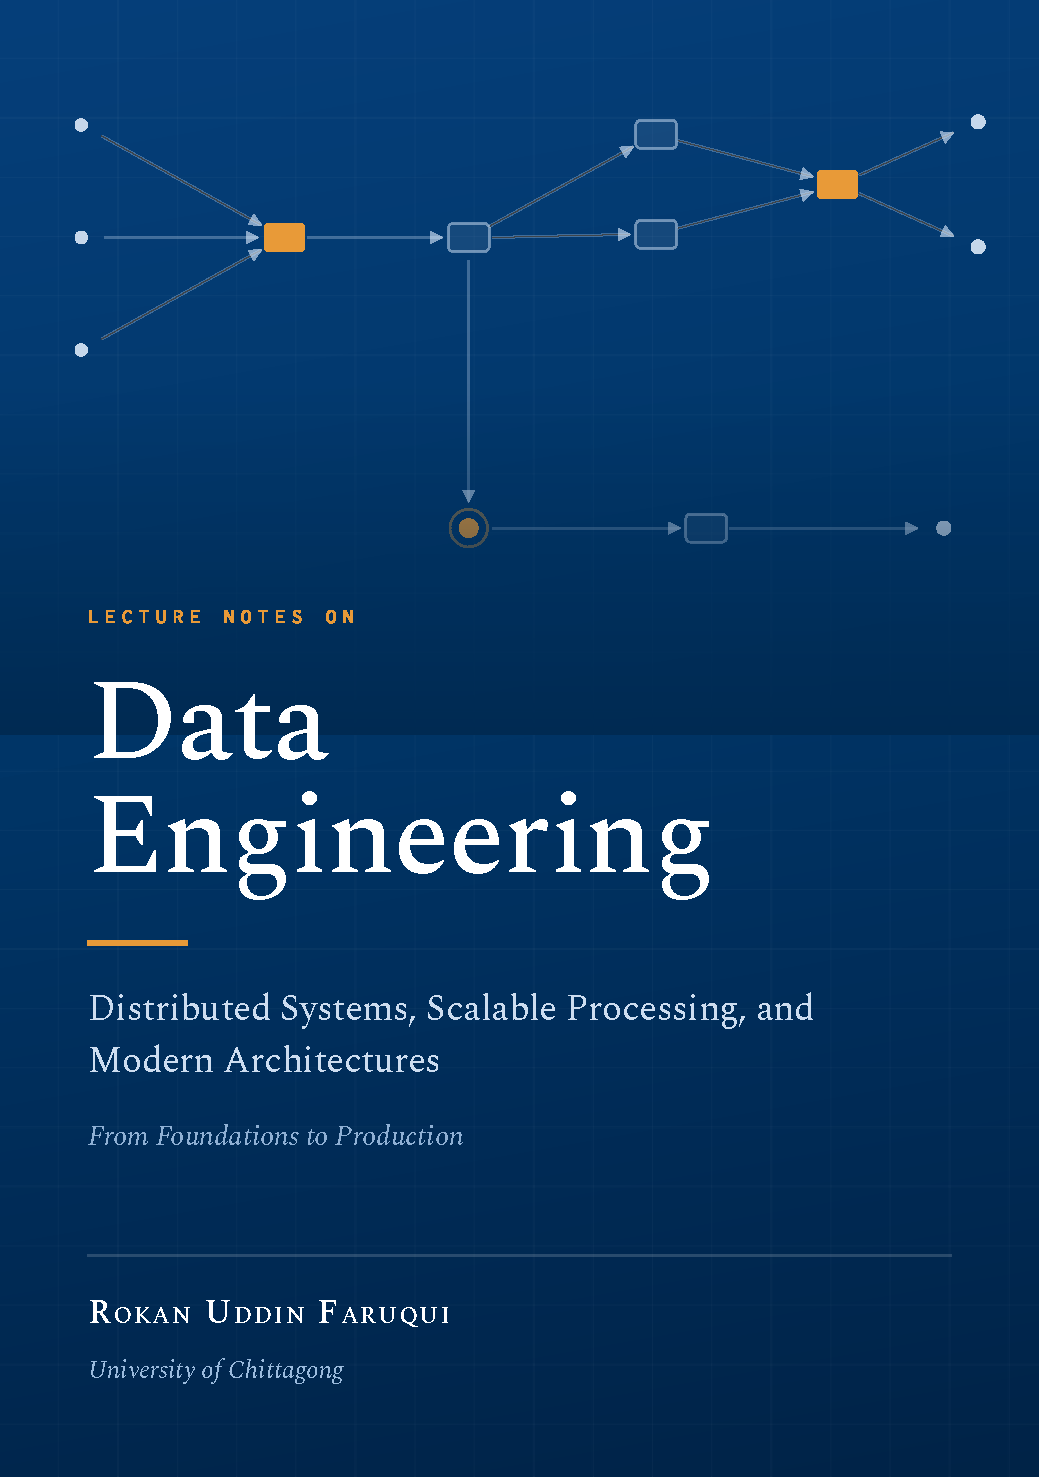
\includepdf[pages=1]{cover_v7.pdf}
%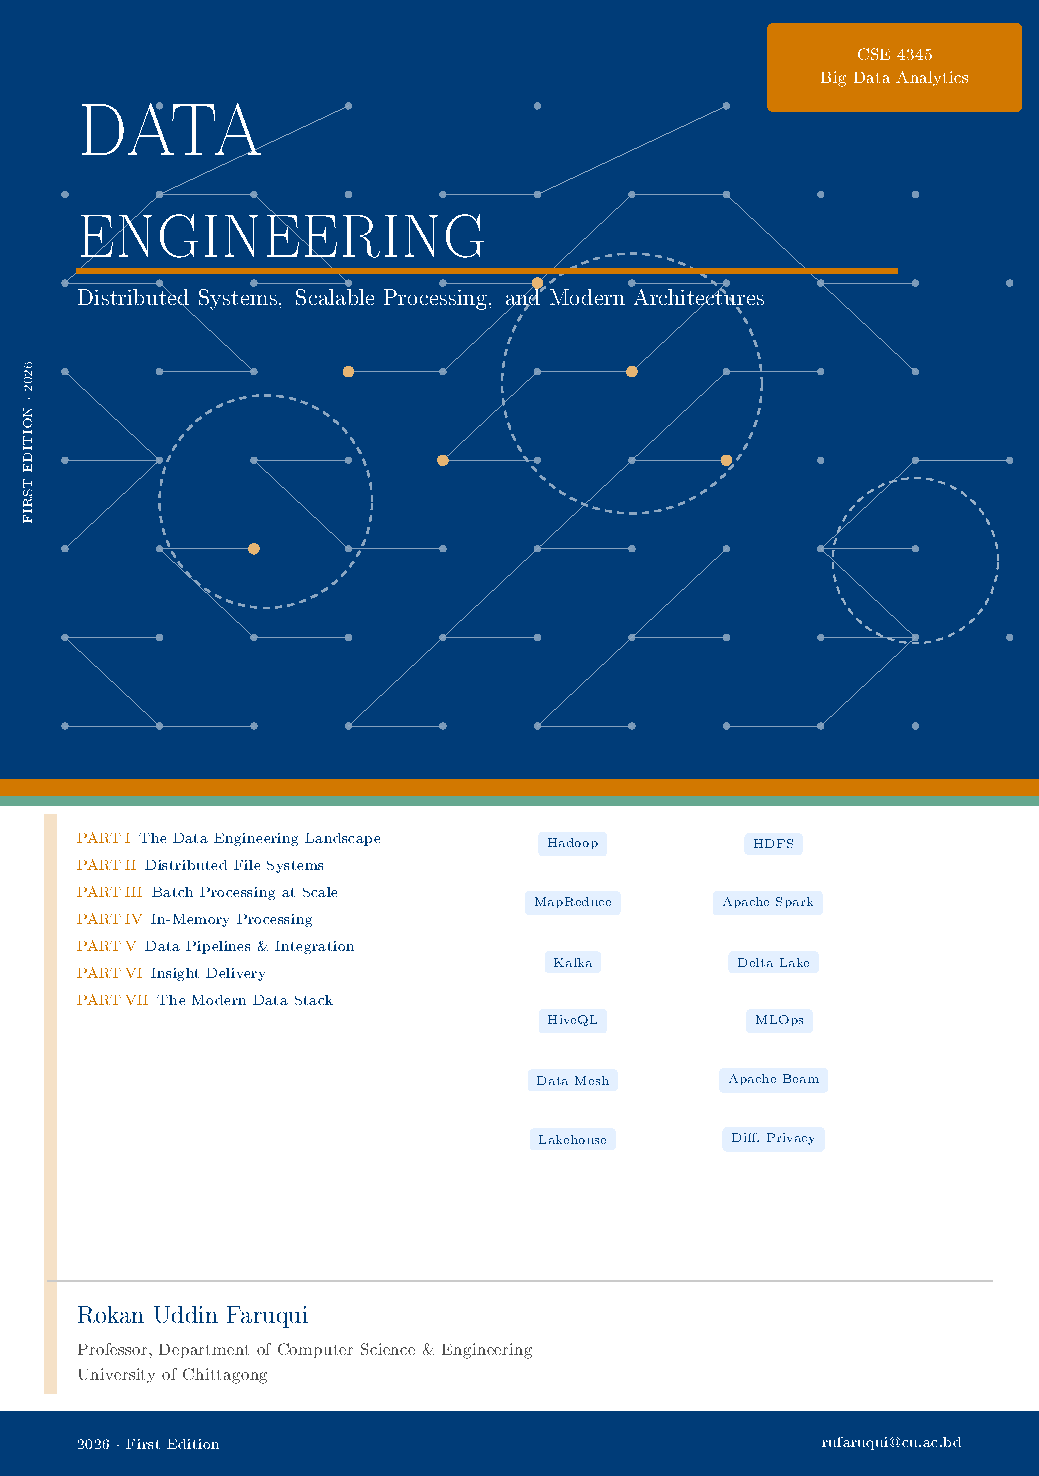
\includepdf[pages=1, fitpaper=true]{cover.pdf}

% Title + copyright page (single page between cover and ToC)
\cleardoublepage
\thispagestyle{empty}
\begin{center}
  \vspace*{2.2cm}

  {\color{DEBlue}\rule{\textwidth}{1.5pt}}
  \vspace{0.5cm}

  {\sffamily\Huge\bfseries\color{DEBlue} Data Engineering}

  \vspace{0.35cm}

  {\sffamily\Large\color{DEBlue!75}
    Distributed Systems, Scalable Processing,\\[4pt]
    and Modern Architectures}

  \vspace{0.35cm}
  {\color{DEBlue}\rule{\textwidth}{1.5pt}}

  \vspace{1.4cm}

  {\sffamily\large\bfseries \sc Rokan Uddin Faruqui}\\[5pt]
  {\sffamily\small Professor, Department of Computer Science \& Engineering}\\[2pt]
  {\sffamily\small University of Chittagong}

  \vspace{1.2cm}

  {\sffamily\small\color{DEGray}
    Lecture notes for \textbf{Big Data Analytics/Data Engineering} courses.\\[3pt] 
    Suitable for senior undergraduate and postgraduate study.}

  \vfill

  \noindent{\color{DEBlue!30}\rule{\textwidth}{0.6pt}}
  \vspace{0.35cm}

  {\sffamily\small\color{DEGray}
    \textit{First Edition, 2026.}\quad
    Licensed under \textbf{CC~BY~4.0} ---
    free to use, adapt, and distribute with attribution.\\[3pt]
    \texttt{creativecommons.org/licenses/by/4.0}}

  \vspace{0.4cm}
\end{center}

% Table of contents
\tableofcontents
% \listoffigures
% \listoftables

%----------------------------------------------------------------------
% MAIN CHAPTERS
%----------------------------------------------------------------------
\mainmatter

%%% Part I: The Data Engineering Landscape
\part{The Data Engineering Landscape}
%% ch01.tex — Chapter 1: The Big Data Revolution: Scale, Velocity, and Variety
%% Part of "Data Engineering" textbook

\chapter{The Big Data Revolution: Scale, Velocity, and Variety}
\label{ch:foundations}

\epigraph{\textit{``The world's most valuable resource is no longer oil, but data.''}}{The Economist, 2017}

\vspace{4pt}

\begin{chapterlearning}
After completing this chapter, you will be able to:
\begin{enumerate}
  \item Explain why traditional relational database systems cannot handle
        modern data workloads at scale, and identify the specific limits
        that are exceeded.
  \item Define the three original dimensions of big data (Volume,
        Velocity, Variety) and the two additional dimensions (Veracity,
        Value) that form the extended 5Vs framework.
  \item Classify any given data source as structured, semi-structured,
        or unstructured, and identify the appropriate storage and query
        tool for each category.
  \item Distinguish between vertical and horizontal scaling strategies,
        and explain why distributed, horizontally scaled systems dominate
        big data engineering.
  \item State the CAP theorem, explain the meaning of each property, and
        identify how real-world systems (HBase, Cassandra, PostgreSQL)
        position themselves in the CAP triangle.
  \item Compare batch and stream processing models and select the
        appropriate model for a given engineering requirement.
\end{enumerate}
\end{chapterlearning}

\bigskip

Every 60 seconds in 2024, users upload 500 hours of video to YouTube,
execute more than 5 million Google searches, send over one million
WhatsApp messages, and publish approximately 6,000 posts on X (formerly
Twitter). These figures are not curiosities; they represent a
fundamental transformation in the scale, speed, and diversity of data
that computing infrastructure is expected to handle. This chapter
establishes the conceptual and technical foundation for the entire
book. We begin by examining what makes data ``big,'' explore how that
bigness is formally characterized, and introduce the core theoretical
constraints---the CAP theorem in particular---that shape every
architectural decision in data engineering.

%%====================================================================
\section{Why Data Engineering Matters}
\label{sec:why-de}
%%====================================================================

In 2018, the International Data Corporation (IDC) projected that the
global \term{datasphere}---the total volume of data generated, captured,
copied, and consumed worldwide---would reach \textbf{175 zettabytes} by
2025, representing a 23-fold increase over the 7.2 ZB that existed in
2018 \parencite{IDC2018}. To appreciate this scale, consider that one
zettabyte equals $10^{21}$ bytes, or roughly 250 billion standard 4\TB\
hard drives---more drives than there are stars visible to the naked eye
from any single point on Earth.

\begin{table}[ht]
\centering
\caption{Data volume units and their relationship to everyday storage}
\label{tab:volume-units}
\renewcommand{\arraystretch}{1.3}
\begin{tabular}{L{2.4cm} R{2.4cm} L{6.0cm}}
\toprule
\textbf{Unit} & \textbf{Bytes} & \textbf{Illustrative equivalent} \\
\midrule
Kilobyte (KB)   & $10^{3}$  & A short email (plain text) \\
Megabyte (MB)   & $10^{6}$  & A 3-minute MP3 audio track \\
Gigabyte (GB)   & $10^{9}$  & A feature-length HD film \\
Terabyte (TB)   & $10^{12}$ & \textasciitilde310,000 photos from a 12 MP camera \\
Petabyte (PB)   & $10^{15}$ & All US academic research libraries combined \\
Exabyte (EB)    & $10^{18}$ & All words ever spoken by humans (estimated) \\
\textbf{Zettabyte (ZB)}  & $\mathbf{10^{21}}$ & \textbf{2025 global datasphere} \\
Yottabyte (YB)  & $10^{24}$ & Theoretical future scale \\
\bottomrule
\end{tabular}
\end{table}

Traditional \term{relational database management systems} (RDBMS)---the
dominant paradigm since Edgar Codd's foundational work in 1970---are
extraordinary tools for managing well-structured, bounded datasets. A
modern relational database running on a well-provisioned server can
comfortably manage tens of terabytes and sustain thousands of
transactions per second with full ACID guarantees. For a bank's
transaction ledger, a hospital's patient registry, or an airline's
reservation system, a carefully tuned relational system remains the
correct choice. The problem emerges when data characteristics exceed
what any single machine can handle: when datasets are measured in
petabytes rather than terabytes; when data arrives not from a single
transactional application but from millions of concurrent event streams;
and when the data itself is not neatly organized into rows and columns
but exists as images, audio recordings, sensor telemetry, and free-form
text. In these conditions, the fundamental assumptions of relational
database design break down.

\term{Data engineering} is the discipline concerned with the design,
construction, and maintenance of systems that collect, store, transform,
and serve large-scale data for downstream consumers---analysts, machine
learning models, business intelligence dashboards, and operational
applications. A data engineer builds the infrastructure that makes raw
data useful. This field draws on distributed systems, software
engineering, database theory, and applied computer science. The tools of
modern data engineering---distributed file systems, parallel batch
processors, in-memory computation engines, stream processing frameworks,
and pipeline orchestrators---are the subjects of this book.

\begin{keyinsight}{The Data Engineering Mandate}
Data engineering is not about \emph{generating} insight---that is the
domain of data science and analytics. Data engineering is about making
data \emph{available, reliable, and efficiently accessible} at any
scale. The data engineer builds the plumbing; analysts and scientists
use the water.
\end{keyinsight}

%%====================================================================
\section{Defining Big Data: The 3Vs Framework}
\label{sec:three-vs}
%%====================================================================

The term ``big data'' gained formal structure in 2001 when Doug Laney,
then a research analyst at the META Group, published a brief but
enormously influential research note identifying three dimensions along
which data management challenges had outpaced conventional tools
\parencite{Laney2001}. He labeled these dimensions \emph{Volume},
\emph{Velocity}, and \emph{Variety}---the \term{3Vs of big data}. Eleven
years later, Gartner (which had acquired META Group) codified these
dimensions into a formal definition:

\begin{defbox}{Big Data (Gartner/Beyer \& Laney, 2012)}
\textit{``Big data is high-volume, high-velocity and/or high-variety
information assets that demand cost-effective, innovative forms of
information processing that enable enhanced insight, decision making,
and process automation.''}\\[4pt]
\hfill --- Beyer \& Laney, Gartner Research, 2012 \parencite{GartnerBigData2012}
\end{defbox}

Each of the three dimensions corresponds to a distinct class of
engineering challenge. The McKinsey Global Institute, in its landmark
2011 study, reinforced this framing: big data refers to datasets
``whose size is beyond the ability of typical database software tools to
capture, store, manage and analyze'' \parencite{McKinsey2011}. Let us
examine each dimension in turn.

%--------------------------------------------------------------------
\subsection{Volume: The Scale Dimension}
\label{subsec:volume}
%--------------------------------------------------------------------

\term{Volume} refers to the sheer quantity of data that is generated,
accumulated, and must be stored and processed. Volume is the most
intuitively obvious characteristic of big data: a dataset is voluminous
when it exceeds the capacity of conventional tools---typically, when a
single machine cannot store and process it within an acceptable elapsed
time. The following production examples illustrate current operational
scales:

\begin{table}[ht]
\centering
\caption{Volume at production scale (representative 2023--2024 estimates)}
\label{tab:volume-examples}
\renewcommand{\arraystretch}{1.35}
\begin{tabular}{L{3.2cm} L{7.4cm}}
\toprule
\textbf{Organisation} & \textbf{Volume characteristic} \\
\midrule
Meta (Facebook)   & 500\TB\ of new data ingested per day across all platforms \\
Google            & $>$100\PB\ of data processed internally per day (estimated) \\
Walmart           & $>$2.5\PB\ of customer transaction data in analytical systems \\
CERN (LHC)        & $\approx$15\PB\ of particle collision data generated per year \\
Netflix           & $>$1\PB\ of user interaction events per day \\
NYSE              & $\approx$1\TB\ of trading records generated on a peak day \\
\bottomrule
\end{tabular}
\end{table}

From an engineering perspective, volume creates several concrete
challenges. First, no single server---even the highest-specification
available in 2024, with up to 64\TB\ of RAM---can hold a petabyte-scale
dataset in memory. Second, sequential reads from a single high-speed
SSD array proceed at approximately 7\GB/s; reading one petabyte at that
speed requires roughly 41 hours. Third, ingesting 500\TB\ per day means
sustained write throughput of approximately 5.8\GB/s, which no single
storage device can sustain reliably. The engineering response is
\emph{horizontal distribution}: partition data into blocks and spread
those blocks across a cluster of hundreds or thousands of commodity
machines---the approach formalized by the Google File System
\parencite{GFS2003} and, in open-source form, by Hadoop's HDFS
(discussed in Chapter~\ref{ch:hdfs}).

%--------------------------------------------------------------------
\subsection{Velocity: The Speed Dimension}
\label{subsec:velocity}
%--------------------------------------------------------------------

\term{Velocity} refers to the speed at which data is generated, arrives
at a system, and must be processed or acted upon. High-velocity data is
not merely large; it arrives \emph{continuously} and often demands
responses on timescales far shorter than batch processing can provide.

Consider a few representative velocities:
\begin{itemize}
  \item The Visa payment network processes approximately 24,000
        transactions per second at peak load.
  \item Global IoT deployments generate over one billion device sensor
        readings per hour across industrial, environmental, and consumer
        applications.
  \item A ride-sharing platform (such as Uber or Lyft) receives a GPS
        ping every three seconds from millions of simultaneously active
        drivers---at 5 million drivers, that is over 1.6 million
        location records per second.
  \item Modern stock exchanges publish quote updates for listed
        securities at rates exceeding one million messages per second
        during high-activity sessions.
\end{itemize}

The engineering challenge of velocity is distinct from that of volume:
a system may need to respond to each event within milliseconds (fraud
detection, payment authorization) or may tolerate latencies of seconds
(real-time dashboards). The key constraint is that high-velocity data
\emph{cannot wait} for a nightly batch process---by the time the batch
runs, the window for action has closed. This distinction drives the
separation between \emph{batch} and \emph{stream} processing
architectures, explored in Section~\ref{sec:batch-stream} and in depth
in Chapter~\ref{ch:pipelines}.

\begin{table}[ht]
\centering
\caption{The data processing spectrum by velocity requirement}
\label{tab:velocity-spectrum}
\renewcommand{\arraystretch}{1.35}
\begin{tabular}{L{2.2cm} L{1.6cm} L{3.2cm} L{3.4cm}}
\toprule
\textbf{Processing mode} & \textbf{Latency} & \textbf{Representative tools} & \textbf{Typical use case} \\
\midrule
Batch          & Hours      & Hadoop MapReduce, Hive & Nightly ETL, monthly billing \\
Micro-batch    & Seconds    & Spark Streaming        & Near-real-time dashboards \\
Stream         & Milliseconds & Apache Flink, Kafka Streams & Fraud detection, alerts \\
Real-time      & Sub-ms     & In-memory + Kafka      & Payment authorization \\
\bottomrule
\end{tabular}
\end{table}

%--------------------------------------------------------------------
\subsection{Variety: The Diversity Dimension}
\label{subsec:variety}
%--------------------------------------------------------------------

\term{Variety} refers to the diversity of data formats, types, schemas,
and sources that must be jointly ingested, stored, and analysed. Modern
organisations do not operate a single data source with a uniform schema;
they accumulate data from dozens of systems, each with its own format
and semantics.

Variety manifests along several axes. \emph{Format variety} arises when
data arrives as CSV files, JSON documents, XML feeds, binary Avro
records, columnar Parquet files, DICOM medical images, and MP4 video
simultaneously---all of which must be stored and queried together.
\emph{Source variety} arises when the same analytical question requires
joining data from relational databases, REST APIs, IoT sensor streams,
social media firehoses, and internal event logs. \emph{Semantic variety}
arises when a field named \texttt{date} means the transaction date in
one system, the record-entry date in another, and the customer birth
date in a third.

The foundational distinction among data types---structured,
semi-structured, and unstructured---is the key conceptual framework for
managing variety, and we explore it in detail in
Section~\ref{sec:data-taxonomy}.

\begin{researchspotlight}{Laney (2001) --- The Origin of the 3Vs}
\textbf{Citation:} Laney, D. (2001). \textit{3D Data Management:
Controlling Data Volume, Velocity and Variety}. META Group Research
Note 949, February 2001. \parencite{Laney2001}

\smallskip\noindent
\textbf{Key insight:} Laney's one-page note, written in the context of
e-commerce data challenges, framed data management as a three-dimensional
problem---not merely a storage problem. He argued that organisations
failing to address all three dimensions would face ``increasing
management headaches.''

\smallskip\noindent
\textbf{Technical contributions:}
\begin{itemize}
  \item Established the first formal vocabulary (\emph{3Vs}) for
        characterising modern data management challenges, unifying what
        had previously been treated as unrelated operational problems.
  \item Distinguished \emph{velocity} as a management dimension
        independent of volume---recognising that \emph{how fast} data
        arrives is as important as \emph{how much} arrives.
  \item Introduced \emph{variety} as the hardest dimension to manage,
        predicting the rise of semi-structured and unstructured data as
        dominant forms.
\end{itemize}

\smallskip\noindent
\textbf{Impact today:} The 3Vs framework is taught at every major
computer science programme and has been cited in thousands of academic
papers and industry reports. It remains the canonical definition of big
data, even as the framework has been extended to 5Vs and beyond. Gartner
officially adopted and extended the definition in 2012.
\end{researchspotlight}

%%====================================================================
\section{The Extended 5Vs Framework}
\label{sec:five-vs}
%%====================================================================

The 3Vs framework is powerful but incomplete. Two additional dimensions
have gained wide acceptance, bringing the framework to five:

\term{Veracity} refers to the trustworthiness and quality of data.
High-veracity data is accurate, consistent, and free of critical errors;
low-veracity data is noisy, inconsistent, or of uncertain provenance.
Veracity challenges arise in practical systems for many reasons: GPS
sensors drift by tens of metres in dense urban environments; optical
character recognition (OCR) on historical documents introduces
transcription errors; social media platforms contain significant volumes
of bot-generated content; and sensor networks may experience intermittent
failures that produce spurious or missing readings. The consequences of
low veracity can be severe---a machine learning model trained on
inaccurate data will make inaccurate predictions, regardless of how
sophisticated the model or how large the training set.

\term{Value} refers to the business or societal utility that can be
extracted from data. It is the ultimate justification for the
considerable engineering investment required to build big data systems.
A dataset may score highly on all four other Vs---petabytes of
high-velocity, highly varied, high-quality data---and still produce
no actionable insight if the right analytical questions are never asked,
or if the results are never operationalised. Value is the bridge between
technical capability and organisational outcomes.

\begin{table}[ht]
\centering
\caption{The 5Vs framework with engineering implications}
\label{tab:five-vs}
\renewcommand{\arraystretch}{1.45}
\begin{tabular}{L{1.8cm} L{3.2cm} L{3.5cm} L{2.6cm}}
\toprule
\textbf{Dimension} & \textbf{Definition} & \textbf{Production example} &
\textbf{Primary engineering challenge} \\
\midrule
Volume    & Scale of data generated and stored & Meta: 500\TB/day ingested &
            Distributed storage (HDFS, S3) \\
Velocity  & Speed of generation and processing & Visa: 24,000 tx/s &
            Stream processing (Kafka, Flink) \\
Variety   & Diversity of formats and sources & CSV + JSON + DICOM + MP4 &
            Schema integration, ETL/ELT \\
Veracity  & Trustworthiness of data quality & GPS drift, OCR errors, bot tweets &
            Data quality pipelines, validation \\
Value     & Business utility extracted from data & Fraud prevented, revenue gained &
            Feature engineering, ML pipelines \\
\bottomrule
\end{tabular}
\end{table}

\begin{researchspotlight}{McKinsey Global Institute (2011) --- Quantifying the Value Dimension}
\textbf{Citation:} Manyika, J.\ et~al.\ (2011). \textit{Big Data: The
Next Frontier for Innovation, Competition, and Productivity}. McKinsey
Global Institute, May 2011. \parencite{McKinsey2011}

\smallskip\noindent
\textbf{Key insight:} The report argued that big data has become ``a new
factor of production,'' alongside capital and labour---that is,
organisations with superior data capabilities will, over time,
systematically outperform those without them, in the same way that
access to capital separates competitive enterprises from struggling ones.

\smallskip\noindent
\textbf{Technical and economic contributions:}
\begin{itemize}
  \item Quantified the value potential across five major sectors:
        healthcare (\$300B+ annually in the US), public sector
        (\$250B+ in Europe), retail ($>$60\% operating margin
        improvement for early adopters), manufacturing, and personal
        location data.
  \item Identified the acute shortage of data-skilled talent as the
        primary constraint on value realisation---the report projected
        a shortfall of 140,000--190,000 professionals with deep
        analytical expertise in the US alone by 2018.
  \item Introduced the concept of ``data as infrastructure,'' arguing
        that the economic benefits of big data investment are broadly
        distributed across the economy, much like roads or electricity
        grids.
\end{itemize}

\smallskip\noindent
\textbf{Impact today:} This report is one of the most cited documents
in the history of data-driven business strategy. It directly influenced
technology investment priorities at major corporations and governments
worldwide, and it validated the creation of dedicated data engineering
and data science functions within large organisations.
\end{researchspotlight}

%%====================================================================
\section{A Taxonomy of Digital Data}
\label{sec:data-taxonomy}
%%====================================================================

Managing the Variety dimension of big data requires a clear
classification of data types. The field has converged on three primary
categories---structured, semi-structured, and unstructured---distinguished
principally by the presence, flexibility, and location of their schema.

%--------------------------------------------------------------------
\subsection{Structured Data}
\label{subsec:structured}
%--------------------------------------------------------------------

\begin{defbox}{Structured Data}
Data organised according to a \textbf{predefined, rigid schema} in which
every record contains the same fields in the same order, with each field
having a specified data type. The schema is defined and enforced before
data is written (\textbf{schema-on-write}). Structured data is typically
stored in relational database management systems and queryable directly
with standard SQL.
\end{defbox}

Structured data represents the most mature and well-understood category.
Relational database theory, developed by Codd (1970) and refined over
five decades, provides powerful tools for storing, querying, and
maintaining the integrity of structured data. A bank's transaction ledger
is a canonical example: every row has an account number, a timestamp, an
amount, a currency code, and a transaction type. There are no optional
fields, no embedded documents, no ambiguous formats. SQL can answer
virtually any analytical question over such data with high efficiency.

The primary limitation of structured data is its rigidity. Adding a new
column to a table with hundreds of millions of rows requires a schema
migration---a costly, time-consuming, and potentially disruptive
operation. More fundamentally, many of the most valuable data types in
modern organisations---customer reviews, support transcripts, medical
images, sensor streams---cannot be naturally represented in rows and
columns without destructive simplification. Despite this, structured data
remains the bedrock of transactional systems, and big data engineering
tools like \tool{Apache Sqoop} exist specifically to migrate structured
data from RDBMS sources into distributed analytical systems (covered in
Chapter~\ref{ch:pipelines}).

In terms of global prevalence, structured data accounts for only
approximately 20\% of all digital data---yet it represents the most
well-governed, analysable slice of that data.

%--------------------------------------------------------------------
\subsection{Semi-Structured Data}
\label{subsec:semi-structured}
%--------------------------------------------------------------------

\begin{defbox}{Semi-Structured Data}
Data with a \textbf{flexible, self-describing schema} embedded within
the data itself. Fields are identified by keys or tags that travel with
the record, not by position in a fixed row. New fields can be added
without modifying a central schema registry. Semi-structured data is
typically stored as files or in NoSQL databases and processed with a
\textbf{schema-on-read} approach: the schema is imposed at query time,
not at write time.
\end{defbox}

Semi-structured data dominates modern web and application architectures.
The two most prevalent formats are \textbf{JSON} (JavaScript Object
Notation) and \textbf{XML} (Extensible Markup Language):

\begin{lstlisting}[style=pseudocode, caption={A JSON event record from a streaming API}]
{
  "event_id":   "e-928471",
  "event_type": "page_view",
  "timestamp":  "2024-03-15T14:22:31Z",
  "user": {
    "id":       "u-441982",
    "tier":     "premium"
  },
  "page":       "/product/laptop-x500",
  "session_ms": 4820,
  "metadata": {
    "user_agent": "Mozilla/5.0 ...",
    "referrer":   "https://search.example.com"
  }
}
\end{lstlisting}

Notice that the JSON record carries its own field names (``event\_id'',
``timestamp'', ``user'', etc.) directly within the data. A consumer
reading this record does not need to consult an external schema
definition to know what each field means. This \emph{self-description}
property makes semi-structured data highly flexible: a downstream
service that only cares about \texttt{event\_type} and
\texttt{user.tier} can simply ignore all other fields. When a new field
(e.g., \texttt{ab\_test\_variant}) must be added, it can be appended to
future records without invalidating existing ones.

The schema-on-read approach enabled by semi-structured formats is
central to the \emph{data lake} architecture: data is ingested in its
native format without transformation, and the schema is applied by the
analytical tool at query time. This defers the cost of schema design
but introduces the risk of schema drift---where the meaning or format
of a field changes silently between producers, creating silent data
quality failures. Managing this risk (through schema registries,
contract testing, and data lineage tracking) is a significant part of
production data engineering practice.

Web server access logs, IoT device telemetry published via MQTT,
REST API responses, email headers, configuration files in YAML or TOML,
and Apache Avro records with embedded schemas all belong to the
semi-structured category. This category accounts for roughly 10\% of
global data by volume.

%--------------------------------------------------------------------
\subsection{Unstructured Data}
\label{subsec:unstructured}
%--------------------------------------------------------------------

\begin{defbox}{Unstructured Data}
Data with \textbf{no predefined schema} and no embedded key-value
structure that can be directly queried. The semantic content is encoded
in the raw signal---pixels, audio samples, token sequences---and cannot
be accessed by a relational or document query engine without substantial
preprocessing (feature extraction, natural language processing, or
computer vision).
\end{defbox}

Unstructured data is the dominant form of digital data, accounting for
an estimated 70--80\% of the global datasphere. It encompasses text
documents (news articles, legal contracts, clinical notes, social media
posts), images (medical scans, satellite photography, product
photographs), audio recordings (call-centre conversations, podcasts,
speech-enabled device logs), video (surveillance footage, user-generated
content, manufacturing inspection recordings), and raw sensor streams
(seismic signals, EEG waveforms, raw GPS trajectories).

The defining challenge of unstructured data is that extracting
information requires \emph{interpretation}---a step that structured and
semi-structured data largely skip. A relational database can compute the
average transaction amount in a single SQL aggregation; answering the
question ``what is the sentiment of customer reviews mentioning our new
product?'' requires tokenising text, building or loading a language
model, running inference, and aggregating the model's output. This
computational chain is far more complex and resource-intensive, which is
why the tools introduced in later chapters---Spark MLlib, distributed
deep learning frameworks, and specialised feature stores---are essential
components of modern data engineering systems.

\begin{table}[ht]
\centering
\caption{Comparison of data type characteristics and engineering implications}
\label{tab:data-type-comparison}
\renewcommand{\arraystretch}{1.45}
\begin{tabular}{L{2.0cm} L{2.6cm} L{2.6cm} L{2.8cm}}
\toprule
\textbf{Dimension}       & \textbf{Structured}     & \textbf{Semi-structured}  & \textbf{Unstructured} \\
\midrule
Schema                   & Predefined, rigid        & Self-describing, flexible & Absent \\
Schema timing            & On write                 & On read                   & N/A \\
Storage                  & RDBMS tables             & Files, NoSQL, APIs        & Object stores, HDFS \\
Query tool               & SQL                      & JSONPath, Hive, Spark SQL & NLP, CV, Spark MLlib \\
Global share             & $\sim$20\%               & $\sim$10\%                & $\sim$70--80\% \\
Schema change cost       & High (migration)         & Low                       & N/A \\
Typical ingestion tool   & Sqoop                    & Kafka, Flume              & Custom pipelines \\
\textbf{Examples}        & Bank ledger, ERP records & REST API JSON, server logs & MRI scan, audio call \\
\bottomrule
\end{tabular}
\end{table}

\begin{caution}{JSON is Semi-Structured, Not Unstructured}
A frequent and consequential error: classifying JSON or XML as
``unstructured'' because it does not look like a database table. JSON
and XML carry an embedded schema in the form of key names and
hierarchical nesting. A query engine can navigate this structure
directly (using JSONPath, XPath, or Hive's schema-on-read). An MRI
scan, a JPEG image, or an MP3 recording carries \emph{no} such
navigable schema---its semantic content is encoded in the binary signal
itself, requiring a domain-specific model (computer vision, speech
recognition) to interpret. The distinction matters architecturally:
semi-structured data can be stored and queried in a data lake with
minimal transformation; unstructured data requires a preprocessing
pipeline before it becomes analytically useful.
\end{caution}

%%====================================================================
\section{The Engineering Response to Scale}
\label{sec:engineering-response}
%%====================================================================

Given the 3Vs, the engineering question is: how do we build systems
capable of storing petabytes, processing millions of events per second,
and integrating dozens of heterogeneous data sources? The answer, which
runs through every chapter of this book, reduces to a small set of
foundational principles.

%--------------------------------------------------------------------
\subsection{Vertical vs.\ Horizontal Scaling}
\label{subsec:scaling}
%--------------------------------------------------------------------

There are two ways to make a computing system more powerful.
\term{Vertical scaling} (scaling up) means adding more resources to a
single machine: a faster processor, more RAM, a larger or faster storage
array. Vertical scaling is simple---it introduces no distributed-systems
complexity---but it has a hard physical ceiling. The most powerful
single-node servers available in 2024 top out at approximately 64\TB\
of RAM and a handful of high-throughput storage controllers. Above this
limit, no amount of money can buy a single machine large enough to hold
the dataset. Vertical scaling is also exponentially expensive: a server
with twice the RAM costs approximately eight times as much.

\term{Horizontal scaling} (scaling out) means adding more machines to a
cluster and distributing the data and computation across all of them.
Each individual machine is a commodity server costing between three and
eight thousand dollars. The power of the cluster grows nearly linearly
with the number of nodes added: doubling the number of nodes
approximately doubles the throughput. Failure of a single node---which
is expected, not exceptional, in a large cluster---does not halt the
system, because data is replicated across multiple nodes.

\begin{table}[ht]
\centering
\caption{Vertical vs.\ horizontal scaling: a systematic comparison}
\label{tab:scaling}
\renewcommand{\arraystretch}{1.4}
\begin{tabular}{L{2.8cm} L{3.3cm} L{3.9cm}}
\toprule
\textbf{Attribute}        & \textbf{Vertical (Scale Up)}  & \textbf{Horizontal (Scale Out)} \\
\midrule
Scalability ceiling       & Hard physical limit ($\sim$64\TB\ RAM) & Near-unlimited (add nodes) \\
Cost scaling              & Superlinear (exponential)    & Near-linear per node \\
Fault model               & Single point of failure      & Tolerates individual node failures \\
Complexity                & Low (no distributed systems) & High (consistency, coordination) \\
Latency for small queries & Low                          & Higher (network overhead) \\
Typical cost example      & Oracle Exadata: $>$\$500K/yr & 1,000 nodes $\times$ \$5K = \$5M (one-time) \\
\textbf{Used by}          & Traditional RDBMS, data warehouses & Hadoop, Spark, Cassandra, Kafka \\
\bottomrule
\end{tabular}
\end{table}

%--------------------------------------------------------------------
\subsection{The Commodity Hardware Insight}
\label{subsec:commodity}
%--------------------------------------------------------------------

The observation that underpins all of distributed data engineering is
deceptively simple: \emph{commodity hardware will fail, and systems must
be designed with this expectation from the start}. In a cluster of 1,000
commodity servers, with each server having a disk failure rate of 1\% per
year, we expect approximately 10 disk failures per year---about one every
five weeks. At 10,000 nodes (the scale of Yahoo!'s first production
Hadoop cluster in 2008), this becomes roughly one disk failure per day.
The solution is not to prevent failures---that is neither economically
nor physically feasible---but to design for them. Every piece of data is
stored in multiple copies on different nodes; if one node fails, the data
remains available from the surviving copies, and the system automatically
creates a new replica on a healthy node. This design principle, first
articulated for distributed file systems by Google's engineers
\parencite{GFS2003}, is the cornerstone of HDFS, Kafka, and Cassandra
alike.

%--------------------------------------------------------------------
\subsection{Moving Computation to Data}
\label{subsec:comp-to-data}
%--------------------------------------------------------------------

The second foundational principle of distributed data processing inverts
the traditional computing model. In a conventional system, data is moved
to the processor: a query is issued, data is fetched from storage into
RAM, and the CPU processes it. This model fails at petabyte scale because
the network bandwidth required to move large amounts of data to a central
processor becomes the bottleneck---the network simply cannot move data
fast enough to keep the processor busy.

The solution, pioneered by Google's MapReduce system \parencite{MapReduce2004}
and implemented in every major big data processing framework, is to
\emph{move computation to the data}: send the processing logic (a
function or query) to the node where the relevant data blocks reside,
execute the computation locally, and collect only the (smaller) results.
This principle---\textbf{data locality}---drastically reduces network
traffic and enables the aggregate CPU capacity of an entire cluster to be
applied in parallel to a large dataset.

\begin{systemdesign}{Data Locality in Practice}
In HDFS (Chapter~\ref{ch:hdfs}), a 128\MB\ data block is stored on three
nodes. When a MapReduce or Spark job must process that block, the
scheduler first attempts to assign the task to one of the three nodes
already holding a replica (task-local scheduling). If those nodes are
busy, it next tries a node on the same physical rack (rack-local
scheduling). Only if no rack-local node is available does it resort to
sending the data over the network. In production clusters, over 90\% of
tasks execute with data locality, meaning almost all processing is local
I/O rather than network transfer.
\end{systemdesign}

%%====================================================================
\section{The CAP Theorem}
\label{sec:cap}
%%====================================================================

Building a distributed system---one that spans multiple machines
connected by a network---introduces a fundamental theoretical constraint
that shapes every storage and database design decision in data
engineering. This constraint is captured by the \term{CAP theorem}.

%--------------------------------------------------------------------
\subsection{Statement and Definitions}
\label{subsec:cap-statement}
%--------------------------------------------------------------------

The CAP theorem was conjectured by Eric Brewer in his keynote address at
the ACM Symposium on Principles of Distributed Computing in 2000
\parencite{Brewer2000} and formally proved by Gilbert and Lynch two years
later \parencite{GilbertLynch2002}. It states:

\begin{defbox}{The CAP Theorem (Brewer, 2000; Gilbert \& Lynch, 2002)}
A distributed data system can simultaneously guarantee \textbf{at most
two} of the following three properties:
\begin{enumerate}
  \item \textbf{Consistency (C):} Every read operation returns the most
        recent successfully written value, or an error. All nodes in the
        system see the same data at the same time.
  \item \textbf{Availability (A):} Every request to a non-failed node
        receives a response---not guaranteed to be the most recent
        write, but a response nonetheless.
  \item \textbf{Partition Tolerance (P):} The system continues to
        operate correctly even if an arbitrary number of messages
        between nodes are lost or delayed (a \emph{network partition}).
\end{enumerate}
\end{defbox}

Understanding what each property means in operational terms is essential
for reasoning about system design. \emph{Consistency}, in the CAP sense,
is not the same as the C in ACID transactions (which refers to
maintaining database invariants); CAP consistency is \emph{linearisability}---
the guarantee that every read sees the most recent write, as if all
operations occurred on a single machine. \emph{Availability} means every
request gets a response; it does not mean the response contains current
data. \emph{Partition tolerance} means the system continues to function
when the network splits into disconnected sub-clusters.

%--------------------------------------------------------------------
\subsection{The Practical Implication: Choosing C vs.\ A}
\label{subsec:cap-practice}
%--------------------------------------------------------------------

The critical practical insight is that network partitions in distributed
systems are not theoretical edge cases---they are \emph{inevitable}. Any
system operating across multiple machines connected by a real network
will, at some point, experience a partition: a switch failure, a
misconfigured firewall rule, a miscabling in a data centre, or a brief
network congestion event that causes messages to be delayed or dropped.
Therefore, in any real distributed system, partition tolerance (P) is
not optional. A system that cannot tolerate partitions is effectively a
single-machine system.

Given that P is always required, the CAP theorem reduces to a binary
choice: when a partition occurs, should the system prioritise
\textbf{consistency} (refuse requests that cannot be answered with
current data, guaranteeing accuracy) or \textbf{availability} (answer
every request with possibly stale data, guaranteeing responsiveness)?
This choice is one of the most important architectural decisions in data
engineering.

\begin{figure}[ht]
\centering
\begin{tikzpicture}[
    node distance=0pt,
    corner/.style={font=\small\bfseries\sffamily, text=DEBlue, align=center},
    edge lbl/.style={font=\scriptsize\sffamily, align=center},
    sys/.style={font=\scriptsize\ttfamily, align=center},
    blob/.style={draw=none, rounded corners=3pt, inner sep=3pt, align=center,
                 font=\scriptsize\sffamily}
  ]
  % Triangle vertices
  \coordinate (C) at (0, 5.2);
  \coordinate (A) at (-4.2, 0);
  \coordinate (P) at (4.2, 0);

  % Triangle
  \draw[DEBlue, very thick] (C) -- (A) -- (P) -- cycle;

  % Vertex labels
  \node[corner] at (0, 5.7)    {Consistency (C)};
  \node[corner] at (-4.9, -0.4) {Availability (A)};
  \node[corner] at (4.9, -0.4)  {Partition Tolerance (P)};

  % CA zone (top left edge)
  \node[blob, fill=DELightBlue] at (-2.8, 3.2) {%
    \textbf{CA} systems\\[2pt]
    PostgreSQL, MySQL\\
    (single-datacenter)
  };

  % CP zone (top right edge)
  \node[blob, fill=DELightGreen] at (2.8, 3.2) {%
    \textbf{CP} systems\\[2pt]
    Apache HBase\\
    ZooKeeper
  };

  % AP zone (bottom)
  \node[blob, fill=DELightAccent] at (0, 0.9) {%
    \textbf{AP} systems\\[2pt]
    Apache Cassandra\\
    Amazon DynamoDB
  };

  % Edge descriptors
  \node[edge lbl, rotate=52, text=DEBlue!60] at (-1.8, 2.4)
        {no partition\\tolerance};
  \node[edge lbl, rotate=-52, text=DEBlue!60] at (1.8, 2.4)
        {sacrifices\\availability};
  \node[edge lbl, text=DEBlue!60] at (0, -0.4)
        {sacrifices consistency};
\end{tikzpicture}
\caption{The CAP triangle: every distributed system chooses two of the three properties.
         Because network partitions are unavoidable, real systems choose between CP and AP.}
\label{fig:cap-triangle}
\end{figure}

\begin{table}[ht]
\centering
\caption{CAP positioning of representative data systems}
\label{tab:cap-systems}
\renewcommand{\arraystretch}{1.4}
\begin{tabular}{L{2.8cm} C{0.8cm} L{5.4cm}}
\toprule
\textbf{System} & \textbf{CAP} & \textbf{Design rationale} \\
\midrule
PostgreSQL, MySQL & CA & Designed for single-node or tightly coupled clusters;
                         cannot tolerate true network partitions \\
Apache HBase      & CP & Chooses consistency: if a partition occurs, HBase may
                         become unavailable rather than serve stale data \\
Apache ZooKeeper  & CP & Coordination service where serving stale configuration
                         data would be catastrophic \\
Apache Cassandra  & AP & Chooses availability: always responds, using
                         tunable eventual consistency (read your own writes) \\
Amazon DynamoDB   & AP & Optimised for always-on e-commerce workloads where
                         availability is paramount \\
\bottomrule
\end{tabular}
\end{table}

\begin{researchspotlight}{Brewer (2000) and Gilbert \& Lynch (2002) --- The CAP Theorem}
\textbf{Citations:}
\begin{itemize}
  \item Brewer, E.A.\ (2000). \textit{Towards Robust Distributed Systems}.
        Keynote, PODC 2000. \parencite{Brewer2000}
  \item Gilbert, S.\ \& Lynch, N.A.\ (2002). Brewer's Conjecture and the
        Feasibility of Consistent, Available, Partition-Tolerant Web
        Services. \textit{ACM SIGACT News}, 33(2):51--59.
        \parencite{GilbertLynch2002}
\end{itemize}

\smallskip\noindent
\textbf{Key insight:} Brewer's conjecture, presented as intuition in
2000, was that three desirable properties of distributed systems could
not all be simultaneously guaranteed. Gilbert and Lynch provided a
formal proof two years later, elevating the observation from engineering
folklore to a mathematically rigorous theorem.

\smallskip\noindent
\textbf{Technical contributions:}
\begin{itemize}
  \item Provided the formal definitions of consistency (linearisability),
        availability, and partition tolerance used in distributed systems
        theory.
  \item Proved that no distributed system can achieve all three
        properties simultaneously using an asynchronous network model.
  \item Established the vocabulary (CA, CP, AP) that data architects use
        to describe and compare distributed systems.
\end{itemize}

\smallskip\noindent
\textbf{Nuance and evolution:} The CAP theorem is often oversimplified.
Eric Brewer himself, in a 2012 retrospective, noted that the choice is
not always a binary C-vs-A decision: systems like DynamoDB offer tunable
consistency levels, allowing different operations to trade consistency
for availability at the operation level. The PACELC model (Patterson
et~al., 2012) extends CAP by noting that even without a partition,
systems must trade latency for consistency---a trade-off CAP does not
capture. Despite these refinements, the CAP theorem remains the most
widely cited result in distributed systems theory.
\end{researchspotlight}

%%====================================================================
\section{Batch vs.\ Stream Processing}
\label{sec:batch-stream}
%%====================================================================

The Velocity dimension of big data---the need to process data that
arrives continuously and at high rates---has driven the development of
two fundamentally different processing paradigms that data engineers must
understand and choose between.

%--------------------------------------------------------------------
\subsection{Batch Processing}
\label{subsec:batch}
%--------------------------------------------------------------------

\term{Batch processing} operates on a fixed, bounded dataset accumulated
over a period of time. The data is first stored in full (on disk, in a
distributed file system, or in a data warehouse), and then a
computation---the \emph{batch job}---is run over the entire stored
dataset. Classic examples include nightly financial reconciliation, end-of-month
billing, weekly machine learning model retraining, and annual census
analysis.

Batch processing has several important properties. First, it achieves
very high \emph{throughput}: because the entire dataset is available
before processing begins, the job can be optimised for sequential I/O,
sorted reads, and massive parallelism. Second, batch jobs are inherently
\emph{reproducible}: re-running the same job on the same input data will
always produce the same output---a property critical for auditing and
debugging. Third, batch jobs can be \emph{fault-tolerant} in a simple
way: if a task fails, it can be restarted from the last checkpoint
without affecting the rest of the job. Fourth, and most importantly for
our purposes, batch processing has \emph{latency measured in hours}: a
nightly ETL job that begins at 02:00 and finishes at 06:00 delivers
results four hours after the data cutoff. For applications that need to
respond to data within seconds or milliseconds, this latency is
unacceptable.

%--------------------------------------------------------------------
\subsection{Stream Processing}
\label{subsec:stream}
%--------------------------------------------------------------------

\term{Stream processing} operates on an unbounded, continuously arriving
sequence of data records. Rather than accumulating data and running a
batch job, a stream processing engine processes each record (or a
small micro-batch of records) as it arrives, maintaining running
state across the stream. The key characteristic is \emph{low latency}:
a stream processor can emit results within milliseconds to seconds of
each event's arrival.

Stream processing is the appropriate model for applications where the
value of a response decays rapidly with time: real-time fraud detection
(a stolen card must be blocked before the second transaction clears, not
after nightly batch analysis); live stock market monitoring (an
algorithmic trading system needs the current quote, not yesterday's
close); operational dashboards (a call-centre manager needs to see
current queue depth, not yesterday's average); and anomaly detection in
industrial systems (a turbine failure signal is valuable in real time,
not eight hours later).

Stream processing introduces engineering challenges that batch processing
avoids. Records may arrive \emph{out of order} (a mobile device's
network connection may be intermittent, causing events to be delayed and
arrive after later events). Events may carry an \emph{event time}
(when something happened) that differs from \emph{processing time}
(when the event arrived at the system). Stateful computations---for
example, counting the number of page views per user in the past
60 minutes---must be maintained across an infinite stream, requiring
careful memory management and state backends. Fault recovery requires
mechanisms like \emph{exactly-once processing} semantics, which add
significant implementation complexity.

\begin{table}[ht]
\centering
\caption{Batch vs.\ stream processing: a systematic comparison}
\label{tab:batch-stream}
\renewcommand{\arraystretch}{1.45}
\begin{tabular}{L{2.6cm} L{3.1cm} L{3.9cm}}
\toprule
\textbf{Attribute}      & \textbf{Batch processing}    & \textbf{Stream processing} \\
\midrule
Data model              & Bounded, stored dataset      & Unbounded, continuously arriving events \\
Latency                 & Minutes to hours             & Milliseconds to seconds \\
Throughput              & Very high                    & Moderate (per-event overhead) \\
Fault recovery          & Re-run from checkpoint       & Exactly-once semantics required \\
State management        & Simple (no persistent state) & Complex (stateful operators, windows) \\
Out-of-order data       & Not a concern                & Central challenge (watermarks) \\
Debugging               & Easy (fixed inputs/outputs)  & Hard (live, non-reproducible) \\
Typical tools           & Hadoop MapReduce, Hive, Spark Batch & Kafka, Apache Flink, Spark Streaming \\
\textbf{Use cases}      & ETL, ML training, billing    & Fraud detection, monitoring, alerts \\
\bottomrule
\end{tabular}
\end{table}

\begin{keyinsight}{Lambda and Kappa Architectures}
Many production systems need both low latency \emph{and} high
accuracy---properties that are difficult to achieve simultaneously. The
\textbf{Lambda architecture} (Nathan Marz, 2011) addresses this by
running both a batch layer (for accurate, comprehensive historical
analysis) and a speed layer (for low-latency approximate results) in
parallel, merging their outputs in a serving layer. The cost is
engineering complexity: every transformation must be implemented twice,
in different frameworks. The \textbf{Kappa architecture} (Jay Kreps,
2014) simplifies this by replacing the batch layer with a replay of the
full event log through the stream processor---using Apache Kafka's
message retention to make historical reprocessing possible through the
streaming path. Both architectures are examined in depth in
Chapter~\ref{ch:pipelines}.
\end{keyinsight}

%%====================================================================
\section{Case Study: Walmart's Retail Analytics Platform}
\label{sec:walmart-case}
%%====================================================================

\begin{casestudy}{Walmart --- Petabyte-Scale Retail Intelligence}

\textbf{Background.}
Walmart is the world's largest retailer by revenue, operating over
10,000 stores across 27 countries and serving approximately 230 million
customers per week. The scale of its data generation is correspondingly
vast: every store transaction, supply chain event, website interaction,
and third-party demand signal contributes to what is one of the largest
private-sector data repositories in existence.

\smallskip
\textbf{Scale.}
Walmart's internal data analytics environment holds over \textbf{2.5
petabytes} of customer transaction data in its core analytics systems,
with an additional multi-petabyte tier of raw, unstructured data in its
data lake. The company processes roughly one million customer
transactions \emph{per hour}---approximately 280 transactions per second
on a typical day, with significant spikes during seasonal events
(Thanksgiving weekend in the United States generates transaction volumes
three to four times the average daily rate).

\smallskip
\textbf{Data variety.}
Walmart's analytical systems must integrate across all three data
categories described in this chapter:
\begin{itemize}
  \item \textbf{Structured:} Point-of-sale transaction records
        (item, quantity, price, timestamp, store ID, payment method)
        from 10,000+ stores, all originally stored in Oracle RDBMS systems.
  \item \textbf{Semi-structured:} Web and mobile clickstream events in
        JSON format (product views, search queries, cart additions,
        checkout abandonment events) from Walmart.com.
  \item \textbf{Unstructured:} Customer product reviews, call-centre
        transcript audio, and supplier-submitted product imagery for
        catalogue enrichment.
\end{itemize}

\smallskip
\textbf{Engineering challenges and solutions.}
The 3Vs framework maps directly onto Walmart's operational realities:

\begin{itemize}
  \item \textbf{Volume:} Transaction data accumulated over decades cannot
        fit in any single RDBMS. Walmart migrated its analytical
        workloads to a Hadoop-based data lake, using HDFS for distributed
        storage and \tool{Apache Hive} for SQL-style querying over PB-scale
        datasets.
  \item \textbf{Velocity:} Supply chain decisions---whether to redistribute
        inventory across distribution centres---must respond to real-time
        demand signals, not yesterday's batch report. Walmart deployed
        Apache Kafka for real-time event streaming and uses stream
        processing for demand sensing.
  \item \textbf{Variety:} Integrating transaction records, clickstream
        events, weather data (a known driver of consumer behaviour), and
        social media sentiment requires a data integration pipeline that
        handles schema mismatches, different temporal granularities, and
        inconsistent entity representations (the same product may have
        different identifiers in the RDBMS and the web catalogue).
\end{itemize}

\smallskip
\textbf{Business outcomes.}
Walmart's investment in big data engineering has enabled demand
forecasting accuracy that reduced food waste by 15--20\% in its grocery
divisions (reducing spoilage by anticipating demand more precisely), and
dynamic pricing algorithms that run across its full product catalogue
multiple times per day. During the COVID-19 pandemic, real-time analytics
over social media and purchase patterns allowed Walmart to anticipate
demand surges for sanitisers, masks, and canned goods several days before
they peaked---enabling pre-positioning of inventory that proved critical
when supply chains became constrained.

\smallskip
\textbf{Lesson.}
Walmart's evolution from single-RDBMS analytics to a multi-petabyte
distributed data platform illustrates the core thesis of this book: the
3Vs are not abstract concepts but concrete engineering constraints that
force specific architectural choices. Every tool introduced in subsequent
chapters exists because organisations like Walmart encountered these
constraints and could not solve them with conventional technology.
\end{casestudy}

%%====================================================================
\section*{Chapter Summary}
\label{sec:ch1-summary}
%%====================================================================

This chapter established the conceptual and theoretical foundations for
the rest of the book. The key points are:

\begin{itemize}
  \item The global datasphere is projected to reach 175 ZB by 2025,
        driven by social media, IoT, commerce, and scientific
        instrumentation. Traditional RDBMS cannot manage data at this
        scale.

  \item \textbf{Data engineering} is the discipline of building
        infrastructure that makes large-scale data available, reliable,
        and efficiently queryable for downstream consumers.

  \item The \textbf{3Vs framework} (Laney, 2001) characterises big data
        along three dimensions: \emph{Volume} (scale), \emph{Velocity}
        (speed), and \emph{Variety} (diversity). The extended \textbf{5Vs}
        adds \emph{Veracity} (data quality) and \emph{Value} (business
        utility).

  \item Digital data falls into three categories: \textbf{structured}
        (predefined schema, schema-on-write, $\sim$20\% of global data),
        \textbf{semi-structured} (self-describing schema, schema-on-read,
        $\sim$10\%), and \textbf{unstructured} (no schema, requires
        ML/NLP/CV to interpret, $\sim$70--80\%).

  \item \textbf{Horizontal scaling} (adding commodity nodes) is the
        dominant strategy for big data infrastructure because it is
        cost-effective, fault-tolerant, and has no hard ceiling.
        Moving \textbf{computation to data} (data locality) is the
        principle that makes distributed computation efficient.

  \item The \textbf{CAP theorem} proves that any distributed system can
        guarantee at most two of: Consistency, Availability, and Partition
        Tolerance. Since partitions are unavoidable, the real design choice
        is CP vs.\ AP.

  \item \textbf{Batch processing} offers high throughput and simplicity
        for bounded datasets but incurs high latency. \textbf{Stream
        processing} offers low latency for continuously arriving data but
        adds complexity. Production systems often combine both paradigms
        (Lambda or Kappa architectures).
\end{itemize}

%%====================================================================
\section*{Exercises}
\label{sec:ch1-exercises}
%%====================================================================

\exercisesection{Short Questions}

\sq State the 3Vs of big data and give one production-scale numerical
example for each dimension.

\sq What is the CAP theorem? List the three properties and explain what
each means in operational terms.

\sq A single high-end server in 2024 has approximately 64\TB\ of RAM.
Is a 100\PB\ dataset ``big data'' by the Volume definition? Justify your
answer quantitatively.

\sq Classify each of the following as structured, semi-structured, or
unstructured. Justify each answer in one sentence.
\begin{enumerate}[label=(\alph*)]
  \item A table of stock prices in a PostgreSQL database.
  \item A REST API response in JSON format from a weather service.
  \item An MP3 recording of a customer service call.
  \item An XML document containing a purchase order.
  \item A satellite image of an agricultural field.
\end{enumerate}

\sq What is ``schema-on-read''? How does it differ from ``schema-on-write,''
and in which type of data is each used?

\sq Explain the concept of ``data locality'' in distributed processing.
Why does moving computation to data (rather than data to computation)
improve performance at petabyte scale?

\sq An organisation's fraud detection system must decide whether to
approve a payment within 300 milliseconds. Should it use batch or stream
processing? Explain why.

\sq Apache Cassandra is described as an AP system. What does this mean
concretely? Give a scenario where choosing Cassandra over a CP system
(like HBase) is the correct engineering decision, and a scenario where
it is not.

\sq What is the difference between \emph{event time} and
\emph{processing time} in stream processing? Why does this distinction
matter for computing aggregations over a stream?

\sq Identify the primary V (Volume, Velocity, or Variety) that dominates
each scenario:
\begin{enumerate}[label=(\alph*)]
  \item A genomics research lab accumulating 200 TB of whole-genome
        sequencing data per month.
  \item A payment network processing 24,000 card swipes per second.
  \item An enterprise integrating data from 40 departments, each using
        a different database vendor and schema.
\end{enumerate}

\sq What is the Veracity dimension of the 5Vs framework? Give two
concrete examples of low-veracity data from different domains.

\sq Compare the cost-scaling behaviour of vertical and horizontal scaling.
Why is vertical scaling said to be ``superlinear'' in cost?

\sq What is the Lambda architecture? What problem does it solve, and what
is its primary drawback?

\sq True or false, with a one-sentence justification: ``A relational
database system can always be made to handle big data workloads by
upgrading to a more powerful server.''

\bigskip
\exercisesection{Analytical Problems}

\ap \textbf{Data Volume Estimation.}
A financial services company ingests stock market quote updates at a rate
of 1.2 million messages per second during trading hours (6.5 hours per
day). Each message is 256 bytes on average, and HDFS stores three
replicas of all data. Calculate:
\begin{enumerate}[label=(\alph*)]
  \item The raw volume of quote data generated per trading day (in GB).
  \item The total HDFS storage consumed per trading day (with 3$\times$ replication).
  \item The annual storage requirement (250 trading days per year), in TB.
  \item If each HDFS DataNode has 48 TB of usable disk capacity, what is
        the minimum number of DataNodes needed to store one year of data?
\end{enumerate}

\ap \textbf{CAP Theorem Analysis.}
For each of the following systems, determine whether its designers should
choose CP or AP, and explain the reasoning in terms of what happens when
a network partition occurs and the system must choose between C and A.
\begin{enumerate}[label=(\alph*)]
  \item An inventory management system for an online retailer. Showing
        a product as ``in stock'' when it is actually sold out results in
        order cancellations and customer dissatisfaction; showing it as
        ``out of stock'' when it is available causes lost sales.
  \item A distributed configuration registry used by microservices to
        discover the addresses of other services. Serving a stale
        configuration might cause a service to connect to a
        decommissioned endpoint.
  \item A social media ``like'' counter. The precise count at any given
        millisecond is not critical; users expect the counter to update
        within a few seconds.
\end{enumerate}

\ap \textbf{Batch vs. Stream Latency Analysis.}
A credit card company runs a fraud detection system. The fraudster's
behaviour pattern (multiple small test transactions followed by a large
transaction) is detectable within a 15-minute time window. The company
currently runs a batch fraud detection job that starts at midnight and
finishes by 05:00. Show, with a timeline analysis, why this batch job
cannot prevent in-session fraud. Estimate the maximum percentage of daily
fraud that could be caught by a streaming system with a 10-second
detection latency, assuming fraud transactions are uniformly distributed
throughout the day.

\ap \textbf{Scaling Economics.}
A company must build a system to store and query a 500\TB\ analytical
dataset. Option A is a vertically scaled Oracle Exadata appliance
(licensed at \$1.2M/year, maximum capacity 500\TB). Option B is a
horizontally scaled HDFS cluster of commodity servers at \$6,000 per node
(12\TB\ usable per node), with HDFS's 3$\times$ replication factor.
\begin{enumerate}[label=(\alph*)]
  \item How many DataNodes does Option B require?
  \item What is the hardware capital cost of Option B?
  \item If the dataset is expected to grow at 30\% per year, how many
        years before Option A requires a hardware replacement (assume
        it cannot be expanded beyond 500\TB), and what would Option B's
        cost be to scale to the equivalent capacity?
  \item What non-monetary factors also influence this architectural choice?
\end{enumerate}

\bigskip
\exercisesection{Design Problems}

\dpr\textbf{Architecture Selection for a Global E-commerce Platform.}
You are the lead data engineer at a mid-sized e-commerce company with
operations in 12 countries. The company processes 85 million orders per
year and must support the following data workloads:
\begin{itemize}
  \item Monthly financial reconciliation reports (all orders for the month).
  \item Real-time fraud scoring for each checkout event (must respond
        within 500 ms).
  \item A product recommendation engine that retrains weekly on
        full order and clickstream history.
  \item Live operational dashboards showing current order throughput
        and error rates by country.
\end{itemize}
For each workload, identify: (a) the dominant V dimension it stresses,
(b) whether batch or stream processing is appropriate, and (c) which CAP
trade-off the underlying storage must make. Then propose a single
integrated architecture (a sketch is sufficient) that serves all four
workloads, and identify the single component that is the highest
engineering risk.

\dpr\textbf{Data Classification and Integration Strategy.}
A national weather service wants to build an analytics platform
integrating the following data sources:
\begin{itemize}
  \item Hourly temperature and humidity readings from 12,000 automated
        weather stations (CSV format, streamed via SFTP).
  \item Real-time radar imagery in TIFF format, updated every 6 minutes.
  \item Historical weather observations from 1950 to present, stored in
        a legacy Oracle database with a proprietary schema.
  \item Citizen-submitted weather reports via a mobile app (JSON, free-text
        description field included).
  \item Satellite cloud-cover imagery (binary NetCDF format).
\end{itemize}
For each source: (a) classify the data type (structured/semi-structured/
unstructured), (b) identify the dominant V dimension, and (c) propose
an ingestion mechanism. Then identify the two most difficult integration
challenges when combining these sources into a unified query layer, and
propose mitigations for each.

\bigskip
\exercisesection{Programming Exercises}

\pe \textbf{Data Type Classifier (Python).}
The following list of data source descriptions must be classified as
\texttt{structured}, \texttt{semi\_structured}, or \texttt{unstructured}.
Implement the \texttt{classify\_source()} function using keyword-based
heuristics. Then extend your solution to print the recommended primary
storage technology for each category.

\begin{lstlisting}[style=pyspark, caption={PE1.1: Data type classifier}]
sources = [
    {"name": "Customer transaction records in PostgreSQL",
     "format": "relational_table", "schema": "predefined"},
    {"name": "HTTP server access log",
     "format": "text",   "schema": "implicit"},
    {"name": "Satellite multispectral imagery (GeoTIFF)",
     "format": "binary", "schema": "none"},
    {"name": "Product catalog (XML)",
     "format": "xml",    "schema": "self_describing"},
    {"name": "Customer service call recording (MP3)",
     "format": "audio",  "schema": "none"},
    {"name": "E-commerce clickstream events (JSON)",
     "format": "json",   "schema": "self_describing"},
    {"name": "Annual census data (CSV with fixed columns)",
     "format": "csv",    "schema": "predefined"},
]

STORAGE_MAP = {
    "structured":       "Relational RDBMS (PostgreSQL, MySQL) or columnar DW",
    "semi_structured":  "Data lake (HDFS/S3) + Apache Hive / Spark SQL",
    "unstructured":     "Object store (S3, Azure Blob) + ML feature pipeline",
}

def classify_source(source):
    """
    Returns 'structured', 'semi_structured', or 'unstructured'.
    Hint: use source['format'] and source['schema'] fields.
    """
    # TODO: implement classification logic
    pass

for s in sources:
    label = classify_source(s)
    print(f"Source  : {s['name']}")
    print(f"Category: {label}")
    print(f"Storage : {STORAGE_MAP.get(label, 'Unknown')}")
    print()
\end{lstlisting}

\pe \textbf{CAP Trade-off Decision Matrix (Python).}
Given a set of system requirements, write a function that recommends the
appropriate CAP trade-off and a supporting rationale. Then simulate what
happens under a network partition for each choice.

\begin{lstlisting}[style=pyspark, caption={PE1.2: CAP trade-off recommender}]
requirements = [
    {"system": "Banking ledger (account balances)",
     "stale_read_acceptable": False,
     "unavailability_acceptable": True,
     "description": "Must never show incorrect balance"},
    {"system": "Social media post counter (likes)",
     "stale_read_acceptable": True,
     "unavailability_acceptable": False,
     "description": "Slight delay in count update is tolerable"},
    {"system": "Distributed lock manager for microservices",
     "stale_read_acceptable": False,
     "unavailability_acceptable": True,
     "description": "Two services must never acquire the same lock"},
    {"system": "Product search index",
     "stale_read_acceptable": True,
     "unavailability_acceptable": False,
     "description": "Returning yesterday's index is acceptable"},
]

def cap_recommendation(req):
    """
    Returns a tuple: (cap_choice, rationale_string)
    where cap_choice is 'CP' or 'AP'.

    Logic:
    - If stale reads are NOT acceptable -> CP
      (system must be consistent even if it becomes unavailable)
    - If stale reads ARE acceptable    -> AP
      (system must stay available even with possibly stale data)
    """
    # TODO: implement decision logic and rationale string
    pass

def simulate_partition(cap_choice, system_name):
    """
    Print what happens to the system during a network partition.
    """
    if cap_choice == "CP":
        print(f"  Partition occurs in {system_name}:")
        print(f"  -> System refuses requests on isolated nodes.")
        print(f"  -> Availability drops; consistency maintained.")
    elif cap_choice == "AP":
        print(f"  Partition occurs in {system_name}:")
        print(f"  -> System continues serving requests on isolated nodes.")
        print(f"  -> Data may be stale; eventual consistency applies.")

for req in requirements:
    choice, rationale = cap_recommendation(req)
    print(f"System : {req['system']}")
    print(f"Choice : {choice}  |  Rationale: {rationale}")
    simulate_partition(choice, req['system'])
    print()
\end{lstlisting}

\pe \textbf{Storage Volume Estimator (Python).}
Implement a function that estimates the raw and replicated HDFS storage
requirements for a streaming data source, and classifies the result as
``conventional'' (manageable with a single RDBMS), ``big data''
(requiring distributed storage), or ``hyperscale'' (requiring cloud
object storage tiers in addition to HDFS).

\begin{lstlisting}[style=pyspark, caption={PE1.3: HDFS storage volume estimator}]
def estimate_hdfs_storage(records_per_second, avg_record_bytes,
                          retention_days, replication_factor=3):
    """
    Parameters
    ----------
    records_per_second  : float  -- sustained ingestion rate
    avg_record_bytes    : int    -- average size of one record
    retention_days      : int    -- how long to retain data
    replication_factor  : int    -- HDFS replication (default 3)

    Returns
    -------
    dict with keys:
      raw_tb            : raw data in terabytes
      replicated_tb     : total HDFS storage in terabytes (with replication)
      replicated_pb     : total HDFS storage in petabytes
      classification    : 'conventional' | 'big_data' | 'hyperscale'
    """
    BYTES_PER_TB = 1e12
    BYTES_PER_PB = 1e15

    # TODO: implement computation
    # Steps:
    # 1. Compute bytes per second = records_per_second * avg_record_bytes
    # 2. Compute bytes per day = bytes_per_second * 86400
    # 3. Compute raw_bytes = bytes_per_day * retention_days
    # 4. Compute replicated_bytes = raw_bytes * replication_factor
    # 5. Convert to TB and PB
    # 6. Classify:
    #    < 50 TB   -> 'conventional'
    #    50 TB - 10 PB -> 'big_data'
    #    > 10 PB   -> 'hyperscale'
    pass

scenarios = [
    {"name": "IoT temperature sensors (500K devices, 1 reading/min)",
     "rps": 500_000 / 60, "bytes": 64, "days": 365},
    {"name": "E-commerce clickstream (peak 200K events/s, 90-day retention)",
     "rps": 200_000,      "bytes": 512, "days": 90},
    {"name": "Payment network (25K tx/s, 7-year regulatory retention)",
     "rps": 25_000,       "bytes": 256, "days": 2555},
    {"name": "Video streaming events (50K concurrent sessions, 1 event/s)",
     "rps": 50_000,       "bytes": 1024, "days": 180},
]

for s in scenarios:
    result = estimate_hdfs_storage(s["rps"], s["bytes"], s["days"])
    if result:
        print(f"Scenario     : {s['name']}")
        print(f"Raw storage  : {result['raw_tb']:.1f} TB")
        print(f"With 3x rep. : {result['replicated_pb']:.3f} PB")
        print(f"Class        : {result['classification']}")
        print()
\end{lstlisting}

%% ch02.tex — Chapter 2: Data Integration: Heterogeneity, Quality, and Provenance
%% Part of "Data Engineering" textbook

\chapter{Data Integration: Heterogeneity, Quality, and Provenance}
\label{ch:integration}

\epigraph{\textit{``The hardest part of data science isn't machine learning or statistics.
It's getting data from different places to agree with each other.''}}{Anonymous data engineer}

\vspace{4pt}

\begin{chapterlearning}
After completing this chapter, you will be able to:
\begin{enumerate}
  \item Explain the data silo problem and articulate why integration
        complexity---not storage cost---is the primary barrier to
        enterprise analytics.
  \item Define the three fundamental operations of data integration:
        schema mapping, data exchange, and entity resolution.
  \item Distinguish among the four dimensions of data heterogeneity---
        structural, semantic, syntactic, and scale---and give a concrete
        example of each.
  \item Describe the six dimensions of data quality and identify
        appropriate remediation strategies for each.
  \item Explain what data provenance is, why it is required by regulations
        such as GDPR and HIPAA, and how lineage tracking systems capture it.
  \item Compare the ETL and ELT paradigms: their architectures, trade-offs,
        and appropriate use cases.
  \item Identify the right tool (Sqoop, Kafka, Airbyte, dbt) for each
        stage of a modern integration pipeline.
\end{enumerate}
\end{chapterlearning}

\bigskip

Chapter~\ref{ch:foundations} established the 3Vs as the defining
characteristics of big data: Volume, Velocity, and Variety. Volume and
Velocity receive the most attention in the popular press because they are
easy to quantify---petabytes of storage, thousands of events per second.
But \emph{Variety} is arguably the hardest engineering challenge. Data
arrives from dozens of independent sources, each with its own schema,
format, quality level, and update cadence. Before a single analytical
query can be answered, all of this heterogeneous data must be identified,
mapped, cleaned, and unified. This process is called \term{data
integration}, and it is the subject of this chapter.

A 2019 Forrester Research survey found that 73\% of enterprise data is
never analysed. The primary reason is not a shortage of storage or
processing power---it is integration complexity. Data that cannot be
found, joined, or trusted cannot be analysed. Data engineering at
production scale is, to a greater degree than is often acknowledged, the
art of making heterogeneous data coherent.

%%====================================================================
\section{The Data Silo Problem}
\label{sec:silos}
%%====================================================================

Large organisations accumulate data in \term{data silos}: independent
systems built by separate teams, at different times, for different
purposes, using different technology stacks. Each silo does its job
well in isolation, but no silo has visibility into the others. The
result is an organisation that is simultaneously data-rich and
insight-poor.

Consider a representative global retail bank. A customer who has held
an account for five years may appear as a distinct record in at least
seven separate systems: the core banking RDBMS (account balances,
transactions), the mobile application database (session events,
in-app behaviour), the loan origination system (credit applications,
repayment history), the customer relationship management platform
(support tickets, call transcripts), the anti-money-laundering engine
(transaction flags, compliance cases), the marketing automation
platform (campaign responses, email open rates), and the regulatory
reporting database (filings with supervisory authorities). In each
system, the customer may be identified by a different key---an internal
account number, a mobile device identifier, a CRM contact ID, a
government-issued reference number---and the same attribute (the
customer's full name, for example) may be spelled differently, encoded
differently, or stored at different granularities.

The consequence is not merely an engineering inconvenience. It is a
fundamental barrier to analytical insight: a data scientist wishing to
understand the relationship between a customer's loan repayment
behaviour and their mobile application engagement cannot combine
these datasets without first resolving which records in the loan system
correspond to which records in the mobile database---a non-trivial
operation even for a single bank with thousands of customer
records, let alone for a global institution with hundreds of millions.

\begin{keyinsight}{Integration is the Critical Path}
In most data engineering projects, the time spent on data integration---
schema mapping, entity resolution, quality cleaning, and pipeline
construction---exceeds the time spent on the analytical computation
itself. Studies of data science workflows consistently find that
engineers spend 60--80\% of project time on data preparation rather
than on modelling or analysis. Integration quality directly determines
analytical quality: a machine learning model trained on incorrectly
joined data will encode the integration error into its predictions.
\end{keyinsight}

%%====================================================================
\section{A Formal Framework for Data Integration}
\label{sec:integration-framework}
%%====================================================================

The academic study of data integration has a rich history spanning
decades of database research. Halevy, Rajaraman, and Ordille's landmark
2006 survey---titled ``Data Integration: The Teenage Years''---synthesised
thirty years of work and established the formal vocabulary that the
field still uses today \parencite{Halevy2006}.

\begin{defbox}{Data Integration}
Given a set of heterogeneous, autonomous data sources
$S_1, S_2, \ldots, S_n$, each with its own schema $\Sigma_i$ and
content $D_i$, \textbf{data integration} is the problem of providing
a unified query interface over a \textbf{mediated (global) schema}
$\Sigma_G$ that gives users a single coherent view of all data,
regardless of which source it originated from.
\end{defbox}

This definition makes three important properties explicit. First, data
sources are \emph{heterogeneous}: they differ in schema, format,
vocabulary, and update cadence. Second, they are \emph{autonomous}: the
integration layer has no authority to modify the source systems---it can
only read from them. Third, the goal is a \emph{unified query interface}:
users should be able to ask a single query against the global schema
without knowing which source holds the relevant data or in what format.

Achieving this goal requires three core operations, each of which is a
research area in its own right.

\subsection{Schema Mapping}
\label{subsec:schema-mapping}

\term{Schema mapping} is the process of defining a formal correspondence
between the schema of a source system and the global mediated schema.
A schema mapping $\mathcal{M}_{i \to G}$ specifies, for each attribute
in the global schema, which attribute in source $S_i$ provides the
corresponding data, and what transformation (if any) is required to
reconcile differences in naming, data type, units, or encoding.

Schema mappings are expressed as rules. For example:
\begin{equation}
\texttt{GlobalSchema.customer\_id} \leftarrow \texttt{CRM.contact\_id}
\quad [\text{identity}]
\end{equation}
\begin{equation}
\texttt{GlobalSchema.full\_name} \leftarrow
\texttt{uppercase}(\texttt{ATM.CUST\_FNAME}
+ \texttt{" "} + \texttt{ATM.CUST\_LNAME})
\end{equation}

In practice, deriving accurate schema mappings is one of the most
labour-intensive tasks in data engineering. Automated \term{schema
matching} tools---which use string similarity, structural similarity,
and machine learning to propose candidate mappings---can reduce this
effort significantly, but they always require human validation before
production deployment.

\subsection{Data Exchange}
\label{subsec:data-exchange}

\term{Data exchange} is the process of \emph{materialising} data from
source schemas into the global schema. It is the implementation of a
schema mapping: given source data $D_i$ and a mapping
$\mathcal{M}_{i \to G}$, produce a dataset $D_G$ that conforms to the
global schema $\Sigma_G$. Data exchange corresponds to the
``Transform'' step in an ETL pipeline (discussed in
Section~\ref{sec:etl-elt}).

\subsection{Entity Resolution}
\label{subsec:entity-resolution}

\term{Entity resolution} (also called \term{record linkage},
\term{deduplication}, or \term{identity resolution}) is the process of
determining whether two records from different sources (or from the same
source) refer to the same real-world entity. It is necessary when
different systems use different identifiers for the same object and when
direct key-based joins are therefore impossible.

Entity resolution is examined in detail in Section~\ref{sec:er}.

\begin{researchspotlight}{Halevy, Rajaraman \& Ordille (2006) --- Data Integration: The Teenage Years}
\textbf{Citation:} Halevy, A., Rajaraman, A., \& Ordille, J.\ (2006).
Data Integration: The Teenage Years. \textit{Proceedings of the 32nd
VLDB Conference}, pp.\ 9--16. \parencite{Halevy2006}

\smallskip\noindent
\textbf{Key insight:} The paper's title is a pointed metaphor: after
three decades of research, data integration remained ``in its teenage
years''---having demonstrated proof of concept and produced fundamental
theory, but not yet reaching the robust, deployable maturity that
industry needed.

\smallskip\noindent
\textbf{Technical contributions:}
\begin{itemize}
  \item Provided a comprehensive taxonomy of the data integration
        problem space, distinguishing virtual integration (query
        rewriting over live sources) from materialised integration
        (ETL into a data warehouse).
  \item Formalised the distinction between \emph{local-as-view} (LAV)
        and \emph{global-as-view} (GAV) approaches to schema mapping---
        still the canonical framework for integration system design.
  \item Identified entity resolution as the hardest open problem in
        data integration, predicting (correctly) that it would require
        probabilistic and machine learning approaches at scale.
\end{itemize}

\smallskip\noindent
\textbf{Impact today:} The paper is required reading in database
courses at MIT, Stanford, and CMU. Its taxonomy of integration
challenges directly influenced the design of modern enterprise data
integration platforms, including MuleSoft, Informatica, and Apache
Atlas. The LAV/GAV distinction remains the theoretical foundation of
modern data virtualisation products.
\end{researchspotlight}

%%====================================================================
\section{The Four Dimensions of Data Heterogeneity}
\label{sec:heterogeneity}
%%====================================================================

Heterogeneity---the fundamental barrier to integration---manifests along
four distinct dimensions. Understanding all four is essential because a
pipeline that addresses only one or two will produce subtly incorrect
results, often without any obvious indication of failure.

\begin{figure}[h!t]
\centering
\begin{tikzpicture}[
    quad/.style={rectangle, rounded corners=5pt,
                 minimum width=4.8cm, minimum height=1.8cm,
                 text width=4.5cm, align=center,
                 font=\small\bfseries},
    sub/.style={font=\scriptsize\normalfont},
    arr/.style={-{Stealth[length=4pt]}, thick, DEBlue!40}
  ]
  \node[quad, fill=DEBlue,    text=white] (A) at (0,   2.2)
        {Structural\\[3pt]{\small\normalfont Different table/column structures}};
  \node[quad, fill=DEAccent,  text=white] (B) at (5.5, 2.2)
        {Semantic\\[3pt]{\small\normalfont Same word, different meaning}};
  \node[quad, fill=DEGreen,   text=white] (C) at (0,   0)
        {Syntactic\\[3pt]{\small\normalfont Same data, different encoding}};
  \node[quad, fill=DEPurple,  text=white] (D) at (5.5, 0)
        {Scale \& Granularity\\[3pt]{\small\normalfont Different units or resolutions}};

  % Centre hub
  \node[circle, fill=DEGray!20, draw=DEGray!50, minimum size=1.1cm,
        font=\footnotesize\bfseries\sffamily, align=center, text=DEBlue]
        (hub) at (2.75, 1.1) {Data\\Hetero-\\geneity};

  \draw[arr] (A.east |- hub) -- (hub);
  \draw[arr] (B.west |- hub) -- (hub);
  \draw[arr] (C.east |- hub) -- (hub);
  \draw[arr] (D.west |- hub) -- (hub);
\end{tikzpicture}
\caption{The four dimensions of data heterogeneity. A production
integration pipeline must address all four simultaneously.}
\label{fig:heterogeneity-types}
\end{figure}

%--------------------------------------------------------------------
\subsection{Structural Heterogeneity}
\label{subsec:structural-hetero}
%--------------------------------------------------------------------

\term{Structural heterogeneity} arises when two data sources represent
the same real-world concept using different table organisations, column
names, or normalisation levels. It is the most immediately obvious form
of heterogeneity and the first that integration engineers typically
address.

\textbf{Naming conflicts} occur when the same attribute has different
names in different systems. A customer identifier might be called
\texttt{cust\_id} in the core banking system, \texttt{customer\_number}
in the loan system, and \texttt{contact\_id} in the CRM. Without a
mapping, a JOIN across these tables produces no results.

\textbf{Structural conflicts} occur when the same data is stored at
different levels of normalisation. One system may store a customer's
address as a single string (\texttt{"14 Oxford Street, London, W1D 1AU"}),
while another uses four separate columns (\texttt{street\_line\_1},
\texttt{city}, \texttt{region}, \texttt{postcode}). Converting between
these representations requires both parsing and composing---two
operations that are error-prone when addresses do not conform to
expected patterns.

\begin{table}[h!t]
\centering
\caption{Structural heterogeneity: a customer record in three systems}
\label{tab:structural-hetero}
\renewcommand{\arraystretch}{1.3}
\begin{tabular}{L{3.0cm} L{2.8cm} L{2.6cm} L{2.4cm}}
\toprule
\textbf{Concept} & \textbf{Core Banking} & \textbf{CRM} & \textbf{ATM Logs} \\
\midrule
Customer ID      & \texttt{cust\_id}        & \texttt{contact\_id}  & \texttt{CARD\_HOLDER} \\
First name       & \texttt{first\_name}     & \texttt{fname}        & \texttt{FN} \\
Date of birth    & \texttt{dob} (DATE)      & \texttt{birth\_date} (VARCHAR) & absent \\
Address          & 4-column normalised      & Single string         & absent \\
Account open date & \texttt{open\_date}    & \texttt{create\_ts}   & absent \\
\bottomrule
\end{tabular}
\end{table}

%--------------------------------------------------------------------
\subsection{Semantic Heterogeneity}
\label{subsec:semantic-hetero}
%--------------------------------------------------------------------

\term{Semantic heterogeneity}---the most dangerous form---arises when
two data sources use the same name to mean different things, or
different names to mean the same thing. A schema mapping that resolves
structural conflicts (renaming columns) will silently produce incorrect
results if the underlying semantic conflict is not also resolved.

Classic examples are pervasive:
\begin{itemize}
  \item The column \texttt{price} in the inventory system records the
        wholesale cost; the same column in the e-commerce system
        records the retail price. Joining these tables without
        disambiguation produces a dataset where ``price'' has a
        different meaning for every row.
  \item The field \texttt{date} in an order management system could
        mean the order date, the shipping date, or the invoice date,
        depending on which team created the table. All three share
        the same column name in different tables.
  \item The concept of a ``customer'' means a natural person in the
        retail banking system, but can also mean a legal entity
        (company) in the corporate banking system. A JOIN on
        \texttt{customer\_id} would mix individuals and corporations.
\end{itemize}

Semantic heterogeneity cannot be detected by examining schemas alone---
it requires domain knowledge, documentation review, and often direct
consultation with the teams that created each system. This is why data
dictionaries and business glossaries are not administrative overhead but
engineering necessities.

%--------------------------------------------------------------------
\subsection{Syntactic Heterogeneity}
\label{subsec:syntactic-hetero}
%--------------------------------------------------------------------

\term{Syntactic heterogeneity} arises when the same data is encoded in
different formats, character encodings, or data types across sources.
The value and meaning are equivalent, but the byte-level representation
differs. Syntactic heterogeneity must be resolved before any comparison
or JOIN can succeed.

Representative examples include:
\begin{itemize}
  \item Dates stored as \texttt{"2024-03-15"} (ISO 8601, universally
        sortable) in one system and as \texttt{"15/03/2024"} (UK format)
        or \texttt{"03-15-2024"} (US format) in another. A lexicographic
        sort on the date column produces incorrect ordering when formats
        are mixed.
  \item Boolean values represented as \texttt{true/false} (JSON),
        \texttt{1/0} (integer), \texttt{"Y"/"N"} (legacy COBOL systems),
        or \texttt{"yes"/"no"} (human-entered data).
  \item Currency amounts stored as 64-bit floating-point numbers in one
        system and as decimal strings (e.g., \texttt{"1,234.56"} or
        \texttt{"1.234,56"} for European locale) in another.
  \item Character encodings: legacy mainframe systems frequently use
        EBCDIC encoding; modern web applications use UTF-8; some regional
        systems use Windows-1252 or ISO-8859 variants.
\end{itemize}

%--------------------------------------------------------------------
\subsection{Scale and Granularity Heterogeneity}
\label{subsec:scale-hetero}
%--------------------------------------------------------------------

\term{Scale and granularity heterogeneity} arises when different sources
measure the same quantity at different units, resolutions, or temporal
granularities. Even when structural, semantic, and syntactic conflicts
have been resolved, a mismatch in granularity can invalidate
comparisons.

A revenue report that joins monthly aggregates from one system with
daily transaction records from another must aggregate the latter before
joining; failing to do so produces a systematic distortion where
each monthly figure appears 30 times. Similarly, a climate analytics
system integrating temperature readings from stations reporting in
Celsius and others in Fahrenheit must apply a unit conversion before
any cross-station analysis; a system integrating GPS coordinates at
metre precision with satellite imagery at 10-metre resolution must
account for the resolution mismatch when attributing imagery to
ground-truth measurements.

\begin{techdebt}{Integration Failures Are Silent}
Of the four heterogeneity dimensions, structural and syntactic failures
are the easiest to detect: they typically produce explicit errors
(column not found, type mismatch, parse failure). Semantic and
granularity failures are far more dangerous because they produce
\emph{no error}---the pipeline succeeds, data flows, and the output
looks superficially correct. A data warehouse that has silently mixed
wholesale prices with retail prices will answer every price-related
query without complaint, producing reports that are confidently and
systematically wrong. Detecting semantic errors requires domain
knowledge and statistical profiling of the integrated output, not
just schema validation.
\end{techdebt}

%%====================================================================
\section{Entity Resolution}
\label{sec:er}
%%====================================================================

Even after schema mappings have been defined and all four heterogeneity
dimensions addressed, a fundamental problem remains: how do we know that
record $r_1$ from source $S_1$ and record $r_2$ from source $S_2$ refer
to the same real-world entity? When a common key exists (both systems
use a social security number or a product EAN barcode), the answer is
trivial: join on the key. When no common key exists---the common
case---the problem is \term{entity resolution}.

\begin{defbox}{Entity Resolution}
Given two sets of records $R_1$ and $R_2$ from sources $S_1$ and $S_2$
respectively, \textbf{entity resolution} is the task of identifying all
pairs $(r_1, r_2) \in R_1 \times R_2$ that refer to the same
real-world entity, using only the attribute values of the records (and
no common key).
\end{defbox}

The naive approach---comparing every record in $R_1$ against every
record in $R_2$---has complexity $O(|R_1| \times |R_2|)$. For datasets
with millions of records, this is computationally infeasible. A dataset
of 10 million customer records from two sources would require 100
trillion comparisons---at a rate of one billion comparisons per second,
that is over 27 hours. At big data scale, the quadratic cost is
prohibitive.

%--------------------------------------------------------------------
\subsection{Blocking: Reducing the Candidate Space}
\label{subsec:blocking}
%--------------------------------------------------------------------

\term{Blocking} is the standard technique for making entity resolution
computationally tractable. Rather than comparing all possible pairs,
blocking partitions records into \term{blocks} based on a simple
attribute (or combination of attributes) that is likely to match for
true duplicates. Only pairs within the same block are compared. A common
blocking key is the first three characters of the last name combined
with the year of birth; two records can only be a match if they share
the same block key.

A well-designed blocking strategy must balance two competing
objectives. \emph{Recall} requires that almost all true duplicates fall
in the same block---if a blocking key is too aggressive, it splits true
duplicates into different blocks and they are never compared.
\emph{Efficiency} requires that blocks be small enough to make
comparison tractable---if a blocking key is too lenient, blocks are
large and the quadratic comparison cost returns. In practice, multiple
blocking keys are used in parallel, and a pair is a candidate if it
shares at least one blocking key.

%--------------------------------------------------------------------
\subsection{Similarity Functions}
\label{subsec:similarity}
%--------------------------------------------------------------------

Within each block, records are compared using \term{similarity
functions} that assign a score $\sigma(r_1, r_2) \in [0, 1]$ to each
candidate pair. Two commonly used functions are:

\textbf{Jaccard similarity} operates on sets of tokens. Given two
strings $s_1$ and $s_2$ tokenised into sets of words or character
n-grams $T_1$ and $T_2$:
\begin{equation}
J(T_1, T_2) = \frac{|T_1 \cap T_2|}{|T_1 \cup T_2|}
\label{eq:jaccard}
\end{equation}
Jaccard similarity is robust to word reordering and partial matches,
making it well-suited for company names and addresses.

\textbf{Levenshtein (edit) distance} measures the minimum number of
single-character insertions, deletions, or substitutions needed to
transform one string into another. Normalised edit similarity is:
\begin{equation}
\sigma_\text{edit}(s_1, s_2) = 1 -
  \frac{d_\text{edit}(s_1, s_2)}{\max(|s_1|, |s_2|)}
\label{eq:edit-sim}
\end{equation}
Edit distance handles typos, transpositions, and abbreviated names
(``Corp.'' vs ``Corporation'').

A \term{composite similarity score} combines multiple attribute
similarities with weights reflecting their discriminative power:
\begin{equation}
\sigma_\text{composite}(r_1, r_2) =
  w_\text{name} \cdot \sigma(r_1.\text{name},\, r_2.\text{name})
  + w_\text{addr} \cdot \sigma(r_1.\text{addr},\, r_2.\text{addr})
  + w_\text{dob}  \cdot \sigma(r_1.\text{dob},\, r_2.\text{dob})
\label{eq:composite-sim}
\end{equation}
where $w_\text{name} + w_\text{addr} + w_\text{dob} = 1$.

A pair $(r_1, r_2)$ is declared a match if
$\sigma_\text{composite}(r_1, r_2) \geq \theta$ for a threshold $\theta$
chosen to balance precision and recall for the specific application.

%%====================================================================
\section{Data Quality: Dimensions and Challenges}
\label{sec:data-quality}
%%====================================================================

Data integration can perfectly resolve structural, semantic, syntactic,
and granularity heterogeneity, correctly link every entity, and still
produce a dataset that is analytically worthless---if the underlying
data is of poor quality. The \term{Veracity} dimension of the 5Vs
framework (Chapter~\ref{ch:foundations}) captures this concern. Data
quality problems are not exceptions; they are ubiquitous in production
systems, and big data engineering requires systematic processes for
detecting, quantifying, and remediating them.

The field has converged on six dimensions of data quality, originally
formalised by Wang and Strong (1996) in their empirical study of
information consumers' quality requirements.

\begin{table}[h!t]
\centering
\caption{The six dimensions of data quality with engineering implications}
\label{tab:dq-dimensions}
\renewcommand{\arraystretch}{1.45}
\begin{tabular}{L{2.2cm} L{3.6cm} L{4.6cm}}
\toprule
\textbf{Dimension} & \textbf{Definition} & \textbf{Detection and remediation} \\
\midrule
Accuracy      & Values correctly represent the real-world entity or event &
                Statistical profiling; external reference datasets; domain
                range constraints \\
Completeness  & All required values are present; no critical nulls &
                NULL ratio checks; conditional completeness rules
                (\texttt{if type=``corporate'' then tax\_id must be non-null}) \\
Consistency   & Values are not contradictory within or across sources &
                Cross-source join validation; referential integrity checks;
                temporal monotonicity checks \\
Timeliness    & Data is current enough for its intended use &
                Staleness metrics; data freshness SLAs; arrival-time audits \\
Validity      & Values conform to defined formats, ranges, and vocabularies &
                Regular expression validation; enumeration checks;
                numeric range constraints \\
Uniqueness    & Records are not duplicated (within a source or across sources) &
                Duplicate detection; entity resolution (Section~\ref{sec:er}) \\
\bottomrule
\end{tabular}
\end{table}

%--------------------------------------------------------------------
\subsection{Missing Values}
\label{subsec:missing-values}
%--------------------------------------------------------------------

Missing values are among the most common data quality problems in large
datasets. They arise from several distinct mechanisms, each with
different analytical implications.

\textbf{Missing Completely at Random} (MCAR): the probability that a
value is missing is independent of both the observed and missing values.
A sensor that fails with a fixed, context-independent probability
produces MCAR missingness. Data imputation strategies---such as mean or
median imputation---are statistically valid under MCAR.

\textbf{Missing at Random} (MAR): the probability that a value is
missing depends on observed values but not on the missing value itself.
For example, older customers may be less likely to provide an email
address, so the \texttt{email} field is missing more often for older
cohorts. This is MAR because age (observed) predicts missingness, but
the missing value itself (specific email) does not.

\textbf{Missing Not at Random} (MNAR): the most problematic case. The
probability that a value is missing depends on the value itself.
Survey data where respondents with very low incomes decline to answer
the income question is MNAR---the missingness is informative about
the missing value. Imputing MNAR data with mean imputation introduces
systematic bias.

In big data engineering, the immediate engineering response to missing
values is typically a combination of: (1) quantifying the NULL rate
per column in the data quality dashboard, (2) identifying whether
the missing values are upstream (the source system never had the
value) or midstream (the ETL pipeline dropped them), and (3) applying
domain-appropriate imputation, filtering, or flagging. Feeding a machine
learning model records with missing feature values without appropriate
handling is one of the most common sources of production ML failure.

%--------------------------------------------------------------------
\subsection{Noise, Outliers, and Inconsistency}
\label{subsec:noise-outliers}
%--------------------------------------------------------------------

\textbf{Noise} refers to random errors in data values---measurement
errors, transmission errors, or OCR mistakes. A temperature sensor that
occasionally reads --999.0$^{\circ}$C due to a firmware bug introduces
noise; a mobile payment amount that loses a decimal point and appears
as 10,000 times the correct value is noise. At scale, even a 0.01\%
noise rate in a 10-billion-row dataset produces one million corrupted
records---enough to systematically distort any aggregate computed over
that column.

\textbf{Outliers} may be noise, or they may be genuine rare events.
A single transaction of \$50 million in a retail payment network is
an outlier; it might represent fraud (noise), or it might represent a
legitimate large commercial payment. In data engineering, the
distinction between noise and genuine outliers must be resolved using
domain knowledge and external validation, not purely statistical
criteria.

\textbf{Inconsistency} arises when the same real-world fact is
represented differently at different points in time or in different
parts of the same system. A customer record that shows the customer's
home city as ``New York'' in the CRM but ``NYC'' in the billing system
is inconsistent. A product price that changes in the catalogue but is
not updated in the recommendation engine creates a temporal
inconsistency. Inconsistency is particularly dangerous in slowly
changing dimension tables (a concept explored in the data warehousing
literature) where historical accuracy must be maintained alongside
current values.

%%====================================================================
\section{Data Provenance and Lineage}
\label{sec:provenance}
%%====================================================================

\term{Data provenance} refers to the documented record of a data
artifact's origin, transformation history, and movement through a
system---the complete answer to the question: ``Where did this value
come from, and what was done to it?'' \term{Data lineage} is the
operationalised form of provenance: the graph of dependencies linking
each output dataset to its input datasets and the transformations
applied to produce it.

Provenance is not merely a technical nicety; it is increasingly a
legal requirement. The European Union's General Data Protection
Regulation (GDPR, 2018) requires organisations to be able to demonstrate
the legal basis for processing personal data, trace where personal data
flows within and across systems, and respond to subject access requests
that require identifying all locations where an individual's data is
held. The United States' Health Insurance Portability and
Accountability Act (HIPAA) requires healthcare organisations to maintain
audit trails documenting every access to and movement of protected
health information (PHI). Failure to demonstrate adequate provenance
tracking has resulted in regulatory fines exceeding \$10 million in
individual GDPR enforcement actions.

Beyond regulatory compliance, provenance serves crucial operational
purposes. When an analytical model produces an unexpected result, data
lineage allows engineers to trace the result back to the exact source
records and transformations that produced it---identifying whether the
anomaly originates in a source system, an ETL transformation, or the
analytical model itself. In production data pipelines, this capability
can reduce the mean time to detect and resolve data quality incidents
from days to hours.

\begin{keyinsight}{Lineage as a First-Class Engineering Artifact}
Modern data engineering treats lineage as a first-class artifact, not
an afterthought. Tools such as Apache Atlas (metadata management),
OpenLineage (open specification for lineage events), and dbt's built-in
lineage graph capture transformations automatically as pipelines run.
A comprehensive lineage graph answers: which tables feed this model,
which source records produced this output row, which transformation
version was active when this job ran, and who approved the pipeline
change that introduced this transformation. Without this capability,
debugging a corrupted KPI dashboard may require days of manual source
tracing across dozens of systems.
\end{keyinsight}

%%====================================================================
\section{ETL vs.\ ELT: Two Philosophies of Integration}
\label{sec:etl-elt}
%%====================================================================

The practical execution of data integration---moving, transforming, and
loading data from source systems into analytical targets---is governed
by two contrasting paradigms. The choice between them is one of the most
consequential architectural decisions in data engineering, because it
determines where and when data is transformed, how flexible the system
is to evolving requirements, and what trade-offs are made between data
freshness, quality, and engineering complexity.

%--------------------------------------------------------------------
\subsection{ETL: Extract, Transform, Load}
\label{subsec:etl}
%--------------------------------------------------------------------

\term{ETL} is the traditional paradigm, dominant in data warehousing
from the 1980s through the 2010s. It operates in three sequential
phases:

\textbf{Extract}: Data is read from source systems---typically RDBMS
tables, file exports, or API responses---and written to a staging area.
The extraction is designed to be minimally invasive, typically using
incremental extraction (change data capture, CDC) rather than full table
scans, to avoid overloading source systems.

\textbf{Transform}: In the staging area, the extracted data is
subjected to all required cleaning, mapping, enrichment, and
aggregation operations before it is written to the target. The target
(typically a data warehouse) enforces a strict schema; data that does
not conform to the schema is rejected. This means that the transformation
step must be comprehensive and correct before any data reaches the
warehouse.

\textbf{Load}: The transformed, validated data is loaded into the
target data warehouse in bulk. Only data that passes all quality and
schema checks is written to the target.

The primary advantage of ETL is data quality at the target: by the time
data reaches the warehouse, it has been fully validated and conforms
precisely to the intended schema. The primary disadvantage is
rigidity: adding a new source or changing a transformation requires
modifying the ETL pipeline, which may require schema changes in the
warehouse, regression testing of all downstream queries, and potentially
a full historical reload.

%--------------------------------------------------------------------
\subsection{ELT: Extract, Load, Transform}
\label{subsec:elt}
%--------------------------------------------------------------------

\term{ELT} inverts the order: raw data is extracted from sources and
loaded immediately into a data lake (typically cloud object storage such
as Amazon S3, Google Cloud Storage, or Azure Data Lake Storage) in its
native format, without transformation. Transformation is deferred until
analytical consumption time, when a compute engine such as Apache Spark
or a transformation tool such as dbt applies the necessary logic
on-demand.

ELT has become the dominant paradigm for modern data engineering for
several reasons. First, cloud object storage is extraordinarily
inexpensive (approximately \$0.023 per GB per month for S3 Standard as
of 2024), making it economically feasible to store raw, untransformed
data at any scale. Second, decoupling extraction from transformation
enables \emph{schema evolution}: when a source system changes its schema,
the raw data in the lake is unaffected, and only the transformation
logic needs to be updated. Third, deferred transformation supports
multiple downstream use cases with different transformation requirements
without requiring the ETL pipeline to anticipate every future analytical
need.

\begin{figure}[h!t]
\centering
\begin{tikzpicture}[
    box/.style={rectangle, rounded corners=3pt, minimum width=2.4cm,
                minimum height=0.8cm, font=\small\bfseries\sffamily,
                align=center},
    pipe/.style={-{Stealth[length=5pt]}, very thick},
    lbl/.style={font=\scriptsize\sffamily, align=center}
  ]
  %--- ETL (top row) ---
  \node[font=\small\bfseries\sffamily\color{DEBlue}] at (0.0, 3.8) {ETL};
  \node[box, fill=DEBlue!20,   draw=DEBlue!60]  (e1) at (0.0, 3.0) {Sources};
  \node[box, fill=DEAccent!30, draw=DEAccent!70](t1) at (3.0, 3.0) {Staging \&\\Transform};
  \node[box, fill=DEGreen!30,  draw=DEGreen!70] (l1) at (6.0, 3.0) {Data\\Warehouse};
  \draw[pipe, DEBlue!70]   (e1) -- (t1) node[midway,above,lbl]{Extract};
  \draw[pipe, DEAccent!80] (t1) -- (l1) node[midway,above,lbl]{Load clean};

  %--- ELT (bottom row) ---
  \node[font=\small\bfseries\sffamily\color{DEBlue}] at (0.0, 1.8) {ELT};
  \node[box, fill=DEBlue!20,   draw=DEBlue!60]  (e2) at (0.0, 1.0) {Sources};
  \node[box, fill=DEGreen!30,  draw=DEGreen!70] (l2) at (3.0, 1.0) {Data Lake\\(raw)};
  \node[box, fill=DEAccent!30, draw=DEAccent!70](t2) at (6.0, 1.0) {Transform\\on query};
  \draw[pipe, DEBlue!70]   (e2) -- (l2) node[midway,above,lbl]{Extract + Load};
  \draw[pipe, DEGreen!80]  (l2) -- (t2) node[midway,above,lbl]{Transform};

  % Quality indicator
  \node[lbl, text=DEGreen!70!black] at (6.0, 2.4) {High quality\\strict schema};
  \node[lbl, text=DEAccent!80!black] at (6.0, 0.2) {Flexible\\schema-on-read};
\end{tikzpicture}
\caption{ETL vs.\ ELT: the order of operations determines where
and when data quality constraints are enforced.}
\label{fig:etl-elt}
\end{figure}

\begin{table}[h!t]
\centering
\caption{ETL vs.\ ELT: a systematic comparison}
\label{tab:etl-elt}
\renewcommand{\arraystretch}{1.4}
\begin{tabular}{L{2.6cm} L{3.4cm} L{4.0cm}}
\toprule
\textbf{Attribute}         & \textbf{ETL}                    & \textbf{ELT} \\
\midrule
Transformation timing      & Before loading (staging area)   & After loading (at query time) \\
Target schema              & Predefined, strict (schema-on-write) & Flexible (schema-on-read) \\
Data quality at target     & High (validated before load)    & Variable (raw data preserved) \\
Historical replay          & Expensive (re-run ETL jobs)     & Easy (re-transform from raw) \\
Schema evolution           & Difficult (pipeline rebuild)    & Easy (update transformation only) \\
Raw data preservation      & No (transformed data only)      & Yes (raw always available) \\
Storage cost               & Lower (transformed, compressed) & Higher (raw data at full volume) \\
Latency                    & Higher (transform-then-load)    & Lower (load immediately) \\
Tooling                    & Informatica, Talend, SSIS       & Spark, dbt, Airbyte, Fivetran \\
\textbf{Best suited for}   & Regulated industries, strict SLAs & Data lakes, ML feature stores, exploratory analytics \\
\bottomrule
\end{tabular}
\end{table}

\begin{caution}{ELT Does Not Mean Skip Transformation}
A common misunderstanding is that ELT eliminates the need for data
transformation. It does not---it defers transformation. The raw data in
a data lake is typically not directly queryable or usable for analytics;
it requires the same cleaning, normalisation, and enrichment that ETL
performs, just applied at query time rather than ingestion time. The
\emph{dbt} (data build tool) framework has become the standard for
managing this deferred transformation layer, implementing transformation
logic as versioned, tested SQL models with lineage tracking. ELT without
a robust transformation and testing layer produces a ``data swamp''---
a lake of raw data that nobody trusts or can efficiently query.
\end{caution}

%%====================================================================
\section{The Modern Data Integration Stack}
\label{sec:integration-stack}
%%====================================================================

Modern data integration pipelines combine tools that address different
stages and dimensions of the integration problem. Understanding the
ecosystem---which tool solves which problem---is essential for designing
production systems.

\begin{table}[h!t]
\centering
\caption{The modern data integration tool ecosystem}
\label{tab:integration-tools}
\renewcommand{\arraystretch}{1.4}
\begin{tabular}{L{2.2cm} L{2.0cm} L{2.0cm} L{4.8cm}}
\toprule
\textbf{Tool}          & \textbf{Direction}   & \textbf{Pattern} & \textbf{Primary use case} \\
\midrule
Apache Sqoop           & RDBMS $\leftrightarrow$ HDFS & Batch    & Bulk migration of relational tables into Hadoop \\
Apache Flume           & Log sources $\to$ HDFS & Batch/micro-batch & Web server log aggregation \\
Apache Kafka           & Any $\to$ Any         & Stream    & Real-time event bus; decoupled source-to-sink \\
Airbyte / Fivetran     & SaaS APIs $\to$ Data lake & Batch/incremental & No-code connector platform for 200+ sources \\
Apache Spark           & Data lake $\to$ Any   & Batch/stream & Large-scale transformation and enrichment \\
dbt                    & Data lake/DW internal & Batch    & SQL-based transformation, testing, lineage \\
Apache Atlas           & Any                   & Metadata  & Data governance, lineage graph, cataloguing \\
\bottomrule
\end{tabular}
\end{table}

A typical production ELT stack for a modern data-driven organisation
operates as follows. Source systems (RDBMS, SaaS applications, IoT
devices) emit data either via batch exports or real-time event streams.
Batch sources are ingested using Sqoop (for RDBMS-to-HDFS transfer) or
a managed connector platform (Airbyte, Fivetran) that handles
incremental extraction and schema change detection. Real-time sources
are ingested via \tool{Apache Kafka}, which acts as a durable, ordered
event bus with configurable retention---allowing consumers to replay
the full event history at any time. Kafka is examined in depth in
Chapter~\ref{ch:pipelines}.

Once raw data lands in the data lake (HDFS or cloud object storage),
transformation is managed by dbt (for SQL-based transformations in a
data warehouse engine) or Apache Spark (for large-scale Python/Scala
transformations over raw files). The transformation layer produces
\term{data marts}---curated, domain-specific views of the integrated
data designed for specific analytical workloads. A metadata and lineage
platform such as Apache Atlas automatically captures the transformation
history, maintaining the provenance graph required for regulatory
compliance.

\term{Schema evolution}---the challenge of handling changes in source
schemas without breaking downstream consumers---is managed by a
\term{schema registry}. Confluent Schema Registry (for Kafka-based
pipelines) maintains versioned schemas for each topic, allowing
producers and consumers to negotiate schema compatibility at runtime.
When a source system adds a new field, the registry enforces
\emph{backward compatibility}: consumers using the old schema can still
read new records by treating the new field as null; producers using the
new schema can still write records that old consumers can parse.

%%====================================================================
\section{Case Study: US Healthcare Interoperability and HL7 FHIR}
\label{sec:healthcare-case}
%%====================================================================

\begin{casestudy}{Healthcare Interoperability and HL7 FHIR --- Integration at National Scale}

\textbf{Background.}
The United States healthcare system is one of the world's most data-rich
and most data-fragmented. A typical US hospital uses between 20 and 50
different software systems: an electronic health record (EHR) platform,
a laboratory information system, a radiology picture-archiving system,
a pharmacy management system, a billing and insurance system, a
clinical decision support system, and dozens of others. These systems
were built by different vendors, at different times, using different
data models, and have historically been unable to exchange patient data
without significant manual effort.

\smallskip
\textbf{The integration cost.}
A 2019 analysis by the Center for Health Information and Decision
Systems (University of Maryland) estimated that integration failures
cost US hospitals \textbf{\$8.3 billion annually} in duplicated tests,
delayed care, medication errors attributable to incomplete records, and
manual reconciliation labour. A patient transferred between two hospitals
using different EHR vendors may have their medication list, allergy
history, and recent lab results effectively unavailable to the receiving
physician---an information gap that directly affects clinical decisions.

\smallskip
\textbf{The technical challenge as a heterogeneity problem.}
Healthcare data integration exhibits all four dimensions of
heterogeneity simultaneously. \emph{Structural}: patient identifiers
vary by hospital (medical record number, patient account number,
national identifier). \emph{Semantic}: the same diagnosis code may mean
different things under different coding systems (ICD-9 vs.\ ICD-10 vs.\
SNOMED CT). \emph{Syntactic}: dates, dosages, and units of measurement
are encoded differently across vendors. \emph{Granularity}: laboratory
reference ranges vary by testing equipment and laboratory protocol.

\smallskip
\textbf{The HL7 FHIR standard.}
Health Level 7 (HL7) is the standards organisation that developed the
Fast Healthcare Interoperability Resources (FHIR) standard to address
these challenges. FHIR defines a RESTful API and a set of standardised
data resources (Patient, Observation, Medication, DiagnosticReport,
etc.) that any EHR system can implement. By exposing patient data
through a FHIR API, a hospital allows any authorised consumer---a mobile
app, a referral system, a population health analytics platform---to
query standardised patient records without knowing the internal database
schema of the EHR.

FHIR resources are represented in JSON or XML. A standardised patient
resource looks like:

\begin{lstlisting}[style=pseudocode, caption={A partial HL7 FHIR Patient resource (JSON)}]
{
  "resourceType": "Patient",
  "id":          "pat-001",
  "name": [{"family": "Smith", "given": ["John"]}],
  "birthDate":   "1978-04-22",
  "gender":      "male",
  "identifier": [
    {"system": "urn:oid:2.16.840.1.113883.4.1",
     "value": "123-45-6789"}
  ],
  "address": [
    {"line": ["123 Main Street"],
     "city": "Boston", "state": "MA",
     "postalCode": "02101"}
  ]
}
\end{lstlisting}

\textbf{Integration architecture.}
A national health information exchange built on FHIR operates as
follows. Each participating hospital implements a FHIR server that
exposes its EHR data through the standard API. A health information
exchange (HIE) platform federates queries across multiple FHIR servers,
performing entity resolution (matching the same patient across hospitals
using demographic attributes) and aggregating standardised data into a
unified longitudinal patient record. The transformation from each
hospital's internal schema to FHIR is handled by a vendor-specific
FHIR adapter---essentially an ETL pipeline that runs inside or alongside
the EHR system.

\smallskip
\textbf{Data quality and entity resolution challenges.}
Even with FHIR standardisation, entity resolution across hospitals
remains the hardest technical challenge. The US has no universal patient
identifier (comparable to a national insurance number in many other
countries); matching patients across hospitals relies on probabilistic
matching on name, date of birth, address, and partial social security
number---exactly the similarity-function approach described in
Section~\ref{sec:er}. Typical production matching systems achieve 95--98\%
recall at 98--99\% precision, meaning that 1--5\% of true patient matches
are missed and 1--2\% of declared matches are incorrect---a significant
error rate in clinical contexts.

\smallskip
\textbf{Lessons for data engineering.}
The healthcare interoperability challenge illustrates three principles
that apply across all large-scale data integration projects. First,
technical standards alone (FHIR) are necessary but not sufficient;
data quality, entity resolution, and governance must be addressed
alongside standardisation. Second, the cost of integration failure is
not abstract---it manifests in clinical outcomes, regulatory penalties,
and operational waste. Third, integrating data from autonomous,
heterogeneous systems at scale requires exactly the distributed tools---
Kafka, Spark, schema registries, and lineage tracking---that constitute
modern data engineering practice.
\end{casestudy}

%%====================================================================
\section*{Chapter Summary}
\label{sec:ch2-summary}
%%====================================================================

\begin{itemize}
  \item \textbf{The data silo problem} is the primary barrier to
        enterprise analytics: data spread across independent, autonomous
        systems with incompatible schemas, identifiers, and formats
        cannot be jointly queried without integration.

  \item \textbf{Data integration} provides a unified query interface
        over heterogeneous, autonomous sources via three core operations:
        schema mapping (defining field correspondences), data exchange
        (materialising transformed data), and entity resolution
        (linking records representing the same real-world entity).

  \item \textbf{Four dimensions of heterogeneity} must all be addressed:
        structural (different schemas), semantic (different meanings),
        syntactic (different encodings), and scale/granularity (different
        units and resolutions). Structural and syntactic failures are
        loud; semantic and granularity failures are silent and
        dangerous.

  \item \textbf{Entity resolution} identifies matching records across
        sources with no common key. Blocking reduces the $O(n^2)$
        comparison problem; similarity functions (Jaccard, edit distance)
        score candidate pairs; a composite threshold determines matches.

  \item \textbf{Data quality} has six dimensions: accuracy, completeness,
        consistency, timeliness, validity, and uniqueness. Missing values
        may be MCAR, MAR, or MNAR; the appropriate imputation strategy
        depends on the missingness mechanism.

  \item \textbf{Data provenance} records the origin and transformation
        history of all data artifacts. It is required by GDPR and HIPAA
        and is operationally critical for debugging data pipelines.
        OpenLineage, Apache Atlas, and dbt provide lineage tracking.

  \item \textbf{ETL} transforms data before loading (high quality at
        the target, rigid schema). \textbf{ELT} loads raw data first
        and transforms on demand (flexible, supports schema evolution,
        requires a separate transformation layer such as dbt).

  \item The \textbf{modern integration stack} combines Kafka
        (streaming ingestion), Sqoop/Airbyte (batch ingestion),
        Spark/dbt (transformation), and Atlas (lineage). Schema
        registries manage schema evolution across producers and consumers.
\end{itemize}

%%====================================================================
\section*{Exercises}
\label{sec:ch2-exercises}
%%====================================================================

\exercisesection{Short Questions}

\sq Define data integration. What three operations does it require, and
what does each operation accomplish?

\sq Explain the difference between structural and semantic
heterogeneity. Give one example of each from the domain of retail
e-commerce.

\sq A source system stores dates as the string \texttt{"15/03/2024"}
and a target system expects dates as \texttt{DATE} values in ISO 8601
format (\texttt{"2024-03-15"}). Which dimension of heterogeneity does
this represent? What operation resolves it?

\sq What is entity resolution? Why is the naive $O(n^2)$ approach
infeasible at big data scale, and how does blocking address this?

\sq Define the six dimensions of data quality and give one concrete
example for each from a financial services context.

\sq What is the difference between MCAR, MAR, and MNAR missingness?
Why does the distinction matter when choosing an imputation strategy?

\sq What is data provenance? Name two regulatory frameworks that
require it and explain what each framework demands.

\sq Compare ETL and ELT: (a) in which order are the transform and load
steps applied, (b) where is the data quality enforcement point, and (c)
which is better suited for schema evolution?

\sq True or false, with one-sentence justification: ``The ELT paradigm
eliminates the need for data transformation.''

\sq What is a schema registry? What problem does it solve in a
Kafka-based integration pipeline?

\sq A retail company finds that 15\% of rows in its integrated customer
table have \texttt{NULL} in the \texttt{email} column. List three
possible reasons for this missingness and explain how you would
distinguish between them.

\sq What is ``schema drift''? Give a concrete example of how schema
drift can cause a downstream machine learning model to fail silently.

\sq What is the GAV (global-as-view) approach to schema mapping? How
does it differ from LAV (local-as-view), and what is the practical
trade-off between them?

\sq A data engineer says: ``Our ETL pipeline runs nightly; by morning
we have yesterday's data.'' Identify the data quality dimension being
compromised and explain what architecture change would address it.

\bigskip
\exercisesection{Analytical Problems}

\ap \textbf{Entity Resolution Complexity Analysis.}
A hospital system wants to resolve patient identities across two EHR
databases: Hospital A has 2.8 million patient records; Hospital B has
1.4 million patient records. A blocking strategy based on birth-year
and first three characters of the last name produces blocks of average
size 350 pairs (350 A-records times the B-records in the same block).

\begin{enumerate}[label=(\alph*)]
  \item Calculate the number of candidate pairs under naive $O(n^2)$
        comparison (all A against all B). At a rate of 5 million
        comparisons per second, how long would naive comparison take?
  \item Estimate the total number of candidate pairs after blocking,
        assuming each blocking key creates blocks of average size 350.
        (Hint: how many blocks are there if each A-record falls in
        exactly one block?)
  \item What is the speedup factor from blocking?
  \item A composite similarity score requires 12 floating-point
        operations per pair comparison. Estimate the total computation
        cost (in FLOPs) for the post-blocking comparisons, and determine
        whether it is feasible on a single server with 100 GFLOPS of
        sustained throughput.
\end{enumerate}

\ap \textbf{ETL vs.\ ELT Storage and Latency Trade-off.}
A financial services company ingests 5 TB of raw trading data per day
from 40 source systems. In the current ETL architecture, data is
transformed and compressed before loading, resulting in a 4:1
compression ratio at the warehouse. The company is evaluating
migrating to an ELT architecture with raw data stored in S3 at
\$0.023/GB/month, and transformation via Spark on demand.

\begin{enumerate}[label=(\alph*)]
  \item Calculate the current warehouse storage cost after 12 months
        (assume warehouse storage at \$0.20/GB/month, and that the
        compression ratio applies to all stored data). Compare with the
        raw data storage cost in S3 over the same period.
  \item The ETL pipeline requires 4 hours of processing before data is
        available for queries. The ELT approach makes raw data available
        immediately but requires 45 minutes of Spark transformation
        before a specific analytical view is ready. For a use case that
        needs data refreshed every 6 hours, which approach provides
        better effective freshness?
  \item In the ELT system, 12 months of raw data are retained in S3.
        A new analytical requirement arrives, requiring a transformation
        that was not anticipated. Estimate the Spark compute cost to
        retroactively apply this transformation to 12 months of 5 TB/day
        data at \$0.10 per Spark CPU-hour (assume 10 TB/hour processing
        throughput per 10 CPUs).
\end{enumerate}

\ap \textbf{Data Quality Profiling.}
An e-commerce company's data engineering team profiles a 50-million-row
product catalogue table and finds the following:
\begin{itemize}
  \item 12\% of rows have \texttt{NULL} in \texttt{product\_weight}.
  \item 3.2\% of rows have \texttt{price} $= 0$.
  \item 0.8\% of rows have \texttt{price} $> \$10{,}000$ (the 99.9th
        percentile is \$950).
  \item 4\% of rows appear to be duplicates (same product, same vendor,
        inserted on different dates).
  \item 7\% of rows have \texttt{category\_id} values that do not exist
        in the \texttt{categories} reference table.
\end{itemize}
For each issue: (a) identify the data quality dimension it violates,
(b) classify it as noise, missing data, inconsistency, or validity
violation, and (c) propose a specific remediation and the operational
procedure to apply it without breaking downstream pipelines.

\ap \textbf{Similarity Scoring for Entity Resolution.}
Two records from different source systems are candidates for entity
resolution. Using the composite similarity formula with weights
$w_\text{name} = 0.5$, $w_\text{dob} = 0.3$, $w_\text{city} = 0.2$:

\medskip
\noindent
\begin{tabular}{lll}
\toprule
\textbf{Attribute} & \textbf{Source A} & \textbf{Source B} \\
\midrule
Name      & \texttt{Johnson Michael R.} & \texttt{Michael R Johnson} \\
Date of birth & \texttt{1985-07-14} & \texttt{07/14/1985} \\
City      & \texttt{Los Angeles} & \texttt{LA} \\
\bottomrule
\end{tabular}

\medskip
\noindent
(a) Parse both date representations and confirm they are the same date
($\sigma_\text{dob} = 1.0$). (b) Compute the Jaccard similarity on
name tokens (split on space and punctuation); let
$\sigma_\text{name} = J(T_A, T_B)$. (c) Assign
$\sigma_\text{city} = 0.4$ (``Los Angeles'' and ``LA'' are the same
city but share no token; domain knowledge is required). (d) Compute
$\sigma_\text{composite}$ and determine whether these records are a
match at thresholds $\theta = 0.7$ and $\theta = 0.8$. (e) Discuss
whether the threshold choice here is an engineering or a business
decision.

\bigskip
\exercisesection{Design Problems}

\dpr \textbf{Integration Architecture for a Global Logistics Company.}
A global freight logistics company operates in 60 countries. Each
country office uses a locally deployed ERP system (Oracle in North
America, SAP in Europe, a custom-built system in Southeast Asia). The
company needs a unified analytics platform that answers questions such
as: ``Which shipment routes had the highest delay rates last quarter?''
and ``What is the total revenue per customer across all regions?''

The three ERP systems use different customer identifiers, different
currency representations (some systems store amounts in local currency
only; others in USD), different status code vocabularies for shipment
states, and different date formats. Real-time track-and-trace data
(GPS position of shipments) arrives from 8,000 vehicles at 30-second
intervals.

Design the integration architecture. Your design must specify:
\begin{enumerate}[label=(\alph*)]
  \item The integration paradigm (ETL or ELT) and justification.
  \item How each of the four heterogeneity dimensions is addressed.
  \item The entity resolution strategy for customers (who may appear
        in multiple regional ERP systems with different identifiers).
  \item How the real-time GPS stream is ingested and at what latency
        it becomes available for analytics.
  \item How data lineage and provenance are maintained across the pipeline.
  \item Which specific tools you would use at each stage and why.
\end{enumerate}

\dpr \textbf{Healthcare Data Quality Framework.}
A national health analytics agency receives patient-level data files
from 200 hospitals every month. The files arrive as CSV exports from
each hospital's EHR system. The agency uses this data to compute
national statistics on chronic disease prevalence, hospital readmission
rates, and treatment outcome metrics.

A preliminary audit reveals: (1) 18 different date formats across the
200 hospitals; (2) ICD-10 codes mixed with ICD-9 codes in the same
diagnosis field; (3) patient ages ranging from --3 to 247 (clearly
erroneous); (4) 22\% of records missing at least one of: gender,
ethnicity, or primary diagnosis; and (5) duplicate patient records at
rates between 0.5\% and 8\% depending on the hospital.

Design a data quality pipeline that the agency can apply to incoming
files before they are used in national statistics. Your design must:
\begin{enumerate}[label=(\alph*)]
  \item Specify a quality gate for each of the five issues identified,
        including the rule, the action for records that fail (reject,
        flag, impute), and the threshold at which an entire hospital's
        submission is quarantined.
  \item Describe how MCAR vs.\ MAR vs.\ MNAR missingness would be
        diagnosed for the 22\% missing records, and what imputation
        strategy is appropriate for each case.
  \item Explain how you would maintain provenance to satisfy HIPAA
        audit requirements while working with de-identified patient data.
  \item Propose a data quality SLA (e.g., ``we require $>$98\%
        completeness on primary diagnosis before publishing national
        statistics'') and explain how it would be monitored in
        production.
\end{enumerate}

\bigskip
\exercisesection{Programming Exercises}

\pe \textbf{Entity Resolution with Jaccard Similarity (Python).}
Implement the Jaccard similarity function for string tokenisation and
apply it to resolve company names across two source datasets.

\begin{lstlisting}[style=pyspark, caption={PE2.1: Company name entity resolution}]
import re

source_a = [
    {"id": "A001", "name": "Google LLC",       "city": "Mountain View"},
    {"id": "A002", "name": "Apple Inc.",        "city": "Cupertino"},
    {"id": "A003", "name": "Microsoft Corp",    "city": "Redmond"},
    {"id": "A004", "name": "Meta Platforms Inc","city": "Menlo Park"},
    {"id": "A005", "name": "Amazon.com Inc",    "city": "Seattle"},
]

source_b = [
    {"id": "B001", "name": "GOOGLE LLC",          "city": "Mountain View"},
    {"id": "B002", "name": "Apple Incorporated",  "city": "Cupertino"},
    {"id": "B003", "name": "Microsoft Corporation","city": "Redmond"},
    {"id": "B004", "name": "Facebook (Meta)",      "city": "Menlo Park"},
    {"id": "B005", "name": "Amazon Web Services",  "city": "Seattle"},
]

def tokenise(text):
    """Lowercase, remove punctuation, split into tokens."""
    text = re.sub(r"[.,\-()']", " ", text.lower())
    return set(text.split())

def jaccard(tokens_a, tokens_b):
    """
    Return Jaccard similarity between two token sets.
    J(A, B) = |A intersection B| / |A union B|
    Return 0.0 if the union is empty.
    """
    # TODO: implement
    pass

def blocking_key(record):
    """
    Return a blocking key: first token of name + first 3 chars of city.
    Records only compared within the same blocking key.
    """
    first_token = tokenise(record["name"])
    city_prefix = record["city"][:3].lower()
    # TODO: return key string
    pass

def resolve_entities(source_a, source_b, threshold=0.5):
    """
    Return list of (a_id, b_id, score) tuples where score >= threshold.
    Use blocking to reduce comparisons.
    """
    matches = []
    # TODO:
    # 1. Build index of source_b records by blocking key
    # 2. For each record in source_a, compute its blocking key
    # 3. Compare only against source_b records with the same key
    # 4. Compute Jaccard on name tokens; append match if >= threshold
    return matches

matches = resolve_entities(source_a, source_b, threshold=0.4)
print("Resolved entity pairs:")
for a_id, b_id, score in matches:
    a_rec = next(r for r in source_a if r["id"] == a_id)
    b_rec = next(r for r in source_b if r["id"] == b_id)
    print(f"  {a_id} ({a_rec['name']}) <-> {b_id} ({b_rec['name']})  "
          f"score={score:.3f}")
\end{lstlisting}

\pe \textbf{Data Quality Audit (Python).}
Implement a data quality profiler that checks a list of records against
defined quality rules and produces a summary report.

\begin{lstlisting}[style=pyspark, caption={PE2.2: Data quality profiler}]
import datetime

records = [
    {"id": "R001", "name": "Alice Chen",
     "dob": "1990-05-14", "email": "alice@example.com", "amount": 1250.00},
    {"id": "R002", "name": "Bob Smith",
     "dob": "1985-13-01",  # invalid month
     "email": None, "amount": 0.0},
    {"id": "R003", "name": "",            # empty name
     "dob": "2035-01-01",  # future date
     "email": "carol@example.com", "amount": -50.0},
    {"id": "R004", "name": "Diana Kumar",
     "dob": "1978-03-22", "email": "diana@example.com", "amount": 980.50},
    {"id": "R005", "name": "Eve Johnson",
     "dob": "1978-03-22",  # duplicate dob+name (same as R004 roughly)
     "email": None, "amount": 99999.0},
]

def check_completeness(record, required_fields):
    """Return list of field names that are None or empty string."""
    missing = []
    for f in required_fields:
        v = record.get(f)
        if v is None or v == "":
            missing.append(f)
    return missing

def check_dob_validity(dob_str):
    """
    Return True if dob_str is a valid date in ISO format (YYYY-MM-DD)
    and not in the future.
    """
    try:
        dob = datetime.date.fromisoformat(dob_str)
        return dob <= datetime.date.today()
    except (ValueError, TypeError):
        return False

def check_amount_validity(amount):
    """Return True if amount is a positive number."""
    try:
        return float(amount) > 0
    except (ValueError, TypeError):
        return False

def profile_records(records):
    """
    Run all quality checks and print a summary report.
    Dimensions checked: Completeness, Validity, Accuracy (range).
    """
    required = ["name", "dob", "email", "amount"]
    issues = []

    for rec in records:
        rec_issues = {"id": rec["id"], "problems": []}

        # Completeness
        missing = check_completeness(rec, required)
        if missing:
            rec_issues["problems"].append(
                f"Missing fields: {missing}")

        # Validity: dob
        if rec.get("dob") and not check_dob_validity(rec["dob"]):
            rec_issues["problems"].append(
                f"Invalid or future dob: {rec['dob']}")

        # Validity: amount
        if rec.get("amount") is not None:
            if not check_amount_validity(rec["amount"]):
                rec_issues["problems"].append(
                    f"Non-positive amount: {rec['amount']}")

        if rec_issues["problems"]:
            issues.append(rec_issues)

    # Summary
    total = len(records)
    clean = total - len(issues)
    print(f"Quality Report: {clean}/{total} records passed all checks\n")
    for issue in issues:
        print(f"  Record {issue['id']}:")
        for p in issue["problems"]:
            print(f"    - {p}")
    return issues

profile_records(records)
\end{lstlisting}

\pe \textbf{ETL Pipeline Simulation (Python).}
Simulate a three-stage ETL pipeline that extracts records from two
heterogeneous sources, applies transformations to resolve structural
and syntactic heterogeneity, and loads unified records into a target
schema.

\begin{lstlisting}[style=pyspark, caption={PE2.3: ETL pipeline simulation}]
import datetime

# Source A: CRM system (European date format, price in EUR)
source_a = [
    {"contact_id": "C001", "fname": "Emma",  "lname": "Weber",
     "birth": "22.09.1988", "eur_value": 1400.0},
    {"contact_id": "C002", "fname": "Luca",  "lname": "Rossi",
     "birth": "05.03.1975", "eur_value": 2200.0},
]

# Source B: ERP system (US date format, price in USD, full name column)
source_b = [
    {"customer_no": "E045", "full_name": "Chen, Wei",
     "date_of_birth": "07/18/1992", "usd_value": 3100.0},
    {"customer_no": "E046", "full_name": "Park, Ji-Young",
     "date_of_birth": "12/04/1983", "usd_value": 870.0},
]

EUR_TO_USD = 1.09  # approximate exchange rate

# Target schema:
# { "id", "first_name", "last_name", "dob" (ISO), "value_usd" }

def transform_source_a(record):
    """
    Map CRM record to target schema.
    - contact_id -> id
    - fname/lname -> first_name/last_name
    - birth (DD.MM.YYYY) -> dob (YYYY-MM-DD)
    - eur_value * EUR_TO_USD -> value_usd
    """
    # TODO: implement transformation
    pass

def transform_source_b(record):
    """
    Map ERP record to target schema.
    - customer_no -> id
    - full_name ("Last, First") -> first_name, last_name
    - date_of_birth (MM/DD/YYYY) -> dob (YYYY-MM-DD)
    - usd_value -> value_usd (already USD)
    """
    # TODO: implement transformation
    pass

def run_etl(source_a, source_b):
    """Extract, transform both sources, and load into unified target."""
    target = []

    # Transform source A
    for rec in source_a:
        transformed = transform_source_a(rec)
        if transformed:
            target.append(transformed)

    # Transform source B
    for rec in source_b:
        transformed = transform_source_b(rec)
        if transformed:
            target.append(transformed)

    return target

unified = run_etl(source_a, source_b)
print("Unified target records:")
for r in unified:
    print(f"  {r}")
\end{lstlisting}


%%% Part II: Distributed Storage
\part{Distributed Storage}
%% ch03.tex — Chapter 3: Distributed File Systems: GFS and HDFS
%% Part of "Data Engineering" textbook

\chapter{Distributed File Systems: GFS and HDFS}
\label{ch:hdfs}

\epigraph{\textit{``We have designed the system for a usage pattern in which
most files are mutated by appending new data rather than overwriting
existing data. Random writes within a file are practically non-existent.''}}{Ghemawat, Gobioff \& Leung, SOSP 2003}

\vspace{4pt}

\begin{chapterlearning}
After completing this chapter, you will be able to:
\begin{enumerate}
  \item Explain why conventional file systems (NFS, POSIX, SAN) cannot
        meet the storage requirements of petabyte-scale data engineering,
        and identify the specific assumptions they violate.
  \item Describe the GFS architecture---master, chunkservers, clients,
        chunk size, and metadata design---and explain the key design
        decisions that made it suitable for Google's workload.
  \item Draw and explain the HDFS architecture: NameNode, DataNodes,
        Secondary NameNode, and their interactions.
  \item Trace the complete HDFS read and write paths step by step,
        including pipeline replication, checksum verification, and
        lease management.
  \item Explain rack-aware replication: the default three-replica
        placement policy and why it balances fault tolerance against
        write overhead.
  \item Describe the NameNode high-availability (HA) architecture with
        Active/Standby nodes, ZooKeeper leader election, and shared
        Journal Nodes.
  \item Identify HDFS's design limitations---the small file problem,
        no random writes, low-latency access---and contrast HDFS
        with cloud object stores (Amazon S3, Google Cloud Storage).
\end{enumerate}
\end{chapterlearning}

\bigskip

Chapter~\ref{ch:integration} established how data moves between systems
and how heterogeneous sources are unified. Before any of that
integration logic can execute, however, the raw data must live
somewhere. In 2003, Google faced a storage problem that no existing
file system could solve: billions of web pages, totalling petabytes of
data, needed to be stored reliably across thousands of commodity
servers, indexed sequentially at enormous throughput, and kept
available even as individual servers failed---which, at that scale,
happened multiple times per day.

The solution Google published was the \term{Google File System} (GFS)
\parencite{GFS2003}. Three years later, the Apache Hadoop project
reimplemented and open-sourced the same design as the \term{Hadoop
Distributed File System} (HDFS). HDFS became the foundational storage
layer for an entire ecosystem of distributed data processing tools---
MapReduce, Hive, Pig, HBase, and eventually Spark---and it remains in
active production use at organisations ranging from Yahoo! and Facebook
to LinkedIn and the New York Times. Understanding HDFS is understanding
the bedrock on which the rest of this book's processing stack rests.

%%====================================================================
\section{The Storage Problem at Petabyte Scale}
\label{sec:storage-problem}
%%====================================================================

A \term{file system} is the software layer responsible for organising,
naming, accessing, and protecting data stored on physical storage
devices. The file system abstracts away the physical device---magnetic
platters, solid-state cells, or optical discs---and presents the
programmer with a uniform interface of named files in a hierarchical
directory structure. For four decades, this model served the computing
industry well. It continues to serve it well for most workloads today.

The model breaks at petabyte scale for three fundamental reasons.

\textbf{Single-machine capacity.} A conventional file system is
managed by a single host. Even the largest shared file systems---
Network File System (NFS) and SAN-attached volumes---ultimately
depend on a finite number of storage controllers. By 2003, Google's
web crawl was producing hundreds of terabytes per month, a rate that
had already surpassed what any single storage system could absorb.
The only solution was to distribute data across a cluster of
independent machines.

\textbf{Throughput requirements.} Web indexing requires reading an
entire dataset sequentially to reprocess it---there is no practical
way to index a subset of the web. A single high-performance SCSI disk
in 2003 delivered approximately 50 MB/s of sequential read throughput.
Reading one petabyte from a single disk would take over 230 days.
Distributing the data across 1,000 disks and reading them in parallel
reduces this to approximately five hours---a feasible engineering
timeline.

\textbf{Hardware failure as normal operation.} A conventional file
system---and the RDBMS systems that sit on top of it---treats hardware
failure as an exceptional condition to be recovered from. At Google's
scale in 2003, a cluster of a few thousand commodity PCs experienced
approximately three node failures per day as normal operation: disk
bearing failures, memory errors, motherboard failures, and network card
failures, all occurring on a predictable statistical schedule
\parencite{GFS2003}. Any storage system that treated such failures as
exceptional events would be unavailable for recovery most of the time.
The failure model must instead treat hardware failure as \emph{the
expected case} and design accordingly.

\begin{table}[ht]
\centering
\caption{Comparison of storage architectures for big data workloads}
\label{tab:storage-comparison}
\renewcommand{\arraystretch}{1.4}
\begin{tabular}{L{2.0cm} L{2.4cm} L{2.4cm} L{4.0cm}}
\toprule
\textbf{System} & \textbf{Max capacity} & \textbf{Fault model} & \textbf{Reason it fails at big data scale} \\
\midrule
POSIX local FS  & Single disk / array & Single point of failure & No horizontal scaling; one server limit \\
NFS             & NAS head + array    & NAS head is SPOF       & Centralized metadata and I/O bottleneck \\
SAN             & Storage array       & Expensive RAID         & Proprietary hardware; prohibitive cost/PB \\
RDBMS blob      & Server RAM + disk   & WAL recovery           & Tuned for random access; not sequential scan \\
\textbf{GFS / HDFS} & \textbf{Cluster-wide} & \textbf{Expects failure} & \textbf{Designed for this workload} \\
\bottomrule
\end{tabular}
\end{table}

%%====================================================================
\section{The Google File System}
\label{sec:gfs}
%%====================================================================

The Google File System, published by Ghemawat, Gobioff, and Leung at
the ACM Symposium on Operating Systems Principles (SOSP) in October
2003, is one of the most consequential systems papers of the past two
decades \parencite{GFS2003}. It describes a purpose-built distributed
file system designed not to satisfy general-purpose file system
requirements---POSIX compliance, low-latency random access, small
file support---but to satisfy the specific requirements of Google's
production workloads.

%--------------------------------------------------------------------
\subsection{Workload Assumptions and Design Decisions}
\label{subsec:gfs-workload}
%--------------------------------------------------------------------

GFS was designed around a careful empirical study of Google's actual
workloads. The authors observed that virtually all files in Google's
production environment were large---multiple gigabytes to hundreds of
gigabytes---and that data access patterns were dominated by sequential
reads and sequential appends, with random writes essentially absent.
Files were written once, read many times, and never modified in place
after initial creation. Concurrent reads from many clients were the
norm; concurrent random writes to the same file were not.

These observations drove six key design decisions that distinguish GFS
from conventional file systems:

\begin{enumerate}
  \item \textbf{Large chunk size (64 MB).} Files are divided into
        fixed-size \term{chunks} of 64\MB. This is orders of magnitude
        larger than the 4-\KB\ blocks used by conventional file systems.
        Large chunks reduce the amount of metadata the master must
        maintain (one entry per chunk rather than one per block), reduce
        client-to-master communication (a client needs the location of
        fewer chunks to read a large file), and encourage direct TCP
        connections between clients and chunkservers for sustained
        sequential I/O.

  \item \textbf{Centralised, in-memory metadata.} The GFS master holds
        all file system metadata---the file namespace, chunk-to-file
        mappings, chunk locations, access control lists---entirely in
        RAM. This enables sub-millisecond metadata lookups. The master
        has a single-machine capacity for metadata because large chunk
        sizes keep the number of chunks manageable: at 64\MB\ per chunk,
        one petabyte of data requires only $\sim$16 million chunk
        entries, which fits comfortably in modern server RAM.

  \item \textbf{No data caching.} GFS explicitly does not cache file
        data at either clients or chunkservers. The workload is
        dominated by streaming reads that iterate through files once;
        cached data would be evicted before it could be reused. The
        kernel's buffer cache handles any incidental temporal locality.

  \item \textbf{Write-by-append semantics.} GFS optimises for atomic
        append operations rather than random writes. A client can append
        data to any file at the current end-of-file position; this
        corresponds to how log files, web crawl outputs, and search
        index segments are naturally produced.

  \item \textbf{Fault tolerance through replication, not redundant
        hardware.} Each 64\MB\ chunk is stored on three chunkservers
        by default. If one fails, the master re-replicates the
        affected chunks on a surviving server. No RAID arrays or
        specialised storage hardware are required.

  \item \textbf{Relaxed consistency.} GFS provides a consistency model
        weaker than POSIX. Concurrent writes to the same region from
        different clients may produce an interleaved, ``defined but
        inconsistent'' result. Google's applications were designed to
        tolerate this---for example, by writing unique chunk identifiers
        with each record and using deduplication at read time.
\end{enumerate}

%--------------------------------------------------------------------
\subsection{GFS Architecture}
\label{subsec:gfs-arch}
%--------------------------------------------------------------------

A GFS cluster consists of three types of components: one \term{GFS
master}, multiple \term{chunkservers}, and multiple \term{clients}.

The \textbf{GFS master} maintains all file system metadata in RAM. It
does not participate in data I/O between clients and chunkservers; once
a client has obtained the chunk location from the master, all data
transfer occurs directly between the client and the chunkserver. This
separation of the control plane (master) from the data plane
(chunkservers and clients) is the central architectural decision that
enables GFS to scale: the master handles only lightweight metadata
operations, while the bulk data flows on separate direct connections.

The master communicates with chunkservers through two periodic
mechanisms. Each chunkserver sends a \term{heartbeat} to the master
every few seconds to confirm it is operational; the absence of
heartbeats for a configurable period causes the master to mark the
chunkserver as failed. Each chunkserver also sends a periodic
\term{chunk report} listing all the chunk replicas it currently holds,
which allows the master to reconstruct its view of chunk locations
after a restart.

\textbf{Chunkservers} store chunks as plain files on their local Linux
file systems. They do not cache chunks in memory; the kernel's buffer
cache provides whatever temporal locality exists. Each chunkserver is
responsible for maintaining checksum metadata for every chunk it stores,
and it verifies checksums on every read to detect data corruption.

\textbf{Clients} implement the GFS API (which is not POSIX-compatible).
A client contacts the master to resolve a file name to a list of chunk
handles and their chunkserver locations, then communicates directly
with the appropriate chunkservers for data I/O. Clients cache the
chunk location information locally for a limited time, reducing
master load.

\begin{researchspotlight}{Ghemawat, Gobioff \& Leung (2003) --- The Google File System}
\textbf{Citation:} Ghemawat, S., Gobioff, H., \& Leung, S.-T.\ (2003).
The Google File System. \textit{Proceedings of the 19th ACM Symposium
on Operating Systems Principles (SOSP)}, pp.\ 29--43.
\parencite{GFS2003}

\smallskip\noindent
\textbf{Key insight:} The authors' central argument is that
\emph{workload-specific design} outperforms general-purpose design at
extreme scale. By deliberately abandoning POSIX compliance, random
write support, and fine-grained access control, GFS achieved
throughput and fault tolerance impossible with any off-the-shelf
file system.

\smallskip\noindent
\textbf{Technical contributions:}
\begin{itemize}
  \item Demonstrated that a centralised metadata server (the master)
        is not a scalability bottleneck when (a) metadata is kept
        entirely in RAM, (b) chunk sizes are large enough that the
        total metadata volume is manageable, and (c) data I/O bypasses
        the master entirely.
  \item Introduced \emph{atomic record append}---an operation that
        allows multiple clients to append to the same file
        concurrently without prior coordination, enabling
        producer-consumer pipelines over shared log files.
  \item Quantified failure rates in commodity clusters and provided
        the engineering argument that replication (software-based
        redundancy on commodity hardware) is more cost-effective than
        hardware RAID at petabyte scale.
\end{itemize}

\smallskip\noindent
\textbf{Impact today:} GFS is cited in over 14,000 academic papers---
one of the most-cited systems papers ever published. It directly
inspired HDFS (the open-source reimplementation), Amazon S3, Microsoft
Azure Blob Storage, and Google's own successor system, Colossus.
The paper is assigned reading at Stanford CS246, MIT 6.830, and CMU
15-721.
\end{researchspotlight}

%%====================================================================
\section{HDFS Architecture}
\label{sec:hdfs-arch}
%%====================================================================

The Hadoop Distributed File System is the open-source Apache
implementation of the GFS design. It was initially developed at Yahoo!
by Doug Cutting and Mike Cafarella---who had been building a web
crawler called Nutch and needed a production-ready open-source
replacement for GFS---and contributed to the Apache Software Foundation
in 2006. HDFS translates the GFS architecture into Java, with some
naming changes (GFS master $\to$ NameNode, chunkserver $\to$ DataNode,
chunk $\to$ block) and some incremental design improvements.

%--------------------------------------------------------------------
\subsection{The NameNode}
\label{subsec:namenode}
%--------------------------------------------------------------------

The \term{NameNode} is HDFS's master process. It is the centralised
metadata server responsible for maintaining the file system namespace
and the block-to-DataNode mapping. Like the GFS master, it holds all
metadata entirely in RAM; the typical NameNode memory footprint is
approximately 150 bytes per file and 150 bytes per block, meaning that
one million files average $\sim$300\MB\ of heap---manageable on a
modern server.

The NameNode's metadata is persisted to disk in two complementary
structures. The \term{FsImage} is a complete, point-in-time snapshot
of the file system namespace---a serialised checkpoint of all metadata.
The \term{EditLog} is a write-ahead log of all namespace mutations
since the last checkpoint: file creations, deletions, permission
changes, and block allocations. On startup, the NameNode replays the
EditLog against the last FsImage to reconstruct the current namespace
state. Under normal operation, the EditLog grows continuously; it is
periodically merged into the FsImage in a process called
\term{checkpointing}.

The NameNode does \emph{not} store the physical locations of blocks in
persistent metadata. Instead, block locations are rebuilt from scratch
at startup through the DataNode \term{block report}---each DataNode
reports the full list of blocks it currently holds when it connects to
the NameNode. This design avoids the risk of stale location data in
the FsImage becoming inconsistent with the actual DataNode state after
failures or maintenance.

\begin{defbox}{NameNode Responsibilities}
\begin{enumerate}
  \item \textbf{Namespace management:} maintain the directory tree and
        file-to-block mapping.
  \item \textbf{Block management:} track which DataNodes hold each
        block replica; initiate re-replication when a replica is lost.
  \item \textbf{Access control:} enforce file permissions on all client
        requests.
  \item \textbf{Lease management:} grant and revoke write leases that
        determine which client may currently write to a file.
  \item \textbf{Load balancing:} coordinate the HDFS Balancer, which
        moves blocks between DataNodes to equalise disk utilisation.
\end{enumerate}
\end{defbox}

%--------------------------------------------------------------------
\subsection{DataNodes}
\label{subsec:datanodes}
%--------------------------------------------------------------------

\term{DataNodes} are the worker processes that store actual block data.
Each DataNode manages its local storage---one or more hard disks or
SSDs---and serves block read and write requests directly from clients.
DataNodes are designed to run on commodity hardware; a typical DataNode
configuration in 2024 uses 12--24 spinning hard disks of 8--18\TB\
each, providing 96--432\TB\ of raw capacity per node.

DataNodes communicate with the NameNode through two periodic messages.
A \term{heartbeat} (sent every 3 seconds by default) confirms the
DataNode is alive and operational. A \term{block report} (sent every 6
hours by default, or on demand at startup) lists all block replicas the
DataNode currently holds. The NameNode uses both to maintain its live
view of the cluster's block map. If a heartbeat is absent for more than
10.5 minutes (the default \texttt{dfs.heartbeat.interval} $\times$
\texttt{dfs.namenode.heartbeat.recheck-interval}), the NameNode marks
the DataNode as dead and schedules re-replication of all blocks it held.

DataNodes also perform \term{block scanning}: each DataNode
independently verifies the checksums of all its stored blocks on a
configurable schedule (default: every three weeks). A block that fails
checksum verification is reported to the NameNode as corrupted, and
the NameNode responds by scheduling re-replication from a healthy
replica.

%--------------------------------------------------------------------
\subsection{The Secondary NameNode}
\label{subsec:secondary-nn}
%--------------------------------------------------------------------

\begin{caution}{The Secondary NameNode is Not a Hot Standby}
Despite its misleading name, the \textbf{Secondary NameNode} is not a
standby that takes over if the primary NameNode fails. It performs a
single function: it periodically merges the EditLog into the FsImage,
producing a new, updated FsImage that it sends back to the primary
NameNode. This \emph{checkpointing} service reduces the EditLog size
and therefore the NameNode startup time after a crash. If the primary
NameNode fails, the Secondary NameNode's checkpoint can be used to
recover the namespace, but this requires a manual failover process
and results in some minutes of downtime. True hot standby failover
requires the High Availability architecture described in
Section~\ref{sec:hdfs-ha}.
\end{caution}

The checkpointing cycle works as follows. The Secondary NameNode
fetches the current FsImage and EditLog from the primary, applies all
EditLog transactions to the FsImage in memory, writes the resulting
merged FsImage to disk, and sends it back to the primary. The primary
then begins writing subsequent namespace mutations to a fresh, empty
EditLog. The net result is that the EditLog never grows indefinitely;
checkpointing occurs every hour by default, or when the EditLog exceeds
one million transactions.

%--------------------------------------------------------------------
\subsection{Block Storage}
\label{subsec:blocks}
%--------------------------------------------------------------------

\term{Blocks} are the fundamental unit of storage in HDFS. The default
block size is 128\MB\ (increased from the original 64\MB\ in Hadoop
2.x). When a client writes a file, HDFS divides it into 128\MB\ blocks
and distributes those blocks across DataNodes; each block is stored
three times by default (the \term{replication factor}).

The large block size---32,768 times larger than a typical ext4 file
system block---serves several purposes. It reduces the number of
metadata entries the NameNode must maintain. It enables sustained
sequential I/O at full disk throughput without per-block overhead. And
it reduces the number of round trips between client and NameNode
required to locate all blocks of a large file.

A notable edge case: the last block of a file may be smaller than
128\MB. HDFS does not pad it to 128\MB; the block occupies only as
much disk space as the actual data. A 1-\GB\ file consists of eight
full 128\MB\ blocks, not nine.

%--------------------------------------------------------------------
\subsection*{The Complete HDFS Cluster Architecture}
\label{subsec:hdfs-arch-overview}
%--------------------------------------------------------------------

Figure~\ref{fig:hdfs-arch} assembles all three components into a single
view of the HDFS cluster architecture. The key point to internalise is
the separation of the \emph{control plane} (all metadata operations that
involve the NameNode) from the \emph{data plane} (all block transfers
that flow directly between clients and DataNodes). The NameNode processes
millions of metadata RPC calls per day but never touches a byte of block
data; every byte of data is transferred directly between clients and
DataNodes on independent TCP connections.

\begin{figure}[ht]
\centering
\begin{tikzpicture}[
    nn/.style={rectangle, draw=DEBlue, fill=DELightBlue!50, rounded corners=5pt,
               minimum width=8.2cm, minimum height=2.1cm},
    dn/.style={rectangle, draw=DEGreen!70!black, fill=DELightGreen, rounded corners=4pt,
               minimum width=2.2cm, minimum height=1.8cm, align=center,
               font=\small\sffamily},
    snn/.style={rectangle, draw=DEGray!65, fill=DEGray!10, rounded corners=4pt,
                minimum width=2.4cm, minimum height=1.5cm, align=center,
                font=\small\sffamily},
    cl/.style={rectangle, draw=DEAccent, fill=DELightAccent, rounded corners=4pt,
               minimum width=2.0cm, minimum height=0.85cm, align=center,
               font=\small\bfseries\sffamily},
    ibox/.style={rectangle, draw=DEBlue!40, fill=white, rounded corners=2pt,
                 minimum width=1.7cm, minimum height=0.6cm,
                 font=\tiny\sffamily, align=center},
    arr/.style={-{Stealth[length=4pt,width=4pt]}, thick},
    darr/.style={{Stealth[length=4pt,width=4pt]}-{Stealth[length=4pt,width=4pt]}, thick},
    lbl/.style={font=\scriptsize\sffamily, align=center}
  ]

  %--- NameNode ---
  \node[nn] (nn) at (4.8, 6.0) {};
  \node[font=\small\bfseries\sffamily\color{DEBlue}] at (4.8, 7.0)
       {NameNode \textnormal{(Master)}};
  \node[ibox] at (2.7, 6.05) {File Namespace\\(in RAM)};
  \node[ibox] at (4.8, 6.05) {FsImage\\(disk)};
  \node[ibox] at (6.9, 6.05) {EditLog\\(disk)};
  \node[font=\tiny\sffamily, text=DEGray] at (4.8, 5.28)
       {Metadata plane only --- no block data passes through};

  %--- Secondary NameNode ---
  \node[snn] (snn) at (11.5, 6.2) {Secondary\\NameNode\\[2pt]%
       {\tiny\textit{(checkpointing)}}};

  %--- DataNodes ---
  \node[dn] (dn1) at (1.6, 2.0)
       {DataNode 1\\[3pt]{\scriptsize Rack A}\\[4pt]{\tiny blocks on disk}};
  \node[dn] (dn2) at (4.8, 2.0)
       {DataNode 2\\[3pt]{\scriptsize Rack B}\\[4pt]{\tiny blocks on disk}};
  \node[dn] (dn3) at (8.0, 2.0)
       {DataNode 3\\[3pt]{\scriptsize Rack B}\\[4pt]{\tiny blocks on disk}};

  %--- Client ---
  \node[cl] (cl) at (11.5, 2.5) {Client};

  %--- Heartbeat + Block Report: DataNode <-> NameNode ---
  % NN bottom is at y = 6.0 - 1.05 = 4.95
  % DN top  is at y = 2.0 + 0.90 = 2.90
  \draw[darr, DEGreen!65!black]
    (dn1.north) -- (1.6, 4.95)
    node[midway, left, lbl, text=DEGreen!65!black]
         {\tiny heartbeat\\[-2pt]\tiny block report};
  \draw[darr, DEGreen!65!black]
    (dn2.north) -- (4.8, 4.95);
  \draw[darr, DEGreen!65!black]
    (dn3.north) -- (8.0, 4.95)
    node[midway, right, lbl, text=DEGreen!65!black]
         {\tiny heartbeat\\[-2pt]\tiny block report};

  %--- Client <-> NameNode: metadata RPC (control plane, step 1) ---
  % nn.east is at x = 4.8 + 4.1 = 8.9, y = 6.0
  \draw[darr, DEAccent]
    (cl.west) to[out=170, in=0]
    node[midway, above, lbl, text=DEAccent]
         {\tiny\textbf{(1)} metadata RPC / block locations}
    (nn.east);

  %--- Client -> DataNode: direct data I/O (data plane, step 2) ---
  \draw[arr, DEBlue, dashed, thick]
    (cl.south) to[out=220, in=-10]
    node[midway, below, lbl, text=DEBlue]
         {\tiny\textbf{(2)} data I/O (TCP direct)}
    (dn3.east);

  %--- NameNode -> Secondary NameNode: send FsImage + EditLog ---
  \draw[arr, DEGray!60]
    (nn.north east) to[out=25, in=155]
    node[midway, above, lbl, text=DEGray!60]
         {\tiny FsImage + EditLog}
    (snn.west);

  %--- Secondary NameNode -> NameNode: return merged FsImage ---
  \draw[arr, DEGray!60]
    (snn.south) to[out=255, in=5]
    node[pos=0.45, right, lbl, text=DEGray!60]
         {\tiny merged FsImage\\[-2pt]\tiny (checkpoint)}
    (nn.east);

  %--- Rack dashed boundaries ---
  \draw[dashed, DEGray!40, rounded corners=5pt]
       (0.4, 0.8) rectangle (2.8, 3.2);
  \node[font=\tiny\sffamily, text=DEGray!55] at (1.6, 0.5) {Rack A};

  \draw[dashed, DEGray!40, rounded corners=5pt]
       (3.6, 0.8) rectangle (9.2, 3.2);
  \node[font=\tiny\sffamily, text=DEGray!55] at (6.4, 0.5) {Rack B};

\end{tikzpicture}
\caption{Complete HDFS cluster architecture. The NameNode (master) stores
         all file system metadata in RAM (file namespace, block-to-DataNode
         map) and persists mutations to the EditLog and FsImage. DataNodes
         (workers) store blocks on local disks and communicate with the
         NameNode via periodic heartbeats and block reports. Clients obtain
         block locations from the NameNode \emph{(step~1 --- control plane)},
         then read/write block data directly to DataNodes \emph{(step~2 ---
         data plane)}, bypassing the NameNode entirely. The Secondary
         NameNode checkpoints the EditLog into the FsImage to bound restart
         time after a NameNode crash.}
\label{fig:hdfs-arch}
\end{figure}

%%====================================================================
\section{Replication and Fault Tolerance}
\label{sec:replication}
%%====================================================================

HDFS achieves fault tolerance through \term{block replication}: storing
each block on multiple DataNodes such that if any individual DataNode
fails, the remaining replicas ensure data availability. The default
replication factor of 3 means that the failure of any single DataNode
does not result in any data loss or unavailability.

%--------------------------------------------------------------------
\subsection{Rack-Aware Replication}
\label{subsec:rack-aware}
%--------------------------------------------------------------------

Naive replication---placing all three replicas on randomly chosen
DataNodes---would provide poor fault tolerance in a real data centre.
Physical servers in a data centre are organised in \term{racks}: sets
of 20--40 servers sharing a top-of-rack switch. A rack-level failure
(a switch failure or a power distribution unit trip) takes down every
server in the rack simultaneously. If all three replicas of a block
happened to reside on nodes within the same rack, a rack failure would
destroy all three replicas.

HDFS addresses this with \term{rack-aware replication}. The default
policy for replication factor 3 places:
\begin{itemize}
  \item \textbf{Replica 1}: on the same node as the writing client (or
        a random node if the client is not running on a DataNode).
  \item \textbf{Replica 2}: on a DataNode in a \emph{different} rack
        from Replica 1.
  \item \textbf{Replica 3}: on a \emph{different} DataNode in the same
        rack as Replica 2.
\end{itemize}

This placement balances three competing objectives. Placing Replica 1
locally (or on a nearby node) minimises write latency for the initial
block placement. Placing Replica 2 on a different rack ensures that a
single rack failure cannot destroy all replicas. Placing Replica 3 in
the same rack as Replica 2 (rather than a third rack) reduces cross-rack
network traffic: reads can often be satisfied from within the same rack
as the client, reducing the load on the inter-rack network bandwidth.

\begin{figure}[ht]
\centering
\begin{tikzpicture}[
    server/.style={rectangle, draw=DEBlue!50, fill=DELightBlue,
                   minimum width=1.4cm, minimum height=0.6cm,
                   font=\scriptsize\sffamily, align=center},
    rack/.style={rectangle, draw=DEGray!60, fill=DEGray!8,
                 rounded corners=3pt, inner sep=8pt},
    sw/.style={rectangle, draw=DEGray!60, fill=DEGray!25,
               minimum width=3.2cm, minimum height=0.4cm,
               font=\scriptsize\sffamily},
    wire/.style={draw=DEGray!50, thick},
    replica/.style={circle, minimum size=0.28cm, inner sep=0pt,
                    font=\scriptsize\bfseries, text=white}
  ]
  % Rack A
  \begin{scope}[local bounding box=rackA]
    \node[server] (n1) at (0, 3.6) {DN-1\\{\tiny\itshape Replica 1}};
    \node[server] (n2) at (0, 2.7) {DN-2};
    \node[server] (n3) at (0, 1.8) {DN-3};
    \node[sw]     (swA) at (0, 1.2) {Switch A};
    \node[rack, fit=(n1)(n2)(n3)(swA),
          label={[font=\small\bfseries\sffamily\color{DEBlue}]above:Rack A}] {};
  \end{scope}

  % Rack B
  \begin{scope}[xshift=4.5cm, local bounding box=rackB]
    \node[server] (n4) at (0, 3.6) {DN-4\\{\tiny\itshape Replica 2}};
    \node[server] (n5) at (0, 2.7) {DN-5\\{\tiny\itshape Replica 3}};
    \node[server] (n6) at (0, 1.8) {DN-6};
    \node[sw]     (swB) at (0, 1.2) {Switch B};
    \node[rack, fit=(n4)(n5)(n6)(swB),
          label={[font=\small\bfseries\sffamily\color{DEBlue}]above:Rack B}] {};
  \end{scope}

  % Inter-rack switch
  \node[sw, minimum width=4cm] (core) at (2.25, 0.3)
        {Core / Aggregation Switch};

  \draw[wire] (swA) -- (core);
  \draw[wire] (swB) -- (core);

  % Replica indicators
  \node[replica, fill=DERed]    at (0.9, 3.6) {1};
  \node[replica, fill=DEAccent] at (0.9, 3.6+0) {};  % already labelled
  \node[replica, fill=DEGreen]  at (4.5+0.9, 3.6) {2};
  \node[replica, fill=DEBlue]   at (4.5+0.9, 2.7) {3};

  % Legend
  \node[font=\scriptsize\sffamily, align=left] at (9.5, 2.8) {%
    \textbf{Replica placement}\\[3pt]
    R1: local write node (DN-1)\\
    R2: different rack (DN-4)\\
    R3: same rack as R2 (DN-5)\\[5pt]
    \textit{A single rack failure}\\
    \textit{cannot lose all replicas.}};
\end{tikzpicture}
\caption{HDFS rack-aware replication with replication factor 3.
         Two replicas in Rack~B; one in Rack~A. A Rack~A failure
         leaves Replicas~2 and~3 available.}
\label{fig:rack-aware}
\end{figure}

%--------------------------------------------------------------------
\subsection{Failure Detection and Re-replication}
\label{subsec:re-replication}
%--------------------------------------------------------------------

When the NameNode detects that a DataNode is dead (missed heartbeats
for more than the configured threshold), it immediately identifies
every block for which that DataNode held a replica. For each such
block, the NameNode checks whether the remaining replicas satisfy the
replication factor. If a block now has fewer than the required number
of replicas, the NameNode schedules \term{re-replication}: it instructs
one of the surviving DataNodes that holds a copy to transfer the block
to a new DataNode, restoring the full replication factor.

Re-replication is prioritised by urgency. Blocks that have only one
surviving replica (single-replica blocks) are re-replicated first,
since they are at immediate risk of data loss if the last surviving
DataNode also fails. Blocks with two surviving replicas are re-replicated
next. The re-replication process consumes cluster network bandwidth; in
a large cluster where many DataNodes are replaced simultaneously (e.g.,
during a scheduled maintenance window), the NameNode throttles
re-replication to avoid saturating the network.

%%====================================================================
\section{HDFS Read and Write Paths}
\label{sec:hdfs-io}
%%====================================================================

Understanding how data actually flows in and out of HDFS---not merely
the architecture of the components but the sequence of operations---is
essential for diagnosing performance problems and for understanding why
HDFS makes the consistency trade-offs it does.

%--------------------------------------------------------------------
\subsection{The Read Path}
\label{subsec:read-path}
%--------------------------------------------------------------------

Reading a file from HDFS involves the following sequence:

\begin{enumerate}
  \item \textbf{Open.} The client calls \texttt{FileSystem.open()}.
        The HDFS client library contacts the NameNode via RPC and
        requests the block locations for the first few blocks of the
        target file.

  \item \textbf{Block location response.} The NameNode returns an
        ordered list of DataNode addresses for each requested block,
        sorted by their network proximity to the client. The list
        prioritises DataNodes on the same node as the client, then
        the same rack, then other racks---the data locality principle
        from Chapter~\ref{ch:foundations}.

  \item \textbf{Direct DataNode connection.} The client connects
        directly to the closest DataNode for the first block and
        streams the data. The client reads data from the DataNode
        through a TCP socket; no data passes through the NameNode.

  \item \textbf{Checksum verification.} As each 512-byte
        \term{checksum chunk} is read, the client verifies its CRC-32C
        checksum against the stored checksum. A mismatch indicates
        data corruption; the client reports the bad block to the
        NameNode and retries on an alternative replica.

  \item \textbf{Block boundary.} When one block is fully read, the
        client contacts the NameNode for the locations of subsequent
        blocks (if not already cached) and opens a new connection to
        the appropriate DataNode.

  \item \textbf{Close.} When all blocks have been read, the input
        stream is closed.
\end{enumerate}

\begin{figure}[ht]
\centering
\begin{tikzpicture}[
    actor/.style={rectangle, draw=DEBlue!60, fill=DELightBlue!40, rounded corners=4pt,
                  minimum width=2.8cm, minimum height=0.75cm, align=center,
                  font=\small\bfseries\sffamily},
    step/.style={rectangle, draw=DEGreen!60, fill=DELightGreen!60, rounded corners=3pt,
                 minimum width=3.4cm, minimum height=0.6cm, align=center,
                 font=\scriptsize\sffamily},
    arr/.style={-{Stealth[length=4pt,width=4pt]}, thick},
    lbl/.style={font=\scriptsize\sffamily, align=center}
  ]

  % Life-line headers
  \node[actor] (c) at (0,   8.5) {Client};
  \node[actor] (n) at (5.5, 8.5) {NameNode};
  \node[actor] (d) at (11,  8.5) {DataNode};

  % Life-lines (dashed vertical)
  \draw[dashed, DEGray!40] (0,   8.1) -- (0,   0.0);
  \draw[dashed, DEGray!40] (5.5, 8.1) -- (5.5, 0.0);
  \draw[dashed, DEGray!40] (11,  8.1) -- (11,  0.0);

  % Step labels (left margin)
  \foreach \y/\txt in {
    7.7/{\textbf{1.}\ open()},
    6.7/{\textbf{2.}\ block locations (sorted by proximity)},
    5.5/{\textbf{3.}\ TCP connect to closest DataNode},
    4.3/{\textbf{4.}\ stream block data (512-byte chunks)},
    3.2/{\textbf{5.}\ CRC checksum verification},
    2.1/{\textbf{6.}\ next block (repeat 3--5)},
    0.9/{\textbf{7.}\ close()}}
  {
    \node[lbl, text=DEGray, anchor=east] at (-0.3, \y) {};
  }

  % 1. Client -> NameNode: open()
  \draw[arr, DEAccent]
    (0, 7.7) -- (5.3, 7.7)
    node[midway, above, lbl, text=DEAccent] {\tiny open()};

  % 2. NameNode -> Client: block locations
  \draw[arr, DEAccent]
    (5.3, 6.7) -- (0.2, 6.7)
    node[midway, above, lbl, text=DEAccent]
         {\tiny block locations (ordered by network proximity)};

  % 3. Client -> DataNode: TCP connect
  \draw[arr, DEBlue]
    (0.2, 5.5) -- (10.7, 5.5)
    node[midway, above, lbl, text=DEBlue]
         {\tiny TCP connect to closest DN};

  % 4. DataNode -> Client: stream data
  \draw[arr, DEGreen!70!black, very thick]
    (10.7, 4.3) -- (0.2, 4.3)
    node[midway, above, lbl, text=DEGreen!70!black]
         {\tiny stream block data at full disk bandwidth};

  % 5. Client: checksum verify (self-loop)
  \draw[arr, DEBlue!60]
    (0.2, 3.5) to[out=30, in=-30] (0.2, 3.0)
    node[pos=0.5, right, lbl, text=DEBlue!60]
         {\tiny CRC-32C verify};

  % 6. Client -> DataNode: next block
  \draw[arr, DEBlue]
    (0.2, 2.1) -- (10.7, 2.1)
    node[midway, above, lbl, text=DEBlue]
         {\tiny open next block (NN re-consulted if needed)};

  \draw[arr, DEGreen!70!black, very thick]
    (10.7, 1.6) -- (0.2, 1.6)
    node[midway, above, lbl, text=DEGreen!70!black]
         {\tiny stream next block};

  % 7. Client -> NameNode: close
  \draw[arr, DEAccent]
    (0.2, 0.9) -- (5.3, 0.9)
    node[midway, above, lbl, text=DEAccent] {\tiny close()};

  % Shaded region showing data bypasses NameNode
  \fill[DEGreen!8] (0.15, 1.4) rectangle (11.1, 4.5);
  \node[font=\tiny\sffamily\itshape, text=DEGreen!60!black, rotate=90]
       at (11.3, 3.0) {data plane (bypasses NameNode)};

\end{tikzpicture}
\caption{HDFS read-path sequence diagram. Steps~1--2 are control-plane
         operations (RPC to the NameNode); steps~3--6 are data-plane
         operations (direct TCP to DataNodes). The shaded region highlights
         that all block data flows between client and DataNode, never
         through the NameNode. Checksum verification (step~5) runs at the
         client for every 512-byte chunk; a mismatch triggers a retry on
         a different replica.}
\label{fig:hdfs-read}
\end{figure}

The key performance characteristic of the read path is that data flows
directly between client and DataNode, bypassing the NameNode entirely.
This means that the NameNode's throughput is not a bottleneck for read
operations: it handles only the metadata lookup (typically measured in
microseconds), while data transfer runs at full network speed
(typically 1--10 Gbit/s per connection).

%--------------------------------------------------------------------
\subsection{The Write Path}
\label{subsec:write-path}
%--------------------------------------------------------------------

Writing to HDFS is more complex than reading, because data must be
reliably distributed to multiple DataNodes simultaneously while
ensuring consistency in the presence of potential DataNode failures.

\begin{enumerate}
  \item \textbf{Create.} The client calls \texttt{FileSystem.create()}.
        The client library contacts the NameNode to create a new
        file entry in the namespace. The NameNode verifies that the
        file does not already exist and that the client has write
        permission, then creates the file and grants the client a
        \term{write lease}.

  \item \textbf{Block allocation.} As the client accumulates data in
        a write buffer (default 64\KB\ per packet), it requests a new
        block from the NameNode. The NameNode selects DataNodes for
        the block---applying the rack-aware placement policy---and
        returns a list of DataNodes ordered by the pipeline sequence.

  \item \textbf{Pipeline construction.} The client establishes a
        TCP connection to the first DataNode in the pipeline; that
        DataNode connects to the second; the second connects to the
        third. This forms a \term{replication pipeline}: data flows
        through the pipeline rather than being sent from the client
        to each DataNode independently, reducing the client's outbound
        bandwidth requirement.

  \item \textbf{Packet streaming.} The client sends data in
        \term{packets} of 64\KB\ down the pipeline. As the first
        DataNode receives a packet, it writes it to its local disk and
        simultaneously forwards it to the second DataNode. The second
        DataNode writes and forwards to the third. Each DataNode sends
        an \term{acknowledgement} back up the pipeline once it has
        durably written the packet.

  \item \textbf{Block completion.} When all packets for a block have
        been acknowledged by all three DataNodes, the client notifies
        the NameNode that the block is complete. The NameNode records
        the block's DataNode locations in its metadata.

  \item \textbf{Close.} When the client calls \texttt{close()}, all
        remaining buffered packets are flushed through the pipeline,
        all blocks are completed, and the NameNode marks the file as
        complete, releasing the write lease.
\end{enumerate}

\begin{figure}[ht]
\centering
\begin{tikzpicture}[
    comp/.style={rectangle, rounded corners=3pt,
                 minimum width=2.0cm, minimum height=0.85cm,
                 font=\small\bfseries\sffamily, align=center},
    arr/.style={-{Stealth[length=5pt]}, thick},
    lbl/.style={font=\scriptsize\sffamily, align=center}
  ]
  \node[comp, fill=DELightAccent, draw=DEAccent!70] (client) at (0,   2.5) {Client};
  \node[comp, fill=DELightBlue,   draw=DEBlue!50]   (nn)     at (0,   0)   {NameNode};
  \node[comp, fill=DELightGreen,  draw=DEGreen!60]  (dn1)    at (4.5, 2.5) {DataNode 1\\{\scriptsize\normalfont(Rack A)}};
  \node[comp, fill=DELightGreen,  draw=DEGreen!60]  (dn2)    at (7.5, 2.5) {DataNode 2\\{\scriptsize\normalfont(Rack B)}};
  \node[comp, fill=DELightGreen,  draw=DEGreen!60]  (dn3)    at (10.5,2.5) {DataNode 3\\{\scriptsize\normalfont(Rack B)}};

  % Control plane: client <-> NameNode
  \draw[arr, DEBlue] (client.south) -- (nn.north)
        node[midway, left, lbl] {1. create()\\3. add block\\7. complete()};

  % Data pipeline
  \draw[arr, DEGreen!70!black, very thick]
        (client.east) -- (dn1.west)
        node[midway, above, lbl] {4. packets};
  \draw[arr, DEGreen!70!black, very thick]
        (dn1.east) -- (dn2.west)
        node[midway, above, lbl] {forward};
  \draw[arr, DEGreen!70!black, very thick]
        (dn2.east) -- (dn3.west)
        node[midway, above, lbl] {forward};

  % ACK pipeline (dashed, reverse direction)
  \draw[arr, DEAccent!80, dashed]
        (dn3.south) to[out=-90,in=-90,looseness=0.5] (dn2.south)
        node[midway, below, lbl] {ACK};
  \draw[arr, DEAccent!80, dashed]
        (dn2.south) to[out=-90,in=-90,looseness=0.6] (dn1.south)
        node[midway, below, lbl] {ACK};
  \draw[arr, DEAccent!80, dashed]
        (dn1.south) to[out=-90,in=-90,looseness=1.2] (client.south)
        node[midway, below, lbl] {ACK};

  % Labels
  \node[lbl, text=DEBlue]  at (0, -1.0) {Control plane (RPC)};
  \node[lbl, text=DEGreen!80!black] at (7.5, 3.5) {Data pipeline (TCP)};
\end{tikzpicture}
\caption{HDFS write path. The client communicates with the NameNode
         only for control messages; all block data flows through the
         three-DataNode replication pipeline. ACKs propagate back
         through the pipeline to confirm durable writes.}
\label{fig:hdfs-write}
\end{figure}

\begin{systemdesign}{Pipeline Failure Handling}
If a DataNode fails mid-pipeline during a write, HDFS recovers as
follows. The pipeline is closed. Packets that were acknowledged by
the failed DataNode but not yet confirmed by the client are marked for
re-send. A new block replica is allocated on a healthy DataNode, and a
new pipeline is constructed excluding the failed DataNode. The NameNode
is notified of the incomplete replica on the failed node and schedules
re-replication after the write completes. The client experiences a
brief pause but the write succeeds as long as at least one DataNode
survives. This mechanism allows HDFS to absorb DataNode failures
\emph{during} a write without requiring the client to restart the
entire write operation.
\end{systemdesign}

%%====================================================================
\section{HDFS High Availability}
\label{sec:hdfs-ha}
%%====================================================================

In the original HDFS design, the NameNode is a \term{single point of
failure} (SPOF). If the NameNode process crashes or the NameNode
machine becomes unavailable, the entire HDFS cluster is inaccessible:
no client can resolve file names to block locations, and no DataNode
can be instructed to re-replicate data. At the scale of Yahoo!'s
production Hadoop cluster---42,000 nodes in 2011---an unplanned
NameNode outage meant that 42,000 DataNodes became inaccessible
simultaneously. The resulting loss of analytical capacity during the
recovery period (which could take 30--60 minutes for a large
namespace) was a significant operational risk.

Hadoop 2.0 (released 2012) introduced \term{HDFS High Availability}
(HA), which eliminates the NameNode SPOF by maintaining two NameNode
instances simultaneously: one \term{Active NameNode} that handles all
client and DataNode traffic, and one \term{Standby NameNode} that
continuously mirrors the Active's metadata state and can take over
within seconds if the Active fails.

%--------------------------------------------------------------------
\subsection{The HA Architecture}
\label{subsec:ha-arch}
%--------------------------------------------------------------------

The HA architecture requires three key components beyond the standard
HDFS setup.

\textbf{Journal Nodes} are a quorum of lightweight processes (a minimum
of three, to tolerate one failure) that implement a shared,
fault-tolerant edit log. The Active NameNode writes every namespace
mutation to the Journal Node quorum as it executes; the Standby
NameNode reads from the Journal Node quorum continuously, replaying
edits to keep its in-memory namespace state synchronised with the
Active. Because the Journal Node quorum is shared, the Standby's
namespace state is always at most a few hundred milliseconds behind
the Active.

\textbf{ZooKeeper} provides distributed leader election. Each NameNode
runs a \term{ZooKeeper Failover Controller} (ZKFC) process that
monitors the NameNode's health and maintains a session with ZooKeeper.
If the Active NameNode becomes unhealthy---as detected by the ZKFC---
the Active's ZooKeeper session expires, and ZooKeeper triggers a
leader election. The Standby's ZKFC wins the election and promotes the
Standby to Active.

\textbf{Fencing} prevents the \term{split-brain} scenario---where both
NameNodes believe themselves to be Active and independently accept
writes, resulting in divergent metadata states. Before promoting the
Standby, the ZKFC executes a fencing operation that either gracefully
stops the former Active (via SSH) or, if the former Active is
unreachable, forcibly terminates its ability to communicate with
DataNodes using SSH-based remote kill commands or STONITH
(``Shoot The Other Node In The Head'') hardware mechanisms.

\begin{table}[ht]
\centering
\caption{NameNode HA component summary}
\label{tab:ha-components}
\renewcommand{\arraystretch}{1.4}
\begin{tabular}{L{2.8cm} L{7.8cm}}
\toprule
\textbf{Component} & \textbf{Role} \\
\midrule
Active NameNode    & Handles all client and DataNode traffic; writes edits to JN quorum \\
Standby NameNode   & Continuously replays JN edits; ready to take over within seconds \\
Journal Nodes (3+) & Shared, quorum-based edit log; tolerates minority failures \\
ZooKeeper (3+)     & Leader election and health monitoring for the two NameNodes \\
ZKFC               & Per-NameNode daemon that manages ZooKeeper session and triggers failover \\
\bottomrule
\end{tabular}
\end{table}

\begin{figure}[ht]
\centering
\begin{tikzpicture}[
    ann/.style={rectangle, draw=DEBlue, fill=DELightBlue!50, rounded corners=4pt,
                minimum width=3.0cm, minimum height=1.2cm, align=center,
                font=\small\sffamily},
    snn/.style={rectangle, draw=DEBlue!60, fill=DELightBlue!25, rounded corners=4pt,
                minimum width=3.0cm, minimum height=1.2cm, align=center,
                font=\small\sffamily},
    jn/.style={rectangle, draw=DEGreen!70!black, fill=DELightGreen, rounded corners=3pt,
               minimum width=1.6cm, minimum height=0.85cm, align=center,
               font=\scriptsize\sffamily},
    zk/.style={rectangle, draw=DEAccent!80, fill=DELightAccent, rounded corners=3pt,
               minimum width=1.5cm, minimum height=0.85cm, align=center,
               font=\scriptsize\sffamily},
    zkfc/.style={rectangle, draw=DEGray!60, fill=DEGray!12, rounded corners=2pt,
                 minimum width=1.4cm, minimum height=0.55cm, align=center,
                 font=\tiny\sffamily},
    dn/.style={rectangle, draw=DEGray!60, fill=DEGray!8, rounded corners=3pt,
               minimum width=1.6cm, minimum height=0.7cm, align=center,
               font=\scriptsize\sffamily},
    arr/.style={-{Stealth[length=4pt,width=4pt]}, thick},
    darr/.style={{Stealth[length=4pt,width=4pt]}-{Stealth[length=4pt,width=4pt]}, thick},
    lbl/.style={font=\scriptsize\sffamily, align=center}
  ]

  %--- Active NameNode (left) ---
  \node[ann] (ann) at (1.8, 7.5) {Active\\NameNode};
  \node[zkfc] (zkfc1) at (1.8, 6.6) {ZKFC};

  %--- Standby NameNode (right) ---
  \node[snn] (snn) at (9.2, 7.5) {Standby\\NameNode};
  \node[zkfc] (zkfc2) at (9.2, 6.6) {ZKFC};

  %--- Journal Nodes (middle row) ---
  \node[jn] (jn1) at (3.9, 7.5) {Journal\\Node 1};
  \node[jn] (jn2) at (5.5, 7.5) {Journal\\Node 2};
  \node[jn] (jn3) at (7.1, 7.5) {Journal\\Node 3};
  \node[font=\tiny\sffamily\color{DEGreen!60!black}] at (5.5, 8.4)
       {Journal Node Quorum (shared EditLog)};
  \draw[draw=DEGreen!40, dashed, rounded corners=3pt]
       (3.2, 7.1) rectangle (7.8, 8.2);

  %--- ZooKeeper cluster (middle, lower) ---
  \node[zk] (zk1) at (3.9, 5.5) {ZooKeeper\\Node 1};
  \node[zk] (zk2) at (5.5, 5.5) {ZooKeeper\\Node 2};
  \node[zk] (zk3) at (7.1, 5.5) {ZooKeeper\\Node 3};
  \node[font=\tiny\sffamily\color{DEAccent!80}] at (5.5, 6.5)
       {ZooKeeper Cluster (leader election)};
  \draw[draw=DEAccent!35, dashed, rounded corners=3pt]
       (3.1, 5.1) rectangle (7.9, 6.3);

  %--- DataNodes (bottom row, report to BOTH NNs) ---
  \node[dn] (dn1) at (2.2, 3.6) {DataNode 1};
  \node[dn] (dn2) at (4.2, 3.6) {DataNode 2};
  \node[dn] (dn3) at (6.2, 3.6) {DataNode 3};
  \node[dn] (dn4) at (8.2, 3.6) {DataNode $N$};
  \node[font=\tiny\sffamily\color{DEGray!60}] at (5.2, 3.1)
       {DataNodes (heartbeat + block report to both NameNodes)};

  %--- Active NN writes to Journal Nodes ---
  \draw[arr, DEGreen!70!black, thick]
    (ann.east) -- (jn1.west)
    node[midway, above, lbl, text=DEGreen!70!black] {\tiny edits};

  %--- Standby NN reads from Journal Nodes ---
  \draw[arr, DEGreen!70!black, thick]
    (jn3.east) -- (snn.west)
    node[midway, above, lbl, text=DEGreen!70!black] {\tiny replay};

  %--- ZKFC <-> ZooKeeper (both NNs) ---
  \draw[darr, DEAccent!70]
    (zkfc1.south) to[out=-60, in=135] (zk1.north west)
    node[pos=0.4, left, lbl, text=DEAccent!80] {\tiny session};
  \draw[darr, DEAccent!70]
    (zkfc2.south) to[out=220, in=45] (zk3.north east)
    node[pos=0.4, right, lbl, text=DEAccent!80] {\tiny session};

  %--- DataNodes -> Active NN (heartbeat) ---
  \draw[darr, DEGray!60]
    (dn1.north) to[out=100, in=-130] (ann.south)
    node[pos=0.3, left, lbl, text=DEGray!60] {\tiny HB};
  %--- DataNodes -> Standby NN (heartbeat) ---
  \draw[darr, DEGray!60]
    (dn4.north) to[out=80, in=-50] (snn.south)
    node[pos=0.3, right, lbl, text=DEGray!60] {\tiny HB};
  \draw[darr, DEGray!55]
    (dn2.north) to[out=120, in=-100] (ann.south);
  \draw[darr, DEGray!55]
    (dn3.north) to[out=60, in=-80] (snn.south);

  %--- Fencing arrow (ZKFC1 fences Active before Standby promotes) ---
  \draw[arr, DERed!70, very thick, dashed]
    (zkfc2.north) to[out=90, in=-90] (zkfc1.south)
    node[pos=0.5, left, lbl, text=DERed!70]
         {\tiny fencing\\[-2pt]\tiny (on failover)};

  %--- Legend ---
  \node[font=\tiny\sffamily, align=left, text=DEGray] at (11.2, 6.8) {%
    \textbf{Legend}\\[2pt]
    \textcolor{DEGreen!70!black}{$\rightarrow$} EditLog flow\\
    \textcolor{DEAccent!80}{$\leftrightarrow$} ZooKeeper session\\
    \textcolor{DEGray!60}{$\leftrightarrow$} Heartbeat\\
    \textcolor{DERed!70}{- -\!-\!>} Fencing signal};

\end{tikzpicture}
\caption{HDFS High Availability architecture. The Active NameNode writes every
         namespace mutation to the Journal Node quorum (shared EditLog); the
         Standby NameNode continuously replays those edits to maintain a
         synchronised copy of the namespace. Both NameNodes run a
         ZooKeeper Failover Controller (ZKFC) that monitors health and
         maintains a ZooKeeper session. On Active failure, the ZKFC fences
         the former Active (preventing split-brain), then promotes the Standby
         to Active in seconds. DataNodes send heartbeats and block reports to
         \emph{both} NameNodes, so the Standby has a live block map
         ready for immediate service.}
\label{fig:hdfs-ha}
\end{figure}

%%====================================================================
\section{HDFS Design Characteristics and Limitations}
\label{sec:hdfs-limits}
%%====================================================================

HDFS is a purpose-built system optimised for specific workloads. Like
GFS, its strengths and weaknesses are two sides of the same coin: the
design decisions that make it excellent for batch processing of large
files make it unsuitable for other access patterns.

%--------------------------------------------------------------------
\subsection{What HDFS Is Optimised For}
\label{subsec:hdfs-strengths}
%--------------------------------------------------------------------

HDFS excels at \textbf{high-throughput, sequential access to large
files}. A well-tuned HDFS cluster can deliver aggregate read throughput
of several GB/s per node: with 100 DataNodes each delivering 200 MB/s
from local disk, the cluster sustains 20 GB/s of aggregate read
bandwidth. For workloads that need to scan entire datasets---MapReduce
jobs, Hive queries that process all records in a table, Spark jobs that
re-partition a large dataset---this throughput is the critical metric,
and HDFS is optimised for it.

HDFS also provides \textbf{fault-tolerant write durability}. A write
that returns a success acknowledgement to the client is guaranteed to
have been committed to at least $r$ DataNodes (where $r$ is the
replication factor). Hardware failure of any subset of up to $r-1$
DataNodes simultaneously cannot cause data loss for any successfully
written block.

%--------------------------------------------------------------------
\subsection{The Small File Problem}
\label{subsec:small-file}
%--------------------------------------------------------------------

HDFS's single most significant operational limitation is its poor
handling of large numbers of small files. Each file, regardless of
size, consumes approximately 150 bytes of NameNode heap space for its
metadata. A single large file split into ten 128\MB\ blocks consumes
approximately 1.65\KB\ of NameNode memory. Ten million small files---
each taking one block---consume 1.5\GB\ of NameNode heap, regardless
of the files' total data volume. At 100 million small files, the
NameNode requires 15\GB\ of heap and metadata operations begin to slow
noticeably.

This is a critical practical constraint. Web server log files,
sensor telemetry archives, and social media ingestion pipelines
naturally produce large numbers of small files if not carefully managed.
The standard engineering response is to use \term{SequenceFiles}---
container files that aggregate many small records into a single large
HDFS file, providing a sequential index for record-level access---
or to pre-aggregate small files before ingestion using tools such as
HDFS \texttt{archive} (HAR files) or Apache CombineFileInputFormat
in the MapReduce layer.

%--------------------------------------------------------------------
\subsection{No In-Place Random Writes}
\label{subsec:no-random-write}
%--------------------------------------------------------------------

HDFS does not support random writes to existing files. Once a block
has been written and acknowledged, its content cannot be modified
in place. HDFS supports only sequential writes to new files and
atomic appends to the end of existing files (the append semantics
introduced in HDFS 0.21 and Hadoop 2.x). This is a deliberate
architectural choice that greatly simplifies the consistency model and
the replication protocol: if blocks are immutable after writing, the
system never needs to coordinate writes across multiple replicas.

For workloads that require in-place updates---a transactional database,
an incremental index---HDFS is the wrong tool. Apache HBase (examined
in Chapter~\ref{ch:mapreduce}) provides random read/write access on
top of HDFS by using an LSM-tree (Log-Structured Merge-tree) structure
that converts random writes into sequential HDFS writes.

%--------------------------------------------------------------------
\subsection{No Low-Latency Random Access}
\label{subsec:no-random-read}
%--------------------------------------------------------------------

HDFS is tuned for throughput, not latency. Opening an HDFS file
requires a round trip to the NameNode; reading a specific block
requires a TCP connection setup to the appropriate DataNode. Total
latency for a random read is typically in the range of 50--200 ms---
acceptable for batch processing but wholly unacceptable for
interactive queries (which require sub-millisecond storage access)
or for OLTP workloads. This is why HDFS is used as the storage
substrate for batch and near-batch systems (MapReduce, Spark, Hive),
not as a replacement for relational databases or key-value stores.

\begin{table}[ht]
\centering
\caption{HDFS strengths, limitations, and engineering mitigations}
\label{tab:hdfs-limits}
\renewcommand{\arraystretch}{1.45}
\begin{tabular}{L{3.2cm} L{3.4cm} L{4.0cm}}
\toprule
\textbf{Characteristic} & \textbf{Impact} & \textbf{Mitigation / alternative} \\
\midrule
Optimised for sequential reads & Excellent batch throughput & Use for MapReduce, Spark, Hive \\
Large block size (128 MB)      & Poor for small files      & SequenceFiles, HAR archives, CombineFileInputFormat \\
No random writes               & Cannot update in place    & HBase (LSM-tree over HDFS) \\
High read latency (50--200 ms) & No interactive queries    & Presto, Spark SQL with in-memory caching \\
NameNode SPOF (pre-HA)         & Cluster-wide outage       & HDFS HA with ZooKeeper \\
Namespace scalability          & 100M file ceiling         & HDFS Federation (multiple NameNodes) \\
\bottomrule
\end{tabular}
\end{table}

%%====================================================================
\section{Beyond HDFS: Cloud Object Storage}
\label{sec:object-storage}
%%====================================================================

Starting around 2012 and accelerating through 2015--2018, the data
engineering industry began a significant migration away from
on-premises HDFS clusters toward cloud-based \term{object storage}:
Amazon S3, Google Cloud Storage (GCS), and Azure Data Lake Storage
(ADLS). By 2024, cloud object storage has largely supplanted HDFS as
the primary storage layer for new data engineering deployments, though
HDFS remains in use at organisations that operate their own data
centres.

Cloud object storage differs from HDFS in several important ways.
Objects in S3 or GCS are identified by a key (essentially a path
string) and stored as a flat namespace with no directory hierarchy
(though object key prefixes mimic directory structure). Unlike HDFS
blocks, objects can be up to 5 TB each. Object storage is practically
unlimited in capacity and scales automatically with usage---there is
no NameNode to run out of heap, no replication factor to configure
manually, and no DataNodes to provision and maintain.

From a pricing and operations standpoint, cloud object storage is
dramatically simpler. Amazon S3 charges approximately \$0.023/GB/month
for standard storage; there are no servers to operate, no replication
factor to configure, and no NameNode HA to maintain. A data engineering
team using S3 eliminates the entire operational burden of the HDFS
cluster in exchange for a predictable per-GB-per-month cost.

The principal trade-off is \textbf{decoupling storage from compute}.
In a Hadoop cluster, DataNodes run both storage and compute (MapReduce
or Spark tasks), exploiting data locality. Cloud object storage is
physically separate from the compute cluster; every read requires a
network hop. However, cloud data centre networks now deliver bandwidth
of 25--100 Gbit/s between storage and compute instances, which is
often higher than the inter-DataNode bandwidth in on-premises
Hadoop clusters. Modern frameworks such as Apache Spark have been
optimised to run effectively against object storage, and the loss of
data locality has proven to be a minor performance penalty in most
workloads compared to the operational simplicity of S3.

\begin{keyinsight}{The Shift to Storage-Compute Separation}
The move from HDFS to cloud object storage represents a fundamental
architectural shift: from \emph{tightly coupled} storage-compute
(where data lives next to the CPU that processes it) to \emph{loosely
coupled} (where storage and compute scale independently). In a Hadoop
cluster, you cannot add compute capacity without also adding storage,
and vice versa. With S3 + cloud compute, you can scale a Spark cluster
from 10 to 1,000 nodes and back to 10 without moving a single byte
of data. This elasticity has proven to be the dominant engineering
advantage, and it is the primary reason cloud object storage has
displaced on-premises HDFS for new deployments.
\end{keyinsight}

%%====================================================================
\section{Case Study: Yahoo!'s Hadoop Cluster (2006--2011)}
\label{sec:yahoo-case}
%%====================================================================

\begin{casestudy}{Yahoo! --- The First Industrial-Scale Open-Source Distributed File System}

\textbf{Background.}
Yahoo!\ was the first organisation outside Google to operate a
production Hadoop cluster at true industrial scale. The company had
several workloads that required petabyte-scale batch processing: web
ranking (recomputing the search index nightly from the full crawl),
user behaviour analytics (processing billions of page views per day),
and spam detection (scanning email metadata across hundreds of millions
of user accounts). After evaluating alternatives, Yahoo!\ bet its
entire search and analytics infrastructure on the open-source Hadoop
ecosystem starting in 2006.

\smallskip
\textbf{Scale and growth.}
Yahoo!'s Hadoop cluster grew from approximately 1,000 nodes in 2006
to a peak of \textbf{42,000 nodes} in 2011---a 42-fold scale-up in
five years. At its peak, the cluster stored approximately \textbf{100
petabytes} of data in HDFS across two major data centres. The web
index computation alone ran tens of thousands of MapReduce jobs per
day. Yahoo!'s infrastructure team reported that the cluster
experienced approximately \textbf{2--3 DataNode failures per day} on
average---exactly the failure rate predicted by the GFS paper for
commodity hardware at this scale.

\smallskip
\textbf{Operational challenges.}
Managing a 42,000-node HDFS cluster required solving engineering
problems that the original Hadoop design had not anticipated.

The \emph{NameNode bottleneck} emerged as the cluster grew. By 2009,
Yahoo!'s HDFS namespace contained over 50 billion blocks, consuming
the full 64\GB\ of available NameNode heap. Startup time after a
planned NameNode maintenance window exceeded 90 minutes---during
which the entire cluster was inaccessible. Yahoo!'s engineering team
developed several mitigations, including a distributed NameNode
extension (\emph{HDFS Federation}) that partitioned the namespace
across multiple NameNodes, reducing the per-NameNode block count and
memory pressure.

The \emph{small file problem} was acute in production. Yahoo!'s log
ingestion pipelines initially wrote one file per server per minute,
producing hundreds of millions of small files per day. The engineering
team developed automated compaction pipelines that aggregated hourly
log files into daily SequenceFiles, reducing the namespace size by a
factor of roughly 1,000 while preserving query access.

\smallskip
\textbf{Contributions to open source.}
Yahoo!\ was by far the largest contributor to the Apache Hadoop
project during this period. Key features that originated from Yahoo!'s
production experience include: HDFS Append (enabling streaming log
ingestion), Hadoop Security (Kerberos-based authentication, developed
after Yahoo!\ experienced data governance incidents with an unsecured
cluster), HDFS High Availability (eliminating the NameNode SPOF after
a NameNode failure caused a 45-minute cluster-wide outage in 2010),
and YARN (the resource manager that replaced the original
MapReduce-only scheduler, enabling non-MapReduce workloads such as
Spark and Tez to share the cluster).

\smallskip
\textbf{Lessons for data engineering.}
Yahoo!'s experience establishes several principles that remain
relevant today:
\begin{itemize}
  \item HDFS is exceptionally robust for large-file, sequential-access
        workloads at any scale---but it requires careful operational
        management, particularly of the NameNode's memory and the
        accumulation of small files.
  \item Production distributed systems require active contributions
        back to their upstream open-source projects: Yahoo!\ could not
        have operated at 42,000 nodes without the HDFS improvements it
        developed and contributed. This model of ``upstream dependency,
        active contribution'' has been adopted by Facebook, LinkedIn,
        Twitter (X), and most major technology companies.
  \item Failure planning is not optional. Yahoo!'s decision to invest
        in HDFS HA before a major outage occurred---rather than after---
        is the textbook example of proactive operational engineering.
\end{itemize}
\end{casestudy}

%%====================================================================
\section*{Chapter Summary}
\label{sec:ch3-summary}
%%====================================================================

\begin{itemize}
  \item Conventional file systems (NFS, SAN, POSIX) fail at petabyte
        scale for three reasons: single-machine capacity limits,
        insufficient sequential throughput, and an inability to tolerate
        the continuous hardware failures that occur at cluster scale.

  \item \textbf{GFS} (2003) solved these problems by: using large 64\MB\
        chunks, maintaining all metadata in a single master's RAM,
        separating control-plane (master) from data-plane (chunkservers),
        supporting append-only semantics, and relying on replication
        rather than RAID for fault tolerance.

  \item \textbf{HDFS} is the open-source GFS implementation. Its key
        components are the \textbf{NameNode} (namespace and block mapping
        in RAM, EditLog + FsImage persistence) and \textbf{DataNodes}
        (block storage, heartbeat, block report, checksum verification).

  \item \textbf{Rack-aware replication} (factor 3, default) places one
        replica locally, one on a different rack, one on a second node in
        the same rack as replica 2. A single rack failure cannot cause
        data loss.

  \item The \textbf{write pipeline} flows client $\to$ DN1 $\to$ DN2
        $\to$ DN3 with acknowledgements propagating in reverse. The
        NameNode handles only control messages; data bypasses it entirely.

  \item \textbf{HDFS HA} uses Active/Standby NameNodes, shared Journal
        Nodes for the edit log, ZooKeeper for leader election, and
        fencing to prevent split-brain.

  \item HDFS limitations include the \textbf{small file problem}
        (NameNode heap exhaustion), \textbf{no random writes}, and
        \textbf{high read latency}. Mitigations include SequenceFiles,
        HBase, and Presto.

  \item \textbf{Cloud object storage} (S3, GCS, ADLS) has largely
        replaced HDFS for new deployments by offering unlimited capacity,
        no operational burden, and elastic compute-storage separation---at
        the cost of data locality.
\end{itemize}

%%====================================================================
\section*{Exercises}
\label{sec:ch3-exercises}
%%====================================================================

\exercisesection{Short Questions}

\sq State three reasons why a conventional NFS-based file system cannot
store and process a 500-petabyte dataset.

\sq What is a GFS chunk? What is the default size and why was this size
chosen instead of the 4-\KB\ blocks used by typical file systems?

\sq Explain the GFS design decision to keep all metadata in the master's
RAM. What is the practical ceiling on the number of chunks this imposes,
and at what dataset size is that ceiling reached for 64-\MB\ chunks?

\sq What is the HDFS NameNode? List its five responsibilities and
explain what would happen to a running HDFS cluster if the NameNode
process were killed.

\sq What is the difference between the HDFS Secondary NameNode and a
hot-standby NameNode? What problem does the Secondary NameNode actually
solve?

\sq Describe the rack-aware replication policy for replication factor 3.
If a rack fails, how many replicas of each block remain? Does this
satisfy the fault-tolerance goal?

\sq Trace the HDFS write path step by step from \texttt{FileSystem.create()}
to the final acknowledgement. At which step is the data actually sent
to DataNodes, and how many network hops does it take before the client
receives a write acknowledgement?

\sq What is a DataNode heartbeat and what is a block report? How does the
NameNode use each to manage the cluster?

\sq Explain the HDFS small file problem. If a 100-node cluster holds
200 million files, each occupying one 128-\MB\ block, estimate the
minimum NameNode heap required (assume 300 bytes per file--block pair).

\sq Why does HDFS not support random writes? What are the consistency
advantages of the immutable-block design?

\sq What is HDFS High Availability? List the three components beyond the
standard HDFS setup that HA requires and explain the role of each.

\sq What is a split-brain condition in an HA system? Why is fencing
necessary, and what are two mechanisms by which HDFS HA can fence the
former Active NameNode?

\sq Compare HDFS and Amazon S3 on four dimensions: (a) data locality,
(b) operational burden, (c) capacity ceiling, (d) cost model.

\sq A data engineering team ingests one million web server log files per
day, each 200\KB\ in size, directly into HDFS. After one year, the
NameNode heap is full. Identify the root cause and propose two
engineering solutions.

\bigskip
\exercisesection{Analytical Problems}

\ap \textbf{Replication and Storage Overhead Analysis.}
A genomics research institute stores 50 petabytes of raw sequencing
data in HDFS with the default replication factor of 3 and a block
size of 128\MB.

\begin{enumerate}[label=(\alph*)]
  \item Calculate the total HDFS storage capacity required (including
        replicas) in petabytes.
  \item Calculate the number of 128-\MB\ blocks required to store
        50\PB\ of data.
  \item If each DataNode has 200\TB\ of usable disk capacity, how many
        DataNodes are required to store the replicated dataset?
  \item Estimate the NameNode heap required to hold metadata for all
        blocks (assume 150 bytes per block). Is this within the 128\GB\
        of RAM on a modern server?
  \item If the institute reduces the replication factor to 2, what is
        the storage saving in petabytes? What is the trade-off?
\end{enumerate}

\ap \textbf{HDFS Write Throughput Analysis.}
A streaming ingestion pipeline writes data to HDFS at a sustained rate
of 2\GB/s. Each DataNode has a 10 Gbit/s network interface (effective
throughput 1.25\GB/s). The replication factor is 3.

\begin{enumerate}[label=(\alph*)]
  \item In the write pipeline (client $\to$ DN1 $\to$ DN2 $\to$ DN3),
        how much network bandwidth does each hop consume at 2\GB/s
        ingestion rate?
  \item Is a single DataNode's network interface the bottleneck? If the
        pipeline is the only network traffic, at what ingestion rate
        would the first DataNode's network interface saturate?
  \item How many simultaneous parallel write pipelines (each ingesting
        a different block) can a 10 Gbit/s interface support at 2\GB/s
        per pipeline? Why is it beneficial to parallelise writes?
  \item At 2\GB/s ingestion rate and 128\MB\ blocks, how many blocks
        per second does the system create? At what rate does the
        NameNode receive \texttt{addBlock} RPC calls?
\end{enumerate}

\ap \textbf{NameNode HA Failover Timing.}
An HDFS HA cluster has the following configuration:
\begin{itemize}
  \item ZooKeeper session timeout: 10 seconds
  \item ZKFC health check interval: 5 seconds
  \item Standby NameNode edit log replay lag: 200 milliseconds maximum
  \item SSH fencing timeout: 30 seconds
\end{itemize}

\begin{enumerate}[label=(\alph*)]
  \item What is the minimum time from Active NameNode failure to the
        Standby becoming Active (assuming fencing via SSH succeeds)?
  \item What is the maximum time in the worst case (ZooKeeper session
        timeout has just reset, fencing takes the full 30 seconds)?
  \item During the failover window, what happens to HDFS clients that
        are actively reading? What happens to clients that are in the
        middle of a write?
  \item Explain why fencing must be completed before the Standby is
        promoted. Describe the consequences of a successful promotion
        without fencing, given that the former Active's write lease is
        still valid.
\end{enumerate}

\ap \textbf{Cloud vs.\ On-Premises Storage Economics.}
A media company stores 2\PB\ of video content in on-premises HDFS
with replication factor 3 (requiring 6\PB\ raw disk capacity). The
data grows at 500\TB/year. DataNode servers cost \$8,000 each with
72\TB\ usable disk per server; server lifetime is 4 years (amortised
\$2,000/server/year). Operations staff costs \$150,000/year to manage
the cluster. Amazon S3 charges \$0.023/GB/month for standard storage.

\begin{enumerate}[label=(\alph*)]
  \item How many DataNode servers are needed today? What is the
        annualised hardware cost (amortised over 4 years)?
  \item What is the total annual on-premises cost (hardware + operations)?
  \item What is the annual S3 cost for 2\PB\ of raw data (no
        replication factor needed---S3 manages redundancy internally)?
  \item After 5 years of 500\TB/year growth, compare the cumulative
        5-year costs of both approaches (assume S3 pricing remains
        constant; on-premises requires a hardware refresh at year 4).
  \item What non-monetary factors should also influence this decision?
\end{enumerate}

\bigskip
\exercisesection{Design Problems}

\dpr \textbf{HDFS Cluster Design for a Video Streaming Platform.}
A video streaming company archives 8\PB\ of source video files for
transcoding and long-term retention. The files range from 500\MB\ to
40\GB\ each (typical feature film at broadcast quality). The company
also processes 2 TB/day of viewer analytics events (one JSON record
per play event, approximately 512 bytes each, producing $\sim$4
billion records per day). The system must sustain 10\GB/s sustained
write throughput during peak ingestion.

Design the HDFS cluster and ingestion pipeline. Your design must specify:
\begin{enumerate}[label=(\alph*)]
  \item The appropriate replication factor for video files vs.\ analytics
        events, and the justification for each choice.
  \item The HDFS block size configuration for video files and for
        analytics events (can differ per dataset).
  \item The DataNode hardware specification (disk capacity, network
        interface speed) and the number of DataNodes required.
  \item How the 4-billion-record-per-day analytics stream should be
        ingested without creating the small file problem (propose a
        specific ingestion architecture using tools from this or
        previous chapters).
  \item The HA configuration for the NameNode, including the minimum
        number of Journal Nodes and ZooKeeper nodes required for
        quorum.
  \item The monitoring metrics you would track in production and the
        alerting thresholds that would trigger an on-call escalation.
\end{enumerate}

\dpr \textbf{HDFS Migration to Cloud Object Storage.}
A financial services company operates a 500-node on-premises HDFS
cluster storing 1.2\PB\ of trade data, customer records, and
regulatory filings. The company is evaluating a migration to Amazon
S3. The data has strict regulatory requirements: all data must be
encrypted at rest and in transit, all access must be auditable (for
SEC and FINRA compliance), and data must be retained for 7 years.
Certain datasets must remain on-premises (customer PII, subject to
contractual data residency obligations).

Design the migration strategy. Your design must address:
\begin{enumerate}[label=(\alph*)]
  \item A data classification scheme that determines which datasets
        can migrate to S3 and which must remain on-premises.
  \item The migration mechanism: how to transfer 1.2\PB\ to S3 with
        minimal disruption to running production pipelines.
  \item How encryption at rest and in transit is enforced for S3-stored
        data.
  \item How access auditing (``who accessed which object, when'') is
        implemented in S3.
  \item The hybrid architecture that allows on-premises Spark jobs to
        read data from both the remaining HDFS cluster and S3
        transparently.
  \item The rollback plan if the S3 migration reveals unacceptable
        latency or data access pattern incompatibilities.
\end{enumerate}

\bigskip
\exercisesection{Programming Exercises}

\pe \textbf{HDFS Block Layout Simulator (Python).}
Simulate the block layout for a set of files in HDFS: compute how many
blocks each file occupies, how much space is wasted in the last block,
and the total NameNode metadata overhead.

\begin{lstlisting}[style=pyspark, caption={PE3.1: HDFS block layout simulator}]
BLOCK_SIZE_MB = 128
BYTES_PER_MB = 1024 * 1024
METADATA_BYTES_PER_BLOCK = 150  # NameNode heap per block

files = [
    {"name": "web_crawl_2024_01.seq",       "size_gb": 312.0},
    {"name": "user_events_2024_01_01.json",  "size_mb": 0.8},
    {"name": "product_images.tar",           "size_gb": 1450.0},
    {"name": "transaction_log_hourly.orc",   "size_gb": 48.5},
    {"name": "genome_sample_001.fastq",      "size_gb": 220.0},
]

def analyse_file(name, size_bytes, block_size=BLOCK_SIZE_MB * BYTES_PER_MB,
                 replication=3):
    """
    Return a dict with:
      num_blocks       : number of HDFS blocks (ceil division)
      last_block_bytes : size of the final (partial) block
      wasted_bytes     : padding to fill the last block to block_size
                         (HDFS does NOT pad, so wasted_bytes = 0 always;
                          but report the theoretical waste if it did)
      metadata_bytes   : NameNode heap for this file's blocks
      replicated_bytes : total physical disk used (data * replication)
    """
    import math
    num_blocks = math.ceil(size_bytes / block_size)
    last_block_bytes = size_bytes % block_size or block_size
    # HDFS does not pad the last block
    wasted_bytes = 0
    metadata_bytes = num_blocks * METADATA_BYTES_PER_BLOCK
    replicated_bytes = size_bytes * replication
    return {
        "name": name,
        "size_bytes": size_bytes,
        "num_blocks": num_blocks,
        "last_block_bytes": last_block_bytes,
        "wasted_bytes": wasted_bytes,
        "metadata_bytes": metadata_bytes,
        "replicated_bytes": replicated_bytes,
    }

def summarise(files_spec):
    results = []
    for f in files_spec:
        if "size_gb" in f:
            size = int(f["size_gb"] * 1024 * BYTES_PER_MB)
        else:
            size = int(f["size_mb"] * BYTES_PER_MB)
        results.append(analyse_file(f["name"], size))

    total_blocks = sum(r["num_blocks"] for r in results)
    total_nn_mb  = sum(r["metadata_bytes"] for r in results) / BYTES_PER_MB
    total_rep_tb = sum(r["replicated_bytes"] for r in results) / (1024**4)

    print(f"{'File':<38} {'Blocks':>7} {'Last block':>12} {'NN heap':>10}")
    print("-" * 72)
    for r in results:
        lb_mb = r["last_block_bytes"] / BYTES_PER_MB
        nn_kb = r["metadata_bytes"] / 1024
        print(f"{r['name']:<38} {r['num_blocks']:>7,} "
              f"{lb_mb:>10.1f} MB {nn_kb:>8.1f} KB")
    print("-" * 72)
    print(f"{'TOTAL':<38} {total_blocks:>7,} "
          f"{'':>12} {total_nn_mb:>8.1f} MB")
    print(f"\nTotal replicated storage (3x): {total_rep_tb:.2f} TB")

summarise(files)
\end{lstlisting}

\pe \textbf{Rack-Aware Replica Placement Simulator (Python).}
Simulate the HDFS rack-aware replica placement policy for a set of
blocks being written to a cluster of DataNodes distributed across racks.

\begin{lstlisting}[style=pyspark, caption={PE3.2: Rack-aware placement simulator}]
import random

# Cluster topology: rack -> list of DataNode IDs
cluster = {
    "rack-A": ["dn01", "dn02", "dn03", "dn04", "dn05"],
    "rack-B": ["dn06", "dn07", "dn08", "dn09", "dn10"],
    "rack-C": ["dn11", "dn12", "dn13", "dn14", "dn15"],
}

def get_rack(dn_id, cluster):
    for rack, nodes in cluster.items():
        if dn_id in nodes:
            return rack
    return None

def place_replicas(writer_dn, cluster, replication=3):
    """
    Apply HDFS rack-aware placement for replication factor 3:
      R1: same node as writer (or writer's rack if writer not in cluster)
      R2: a node on a DIFFERENT rack from R1
      R3: a DIFFERENT node on the SAME rack as R2

    Returns list of (dn_id, rack) tuples, one per replica.
    """
    writer_rack = get_rack(writer_dn, cluster)
    if writer_rack is None:
        # Writer is not a DataNode; pick any node for R1
        writer_rack = random.choice(list(cluster.keys()))
        r1 = random.choice(cluster[writer_rack])
    else:
        r1 = writer_dn

    # R2: different rack
    other_racks = [r for r in cluster if r != writer_rack]
    rack2 = random.choice(other_racks)
    r2 = random.choice(cluster[rack2])

    # R3: different node on same rack as R2
    rack2_others = [n for n in cluster[rack2] if n != r2]
    r3 = random.choice(rack2_others)

    return [(r1, writer_rack), (r2, rack2), (r3, rack2)]

def simulate_writes(num_blocks, writer_dn, cluster):
    placements = []
    for i in range(num_blocks):
        replicas = place_replicas(writer_dn, cluster)
        placements.append(replicas)

    # Count blocks per DataNode
    from collections import Counter
    node_counts = Counter()
    for rep_list in placements:
        for dn, rack in rep_list:
            node_counts[dn] += 1

    print(f"Block placement for {num_blocks} blocks "
          f"(writer: {writer_dn}, rack: {get_rack(writer_dn, cluster)})\n")
    print(f"{'Block':>6}  R1              R2              R3")
    print("-" * 55)
    for i, rep in enumerate(placements[:10]):
        cols = [f"{dn} ({rack})" for dn, rack in rep]
        print(f"{i+1:>6}  {cols[0]:<16}{cols[1]:<16}{cols[2]}")
    if num_blocks > 10:
        print(f"  ... ({num_blocks - 10} more blocks)")

    print(f"\nDataNode block distribution (top 5):")
    for dn, count in node_counts.most_common(5):
        rack = get_rack(dn, cluster)
        print(f"  {dn} ({rack}): {count} blocks")

simulate_writes(num_blocks=50, writer_dn="dn03", cluster=cluster)
\end{lstlisting}

\pe \textbf{Failure Simulation and Re-replication Scheduler (Python).}
Simulate the NameNode's re-replication logic when DataNodes fail:
identify under-replicated blocks and schedule re-replication from
surviving replicas.

\begin{lstlisting}[style=pyspark, caption={PE3.3: Re-replication scheduler}]
# Initial block map: block_id -> list of DataNode IDs holding a replica
block_map = {
    "blk_001": ["dn01", "dn04", "dn07"],
    "blk_002": ["dn02", "dn05", "dn09"],
    "blk_003": ["dn01", "dn06", "dn11"],
    "blk_004": ["dn03", "dn07", "dn12"],
    "blk_005": ["dn01", "dn02", "dn13"],
    "blk_006": ["dn04", "dn08", "dn14"],
    "blk_007": ["dn02", "dn06", "dn10"],
}

REPLICATION_FACTOR = 3
HEALTHY_NODES = {"dn01", "dn02", "dn03", "dn04",
                 "dn05", "dn06", "dn07", "dn08",
                 "dn09", "dn10", "dn11", "dn12", "dn13", "dn14"}

def simulate_failure(failed_nodes, block_map, healthy_nodes,
                     replication=REPLICATION_FACTOR):
    """
    Remove failed_nodes from block_map and healthy_nodes.
    Return a list of re-replication tasks:
      (block_id, source_dn, priority)
    where priority = 'CRITICAL' (1 surviving replica),
                     'HIGH'     (2 surviving replicas),
                     'NORMAL'   (0 deficit, should not appear)
    Tasks are sorted highest priority first.
    """
    live_nodes = healthy_nodes - set(failed_nodes)
    tasks = []

    for blk_id, replicas in block_map.items():
        surviving = [r for r in replicas if r in live_nodes]
        deficit = replication - len(surviving)
        if deficit <= 0:
            continue  # no re-replication needed
        priority = "CRITICAL" if len(surviving) == 1 else "HIGH"
        # Source: first surviving replica
        source = surviving[0] if surviving else None
        tasks.append((blk_id, source, priority, deficit, surviving))

    # Sort: CRITICAL first, then HIGH
    tasks.sort(key=lambda t: 0 if t[2] == "CRITICAL" else 1)
    return tasks, live_nodes

failed = {"dn01", "dn07"}
tasks, live = simulate_failure(failed, block_map, HEALTHY_NODES)

print(f"Failed nodes: {failed}")
print(f"Surviving nodes ({len(live)}): {sorted(live)}\n")
print(f"{'Block':<10} {'Source':<8} {'Priority':<10} "
      f"{'Deficit':>8} {'Surviving replicas'}")
print("-" * 60)
for blk, src, pri, deficit, surviving in tasks:
    print(f"{blk:<10} {str(src):<8} {pri:<10} "
          f"{deficit:>8}  {surviving}")
print(f"\n{len(tasks)} blocks require re-replication.")
\end{lstlisting}


%%% Part III: Batch Processing at Scale
\part{Batch Processing at Scale}
%% ch04.tex — Chapter 4: The MapReduce Paradigm and the Hadoop Processing Stack
%% Part of "Data Engineering" textbook

\chapter{The MapReduce Paradigm and the Hadoop Processing Stack}
\label{ch:mapreduce}

\epigraph{\textit{``Our abstraction is inspired by the map and reduce primitives present
in Lisp and many other functional languages. We realized that most of our
computations involved applying a map operation to each logical record in
our input in order to compute a set of intermediate key/value pairs, and
then applying a reduce operation to all the values that shared the same key.''}}{Dean \& Ghemawat, OSDI 2004}

\vspace{4pt}

\begin{chapterlearning}
After completing this chapter, you will be able to:
\begin{enumerate}
  \item Explain why a new computation model was required for petabyte-scale
        data on distributed file systems, and identify the specific
        limitations of SQL and MPI that MapReduce addresses.
  \item Write a MapReduce program by defining the Map and Reduce functions,
        and trace the complete execution through Map $\to$ Shuffle/Sort
        $\to$ Reduce using a concrete example.
  \item Explain the roles of the Combiner (local optimisation) and the
        Partitioner (reducer assignment) and quantify the network savings
        a Combiner provides.
  \item Describe the full MapReduce execution pipeline: input splits,
        task scheduling with data locality, speculative execution, and
        output materialisation.
  \item Explain how MapReduce achieves fault tolerance through
        deterministic task re-execution.
  \item Write Pig Latin scripts using LOAD, FILTER, FOREACH, GROUP,
        JOIN, and STORE, and explain how Pig Latin is compiled to
        MapReduce.
  \item Write HiveQL queries using CREATE TABLE, partitioning,
        bucketing, and SELECT with GROUP BY, and explain the role of
        the Hive Metastore.
  \item Describe the HBase data model (row key, column families,
        column qualifiers, timestamps) and the HBase architecture
        (HMaster, RegionServers, WAL, MemStore, HFile).
  \item Select the appropriate tool from the Hadoop stack---raw
        MapReduce, Pig, Hive, or HBase---for a given data engineering
        problem.
\end{enumerate}
\end{chapterlearning}

\bigskip

Chapter~\ref{ch:hdfs} established how petabytes of data are stored
reliably across a cluster of commodity servers. Storage, however, is
only half the challenge. The data must be processed: indexed, aggregated,
joined, filtered, and analysed. In 2003, Google's engineers faced
precisely this problem. Their GFS cluster held hundreds of terabytes of
web crawl data; building the search index required processing every
document, aggregating term frequencies, and computing PageRank---
computations that would take thousands of hours on a single machine.

The solution they published in 2004 is the subject of this chapter:
\term{MapReduce}, a programming model that allows a programmer to express
a large-scale computation as two simple functions---\emph{map} and
\emph{reduce}---and have the framework automatically parallelise the
execution across hundreds or thousands of machines, handling data
partitioning, scheduling, fault tolerance, and inter-machine
communication transparently \parencite{MapReduce2004}. Over the following
decade, MapReduce became the computational backbone of an entire
ecosystem of data processing tools: Apache Pig, Apache Hive, and Apache
HBase, all of which this chapter also covers.

%%====================================================================
\section{Why a New Computation Model?}
\label{sec:mr-motivation}
%%====================================================================

The data processing challenges of petabyte-scale distributed storage
do not yield to the tools that work well for smaller datasets. Two
dominant paradigms---relational SQL and MPI-style parallel
programming---both fail in this environment for distinct reasons.

\textbf{SQL on a single server} requires data to be loaded into a
relational schema, supports random access via indexes, and executes on
a single instance (or a tightly coupled SMP cluster). None of these
properties hold for unstructured petabyte data stored on thousands
of commodity DataNodes. Sequential full-table scans of a petabyte
dataset at 200\MB/s on a single server would take over 57 days.
SQL's assumption of a schema-on-write data model is incompatible with
semi-structured and unstructured data (web pages, log files, binary
media). SQL-on-Hadoop tools such as Hive (discussed in
Section~\ref{sec:hive}) resolve these issues by compiling SQL into
MapReduce jobs.

\textbf{MPI (Message Passing Interface)} is the standard for
scientific high-performance computing. MPI programmes explicitly manage
inter-process communication, data partitioning, and synchronisation.
This gives the programmer maximum flexibility but at enormous cost: the
programmer must manually handle every aspect of distribution. More
critically, MPI does not handle fault tolerance: if any MPI process
fails, the entire job must typically be restarted from scratch. In a
cluster of thousands of commodity machines where failures occur daily,
a long-running MPI job that restarts on every node failure is
effectively unusable.

MapReduce resolves both limitations. It enforces a structured
programming model (Map and Reduce functions) that is restrictive
enough for the framework to automate parallelisation, scheduling, and
fault recovery---but expressive enough to implement a broad class of
large-scale data transformations. The framework, not the programmer,
decides how many tasks to spawn, which machine runs each task, how
to partition intermediate data, and what to do when a machine fails.

\begin{keyinsight}{The Expressiveness of Map + Reduce}
The surprising result of Dean and Ghemawat's paper is that an
enormous variety of large-scale computations---word frequency,
inverted index construction, PageRank, distributed sort, join
operations, machine learning feature extraction---can be expressed
as a single Map phase followed by a single Reduce phase (or a
sequence of MapReduce stages). The restrictive two-function interface
is a \emph{feature}, not a limitation: its uniformity is exactly what
allows the framework to manage all distribution and fault tolerance
automatically.
\end{keyinsight}

%%====================================================================
\section{The MapReduce Programming Model}
\label{sec:mr-model}
%%====================================================================

MapReduce adopts the functional programming concepts of \emph{map} and
\emph{reduce} from Lisp and ML, applied to distributed key-value pairs
at petabyte scale. The programmer provides two pure functions---with no
shared mutable state and no side effects---and the framework handles
everything else.

\begin{defbox}{The MapReduce Functions}
Given input data represented as a set of key-value pairs $(k_1, v_1)$:

\medskip
\noindent\textbf{Map:}
\[
\text{map} : (k_1,\, v_1) \;\longrightarrow\; \text{list}\bigl((k_2,\, v_2)\bigr)
\]
The Map function processes each input record independently and emits
zero or more intermediate key-value pairs.

\medskip
\noindent\textbf{Reduce:}
\[
\text{reduce} : (k_2,\, \text{list}(v_2)) \;\longrightarrow\; \text{list}\bigl((k_3,\, v_3)\bigr)
\]
The Reduce function receives all intermediate values associated with
a single key $k_2$ and aggregates them into the final output.
\end{defbox}

Between the Map and Reduce phases, the framework executes the
\term{shuffle and sort}: it collects all intermediate $(k_2, v_2)$
pairs emitted by all Map tasks, groups them by key, and sorts each
group, delivering to each Reduce task an iterator over all values
$\text{list}(v_2)$ for a single key $k_2$. The programmer never
writes shuffle-and-sort logic; it is the framework's responsibility.

%--------------------------------------------------------------------
\subsection{The Canonical Example: Word Count}
\label{subsec:word-count}
%--------------------------------------------------------------------

The canonical MapReduce example is word count: given a collection of
text documents, compute the frequency of every distinct word across
the entire collection. This example is simple enough to follow in
detail, yet it illustrates every essential phase of MapReduce execution.

\begin{lstlisting}[style=pseudocode, caption={MapReduce word count: Map and Reduce functions}]
# ----- Map function -----
# Input:  (docid, document_text)
# Output: (word, 1) for every word in the document

def map(docid, text):
    for word in text.split():
        emit(word.lower(), 1)

# Example: map("doc1", "To be or not to be") emits:
#   ("to", 1), ("be", 1), ("or", 1), ("not", 1), ("to", 1), ("be", 1)

# ----- Shuffle and Sort (framework-managed) -----
# Groups all emitted pairs by key, sorts alphabetically:
#   ("be",  [1, 1, 1, ...])    <- all 1s from every document
#   ("not", [1, 1, ...])
#   ("or",  [1, ...])
#   ("to",  [1, 1, 1, ...])

# ----- Reduce function -----
# Input:  (word, iterator_of_counts)
# Output: (word, total_count)

def reduce(word, counts):
    total = sum(counts)
    emit(word, total)

# Example: reduce("be", [1,1,1,1,1]) emits: ("be", 5)
\end{lstlisting}

Each document in the collection is assigned to an independent Map
task; if there are 10 million documents, 10 million Map tasks run in
parallel (subject to cluster capacity). Each Map task processes only
its own documents and emits word counts for that subset. The framework
then collects all $(word, 1)$ pairs from all Map tasks, groups them
by word, and routes each group to a single Reduce task, which sums
the counts. The output is the complete word frequency table for the
entire collection.

%--------------------------------------------------------------------
\subsection{Additional MapReduce Examples}
\label{subsec:mr-examples}
%--------------------------------------------------------------------

Word count is illustrative, but the MapReduce model extends to a much
wider class of computations. Two further examples demonstrate its
generality.

\textbf{Inverted index construction.} A search engine's inverted index
maps each term to the list of documents containing it. The Map
function emits $(\text{term}, \text{docid})$ for each term in each
document. After shuffle and sort, each Reduce task receives
$(\text{term}, [\text{docid}_1, \text{docid}_2, \ldots])$ and
concatenates the list into the posting list for that term.

\textbf{Distributed sort.} To sort a petabyte dataset, the Map
function emits each record as $(\text{sort\_key},\, \text{record})$.
The shuffle and sort phase sorts all intermediate keys globally (using
a Partitioner that distributes key ranges uniformly across Reducers).
Each Reducer receives records in sorted order for its key range; the
concatenation of all Reducer outputs is globally sorted. This pattern---
TeraSort---is the standard benchmark for distributed sorting, and
Hadoop clusters have set world records for sorting 1 TB in minutes.

%%====================================================================
\section{The Combiner and the Partitioner}
\label{sec:combiner-partitioner}
%%====================================================================

Two optional but important components sit between the Map and Reduce
phases: the Combiner and the Partitioner. Both are performance
optimisations that the programmer can provide without changing the
correctness of the computation.

%--------------------------------------------------------------------
\subsection{The Combiner: Local Aggregation}
\label{subsec:combiner}
%--------------------------------------------------------------------

In the word count example, each Map task might process a 128\MB\ input
split containing hundreds of thousands of words. If the word ``the''
appears 50,000 times in that split, the Map task emits 50,000
\texttt{("the", 1)} pairs, all of which must be transferred over the
network to the Reducer responsible for ``the''. This is wasteful: the
network cost is proportional to the number of word occurrences, not
the number of distinct words.

The \term{Combiner} is a locally executed mini-Reducer that runs
immediately after the Map phase \emph{on the same node}. It receives
the Map task's output and aggregates values for each key before they
are shuffled across the network. For word count, the Combiner
would reduce the 50,000 \texttt{("the", 1)} pairs to a single
\texttt{("the", 50000)}, reducing the shuffle volume for this key
by a factor of 50,000.

Combiners can be applied whenever the Reduce function is
\emph{commutative} and \emph{associative}: if $f(a, f(b, c)) = f(f(a, b), c)$
and $f(a, b) = f(b, a)$, then partial application of $f$ is always
safe. Sum, count, min, and max all satisfy this property. Average does
not---the Combiner cannot compute a local average because it does not
know how many records the Reducer will receive from other Map tasks.

In practice, enabling a Combiner can reduce shuffle network traffic
by 80--95\% for aggregation workloads, dramatically reducing job
completion time on bandwidth-constrained clusters.

%--------------------------------------------------------------------
\subsection{The Partitioner: Directing Keys to Reducers}
\label{subsec:partitioner}
%--------------------------------------------------------------------

The \term{Partitioner} determines which Reducer receives each
intermediate key. Given a key $k$ and the number of Reduce tasks $R$,
the default HashPartitioner computes:
\begin{equation}
\text{reducer\_id}(k) = h(k) \bmod R
\label{eq:hash-partitioner}
\end{equation}
where $h(k)$ is the hash of key $k$. This distributes keys uniformly
across all Reduce tasks in expectation---the fundamental requirement
for preventing \term{reducer skew} (one reducer receiving far more
data than others and becoming the job's bottleneck).

For workloads where the hash distribution is insufficient---for
example, when sorting requires that all keys in a range go to a
specific Reducer---the programmer provides a custom Partitioner.
The TeraSort example uses a \term{TotalOrderPartitioner} that
divides the keyspace into $R$ equal-sized ranges based on a sample
of the input, ensuring that each Reducer receives a balanced
partition of the sorted key space.

%%====================================================================
\section{The Full MapReduce Execution Pipeline}
\label{sec:mr-execution}
%%====================================================================

Having defined the programming model, we can now trace the complete
execution of a MapReduce job from input files on HDFS to output files
on HDFS, through the framework's scheduling, data-locality optimisation,
and fault recovery mechanisms.

%--------------------------------------------------------------------
\subsection{Input Splits and the InputFormat}
\label{subsec:input-splits}
%--------------------------------------------------------------------

A MapReduce job begins with the client submitting a job to the cluster.
The framework reads the input files from HDFS and divides them into
\term{input splits}---logical chunks of input data, typically aligned
to HDFS block boundaries (128\MB\ by default). One Map task is
instantiated per input split; the number of Map tasks is therefore
approximately $\lceil \text{total input size} / \text{block size}
\rceil$, matching the number of HDFS blocks that contain the input.

The \term{InputFormat} is the abstraction that translates raw HDFS
bytes into $(k_1, v_1)$ pairs that the Map function consumes. The
standard \texttt{TextInputFormat} produces \texttt{(byte\_offset, line)}
pairs---one per line of text. \texttt{SequenceFileInputFormat} reads
Hadoop SequenceFile format. \texttt{CombineFileInputFormat} merges
many small files into a single split, mitigating the small file
problem in the context of MapReduce job scheduling.

%--------------------------------------------------------------------
\subsection{Task Scheduling and Data Locality}
\label{subsec:scheduling}
%--------------------------------------------------------------------

The cluster \term{JobTracker} (in Hadoop 1.x) or YARN
\term{ResourceManager} (Hadoop 2.x and later, covered in
Chapter~\ref{ch:yarn}) accepts the submitted job and begins scheduling
Map tasks. For each input split, the framework attempts to schedule the
Map task on one of the three DataNodes that hold a replica of the
corresponding HDFS block---applying the data locality principle
introduced in Chapter~\ref{ch:foundations}. If a data-local slot is
unavailable, the framework falls back to rack-local, then to
off-rack scheduling.

Data locality is critical for MapReduce performance. A Map task reading
its input from a local disk can sustain 100--300\MB/s of throughput;
the same task reading from a remote rack over a 1 Gbit/s network
connection is limited to approximately 125\MB/s, and in a congested
cluster may receive less. For a job with thousands of Map tasks all
reading simultaneously, the difference between local and off-rack
I/O can mean the difference between a one-hour job and a three-hour
job.

Reduce tasks have no concept of data locality with respect to the
original input---their input comes from the network (the shuffle
phase). Reduce tasks are scheduled on any available node with
sufficient memory and CPU capacity.

%--------------------------------------------------------------------
\subsection{The Shuffle and Sort in Detail}
\label{subsec:shuffle-sort}
%--------------------------------------------------------------------

The shuffle is the most network-intensive phase of MapReduce. As each
Map task produces output, it does not write it directly to HDFS
(which would incur expensive replication); instead, it writes
intermediate data to a local \term{spill buffer} in RAM (default
100\MB). When the buffer is 80\% full, a background thread
\term{spills} the buffer content to disk after sorting by key within
the spill and applying the Combiner (if present). Multiple spills
from a single Map task are merged into a single sorted file before the
task completes.

Each Reduce task then actively \term{fetches} its portion of the
intermediate data from each Map task's output file via HTTP (a process
called the \term{copy phase}). As data arrives from different Map
tasks, the Reduce side merges the multiple sorted streams (using a
merge-sort) to produce a single sorted sequence of $(k_2, v_2)$ pairs
for each key. This merge-sort is the ``sort'' in shuffle-and-sort, and
it is what guarantees that the Reduce function sees values for a single
key in a well-defined, contiguous iterator.

\begin{figure}[h!t]
\centering
\begin{tikzpicture}[
    phase/.style={rectangle, rounded corners=4pt, minimum width=2.5cm,
                  minimum height=1.0cm, font=\small\bfseries\sffamily,
                  align=center},
    arr/.style={-{Stealth[length=5pt]}, very thick},
    lbl/.style={font=\scriptsize\sffamily, align=center}
  ]
  % Input
  \node[phase, fill=DEGray!20, draw=DEGray!50] (input) at (0, 2.0) {HDFS Input\\Blocks};

  % Map tasks
  \node[phase, fill=DELightBlue,  draw=DEBlue!50]  (m1) at (3.2, 3.5) {Map Task 1};
  \node[phase, fill=DELightBlue,  draw=DEBlue!50]  (m2) at (3.2, 2.0) {Map Task 2};
  \node[phase, fill=DELightBlue,  draw=DEBlue!50]  (m3) at (3.2, 0.5) {Map Task 3};

  % Combiner (optional)
  \node[phase, fill=DELightAccent, draw=DEAccent!60, minimum width=2.0cm,
        minimum height=0.6cm, font=\scriptsize\bfseries\sffamily]
       (comb) at (5.4, 2.0) {Combine\\(local)};

  % Shuffle / Sort
  \node[phase, fill=DELightGreen, draw=DEGreen!60] (shuf) at (7.8, 2.0)
        {Shuffle\\+ Sort};

  % Reduce tasks
  \node[phase, fill=DELightPurple, draw=DEPurple!50] (r1) at (10.4, 3.0) {Reduce\\Task A};
  \node[phase, fill=DELightPurple, draw=DEPurple!50] (r2) at (10.4, 1.0) {Reduce\\Task B};

  % Output
  \node[phase, fill=DEGray!20, draw=DEGray!50] (out) at (13.0, 2.0) {HDFS Output};

  % Arrows
  \draw[arr, DEGray!60] (input) -- (m1);
  \draw[arr, DEGray!60] (input) -- (m2);
  \draw[arr, DEGray!60] (input) -- (m3);
  \draw[arr, DEBlue!60] (m1) -- (comb);
  \draw[arr, DEBlue!60] (m2) -- (comb);
  \draw[arr, DEBlue!60] (m3) -- (comb);
  \draw[arr, DEAccent!70] (comb) -- (shuf)
        node[midway, above, lbl] {network\\transfer};
  \draw[arr, DEGreen!70] (shuf) -- (r1);
  \draw[arr, DEGreen!70] (shuf) -- (r2);
  \draw[arr, DEPurple!60] (r1) -- (out);
  \draw[arr, DEPurple!60] (r2) -- (out);

  % Phase labels
  \node[lbl, text=DEBlue]   at (3.2, -0.4) {Map phase};
  \node[lbl, text=DEAccent] at (5.4, -0.4) {Combine};
  \node[lbl, text=DEGreen]  at (7.8, -0.4) {Shuffle \& Sort};
  \node[lbl, text=DEPurple] at (10.4,-0.4) {Reduce phase};
\end{tikzpicture}
\caption{The full MapReduce execution pipeline. Map tasks run in
         parallel, each processing one input split. The optional
         Combiner reduces shuffle traffic. The framework-managed
         shuffle groups and sorts all intermediate data by key before
         delivering it to Reduce tasks.}
\label{fig:mr-pipeline}
\end{figure}

%%====================================================================
\section{Fault Tolerance in MapReduce}
\label{sec:mr-fault}
%%====================================================================

MapReduce's fault tolerance model is both simple and elegant: all
Map and Reduce tasks are \term{deterministic} and \term{idempotent}.
A Map task that processes the same input split will always produce
the same output; a Reduce task that processes the same sorted key-value
sequence will always produce the same output. This determinism is the
foundation of fault recovery.

The \term{JobTracker} (or YARN ResourceManager) monitors the progress
of every running task through periodic \term{heartbeats}. If a task
has not reported progress within a configurable timeout (default
10 minutes), it is considered failed. The framework re-schedules the
failed task on a different node, which re-reads the input split from
HDFS and re-executes the Map function from scratch. Because HDFS
provides three replicas of every input block, the task can always
find its input on a surviving DataNode.

For Reduce tasks, re-execution is more expensive because the Reduce
task may have already fetched a significant portion of its shuffle
data. When a Reduce task fails, the framework restarts it from the
beginning of the copy phase; all already-fetched intermediate data
is discarded and re-fetched from Map task outputs.

\term{Speculative execution} addresses a different failure mode: the
slow task (\term{straggler}). In a large cluster, statistical
variation in hardware performance means that some tasks will always
run significantly slower than average, even without a hard failure.
A single slow Map task on a degraded disk or a hot machine can
delay the entire job, because the Reduce phase cannot begin until
all Map tasks complete. MapReduce mitigates this by detecting tasks
that are running slower than expected and launching \term{backup
tasks}---duplicate executions of the same task on different nodes.
Whichever task---original or backup---completes first writes its
output; the other is killed. This has no correctness impact because
both produce identical outputs (determinism), but can reduce job
completion time by 40\% in practice.

\begin{table}[h!t]
\centering
\caption{MapReduce fault tolerance mechanisms}
\label{tab:mr-fault}
\renewcommand{\arraystretch}{1.4}
\begin{tabular}{L{3.0cm} L{3.4cm} L{4.0cm}}
\toprule
\textbf{Failure type} & \textbf{Detection} & \textbf{Recovery mechanism} \\
\midrule
Map task failure   & Heartbeat timeout       & Re-schedule on another node; re-read HDFS block \\
Reduce task failure & Heartbeat timeout       & Re-schedule; re-fetch all shuffle data \\
TaskTracker failure & Heartbeat timeout       & Re-schedule all tasks that were running on that node \\
Slow task (straggler) & Progress rate below mean & Launch speculative backup task; keep first to complete \\
JobTracker failure  & Not auto-recovered (Hadoop 1.x) & Manual restart; job history lost unless YARN HA used \\
\bottomrule
\end{tabular}
\end{table}

%%====================================================================
\section{Apache Pig: Dataflow Scripting}
\label{sec:pig}
%%====================================================================

Raw MapReduce is powerful but verbose. A simple join of two datasets
requires writing multiple Java classes: an InputFormat for each source,
a custom Mapper that tags records with their source, a custom Partitioner,
and a Reducer that handles the merge logic---hundreds of lines of
boilerplate code. Apache Pig addresses this by providing a high-level
dataflow scripting language called \term{Pig Latin}, which compiles
to one or more MapReduce jobs automatically.

\begin{defbox}{Apache Pig}
Apache Pig is a dataflow platform for analysing large datasets on
Hadoop. Pig Latin programs describe a \textbf{directed acyclic graph
(DAG) of data transformations}: each statement loads, filters,
transforms, groups, joins, or stores a relation. The Pig compiler
translates the DAG into a sequence of MapReduce jobs, optimising
the plan by combining compatible operations into single jobs where
possible.
\end{defbox}

A Pig Latin script operates on \term{relations}---bag-like collections
of tuples, similar to relational tables but without requiring a
predefined schema. The key operators are:

\begin{itemize}
  \item \texttt{LOAD}: read data from HDFS into a named relation.
  \item \texttt{FILTER}: select tuples matching a predicate.
  \item \texttt{FOREACH ... GENERATE}: project or transform fields
        (analogous to SQL's \texttt{SELECT}).
  \item \texttt{GROUP}: group tuples by a key (generates a relation
        of (key, bag) pairs).
  \item \texttt{JOIN}: equi-join two relations on a key.
  \item \texttt{ORDER BY}: sort a relation by a key.
  \item \texttt{STORE}: write a relation to HDFS.
\end{itemize}

The following Pig Latin script analyses a web server access log to
find the most-requested URLs that returned HTTP 404 errors:

\begin{lstlisting}[style=pseudocode, caption={Pig Latin: 404 error frequency analysis}]
-- Load the access log (tab-delimited)
logs = LOAD 'hdfs:///data/access_log'
       USING PigStorage('\t')
       AS (host:chararray, ts:chararray, method:chararray,
           url:chararray, status:int, bytes:long);

-- Keep only 404 responses
errors = FILTER logs BY status == 404;

-- Group by URL
grouped = GROUP errors BY url;

-- Count 404s per URL
counts = FOREACH grouped GENERATE
             group        AS url,
             COUNT(errors) AS num_errors;

-- Sort descending
ranked = ORDER counts BY num_errors DESC;

-- Keep top 20
top20 = LIMIT ranked 20;

-- Write output to HDFS
STORE top20 INTO 'hdfs:///output/top404' USING PigStorage(',');
\end{lstlisting}

The Pig compiler translates this seven-statement script into
typically two MapReduce jobs: one for the FILTER + GROUP + FOREACH
(a shuffle-intensive aggregate), and one for the ORDER BY + LIMIT
(a second sort phase). The programmer writes dataflow logic; the
framework decides how many MapReduce stages are needed and how to
parallelise each one.

Pig is particularly well-suited for ad hoc exploratory analysis on
HDFS data, for ETL pipelines that require complex multi-step
transformations, and for data scientists who are comfortable with
a scripting language but do not want to write Java MapReduce code.
Its primary limitation---shared with raw MapReduce---is high latency:
even simple queries require at least one MapReduce job, with startup
overhead of 30--60 seconds before computation begins. For interactive
analytical queries, Hive with a modern execution engine (Tez or Spark)
or Presto (Chapter~\ref{ch:sql-scale}) is more appropriate.

%%====================================================================
\section{Apache Hive: SQL-on-Hadoop}
\label{sec:hive}
%%====================================================================

Apache Hive, developed at Facebook and open-sourced in 2008, takes a
different approach to Hadoop usability: instead of a new scripting
language, it provides a SQL-like query language called \term{HiveQL}
(or simply ``Hive SQL'') that compiles to MapReduce (and, since Hive
0.13, to Apache Tez or Apache Spark). Hive allows data analysts
comfortable with SQL to query petabyte-scale datasets on HDFS without
learning MapReduce or Pig Latin.

%--------------------------------------------------------------------
\subsection{The Hive Metastore}
\label{subsec:metastore}
%--------------------------------------------------------------------

For SQL queries to work over HDFS files, Hive needs a way to map
SQL table names and column names to HDFS paths and file formats. This
mapping is managed by the \term{Hive Metastore}: a relational database
(typically MySQL or PostgreSQL) that stores table definitions, schema
information, partition metadata, and storage descriptors.

When a user creates a Hive table:

\begin{lstlisting}[style=hiveql, caption={HiveQL: creating a partitioned ORC table}]
CREATE TABLE web_events (
    user_id     BIGINT,
    event_type  STRING,
    url         STRING,
    session_id  STRING,
    duration_ms INT
)
PARTITIONED BY (dt STRING)
STORED AS ORC
LOCATION 'hdfs:///data/web_events';
\end{lstlisting}

Hive records in the Metastore that the table \texttt{web\_events}
maps to the HDFS directory \texttt{/data/web\_events}, is stored
in ORC format, and is partitioned by the column \texttt{dt}
(date string). Data for 2024-01-15 lives in the subdirectory
\texttt{/data/web\_events/dt=2024-01-15/}. The Metastore is the
source of truth that the HiveQL compiler consults to generate the
correct HDFS path for each query.

%--------------------------------------------------------------------
\subsection{Partitioning and Bucketing}
\label{subsec:partitioning-bucketing}
%--------------------------------------------------------------------

\term{Partitioning} is one of the most important performance techniques
in Hive. A partitioned table stores its data in separate HDFS
subdirectories, one per partition value. A query that filters on the
partition column can skip reading all irrelevant partitions entirely---
a technique called \term{partition pruning}. For a table with 365
date partitions and 1\TB\ per partition (365\TB\ total), a query
filtering on a single day reads only 1\TB\ rather than 365\TB:

\begin{lstlisting}[style=hiveql, caption={HiveQL: partition pruning in a query}]
-- Only reads /data/web_events/dt=2024-01-15/
-- Hive's query planner prunes all other 364 partitions
SELECT  event_type,
        COUNT(*)        AS event_count,
        AVG(duration_ms) AS avg_duration_ms
FROM    web_events
WHERE   dt = '2024-01-15'         -- partition filter
  AND   event_type IN ('purchase', 'add_to_cart')
GROUP BY event_type
ORDER BY event_count DESC;
\end{lstlisting}

\term{Bucketing} provides a second level of data organisation within
a partition. Rows are assigned to a fixed number of \term{buckets}
(files) based on the hash of a designated column. Bucketing improves
the efficiency of equi-joins (two tables bucketed on the join key and
with the same number of buckets can be joined without a full shuffle)
and enables efficient sampling (read only one bucket for a 1/$N$
sample).

%--------------------------------------------------------------------
\subsection{HiveQL to MapReduce Compilation}
\label{subsec:hiveql-compilation}
%--------------------------------------------------------------------

When a user submits a HiveQL query, the Hive driver executes the
following steps:
\begin{enumerate}
  \item \textbf{Parse}: convert the SQL string into an abstract syntax
        tree (AST).
  \item \textbf{Semantic analysis}: resolve table and column names
        against the Metastore; validate types and permissions.
  \item \textbf{Logical plan}: convert the AST into a logical query
        plan (a DAG of relational operators: scan, filter, project,
        aggregate, join).
  \item \textbf{Optimisation}: apply rule-based optimisations
        (predicate push-down, column pruning, partition pruning) to
        reduce data read volume.
  \item \textbf{Physical plan}: translate the logical plan into a
        sequence of MapReduce (or Tez, or Spark) jobs.
  \item \textbf{Execution}: submit the jobs to the cluster and monitor
        their progress.
\end{enumerate}

A \texttt{SELECT ... GROUP BY} query maps straightforwardly to a
single MapReduce job: the Map function applies the predicate and
projects the required columns; the Reduce function aggregates by
the GROUP BY key. A multi-table \texttt{JOIN} may generate two or
more MapReduce jobs depending on the join strategy (common-join,
map-join, or bucket-map-join).

\begin{researchspotlight}{Thusoo et al. (2009) --- Hive: A Warehousing Solution over a Map-Reduce Framework}
\textbf{Citation:} Thusoo, A., et~al.\ (2009). Hive -- A Warehousing
Solution over a Map-Reduce Framework. \textit{Proceedings of the
VLDB Endowment}, 2(2):1626--1629. \parencite{Hive2009}

\smallskip\noindent
\textbf{Key insight:} The paper's central argument is that SQL is the
right interface for large-scale data analysis---not because SQL is
technically superior to MapReduce, but because SQL is what hundreds
of millions of analysts already know. Hive's contribution is a
translation layer, not a new programming model.

\smallskip\noindent
\textbf{Technical contributions:}
\begin{itemize}
  \item Defined the Hive data model: tables, partitions, buckets,
        and complex data types (arrays, maps, structs) as SQL
        extensions compatible with semi-structured data.
  \item Introduced the \emph{Metastore} architecture for mapping
        SQL schemas to HDFS directory structures, enabling schema-on-read
        while providing schema-on-write semantics for the SQL layer.
  \item Demonstrated that a HiveQL-to-MapReduce compiler could express
        all SQL-92 analytics workloads (aggregation, joins,
        subqueries, user-defined functions) on petabyte datasets.
\end{itemize}

\smallskip\noindent
\textbf{Impact today:} Hive is the most-used large-scale SQL
engine in the history of open-source data engineering. Its Metastore
is now an independent component used by Spark SQL, Presto/Trino,
and Amazon Athena as their shared table catalog. The HiveQL dialect
has become the \emph{de facto} standard for analytical SQL over
big data platforms, influencing the syntax of SparkSQL, BigQuery,
and Snowflake.
\end{researchspotlight}

%%====================================================================
\section{Apache HBase: Column-Family NoSQL on Hadoop}
\label{sec:hbase}
%%====================================================================

MapReduce, Pig, and Hive are all batch processing tools: they read
from HDFS, process data, and write back to HDFS, with latencies
measured in minutes to hours. There is a class of workload for which
this latency is unacceptable: applications that need to read or write
individual records by key in milliseconds---user profile lookups,
messaging systems, real-time recommendation updates, and fraud
scoring.

Conventional HDFS provides no such capability: its read path requires
a NameNode round trip and a DataNode TCP connection per block,
delivering 50--200 ms latency per operation. Apache HBase, modelled
directly on Google's Bigtable \parencite{Bigtable2006}, provides
\emph{random read/write access} at sub-10 ms latency on data stored
on HDFS---bridging the gap between the Hadoop ecosystem and the
performance requirements of operational applications.

%--------------------------------------------------------------------
\subsection{The HBase Data Model}
\label{subsec:hbase-model}
%--------------------------------------------------------------------

HBase stores data in a model that differs fundamentally from both the
relational model and the key-value model.

\begin{defbox}{The HBase Data Model}
An HBase table is a sorted map of:
\[
(\text{row\_key},\; \text{column\_family}:\text{qualifier},\; \text{timestamp}) \;\longrightarrow\; \text{value}
\]
\begin{itemize}
  \item \textbf{Row key:} an arbitrary byte array, lexicographically
        sorted. Row key design is the central HBase schema design
        decision; the entire table is physically sorted by row key,
        enabling efficient range scans.
  \item \textbf{Column family:} a named group of columns, defined at
        table creation time. All columns in a family are stored
        together on disk.
  \item \textbf{Column qualifier:} a dynamic column name within a
        family, created on the fly without altering the table schema.
        A single row can have zero or thousands of qualifiers within
        a family.
  \item \textbf{Timestamp:} each cell stores multiple versions,
        indexed by timestamp. The most recent version is returned by
        default; older versions are accessible by specifying a
        timestamp.
\end{itemize}
\end{defbox}

Consider a social network's user activity table:

\begin{lstlisting}[style=pseudocode, caption={HBase data model: user activity table}]
# Row structure: (row_key, column_family:qualifier, timestamp) -> value

# User u-10042's profile
("u-10042", "profile:name",     T3) -> "Ada Lovelace"
("u-10042", "profile:country",  T3) -> "GB"
("u-10042", "profile:join_date",T1) -> "2019-03-14"

# User u-10042's activity (sparse: not every qualifier exists for every user)
("u-10042", "activity:last_login",  T5) -> "2024-01-15T14:22:31Z"
("u-10042", "activity:post_count",  T4) -> "847"
("u-10042", "activity:follower_ct", T4) -> "12941"

# Multiple versions: profile:name was updated
("u-10042", "profile:name", T1) -> "Ada Byron"
("u-10042", "profile:name", T3) -> "Ada Lovelace"  <- default (latest)
\end{lstlisting}

The row key design \texttt{u-10042} is intentional: all rows for a
user's profile and activity are co-located in the same row, enabling
an atomic, single-row fetch of the complete user record without a
join. This \term{denormalisation by design} is characteristic of
column-family databases and reflects the NoSQL principle that schema
design should optimise for the read access pattern, not for
normalisation.

%--------------------------------------------------------------------
\subsection{HBase Architecture}
\label{subsec:hbase-arch}
%--------------------------------------------------------------------

HBase's architecture closely mirrors the GFS/HDFS master-worker
pattern, adapted for random access.

The \term{HMaster} is the cluster coordinator. It handles table
creation, deletion, and schema changes; assigns \term{regions}
(contiguous ranges of row keys) to \term{RegionServers}; and
monitors RegionServer health via ZooKeeper. The HMaster is not in
the read/write data path---all client I/O goes directly to
RegionServers after the initial routing lookup.

\term{RegionServers} are the worker processes that handle all
read and write operations. Each RegionServer manages between 10 and
1,000 regions. When a client writes a record, the RegionServer:
\begin{enumerate}
  \item Appends the write to the \term{Write-Ahead Log} (WAL)---an
        append-only HDFS file that ensures durability even if the
        RegionServer crashes before flushing to disk.
  \item Writes the record into the \term{MemStore}: an in-memory
        sorted map (implemented as a Red-Black tree). All reads
        first check the MemStore.
  \item Returns success to the client.
\end{enumerate}

When the MemStore grows beyond a threshold (default 128\MB), it is
\term{flushed} to HDFS as an immutable \term{HFile} (a sorted,
block-compressed file in the HDFS namespace). Reads are served from
a combination of the MemStore (for recent writes) and HFiles (for
older data), with a Bloom filter on each HFile to avoid unnecessary
disk reads for absent keys.

Over time, many small HFiles accumulate for a region. \term{Compaction}
periodically merges HFiles into larger, consolidated files, eliminating
deleted records and expired versions. This is the LSM-tree (Log-Structured
Merge-tree) storage model: by converting all writes into sequential
appends (WAL and HFile flushes), HBase achieves write throughput
competitive with hash-based databases while maintaining sorted order
for efficient range scans.

\begin{researchspotlight}{Chang et al. (2006) --- Bigtable: A Distributed Storage System for Structured Data}
\textbf{Citation:} Chang, F., et~al.\ (2006). Bigtable: A Distributed
Storage System for Structured Data. \textit{Proceedings of the 7th
USENIX OSDI Conference}, pp.\ 205--218. \parencite{Bigtable2006}

\smallskip\noindent
\textbf{Key insight:} Bigtable demonstrates that a single, flexible
data model---the sorted, multi-dimensional map---can efficiently
support workloads as diverse as web indexing (sparse, write-heavy),
Google Earth (large values, read-heavy), and Google Finance
(time-series with many versions). The same model that serves all
of Google's internal applications is now accessible to any developer
through HBase and Google Cloud Bigtable.

\smallskip\noindent
\textbf{Technical contributions:}
\begin{itemize}
  \item Introduced the \emph{column family} abstraction---grouping
        related columns for co-location on disk---which enables
        efficient access to subsets of columns without reading
        entire rows.
  \item Described the \emph{Tablet} architecture (equivalent to
        HBase's Region): range-partitioned, sorted data units
        managed by a Tablet Server, with the master handling
        only assignment and load balancing.
  \item Demonstrated the LSM-tree storage model in a production
        distributed system, establishing the architectural pattern
        that HBase, Cassandra, RocksDB, and LevelDB all follow.
\end{itemize}

\smallskip\noindent
\textbf{Impact today:} Bigtable is cited in over 13,000 papers.
HBase (the open-source implementation) serves as the storage backend
for Apache Phoenix (SQL on HBase), Facebook's internal messaging
infrastructure (1 billion messages per day at peak), and numerous
real-time recommendation systems. Google Cloud Bigtable (the managed
service version) is used by companies including Spotify, Dow Jones,
and T-Mobile.
\end{researchspotlight}

%%====================================================================
\section{Ecosystem Tool Selection}
\label{sec:tool-selection}
%%====================================================================

With four tools in the Hadoop processing stack---raw MapReduce, Pig,
Hive, and HBase---the practical question for a data engineer is which
tool to use for a given problem. The selection matrix below provides
a decision framework based on access pattern, latency requirement,
user skill set, and data structure.

\begin{table}[h!t]
\centering
\caption{Hadoop processing stack tool selection matrix}
\label{tab:tool-selection}
\renewcommand{\arraystretch}{1.55}
\begin{tabular}{L{2.2cm} L{2.6cm} L{1.6cm} L{1.4cm} L{3.0cm}}
\toprule
\textbf{Tool} & \textbf{Best use case} & \textbf{Latency} & \textbf{Interface} & \textbf{Not suited for} \\
\midrule
Raw MapReduce & Custom iterative algorithms; tight performance control & Hours & Java & Interactive queries; rapid development \\
Apache Pig    & Multi-step ETL; ad hoc data exploration; complex transforms & Hours & Pig Latin (script) & Interactive queries; SQL-familiar analysts \\
Apache Hive   & Reporting \& BI; data warehouse queries; SQL analysts & Minutes (batch) & HiveQL (SQL) & Sub-second queries; random reads \\
Apache HBase  & Random read/write; operational data; real-time lookups & $<$10 ms & Java API / REST & Full table scans; complex analytics \\
\bottomrule
\end{tabular}
\end{table}

A practical guideline: use \textbf{Hive} as the default for SQL-capable
analysts running reporting and BI workloads over HDFS data;
use \textbf{Pig} when a pipeline requires complex multi-step ETL
that would be awkward to express in SQL; use \textbf{raw MapReduce}
when performance tuning or an algorithm that does not map cleanly to
Map/Reduce (such as iterative graph algorithms) is required; use
\textbf{HBase} when the application requires sub-millisecond random
access to individual records by key. In practice, Hive over Apache
Tez (which avoids materialising intermediate results to HDFS) or
Hive over Spark (Chapter~\ref{ch:spark}) replaces much of the original
Hive-on-MapReduce workload, delivering 10--100$\times$ lower latency.

%%====================================================================
\section{Case Study: Facebook Data Infrastructure (2008--2012)}
\label{sec:facebook-case}
%%====================================================================

\begin{casestudy}{Facebook --- Hive and HBase at the Petabyte Frontier}

\textbf{Background.}
By 2008, Facebook had accumulated more than 2.5 petabytes of user data
and was generating approximately 15 terabytes of new compressed data
per day. The company needed to provide its data analytics team---several
hundred analysts---with the ability to query this data interactively
in SQL, without requiring them to write MapReduce jobs. Simultaneously,
Facebook Messenger was processing over one billion messages per day and
required sub-millisecond random access to individual message threads
for retrieval.

\smallskip
\textbf{The Hive deployment.}
Facebook's data infrastructure team developed Hive internally and
open-sourced it to Apache in 2008. By 2010, Facebook's Hadoop cluster
had grown to over 2,400 nodes with 30\PB\ of storage, running over
7,500 Hive queries per day submitted by analysts across the company.
The Hive Metastore tracked more than 5,000 registered tables, the
largest of which---Facebook's ``events'' table---exceeded 1\PB\ of
compressed ORC data.

A key engineering challenge was query latency. Early Hive-on-MapReduce
queries over large tables took 20--60 minutes due to MapReduce job
startup overhead and the requirement to materialise all intermediate
results to HDFS. Facebook's team introduced several optimisations
that were later contributed to open source: predicate push-down
(filter early), partition pruning (read only relevant date partitions),
and index-based skip-scan. These reduced the median analyst query
time from 35 minutes to under 5 minutes.

\smallskip
\textbf{The HBase deployment.}
Facebook used HBase as the storage backend for Facebook Messenger
and Inbox. Each user's message thread was stored as an HBase row,
with individual messages as column qualifier-value pairs. The row
key design was critical: Facebook chose a reversed-timestamp prefix
to ensure that the most recent messages for a thread were
lexicographically adjacent on disk, enabling efficient range scans
for loading a conversation inbox.

At peak, Facebook's HBase cluster served over \textbf{one billion
messages per day} across a cluster of several hundred RegionServers.
The P99 read latency for fetching a user's 20 most recent messages
was approximately 8 milliseconds---competitive with purpose-built
NoSQL databases and far below the latency achievable with
HDFS-native batch access.

\smallskip
\textbf{The architectural lesson.}
Facebook's use of both Hive and HBase simultaneously---on the same
underlying HDFS cluster---illustrates a key principle of data
engineering: different workloads require different tools, but those
tools can share the same storage layer. Hive queries and HBase
operations both read from and write to HDFS DataNodes; the
NameNode manages the unified namespace. This shared storage model
avoids data duplication and simplifies the operational burden of
managing two separate storage systems.

By 2012, Facebook's Hadoop cluster had grown to over 100 petabytes,
making it the largest known Hadoop deployment in the world at that
time. The infrastructure team published a series of papers and blog
posts documenting their engineering decisions, which directly
influenced the design of subsequent generations of distributed
analytics tools---particularly the development of Apache Spark, which
addressed the primary limitation of the Hive-on-MapReduce stack:
latency.
\end{casestudy}

%%====================================================================
\section*{Chapter Summary}
\label{sec:ch4-summary}
%%====================================================================

\begin{itemize}
  \item \textbf{MapReduce} resolves two limitations of prior parallel
        computing paradigms: unlike SQL, it requires no predefined
        schema and handles unstructured data on HDFS; unlike MPI, it
        handles fault tolerance automatically through deterministic
        task re-execution.

  \item The MapReduce model requires the programmer to provide two
        functions: \textbf{map} $(k_1, v_1) \to \text{list}(k_2, v_2)$
        and \textbf{reduce} $(k_2, \text{list}(v_2)) \to \text{list}(k_3, v_3)$.
        The framework handles parallelisation, shuffle-and-sort, and
        fault recovery.

  \item The \textbf{Combiner} (local mini-reducer) reduces shuffle
        network traffic for commutative-associative operations. The
        \textbf{Partitioner} controls key-to-reducer assignment via
        hash or custom range logic.

  \item \textbf{Fault tolerance} is achieved through deterministic task
        re-execution on failure; \textbf{speculative execution} launches
        backup tasks for slow stragglers.

  \item \textbf{Apache Pig} compiles a dataflow scripting language
        (Pig Latin) to MapReduce, enabling multi-step ETL without
        Java programming.

  \item \textbf{Apache Hive} compiles HiveQL (SQL dialect) to
        MapReduce. The \textbf{Metastore} maps SQL tables to HDFS paths.
        \textbf{Partitioning} enables partition pruning; \textbf{bucketing}
        accelerates equi-joins and sampling.

  \item \textbf{Apache HBase} provides random read/write access at
        $<$10 ms latency on HDFS, using the LSM-tree model: WAL for
        durability, MemStore for recent writes, HFiles for historical
        data, compaction to merge HFiles.

  \item Tool selection: Hive for SQL analytics; Pig for scripted ETL;
        raw MapReduce for custom algorithms; HBase for random-access
        operational data.
\end{itemize}

%%====================================================================
\section*{Exercises}
\label{sec:ch4-exercises}
%%====================================================================

\exercisesection{Short Questions}

\sq Why does SQL on a single server fail for petabyte-scale data on HDFS?
Name three specific assumptions SQL makes that do not hold in the HDFS
environment.

\sq Write the type signatures of the Map and Reduce functions in the
MapReduce model. What is the framework's responsibility between the Map
and Reduce phases?

\sq Trace the word count MapReduce computation for the input string
``the cat sat on the mat the cat''. List every $(k, v)$ pair emitted
by the Map function, the grouped shuffle output, and the final
$(k, v)$ output of the Reduce function.

\sq What is the Combiner? For what class of Reduce functions can a
Combiner be applied safely? Give an example of a Reduce function for
which a Combiner would give incorrect results.

\sq What is speculative execution in MapReduce? Under what circumstances
does the framework launch a backup task, and why does it not affect
the correctness of the computation?

\sq A MapReduce job has 1,000 Map tasks and 50 Reduce tasks. Describe
what happens when one Map task fails partway through execution.
Describe what happens when one Reduce task fails after it has already
fetched 80\% of its shuffle data.

\sq What is the Hive Metastore? What information does it store, and what
would happen to a HiveQL query if the Metastore database were
unavailable?

\sq Explain partition pruning in Hive. A table has 365 daily partitions
each containing 500\GB\ of ORC data (total 182\TB). A query filters
on a single day. How much data does Hive read, and what is the speedup
factor compared to a full-table scan?

\sq What is the HBase data model? Describe the four coordinates that
uniquely identify a cell in an HBase table.

\sq Explain the LSM-tree write path in HBase: what happens to a client
write at each of the WAL, MemStore, and HFile stages?

\sq What is HBase compaction? Explain the difference between minor
and major compaction, and why compaction is necessary for read
performance.

\sq Compare Apache Pig and Apache Hive on three dimensions: target
user, language paradigm, and primary use case.

\sq A data engineer needs to find the top 10 most active users in a
1-petabyte social media activity dataset (schema: user\_id, event\_type,
ts). Which Hadoop tool would you recommend, and why?

\sq True or false, with justification: ``HBase stores data in HDFS,
so its read latency is determined by HDFS block access latency
(50--200 ms).''\quad\textit{(Hint: consider the MemStore and the
block cache.)}

\bigskip
\exercisesection{Analytical Problems}

\ap \textbf{MapReduce Shuffle Volume Analysis.}
A MapReduce word count job processes a 1\TB\ corpus of English text.
The average word length is 5 characters, and the average word
frequency is 100 occurrences per 128-\MB\ input split. There are
100,000 distinct words in the corpus. The cluster has 500 Map tasks.

\begin{enumerate}[label=(\alph*)]
  \item Estimate the total number of $(word, 1)$ pairs emitted by all
        Map tasks (assume 128\MB\ per split, and that the text has an
        average word density of 150 words per KB).
  \item Estimate the total shuffle data volume in GB without a
        Combiner (each pair requires approximately $|word| + 8$ bytes
        for the key-value pair overhead).
  \item With a Combiner enabled, each Map task emits at most one
        pair per distinct word. Estimate the new shuffle volume and
        the reduction factor.
  \item If the cluster's inter-node network bandwidth is 10 Gbit/s
        per node, and the shuffle phase transfers all data through the
        network simultaneously, estimate the minimum time for the
        shuffle to complete (a) without and (b) with the Combiner.
\end{enumerate}

\ap \textbf{Hive Partitioning Strategy.}
An e-commerce company has a \texttt{transactions} table (500\TB\
total, 5 years of data) with columns: \texttt{transaction\_id},
\texttt{customer\_id}, \texttt{product\_id}, \texttt{amount},
\texttt{country}, \texttt{ts} (timestamp).

\begin{enumerate}[label=(\alph*)]
  \item The company's most frequent query pattern is:
        ``What was the total revenue per product in Germany in Q1 2024?''
        Propose a partitioning scheme. Which column(s) should be the
        partition key(s), and how much data does the optimised query read?
  \item A second query pattern is: ``For a given customer, list all
        their transactions across all time.'' Evaluate whether your
        partitioning scheme from (a) also optimises this query.
        If not, propose how to handle both query patterns (hint:
        consider secondary indexes or a separate HBase table).
  \item If the data is additionally bucketed on \texttt{customer\_id}
        into 256 buckets, and a join query joins this table with a
        30-GB \texttt{customers} dimension table on \texttt{customer\_id},
        explain what bucket-map-join does and estimate the speedup
        over a common join.
\end{enumerate}

\ap \textbf{HBase Row Key Design Analysis.}
A healthcare analytics system stores patient vital signs readings in
HBase. Each reading has: \texttt{patient\_id} (8-char string),
\texttt{metric} (heart\_rate, SpO2, temperature, blood\_pressure),
and \texttt{timestamp} (epoch milliseconds).

The following three row key designs are proposed:

\begin{itemize}
  \item \textbf{Design A:} \texttt{patient\_id + timestamp}
        (e.g., \texttt{P-000042|1705315200000})
  \item \textbf{Design B:} \texttt{timestamp + patient\_id}
        (e.g., \texttt{1705315200000|P-000042})
  \item \textbf{Design C:} \texttt{patient\_id + reverse\_timestamp}
        (e.g., \texttt{P-000042|9994684799999})
\end{itemize}

\begin{enumerate}[label=(\alph*)]
  \item For Design B, describe the write hotspot problem: if all
        writes have approximately the same timestamp, what happens to
        the distribution of writes across RegionServers?
  \item For Design A, explain how a range scan for ``all vitals for
        patient P-000042 in the last 24 hours'' would be executed.
  \item For Design C (reverse timestamp), explain what a scan for
        ``most recent 10 readings for patient P-000042'' looks like.
        Why does this design outperform Design A for this access pattern?
  \item Propose a salting strategy for Design A that eliminates the
        write hotspot for high-frequency patients.
\end{enumerate}

\ap \textbf{MapReduce vs. Pig vs. Hive Performance Comparison.}
A financial services firm must compute the total trading volume per
stock symbol per day for one year of trade records (1.5\TB\, 150
DataNodes, 10 Gbit/s network). Estimate completion time for each tool:

\begin{enumerate}[label=(\alph*)]
  \item \textbf{Raw MapReduce} (Java): Map emits \texttt{(symbol+date, amount)};
        Reduce sums. Assume 80\% data locality, 200\MB/s local read.
        50 Reduce tasks. Estimate total Map I/O time, shuffle time
        (assume 20\% of input volume is shuffled), and Reduce time.
  \item \textbf{Apache Pig}: same logical plan as MapReduce, compiled
        to one MapReduce job with 30 seconds additional startup overhead
        per job. Estimate total elapsed time.
  \item \textbf{Apache Hive on MapReduce}: same as Pig with 60 seconds
        additional startup overhead (Metastore lookup + plan compilation).
        But if the table is partitioned by \texttt{date}, and the query
        selects a 30-day period, how much data is read, and what is the
        new estimated time?
  \item Which tool minimises calendar time? Which minimises engineering
        effort? Which minimises query latency for an analyst who runs
        this query daily?
\end{enumerate}

\bigskip
\exercisesection{Design Problems}

\dpr \textbf{MapReduce Pipeline for a Search Engine Inverted Index.}
Design a MapReduce pipeline that builds a compressed inverted index
from a 500-terabyte web crawl stored in HDFS. Each crawl record is
a JSON document containing the URL, crawl timestamp, and raw HTML.
The inverted index maps each term to a posting list of
\texttt{(url, tf-idf\_score)} pairs, sorted by score descending.

Your design must specify:
\begin{enumerate}[label=(\alph*)]
  \item The number of MapReduce stages required and what each stage
        computes (hint: tf-idf requires knowing the total document
        frequency of each term across the entire corpus, which is not
        available in a single pass).
  \item The Map and Reduce function type signatures and logic for
        each stage.
  \item The Partitioner strategy to ensure all records for the same
        term go to the same Reducer in the appropriate stage.
  \item How the Combiner can be applied in Stage 1 and what the
        network savings are for a typical term with 10,000 occurrences
        per 128-MB input split.
  \item How the pipeline handles the case where a single extremely
        common term (e.g., ``the'') causes a Reducer skew: the single
        Reducer responsible for ``the'' processes 100$\times$ more data
        than the average Reducer.
\end{enumerate}

\dpr \textbf{HBase Schema Design for a Real-Time Recommendation System.}
An online streaming music service needs to store and serve user
listening history and song metadata for a real-time recommendation
engine. Requirements:
\begin{itemize}
  \item 50 million users; each user has an average of 2,000 play
        events, growing at 10 events/day.
  \item Each play event: \texttt{user\_id}, \texttt{song\_id},
        \texttt{play\_ts}, \texttt{duration\_played\_sec},
        \texttt{skipped} (boolean).
  \item The recommendation engine reads the 200 most recent plays
        for a user in $<$5 ms.
  \item A nightly batch job (Hive or Spark) must scan all plays
        in the last 7 days across all users to recompute
        collaborative filtering features.
\end{itemize}

Design the HBase schema. Your design must specify:
\begin{enumerate}[label=(\alph*)]
  \item The table name(s), column families, and column qualifiers.
  \item The row key format, with explicit justification for how it
        supports the 5-ms recommendation read requirement.
  \item How the ``most recent 200 plays'' query is executed
        (scan direction, stop condition, use of reverse timestamp).
  \item How to configure cell versioning to automatically expire
        play events older than 90 days without a separate compaction job.
  \item How the nightly batch Hive/Spark job reads from HBase
        (what API it uses and what the scan looks like).
  \item The estimated RegionServer count if each region is limited
        to 10\GB, and the strategy for pre-splitting regions at
        table creation to avoid write hotspots.
\end{enumerate}

\bigskip
\exercisesection{Programming Exercises}

\pe \textbf{MapReduce Word Count in Python (MRJob-style).}
Implement a word count MapReduce job in pure Python without any
framework, simulating the Map, Shuffle/Sort, and Reduce phases.
Extend it with a Combiner and measure the shuffle volume reduction.

\begin{lstlisting}[style=pyspark, caption={PE4.1: MapReduce word count with Combiner}]
import re
from collections import defaultdict

documents = [
    ("doc1", "To be or not to be that is the question"),
    ("doc2", "All the world is a stage and all the men and women"),
    ("doc3", "To be is to do to do is to be to be is to do"),
    ("doc4", "Be not afraid of greatness some are born great"),
]

# ---------- MAP PHASE ----------
def mapper(doc_id, text):
    """Emit (word, 1) for every word in text."""
    for word in re.findall(r'[a-z]+', text.lower()):
        yield (word, 1)

# ---------- COMBINER (optional local aggregation) ----------
def combiner(map_output):
    """
    Locally aggregate (word, 1) pairs from a single mapper.
    Input:  iterable of (word, 1) tuples
    Output: iterable of (word, local_count) tuples
    """
    local_counts = defaultdict(int)
    for word, count in map_output:
        local_counts[word] += count
    return list(local_counts.items())

# ---------- SHUFFLE AND SORT ----------
def shuffle_and_sort(all_map_output):
    """
    Group all (word, value) pairs by word.
    Returns dict: word -> list of values
    """
    grouped = defaultdict(list)
    for word, val in all_map_output:
        grouped[word].append(val)
    return dict(sorted(grouped.items()))  # sorted by key

# ---------- REDUCE PHASE ----------
def reducer(word, values):
    """Sum all counts for a word."""
    return (word, sum(values))

# ---------- JOB RUNNER ----------
def run_mapreduce(documents, use_combiner=True):
    all_map_output = []
    per_mapper_counts = []

    for doc_id, text in documents:
        map_out = list(mapper(doc_id, text))
        per_mapper_counts.append(len(map_out))

        if use_combiner:
            map_out = combiner(map_out)

        all_map_output.extend(map_out)

    shuffle_out = shuffle_and_sort(all_map_output)

    results = {}
    for word, values in shuffle_out.items():
        _, count = reducer(word, values)
        results[word] = count

    shuffle_volume = sum(len(str(w)) + len(str(v))
                         for w, v in all_map_output)
    return results, shuffle_volume, per_mapper_counts

# Run without and with Combiner
res_no_comb,  vol_no,  cnts_no  = run_mapreduce(documents, use_combiner=False)
res_with_comb, vol_yes, cnts_yes = run_mapreduce(documents, use_combiner=True)

print("Top 10 words:")
for w, c in sorted(res_with_comb.items(), key=lambda x: -x[1])[:10]:
    print(f"  {w:<15} {c}")

print(f"\nShuffle volume WITHOUT combiner: {vol_no:,} bytes")
print(f"Shuffle volume WITH    combiner: {vol_yes:,} bytes")
print(f"Reduction factor: {vol_no / vol_yes:.1f}x")
\end{lstlisting}

\pe \textbf{HiveQL Query Writing and Partitioning Analysis (Python simulation).}
Simulate the effect of Hive partitioning on query I/O by implementing
a partition-pruning model that shows how much data is skipped for
various query predicates.

\begin{lstlisting}[style=pyspark, caption={PE4.2: Hive partition pruning simulator}]
import random
from datetime import date, timedelta

# Simulate a partitioned Hive table: (date, country) -> size_gb
random.seed(42)
countries = ["US", "GB", "DE", "FR", "JP", "IN", "BR", "AU"]
start = date(2023, 1, 1)

# Build partition metadata (what the Hive Metastore stores)
partitions = {}
for i in range(365):
    dt = (start + timedelta(days=i)).isoformat()
    for country in countries:
        size_gb = random.uniform(0.5, 2.5)
        partitions[(dt, country)] = round(size_gb, 3)

total_tb = sum(partitions.values()) / 1024
print(f"Total table size: {total_tb:.2f} TB across "
      f"{len(partitions):,} partitions\n")

def query_io(predicate_dt=None, predicate_country=None):
    """
    Simulate partition pruning for a query with optional filters.
    predicate_dt      : exact date string or None (full scan)
    predicate_country : country code or None (full scan)
    Returns: (partitions_read, gb_read)
    """
    read = {k: v for k, v in partitions.items()
            if (predicate_dt      is None or k[0] == predicate_dt)
            and (predicate_country is None or k[1] == predicate_country)}
    return len(read), sum(read.values())

queries = [
    ("Full table scan",
     dict(predicate_dt=None, predicate_country=None)),
    ("Single date (2024-01-15)",
     dict(predicate_dt="2024-01-15", predicate_country=None)),
    ("Single country (US), all dates",
     dict(predicate_dt=None, predicate_country="US")),
    ("Single date + country (2024-01-15, DE)",
     dict(predicate_dt="2024-01-15", predicate_country="DE")),
]

total_parts = len(partitions)
total_gb    = sum(partitions.values())

print(f"{'Query':<45} {'Parts read':>12} {'GB read':>10} {'Pruned':>8}")
print("-" * 78)
for desc, kwargs in queries:
    n_parts, gb = query_io(**kwargs)
    pruned_pct = (1 - n_parts / total_parts) * 100
    print(f"{desc:<45} {n_parts:>12,} {gb:>10.1f} {pruned_pct:>7.1f}%")
\end{lstlisting}

\pe \textbf{HBase MemStore and Compaction Simulator (Python).}
Simulate HBase's write path: WAL append, MemStore insertion, flush to
HFile, and minor compaction.

\begin{lstlisting}[style=pyspark, caption={PE4.3: HBase write path and compaction simulator}]
import time

MEMSTORE_THRESHOLD = 10  # flush after 10 entries (demo scale)
COMPACTION_THRESHOLD = 3  # compact after 3 HFiles

class HBaseRegionSimulator:
    def __init__(self, region_name):
        self.region_name   = region_name
        self.wal           = []          # Write-Ahead Log (list of ops)
        self.memstore      = {}          # row_key -> {col -> value}
        self.hfiles        = []          # list of sorted dicts
        self.write_count   = 0

    def put(self, row_key, column, value):
        ts = int(time.time() * 1000)
        # 1. Append to WAL
        self.wal.append({"op": "PUT", "row": row_key,
                          "col": column, "val": value, "ts": ts})
        # 2. Write to MemStore
        if row_key not in self.memstore:
            self.memstore[row_key] = {}
        self.memstore[row_key][column] = (value, ts)
        self.write_count += 1

        # 3. Flush if threshold reached
        if len(self.memstore) >= MEMSTORE_THRESHOLD:
            self._flush()

    def _flush(self):
        if not self.memstore:
            return
        # Sort by row key (lexicographic) and materialise as HFile
        hfile = dict(sorted(self.memstore.items()))
        self.hfiles.append(hfile)
        print(f"  [FLUSH] MemStore -> HFile #{len(self.hfiles)} "
              f"({len(hfile)} rows)")
        self.memstore.clear()

        # Compact if too many HFiles
        if len(self.hfiles) >= COMPACTION_THRESHOLD:
            self._minor_compact()

    def _minor_compact(self):
        print(f"  [COMPACT] Merging {len(self.hfiles)} HFiles...")
        merged = {}
        for hfile in self.hfiles:
            for row, cols in hfile.items():
                if row not in merged:
                    merged[row] = {}
                merged[row].update(cols)
        self.hfiles = [dict(sorted(merged.items()))]
        print(f"  [COMPACT] Done. 1 HFile with {len(merged)} rows.")

    def get(self, row_key):
        # Check MemStore first
        if row_key in self.memstore:
            return {"source": "memstore", "data": self.memstore[row_key]}
        # Scan HFiles (most recent first)
        for hfile in reversed(self.hfiles):
            if row_key in hfile:
                return {"source": "hfile", "data": hfile[row_key]}
        return None

    def status(self):
        print(f"\nRegion '{self.region_name}' status:")
        print(f"  WAL entries : {len(self.wal)}")
        print(f"  MemStore    : {len(self.memstore)} rows")
        print(f"  HFiles      : {len(self.hfiles)}")

# Simulate 25 writes to a user-activity HBase region
region = HBaseRegionSimulator("user-activity-0001")

users = [f"u-{i:05d}" for i in range(1, 8)]
import random; random.seed(0)
for _ in range(25):
    uid = random.choice(users)
    col = random.choice(["activity:logins", "activity:purchases",
                          "profile:name", "profile:country"])
    val = str(random.randint(1, 1000))
    region.put(uid, col, val)

region._flush()  # flush remaining MemStore
region.status()

# Test a GET
print("\nGET u-00001:", region.get("u-00001"))
\end{lstlisting}

%% ch05.tex — Chapter 5: Resource Management, File Formats, and I/O Optimisation
%% Part of "Data Engineering" textbook

\chapter{Resource Management, File Formats, and I/O Optimisation}
\label{ch:yarn-formats}

\epigraph{\textit{``Storing data in HDFS is cheap. Storing it in the wrong format
is expensive --- you pay the cost every single time you query it.''}}{Julien Le Dem, Apache Parquet co-creator, 2014}

\vspace{4pt}

\begin{chapterlearning}
After completing this chapter, you will be able to:
\begin{enumerate}
  \item Identify the specific bottlenecks of the Hadoop 1.x JobTracker
        architecture and explain why they imposed an approximate
        4{,}000-node scalability ceiling.
  \item Describe YARN's three-component architecture---Resource\-Manager,
        NodeManager, and ApplicationMaster---and trace the complete
        job execution flow from client submission to container completion.
  \item Explain what a YARN Container is, why it replaced the fixed
        MapReduce \emph{slot} model, and how it enables framework-agnostic
        resource sharing.
  \item Compare YARN's three pluggable schedulers---FIFO, Capacity, and
        Fair---and select the appropriate scheduler for a given
        multi-tenant production scenario.
  \item Describe YARN's three-tier fault tolerance model (NodeManager,
        ApplicationMaster, and ResourceManager failures) and identify
        which tier each failure type is handled at.
  \item Explain the fundamental difference between row-oriented and
        columnar storage, derive the I/O reduction formula for a
        $k$-column query on a $c$-column table, and apply it to a
        concrete performance calculation.
  \item Describe the internal structure of a Parquet file---row groups,
        column chunks, and pages---and explain how the footer enables
        predicate pushdown to skip row groups without reading them.
  \item Compare Avro, Parquet, and ORC on orientation, schema model,
        splittability, compression, and primary use case; and select
        the appropriate format for a given data engineering workload.
  \item Explain the splittability property for compression codecs and
        explain why Gzip-compressed CSV is an anti-pattern in HDFS.
  \item Describe Dominant Resource Fairness (DRF) and explain why
        single-resource fairness metrics fail for heterogeneous workloads.
\end{enumerate}
\end{chapterlearning}

\bigskip

Chapters~\ref{ch:hdfs} and~\ref{ch:mapreduce} established the two
pillars of the original Hadoop stack: HDFS stores data, and MapReduce
processes it. By 2012, however, two engineering problems were threatening
the viability of that stack at production scale.

The first problem was \emph{scheduling}. A Hadoop 1.x cluster could only
run MapReduce jobs; when Apache Spark (2010) and Apache Tez (2013)
emerged as significantly faster alternatives, they had no path to cluster
resources because the MapReduce JobTracker was hardcoded to manage only
MapReduce tasks. Organisations that wanted to use Spark had to maintain
a completely separate cluster, with all the associated duplication of
hardware, operations effort, and data movement overhead.

The second problem was \emph{storage format}. As analytical workloads
evolved from full-table scans to targeted column selections---driven by
the growth of SQL analytics (Hive) and machine learning feature
engineering---the row-oriented file formats that Hadoop had inherited
(CSV, JSON, sequence files) became serious performance bottlenecks.
Selecting 3 columns from a 100-column CSV table on HDFS required reading
and discarding 97\% of the data on every query.

YARN \parencite{YARN2013} and columnar file formats (Parquet, ORC)
were the industry's responses to these two problems. This chapter covers
both in depth, then examines the compression and I/O optimisation
techniques that complete the performance picture.

%%====================================================================
\section{The Hadoop 1.x Scheduling Bottleneck}
\label{sec:hadoop1-bottleneck}
%%====================================================================

In Hadoop 1.x, cluster resource management and MapReduce job execution
were fused into a single process: the \term{JobTracker}. The JobTracker
performed four distinct functions simultaneously:
\begin{enumerate}
  \item Accepted job submissions from clients.
  \item Allocated fixed \term{slots}---Map slots and Reduce slots---to
        tasks running on TaskTrackers.
  \item Monitored every running task and detected failures.
  \item Maintained the job history for completed jobs.
\end{enumerate}

This fusion created three interlocking problems that collectively
prevented Hadoop 1.x from scaling beyond approximately 4{,}000 nodes.

\textbf{Framework lock-in.} The slot allocation model was hardcoded for
MapReduce. A Map slot could run exactly one Map task; a Reduce slot could
run exactly one Reduce task. There was no abstraction for the resource
requirements of a non-MapReduce task---no way for a Spark executor to
request a container of 8\GB\ RAM and 4 CPU cores, for example. Any
framework that needed to run on the cluster had to pretend to be MapReduce.

\textbf{Rigid slot granularity.} Map slots and Reduce slots were
configured with fixed memory and CPU limits cluster-wide. A job with
small Map tasks and large Reduce tasks could not allocate more memory
to Reducers at the expense of Mappers; both were constrained by the
same slot size. A node with 10 Map slots and 0 available Reduce slots
could not repurpose its unused Map slots to serve waiting Reduce tasks,
even if it had spare RAM and CPU capacity.

\textbf{Single-point scalability.} The JobTracker's memory footprint
grew linearly with the number of running tasks: each task required a
metadata entry in the JobTracker's heap. At 4{,}000 nodes with 10 tasks
per node, the JobTracker managed 40{,}000 task records simultaneously.
Beyond this scale, JVM garbage collection pressure made the JobTracker
unresponsive \parencite{YARN2013}.

%%====================================================================
\section{YARN: Yet Another Resource Negotiator}
\label{sec:yarn}
%%====================================================================

Apache Hadoop YARN, published by Vavilapalli et al.\ in 2013, resolved
all three bottlenecks through a single architectural decision: separate
cluster resource management from application-specific execution logic
\parencite{YARN2013}. YARN replaces the monolithic JobTracker with three
distinct components, each with a clearly bounded responsibility.

%--------------------------------------------------------------------
\subsection{The ResourceManager}
\label{subsec:rm}
%--------------------------------------------------------------------

The \term{ResourceManager} (RM) is the cluster-level resource scheduler.
It runs on a dedicated master node and contains two sub-components.

The \term{Scheduler} is responsible for allocating \term{containers}---
the YARN resource abstraction---to running applications. The Scheduler
is \emph{pluggable}: operators can choose from three built-in policies
(described in Section~\ref{sec:schedulers}) or implement a custom policy.
Critically, the Scheduler has no knowledge of the application logic; it
only knows the container requirements (\texttt{\{vcores: N, memory:
M~MB\}}) and the cluster's current capacity. This separation means the
same Scheduler can manage MapReduce tasks, Spark executors, Samza stream
processors, and any other future framework without modification.

The \term{ApplicationsManager} accepts job submissions from clients and
coordinates the launch of each application's first container, which will
host the ApplicationMaster.

%--------------------------------------------------------------------
\subsection{The NodeManager}
\label{subsec:nm}
%--------------------------------------------------------------------

A \term{NodeManager} (NM) runs on every worker node in the cluster.
Its responsibilities are narrowly scoped to the local machine:
\begin{itemize}
  \item Launch containers requested by ApplicationMasters, using Linux
        cgroups for CPU isolation and enforced memory limits.
  \item Monitor the resource usage (CPU, RAM, disk I/O, network) of
        every container on the local node and report to the ResourceManager
        via periodic heartbeats.
  \item Kill any container that exceeds its allocated memory limit to
        protect other containers on the same node.
  \item Aggregate container logs and upload them to HDFS for post-job
        debugging.
\end{itemize}

The NodeManager has no global view of the cluster; it knows only about
its own node. This is a deliberate design choice: the scalability of the
YARN control plane depends on the RM and each NM having well-bounded
state, with the RM collecting aggregate information rather than
processing per-task details.

%--------------------------------------------------------------------
\subsection{The ApplicationMaster}
\label{subsec:am}
%--------------------------------------------------------------------

The \term{ApplicationMaster} (AM) is the component that makes YARN
framework-agnostic. One ApplicationMaster runs per submitted job, inside
its own container allocated by the ResourceManager. The AM contains all
application-specific logic that the old JobTracker had embedded:

\begin{itemize}
  \item \textbf{Resource negotiation:} the AM communicates with the RM to
        request containers for its tasks. A Spark AM requests containers
        with specific CPU and memory configurations for Spark Executors;
        a MapReduce AM requests separate Map-phase and Reduce-phase
        containers.
  \item \textbf{Task placement:} the AM instructs NodeManagers to launch
        specific tasks inside allocated containers. The AM can apply its
        own data-locality preferences when choosing which nodes to request
        containers from.
  \item \textbf{Progress monitoring:} the AM tracks the progress of all
        running tasks and re-requests containers for failed tasks.
  \item \textbf{Framework-specific fault tolerance:} the MapReduce AM
        implements speculative execution; the Spark AM manages executor
        loss and task re-submission.
\end{itemize}

The AM model means YARN is, in the authors' words, ``a cluster operating
system'' \parencite{YARN2013}: the RM and NMs are the kernel that
manages hardware resources; the AM is a user-space process that
implements the policy of a specific framework. Just as Linux supports
arbitrary user-space processes, YARN supports arbitrary AMs.

%--------------------------------------------------------------------
\subsection{The Container: YARN's Resource Unit}
\label{subsec:container}
%--------------------------------------------------------------------

\begin{defbox}{YARN Container}
A \textbf{YARN Container} is an allocation of a specific quantity of
cluster resources on a specific node:
\[
\text{Container} = \bigl\{\;\text{node} : m,\;\; \text{vCores} : n,\;\;
                           \text{memory} : M\;\text{MB}\;\bigr\}
\]
The Container replaces Hadoop 1.x's fixed Map/Reduce slot with a
flexible, application-specified resource envelope. The NodeManager
on node $m$ enforces the allocated limits; any container exceeding
its memory allocation is immediately killed by the NM.
\end{defbox}

The Container abstraction is the key enabler of framework diversity.
Because a Container is specified in terms of generic resources (vCores
and RAM)---not in terms of task types---the same Resource\-Manager can
grant containers to a MapReduce AM requesting small (2~vCPU,\,4~GB)
Map-task containers, a Spark AM requesting large (8~vCPU,\,32~GB)
executor containers, and a Samza AM requesting tiny (1~vCPU,\,2~GB)
stream-task containers, all simultaneously on the same cluster.

%--------------------------------------------------------------------
\subsection{YARN Job Execution Flow}
\label{subsec:yarn-flow}
%--------------------------------------------------------------------

The YARN job execution follows six steps from client submission to
completion:

\begin{enumerate}
  \item \textbf{Submit.} The client submits the job to the
        ResourceManager's ApplicationsManager, providing the application
        JAR (or binary), configuration, and resource requirements.

  \item \textbf{Launch AM container.} The RM allocates one container on
        an available NodeManager for the ApplicationMaster. The NM
        launches the AM process inside that container.

  \item \textbf{AM registers and requests resources.} The AM registers
        itself with the RM and submits resource requests: a list of
        containers with their required vCores, RAM, and preferred nodes
        (for data locality).

  \item \textbf{RM grants containers.} The Scheduler allocates containers
        based on the scheduling policy and current cluster availability.
        Granted containers are communicated to the AM.

  \item \textbf{AM launches tasks.} For each granted container, the AM
        contacts the appropriate NodeManager via RPC and instructs it to
        launch a specific task process inside the container.

  \item \textbf{Task execution, monitoring, and completion.} Tasks run
        inside containers, report progress to the AM. On task completion,
        the AM releases the container back to the RM. When all tasks
        complete, the AM unregisters from the RM, and the RM releases
        the AM's own container.
\end{enumerate}

\begin{figure}[ht]
\centering
\begin{tikzpicture}[
    actor/.style={rectangle, draw=DEBlue!60, fill=DELightBlue!40, rounded corners=4pt,
                  minimum width=2.6cm, minimum height=0.75cm, align=center,
                  font=\small\bfseries\sffamily},
    nm/.style={rectangle, draw=DEGreen!70!black, fill=DELightGreen, rounded corners=4pt,
               minimum width=2.2cm, minimum height=0.7cm, align=center,
               font=\small\sffamily},
    ambox/.style={rectangle, draw=DEAccent!80, fill=DELightAccent, rounded corners=4pt,
                  minimum width=2.2cm, minimum height=0.7cm, align=center,
                  font=\small\sffamily},
    arr/.style={-{Stealth[length=4pt,width=4pt]}, thick},
    lbl/.style={font=\scriptsize\sffamily, align=center}
  ]

  % Actors
  \node[actor] (cl)  at (0,   6.5) {Client};
  \node[actor] (rm)  at (5.0, 6.5) {Resource\-Manager};
  \node[ambox] (am)  at (5.0, 4.0) {Application\-Master};
  \node[nm]    (nm1) at (1.5, 1.5) {NodeManager 1};
  \node[nm]    (nm2) at (5.0, 1.5) {NodeManager 2};
  \node[nm]    (nm3) at (8.5, 1.5) {NodeManager 3};

  % Step 1: Client -> RM
  \draw[arr, DEAccent]
    (cl.east) -- (rm.west)
    node[midway, above, lbl, text=DEAccent] {\tiny \textbf{(1)} submit job};

  % Step 2: RM -> NM1 (launch AM container)
  \draw[arr, DEBlue]
    (rm.south) to[out=-100, in=90] (nm1.north)
    node[pos=0.4, left, lbl, text=DEBlue] {\tiny \textbf{(2)} launch\\AM container};

  % Step 3: AM -> RM (register + request)
  \draw[arr, DEAccent]
    (am.north) -- (rm.south)
    node[midway, right, lbl, text=DEAccent]
         {\tiny \textbf{(3)} register\\\tiny + request containers};

  % Step 4: RM -> AM (grant containers) - dashed
  \draw[arr, DEBlue, dashed]
    (rm.south) to[bend right=8] (am.north)
    node[midway, left, lbl, text=DEBlue]
         {\tiny \textbf{(4)} grant\\container list};

  % Step 5: AM -> NMs (launch tasks)
  \draw[arr, DEGreen!70!black]
    (am.south) to[out=-130, in=90] (nm1.north)
    node[pos=0.35, left, lbl, text=DEGreen!70!black] {\tiny \textbf{(5)} launch task};
  \draw[arr, DEGreen!70!black]
    (am.south) -- (nm2.north)
    node[midway, right, lbl, text=DEGreen!70!black] {\tiny \textbf{(5)} launch task};
  \draw[arr, DEGreen!70!black]
    (am.south) to[out=-50, in=90] (nm3.north)
    node[pos=0.35, right, lbl, text=DEGreen!70!black] {\tiny \textbf{(5)} launch task};

  % Step 6: NMs -> AM (task status)
  \draw[arr, DEGray!60, dashed]
    (nm2.north) to[bend right=15] (am.south)
    node[midway, left, lbl, text=DEGray!60] {\tiny \textbf{(6)} status/progress};

\end{tikzpicture}
\caption{YARN job execution flow. The ResourceManager (RM) manages global
         resources and launches the ApplicationMaster (AM) in its own container.
         The AM then negotiates additional containers with the RM and instructs
         NodeManagers to launch application tasks, monitoring their progress
         independently of the RM.}
\label{fig:yarn-flow}
\end{figure}

%%====================================================================
\section{YARN Schedulers: Sharing the Cluster}
\label{sec:schedulers}
%%====================================================================

With multiple teams submitting jobs simultaneously to a shared cluster,
the Scheduler's policy determines which jobs get resources first and
how much capacity each team is guaranteed. YARN provides three built-in
scheduler implementations.

%--------------------------------------------------------------------
\subsection{The FIFO Scheduler}
\label{subsec:fifo-sched}
%--------------------------------------------------------------------

The \term{FIFO (First In, First Out) Scheduler} maintains a single job
queue and assigns resources in submission order. The first job submitted
receives all available cluster capacity until it completes; subsequent
jobs wait. FIFO is simple to understand and configure, but it is
unsuitable for multi-tenant clusters. A single long-running batch job
(e.g., a multi-hour ETL pipeline) can starve time-sensitive interactive
queries for hours. FIFO is appropriate only for single-user development
clusters or automated pipeline clusters that run one job at a time.

%--------------------------------------------------------------------
\subsection{The Capacity Scheduler}
\label{subsec:capacity-sched}
%--------------------------------------------------------------------

The \term{Capacity Scheduler}, the default in Hadoop distributions from
Hortonworks and Cloudera, divides the cluster's total capacity into
named \term{queues}. Each queue has a guaranteed minimum capacity and a
maximum capacity:

\begin{itemize}
  \item The \textbf{minimum capacity} ensures that jobs in this queue can
        always obtain at least $X$\% of cluster resources, even when other
        queues are busy.
  \item The \textbf{maximum capacity} prevents a single queue from
        consuming the entire cluster, even when the cluster is otherwise idle.
  \item \textbf{Elastic borrowing}: when a queue has unused capacity, other
        queues can borrow it. The capacity is reclaimed---with a configurable
        grace period for preemption---when the owning queue submits new jobs.
\end{itemize}

A typical multi-team Hadoop cluster might configure:
\begin{center}
\begin{tabular}{lcc}
\toprule
\textbf{Queue}     & \textbf{Min capacity} & \textbf{Max capacity} \\
\midrule
\texttt{production} & 60\%                 & 80\% \\
\texttt{analytics}  & 30\%                 & 60\% \\
\texttt{adhoc}      & 10\%                 & 40\% \\
\bottomrule
\end{tabular}
\end{center}

The production queue always has at least 60\% of cluster capacity
available for revenue-generating pipelines, even if the analytics and
adhoc queues are idle.

%--------------------------------------------------------------------
\subsection{The Fair Scheduler}
\label{subsec:fair-sched}
%--------------------------------------------------------------------

The \term{Fair Scheduler}, the default in Apache Hadoop distributions and
historically used by Facebook and Twitter, allocates resources so that
all running jobs receive an equal share of available capacity over time.
When only one job is running, it receives 100\% of the cluster. When a
second job is submitted, it begins receiving resources immediately; over
a short window, both jobs converge on 50\% each. When the second job
completes, the first job again receives 100\%.

The key property of the Fair Scheduler is its treatment of newly
submitted short jobs. Under the Capacity Scheduler, a short interactive
query submitted to a busy production queue must wait behind already-running
batch jobs. Under the Fair Scheduler, the new query preempts some
resources from running jobs immediately, completing quickly before
returning those resources to the batch jobs. This makes the Fair Scheduler
particularly effective for clusters that serve a mix of batch pipelines
and interactive analytical queries.

%--------------------------------------------------------------------
\subsection{Dominant Resource Fairness}
\label{subsec:drf}
%--------------------------------------------------------------------

Both the Capacity and Fair Schedulers must decide how to measure
``fairness'' in a cluster with multiple resource dimensions (vCores and
RAM). A job requiring many CPUs but little memory and a job requiring
few CPUs but much memory have different resource profiles; allocating
equal CPU to both may leave one job RAM-starved while the other has
excess RAM.

\term{Dominant Resource Fairness} (DRF), introduced by Ghodsi et al.\
at NSDI 2011 \parencite{DRF2011}, resolves this by defining each job's
fairness share in terms of its \emph{dominant resource}---the resource
type for which the job's relative allocation is highest. If a job consumes
$20\%$ of the cluster's CPU but only $5\%$ of its RAM, its dominant
resource is CPU and its dominant share is $20\%$. The DRF scheduler
equalises dominant shares across all running jobs, ensuring that no job
dominates the cluster in the resource dimension that matters most to it.
YARN's Fair Scheduler implements DRF as its fairness metric for
multi-resource scheduling.

%--------------------------------------------------------------------
\subsection{YARN Fault Tolerance}
\label{subsec:yarn-fault}
%--------------------------------------------------------------------

YARN's fault tolerance is layered across three tiers, matching the
three components of its architecture.

\textbf{NodeManager failure.} If a NodeManager stops sending heartbeats
to the ResourceManager (default timeout: 10 minutes), the RM marks it
as dead. All containers on that NodeManager are immediately marked as
failed, and the RM notifies the relevant ApplicationMasters. Each AM
decides how to respond according to its framework's fault tolerance
policy: a MapReduce AM re-requests replacement containers for failed Map
or Reduce tasks; a Spark AM marks the executor as lost and reschedules
its tasks on surviving executors.

\textbf{ApplicationMaster failure.} If the AM process crashes, the RM
detects the failure via a missed heartbeat and restarts the AM in a
new container (up to a configurable maximum number of attempts, default
2). The restarted AM can recover job state from HDFS checkpoints if the
framework supports it. MapReduce AMs checkpoint completed task outputs
to HDFS, allowing a restarted AM to resume from the last completed
stage. Early versions of Spark did not checkpoint AM state, so AM
failure required restarting the entire job.

\textbf{ResourceManager failure.} In Hadoop 1.x, RM failure was
catastrophic: the entire cluster became inaccessible. YARN 2.4
introduced \term{ResourceManager High Availability}, mirroring the HDFS
HA design: an Active RM and a Standby RM, with ZooKeeper providing
leader election and automatic failover in under 60 seconds. The Active
RM's state (running applications, container allocations) is periodically
checkpointed to ZooKeeper so the Standby can reconstruct it on promotion.

\begin{researchspotlight}{Vavilapalli et al.\ (2013) --- Apache Hadoop YARN: Yet Another Resource Negotiator}
\textbf{Citation:} Vavilapalli, V.~K., et~al.\ (2013). Apache Hadoop
YARN: Yet Another Resource Negotiator. \textit{Proceedings of the
4th ACM Symposium on Cloud Computing (SoCC 2013)},
pp.\ 5:1--5:16. \parencite{YARN2013}

\smallskip\noindent
\textbf{Key insight:} The paper's central thesis is that the fusion of
resource management and MapReduce execution logic in Hadoop 1.x's
JobTracker was the primary scalability and extensibility bottleneck.
Separating these concerns---through the RM/NM/AM decomposition---makes
the cluster a general-purpose computing platform rather than a
MapReduce appliance.

\smallskip\noindent
\textbf{Technical contributions:}
\begin{itemize}
  \item Defined the Container abstraction (\texttt{\{node, vCores, memory\}})
        as the universal resource unit, replacing the rigid Map/Reduce
        slot model and enabling flexible, framework-specific resource
        allocation.
  \item Introduced the ApplicationMaster pattern: a per-application
        process that encapsulates framework-specific scheduling, fault
        tolerance, and monitoring logic, making YARN framework-agnostic
        by design.
  \item Demonstrated scalability to 6{,}000 nodes with 100{,}000
        simultaneous tasks, exceeding Hadoop 1.x's 4{,}000-node limit
        by 50\%, with ResourceManager scheduling latency below
        1 second at 1{,}000 heartbeats/second.
\end{itemize}

\smallskip\noindent
\textbf{Impact today:} YARN is cited over 3{,}000 times and became
the default cluster OS for the entire Hadoop ecosystem. Its three-tier
architecture directly influenced Kubernetes's Pod/Node/Master model;
the Container abstraction is the direct ancestor of the Kubernetes Pod.
Apache Spark, Apache Tez, Apache Samza, Apache Flink, and TensorFlow
on Hadoop all ran as YARN applications. The ApplicationMaster pattern
established a design precedent that every subsequent cluster computing
framework has replicated.
\end{researchspotlight}

%%====================================================================
\section{Row-Oriented vs.\ Columnar Storage}
\label{sec:row-columnar}
%%====================================================================

The second major performance dimension this chapter addresses is the
physical organisation of data within files. The choice between
row-oriented and columnar (column-oriented) storage can change the
I/O cost of an analytical query by one to two orders of magnitude,
making it one of the highest-leverage decisions in a data engineering
system.

%--------------------------------------------------------------------
\subsection{Row-Oriented Storage}
\label{subsec:row-oriented}
%--------------------------------------------------------------------

In a \term{row-oriented} (or \emph{N-ary storage model}, NSM) file
format, all fields of a single record are stored contiguously on disk:

\begin{center}
\setlength{\fboxsep}{4pt}
\fbox{\texttt{user\_id=1, name=``Alice'', age=24, score=91, country=``US'', ...}}\\[2pt]
\fbox{\texttt{user\_id=2, name=``Bob'',   age=31, score=78, country=``DE'', ...}}\\[2pt]
\fbox{\texttt{user\_id=3, name=``Carol'', age=27, score=88, country=``JP'', ...}}
\end{center}

Row-oriented storage is optimal for workloads that need to read or
write complete records: transactional databases (OLTP), log ingestion
pipelines, and streaming append operations. Writing a new record requires
a single sequential write. Reading a specific record by key requires
reading one contiguous block of bytes.

Row-oriented storage is \emph{suboptimal} for analytical workloads that
select a small number of columns from a wide table. A query
\texttt{SELECT score FROM users} must read every field of every row---
\texttt{user\_id}, \texttt{name}, \texttt{age}, \texttt{country},
and all other columns---even though only the \texttt{score} field is
needed. For a table with $c$ columns, a query selecting $k$ columns
reads $c/k$ times more data than necessary.

%--------------------------------------------------------------------
\subsection{Columnar Storage: The I/O Reduction Formula}
\label{subsec:columnar}
%--------------------------------------------------------------------

In a \term{columnar} (or \emph{decomposition storage model}, DSM) file
format, all values of a single column are stored contiguously on disk:

\begin{center}
\setlength{\fboxsep}{4pt}
\fbox{\texttt{user\_id: [1, 2, 3, ...]}} $\;\;\;$
\fbox{\texttt{name: [Alice, Bob, Carol, ...]}} $\;\;\;$
\fbox{\texttt{score: [91, 78, 88, ...]}}
\end{center}

For the same \texttt{SELECT score FROM users} query, a columnar store
reads \emph{only the score column chunk}---a contiguous block containing
\texttt{[91, 78, 88, ...]}, and nothing else. The \texttt{user\_id},
\texttt{name}, \texttt{age}, and other column chunks are not read at all.

\begin{defbox}{Columnar I/O Reduction}
Let a table have $c$ columns, $n$ rows, and $\bar{s}$ bytes per cell on
average. A query selecting $k$ columns:
\begin{align}
\text{Row store I/O}     &= n \cdot c \cdot \bar{s} \label{eq:row-io} \\
\text{Column store I/O}  &= n \cdot k \cdot \bar{s} \label{eq:col-io} \\
\text{I/O reduction}     &= \frac{k}{c} \label{eq:io-reduction}
\end{align}
For $k = 3$, $c = 100$: the columnar store reads only $3\%$ of the
data that a row store would read---a $33\times$ reduction.
\end{defbox}

Additional compression efficiency: because all values in a column chunk
have the same data type, they compress far better than a mixed row.
A column of \texttt{country} codes (``US'', ``DE'', ``JP'', ...) with
high repetition compresses 10--50$\times$ better than an entire row
containing a mix of integers, strings, and floats.

\begin{figure}[ht]
\centering
\begin{tikzpicture}[
    hdr/.style={rectangle, fill=DEBlue!80, text=white, draw=DEBlue,
                minimum width=1.5cm, minimum height=0.55cm,
                font=\tiny\bfseries\sffamily, align=center},
    rcell/.style={rectangle, draw=DEGray!40, fill=DEGray!8,
                  minimum width=1.5cm, minimum height=0.55cm,
                  font=\tiny, align=center},
    ccell/.style={rectangle, draw=DEGray!40, fill=DEGray!8,
                  minimum width=1.5cm, minimum height=0.55cm,
                  font=\tiny, align=center},
    hcell/.style={rectangle, draw=DEGreen!60, fill=DELightGreen,
                  minimum width=1.5cm, minimum height=0.55cm,
                  font=\tiny\bfseries, align=center},
    lbl/.style={font=\small\bfseries\sffamily, align=center}
  ]

  %--- Row Store (left) ---
  \node[lbl, text=DERed] at (-3.4, 4.1) {Row Store};
  \node[font=\tiny\sffamily\itshape, text=DEGray] at (-3.4, 3.7) {(CSV, JSON)};

  % Headers
  \foreach \col/\x in {user\_id/-5.3, name/-3.8, age/-2.3, score/-0.8}
    \node[hdr] at (\x, 3.2) {\col};

  % Row 1 (entire row highlighted red = all data read)
  \foreach \val/\x in {1/-5.3, Alice/-3.8, 24/-2.3, 91/-0.8}
    \node[rcell, fill=DERed!20, draw=DERed!50] at (\x, 2.65) {\val};
  % Row 2
  \foreach \val/\x in {2/-5.3, Bob/-3.8, 31/-2.3, 78/-0.8}
    \node[rcell, fill=DERed!20, draw=DERed!50] at (\x, 2.10) {\val};
  % Row 3
  \foreach \val/\x in {3/-5.3, Carol/-3.8, 27/-2.3, 88/-0.8}
    \node[rcell, fill=DERed!20, draw=DERed!50] at (\x, 1.55) {\val};
  % Row 4
  \foreach \val/\x in {4/-5.3, Dave/-3.8, 29/-2.3, 95/-0.8}
    \node[rcell, fill=DERed!20, draw=DERed!50] at (\x, 1.00) {\val};

  \draw[DERed!60, very thick, rounded corners=2pt]
       (-6.1, 0.7) rectangle (-0.1, 2.95);
  \node[font=\tiny\bfseries, text=DERed] at (-3.1, 0.4)
       {Query reads ALL 4 columns};

  %--- Column Store (right) ---
  \node[lbl, text=DEGreen!70!black] at (4.5, 4.1) {Column Store};
  \node[font=\tiny\sffamily\itshape, text=DEGray] at (4.5, 3.7) {(Parquet, ORC)};

  % Headers
  \foreach \col/\x in {user\_id/1.5, name/3.0, age/4.5, score/6.0}
    \node[hdr] at (\x, 3.2) {\col};

  % Column data stored contiguously
  \foreach \val/\y in {1/2.65, 2/2.10, 3/1.55, 4/1.00}
    \node[ccell] at (1.5, \y) {\val};
  \foreach \val/\y in {Alice/2.65, Bob/2.10, Carol/1.55, Dave/1.00}
    \node[ccell] at (3.0, \y) {\val};
  \foreach \val/\y in {24/2.65, 31/2.10, 27/1.55, 29/1.00}
    \node[ccell] at (4.5, \y) {\val};
  % score column highlighted (only one read)
  \foreach \val/\y in {91/2.65, 78/2.10, 88/1.55, 95/1.00}
    \node[hcell] at (6.0, \y) {\val};

  \draw[DEGreen!60, very thick, rounded corners=2pt]
       (5.2, 0.7) rectangle (6.8, 2.95);
  \node[font=\tiny\bfseries, text=DEGreen!70!black] at (4.5, 0.4)
       {Query reads ONLY score column};

  % Divider
  \draw[DEGray!30, dashed, thick] (0, 0.1) -- (0, 4.2);

\end{tikzpicture}
\caption{Row-oriented vs.\ columnar storage for a \texttt{SELECT score FROM users}
         query. The row store reads all four columns for every row (red box).
         The column store reads only the \texttt{score} column chunk (green box),
         skipping \texttt{user\_id}, \texttt{name}, and \texttt{age} entirely.
         For 100 columns with a 3-column query, the columnar store provides a
         $33\times$ I/O reduction.}
\label{fig:row-vs-column}
\end{figure}

%%====================================================================
\section{Big Data File Formats in Depth}
\label{sec:file-formats}
%%====================================================================

Three file formats dominate the modern Hadoop and cloud data lake
ecosystem: Apache Avro, Apache Parquet, and Apache ORC. Each represents
a different design point in the space of storage orientation, schema
management, compression efficiency, and processing engine compatibility.

%--------------------------------------------------------------------
\subsection{Apache Avro: Schema-Evolving Row Storage}
\label{subsec:avro}
%--------------------------------------------------------------------

Apache Avro is a row-oriented serialisation framework developed at
Yahoo! in 2009 and now an Apache top-level project. Avro stores each
record as a single contiguous binary blob, with the schema described
as a JSON document embedded in the file header. It is the preferred
format for data ingestion pipelines---particularly Kafka-to-HDFS
streams---for two reasons.

\textbf{Schema evolution.} As event schemas change over time (new
fields added, field names changed, types widened), Avro allows
\emph{reader schemas} and \emph{writer schemas} to differ according
to well-defined compatibility rules. A consumer reading data written
with an older schema can specify a new reader schema; Avro's binary
codec automatically:
\begin{itemize}
  \item Fills missing fields with their declared default values.
  \item Ignores fields present in the data but absent from the reader schema.
  \item Promotes numeric types (e.g., \texttt{int} to \texttt{long}).
\end{itemize}
This forward and backward compatibility makes Avro the standard for
streaming ingestion (Kafka) to long-term storage (HDFS), where the
schema evolves continuously as the application changes.

\textbf{Splittability.} An Avro file is divided into \term{blocks}
(not to be confused with HDFS blocks) separated by sync markers. A
Hadoop InputFormat can seek to a sync marker and start reading from
any block without decompressing from the beginning, making Avro files
natively splittable.

%--------------------------------------------------------------------
\subsection{Apache Parquet: Columnar Analytics Storage}
\label{subsec:parquet}
%--------------------------------------------------------------------

Apache Parquet, developed jointly by Twitter and Cloudera in 2013, is
the de facto standard for analytical data storage in the Hadoop
ecosystem and on cloud data lakes. Its internal organisation is
designed to minimise I/O for column-selective analytical queries.

\textbf{File structure.} A Parquet file is divided into \term{row
groups} (default $\sim$128\MB, aligning with HDFS block size). Each
row group is subdivided into \term{column chunks}---one per column.
Each column chunk is further divided into \term{pages} of approximately
1\MB\ each. Data within a page is optionally dictionary-encoded
(replacing repeated values with short integer codes) and then
compressed with a configurable codec (Snappy by default).

\begin{figure}[ht]
\centering
\begin{tikzpicture}[
    file/.style={rectangle, draw=DEBlue!50, fill=DELightBlue!20,
                 rounded corners=4pt, minimum width=8.5cm},
    rg/.style={rectangle, draw=DEBlue!40, fill=DEBlue!8,
               minimum width=8.0cm, minimum height=0.55cm,
               font=\small\bfseries\sffamily, align=center},
    cc/.style={rectangle, draw=DEGreen!50, fill=DELightGreen,
               minimum width=2.3cm, minimum height=0.5cm,
               font=\scriptsize\sffamily, align=center},
    pg/.style={rectangle, draw=DEAccent!60, fill=DELightAccent,
               minimum width=0.65cm, minimum height=0.4cm,
               font=\tiny, align=center},
    hdr/.style={rectangle, draw=DEBlue!70, fill=DEBlue!80, text=white,
                minimum width=8.0cm, minimum height=0.5cm,
                font=\scriptsize\bfseries\sffamily, align=center},
    ft/.style={rectangle, draw=DEAccent!80, fill=DEAccent!70, text=white,
               minimum width=8.0cm, minimum height=0.6cm,
               font=\scriptsize\bfseries\sffamily, align=center},
    lbl/.style={font=\scriptsize\sffamily, align=center}
  ]

  % File header
  \node[hdr] at (0, 7.2) {Magic bytes: PAR1};

  % Row Group 1
  \node[rg] at (0, 6.6) {Row Group 1 ($\approx$128 MB)};
  \node[cc] at (-2.6, 6.0) {col:user\_id};
  \node[cc] at (0,    6.0) {col:name};
  \node[cc] at (2.6,  6.0) {col:score};
  % Pages inside col:score
  \foreach \x in {2.0, 2.65, 3.3} {
    \node[pg] at (\x, 5.4) {P};
  }
  \node[font=\tiny\sffamily\itshape, text=DEGray] at (0, 5.4)
       {(each column chunk split into $\approx$1 MB pages)};

  % Row Group 2
  \node[rg] at (0, 4.8) {Row Group 2 ($\approx$128 MB)};
  \node[cc] at (-2.6, 4.2) {col:user\_id};
  \node[cc] at (0,    4.2) {col:name};
  \node[cc] at (2.6,  4.2) {col:score};

  % Footer
  \node[ft] at (0, 3.5) {File Footer};
  \node[lbl, text=DEAccent!80] at (0, 2.95)
       {\tiny Row group offsets \textbullet\ Column statistics (min/max/null count) per column per row group};
  \node[lbl, text=DEAccent!80] at (0, 2.55)
       {\tiny Schema \textbullet\ Encoding metadata \textbullet\ Compression codec};
  \node[hdr] at (0, 2.1) {Magic bytes: PAR1};

  % Predicate pushdown annotation
  \draw[DERed!60, very thick, dashed, rounded corners=3pt]
       (-4.4, 2.0) rectangle (4.4, 2.75);
  \node[font=\tiny\bfseries, text=DERed] at (5.5, 2.4)
       {Read footer FIRST};
  \node[font=\tiny\sffamily, text=DERed, align=left] at (5.5, 1.9)
       {skip row groups where\\col stats eliminate them};

\end{tikzpicture}
\caption{Parquet file internal structure. The footer contains per-column,
         per-row-group statistics (min, max, null count) that enable predicate
         pushdown: a query with \texttt{WHERE score > 90} reads the footer
         first, then skips all row groups where \texttt{max(score) $\leq$ 90},
         reading zero bytes from those row groups.}
\label{fig:parquet-layout}
\end{figure}

\textbf{Predicate pushdown.} The Parquet \term{file footer} stores
column-level statistics---minimum value, maximum value, and null
count---for every column chunk in every row group. A query engine
(Spark SQL, Hive on Tez, Presto) reads the footer first. If the
footer shows that the \texttt{score} column in Row Group 1 has
$\text{min}=60, \text{max}=85$, and the query filters
\texttt{WHERE score > 90}, the engine can skip the entire Row Group 1
without reading a single byte of its data. This \emph{predicate
pushdown} to the storage layer can reduce the physical I/O of a
selective query from terabytes to gigabytes.

\textbf{Dictionary encoding.} Before compression, Parquet applies
\term{dictionary encoding} to columns with low cardinality. A column
containing country codes with 200 distinct values out of 100 million
rows stores the 200 distinct values in a compact dictionary, then
stores each row's value as a small integer index into the dictionary.
This can reduce the size of a low-cardinality column by 80--95\%
before compression is even applied.

%--------------------------------------------------------------------
\subsection{Apache ORC: Hive-Optimised Columnar Storage}
\label{subsec:orc}
%--------------------------------------------------------------------

Apache ORC (Optimised Row Columnar) was developed at Hortonworks in
2013 specifically for Apache Hive and is the recommended format for
the Hive ecosystem. ORC and Parquet are architecturally similar---both
are columnar, self-describing, and support predicate pushdown---but
differ in several engineering choices.

ORC uses \term{stripes} (analogous to Parquet's row groups, default
250\MB) and stores a \term{file-level index} in the footer plus a
\term{stripe-level index} within each stripe. The stripe-level index
provides statistics at 10{,}000-row granularity within the stripe,
enabling finer-grained skipping than Parquet's row-group granularity.

ORC's default compression codec is Zlib (gzip), which achieves higher
compression ratios than Parquet's default Snappy at the cost of slower
decompression speed. For Hive workloads where query latency is measured
in minutes rather than seconds, the storage savings from Zlib typically
outweigh the decompression overhead. ORC also supports Hive's ACID
(atomicity, consistency, isolation, durability) transactions---a feature
Parquet does not natively support---enabling \texttt{UPDATE} and
\texttt{DELETE} operations on Hive tables.

\begin{table}[ht]
\centering
\caption{Comparison of the five major Hadoop file formats}
\label{tab:format-comparison}
\renewcommand{\arraystretch}{1.5}
\begin{tabular}{L{1.6cm} L{1.6cm} L{2.0cm} L{1.4cm} L{1.8cm} L{2.6cm}}
\toprule
\textbf{Format} & \textbf{Orient.} & \textbf{Schema} & \textbf{Split.} &
\textbf{Compress.} & \textbf{Primary use case} \\
\midrule
Text/CSV  & Row      & External        & With codec  & None (default) & Small data; portability \\
JSON      & Row      & Self (verbose)  & No (raw)    & External       & APIs; log ingestion \\
Avro      & Row      & Self (JSON)     & Yes         & Snappy/Deflate & Kafka ingest; schema evolution \\
Parquet   & Columnar & Self            & Yes         & Snappy/Gzip    & Spark, Presto, ML; analytics \\
ORC       & Columnar & Self            & Yes         & Zlib/Snappy    & Hive warehouse; ACID; archival \\
\bottomrule
\end{tabular}
\end{table}

%%====================================================================
\section{Compression Codecs and Splittability}
\label{sec:compression}
%%====================================================================

Compression reduces the physical size of data on disk and in transit,
lowering both storage costs and I/O time. In the Hadoop ecosystem,
choosing the right compression codec requires balancing three
dimensions: compression ratio, decompression speed, and---most
critically for distributed processing---\emph{splittability}.

%--------------------------------------------------------------------
\subsection{The Splittability Property}
\label{subsec:splittability}
%--------------------------------------------------------------------

\begin{defbox}{Splittability}
A file format is \textbf{splittable} if a Hadoop InputFormat can start
reading from any point in the file without decompressing from the
beginning. Splittability determines whether HDFS can assign multiple
independent Map tasks to different portions of the same file, enabling
full parallelism.
\end{defbox}

The practical consequence is dramatic. A 10\GB\ unsplittable Gzip CSV
file on HDFS is stored in 80 consecutive 128\MB\ blocks. HDFS distributes
these blocks across the cluster normally, but the MapReduce or Spark job
can assign only a \emph{single} task to this file: the task must read
all 80 blocks sequentially from start to finish, since decompression
must begin at byte 0 and proceed in order. No parallelism is possible.

A 10\GB\ Parquet+Snappy file with 128\MB\ row groups is similarly
stored in 80 blocks. But the Parquet InputFormat can start reading at
any row group boundary independently. The job assigns 80 parallel tasks,
each reading one row group from a local DataNode---achieving 80$\times$
parallelism and completing the job in $1/80$th the wall-clock time of
the single-task case.

\begin{figure}[ht]
\centering
\begin{tikzpicture}[
    blk/.style={rectangle, draw=DEGreen!60, fill=DELightGreen,
                minimum width=1.3cm, minimum height=0.65cm,
                font=\scriptsize\sffamily, align=center},
    gzblk/.style={rectangle, draw=DERed!60, fill=DERed!15,
                  minimum width=6.0cm, minimum height=0.65cm,
                  font=\scriptsize\sffamily, align=center},
    arr/.style={-{Stealth[length=4pt,width=4pt]}, thick},
    lbl/.style={font=\scriptsize\sffamily, align=center}
  ]

  % Parquet (splittable)
  \node[font=\small\bfseries\sffamily, text=DEGreen!70!black] at (3.0, 4.0)
       {Parquet + Snappy (splittable)};
  \node[blk] (rg1) at (0.8, 3.2) {Row Grp 1};
  \node[blk] (rg2) at (2.4, 3.2) {Row Grp 2};
  \node[blk] (rg3) at (4.0, 3.2) {Row Grp 3};
  \node[blk] (rg4) at (5.6, 3.2) {Row Grp 4};

  \draw[arr, DEGreen!70!black] (0.8, 2.7) -- (rg1.south) node[below, lbl]{\tiny Task 1};
  \draw[arr, DEGreen!70!black] (2.4, 2.7) -- (rg2.south) node[below, lbl]{\tiny Task 2};
  \draw[arr, DEGreen!70!black] (4.0, 2.7) -- (rg3.south) node[below, lbl]{\tiny Task 3};
  \draw[arr, DEGreen!70!black] (5.6, 2.7) -- (rg4.south) node[below, lbl]{\tiny Task 4};

  \node[font=\tiny\sffamily\itshape, text=DEGreen!70!black] at (3.2, 1.9)
       {4 tasks in parallel — full data locality possible};

  % Gzip CSV (not splittable)
  \node[font=\small\bfseries\sffamily, text=DERed] at (3.0, 1.3)
       {Gzip CSV (NOT splittable)};
  \node[gzblk] at (3.0, 0.7) {Single undivided compressed stream};

  \draw[arr, DERed!60] (3.0, 0.1) -- (3.0, 0.38)
       node[below, lbl, text=DERed] {\tiny Task 1 only --- no parallelism};

\end{tikzpicture}
\caption{Splittability comparison. Parquet's row-group boundaries allow
         $N$ tasks to process $N$ row groups in parallel. A Gzip-compressed
         CSV file has no internal boundaries the InputFormat can seek to,
         so the entire file is processed by a single task.}
\label{fig:splittability}
\end{figure}

%--------------------------------------------------------------------
\subsection{Compression Codec Comparison}
\label{subsec:codecs}
%--------------------------------------------------------------------

\begin{table}[ht]
\centering
\caption{Hadoop compression codecs: performance and splittability}
\label{tab:codecs}
\renewcommand{\arraystretch}{1.5}
\begin{tabular}{L{1.6cm} L{1.4cm} L{1.4cm} L{1.4cm} L{4.0cm}}
\toprule
\textbf{Codec} & \textbf{Speed} & \textbf{Ratio} & \textbf{Splittable?} &
\textbf{Recommended use} \\
\midrule
Snappy & Fastest & Medium   & No (but Parquet/Avro row groups are) & Parquet, Avro in Spark/Hive (default) \\
Gzip   & Slow    & High     & \textbf{No} & Avoid for large HDFS files; use Parquet+Snappy instead \\
LZO    & Fast    & Medium   & Yes (with index) & Legacy Hadoop; requires external index file \\
Bzip2  & Slowest & Highest  & Yes (natively) & Large plain-text files where I/O cost dominates \\
Zstd   & Fast    & High     & No (block-level) & ORC archival; Parquet cold storage \\
\bottomrule
\end{tabular}
\end{table}

\begin{caution}{The Gzip Anti-Pattern}
The most common performance anti-pattern in Hadoop data pipelines is
storing large datasets as Gzip-compressed CSV or JSON files.
Gzip's block format does not contain synchronisation markers that allow
random seeks; decompression must begin at byte 0. A 1~TB Gzip CSV file
processed by a 1{,}000-node Spark cluster is forced to run on
\emph{a single task}, using one core on one node, while the other
999 nodes sit idle. The correct alternative is \textbf{Parquet + Snappy}:
the Parquet format provides splittable boundaries (row groups) even
though Snappy itself is not splittable, and Snappy's very fast
decompression minimises CPU overhead.
\end{caution}

%%====================================================================
\section{I/O Optimisation Techniques}
\label{sec:io-opt}
%%====================================================================

Beyond format and codec selection, three additional query-time
optimisation techniques reduce the I/O cost of analytical workloads
on columnar storage systems.

%--------------------------------------------------------------------
\subsection{Predicate Pushdown}
\label{subsec:pred-pushdown}
%--------------------------------------------------------------------

\term{Predicate pushdown} moves filter conditions from the query engine
into the storage layer. In Parquet, the file footer stores column-level
statistics (min, max, null count) per row group. When a query contains
a filter predicate (e.g., \texttt{WHERE revenue > 1000000}), the query
engine evaluates the predicate against the footer statistics for each
row group \emph{before reading the row group's data}. Any row group for
which the predicate is definitely false (i.e., \texttt{max(revenue)}
$\leq 1{,}000{,}000$) is skipped entirely. Only row groups where the
predicate \emph{might} be true are read.

In practice, for a time-series table partitioned by date and sorted by
user ID within each partition, predicate pushdown on a user-ID filter
can skip 99\% of the data in large Parquet files, reducing a 1-hour
query to under 2 minutes.

%--------------------------------------------------------------------
\subsection{Column Pruning}
\label{subsec:col-pruning}
%--------------------------------------------------------------------

\term{Column pruning} (also called \emph{projection pushdown}) ensures
that only the columns required by the query are read from disk. In a
row-oriented format, this is impossible: all columns of a row are stored
together, so reading one requires reading all. In a columnar format, each
column is stored independently; the query engine passes the list of
required columns to the file reader, which opens and reads only those
column chunks. A query selecting 5 of 200 columns from a Parquet file
reads exactly $5/200 = 2.5\%$ of the storage bytes.

Apache Spark applies column pruning automatically for Parquet files
through the Catalyst query optimiser: the optimiser analyses the query's
column references before execution and passes only the referenced
columns to the Parquet reader. No manual configuration is required.

%--------------------------------------------------------------------
\subsection{Partition Pruning}
\label{subsec:partition-pruning-ch5}
%--------------------------------------------------------------------

\term{Partition pruning}, introduced in the context of Hive in
Chapter~\ref{ch:mapreduce}, operates at the file system (HDFS directory)
level rather than within a file. A table partitioned by \texttt{dt}
(date) stores each day's data in a separate HDFS subdirectory
(\texttt{/data/table/dt=2024-01-15/}). A query filtering on a specific
date reads only that subdirectory's files, skipping all other partitions
entirely. Partition pruning, predicate pushdown, and column pruning are
complementary and can be applied simultaneously:

\begin{enumerate}
  \item \textbf{Partition pruning} eliminates entire HDFS directories
        based on the partition key filter.
  \item \textbf{Predicate pushdown} eliminates row groups within the
        remaining Parquet files based on column statistics in the footer.
  \item \textbf{Column pruning} eliminates irrelevant column chunks
        within the remaining row groups.
\end{enumerate}

The combined effect can reduce the I/O of a targeted analytical query
from terabytes to megabytes---multiple orders of magnitude---purely
through optimisations at the storage layer, without any changes to the
query itself.

%%====================================================================
\section{Case Study: LinkedIn's Multi-Framework YARN Cluster (2013--2016)}
\label{sec:linkedin-case}
%%====================================================================

\begin{casestudy}{LinkedIn --- Consolidating Five Frameworks on One 5{,}000-Node YARN Cluster}

\textbf{Background.}
By 2013, LinkedIn was processing approximately 500~TB of data per day
for its professional networking platform---analysing member profiles,
connections, job postings, messages, and advertising signals to power
features used by over 300 million members. The company ran five distinct
data processing frameworks: MapReduce (for Hive ETL), Apache Spark
(for the People You May Know recommendation algorithm, PYMK), Apache
Samza (for real-time Kafka stream processing), Apache Pig (for ad
targeting feature engineering), and Apache Tez (for interactive
Hive-on-Tez queries). Before YARN, these frameworks ran on \emph{separate
siloed clusters}---three distinct Hadoop clusters, each configured and
operated independently.

\smallskip
\textbf{The silo problem.}
The siloed cluster architecture created two systemic inefficiencies.
First, each cluster was under-utilised: the MapReduce cluster averaged
45\% utilisation (heavily used during nightly batch runs, idle during
the day), while the Spark cluster was heavily utilised for the PYMK
job's 4-hour compute window and nearly idle the rest of the time.
Combining both clusters would have provided the same total capacity
at significantly higher average utilisation. Second, cross-cluster
data movement added 30--90 minutes of latency to pipelines that
needed data from multiple clusters: an ETL job on the MapReduce cluster
had to export results to HDFS and wait for the Spark cluster to ingest
them.

\smallskip
\textbf{The unified YARN architecture.}
In 2013, LinkedIn migrated to a unified 5{,}000-node YARN cluster using
the Capacity Scheduler with six queues:

\begin{center}
\begin{tabular}{lcc}
\toprule
\textbf{Queue}      & \textbf{Capacity} & \textbf{Primary workload} \\
\midrule
\texttt{production} & 40\%              & Hive ETL; Pig ad features \\
\texttt{spark}      & 25\%              & PYMK; Spark ML models \\
\texttt{samza}      & 15\%              & Kafka stream processing \\
\texttt{adhoc}      & 10\%              & Analyst Hive queries \\
\texttt{tez}        & 7\%               & Interactive Hive-on-Tez \\
\texttt{reserve}    & 3\%               & Overflow / burst capacity \\
\bottomrule
\end{tabular}
\end{center}

\smallskip
\textbf{The PYMK pipeline.}
LinkedIn's People You May Know (``Friend recommendations'') feature
illustrates how multiple frameworks share the YARN cluster in a single
end-to-end pipeline:
\begin{enumerate}
  \item \textbf{Ingest} (Samza, \texttt{samza} queue): a Kafka consumer
        reads member-profile-view events at approximately 2 million
        events per second, materialising them to HDFS in Avro format.
  \item \textbf{Feature store} (Hive, \texttt{production} queue): a
        nightly Hive ETL job joins first-, second-, and third-degree
        connection data for all 300 million members into a wide feature
        table stored in ORC+Zlib format (partitioned by member-ID bucket).
  \item \textbf{Graph model} (Spark GraphX, \texttt{spark} queue): a
        Spark job runs label propagation over the social graph to score
        approximately 10 billion candidate recommendation pairs per day.
        The PYMK Spark job used 600 executors each with 8~GB RAM and
        4 vCPUs---4{,}800~GB of RAM and 2{,}400 vCPUs drawn from the
        \texttt{spark} queue's 25\% allocation of the 5{,}000-node cluster.
  \item \textbf{Serve}: top-$k$ recommendations per member are written
        to Voldemort (LinkedIn's key-value store) for real-time serving
        at sub-10-millisecond latency.
\end{enumerate}

\smallskip
\textbf{Quantified outcomes.}
The migration from three siloed clusters to a unified YARN cluster
produced measurable improvements across every operational dimension:
\begin{itemize}
  \item \textbf{Utilisation}: average cluster utilisation rose from
        $\sim$45\% (across three separate clusters) to $\sim$78\%
        (on the unified cluster)---a 73\% increase in effective
        compute capacity from the same hardware.
  \item \textbf{PYMK latency}: the PYMK Spark job recompute time
        dropped from 18 hours (on a separate, undersized Hadoop 1.x
        MapReduce cluster) to 4 hours (on YARN with Spark GraphX),
        enabling daily rather than every-other-day recommendation
        refreshes.
  \item \textbf{Operational cost}: consolidation eliminated one full
        team's worth of cluster operations overhead and reduced
        inter-cluster data synchronisation latency by 90\%.
  \item \textbf{Peak containers}: at peak, the unified cluster ran
        over 400{,}000 simultaneous containers across all six queues.
\end{itemize}

\smallskip
\textbf{The architectural lesson.}
LinkedIn's deployment established a principle that has since become an
industry standard: \emph{the cluster is the computer, and the resource
manager is its operating system}. Just as an operating system allows
multiple processes with different CPU and memory profiles to share
hardware fairly, YARN allows multiple data processing frameworks with
different resource profiles to share a cluster fairly. The Capacity
Scheduler's queue hierarchy provides the ``process priority'' mechanism;
the Container is the ``process memory allocation''; the NodeManager's
cgroup-based isolation is the ``memory protection''. This analogy---
cluster OS / cluster kernel---was explicitly used by the YARN paper's
authors and has guided the design of Kubernetes, Mesos, and every
subsequent cluster resource manager.
\end{casestudy}

%%====================================================================
\section*{Chapter Summary}
\label{sec:ch5-summary}
%%====================================================================

\begin{itemize}
  \item Hadoop 1.x's \textbf{JobTracker} bottleneck had three causes:
        framework lock-in (MapReduce only), rigid fixed-size slots,
        and single-process scalability limits ($\approx$4{,}000 nodes).

  \item \textbf{YARN} separates resource management into three
        components: \textbf{ResourceManager} (global scheduler),
        \textbf{NodeManager} (per-node agent), and
        \textbf{ApplicationMaster} (per-job framework logic).
        A \textbf{Container} (\texttt{\{node, vCores, memory\}})
        replaces the fixed slot.

  \item YARN's three schedulers: \textbf{FIFO} (single queue),
        \textbf{Capacity} (guaranteed multi-queue allocation),
        and \textbf{Fair} (equal sharing over time). \textbf{DRF}
        extends fairness to multiple resource dimensions.

  \item \textbf{Row-oriented} formats (CSV, JSON, Avro) store all
        fields of a record contiguously. \textbf{Columnar} formats
        (Parquet, ORC) store all values of a column contiguously.
        For a $k$-column query on a $c$-column table, columnar I/O
        is reduced by factor $k/c$.

  \item \textbf{Avro}: row-oriented, schema evolution (reader/writer
        schemas), splittable, Kafka-native. \textbf{Parquet}:
        columnar, row groups, footer statistics for predicate pushdown,
        Spark/Presto native. \textbf{ORC}: columnar, stripe-level
        index, Zlib compression, Hive ACID support.

  \item A file is \textbf{splittable} if multiple tasks can read
        different ranges independently. Gzip CSV is not splittable
        (one task only). Parquet/Avro blocks are splittable even if
        the codec (Snappy) is not.

  \item The three I/O optimisation layers apply in order:
        \textbf{partition pruning} (skip directories), \textbf{predicate
        pushdown} (skip row groups via footer statistics),
        \textbf{column pruning} (read only required column chunks).
\end{itemize}

%%====================================================================
\section*{Exercises}
\label{sec:ch5-exercises}
%%====================================================================

\exercisesection{Short Questions}

\sq What is the YARN ResourceManager's Scheduler component? What
information does the Scheduler use to make allocation decisions, and
what information does it deliberately \emph{not} know?

\sq Explain the role of the ApplicationMaster (AM) in YARN. Why does
one AM per job---rather than a centralised AM for all jobs---improve
the scalability of the ResourceManager?

\sq What is a YARN Container? Write the resource specification for a
container that would host a Spark executor requiring 8 CPU cores and
24~GB of RAM on node \texttt{dn-07.cluster.internal}.

\sq Explain the difference between YARN's Capacity Scheduler and Fair
Scheduler. Give a production scenario where the Capacity Scheduler is
the better choice, and a scenario where the Fair Scheduler is better.

\sq What is Dominant Resource Fairness (DRF)? Give an example where
allocating equal CPU across two jobs would result in an unfair outcome,
and explain how DRF resolves it.

\sq A YARN NodeManager stops sending heartbeats to the ResourceManager.
Trace the sequence of events that occurs: which component detects the
failure, what happens to the containers on that NodeManager, and which
component decides what to do next?

\sq What is the difference between the \emph{write schema} and the
\emph{read schema} in Apache Avro? Give a concrete example where they
differ and explain how Avro handles the mismatch.

\sq Explain predicate pushdown in Apache Parquet. What information is
stored in the Parquet file footer, and how does a query engine use it
to avoid reading data?

\sq What is the splittability property for a Hadoop file format? A
10\GB\ file on a 100-node cluster is stored as Gzip-compressed CSV.
How many Map tasks does MapReduce assign to this file, and why?

\sq Compare Parquet and ORC on three dimensions: primary processing
engine, default compression codec, and ACID transaction support.

\sq A data engineer proposes storing a 500\TB\ analytics warehouse as
raw JSON files (one JSON object per line) in HDFS. Identify three
specific performance problems with this proposal and propose a better
alternative.

\sq Explain column pruning (projection pushdown). For a 200-column
Parquet table, a query references 6 columns. What fraction of the
physical storage does the Parquet reader access?

\sq What does it mean for a columnar format to use \emph{dictionary
encoding}? For a column containing the values ``US'', ``GB'', ``DE'',
``FR'' repeated across 500 million rows, explain how dictionary encoding
reduces the column chunk size.

\sq YARN's ResourceManager HA uses ZooKeeper for failover. What role
does ZooKeeper play, and what happens to running applications during
the 30--60 second RM failover window?

\bigskip
\exercisesection{Analytical Problems}

\ap \textbf{YARN Capacity Planning.}
An e-commerce company operates a 2{,}000-node YARN cluster. Each node
has 64~GB RAM and 16 vCPUs. The Capacity Scheduler is configured with
three queues: \texttt{batch} (50\%), \texttt{streaming} (30\%),
\texttt{adhoc} (20\%). Container sizes: batch MapReduce mapper:
\{4~GB, 2~vCPU\}; streaming Samza task: \{2~GB, 1~vCPU\}; adhoc Spark
executor: \{8~GB, 4~vCPU\}.

\begin{enumerate}[label=(\alph*)]
  \item Calculate the total cluster RAM and vCPU capacity.
  \item For each queue, calculate the maximum number of concurrent
        containers, and identify whether the bottleneck resource is
        RAM or vCPU.
  \item A batch job needs 5{,}000 mapper containers simultaneously.
        How many batch nodes can serve this simultaneously? If demand
        exceeds the \texttt{batch} queue's allocation, describe what
        happens under (i) Capacity Scheduler with preemption and
        (ii) Capacity Scheduler without preemption.
  \item The streaming team submits a Samza job with 3{,}000 tasks,
        each requiring \{2~GB, 1~vCPU\}. Calculate the dominant
        resource for the streaming queue using DRF.
\end{enumerate}

\ap \textbf{File Format I/O Comparison.}
A retail company stores 5 years of transaction records in HDFS. The
table has 80 columns, 10 billion rows, and an average cell size of
12 bytes. A weekly analytics query selects 4 columns, filters on a
date range covering 7 days out of 365, and has a predicate on one
column that eliminates 90\% of row groups.

\begin{enumerate}[label=(\alph*)]
  \item Calculate the total uncompressed table size in terabytes.
  \item If stored as CSV, estimate the I/O for the weekly query
        (no partition pruning, no predicate pushdown).
  \item If stored as Parquet + Snappy, partitioned by date, with
        predicate pushdown: apply partition pruning (7/365 days),
        then predicate pushdown (90\% of remaining row groups skipped),
        then column pruning (4/80 columns). Calculate the remaining I/O.
  \item Express the I/O reduction as a ratio. If each I/O unit
        (TB read) costs the cluster 5 minutes of compute time on
        a 100-node cluster, estimate the query time saving.
\end{enumerate}

\ap \textbf{Splittability and Parallelism Analysis.}
A genomics pipeline ingests 2~TB of DNA sequencing data per day.
Three format options are proposed:

\begin{itemize}
  \item \textbf{Option A}: single 2~TB Gzip-compressed FASTQ file
  \item \textbf{Option B}: 16{,}000 Gzip-compressed FASTQ files of
        128~MB each
  \item \textbf{Option C}: Parquet files with 128~MB row groups
        (2~TB total across $\approx$16{,}000 row groups)
\end{itemize}

\begin{enumerate}[label=(\alph*)]
  \item For each option, calculate the number of Map tasks HDFS assigns,
        and explain whether data-local execution is achievable.
  \item Option B produces 16{,}000 files. What is the NameNode memory
        overhead (assume 300 bytes per file + block pair, and each
        file fits in one 128~MB block)?
  \item Option C uses a single logical Parquet file of 2~TB divided
        into 16{,}000 row groups. Assuming perfect data locality, how many
        Map tasks run in parallel if the cluster has 500 nodes with
        40 task slots each?
  \item Rank the three options on: (i) MapReduce parallelism, (ii)
        NameNode memory pressure, (iii) engineering simplicity.
        Recommend one option for the production pipeline.
\end{enumerate}

\ap \textbf{YARN Failure Cascade Analysis.}
A 500-node YARN cluster is running a Spark job with 400 executor
containers distributed across 400 nodes. Each executor holds 50~GB of
cached RDD data (4 partitions of 12.5~GB each). A power distribution
unit trip simultaneously takes down 50 nodes.

\begin{enumerate}[label=(\alph*)]
  \item How many executor containers are immediately lost?
  \item Which YARN components detect the node failure, and in what order?
  \item The Spark ApplicationMaster requests 50 replacement executors.
        If the remaining 450 nodes each have 4 available executor slots,
        how quickly can the RM satisfy the request (assume 500 ms
        scheduling cycle)?
  \item The replacement executors must recompute the 50 lost executors'
        cached RDD partitions (200 partitions, 12.5~GB each, at
        100~MB/s recompute throughput). Estimate the total recompute time.
  \item What data engineering design change would eliminate the need
        for full RDD recomputation after executor failure?
\end{enumerate}

\bigskip
\exercisesection{Design Problems}

\dpr \textbf{Data Lake Format Strategy for a Financial Services Platform.}
A global investment bank ingests 15 sources of market data into a central
data lake: real-time tick data (1 billion trades/day, each trade:
\{symbol, price, volume, timestamp, exchange, side\}), reference data
(static security metadata: 2 million instruments, 120 columns),
and regulatory reporting data (daily settlement reports, 80 columns,
7-year retention requirement).

Design the format and compression strategy for each data tier. Your
design must specify:
\begin{enumerate}[label=(\alph*)]
  \item The HDFS file format and compression codec for each of the
        three source types, with explicit justification for each choice.
  \item The partitioning scheme for tick data (which columns to partition
        on, at what granularity, and why).
  \item The YARN queue configuration for three consumer teams: algorithmic
        trading analytics (latency-sensitive, needs $<$5-minute query
        response), risk analytics (batch, 2-hour window nightly), and
        compliance reporting (weekly, long-running, low priority).
  \item How you would handle schema evolution if the tick data schema
        adds three new fields for a new exchange that emits extended
        market data.
  \item The estimated storage reduction from converting raw CSV tick
        data (at 35 bytes per event on average) to Parquet+Snappy
        (assuming 6:1 compression ratio on this workload) for one
        year of data.
\end{enumerate}

\dpr \textbf{YARN Migration from Three Siloed Clusters.}
A media company runs three separate Hadoop clusters: Cluster A
(1{,}000 nodes, MapReduce for nightly content ETL), Cluster B
(500 nodes, Spark for recommendation models), Cluster C
(300 nodes, Kafka/Samza for real-time user event processing).
Average utilisation: Cluster A 40\%, Cluster B 35\%, Cluster C 55\%.
The company plans to consolidate into a single YARN cluster.

Design the consolidation. Your design must address:
\begin{enumerate}[label=(\alph*)]
  \item Total node count for the unified cluster, given a target
        average utilisation of 70\% (justify your sizing).
  \item Capacity Scheduler queue configuration: queue names, capacity
        percentages, and maximum capacities for each team's workload.
  \item The migration sequence: which workload migrates first, how
        parallel operation during the transition is managed, and how
        you validate that the migrated workload performs correctly.
  \item How preemption should be configured between the nightly ETL
        jobs (MapReduce, 8-hour window) and the recommendation Spark
        jobs (4-hour window, started 2 hours before ETL completes).
  \item The rollback plan if the unified cluster shows unexpected
        performance degradation for the Samza real-time workload.
\end{enumerate}

\bigskip
\exercisesection{Programming Exercises}

\pe \textbf{YARN Capacity Planning Calculator (Python).}
Implement a YARN capacity planning tool that models a multi-queue
cluster, computes maximum concurrent containers per queue, identifies
the bottleneck resource (RAM vs.\ vCPU), and detects over-subscription.

\begin{lstlisting}[style=pyspark, caption={PE5.1: YARN capacity planning calculator}]
from dataclasses import dataclass

@dataclass
class NodeSpec:
    count:   int
    ram_gb:  int
    vcpus:   int

@dataclass
class QueueSpec:
    name:         str
    capacity_pct: float    # fraction of cluster [0, 1]
    container_ram_gb: int
    container_vcpus:  int

def plan_cluster(node: NodeSpec, queues: list[QueueSpec]):
    total_ram_gb = node.count * node.ram_gb
    total_vcpus  = node.count * node.vcpus

    print(f"Cluster: {node.count} nodes x {node.ram_gb} GB / {node.vcpus} vCPU")
    print(f"Total:   {total_ram_gb:,} GB RAM | {total_vcpus:,} vCPUs")
    print()
    print(f"{'Queue':<14} {'Cap':>5} {'RAM alloc':>10} {'CPU alloc':>10} "
          f"{'Max conts':>10} {'Bottleneck':>12}")
    print("-" * 65)

    for q in queues:
        q_ram_gb = total_ram_gb  * q.capacity_pct
        q_vcpus  = total_vcpus   * q.capacity_pct
        by_ram   = int(q_ram_gb  / q.container_ram_gb)
        by_cpu   = int(q_vcpus   / q.container_vcpus)
        max_c    = min(by_ram, by_cpu)
        bottle   = "RAM" if by_ram < by_cpu else "vCPU"
        print(f"{q.name:<14} {q.capacity_pct*100:>4.0f}% "
              f"{q_ram_gb:>9,.0f} GB {q_vcpus:>9,.0f}    "
              f"{max_c:>10,} {bottle:>12}")

    # Detect container spec errors: container bigger than node
    print()
    for q in queues:
        if q.container_ram_gb > node.ram_gb:
            print(f"[ERROR] Queue {q.name}: container RAM {q.container_ram_gb} GB "
                  f"> node RAM {node.ram_gb} GB")
        if q.container_vcpus > node.vcpus:
            print(f"[ERROR] Queue {q.name}: container vCPUs {q.container_vcpus} "
                  f"> node vCPUs {node.vcpus}")

# LinkedIn 5,000-node cluster model
node = NodeSpec(count=5_000, ram_gb=64, vcpus=16)

queues = [
    QueueSpec("production", 0.40, container_ram_gb=4,  container_vcpus=2),
    QueueSpec("spark",      0.25, container_ram_gb=8,  container_vcpus=4),
    QueueSpec("samza",      0.15, container_ram_gb=2,  container_vcpus=1),
    QueueSpec("adhoc",      0.10, container_ram_gb=4,  container_vcpus=2),
    QueueSpec("tez",        0.07, container_ram_gb=4,  container_vcpus=2),
    QueueSpec("reserve",    0.03, container_ram_gb=4,  container_vcpus=2),
]

plan_cluster(node, queues)
\end{lstlisting}

\pe \textbf{Parquet Layout and Predicate Pushdown Simulator (Python).}
Simulate the Parquet file structure---row groups, column chunks,
footer statistics---and implement predicate pushdown to skip row groups
for a simple filter predicate.

\begin{lstlisting}[style=pyspark, caption={PE5.2: Parquet predicate pushdown simulator}]
import random
import math

random.seed(42)

ROW_GROUP_ROWS = 1_000        # rows per row group (small for demo)
TOTAL_ROWS     = 10_000       # total table rows
COLUMNS        = ["user_id", "name", "country", "age", "score", "revenue"]
BYTES_PER_CELL = 8            # average bytes per cell

def generate_row_group(rg_id, start_row, rows):
    """Simulate one Parquet row group with column stats."""
    data = {
        "user_id": list(range(start_row, start_row + rows)),
        "score":   [random.randint(40, 100) for _ in range(rows)],
        "revenue": [random.randint(0, 1_000_000) for _ in range(rows)],
        "country": [random.choice(["US","GB","DE","JP","FR"]) for _ in range(rows)],
        "age":     [random.randint(18, 80) for _ in range(rows)],
        "name":    [f"User_{i}" for i in range(start_row, start_row + rows)],
    }
    # Build footer stats per column
    stats = {}
    for col, vals in data.items():
        if isinstance(vals[0], int):
            stats[col] = {"min": min(vals), "max": max(vals),
                          "null_count": 0}
        else:
            stats[col] = {"min": min(vals), "max": max(vals),
                          "null_count": 0}
    return {"rg_id": rg_id, "row_count": rows, "data": data, "stats": stats}

# Build Parquet file (footer + row groups)
num_rg  = math.ceil(TOTAL_ROWS / ROW_GROUP_ROWS)
rg_list = [generate_row_group(i, i * ROW_GROUP_ROWS,
                               min(ROW_GROUP_ROWS,
                                   TOTAL_ROWS - i * ROW_GROUP_ROWS))
           for i in range(num_rg)]

footer = {"num_row_groups": num_rg,
          "schema": COLUMNS,
          "row_group_stats": [rg["stats"] for rg in rg_list]}

def parquet_scan(row_groups, footer, predicate_col, predicate_op, threshold,
                 select_cols):
    """
    Simulate Parquet scan with:
      - predicate pushdown (skip row groups via footer stats)
      - column pruning (read only select_cols)
    """
    total_rg = len(row_groups)
    rg_read  = 0
    rows_returned = 0

    for i, rg in enumerate(row_groups):
        stats = footer["row_group_stats"][i]
        col_stat = stats.get(predicate_col, {})

        # Predicate pushdown: can we skip this row group?
        if predicate_op == ">" and col_stat.get("max", float("inf")) <= threshold:
            continue    # definitely no rows satisfy predicate -> skip
        if predicate_op == "<" and col_stat.get("min", float("-inf")) >= threshold:
            continue

        rg_read += 1
        # Column pruning: only access select_cols
        for row_i in range(rg["row_count"]):
            row_val = rg["data"][predicate_col][row_i]
            if predicate_op == ">" and row_val > threshold:
                rows_returned += 1
            elif predicate_op == "<" and row_val < threshold:
                rows_returned += 1

    # I/O calculation
    full_scan_bytes  = total_rg * ROW_GROUP_ROWS * len(COLUMNS)  * BYTES_PER_CELL
    actual_col_bytes = rg_read  * ROW_GROUP_ROWS * len(select_cols) * BYTES_PER_CELL
    io_reduction_pct = (1 - actual_col_bytes / full_scan_bytes) * 100

    print(f"Query: SELECT {select_cols} WHERE {predicate_col} {predicate_op} {threshold}")
    print(f"  Row groups total : {total_rg}")
    print(f"  Row groups read  : {rg_read}  (skipped {total_rg - rg_read} via pushdown)")
    print(f"  Rows returned    : {rows_returned:,}")
    print(f"  Full scan bytes  : {full_scan_bytes:,}")
    print(f"  Actual I/O bytes : {actual_col_bytes:,}")
    print(f"  I/O reduction    : {io_reduction_pct:.1f}%")

# Query: SELECT user_id, score WHERE score > 90
parquet_scan(rg_list, footer,
             predicate_col="score", predicate_op=">", threshold=90,
             select_cols=["user_id", "score"])
print()
# Query: SELECT user_id, revenue WHERE revenue > 800000
parquet_scan(rg_list, footer,
             predicate_col="revenue", predicate_op=">", threshold=800_000,
             select_cols=["user_id", "revenue"])
\end{lstlisting}

\pe \textbf{DRF Fairness Simulation (Python).}
Simulate Dominant Resource Fairness for a cluster with two resource
dimensions (CPU and RAM) and three competing jobs, showing how DRF
equalises dominant shares.

\begin{lstlisting}[style=pyspark, caption={PE5.3: Dominant Resource Fairness (DRF) simulator}]
def drf_allocate(cluster_cpu, cluster_ram_gb, jobs, max_rounds=20):
    """
    Simulate DRF allocation.
    Each job specifies: name, cpu_per_task, ram_per_task_gb, max_tasks
    DRF grants one task at a time to the job with the lowest dominant share.
    """
    allocated = {j["name"]: {"tasks": 0, "cpu": 0.0, "ram": 0.0}
                 for j in jobs}
    used_cpu = 0.0
    used_ram = 0.0

    print(f"Cluster: {cluster_cpu} CPUs | {cluster_ram_gb} GB RAM")
    print(f"\n{'Round':>5}  {'Job':>12}  {'Dominant':>10}  "
          f"{'Dom share':>10}  {'Tasks':>7}  {'CPU':>7}  {'RAM':>7}")
    print("-" * 68)

    for rnd in range(1, max_rounds + 1):
        # Compute dominant share for each job
        dom_shares = {}
        for j in jobs:
            a = allocated[j["name"]]
            if a["tasks"] >= j["max_tasks"]:
                dom_shares[j["name"]] = float("inf")
                continue
            cpu_share = a["cpu"] / cluster_cpu if cluster_cpu > 0 else 0
            ram_share = a["ram"] / cluster_ram_gb if cluster_ram_gb > 0 else 0
            dom_res   = "cpu" if cpu_share >= ram_share else "ram"
            dom_shares[j["name"]] = (max(cpu_share, ram_share), dom_res)

        # Select job with minimum dominant share
        eligible = [j for j in jobs
                    if isinstance(dom_shares[j["name"]], tuple)
                    and used_cpu + j["cpu_per_task"] <= cluster_cpu
                    and used_ram + j["ram_per_task_gb"] <= cluster_ram_gb]
        if not eligible:
            break

        winner = min(eligible, key=lambda j: dom_shares[j["name"]][0])
        w_name = winner["name"]
        dom_val, dom_res = dom_shares[w_name]

        allocated[w_name]["tasks"] += 1
        allocated[w_name]["cpu"]   += winner["cpu_per_task"]
        allocated[w_name]["ram"]   += winner["ram_per_task_gb"]
        used_cpu += winner["cpu_per_task"]
        used_ram += winner["ram_per_task_gb"]

        print(f"{rnd:>5}  {w_name:>12}  {dom_res:>10}  "
              f"{dom_val*100:>9.1f}%  "
              f"{allocated[w_name]['tasks']:>7}  "
              f"{allocated[w_name]['cpu']:>7.1f}  "
              f"{allocated[w_name]['ram']:>7.1f}")

    print("\nFinal allocations:")
    for j in jobs:
        a = allocated[j["name"]]
        cpu_share = a["cpu"] / cluster_cpu * 100
        ram_share = a["ram"] / cluster_ram_gb * 100
        print(f"  {j['name']:<14}: {a['tasks']} tasks | "
              f"CPU: {a['cpu']:.1f} ({cpu_share:.1f}%) | "
              f"RAM: {a['ram']:.1f} GB ({ram_share:.1f}%)")

# 3 jobs with different resource profiles
jobs = [
    {"name": "MapReduce",  "cpu_per_task": 2,  "ram_per_task_gb": 4,   "max_tasks": 8},
    {"name": "Spark",      "cpu_per_task": 4,  "ram_per_task_gb": 16,  "max_tasks": 6},
    {"name": "Samza",      "cpu_per_task": 1,  "ram_per_task_gb": 2,   "max_tasks": 12},
]

drf_allocate(cluster_cpu=32, cluster_ram_gb=128, jobs=jobs, max_rounds=20)
\end{lstlisting}


%%% Part IV: In-Memory Processing
\part{In-Memory Processing}
%% ch06.tex — Chapter 6: Apache Spark: In-Memory Distributed Computing
%% Part of "Data Engineering" textbook

\chapter{Apache Spark: In-Memory Distributed Computing}
\label{ch:spark}

\epigraph{\textit{``The most important question we faced was: what should be
the fundamental programming model? We chose to expose distributed memory
as a first-class abstraction, and that single decision determined
everything else about Spark's design.''}}{Matei Zaharia, co-creator of Apache Spark, 2016}

\vspace{4pt}

\begin{chapterlearning}
After completing this chapter, you will be able to:
\begin{enumerate}
  \item Identify the specific I/O bottleneck of MapReduce for iterative
        workloads and derive the disk-I/O cost formula that motivated
        the design of Spark.
  \item Define a Resilient Distributed Dataset (RDD), explain its five
        defining properties, and describe how lineage-based fault tolerance
        differs from replication-based fault tolerance.
  \item Trace the life cycle of a Spark job from \texttt{sc.textFile()}
        through the DAG Scheduler, Task Scheduler, and Executor, identifying
        the role of each component.
  \item Distinguish narrow transformations from wide transformations,
        explain why wide transformations introduce shuffle boundaries,
        and identify which RDD operations fall into each category.
  \item Explain the performance difference between \texttt{groupByKey}
        and \texttt{reduceByKey}, and apply the correct operator to avoid
        unnecessary data movement.
  \item Describe the four phases of the Catalyst query optimizer (analysis,
        logical optimisation, physical planning, and code generation) and
        explain how each phase reduces query execution cost.
  \item Select the appropriate RDD persistence level from
        \texttt{MEMORY\_ONLY}, \texttt{MEMORY\_AND\_DISK},
        \texttt{MEMORY\_ONLY\_SER}, and \texttt{DISK\_ONLY} for a given
        workload, cost, and fault-tolerance requirement.
  \item Describe the Spark MLlib Pipeline API---Transformer, Estimator,
        Pipeline, and PipelineModel---and construct a three-stage
        feature engineering and classification pipeline.
  \item Explain Spark's unified memory management model, distinguish
        execution memory from storage memory, and calculate the available
        memory for each region given a heap size and configuration.
  \item Apply the salting technique to resolve data skew in a wide
        transformation, and explain why skew is undetectable by the
        Catalyst optimizer.
\end{enumerate}
\end{chapterlearning}

\bigskip

By 2010, Hadoop's MapReduce framework had conquered the storage and
batch-processing challenges that motivated its creation. Thousands of
organisations processed petabytes per day with clusters of commodity
servers, achieving the economics that Google had demonstrated internally
with its MapReduce implementation \parencite{MapReduce2004}. Yet
practitioners who attempted to use MapReduce for machine learning training,
graph analysis, and iterative data mining encountered a fundamental
performance barrier: MapReduce was designed for data that is read once,
processed once, and written once. Any algorithm that reads the same data
repeatedly---which describes virtually every machine learning training
algorithm---paid an enormous, repeated disk I/O penalty that made
computation on even modest datasets prohibitively slow.

This chapter introduces Apache Spark, the distributed computing framework
that resolved the iterative-workload bottleneck by elevating distributed
memory to a first-class programming abstraction. Spark's central concept,
the \term{Resilient Distributed Dataset} (RDD), allows the results of an
expensive computation to be stored in the combined RAM of a cluster and
reused across multiple algorithm iterations without a single disk read.
For workloads such as logistic regression training, this in-memory
approach achieved speedups of 20$\times$ to 100$\times$ over MapReduce
in the original benchmarks \parencite{RDD2012}.

%%====================================================================
\section{The MapReduce Iteration Problem}
\label{sec:mr-iteration}
%%====================================================================

To understand why Spark was necessary, we must quantify precisely what
MapReduce does poorly: iterative computation over the same dataset.

Consider training a logistic regression model on a 100\GB\ training set
using gradient descent. The training algorithm proceeds in rounds, called
\emph{iterations} or \emph{epochs}. In each iteration, the algorithm:
(1) reads the entire training set; (2) computes the gradient of the loss
function with respect to the current model parameters; (3) updates the
parameters; and (4) checks a convergence criterion. A typical training
run requires 50 to 200 iterations before the model converges.

\textbf{The MapReduce implementation} maps one iteration to one
MapReduce job. Each job:
\begin{enumerate}
  \item Reads the 100\GB\ training set from HDFS (3$\times$ replicated
        = 300\GB\ of disk reads).
  \item Runs Map tasks to compute per-record gradient contributions.
  \item Runs a Reduce task to aggregate the gradients.
  \item Writes the updated model parameters to HDFS.
  \item The next iteration reads HDFS again from the beginning.
\end{enumerate}

\begin{defbox}{MapReduce Iteration I/O Cost}
For an iterative algorithm requiring $I$ iterations over a dataset of
size $D$ bytes, stored on HDFS with replication factor $r$:
\begin{align}
\text{Total disk I/O (MapReduce)} &= I \times D \times r
  \label{eq:mr-io-cost}
\end{align}
For logistic regression with $I = 100$ iterations, $D = 100\GB$,
$r = 3$:
\[
  \text{Total disk I/O} = 100 \times 100\GB \times 3 = 30{,}000\GB = 30\TB
\]
Processing 30\TB\ of disk I/O to train a model on 100\GB\ of unique data
is a $300\times$ I/O amplification. On a cluster that sustains 1\GB/s
aggregate disk read throughput per node, with 100 nodes, this represents
5 minutes of wall-clock time \emph{per iteration}---8.3 hours total for
100 iterations.
\end{defbox}

The root cause is straightforward: MapReduce has no mechanism for retaining
intermediate data in memory between jobs. Every job boundary is a forced
write to and read from HDFS. The framework was designed for single-pass
batch processing, not iterative refinement. The cluster's RAM---which by
2010 already totalled hundreds of gigabytes across even a modest 100-node
cluster---is completely wasted between iterations: it is cleared, and the
entire dataset is re-read from disk for the next round.

Interactive analytical workloads suffer a related problem. A data
analyst running ten queries over the same dataset against a Hive-on-MapReduce
cluster must wait for the full input to be read from HDFS for each query,
even if the dataset has already been read by a prior query. There is no
shared memory pool between independent jobs that could serve as a cache.

Matei Zaharia and his collaborators at UC Berkeley identified both problems
in 2010 and proposed a solution: expose the cluster's aggregate RAM as a
distributed, fault-tolerant storage layer that persists across job
boundaries. This idea became Apache Spark \parencite{Spark2010}.

%%====================================================================
\section{Resilient Distributed Datasets}
\label{sec:rdd}
%%====================================================================

The fundamental abstraction of Apache Spark is the \term{Resilient
Distributed Dataset} (RDD), introduced formally by Zaharia et al.\ at
NSDI 2012 \parencite{RDD2012}. An RDD is the unit of data in Spark in
the same way that an HDFS block is the unit of data in Hadoop: every
computation operates on RDDs, produces RDDs, and stores RDDs.

\begin{defbox}{Resilient Distributed Dataset (RDD)}
An \textbf{RDD} is an immutable, partitioned, fault-tolerant collection
of records that can be stored in memory across a cluster of nodes and
computed in parallel. Formally, an RDD $R$ is characterised by five
properties:
\begin{enumerate}
  \item \textbf{A set of partitions:} $R = \{P_1, P_2, \ldots, P_k\}$,
        where each partition $P_i$ is a subset of the data assigned to
        one executor.
  \item \textbf{A set of dependencies:} a reference to the parent RDD(s)
        from which $R$ was derived, forming a lineage graph (DAG).
  \item \textbf{A function to compute each partition} from its parent
        partition(s).
  \item \textbf{Partitioning metadata:} the scheme (e.g., hash or range)
        used to assign records to partitions.
  \item \textbf{Preferred locations:} hints on which nodes hold the data
        locally (e.g., HDFS block locations).
\end{enumerate}
\end{defbox}

%--------------------------------------------------------------------
\subsection{Lineage-Based Fault Tolerance}
\label{subsec:lineage}
%--------------------------------------------------------------------

The ``Resilient'' in RDD refers to Spark's mechanism for recovering from
executor failures: \term{lineage-based fault tolerance}. This is the most
conceptually important property of RDDs, and it distinguishes Spark's
approach from both MapReduce (which writes intermediate results to disk)
and traditional distributed shared memory (which replicates data in RAM).

When an executor fails and the partitions it held are lost, Spark does not
need to restart the entire job. Instead, it consults the RDD's
\term{lineage graph}---the directed acyclic graph of transformations that
produced the lost partition---and \emph{recomputes only the lost partition}
on a surviving executor.

\begin{figure}[h!t]
\centering
\begin{tikzpicture}[
    rdd/.style={rectangle, draw=DEBlue!60, fill=DELightBlue!50,
                rounded corners=5pt, minimum width=2.8cm, minimum height=0.7cm,
                font=\small\bfseries\sffamily, align=center},
    part/.style={rectangle, draw=DEGreen!60, fill=DELightGreen,
                 rounded corners=3pt, minimum width=1.1cm, minimum height=0.55cm,
                 font=\tiny\sffamily, align=center},
    lostpart/.style={rectangle, draw=DERed!70, fill=DERed!20,
                     rounded corners=3pt, minimum width=1.1cm, minimum height=0.55cm,
                     font=\tiny\sffamily, align=center, dashed},
    arr/.style={-{Stealth[length=4pt,width=4pt]}, thick},
    lbl/.style={font=\scriptsize\sffamily, align=center}
  ]

  % RDD A (source)
  \node[rdd] (A)  at (0,   5.2) {RDD A\\(source)};
  \node[part] (A1) at (-1.5, 4.2) {$P_1$};
  \node[part] (A2) at (0,   4.2) {$P_2$};
  \node[part] (A3) at (1.5, 4.2) {$P_3$};
  \draw[arr, DEBlue!50] (A.south) -- (A1.north);
  \draw[arr, DEBlue!50] (A.south) -- (A2.north);
  \draw[arr, DEBlue!50] (A.south) -- (A3.north);

  % Transformation label
  \node[lbl, text=DEAccent] at (3.5, 4.5) {.filter(f)\\(narrow dep.)};
  \draw[DEAccent!50, dashed, -{Stealth[length=3pt]}] (3.5, 4.1) -- (1.0, 4.1);

  % RDD B (derived)
  \node[rdd] (B)  at (0, 3.0) {RDD B\\(filtered)};
  \node[part]     (B1) at (-1.5, 2.0) {$P_1$};
  \node[lostpart] (B2) at (0,   2.0) {$P_2$ \textbf{LOST}};
  \node[part]     (B3) at (1.5, 2.0) {$P_3$};
  \draw[arr, DEBlue!50] (B.south) -- (B1.north);
  \draw[arr, DERed!60,  dashed]   (B.south) -- (B2.north);
  \draw[arr, DEBlue!50] (B.south) -- (B3.north);

  % Lineage arrows from A partitions to B partitions
  \draw[arr, DEGreen!70!black, thick] (A1.south) -- (B1.north);
  \draw[arr, DERed!60, dashed, thick] (A2.south) -- (B2.north);
  \draw[arr, DEGreen!70!black, thick] (A3.south) -- (B3.north);

  % Recovery annotation
  \node[lbl, text=DERed, align=left] at (4.5, 2.3)
       {\textbf{Executor fails:}\\$P_2$ of RDD~B lost};
  \node[lbl, text=DEGreen!70!black, align=left] at (4.5, 1.4)
       {\textbf{Recompute:}\\reapply \texttt{filter(f)}\\to $A.P_2$ only};
  \draw[DERed, -{Stealth[length=3pt]}] (3.4, 2.1) -- (0.6, 2.1);
  \draw[DEGreen!70!black, -{Stealth[length=3pt]}] (3.4, 1.5) -- (0.6, 1.5);

  % Lineage label
  \node[font=\small\bfseries\sffamily, text=DEGray] at (-4.0, 3.5)
       {Lineage};
  \node[font=\tiny\sffamily, text=DEGray, align=center] at (-4.0, 3.1)
       {``$B$ was computed\\by applying filter~$f$\\to each partition of~$A$''};
  \draw[DEGray!50, dashed] (-3.2, 3.5) -- (-1.7, 3.5);

\end{tikzpicture}
\caption{RDD lineage-based fault tolerance. When $P_2$ of RDD~B is lost
         due to executor failure, Spark consults the lineage graph to determine
         that $P_2$ of~B was produced by applying \texttt{filter(f)} to $P_2$
         of RDD~A, which is still available. Only the lost partition is
         recomputed---no full job restart is required.}
\label{fig:rdd-lineage}
\end{figure}

This design trades replication overhead for recomputation cost. RDDs
backed by data on HDFS (the most common case) can always recompute any
lost partition from its HDFS source data, which is itself replicated.
For RDDs produced by long chains of transformations, Spark allows
users to insert \term{checkpoints}---explicit writes of an RDD to HDFS
that truncate the lineage graph---preventing unbounded recomputation
cost in the event of failure after many transformation stages.

\begin{keyinsight}{Lineage vs.\ Replication: A Design Trade-off}
Lineage-based fault tolerance costs nothing in memory (no second copy
of the data is maintained) but can be expensive in time if the lineage
is long. Replication-based fault tolerance (as in HDFS) costs memory
for every replica but recovers in constant time regardless of lineage
length. Spark's design assumes that executor failures are rare and
datasets are large relative to available RAM---so paying memory for
replication would defeat the purpose of in-memory computing. For
streaming workloads where maintaining lineage across an unbounded stream
is impractical, Spark Structured Streaming adds micro-batch replication.
\end{keyinsight}

%--------------------------------------------------------------------
\subsection{Lazy Evaluation and the RDD DAG}
\label{subsec:lazy}
%--------------------------------------------------------------------

RDDs are computed \term{lazily}: calling a transformation method such as
\texttt{filter()} or \texttt{map()} does not immediately execute any
computation. It only records the transformation in the RDD's lineage
graph. Actual computation is triggered only when the programmer calls
an \term{action}---a method that returns a non-RDD result to the driver
(such as \texttt{count()}, \texttt{collect()}, or \texttt{saveAsTextFile()}).

This laziness is not a limitation; it is a deliberate optimisation
opportunity. When an action is called, Spark's DAG Scheduler can inspect
the entire lineage graph of all RDDs involved in producing the result
and optimise the computation plan. It can fuse adjacent narrow
transformations into a single pass over the data, avoiding intermediate
materialisation, and it can identify which partitions are already cached
in memory and skip their recomputation.

%--------------------------------------------------------------------
\subsection{RDD Persistence}
\label{subsec:persistence}
%--------------------------------------------------------------------

The performance advantage of Spark over MapReduce materialises only when
RDDs are \emph{persisted}. When an RDD is used in multiple actions---the
common case in iterative algorithms---the programmer must explicitly call
\texttt{rdd.persist(StorageLevel.MEMORY\_ONLY)} (or the equivalent
\texttt{rdd.cache()}, which is shorthand for
\texttt{MEMORY\_ONLY}) to instruct Spark to retain the RDD's partitions
in executor memory after the first computation. Without persistence,
each action triggers a full recomputation from the lineage root.

\begin{table}[h!t]
\centering
\caption{RDD storage levels and their trade-offs}
\label{tab:storage-levels}
\renewcommand{\arraystretch}{1.5}
\begin{tabular}{L{3.2cm} L{1.4cm} L{1.4cm} L{4.5cm}}
\toprule
\textbf{Storage level} & \textbf{Memory} & \textbf{Disk} & \textbf{When to use} \\
\midrule
\texttt{MEMORY\_ONLY}       & Yes (raw) & No  & Fits in RAM; fast recompute from HDFS \\
\texttt{MEMORY\_AND\_DISK}  & Yes (raw) & Overflow & Larger-than-RAM; avoid full recompute \\
\texttt{MEMORY\_ONLY\_SER}  & Yes (Kryo) & No & Tight on RAM; CPU overhead acceptable \\
\texttt{MEMORY\_AND\_DISK\_SER} & Yes (Kryo) & Overflow & Tight on RAM + large data \\
\texttt{DISK\_ONLY}         & No        & Yes & Rarely accessed; fast recompute is slow \\
\texttt{OFF\_HEAP}          & Off-heap  & No  & Avoid GC pauses; Tungsten memory \\
\bottomrule
\end{tabular}
\end{table}

Spark evicts persisted RDD partitions using a \emph{least-recently-used}
(LRU) policy when storage memory is exhausted. Under
\texttt{MEMORY\_AND\_DISK}, evicted partitions spill to the local disk of
the executor node rather than being dropped; they are read back from disk
if needed by a subsequent action. Under \texttt{MEMORY\_ONLY}, evicted
partitions are simply recomputed from their lineage on demand.

%%====================================================================
\section{Spark Architecture}
\label{sec:spark-arch}
%%====================================================================

A Spark application consists of a single \term{driver program} and one
or more \term{executors} running on worker nodes. The driver and
executors communicate through a \term{cluster manager}, which allocates
the physical resources (CPU cores and RAM) that the application requires.

%--------------------------------------------------------------------
\subsection{The Driver Program and SparkSession}
\label{subsec:driver}
%--------------------------------------------------------------------

The \term{driver program} is the process that contains the user's
application code. It runs the \texttt{main()} function of the Spark
application, constructs the \term{SparkSession} (the unified entry point
since Spark 2.0, replacing the earlier \texttt{SparkContext} and
\texttt{HiveContext}), and orchestrates the overall execution.

The driver performs three critical functions:
\begin{itemize}
  \item \textbf{DAG construction:} as the application code calls
        transformation methods, the driver records each transformation
        in an RDD lineage DAG. No computation occurs yet.
  \item \textbf{Job submission:} when an action is called, the driver
        submits a job to the DAG Scheduler. The DAG Scheduler partitions
        the lineage DAG into \term{stages}---groups of transformations
        that can be pipelined without a data shuffle---and submits each
        stage as a set of \term{tasks} to the Task Scheduler.
  \item \textbf{Result collection:} for actions that return data to the
        driver (such as \texttt{collect()} or \texttt{first()}), the
        driver receives task results from executors and assembles the
        final result.
\end{itemize}

\begin{caution}{The Driver Memory Trap}
\texttt{rdd.collect()} transfers \emph{all} partitions of an RDD to the
driver's JVM heap. On a production dataset of even a few hundred
gigabytes, this causes an OutOfMemoryError that crashes the driver
process and terminates the entire application. The correct alternatives
are \texttt{rdd.take(n)} (return only the first $n$ records),
\texttt{rdd.saveAsTextFile(path)} (write results to HDFS without
collecting), or \texttt{rdd.sample(false, 0.01)} (return a 1\% sample).
Use \texttt{collect()} only for small result sets that the driver
can safely hold in memory---such as the output of a final aggregation.
\end{caution}

%--------------------------------------------------------------------
\subsection{Executors}
\label{subsec:executors}
%--------------------------------------------------------------------

\term{Executors} are long-lived JVM processes launched on worker nodes
at application start-up time. Each executor:
\begin{itemize}
  \item Runs \emph{tasks} assigned by the Task Scheduler, with multiple
        tasks running concurrently in separate threads (one thread per
        available vCPU core allocated to the executor).
  \item Maintains a local \emph{block store}---the Spark Block Manager---
        that holds cached RDD partitions and shuffle output blocks.
  \item Reports task status, progress, and shuffle data locations back
        to the driver via a heartbeat mechanism.
  \item Runs for the entire lifetime of the application, enabling in-memory
        data sharing across multiple Spark jobs within the same application.
\end{itemize}

The executor's JVM heap is divided between \emph{execution memory}
(for active task computation: sort buffers, hash tables for aggregations,
shuffle read/write buffers) and \emph{storage memory} (for cached
RDD partitions). This division is discussed in depth in
Section~\ref{sec:memory}.

%--------------------------------------------------------------------
\subsection{Cluster Managers}
\label{subsec:cluster-managers}
%--------------------------------------------------------------------

Spark is \emph{cluster-manager-agnostic}: it delegates the allocation
of physical resources to a pluggable cluster manager. Three cluster
managers are commonly used in production:

\begin{itemize}
  \item \textbf{Spark Standalone:} Spark's built-in cluster manager,
        suitable for dedicated Spark clusters. Simple to configure but
        does not support multi-tenant resource sharing or integration
        with other frameworks. Appropriate for development and
        single-purpose deployment.
  \item \textbf{YARN:} the most common production deployment (see
        Chapter~\ref{ch:yarn-formats}). Spark submits an
        ApplicationMaster to YARN; the AM negotiates executor containers
        with the ResourceManager. All of YARN's scheduling policies
        (Capacity, Fair, DRF) apply to Spark executors. Enables
        multi-framework resource sharing with MapReduce, Tez, and Samza
        on the same cluster.
  \item \textbf{Kubernetes:} the preferred deployment model on
        cloud infrastructure. The driver runs as a Kubernetes Pod; each
        executor runs in its own Pod. Kubernetes manages container
        scheduling, scaling, and isolation using its standard
        infrastructure, enabling integration with cloud autoscaling.
\end{itemize}

%--------------------------------------------------------------------
\subsection{DAG Scheduler and Task Scheduler}
\label{subsec:dag-task-sched}
%--------------------------------------------------------------------

When an action triggers job execution, the driver's scheduler pipeline
proceeds in two phases.

The \term{DAG Scheduler} receives the RDD lineage graph, identifies the
\emph{stage boundaries} (discussed in Section~\ref{sec:transformations}),
and decomposes the computation into a DAG of stages. Each stage is a
maximal set of consecutive narrow transformations that can be pipelined.
Stage boundaries are placed wherever a wide transformation (shuffle)
appears. The DAG Scheduler also applies \emph{partition skipping}: any
stage whose output partitions are already cached in executor storage memory
is skipped entirely, and the cached data is used directly as input to the
next stage.

The \term{Task Scheduler} receives the physical task list for each ready
stage and submits tasks to executors via the cluster manager. The Task
Scheduler applies \emph{delay scheduling}: if the data-local executor is
briefly unavailable, the Task Scheduler waits a configurable period
(default 3 seconds) before falling back to a rack-local or
any-node assignment, maximising data locality.

\begin{figure}[h!t]
\centering
\begin{tikzpicture}[
    box/.style={rectangle, draw=DEBlue!60, fill=DELightBlue!40,
                rounded corners=4pt, minimum width=3.2cm, minimum height=0.75cm,
                font=\small\bfseries\sffamily, align=center},
    cmanager/.style={rectangle, draw=DEAccent!70, fill=DELightAccent,
               rounded corners=4pt, minimum width=3.2cm, minimum height=0.75cm,
               font=\small\bfseries\sffamily, align=center},
    exec/.style={rectangle, draw=DEGreen!60, fill=DELightGreen,
                 rounded corners=4pt, minimum width=2.5cm, minimum height=0.65cm,
                 font=\small\sffamily, align=center},
    task/.style={rectangle, draw=DEGreen!50, fill=DEGreen!10,
                 rounded corners=2pt, minimum width=1.0cm, minimum height=0.45cm,
                 font=\tiny\sffamily, align=center},
    arr/.style={-{Stealth[length=4pt,width=4pt]}, thick},
    lbl/.style={font=\scriptsize\sffamily, align=center}
  ]

  % Driver box (left column)
  \node[box] (ss)  at (0, 7.0) {SparkSession};
  \node[box] (dag) at (0, 5.7) {DAG Scheduler};
  \node[box] (ts)  at (0, 4.4) {Task Scheduler};

  % Cluster Manager (center-right)
  \node[cmanager]  (cm)  at (5.0, 5.7) {Cluster Manager\\(YARN / K8s)};

  % Worker nodes
  \node[exec] (e1) at (3.2, 2.8) {Executor 1};
  \node[exec] (e2) at (5.5, 2.8) {Executor 2};
  \node[exec] (e3) at (7.8, 2.8) {Executor 3};

  % Tasks inside executors
  \node[task] at (2.7, 2.1) {T1}; \node[task] at (3.7, 2.1) {T2};
  \node[task] at (5.0, 2.1) {T3}; \node[task] at (6.0, 2.1) {T4};
  \node[task] at (7.3, 2.1) {T5}; \node[task] at (8.3, 2.1) {T6};

  % Driver internal flow
  \draw[arr, DEBlue] (ss.south)  -- (dag.north)
       node[midway, right, lbl] {\tiny action triggered};
  \draw[arr, DEBlue] (dag.south) -- (ts.north)
       node[midway, right, lbl] {\tiny stage task list};

  % Task Scheduler → Cluster Manager
  \draw[arr, DEAccent] (ts.east) to[out=0, in=-120] (cm.south)
       node[pos=0.5, above, lbl, text=DEAccent] {\tiny request containers};

  % Cluster Manager → Executors
  \draw[arr, DEAccent!70!black] (cm.south) to[out=-90, in=90] (e1.north);
  \draw[arr, DEAccent!70!black] (cm.south) -- (e2.north);
  \draw[arr, DEAccent!70!black] (cm.south) to[out=-90, in=90] (e3.north);
  \node[lbl, text=DEAccent!70!black] at (5.0, 3.9)
       {\tiny launch executor containers};

  % Executors heartbeat to driver
  \draw[arr, DEGray!50, dashed]
       (e2.west) to[bend right=30] (ts.east)
       node[pos=0.4, right, lbl, text=DEGray] {\tiny\itshape status / results};

  % Driver label
  \node[font=\small\bfseries\sffamily, text=DEGray, rotate=90]
       at (-2.2, 5.7) {Driver Process};
  \draw[DEGray!30, dashed, rounded corners]
       (-1.8, 3.9) rectangle (1.8, 7.5);

\end{tikzpicture}
\caption{Spark architecture. The driver process contains the DAG Scheduler
         and Task Scheduler. The cluster manager (YARN, Kubernetes, or Standalone)
         allocates executor containers on worker nodes. Executors run tasks assigned
         by the driver and report results via heartbeat. Executors remain alive for
         the full application lifetime, enabling in-memory data sharing across jobs.}
\label{fig:spark-arch}
\end{figure}

%%====================================================================
\section{Transformations and Actions}
\label{sec:transformations}
%%====================================================================

Every RDD operation in Spark is classified as either a \emph{transformation}
or an \emph{action}. Understanding this distinction, and the further
sub-classification of transformations into narrow and wide, is essential
for writing correct and performant Spark applications.

%--------------------------------------------------------------------
\subsection{Narrow Transformations}
\label{subsec:narrow}
%--------------------------------------------------------------------

A \term{narrow transformation} is one in which each output partition
depends on at most one input partition. No data movement across the
network is required: each executor can compute its output partitions
independently, working only on the input partitions it already holds
locally. Consecutive narrow transformations are \emph{pipelined} by the
DAG Scheduler into a single stage: a task processes a record through all
pipelined transformations without materialising any intermediate RDD.

The most important narrow transformations are:

\begin{itemize}
  \item \texttt{map(f):} applies function $f$ to each record, producing
        one output record per input record.
  \item \texttt{filter(p):} retains only records satisfying predicate $p$.
  \item \texttt{flatMap(f):} applies $f$ to each record and flattens the
        resulting sequences into one output RDD.
  \item \texttt{mapPartitions(f):} applies $f$ once per partition rather
        than once per record, which is more efficient when the function
        has per-call overhead (e.g., opening a database connection or
        loading a model).
  \item \texttt{union(other):} concatenates two RDDs with the same
        schema, with no data movement (each partition of the result is
        exactly one partition of an input).
  \item \texttt{sample(fraction):} samples each partition independently,
        with no cross-partition communication.
\end{itemize}

%--------------------------------------------------------------------
\subsection{Wide Transformations and the Shuffle}
\label{subsec:wide}
%--------------------------------------------------------------------

A \term{wide transformation} is one in which each output partition may
depend on multiple input partitions, potentially held on different
executors. Producing the output requires \emph{moving data across the
network}---a \term{shuffle}. Every shuffle is a stage boundary: the
DAG Scheduler inserts a synchronisation point before the downstream
stage begins, ensuring all upstream tasks have completed and written
their shuffle output before the downstream tasks begin reading it.

The shuffle is the most expensive operation in Spark. Each shuffle
involves:
\begin{enumerate}
  \item \textbf{Map side (shuffle write):} each upstream task
        hash-partitions its output records by key and writes each
        partition's records to a local shuffle file on the executor's
        disk. This write is unavoidable: the data must survive until
        all downstream tasks have read it.
  \item \textbf{Network transfer:} each downstream task reads the shuffle
        blocks it needs from remote executors via HTTP, crossing the
        network.
  \item \textbf{Reduce side (shuffle read):} each downstream task
        receives and potentially sorts its input before applying the
        aggregation or join function.
\end{enumerate}

The most important wide transformations are:

\begin{itemize}
  \item \texttt{groupByKey():} collects all values for each key into a
        single iterable in one partition. Requires a full shuffle.
  \item \texttt{reduceByKey(f):} applies the commutative and associative
        function $f$ to reduce values for each key. Crucially,
        \texttt{reduceByKey} applies a partial aggregation \emph{within
        each partition} before the shuffle (analogous to the Combiner in
        MapReduce), dramatically reducing the volume of data transferred.
  \item \texttt{aggregateByKey(zeroValue)(seqOp, combOp):} a generalisation
        of \texttt{reduceByKey} that supports different input and output types.
  \item \texttt{sortByKey(ascending):} globally sorts the RDD by key,
        requiring a range-partitioned shuffle.
  \item \texttt{join(other):} joins two RDDs on their keys, requiring
        both to be hash-shuffled by key to co-locate matching records.
  \item \texttt{distinct():} removes duplicates, requiring a shuffle to
        co-locate all copies of each record.
  \item \texttt{repartition(n):} redistributes the RDD into exactly $n$
        partitions, performing a full shuffle.
\end{itemize}

\begin{figure}[h!t]
\centering
\begin{tikzpicture}[
    part/.style={rectangle, draw=DEBlue!50, fill=DELightBlue!50,
                 minimum width=1.6cm, minimum height=0.6cm,
                 font=\tiny\sffamily, align=center},
    shuffle/.style={rectangle, draw=DEAccent!70, fill=DELightAccent,
                    minimum width=1.6cm, minimum height=0.6cm,
                    font=\tiny\sffamily, align=center},
    stage/.style={font=\small\bfseries\sffamily, text=DEBlue},
    arr/.style={-{Stealth[length=3.5pt,width=3.5pt]}, thick},
    lbl/.style={font=\scriptsize\sffamily, align=center}
  ]

  % Stage 1
  \node[stage] at (1.2, 6.2) {Stage 1};
  \node[part] (s1p1) at (0,   5.5) {textFile\\$P_1$};
  \node[part] (s1p2) at (1.6, 5.5) {textFile\\$P_2$};
  \node[part] (s1p3) at (3.2, 5.5) {textFile\\$P_3$};

  % Narrow transforms (pipelined)
  \node[lbl, text=DEGreen!70!black] at (-1.5, 4.5)
       {flatMap, map\\(narrow, pipelined)};
  \draw[DEGreen!60, dashed] (-0.8, 4.3) -- (0, 4.8);

  \node[part] (s1o1) at (0,   4.5) {map out\\$P_1$};
  \node[part] (s1o2) at (1.6, 4.5) {map out\\$P_2$};
  \node[part] (s1o3) at (3.2, 4.5) {map out\\$P_3$};

  \draw[arr, DEBlue!60] (s1p1.south) -- (s1o1.north);
  \draw[arr, DEBlue!60] (s1p2.south) -- (s1o2.north);
  \draw[arr, DEBlue!60] (s1p3.south) -- (s1o3.north);

  % Shuffle boundary
  \draw[DERed!60, very thick, dashed]
       (-0.9, 3.9) -- (4.1, 3.9);
  \node[lbl, text=DERed] at (5.4, 3.9)
       {\textbf{Shuffle boundary}\\(reduceByKey)};

  % Stage 2
  \node[stage] at (1.2, 3.4) {Stage 2};

  \node[shuffle] (s2p1) at (0,   3.1) {reduce\\$K_1$};
  \node[shuffle] (s2p2) at (1.6, 3.1) {reduce\\$K_2$};
  \node[shuffle] (s2p3) at (3.2, 3.1) {reduce\\$K_3$};

  % All-to-all shuffle arrows
  \foreach \src in {s1o1, s1o2, s1o3}
    \foreach \dst in {s2p1, s2p2, s2p3}
      \draw[DEAccent!50, thin] (\src.south) -- (\dst.north);

  % Output
  \node[part] (out1) at (0,   2.1) {out $P_1$};
  \node[part] (out2) at (1.6, 2.1) {out $P_2$};
  \node[part] (out3) at (3.2, 2.1) {out $P_3$};
  \draw[arr, DEGreen!70!black] (s2p1.south) -- (out1.north);
  \draw[arr, DEGreen!70!black] (s2p2.south) -- (out2.north);
  \draw[arr, DEGreen!70!black] (s2p3.south) -- (out3.north);
  \node[lbl, text=DEGreen!70!black] at (-1.5, 2.2) {saveAsTextFile\\(action)};
  \draw[DEGreen!60, dashed] (-0.8, 2.2) -- (0, 2.2);

\end{tikzpicture}
\caption{Spark stage and shuffle boundary for a word-count job. Stage~1 pipelines
         \texttt{textFile}, \texttt{flatMap}, and \texttt{map} (all narrow) into a
         single pass. The \texttt{reduceByKey} is a wide transformation, creating a
         shuffle boundary. Stage~2 performs the shuffle read and final aggregation.
         The all-to-all arrows represent network transfer of shuffle blocks.}
\label{fig:shuffle-boundary}
\end{figure}

%--------------------------------------------------------------------
\subsection{groupByKey vs.\ reduceByKey: A Critical Distinction}
\label{subsec:groupby-vs-reduceby}
%--------------------------------------------------------------------

\begin{caution}{\texttt{groupByKey} Transfers All Data; \texttt{reduceByKey} Does Not}
The most common performance anti-pattern in Spark is using
\texttt{groupByKey()} when \texttt{reduceByKey()} is applicable.
Consider computing the sum of values per key. \texttt{groupByKey()}
sends \emph{all} raw values for each key across the network to one
executor, where the sum is computed. If there are $10^8$ records with
key ``DE'' each holding a 16-byte value, that is 1.6\GB\ of network
traffic \emph{just for that one key}.

\texttt{reduceByKey(lambda a, b: a + b)} first sums values within each
source partition independently (producing one sum per partition per key),
then shuffles only these partial sums. If there are 200 partitions,
the shuffle transfers 200 numbers for key ``DE''---16-byte numbers---
instead of 1.6\GB. The network amplification factor is reduced by the
partition count ($200\times$ in this example).

The general rule: use \texttt{reduceByKey}, \texttt{aggregateByKey}, or
\texttt{combineByKey} whenever the aggregation function is associative
and commutative. Use \texttt{groupByKey} only when all raw values for a
key must be available simultaneously (e.g., computing a per-key median).
\end{caution}

%--------------------------------------------------------------------
\subsection{Actions}
\label{subsec:actions}
%--------------------------------------------------------------------

\term{Actions} are the operations that trigger the execution of the
accumulated RDD lineage DAG and return a concrete result. The most
important actions are:

\begin{itemize}
  \item \texttt{count():} returns the number of records in the RDD as a
        \texttt{Long}.
  \item \texttt{collect():} transfers all partitions to the driver and
        returns a local array (use only for small results).
  \item \texttt{take(n):} returns the first $n$ records from the first
        partition(s), with less data movement than \texttt{collect()}.
  \item \texttt{reduce(f):} applies the associative and commutative
        function $f$ to all records, returning a single value.
  \item \texttt{foreach(f):} applies function $f$ to each record on
        the executor side (e.g., to write records to an external system)
        without returning data to the driver.
  \item \texttt{saveAsTextFile(path):} writes the RDD as plain text
        files to an HDFS path (one file per partition).
  \item \texttt{saveAsSequenceFile(path):} writes as Hadoop SequenceFile
        format (key-value pairs).
\end{itemize}

%%====================================================================
\section{Spark SQL: DataFrames, Datasets, and the Catalyst Optimizer}
\label{sec:spark-sql}
%%====================================================================

The RDD API provides low-level control over distributed computation but
requires the programmer to reason explicitly about types, partitions, and
data layouts. For SQL-style analytical workloads, this level of control
is unnecessarily cumbersome. Spark SQL, introduced in Spark 1.0 and
substantially redesigned through Spark 2.0 and 3.0, provides a
structured, schema-aware API that allows the Spark engine to apply
far more aggressive automatic optimisations.

%--------------------------------------------------------------------
\subsection{DataFrames and Datasets}
\label{subsec:dataframes}
%--------------------------------------------------------------------

A \term{DataFrame} is an RDD of \texttt{Row} objects with a named,
typed schema---conceptually a distributed relational table. The schema
is declared explicitly or inferred from structured data sources (Parquet,
ORC, JSON, Hive tables, JDBC). Unlike a raw RDD, a DataFrame carries
column names and data types, enabling the query engine to reason about
the computation without executing it.

A \term{Dataset} is a strongly typed, JVM-object-centric version of
the DataFrame, available in Scala and Java. A \texttt{Dataset[Person]}
stores JVM \texttt{Person} objects rather than generic \texttt{Row}
objects, providing compile-time type safety at the cost of some JVM
serialisation overhead. In Python and R, DataFrames are used exclusively
(there is no separate Dataset API because these languages are dynamically
typed).

The \term{SparkSession} is the unified entry point for all Spark SQL
operations:

\begin{lstlisting}[style=pyspark, caption={SparkSession creation and DataFrame operations}]
from pyspark.sql import SparkSession
from pyspark.sql.functions import col, avg, count

spark = SparkSession.builder \
    .appName("SalesAnalysis") \
    .config("spark.sql.shuffle.partitions", "200") \
    .getOrCreate()

# Load a Parquet table from HDFS
sales = spark.read.parquet("hdfs:///data/sales/dt=2024-*")

# DataFrame operations: filter, groupBy, aggregate
result = (sales
    .filter(col("amount") > 100)
    .groupBy("region", "product_id")
    .agg(
        count("*").alias("num_sales"),
        avg("amount").alias("avg_amount")
    )
    .orderBy(col("avg_amount").desc())
)

result.write.mode("overwrite").parquet("hdfs:///output/sales_summary")
\end{lstlisting}

%--------------------------------------------------------------------
\subsection{The Catalyst Optimizer}
\label{subsec:catalyst}
%--------------------------------------------------------------------

The key advantage of the DataFrame/SQL API over the raw RDD API is that
every DataFrame operation passes through the \term{Catalyst optimizer}
before execution. Catalyst is a tree-based query optimizer written in
Scala that applies a cascade of rule-based and cost-based transformations
to reduce query execution cost. It operates in four phases.

\textbf{Phase 1 --- Analysis.} Catalyst resolves attribute names and
data types by consulting the \term{Spark Catalog}---the metadata registry
for tables, views, functions, and databases (backed by the Hive Metastore
in production). Unresolved logical plans (trees with unresolved attribute
references) become resolved logical plans (trees where every attribute
has a confirmed name and data type).

\textbf{Phase 2 --- Logical Optimisation.} Catalyst applies rule-based
algebraic transformations to the resolved logical plan:
\begin{itemize}
  \item \textbf{Predicate pushdown:} move \texttt{WHERE} filter conditions
        as close to the data source as possible, so that Parquet row
        groups can be skipped before data is read into memory.
  \item \textbf{Column pruning:} remove columns not referenced by the
        query from the scan; only referenced column chunks are read
        from Parquet files.
  \item \textbf{Constant folding:} evaluate expressions that involve
        only constants at compile time (e.g., \texttt{WHERE year = 2020
        + 4} becomes \texttt{WHERE year = 2024}).
  \item \textbf{Join reordering:} place smaller tables on the build side
        of hash joins (or as the broadcast side of broadcast hash joins).
\end{itemize}

\textbf{Phase 3 --- Physical Planning.} Catalyst converts the optimised
logical plan into one or more candidate physical plans---concrete
execution strategies involving Spark operators. For a join, physical
plans may include sort-merge join (for large tables), broadcast hash join
(when one table fits in executor memory, default threshold 10\MB), or
hash join. Catalyst applies a simple cost model (based on estimated row
counts from Parquet file statistics) to select the lowest-cost plan.

\textbf{Phase 4 --- Code Generation (Tungsten).} The selected physical
plan is compiled to JVM bytecode by the \term{Tungsten} execution engine.
Tungsten uses \emph{whole-stage code generation}: rather than interpreting
a query plan row-by-row through a generic operator tree, Tungsten
generates a single JVM method that fuses all operators in a pipeline into
a tight loop. This eliminates virtual function call overhead and enables
the JIT compiler to produce CPU-efficient native code. Tungsten also uses
off-heap \emph{unsafe} memory for sort and aggregate buffers, bypassing
JVM garbage collection overhead.

\begin{systemdesign}{Catalyst and Parquet: An End-to-End Example}
A query \texttt{SELECT product\_id, SUM(amount) FROM sales WHERE region
= 'EU' AND dt BETWEEN '2024-01-01' AND '2024-03-31' GROUP BY
product\_id} on a Parquet table partitioned by \texttt{dt} passes
through Catalyst as follows:
\begin{enumerate}
  \item \textbf{Partition pruning:} only the subdirectories
        \texttt{/sales/dt=2024-01-01/} through
        \texttt{/sales/dt=2024-03-31/} are scanned. All other partitions
        are eliminated before any data is read.
  \item \textbf{Predicate pushdown:} the \texttt{region = 'EU'} filter
        is pushed into the Parquet reader. Row groups where
        \texttt{max(region) < 'EU'} or \texttt{min(region) > 'EU'}
        (lexicographically) are skipped via footer statistics.
  \item \textbf{Column pruning:} only the \texttt{region},
        \texttt{product\_id}, and \texttt{amount} column chunks are read;
        all other column chunks are not opened.
  \item \textbf{Aggregation:} Catalyst generates a two-phase aggregate
        plan: a partial sum within each partition (no shuffle), then a
        shuffle on \texttt{product\_id}, then a final sum per partition
        in the reduce stage.
\end{enumerate}
The combined effect of partition pruning, predicate pushdown, and column
pruning can reduce the physical I/O from terabytes to gigabytes on a
selective query---without any manual hint or configuration beyond
the initial table partitioning.
\end{systemdesign}

%--------------------------------------------------------------------
\subsection{SparkSQL and Hive Integration}
\label{subsec:spark-hive}
%--------------------------------------------------------------------

Spark SQL integrates with the \tool{Hive Metastore} through the Hive
Catalog interface, allowing SparkSQL queries to operate on tables defined
by Hive DDL statements, including partitioned Parquet and ORC tables
(introduced in Chapter~\ref{ch:yarn-formats}). This integration allows
organisations to migrate from Hive-on-MapReduce to Spark SQL with no
changes to table definitions, partition schemes, or ETL job logic---only
the execution engine changes.

%%====================================================================
\section{MLlib: Distributed Machine Learning}
\label{sec:mllib}
%%====================================================================

Apache Spark MLlib is Spark's built-in machine learning library. Its
central design goal is to express machine learning pipelines---sequences
of data preprocessing, feature engineering, and model training steps---as
\term{Pipeline} objects that can be fit to training data, saved to disk,
and applied to new data with a single API call.

%--------------------------------------------------------------------
\subsection{Core Abstractions: Transformer, Estimator, and Pipeline}
\label{subsec:pipeline-api}
%--------------------------------------------------------------------

The MLlib Pipeline API is built from three abstractions.

A \term{Transformer} is an object that implements a \texttt{transform(df)}
method: it takes a DataFrame as input and produces a new DataFrame with
one or more new columns added. Transformers are \emph{stateless}---they
do not learn parameters from data. Examples include \texttt{Tokenizer}
(splits text into words), \texttt{HashingTF} (converts token lists to
TF-IDF feature vectors), \texttt{StandardScaler} after fitting (normalises
numerical features using pre-computed mean and standard deviation), and
any trained model (which transforms a feature DataFrame into a
predictions DataFrame).

An \term{Estimator} is an object that implements a \texttt{fit(df)}
method: it trains a model on data and produces a \emph{Transformer}
(the trained model). Examples include \texttt{LogisticRegression},
\texttt{RandomForestClassifier}, \texttt{KMeans}, and
\texttt{StandardScaler} (before fitting---the fitted version is a
Transformer).

A \term{Pipeline} is an ordered sequence of Transformers and Estimators.
\texttt{pipeline.fit(df)} calls \texttt{fit()} on each Estimator in
sequence, using the training DataFrame and passing the output to the
next stage. The result is a \texttt{PipelineModel}---a sequence of
Transformers---which can be applied to new data via
\texttt{model.transform(test\_df)}.

\begin{lstlisting}[style=pyspark, caption={MLlib Pipeline for text classification}]
from pyspark.ml import Pipeline
from pyspark.ml.feature import (Tokenizer, HashingTF, IDF,
                                 StringIndexer, VectorAssembler)
from pyspark.ml.classification import LogisticRegression
from pyspark.ml.evaluation import MulticlassClassificationEvaluator

# Load labelled text data
df = spark.read.parquet("hdfs:///data/news_articles")

# Build pipeline stages
tokenizer  = Tokenizer(inputCol="text", outputCol="tokens")
hashing_tf = HashingTF(inputCol="tokens", outputCol="raw_features",
                       numFeatures=20_000)
idf        = IDF(inputCol="raw_features", outputCol="features")
indexer    = StringIndexer(inputCol="label", outputCol="label_idx")
lr         = LogisticRegression(featuresCol="features",
                                labelCol="label_idx",
                                maxIter=100)

pipeline = Pipeline(stages=[tokenizer, hashing_tf, idf, indexer, lr])

# Train / test split
train, test = df.randomSplit([0.8, 0.2], seed=42)

# Fit: trains IDF, StringIndexer, LogisticRegression on train
model = pipeline.fit(train)

# Transform: applies all transformations to test
predictions = model.transform(test)

evaluator = MulticlassClassificationEvaluator(
    labelCol="label_idx", predictionCol="prediction",
    metricName="accuracy")
print(f"Test accuracy: {evaluator.evaluate(predictions):.4f}")

# Persist the trained model to HDFS for serving
model.save("hdfs:///models/news_classifier_v1")
\end{lstlisting}

%--------------------------------------------------------------------
\subsection{Key MLlib Algorithms}
\label{subsec:mllib-algos}
%--------------------------------------------------------------------

\begin{table}[h!t]
\centering
\caption{Representative MLlib algorithms by category}
\label{tab:mllib-algos}
\renewcommand{\arraystretch}{1.5}
\begin{tabular}{L{2.4cm} L{3.6cm} L{4.4cm}}
\toprule
\textbf{Category} & \textbf{Algorithm} & \textbf{Typical use case} \\
\midrule
Classification  & LogisticRegression, RandomForestClassifier, GBTClassifier, LinearSVC & Spam detection, churn prediction, document classification \\
Regression      & LinearRegression, RandomForestRegressor, GBTRegressor & Price forecasting, demand estimation \\
Clustering      & KMeans, GaussianMixture, BisectingKMeans & Customer segmentation, anomaly detection \\
Recommendation  & ALS (Alternating Least Squares) & Collaborative filtering (Netflix, Spotify) \\
Feature Eng.    & PCA, Word2Vec, MinHashLSH, QuantileDiscretizer & Dimensionality reduction, similarity search \\
\bottomrule
\end{tabular}
\end{table}

\textbf{Alternating Least Squares (ALS)} deserves particular mention as
it illustrates how Spark's in-memory model enables iterative ML algorithms.
ALS is a matrix factorisation algorithm for collaborative filtering: given
a user-item rating matrix with many missing entries, it alternately holds
user factors fixed and solves for item factors (an embarrassingly parallel
linear algebra problem), then holds item factors fixed and solves for user
factors. Each alternation reads the full ratings matrix. On a dataset of
$10^9$ ratings, this read is performed 10--20 times per training run; with
the ratings cached in Spark's distributed memory, all subsequent reads are
served from RAM at disk-free speed.

%%====================================================================
\section{Memory Management in Spark}
\label{sec:memory}
%%====================================================================

Spark's performance advantage over MapReduce rests on its ability to
use the executor's JVM heap for both active computation and RDD caching.
Understanding how Spark divides this memory between competing uses is
essential for diagnosing and resolving the two most common production
failure modes: spill-to-disk (which degrades performance) and OOM
(OutOfMemory) errors (which crash executors).

%--------------------------------------------------------------------
\subsection{The Unified Memory Model}
\label{subsec:unified-mem}
%--------------------------------------------------------------------

Spark 1.6 introduced the \term{unified memory model}, which replaced
the earlier static partitioning of execution and storage memory with a
dynamic boundary. The executor JVM heap is divided into three regions:

\begin{enumerate}
  \item \textbf{Reserved Memory} (300\MB, fixed): reserved for Spark's
        internal objects. Not configurable.
  \item \textbf{Spark Memory} (\texttt{spark.memory.fraction} $\times$
        (heap $-$ 300\MB), default $0.6$): the pool shared between
        execution and storage.
  \item \textbf{User Memory} (remaining $1 - 0.6 = 0.4$ fraction):
        available for user-defined data structures, UDF objects, and
        the Java/Scala collections used in application code.
\end{enumerate}

Within the Spark Memory pool, execution memory and storage memory share
the space dynamically:

\begin{itemize}
  \item \textbf{Storage Memory} (initially \texttt{spark.memory.storageFraction}
        $\times$ Spark Memory, default $0.5$) caches persisted RDD
        partitions. Storage memory can expand into unused execution memory,
        but cannot forcibly evict active execution memory.
  \item \textbf{Execution Memory} (the remainder) holds sort buffers,
        hash tables for aggregations, and shuffle read/write buffers.
        Execution memory can borrow from storage memory, and if it does,
        Spark evicts cached RDD partitions (via LRU) to make room.
\end{itemize}

\begin{defbox}{Unified Memory Allocation}
For an executor with $H$ bytes of JVM heap:
\begin{align}
M_{\text{spark}}   &= \texttt{fraction} \times (H - 300\MB) \label{eq:spark-mem} \\
M_{\text{storage}} &\approx \texttt{storageFraction} \times M_{\text{spark}} \label{eq:storage-mem} \\
M_{\text{exec}}    &= M_{\text{spark}} - M_{\text{storage}} \quad \text{(initial)} \label{eq:exec-mem}
\end{align}
For $H = 16\GB$, \texttt{fraction} $= 0.6$, \texttt{storageFraction}
$= 0.5$:
\begin{align*}
M_{\text{spark}}   &= 0.6 \times (16\GB - 0.3\GB) \approx 9.4\GB \\
M_{\text{storage}} &\approx 0.5 \times 9.4\GB = 4.7\GB \\
M_{\text{exec}}    &\approx 4.7\GB \quad \text{(can grow up to } 9.4\GB)
\end{align*}
\end{defbox}

%--------------------------------------------------------------------
\subsection{Serialisation and Kryo}
\label{subsec:kryo}
%--------------------------------------------------------------------

When RDD partitions are persisted with \texttt{MEMORY\_ONLY\_SER} or
spill to disk, Spark must serialise Java/Scala objects into a byte
stream. By default, Spark uses Java's native serialisation, which is
flexible (handles arbitrary Java objects) but slow and space-inefficient.

\term{Kryo serialisation} (\texttt{spark.serializer = org.apache.spark.
serializer.KryoSerializer}) is a third-party library that serialises
registered classes 2--10$\times$ faster and produces 3--5$\times$ smaller
byte representations than Java serialisation. For RDDs of simple, known
types (such as \texttt{(String, Int)} pairs or custom case classes),
Kryo is almost always the correct choice.

\begin{lstlisting}[style=pyspark, caption={Enabling Kryo serialization and registering classes}]
from pyspark import SparkConf, SparkContext

conf = SparkConf() \
    .setAppName("KryoDemo") \
    .set("spark.serializer",
         "org.apache.spark.serializer.KryoSerializer") \
    .set("spark.kryo.registrationRequired", "false") \
    .set("spark.kryoserializer.buffer.max", "256m")

sc = SparkContext(conf=conf)
\end{lstlisting}

%--------------------------------------------------------------------
\subsection{Data Skew and Salting}
\label{subsec:skew}
%--------------------------------------------------------------------

\term{Data skew} occurs when the keys of a wide transformation are
distributed unevenly: a small number of keys contain a very large
fraction of the records. In a \texttt{reduceByKey}, all records for
the same key must be sent to the same partition. If 40\% of the dataset
has the key \texttt{``US''}, one task will process 40\% of the data
while the other 199 tasks process the remaining 60\% divided evenly.
The entire stage cannot complete until the skewed task finishes. The
stage latency is dominated by the slowest task, making the overall
job wall-clock time proportional to the largest single-key volume.

The standard remedy is \term{salting}: appending a random integer suffix
(the ``salt'') to skewed keys to distribute their records across multiple
partitions, then performing a two-phase aggregation.

\begin{lstlisting}[style=pyspark, caption={Salting to resolve data skew in a PySpark RDD}]
import random

SALT_FACTOR = 50    # number of salt buckets for skewed keys
SKEWED_KEYS = {"US", "CN", "DE"}   # keys known to be skewed

def add_salt(record):
    key, value = record
    if key in SKEWED_KEYS:
        salted_key = (key, random.randint(0, SALT_FACTOR - 1))
    else:
        salted_key = (key, 0)
    return (salted_key, value)

def remove_salt(record):
    (key, _salt), value = record
    return (key, value)

# Phase 1: shuffle by (key, salt) -> 50x more reducers for skewed keys
partial = (rdd
    .map(add_salt)
    .reduceByKey(lambda a, b: a + b))   # partial aggregation

# Phase 2: strip salt, re-aggregate to get final per-key totals
final = (partial
    .map(remove_salt)
    .reduceByKey(lambda a, b: a + b))   # final aggregation
\end{lstlisting}

\begin{techdebt}{Skew is Invisible to the Optimizer}
Data skew is one of the most common causes of Spark job failure in
production, and it is almost entirely invisible to the Catalyst optimizer.
Catalyst can pushdown predicates, prune columns, and choose between sort-merge
and broadcast joins---but it cannot detect that 40\% of the data has the
same key unless the user provides statistics or explicit hints. The symptoms
are: a stage where 199 out of 200 tasks complete quickly but one task runs
for hours, eventually causing the executor to OOM or timeout.

Diagnostic steps: examine the Spark UI ``Stages'' tab and look for tasks with
anomalously large ``Input Size'' or ``Shuffle Read Size.'' Use
\texttt{df.groupBy("key").count().orderBy(F.desc("count")).show(20)} to identify
skewed keys before designing the aggregation.
\end{techdebt}

%%====================================================================
\section{Research Spotlights}
\label{sec:ch6-research}
%%====================================================================

\begin{researchspotlight}{Zaharia et al.\ (2010) --- Spark: Cluster Computing with Working Sets}
\textbf{Citation:} Zaharia, M., Chowdhury, M., Franklin, M.~J.,
Shenker, S., and Stoica, I.\ (2010). Spark: Cluster Computing with
Working Sets. \textit{Proceedings of the 2nd USENIX Workshop on Hot
Topics in Cloud Computing (HotCloud 2010)}.
\parencite{Spark2010}

\smallskip\noindent
\textbf{Key insight:} The paper's thesis is that MapReduce is fundamentally
unsuited for two important and growing workload classes: \emph{iterative
algorithms} (machine learning, graph processing) and \emph{interactive
data analysis} (exploratory SQL on cached datasets). Both require
reading the same data multiple times, and MapReduce's forced disk
materialisation between stages makes this prohibitively expensive.
The solution is to treat distributed RAM as a first-class abstraction
that persists across job boundaries.

\smallskip\noindent
\textbf{Technical contributions:}
\begin{itemize}
  \item Introduced the concept of a \emph{working set}---the subset of
        data that an application accesses repeatedly---and argued that
        a cluster computing framework should allow the working set to be
        stored in distributed memory across the cluster.
  \item Demonstrated that a logistic regression training job ran
        $10\times$ faster on Spark than on Hadoop MapReduce by caching
        the training set in memory after the first iteration.
  \item Showed that interactive queries over a 39\GB\ Wikipedia dataset
        ran in 0.5--1 second on cached data vs.\ 20--60 seconds on
        Hadoop, enabling genuine interactive exploration at scale.
\end{itemize}

\smallskip\noindent
\textbf{Impact today:} The HotCloud 2010 paper introduced Spark to the
research community and has been cited over 5{,}000 times. Within three
years of this publication, Spark had been adopted by hundreds of
organisations and had become the fastest-growing Apache project in
history. The working-set insight---that most production ML and analytics
workloads repeatedly access the same data---is now the primary
justification for in-memory computing frameworks across the industry.
\end{researchspotlight}

\begin{researchspotlight}{Zaharia et al.\ (2012) --- Resilient Distributed Datasets: A Fault-Tolerant Abstraction for In-Memory Cluster Computing}
\textbf{Citation:} Zaharia, M., Chowdhury, M., Das, T., Dave, A., Ma, J.,
McCauley, M., Franklin, M.~J., Shenker, S., and Stoica, I.\ (2012).
Resilient Distributed Datasets: A Fault-Tolerant Abstraction for In-Memory
Cluster Computing. \textit{Proceedings of the 9th USENIX Symposium on
Networked Systems Design and Implementation (NSDI 2012)}, pp.\ 15--28.
\textbf{Best Paper Award.} \parencite{RDD2012}

\smallskip\noindent
\textbf{Key insight:} The central contribution is the formalization of
the RDD abstraction and its lineage-based fault tolerance model. The
paper argues that existing distributed shared memory systems fail for
large-scale data processing because they require fine-grained writes to
be tracked for replication---an overhead that is prohibitive at
petabyte scale. RDDs restrict mutations to coarse-grained
transformations (each transformation applies the same function to all
records in a partition), which makes it possible to describe any lost
partition's provenance with a short lineage graph rather than a full
data log.

\smallskip\noindent
\textbf{Technical contributions:}
\begin{itemize}
  \item Formally defined the RDD as a five-tuple (partitions, dependencies,
        compute function, partitioner, preferred locations) and proved
        that lineage-based fault tolerance is sufficient for the class
        of coarse-grained transformations that covers all common data
        analytics operations.
  \item Distinguished narrow from wide dependencies and showed that
        narrow-dependency lineage recomputation is always partition-local
        (no cross-executor coordination needed), while wide-dependency
        recomputation may require reading multiple parent partitions.
  \item Benchmarked Spark RDDs against Hadoop MapReduce on four workloads:
        logistic regression (25$\times$ speedup on second iteration),
        PageRank (7$\times$ speedup), $k$-means clustering (40$\times$
        speedup), and interactive SQL queries (sub-second vs.\ tens of
        seconds).
\end{itemize}

\smallskip\noindent
\textbf{Impact today:} The NSDI 2012 paper is the most-cited Spark
paper, with over 10{,}000 citations, and is considered one of the
foundational papers of the systems era of big data processing. The RDD
abstraction directly influenced the design of DataFrame/Dataset APIs,
Apache Flink's DataSet/DataStream APIs, TensorFlow's distributed variable
model, and Ray's distributed object store. The narrow/wide dependency
distinction is now standard vocabulary in distributed systems courses
worldwide.
\end{researchspotlight}

%%====================================================================
\section{Case Study: Alibaba's Spark Deployment for Singles' Day (11.11)}
\label{sec:alibaba-case}
%%====================================================================

\begin{casestudy}{Alibaba --- Apache Spark at 10{,}000 Nodes for the World's Largest Shopping Event}

\textbf{Background.}
Alibaba's Singles' Day (11.11) shopping festival---held annually on
11 November---is the world's largest single-day commerce event.
In 2019, the event generated \$38.4 billion USD in gross merchandise
value within 24 hours, with a peak transaction rate of 544{,}000
orders per second. Behind this scale lay one of the largest production
deployments of Apache Spark in existence, integrated into Alibaba's
MaxCompute (formerly ODPS) and E-MapReduce platforms.

\smallskip
\textbf{Scale.}
Alibaba's internal Spark deployment for 11.11 2019 involved:
\begin{itemize}
  \item Over \textbf{10{,}000 executor nodes}, each with 96\GB\ of RAM
        and 24 vCPUs---approximately 960\TB\ of aggregate RAM and
        240{,}000 vCPUs available to Spark applications.
  \item Processing over \textbf{970\PB} of data in the 24-hour event
        window, primarily through Spark SQL queries over Parquet tables
        partitioned by buyer\_id, seller\_id, and event timestamp.
  \item Over \textbf{1 trillion individual user behaviour events}
        (page views, searches, cart additions, purchases, refunds)
        accumulated, processed, and fed into real-time recommendation
        engines during the event.
\end{itemize}

\smallskip
\textbf{The recommendation challenge.}
The highest-impact use of Spark on 11.11 was powering Taobao's
product recommendation system, which generates personalised product
lists for 800 million active users. Recommendation model updates during
the event must incorporate behaviour signals from the event itself:
a user who viewed three laptops in the first hour of the event should
be shown accessories in the second hour, not laptops she has already
browsed.

This requirement---updating models on streaming data \emph{during} the
event, not just in nightly batch jobs---drove Alibaba's engineers to
build a hybrid streaming-batch architecture:

\begin{enumerate}
  \item \textbf{Behaviour ingestion} (Alibaba's Blink / Apache Flink):
        raw user events arrive from Taobao at approximately 11 million
        events per second at peak. Flink processes them in real time,
        computing streaming feature updates (user-product affinity scores,
        click-through rates, conversion funnels) with a latency of
        under 500 milliseconds.

  \item \textbf{Model refresh} (Spark MLlib): every 10 minutes during
        the 24-hour event, a Spark MLlib ALS collaborative filtering job
        is triggered, consuming the latest streaming feature snapshots
        from HDFS (written by Flink) as training data. The 10-minute
        ALS job runs on 2{,}000 executor nodes with the rating matrix
        (approximately 800 million users $\times$ 2 billion items, with
        40 billion observed entries) cached in distributed memory across
        the executors. Retraining from scratch on this matrix would
        require 6--8 hours with disk-based MapReduce; with Spark and
        in-memory caching, the job completes in 8--12 minutes.

  \item \textbf{Recommendation serving}: the refreshed model parameters
        (user and item latent factors, each a 128-dimensional vector)
        are pushed to Alibaba's distributed key-value store and served
        to Taobao's API layer within 2 minutes of the ALS job completing.
        Users browsing during the refresh window see recommendations based
        on model parameters that incorporate signals from as recently as
        12 minutes ago.
\end{enumerate}

\smallskip
\textbf{Spark SQL for campaign analytics.}
Beyond recommendation, Alibaba's marketing analytics team ran Spark SQL
queries continuously during 11.11 to power the event's live broadcast
analytics dashboard---visible to 800 million TV viewers as a real-time
counter of GMV, transaction volume, and category breakdowns. These
queries joined three Parquet tables:

\begin{center}
\begin{tabular}{lll}
\toprule
\textbf{Table} & \textbf{Size} & \textbf{Update frequency} \\
\midrule
\texttt{transactions} & $\sim$200\TB\ at event end & Appended per minute \\
\texttt{products}     & $\sim$3\GB\ (broadcast)    & Static \\
\texttt{sellers}      & $\sim$5\GB\ (broadcast)    & Static \\
\bottomrule
\end{tabular}
\end{center}

Catalyst automatically applied \emph{broadcast hash join} for the
small dimension tables (products, sellers), avoiding shuffles entirely
for those joins. The \texttt{transactions} table, partitioned by
\texttt{event\_minute}, was scanned with partition pruning: each
dashboard query only read the most recent 5-minute partition
($\sim$600\MB) rather than the full 200\TB\ of accumulated transactions.

\smallskip
\textbf{Skew management.}
A critical engineering challenge was the Taobao flagship stores: a
single store operated by a major brand might account for hundreds of
millions of transaction records in 24 hours. Grouping by
\texttt{seller\_id} without salting would have created severe skew,
with one task processing $>$20\% of the entire dataset. Alibaba's
engineering team applied salting for known high-volume sellers, reducing
the maximum single-task volume to approximately 2\% of the dataset.

\smallskip
\textbf{Outcomes and lessons.}
Alibaba's 11.11 2019 Spark deployment demonstrated three principles
that have since become industry standards for large-scale event analytics:

\begin{itemize}
  \item \textbf{In-memory iterative retraining is viable at billion-user
        scale.} The ALS rating matrix caching strategy reduced model
        refresh time by $40\times$ compared to disk-based alternatives,
        enabling 144 model refreshes during the 24-hour event.
  \item \textbf{Broadcast joins for dimension tables eliminate shuffle.}
        Alibaba measured a $15\times$ latency reduction for multi-table
        queries by broadcasting the 3\GB\ products table to all 10{,}000
        executor nodes, compared to sort-merge joining it through a
        shuffle.
  \item \textbf{Partition pruning must be designed into the schema.}
        Partitioning the transactions table by \texttt{event\_minute}
        rather than \texttt{dt} (which is standard for daily analytics)
        allowed dashboard queries to scan only the most recent partition.
        This was a deliberate schema design decision made 6 weeks before
        the event; retroactively repartitioning 200\TB\ during the event
        would have been impossible.
\end{itemize}
\end{casestudy}

%%====================================================================
\section*{Chapter Summary}
\label{sec:ch6-summary}
%%====================================================================

\begin{itemize}
  \item MapReduce's disk I/O bottleneck for iterative algorithms is
        quantified by the formula: total I/O $= I \times D \times r$,
        where $I$ is the number of iterations, $D$ is the dataset size,
        and $r$ is the HDFS replication factor. For 100 iterations
        on 100\GB\ with $r=3$, this produces 30\TB\ of disk I/O.

  \item An \textbf{RDD} is an immutable, partitioned, lazily computed,
        fault-tolerant collection of records. Its five defining properties
        are: partitions, dependencies (lineage), compute function,
        partitioning metadata, and preferred locations.

  \item \textbf{Lineage-based fault tolerance} recomputes lost partitions
        from their lineage graph rather than maintaining replicas. This
        costs nothing in memory but may require recomputation after
        long lineage chains; \textbf{checkpointing} truncates the lineage
        to bound recomputation cost.

  \item \textbf{Narrow transformations} (map, filter, flatMap) have each
        output partition depending on at most one input partition and
        require no shuffle. \textbf{Wide transformations} (reduceByKey,
        groupByKey, join) require all-to-all data exchange (shuffle)
        and create stage boundaries.

  \item \textbf{\texttt{reduceByKey}} applies partial aggregation within
        each partition before the shuffle, reducing network traffic by
        approximately the partition count. \textbf{\texttt{groupByKey}}
        transfers all raw values across the network and should be avoided
        whenever an aggregation function is associative and commutative.

  \item The \textbf{Catalyst optimizer} processes DataFrame/SQL plans in
        four phases: analysis (name resolution), logical optimisation
        (predicate pushdown, column pruning, constant folding), physical
        planning (join strategy selection), and code generation (Tungsten
        whole-stage code generation).

  \item \textbf{RDD persistence levels} range from \texttt{MEMORY\_ONLY}
        (fastest, no fault tolerance for evicted partitions) to
        \texttt{DISK\_ONLY} (slowest, full fault tolerance). Kryo
        serialisation reduces the memory footprint and serialisation
        time of persisted RDDs by 3--10$\times$ over Java serialisation.

  \item The \textbf{unified memory model} divides executor heap into
        Reserved (fixed 300\MB), Spark (0.6 fraction), and User
        (0.4 fraction) regions. Within the Spark region, execution and
        storage memory share space dynamically, with execution memory
        able to evict cached RDD partitions.

  \item \textbf{Data skew} occurs when a small number of keys dominate
        the dataset. The \textbf{salting} remedy appends a random integer
        to skewed keys, distributing their records across multiple
        partitions, then removes the salt in a second aggregation pass.

  \item The MLlib \textbf{Pipeline API} expresses preprocessing and
        training as a sequence of Transformers and Estimators. A
        \texttt{Pipeline.fit()} call trains all Estimators and produces
        a \texttt{PipelineModel} that can be saved to HDFS and applied
        to new data.
\end{itemize}

%%====================================================================
\section*{Exercises}
\label{sec:ch6-exercises}
%%====================================================================

\exercisesection{Short Questions}

\sq Explain the MapReduce iteration I/O problem using the formula
$\text{Total I/O} = I \times D \times r$. For a $k$-means clustering
job that runs 50 iterations on a 200\GB\ dataset with $r=3$, calculate
the total disk I/O. How does Spark reduce this?

\sq Define a Resilient Distributed Dataset. List its five defining
properties and explain the purpose of each.

\sq What is lineage-based fault tolerance? Compare it with replication-based
fault tolerance on two dimensions: memory overhead and recovery latency.

\sq Explain the concept of lazy evaluation in Spark. What is the
performance benefit of deferring computation until an action is called?

\sq Distinguish narrow transformations from wide transformations.
Give two examples of each, and explain why wide transformations create
stage boundaries in the DAG.

\sq Why is \texttt{reduceByKey} almost always preferable to
\texttt{groupByKey} for aggregation? Give a concrete numerical example
showing the difference in network traffic for a dataset with 1 billion
records and 200 partitions, where 30\% of records share the same key.

\sq What is a YARN ApplicationMaster for a Spark job? Which component
of Spark architecture runs inside the AM container, and what does it do?

\sq Explain the four phases of the Catalyst optimizer. Which phase is
responsible for choosing between a sort-merge join and a broadcast hash
join, and what criterion determines the choice?

\sq What is the unified memory model in Spark? For an executor with
32\GB\ JVM heap, \texttt{spark.memory.fraction = 0.6}, and
\texttt{spark.memory.storageFraction = 0.5}, calculate the available
storage memory, execution memory, and user memory.

\sq What is Tungsten whole-stage code generation? How does it differ
from the interpreted, row-at-a-time Volcano model used by traditional
query engines?

\sq Explain the Spark MLlib abstraction of Transformer vs.\ Estimator.
Give one concrete example of each and explain what \texttt{fit(df)}
produces for an Estimator.

\sq What is data skew in a Spark wide transformation? Describe the
observable symptom in the Spark UI that indicates a skew problem.

\sq What does \texttt{MEMORY\_ONLY\_SER} mean as an RDD storage level?
Under what circumstances should you choose it over \texttt{MEMORY\_ONLY}?

\sq Explain what a checkpoint does in Spark. When is checkpointing
necessary, and what are its costs?

\sq A Spark job with 8 stages takes 4 hours. The Spark UI shows that
Stage 3 ran for 3.5 hours, with 199 tasks completing in 2 minutes and
one task running for 3.5 hours. What is the most likely cause, and
how would you diagnose it?

\bigskip
\exercisesection{Analytical Problems}

\ap \textbf{Spark vs.\ MapReduce: Iterative Algorithm Cost Analysis.}
A genomics research lab runs a principal component analysis (PCA) on a
SNP (single nucleotide polymorphism) dataset. The dataset is 500\GB,
stored on HDFS with $r = 3$. PCA requires 80 power-iteration steps.

\begin{enumerate}[label=(\alph*)]
  \item Calculate the total disk I/O for a MapReduce implementation
        (one job per iteration, each job reads from and writes to HDFS).
  \item The lab's HDFS cluster sustains 2\GB/s aggregate disk read
        bandwidth. Estimate the wall-clock time for the MapReduce
        implementation.
  \item With Spark and \texttt{MEMORY\_ONLY} persistence, only the
        first iteration reads from HDFS. Subsequent iterations read
        from memory at 50\GB/s aggregate throughput. Estimate the total
        wall-clock time for the Spark implementation.
  \item Calculate the speedup ratio $T_{\text{MR}} / T_{\text{Spark}}$.
  \item The dataset grows to 2\TB. The cluster has 1\TB\ of aggregate
        executor RAM. Explain what happens to the Spark job when the RDD
        no longer fits in memory under \texttt{MEMORY\_ONLY} and under
        \texttt{MEMORY\_AND\_DISK}.
\end{enumerate}

\ap \textbf{Stage and Shuffle Analysis.}
A Spark job reads a log file from HDFS, parses each line into a
(session\_id, page\_url, duration\_seconds) tuple, filters records with
duration $> 5$ seconds, computes the total duration per session, keeps
sessions with total duration $> 60$ seconds, joins with a 200\MB\
session-metadata table (session\_id, user\_id, country), groups by
country, and writes to HDFS.

\begin{enumerate}[label=(\alph*)]
  \item Draw the RDD lineage DAG for this job. Label each RDD with the
        operation that produced it.
  \item Identify all stage boundaries and explain why each boundary
        is placed where it is.
  \item Identify any narrow transformations that can be pipelined into
        a single task pass, and explain the I/O savings this produces.
  \item The session-metadata table is 200\MB. Explain how the Catalyst
        optimizer would handle the join with this table and why this
        avoids a shuffle.
  \item The log file has 20 billion records and \texttt{spark.sql.
        shuffle.partitions = 200}. The join produces 150 billion
        output records. Explain whether 200 shuffle partitions is
        appropriate and how you would determine the correct value.
\end{enumerate}

\ap \textbf{Unified Memory Sizing.}
An e-commerce company runs a Spark job on a YARN cluster. Each executor
is allocated 24\GB\ JVM heap and 6 vCPUs. The job caches a 180\GB\ RDD
(serialised with Kryo) that must be accessed by 20 iterative training
passes. The remaining 30\GB\ of the dataset does not need caching.

\begin{enumerate}[label=(\alph*)]
  \item With \texttt{spark.memory.fraction = 0.6} and
        \texttt{spark.memory.storageFraction = 0.5}, calculate the
        storage memory and execution memory per executor.
  \item If the executor count is 40, calculate the total aggregate
        storage memory across the cluster. Does the 180\GB\ RDD fit?
  \item If Kryo serialisation achieves a 3$\times$ compression ratio
        over the raw RDD size, recalculate whether the RDD fits in
        aggregate storage memory.
  \item If the RDD still does not fit, describe two configuration
        changes (with specific parameter names and values) that could
        increase the available storage memory.
  \item Explain the performance consequence if the RDD does not fit
        in \texttt{MEMORY\_ONLY} storage but the job uses
        \texttt{MEMORY\_AND\_DISK} instead.
\end{enumerate}

\ap \textbf{Data Skew Diagnosis and Salting.}
A retail company runs a Spark job that joins a 5\TB\ transactions table
(partitioned by \texttt{store\_id}) with a 2\TB\ products table. The join
key is \texttt{product\_id}. Analysis of the data reveals:

\begin{center}
\begin{tabular}{lr}
\toprule
\textbf{product\_id} & \textbf{Transaction share} \\
\midrule
\texttt{IPHONE-15-PRO} & 28.3\% \\
\texttt{SAMSUNG-S24}   & 11.7\% \\
\texttt{AIRPODS-PRO}   & 6.2\% \\
All other 4.2M products & 53.8\% \\
\bottomrule
\end{tabular}
\end{center}

\begin{enumerate}[label=(\alph*)]
  \item With 200 shuffle partitions, estimate the number of records
        assigned to the task handling \texttt{IPHONE-15-PRO} vs.\ the
        average task (the total dataset has 50 billion records).
  \item The average task runs in 4 minutes. Estimate the stage
        latency with and without skew mitigation.
  \item Design a salting strategy for the top-3 skewed keys with a
        salt factor of 30. Show the key before and after salting for
        a sample record.
  \item Explain the two-phase aggregation required after salting and
        why it is necessary.
  \item An alternative to salting for join skew is \emph{skew join
        hint} (\texttt{SKEW JOIN} in Spark SQL). Explain conceptually
        how the optimizer would handle a skew hint differently from a
        standard sort-merge join.
\end{enumerate}

\bigskip
\exercisesection{Design Problems}

\dpr \textbf{Spark Architecture for a Real-Time Fraud Detection Platform.}
A global payment network processes 30{,}000 transactions per second.
Each transaction has 45 features (amount, merchant category, cardholder
history, location, time-since-last-transaction, etc.). A fraud detection
model must score each transaction within 200 milliseconds of arrival.
The ML team retrains the model weekly on 90 days of historical
transactions ($\approx$240\TB).

Design the Spark architecture for both the training pipeline and the
serving infrastructure. Your design must specify:

\begin{enumerate}[label=(\alph*)]
  \item The cluster topology for weekly model retraining: number of
        executor nodes, memory per executor, and YARN queue configuration.
        Justify the memory sizing based on the 240\TB\ dataset and the
        10-iteration gradient boosting training algorithm.
  \item The MLlib Pipeline stages for feature engineering: which
        Estimators and Transformers are needed, and in what order.
  \item How the trained model is exported from the Spark cluster to
        the serving layer, given the 200-millisecond latency constraint
        (Spark jobs take seconds to initialise; model serving cannot
        invoke a Spark job per transaction).
  \item The persistence strategy for the feature engineering pipeline:
        which intermediate RDDs should be cached, at what storage level,
        and why.
  \item How the design changes if the retraining frequency is increased
        from weekly to hourly, incorporating the most recent 6 hours of
        transactions into the model on each run.
\end{enumerate}

\dpr \textbf{Spark SQL Migration from Hive-on-MapReduce.}
A telecommunications company's analytics team runs 400 Hive-on-MapReduce
queries per day against a 500\TB\ ORC warehouse. Average query latency
is 45 minutes; the SLA for analyst-facing queries is 15 minutes; and
50 queries (12.5\%) exceed 2 hours. The data engineering team proposes
migrating to Spark SQL.

Design the migration. Your design must address:

\begin{enumerate}[label=(\alph*)]
  \item The Catalyst optimisations (predicate pushdown, column pruning,
        broadcast joins) that are most likely to reduce latency for
        queries over an ORC table partitioned by date and region.
        Estimate the I/O reduction for a query selecting 8 of 120
        columns, filtering on a date range covering 5\% of the total
        data, with an additional predicate that eliminates 70\% of the
        remaining row groups.
  \item The YARN queue configuration changes required to co-run Hive-on-MapReduce
        (existing nightly ETL) and Spark SQL (new analyst workload) on the
        same cluster without either workload starving the other.
  \item A compatibility verification strategy: how to confirm that the
        Spark SQL query results match the Hive-on-MapReduce results for
        the 400 queries before switching production traffic.
  \item The expected performance change for the 50 slow queries (currently
        $>$2 hours). Which of the following root causes would be fixed
        by Catalyst, and which would still require manual query rewriting:
        (i) full-table scans that could use partition pruning;
        (ii) \texttt{GROUP BY} on a column with extreme skew;
        (iii) a three-table join where the smallest table is 400\MB.
  \item A rollback plan if Spark SQL produces incorrect results for
        a category of queries (e.g., NULL handling differences from Hive's
        default behaviour).
\end{enumerate}

\bigskip
\exercisesection{Programming Exercises}

\pe \textbf{Word Frequency with RDD API (PySpark).}
Implement a word frequency counter using the Spark RDD API. The program
must: (1) read a text file from HDFS; (2) tokenise each line into words
(lowercase, strip punctuation); (3) count occurrences of each word; (4)
return the top 20 most frequent words and their counts. Measure the
performance difference between using \texttt{reduceByKey} and
\texttt{groupByKey}.

\begin{lstlisting}[style=pyspark, caption={PE6.1: Word frequency with RDD API}]
import re
from pyspark.sql import SparkSession

spark = SparkSession.builder.appName("WordFreq").getOrCreate()
sc    = spark.sparkContext

def tokenize(line):
    """Lower-case and split on non-alpha characters."""
    return [w for w in re.split(r"[^a-z]+", line.lower()) if w]

# Read text from HDFS (replace with actual path)
text_rdd = sc.textFile("hdfs:///data/wikipedia_sample.txt")

# --- Implementation using reduceByKey (correct approach) ---
freq_rdd = (text_rdd
    .flatMap(tokenize)
    .map(lambda w: (w, 1))
    .reduceByKey(lambda a, b: a + b)
    .sortBy(lambda kv: kv[1], ascending=False)
)

top20 = freq_rdd.take(20)
print("Top 20 words (reduceByKey):")
for word, count in top20:
    print(f"  {word:<20} {count:>8,}")

# --- Implementation using groupByKey (anti-pattern for comparison) ---
# TODO: implement using groupByKey and compare memory/time
# groupby_rdd = (text_rdd
#     .flatMap(tokenize)
#     .groupBy(lambda w: w)
#     .mapValues(lambda vals: sum(1 for _ in vals))
#     ...
# )

# Cache and measure second-pass performance
freq_rdd.persist()
print(f"\nTotal unique words: {freq_rdd.count():,}")
\end{lstlisting}

\pe \textbf{Iterative $k$-Means with RDD Caching (PySpark).}
Implement $k$-means clustering using the raw RDD API (not MLlib) to
observe the effect of caching on iterative performance. The implementation
must: (1) cache the input data RDD after the first iteration; (2) measure
wall-clock time per iteration; (3) report the speedup of cached vs.\
uncached iterations.

\begin{lstlisting}[style=pyspark, caption={PE6.2: Iterative k-means with RDD caching}]
import time
import random
import math
from pyspark.sql import SparkSession
from pyspark import StorageLevel

spark = SparkSession.builder.appName("KMeans").getOrCreate()
sc    = spark.sparkContext

def parse_point(line):
    return [float(x) for x in line.strip().split(",")]

def distance(p, c):
    return math.sqrt(sum((a - b)**2 for a, b in zip(p, c)))

def closest_centroid(point, centroids):
    dists = [distance(point, c) for c in centroids]
    return dists.index(min(dists))

def add_vectors(v1, v2):
    return [a + b for a, b in zip(v1, v2)]

def mean_vector(total, count):
    return [x / count for x in total]

K         = 10
MAX_ITERS = 20
SEED      = 42

# Load data
data = sc.textFile("hdfs:///data/clustering_input.csv").map(parse_point)

# Cache the input data  --  this is the key optimisation
data.persist(StorageLevel.MEMORY_ONLY)
data.count()    # trigger caching (materialize into memory)

# Initialise centroids randomly from the first partition
centroids = data.takeSample(False, K, seed=SEED)

iter_times = []
for iteration in range(MAX_ITERS):
    t_start = time.time()

    # Assign each point to its nearest centroid
    assignments = data.map(
        lambda p: (closest_centroid(p, centroids),
                   (p, 1))
    )

    # Sum vectors and counts per cluster
    cluster_stats = (assignments
        .reduceByKey(lambda a, b: (add_vectors(a[0], b[0]),
                                   a[1] + b[1]))
    )

    # Compute new centroids
    new_centroids_list = (cluster_stats
        .mapValues(lambda vs: mean_vector(vs[0], vs[1]))
        .collect()
    )
    new_centroids = {k: v for k, v in new_centroids_list}
    centroids = [new_centroids.get(i, centroids[i]) for i in range(K)]

    elapsed = time.time() - t_start
    iter_times.append(elapsed)
    print(f"Iteration {iteration+1:>2}: {elapsed:.2f}s")

print(f"\nFirst iteration : {iter_times[0]:.2f}s  (HDFS read + compute)")
print(f"Mean iter 2-20  : {sum(iter_times[1:])/len(iter_times[1:]):.2f}s  (cached)")
print(f"Speedup from cache: {iter_times[0]/sum(iter_times[1:])*len(iter_times[1:]):.1f}x")
\end{lstlisting}

\pe \textbf{Salting Benchmark for Skew Mitigation (PySpark).}
Simulate a skewed dataset and measure the performance difference between
a naive \texttt{reduceByKey} (with skew) and a salted two-phase
aggregation. Report per-task statistics to demonstrate that salting
eliminates the long tail.

\begin{lstlisting}[style=pyspark, caption={PE6.3: Salting benchmark for skew mitigation}]
import random
import time
from pyspark.sql import SparkSession

spark = SparkSession.builder.appName("SkewBenchmark") \
    .config("spark.sql.shuffle.partitions", "50") \
    .getOrCreate()
sc = spark.sparkContext

TOTAL_RECORDS  = 5_000_000
SKEW_KEY       = "IPHONE-15-PRO"
SKEW_FRACTION  = 0.35           # 35% of all records
SALT_FACTOR    = 20             # number of salt buckets

def generate_record(_):
    """Generate (product_id, sale_amount) with skew."""
    if random.random() < SKEW_FRACTION:
        return (SKEW_KEY, random.randint(500, 1500))
    products = [f"PROD-{i:06d}" for i in range(1, 1001)]
    return (random.choice(products), random.randint(10, 500))

data = sc.parallelize(range(TOTAL_RECORDS), 50).map(generate_record)
data.persist()
data.count()    # materialise

# --- Approach 1: naive reduceByKey (skewed) ---
t0 = time.time()
naive_result = data.reduceByKey(lambda a, b: a + b).collect()
t_naive = time.time() - t0
print(f"Naive reduceByKey: {t_naive:.2f}s")

# --- Approach 2: salted two-phase aggregation ---
SKEWED_KEYS = {SKEW_KEY}

def salt_key(record):
    key, val = record
    if key in SKEWED_KEYS:
        return ((key, random.randint(0, SALT_FACTOR - 1)), val)
    return ((key, 0), val)

def desalt_key(record):
    (key, _salt), val = record
    return (key, val)

t1 = time.time()
salted_result = (data
    .map(salt_key)
    .reduceByKey(lambda a, b: a + b)
    .map(desalt_key)
    .reduceByKey(lambda a, b: a + b)
    .collect()
)
t_salted = time.time() - t1
print(f"Salted 2-phase  : {t_salted:.2f}s")

print(f"Speedup         : {t_naive/t_salted:.2f}x")

# Verify correctness: totals should match
naive_dict  = dict(naive_result)
salted_dict = dict(salted_result)
assert abs(naive_dict.get(SKEW_KEY, 0) -
           salted_dict.get(SKEW_KEY, 0)) < 1e-6, "Results differ!"
print("Correctness check: PASSED")
\end{lstlisting}

%% ch07.tex — Chapter 7: SQL at Scale: HiveQL and the SQL-on-Hadoop Ecosystem
%% Part of "Data Engineering" textbook

\chapter{SQL at Scale: HiveQL and the SQL-on-Hadoop Ecosystem}
\label{ch:sql-scale}

\epigraph{\textit{``Presto is the democratisation of data.
Before Presto, only engineers could query our data warehouse.
After Presto, every product manager, every analyst, every
curious Facebooker could answer their own questions.''}}{Dain Sundstrom, Presto co-creator, Meta Engineering Blog, 2013}

\vspace{4pt}

\begin{chapterlearning}
After completing this chapter, you will be able to:
\begin{enumerate}
  \item Use HiveQL complex data types---\texttt{ARRAY}, \texttt{MAP},
        and \texttt{STRUCT}---to model semi-structured data, and apply
        \texttt{LATERAL VIEW EXPLODE} to unnest array and map columns
        into relational rows.
  \item Write SQL window function queries using \texttt{OVER},
        \texttt{PARTITION BY}, \texttt{ORDER BY}, \texttt{ROWS BETWEEN},
        and the ranking functions \texttt{ROW\_NUMBER}, \texttt{RANK},
        \texttt{LAG}, and \texttt{LEAD}.
  \item Distinguish the three Hive UDF categories---scalar UDF, User-Defined
        Aggregate Function (UDAF), and User-Defined Table-Generating Function
        (UDTF)---and identify the appropriate category for a given extension.
  \item Explain how Apache Tez improves on Hive-on-MapReduce by replacing
        the chain of MapReduce jobs with a single DAG of vertices and
        edges, and identify which types of intermediate materialisation
        Tez eliminates.
  \item Describe the Hive LLAP architecture---the persistent daemon,
        in-memory columnar cache, and shared executor threads---and explain
        why LLAP enables sub-second interactive query latency.
  \item Explain how the Cost-Based Optimizer (CBO) uses table and column
        statistics from the Hive Metastore to choose join order and join
        strategy, and describe the difference between rule-based and
        cost-based optimisation.
  \item Compare Hive's four join execution strategies---Common Join,
        Map Join, Bucket Map Join, and Sort-Merge Bucket Join---and select
        the correct strategy for a given table size and bucketing configuration.
  \item Describe the Presto/Trino architecture---Coordinator, Workers,
        and Connectors---and explain how the connector model enables
        federated SQL queries across heterogeneous data sources.
  \item Explain the key design differences between Hive and Presto that
        make Presto suitable for interactive queries ($<$1 minute) and
        Hive suitable for long-running batch ETL (hours).
  \item Compare the four major SQL-on-Hadoop engines---Hive, Presto/Trino,
        Spark SQL, and Apache Impala---on latency, scale, fault tolerance,
        and data source support, and select the appropriate engine for
        a given workload.
\end{enumerate}
\end{chapterlearning}

\bigskip

Chapter~\ref{ch:mapreduce} introduced Apache Hive as the SQL layer that
made Hadoop accessible to analysts without MapReduce expertise, covering
the Hive Metastore, partitioning, bucketing, and the basic HiveQL-to-MapReduce
compilation pipeline. Chapter~\ref{ch:spark} showed how Spark SQL and the
Catalyst optimizer brought a faster, in-memory SQL engine to the same Hive
Metastore and Parquet ecosystem.

This chapter completes the SQL-at-scale picture by examining what sits
between those two endpoints: the advanced features of HiveQL that make
it a production-grade analytical SQL dialect; the successive execution
engines (Tez, LLAP) that have reduced Hive query latency from hours to
seconds; the cost-based optimizer that brings intelligent query planning
to Hive; and the family of alternative SQL engines---most importantly
Presto/Trino---that address the interactive analytics use case that neither
Hive-on-MapReduce nor batch Spark optimally serves.

The central theme is \emph{trade-off}: no single SQL engine is optimal
for all workloads. Understanding what each engine optimises for---and
what it sacrifices in return---is the core competency this chapter develops.

%%====================================================================
\section{HiveQL: Advanced Language Features}
\label{sec:hiveql-advanced}
%%====================================================================

HiveQL extends ANSI SQL with features designed specifically for
semi-structured data and large-scale analytical workloads. Three categories
of extensions---complex data types, window functions, and user-defined
functions---are essential for production data engineering work.

%--------------------------------------------------------------------
\subsection{Complex Data Types: ARRAY, MAP, and STRUCT}
\label{subsec:complex-types}
%--------------------------------------------------------------------

Real-world data rarely arrives in fully normalised form. A web event
may carry a variable-length list of product categories, an e-commerce
order may embed a nested shipping address, and a user profile may contain
a key-value map of arbitrary feature flags. Hive models these patterns
with three native complex types.

An \term{ARRAY} is an ordered sequence of values of the same type. An
\term{MAP} is an unordered collection of key-value pairs. A \term{STRUCT}
is a named tuple of fields with potentially different types, analogous
to a JSON object:

\begin{lstlisting}[style=hiveql, caption={HiveQL: table schema with complex data types}]
CREATE TABLE user_events (
    event_id    BIGINT,
    user_id     BIGINT,
    event_ts    TIMESTAMP,
    -- ARRAY: a user may view 0..N product categories
    categories  ARRAY<STRING>,
    -- MAP: arbitrary key-value feature flags
    features    MAP<STRING, DOUBLE>,
    -- STRUCT: nested shipping address
    ship_addr   STRUCT<
                    street: STRING,
                    city:   STRING,
                    postal: STRING,
                    country: STRING
                >
)
STORED AS ORC
PARTITIONED BY (dt STRING);

-- Accessing nested fields
SELECT  event_id,
        categories[0]           AS first_category,
        features['ctr_score']   AS ctr_score,
        ship_addr.city          AS city,
        ship_addr.country       AS country
FROM    user_events
WHERE   dt = '2024-03-01'
  AND   size(categories) > 0;
\end{lstlisting}

%--------------------------------------------------------------------
\subsection{LATERAL VIEW and EXPLODE}
\label{subsec:lateral-view}
%--------------------------------------------------------------------

Aggregating or filtering over the elements of an ARRAY or MAP column
requires first \emph{exploding} the collection into separate rows.
\term{LATERAL VIEW EXPLODE} generates one output row per element of the
collection, joining it back to the containing row's other columns:

\begin{lstlisting}[style=hiveql, caption={HiveQL: LATERAL VIEW EXPLODE to unnest an array}]
-- Count page views by category across all events
SELECT  cat,
        COUNT(*)        AS views,
        COUNT(DISTINCT user_id) AS unique_users
FROM    user_events
LATERAL VIEW EXPLODE(categories) cat_table AS cat
WHERE   dt BETWEEN '2024-03-01' AND '2024-03-31'
GROUP BY cat
ORDER BY views DESC
LIMIT 20;
\end{lstlisting}

Without \texttt{LATERAL VIEW EXPLODE}, this query would require a
user-defined function to iterate over the array. With it, the HiveQL
compiler expands each \texttt{user\_events} row into as many rows as
there are elements in its \texttt{categories} array, making the standard
\texttt{GROUP BY} aggregation applicable directly.

\begin{defbox}{LATERAL VIEW EXPLODE}
\texttt{LATERAL VIEW EXPLODE(col)} generates a virtual table by
unnesting an \texttt{ARRAY} or \texttt{MAP} column. For an
\texttt{ARRAY<T>} column, each element produces one row. For a
\texttt{MAP<K,V>} column, each key-value pair produces one row
with two virtual columns (key and value). The virtual table is
cross-joined to the source row via the lateral view construct.
\end{defbox}

For \texttt{MAP} columns, \texttt{EXPLODE} produces a two-column
virtual table:

\begin{lstlisting}[style=hiveql, caption={HiveQL: EXPLODE on a MAP column}]
-- Find the average feature value by feature name
SELECT  feature_name,
        AVG(feature_val) AS avg_val
FROM    user_events
LATERAL VIEW EXPLODE(features) feat_table AS feature_name, feature_val
WHERE   dt = '2024-03-01'
GROUP BY feature_name;
\end{lstlisting}

%--------------------------------------------------------------------
\subsection{Window Functions}
\label{subsec:window-functions}
%--------------------------------------------------------------------

\term{Window functions} compute aggregate values over a sliding window
of rows around each output row, without collapsing the result set the
way \texttt{GROUP BY} does. They are declared with the \texttt{OVER}
clause and are essential for time-series analysis, ranking, sessionisation,
and cohort analytics.

The general syntax is:
\[
\texttt{function\_name(args) OVER ([PARTITION BY cols] [ORDER BY cols] [frame])}
\]

\begin{lstlisting}[style=hiveql, caption={HiveQL: window functions for sales ranking and trends}]
SELECT
    region,
    product_id,
    sale_date,
    revenue,

    -- Running total within region, ordered by date
    SUM(revenue) OVER (
        PARTITION BY region
        ORDER BY sale_date
        ROWS BETWEEN UNBOUNDED PRECEDING AND CURRENT ROW
    )   AS running_total,

    -- 7-day moving average
    AVG(revenue) OVER (
        PARTITION BY region, product_id
        ORDER BY sale_date
        ROWS BETWEEN 6 PRECEDING AND CURRENT ROW
    )   AS ma7,

    -- Rank product by revenue within region (ties get same rank)
    RANK() OVER (
        PARTITION BY region
        ORDER BY revenue DESC
    )   AS revenue_rank,

    -- Row number (no ties; deterministic ordering)
    ROW_NUMBER() OVER (
        PARTITION BY region
        ORDER BY revenue DESC
    )   AS row_num,

    -- Revenue of the previous day for the same product-region
    LAG(revenue, 1, 0) OVER (
        PARTITION BY region, product_id
        ORDER BY sale_date
    )   AS prev_day_revenue,

    -- Revenue of the next day
    LEAD(revenue, 1, 0) OVER (
        PARTITION BY region, product_id
        ORDER BY sale_date
    )   AS next_day_revenue

FROM daily_sales
WHERE dt = '2024-Q1';
\end{lstlisting}

\begin{table}[ht]
\centering
\caption{Key HiveQL window functions}
\label{tab:window-functions}
\renewcommand{\arraystretch}{1.5}
\begin{tabular}{L{3.2cm} L{7.2cm}}
\toprule
\textbf{Function} & \textbf{Description} \\
\midrule
\texttt{ROW\_NUMBER()}    & Unique sequential integer per row within partition; no ties \\
\texttt{RANK()}           & Rank with gaps for ties (e.g., 1, 2, 2, 4) \\
\texttt{DENSE\_RANK()}    & Rank without gaps (e.g., 1, 2, 2, 3) \\
\texttt{NTILE(n)}         & Divides partition into $n$ approximately equal buckets \\
\texttt{PERCENT\_RANK()}  & $(rank - 1) / (rows - 1)$; range [0, 1] \\
\texttt{LAG(col, n, def)} & Value of \texttt{col} from $n$ rows before the current row \\
\texttt{LEAD(col, n, def)} & Value of \texttt{col} from $n$ rows after the current row \\
\texttt{FIRST\_VALUE(col)} & First value in the window frame \\
\texttt{LAST\_VALUE(col)}  & Last value in the window frame \\
\texttt{SUM/AVG/MIN/MAX}  & Standard aggregates over the window frame \\
\bottomrule
\end{tabular}
\end{table}

%--------------------------------------------------------------------
\subsection{User-Defined Functions}
\label{subsec:udfs}
%--------------------------------------------------------------------

When built-in HiveQL functions are insufficient, analysts can extend
HiveQL through three categories of \term{User-Defined Functions} (UDFs):

\textbf{Scalar UDF:} maps one input row to one output row (one-to-one).
The most common category: URL parsing, custom hashing, text normalisation,
geolocation lookups. Implemented by extending Hive's
\texttt{org.apache.hadoop.hive.ql.exec.UDF} class in Java, or defined
inline as a temporary function from a Python/R script via HiveQL's
\texttt{TRANSFORM ... USING} clause.

\textbf{User-Defined Aggregate Function (UDAF):} maps many input rows to
one output row per group (many-to-one). Use when the built-in aggregates
(\texttt{SUM}, \texttt{AVG}, \texttt{COUNT}, \texttt{COLLECT\_LIST}) are
insufficient---for example, computing a custom weighted median or a sketch
(HyperLogLog approximate distinct count). UDAFs must implement both a
\texttt{partial} phase (within the Map task, analogous to a Combiner)
and a \texttt{final} phase (within the Reduce task).

\textbf{User-Defined Table-Generating Function (UDTF):} maps one input
row to zero or more output rows (one-to-many). This is the category that
\texttt{EXPLODE} belongs to: it takes one row with an array column and
produces one row per array element. Custom UDTFs are appropriate for
parsing XML or JSON strings embedded in a column, splitting a delimited
string into multiple rows, or expanding a compressed binary event log.

%%====================================================================
\section{HiveServer2 and Concurrent Access}
\label{sec:hiveserver2}
%%====================================================================

Original Hive (version 0.x) ran as a command-line tool that executed
one query at a time. For a production data warehouse serving hundreds of
concurrent analysts, this is untenable. \term{HiveServer2}, introduced
in Hive 0.11 (2013), is a long-running service that exposes Hive's query
capabilities over JDBC and ODBC interfaces, supporting concurrent sessions
from multiple clients simultaneously.

HiveServer2's architecture separates query compilation from execution.
A pool of \term{HiveServer2 daemon threads} each manage one client session,
compiling the client's HiveQL into a query plan and submitting it to the
cluster's execution engine. Multiple threads may submit queries to YARN
simultaneously, with the Fair Scheduler or Capacity Scheduler arbitrating
cluster resources between them.

\begin{systemdesign}{HiveServer2 in Production: Beeline and JDBC}
The standard command-line client for HiveServer2 is \texttt{beeline},
which connects over JDBC:
\begin{lstlisting}[style=shell]
beeline -u "jdbc:hive2://hs2-host:10000/analytics_db" \
        -n analyst_user --password=... \
        -e "SELECT COUNT(*) FROM web_events WHERE dt='2024-03-01'"
\end{lstlisting}
Business intelligence tools (Tableau, Power BI, Apache Superset) connect
to HiveServer2 via their Hive JDBC/ODBC drivers, making the full Hive
warehouse accessible through standard BI tooling without any
Hadoop-specific configuration on the analyst's workstation. HiveServer2
also supports Kerberos authentication for secure enterprise deployments.
\end{systemdesign}

%%====================================================================
\section{Execution Engine Evolution: MapReduce, Tez, and LLAP}
\label{sec:execution-engines}
%%====================================================================

The HiveQL language has remained stable since Hive 1.0, but the execution
engines that compile HiveQL into distributed computation have undergone
three successive architectural generations, each eliminating a specific
performance bottleneck of its predecessor.

%--------------------------------------------------------------------
\subsection{Hive-on-MapReduce: The Baseline}
\label{subsec:hive-mr}
%--------------------------------------------------------------------

Chapter~\ref{ch:mapreduce} established that a HiveQL query compiles to
a sequence of MapReduce jobs. A join followed by an aggregation compiles
to two jobs: Job~1 performs the join (Map reads input tables, Reduce
co-locates matching rows); Job~2 performs the aggregation (Map reads the
join output, Reduce computes the aggregate). Between Job~1 and Job~2,
the entire join result is materialised to HDFS.

This HDFS materialisation is the core performance problem. For a pipeline
with $k$ intermediate stages, each transition writes and reads the full
intermediate result from HDFS: $2 \times (k-1)$ HDFS operations. For a
complex ETL query with 5 stages, that is 8 full HDFS read/write cycles
before the final result is produced. At 1\TB\ of intermediate data per
stage, this amounts to 8\TB\ of unnecessary disk I/O in addition to the
actual computation.

%--------------------------------------------------------------------
\subsection{Apache Tez: DAG-Based Execution}
\label{subsec:tez}
%--------------------------------------------------------------------

\term{Apache Tez}, released in 2014 and developed primarily by Hortonworks,
replaces the MapReduce execution model with a \term{directed acyclic graph
(DAG)} of computation vertices connected by data edges. Tez allows Hive
to express a complex multi-stage query as a single DAG rather than a chain
of separate MapReduce jobs.

\begin{figure}[ht]
\centering
\begin{tikzpicture}[
    mr/.style={rectangle, draw=DERed!60, fill=DERed!15, rounded corners=4pt,
               minimum width=2.0cm, minimum height=0.65cm,
               font=\small\sffamily, align=center},
    tez/.style={rectangle, draw=DEGreen!70, fill=DELightGreen, rounded corners=4pt,
                minimum width=2.0cm, minimum height=0.65cm,
                font=\small\sffamily, align=center},
    disk/.style={cylinder, draw=DEGray!60, fill=DEGray!15, shape border rotate=90,
                 minimum height=0.55cm, minimum width=0.9cm,
                 font=\tiny\sffamily, align=center},
    arr/.style={-{Stealth[length=4pt,width=4pt]}, thick},
    lbl/.style={font=\scriptsize\sffamily, align=center}
  ]

  %--- Hive-on-MapReduce (top) ---
  \node[font=\small\bfseries\sffamily, text=DERed] at (1.4, 7.7) {Hive on MapReduce};
  \node[mr] (m1) at (0,   7.0) {Map 1};
  \node[mr] (r1) at (2.2, 7.0) {Reduce 1};
  \node[disk] (d1) at (3.7, 7.0) {HDFS};
  \node[mr] (m2) at (5.2, 7.0) {Map 2};
  \node[mr] (r2) at (7.4, 7.0) {Reduce 2};
  \node[disk] (d2) at (8.9, 7.0) {HDFS};
  \node[mr] (m3) at (10.4, 7.0) {Map 3};
  \node[mr] (r3) at (12.0, 7.0) {Reduce 3};

  \draw[arr, DERed!60] (m1.east) -- (r1.west);
  \draw[arr, DERed!60] (r1.east) -- (d1.west);
  \draw[arr, DERed!60] (d1.east) -- (m2.west);
  \draw[arr, DERed!60] (m2.east) -- (r2.west);
  \draw[arr, DERed!60] (r2.east) -- (d2.west);
  \draw[arr, DERed!60] (d2.east) -- (m3.west);
  \draw[arr, DERed!60] (m3.east) -- (r3.west);

  \node[lbl, text=DERed] at (3.7, 6.35) {\tiny full write/read};
  \node[lbl, text=DERed] at (8.9, 6.35) {\tiny full write/read};

  %--- Hive on Tez (bottom) ---
  \node[font=\small\bfseries\sffamily, text=DEGreen!70!black] at (4.4, 5.6) {Hive on Tez};

  \node[tez] (v1) at (0,   4.9) {Vertex 1\\(Scan)};
  \node[tez] (v2) at (2.4, 5.3) {Vertex 2\\(Join)};
  \node[tez] (v3) at (2.4, 4.5) {Vertex 3\\(Scan)};
  \node[tez] (v4) at (5.0, 4.9) {Vertex 4\\(Filter)};
  \node[tez] (v5) at (7.6, 4.9) {Vertex 5\\(Aggregate)};
  \node[tez] (v6) at (10.2, 4.9) {Vertex 6\\(Sort)};

  \draw[arr, DEGreen!70!black] (v1.east) -- (v2.west);
  \draw[arr, DEGreen!70!black] (v3.east) -- (v2.west);
  \draw[arr, DEGreen!70!black] (v2.east) -- (v4.west);
  \draw[arr, DEGreen!70!black] (v4.east) -- (v5.west);
  \draw[arr, DEGreen!70!black] (v5.east) -- (v6.west);

  \node[lbl, text=DEGreen!70!black] at (2.4, 3.8)
       {\tiny pipelined: no HDFS writes};
  \draw[DEGreen!50, dashed] (1.5, 4.0) -- (1.9, 4.6);

  % Legend
  \draw[DERed!60, thick] (0.4, 3.1) -- (1.2, 3.1);
  \node[lbl, text=DERed] at (2.6, 3.1) {Hive/MapReduce (forced HDFS materialisation)};
  \draw[DEGreen!70!black, thick] (0.4, 2.7) -- (1.2, 2.7);
  \node[lbl, text=DEGreen!70!black] at (2.3, 2.7) {Hive/Tez (pipelined in memory)};

\end{tikzpicture}
\caption{Hive-on-MapReduce vs.\ Hive-on-Tez for a three-stage query.
         MapReduce forces a full HDFS write and read at each stage boundary
         (shown as cylinders). Tez represents the same query as a DAG of vertices
         connected by pipelined edges; intermediate results flow in memory
         without HDFS materialisation.}
\label{fig:tez-vs-mr}
\end{figure}

Tez introduces three types of edges between vertices that control how data
flows between them:

\begin{itemize}
  \item \textbf{One-to-one edge:} each task of the downstream vertex reads
        from exactly one task of the upstream vertex---no data movement
        required. Used for pipelined filtering and projection.
  \item \textbf{Broadcast edge:} all tasks of the downstream vertex receive
        a full copy of all data produced by the upstream vertex. Used for
        broadcasting a small dimension table to all join tasks (equivalent
        to Spark's broadcast hash join).
  \item \textbf{Scatter-gather edge:} the standard shuffle---each upstream
        task partitions its output by key, and each downstream task reads
        one partition from every upstream task. Used for \texttt{GROUP BY}
        and sort-merge joins.
\end{itemize}

The practical speedup of Hive-on-Tez over Hive-on-MapReduce is 2--5$\times$
for simple queries and up to 100$\times$ for complex multi-stage pipelines,
because the HDFS write-read cost of each stage boundary is eliminated.
By 2015, most Hadoop distributions had configured Hive-on-Tez as the
default execution engine.

%--------------------------------------------------------------------
\subsection{Hive LLAP: In-Memory Interactive Queries}
\label{subsec:llap}
%--------------------------------------------------------------------

Even with Tez, a Hive query incurs several sources of latency that prevent
sub-minute interactive response times. First, each YARN container must be
launched fresh for every query---a process that takes 5--30 seconds of
JVM startup and class-loading overhead. Second, every query must read its
input data from HDFS, even if a prior query just read the same data seconds
ago. Third, thread-level parallelism within a YARN container is limited
to the cores allocated to that container, preventing fine-grained sharing
of executor resources between concurrent queries.

\term{Hive LLAP} (Live Long And Process), introduced in Hive 2.0 (2016),
resolves all three bottlenecks through a fundamentally different execution
model.

\begin{defbox}{Hive LLAP Architecture}
LLAP replaces per-query YARN containers with \textbf{persistent long-running
daemon processes} running on each worker node. Each daemon:
\begin{enumerate}
  \item Maintains a \textbf{columnar in-memory cache} of recently read
        ORC/Parquet data, organised at the column chunk granularity.
  \item Runs a \textbf{shared thread pool} that executes tasks from
        multiple concurrent queries simultaneously, without per-query
        JVM startup overhead.
  \item Performs \textbf{vectorized execution}: processes data in batches
        of 1{,}024 rows using tight CPU loops rather than the
        row-at-a-time interpreted execution model.
\end{enumerate}
\end{defbox}

The in-memory cache is the key feature that enables interactive latency.
A workload in which analysts repeatedly query different slices of the
same large table---typical in a business intelligence environment---will
find that after the first query warms the cache, subsequent queries
across the same table read from RAM at 40--100\GB/s rather than from
HDFS at 1--5\GB/s. Combined with eliminated container startup overhead,
LLAP delivers sub-second latency for queries over cached data, and
5--30 second latency for queries requiring HDFS reads.

%%====================================================================
\section{Query Optimisation in Hive}
\label{sec:hive-optimisation}
%%====================================================================

%--------------------------------------------------------------------
\subsection{Rule-Based vs.\ Cost-Based Optimisation}
\label{subsec:rbo-cbo}
%--------------------------------------------------------------------

In Chapter~\ref{ch:mapreduce}, the Hive compilation pipeline applied
\emph{rule-based optimisation} (RBO): fixed logical rules such as
``push predicates below joins'' and ``eliminate unused columns.'' These
rules improve query plans in many cases but are blind to data
characteristics---they cannot know whether a join's left input has
100 rows or 100 billion rows.

\term{Cost-Based Optimisation} (CBO), introduced in Hive 0.14 (2014)
using Apache Calcite as the optimisation framework, extends the
compilation pipeline with statistics-driven decisions. The CBO reads
table and column statistics from the Hive Metastore (collected by
\texttt{ANALYZE TABLE} commands or auto-gathered on partition creation)
and uses them to estimate the cardinality and selectivity of each
operator in the logical plan. With these estimates, the CBO can:

\begin{itemize}
  \item \textbf{Join reordering}: place the smallest table as the build
        side of a hash join, minimising the memory footprint and build
        time. For a three-table join, the optimal ordering reduces hash
        table size from the cross product of all tables to the smallest
        table's size.
  \item \textbf{Join strategy selection}: choose between Common Join
        (sort-merge, for large tables), Map Join (broadcast, for small
        tables), and Sort-Merge Bucket Join (for pre-bucketed tables)
        based on estimated sizes.
  \item \textbf{Partition pruning with statistics}: estimate the fraction
        of rows eliminated by a predicate and use this to decide whether
        to perform a partition scan or a full-table scan.
\end{itemize}

Enabling the CBO requires first collecting statistics:

\begin{lstlisting}[style=hiveql, caption={Collecting Hive statistics for CBO}]
-- Collect table-level and column-level statistics
ANALYZE TABLE orders COMPUTE STATISTICS;
ANALYZE TABLE orders COMPUTE STATISTICS FOR COLUMNS
    customer_id, order_date, amount, region;

-- Verify statistics in the Metastore
DESCRIBE FORMATTED orders;
-- Output includes: numRows, numFiles, totalSize,
--                  column-level: min, max, numNulls, numDVs, avgLen
\end{lstlisting}

%--------------------------------------------------------------------
\subsection{Join Execution Strategies}
\label{subsec:join-strategies}
%--------------------------------------------------------------------

Hive implements four distinct join strategies, each suited to different
combinations of table sizes and data organisation. Selecting the wrong
join strategy is one of the most common causes of avoidable performance
degradation in Hive ETL pipelines.

\textbf{Common Join} (Reduce-Side Join): the default for large tables.
Both tables are shuffled on the join key to co-locate matching rows on
the same reducer. For two tables of size $A$ and $B$, the shuffle
transfers $A + B$ bytes of data across the network. The shuffle is the
bottleneck: for terabyte-scale tables, it can require hours.

\textbf{Map Join} (Broadcast Join): applicable when one table is small
enough to fit in executor memory (default threshold: 25\MB\ in Hive,
10\MB\ in Spark SQL). The small table is loaded into a hash table in
memory at each Map task. The large table is scanned without any shuffle:
each Map task probes its local hash table to find matching rows. No
reducer is needed. For a join of a 10\TB\ fact table against a 20\MB\
dimension table, Map Join eliminates the entire 10\TB\ shuffle.

\textbf{Bucket Map Join}: applicable when both tables are bucketed on
the join key with the same number of buckets (or one is a multiple of
the other). Each Map task processes only the corresponding bucket of each
table, without loading the entire small table. Extends Map Join to
cases where the ``small'' table is too large for a full broadcast but
is well-organised.

\textbf{Sort-Merge Bucket Join} (SMB Join): the highest-performance join
for large tables that are both bucketed \emph{and} sorted on the join key.
Because matching rows in both tables are co-located (same bucket) and
pre-sorted, the join can be performed by a single linear scan of each
bucket pair---analogous to the merge step in merge sort---without any
shuffle whatsoever. SMB Join requires upfront investment in table design
(bucketing and sorting at write time) but delivers the best possible
join performance at read time.

\begin{table}[ht]
\centering
\caption{Hive join strategy comparison}
\label{tab:join-strategies}
\renewcommand{\arraystretch}{1.6}
\begin{tabular}{L{2.4cm} L{1.6cm} L{1.6cm} L{4.6cm}}
\toprule
\textbf{Strategy} & \textbf{Shuffle?} & \textbf{Requirement} & \textbf{Optimal use case} \\
\midrule
Common Join      & Yes (full) & None          & Large–large join; no pre-processing \\
Map Join         & No         & Small table $<$ threshold & Large table $\times$ small dimension \\
Bucket Map Join  & No         & Both bucketed on join key & Medium–large join; data pre-bucketed \\
SMB Join         & No         & Both bucketed + sorted    & Largest tables; highest write cost \\
\bottomrule
\end{tabular}
\end{table}

%--------------------------------------------------------------------
\subsection{Vectorized Execution}
\label{subsec:vectorized}
%--------------------------------------------------------------------

Traditional SQL execution engines process one row at a time through
a tree of operator nodes---the \term{Volcano model} (or pull-based
model). For each row, the query engine invokes virtual function calls
at each operator, navigating the operator tree once per record. At
billions of rows, the overhead of these function calls and the
corresponding CPU branch mispredictions becomes significant.

\term{Vectorized execution}, enabled in Hive with
\texttt{SET hive.vectorized.execution.enabled = true}, processes data
in batches of 1{,}024 rows (one \emph{vector batch}) rather than one
row at a time. Each operator receives a batch of column vectors and
applies a tight loop over all 1{,}024 rows without virtual function
calls. The CPU can predict the loop branch perfectly and pipeline the
arithmetic within each column chunk, making effective use of SIMD
(Single Instruction Multiple Data) instructions on modern hardware.

For CPU-bound operations (arithmetic on numerical columns, string
comparisons, hash computations), vectorized execution provides a
2--10$\times$ throughput improvement over the row-at-a-time model.
ORC files (Chapter~\ref{ch:yarn-formats}) are particularly well-suited
for vectorized execution because their columnar layout naturally delivers
data to the engine in column-major order, matching the layout expected
by the vector batch operators.

%%====================================================================
\section{Presto and Trino: SQL on Everything}
\label{sec:presto}
%%====================================================================

\term{Presto} was created at Facebook in 2012 to solve a specific problem:
the Facebook data warehouse team had hundreds of analysts running queries
on petabyte-scale data, and Hive-on-MapReduce was too slow for the
interactive ad-hoc analytical queries that characterise analyst workflows.
A query that answers the question ``how many users in Germany clicked on
ad campaign 4421 in the last 7 days?'' should return in seconds, not hours.

After open-sourcing Presto in 2013, it was adopted by hundreds of
organisations including LinkedIn, Twitter, Airbnb, and Uber.
In 2019, the original Presto creators left Facebook and forked the project
as \term{Trino} (2020). Both Presto (now maintained by the Presto
Foundation) and Trino remain actively developed, with largely compatible
SQL dialects. In this chapter, ``Presto'' refers to both unless the
distinction matters.

\parencite{Presto2019}

%--------------------------------------------------------------------
\subsection{Presto Architecture}
\label{subsec:presto-arch}
%--------------------------------------------------------------------

A Presto cluster consists of one \term{Coordinator} node and multiple
\term{Worker} nodes, communicating over HTTP/2.

\begin{figure}[ht]
\centering
\begin{tikzpicture}[
    coord/.style={rectangle, draw=DEBlue!70, fill=DELightBlue!50,
                  rounded corners=5pt, minimum width=4.8cm, minimum height=0.9cm,
                  font=\small\bfseries\sffamily, align=center},
    subcomp/.style={rectangle, draw=DEBlue!40, fill=DEBlue!8,
                    minimum width=2.0cm, minimum height=0.6cm,
                    font=\tiny\sffamily, align=center},
    worker/.style={rectangle, draw=DEGreen!70, fill=DELightGreen,
                   rounded corners=4pt, minimum width=2.4cm, minimum height=0.7cm,
                   font=\small\sffamily, align=center},
    conn/.style={rectangle, draw=DEAccent!70, fill=DELightAccent,
                 rounded corners=3pt, minimum width=1.8cm, minimum height=0.55cm,
                 font=\tiny\sffamily, align=center},
    client/.style={rectangle, draw=DEGray!60, fill=DEGray!15,
                   rounded corners=3pt, minimum width=1.8cm, minimum height=0.55cm,
                   font=\small\sffamily, align=center},
    arr/.style={-{Stealth[length=4pt,width=4pt]}, thick},
    lbl/.style={font=\scriptsize\sffamily, align=center}
  ]

  % Client
  \node[client] (cli) at (0, 8.8) {Client\\(JDBC/REST)};

  % Coordinator box
  \node[coord] (coord) at (4.5, 8.8) {Coordinator};
  \node[subcomp] (parser)  at (3.2, 7.8) {Parser};
  \node[subcomp] (planner) at (5.8, 7.8) {Query Planner};
  \node[subcomp] (sched)   at (3.2, 7.1) {Scheduler};
  \node[subcomp] (meta)    at (5.8, 7.1) {Metadata (Catalogs)};

  \draw[arr, DEBlue!60] (cli.east) -- (coord.west)
       node[midway, above, lbl] {\tiny SQL query};
  \draw[arr, DEBlue!30] (coord.south) -- (parser.north);
  \draw[arr, DEBlue!30] (coord.south) -- (planner.north);
  \draw[arr, DEBlue!30] (parser.south) -- (sched.north);
  \draw[arr, DEBlue!30] (planner.south) -- (meta.north);

  % Workers
  \node[worker] (w1) at (0.5,  5.6) {Worker 1};
  \node[worker] (w2) at (3.0,  5.6) {Worker 2};
  \node[worker] (w3) at (5.5,  5.6) {Worker 3};
  \node[worker] (w4) at (8.0,  5.6) {Worker 4};

  \draw[arr, DEBlue] (sched.south) to[out=-90, in=90] (w1.north);
  \draw[arr, DEBlue] (sched.south) to[out=-90, in=90] (w2.north);
  \draw[arr, DEBlue] (sched.south) to[out=-90, in=90] (w3.north);
  \draw[arr, DEBlue] (sched.south) to[out=-90, in=90] (w4.north);
  \node[lbl, text=DEBlue] at (4.5, 6.5) {\tiny distribute tasks};

  % Workers pipeline between themselves
  \draw[arr, DEGreen!70!black, dashed]
       (w1.east) -- (w2.west)
       node[midway, above, lbl, text=DEGreen!70!black] {\tiny pipeline};
  \draw[arr, DEGreen!70!black, dashed] (w2.east) -- (w3.west);
  \draw[arr, DEGreen!70!black, dashed] (w3.east) -- (w4.west);

  % Data sources (connectors)
  \node[conn] (c1) at (0.5,  4.3) {Hive\\(HDFS/S3)};
  \node[conn] (c2) at (3.0,  4.3) {JDBC\\(MySQL)};
  \node[conn] (c3) at (5.5,  4.3) {Kafka};
  \node[conn] (c4) at (8.0,  4.3) {Elastic-\\search};

  \draw[arr, DEAccent] (w1.south) -- (c1.north);
  \draw[arr, DEAccent] (w2.south) -- (c2.north);
  \draw[arr, DEAccent] (w3.south) -- (c3.north);
  \draw[arr, DEAccent] (w4.south) -- (c4.north);
  \node[lbl, text=DEAccent] at (4.5, 3.7) {\tiny Connectors (read data)};

\end{tikzpicture}
\caption{Presto cluster architecture. The Coordinator receives SQL queries from clients,
         parses and plans them, then distributes tasks to Worker nodes. Workers
         pipeline results between themselves in memory. Each worker reads data
         through a Connector that abstracts the underlying data source---HDFS,
         JDBC databases, Kafka, Elasticsearch, or others.}
\label{fig:presto-arch}
\end{figure}

The \term{Coordinator} is the query planning and scheduling process:
\begin{itemize}
  \item \textbf{Parser}: converts the SQL string into an abstract syntax
        tree.
  \item \textbf{Analyser}: resolves table names and column types by
        querying the registered catalogs (each catalog is backed by a
        connector's metadata interface).
  \item \textbf{Query Planner}: produces a distributed execution plan
        as a tree of \emph{plan fragments}. Each fragment corresponds to
        a set of tasks that can run concurrently on multiple workers.
        Plan fragments are connected by \emph{exchange operators}: the
        upstream fragment's output is buffered in the upstream workers'
        memory and pulled by the downstream fragment over HTTP.
  \item \textbf{Scheduler}: assigns fragments to specific workers, taking
        data locality (HDFS block locations) into account for the scan
        fragments.
\end{itemize}

\term{Workers} execute the tasks assigned by the coordinator. Each worker
processes a subset of the data by reading through its connector and
applying the plan fragment's operators (filter, project, aggregate, join).
Workers communicate intermediate results to each other via in-memory
buffers over HTTP/2. \emph{There is no disk I/O between plan fragments}:
all intermediate data flows in memory. This is the primary architectural
difference from Hive-on-MapReduce.

%--------------------------------------------------------------------
\subsection{The Connector Model: SQL on Everything}
\label{subsec:connectors}
%--------------------------------------------------------------------

The most distinctive feature of Presto is its \term{connector model}:
a pluggable interface that allows Presto to read from (and in some cases
write to) any data source that implements the connector API. Each connector
provides:
\begin{itemize}
  \item \textbf{Metadata API:} listing catalogs, schemas, tables, columns,
        and column statistics.
  \item \textbf{Data location API:} describing how data is split into
        independently-readable chunks (HDFS splits, Kafka partition
        offsets, JDBC pagination ranges).
  \item \textbf{Record cursor / Page source API:} reading actual data
        records from the underlying storage.
\end{itemize}

This abstraction enables \term{federated queries}---SQL queries that
join data from multiple different data sources in a single statement:

\begin{lstlisting}[style=hiveql, caption={Presto federated query: joining HDFS data with a MySQL table}]
-- Join HDFS order data (Hive connector)
-- with a MySQL reference table (JDBC connector)
-- in a single Presto query
SELECT  h.customer_id,
        m.customer_name,
        m.country,
        SUM(h.order_amount)  AS total_spent,
        COUNT(*)             AS order_count
FROM    hive.analytics.orders  AS h          -- HDFS/Parquet via Hive connector
JOIN    mysql.crm.customers    AS m          -- MySQL via JDBC connector
     ON h.customer_id = m.customer_id
WHERE   h.order_date >= DATE '2024-01-01'
  AND   m.country IN ('US', 'GB', 'DE')
GROUP BY h.customer_id, m.customer_name, m.country
ORDER BY total_spent DESC
LIMIT 100;
\end{lstlisting}

This query reads the \texttt{orders} table from Hive (backed by Parquet
files on HDFS) and the \texttt{customers} table from a MySQL database,
joining them in Presto's memory without any ETL pipeline or intermediate
data movement. In a Hive-only environment, this query would require first
exporting the MySQL table to HDFS and creating a Hive external table---a
process taking hours.

%--------------------------------------------------------------------
\subsection{Presto vs.\ Hive: Design Philosophy}
\label{subsec:presto-vs-hive}
%--------------------------------------------------------------------

The fundamental design difference between Presto and Hive reflects a
deliberate trade-off between \emph{query latency} and \emph{fault tolerance}.

\textbf{Presto's design choices:}
\begin{itemize}
  \item \textbf{No intermediate disk spill (by default).} All data
        processing is in-memory. A query that exceeds the cluster's
        total memory fails immediately with an ``exceeded memory limit''
        error rather than spilling to disk and completing slowly.
  \item \textbf{No task retry.} If a worker node fails during query
        execution, the entire query fails. The coordinator does not
        retry failed tasks on different workers (though more recent
        Presto/Trino versions have added limited retry capabilities).
  \item \textbf{Low startup overhead.} Workers are persistent processes;
        there is no container-launch overhead. A query begins executing
        within milliseconds of submission.
  \item \textbf{Push-based pipelining.} Results flow from upstream to
        downstream operators without waiting for the upstream stage to
        complete---the first results are produced before the last input
        row is read.
\end{itemize}

\textbf{Hive's design choices:}
\begin{itemize}
  \item \textbf{Disk-based fault tolerance.} Intermediate results are
        materialised to HDFS at each stage boundary (MapReduce) or
        can be spilled to local disk (Tez). A task can be re-executed
        if it fails, without restarting the entire query.
  \item \textbf{Unbounded query size.} A Hive query can process any
        volume of data, regardless of cluster RAM, because it spills
        to HDFS. A 100\TB\ sort that would exhaust Presto's memory
        completes in Hive---slowly, but completely.
  \item \textbf{Higher startup overhead.} YARN container launches add
        5--30 seconds to every query. LLAP partially mitigates this
        with persistent daemons.
\end{itemize}

\begin{caution}{Presto is Not a Hive Replacement for ETL}
A common mistake is deploying Presto as a general-purpose replacement
for Hive and then running large ETL pipelines through it. A 50\TB\
nightly ETL pipeline that produces many intermediate materialised results
belongs in Hive-on-Tez (or Spark), where disk-based fault tolerance
and HDFS spill prevent out-of-memory failures. Presto is optimised for
the interactive analytics use case: queries that return in seconds or
minutes, over data that fits in the cluster's RAM. Running multi-hour
ETL jobs through Presto risks losing all progress if any worker fails.
Use the right engine for each workload.
\end{caution}

%%====================================================================
\section{The SQL-on-Hadoop Ecosystem}
\label{sec:sql-ecosystem}
%%====================================================================

Hive and Presto are the two most widely deployed SQL-on-Hadoop engines,
but the ecosystem includes several other significant systems. Understanding
their design points helps data engineers match engine to workload.

%--------------------------------------------------------------------
\subsection{Apache Impala}
\label{subsec:impala}
%--------------------------------------------------------------------

\term{Apache Impala}, developed by Cloudera and released in 2012, is a
massively parallel processing (MPP) SQL engine designed for interactive
analytics. Unlike Hive, which is built on top of MapReduce/Tez, Impala
is implemented entirely in C++ and runs as a native process on each
cluster node---bypassing the JVM and YARN container model entirely.

Impala's key design characteristics:
\begin{itemize}
  \item \textbf{No JVM.} C++ avoids JVM garbage collection pauses,
        which can add hundreds of milliseconds of latency to individual
        query tasks---unacceptable for sub-second interactive queries.
  \item \textbf{Shared metadata.} Impala reads the Hive Metastore for
        table definitions, enabling analysts to switch between Hive and
        Impala queries against the same tables.
  \item \textbf{In-memory, no fault tolerance.} Like Presto, Impala
        does not retry failed tasks. Queries that exceed memory fail.
  \item \textbf{HDFS and Kudu.} Impala supports both HDFS (Parquet, ORC)
        and Apache Kudu (a columnar storage engine optimised for fast
        random reads and updates), making it suitable for near-real-time
        analytics over mutable data.
\end{itemize}

%--------------------------------------------------------------------
\subsection{Comparative Analysis}
\label{subsec:engine-comparison}
%%--------------------------------------------------------------------

\begin{table}[ht]
\centering
\caption{SQL-on-Hadoop engine comparison}
\label{tab:engine-comparison}
\renewcommand{\arraystretch}{1.6}
\begin{tabular}{L{1.8cm} L{1.7cm} L{1.5cm} L{1.8cm} L{2.0cm} L{2.2cm}}
\toprule
\textbf{Engine} & \textbf{Latency} & \textbf{Scale} & \textbf{Fault Tol.} & \textbf{Data sources} & \textbf{Best use case} \\
\midrule
Hive/MapReduce  & Hours     & Unlimited & Full       & HDFS (ORC/Parquet/CSV) & Multi-TB batch ETL \\
Hive/Tez        & Minutes   & Unlimited & Full       & HDFS                   & Complex batch analytics \\
Hive/LLAP       & Seconds   & Large     & Full       & ORC/Parquet on HDFS    & BI dashboards; repeated queries \\
Presto/Trino    & Seconds   & RAM-bound & Query-fail & Federated (Hive, JDBC, Kafka, \ldots) & Ad-hoc interactive analytics \\
Spark SQL       & Seconds   & Large     & Partial    & HDFS, S3, JDBC, Kafka  & ML pipelines; unified batch+stream \\
Apache Impala   & Sub-second & RAM-bound & Query-fail & HDFS, Kudu             & Fastest interactive on Parquet \\
\bottomrule
\end{tabular}
\end{table}

The selection principle is workload-driven:
\begin{itemize}
  \item \textbf{Nightly batch ETL over terabytes:} Hive-on-Tez or Spark.
        Fault tolerance and unlimited scale matter; latency does not.
  \item \textbf{BI dashboards with repeated queries:} Hive LLAP.
        The cache warms on the first query; subsequent queries are served
        from memory at sub-second latency.
  \item \textbf{Ad-hoc analyst queries ($<$5 minutes):} Presto/Trino.
        Federated query capability and low startup latency are critical.
  \item \textbf{Fastest interactive queries on Parquet, low cardinality:}
        Apache Impala. C++ execution with no JVM overhead.
  \item \textbf{ML training on the same data as SQL analytics:} Spark SQL.
        A single framework covers both SQL and MLlib.
\end{itemize}

\begin{researchspotlight}{Venkataraman et al.\ (2019) --- Presto: SQL on Everything}
\textbf{Citation:} Sethi, R., Traverso, M., Sundstrom, D., Phillips, D.,
Xie, W., Sun, Y., Yigitbasi, N., Jin, H., Hwang, E., Shingte, N., and
Berner, C.\ (2019). Presto: SQL on Everything. \textit{Proceedings of the
35th IEEE International Conference on Data Engineering (ICDE 2019)},
pp.\ 1802--1813. \parencite{Presto2019}

\smallskip\noindent
\textbf{Key insight:} The paper's thesis is that the connector model---a
clean separation between the SQL execution engine and the data source---
is the enabling abstraction for ``SQL on everything.'' By standardising
how the engine asks a data source about its schema and data layout, Presto
can treat any data source (HDFS, RDBMS, Kafka, Elasticsearch, custom
REST APIs) identically from the query execution perspective. The paper
calls this property \emph{data source agnosticism}.

\smallskip\noindent
\textbf{Technical contributions:}
\begin{itemize}
  \item Described the Coordinator/Worker/Connector architecture and
        the push-based distributed execution model, showing how
        pipelined query plans eliminate the HDFS materialisation
        bottleneck of Hive-on-MapReduce.
  \item Introduced the \emph{Connector SPI} (Service Provider Interface)---
        the five interfaces (metadata, data location, data source, record
        cursor, and transaction) that a connector must implement to integrate
        a new data source into Presto without modifying the core engine.
  \item Reported Facebook's production deployment: Presto ran on thousands
        of worker nodes, processing petabytes per day, serving 30{,}000+
        queries per day from 1{,}000+ internal Facebook users with a
        median query latency of under 1 minute and a P95 latency of under
        10 minutes.
\end{itemize}

\smallskip\noindent
\textbf{Impact today:} Presto/Trino is deployed at hundreds of organisations
and has become the de facto standard engine for interactive SQL analytics
on cloud data lakes. Amazon Athena (serverless SQL on S3) is built on
Presto. Databricks SQL Warehouse and Snowflake adopted similar connector
architectures. The Presto SPI was the direct inspiration for Apache
Arrow's DataFusion connector model and the Delta Sharing protocol's
reader interface.
\end{researchspotlight}

%%====================================================================
\section{Case Study: Airbnb's Migration to a Unified SQL Platform}
\label{sec:airbnb-case}
%%====================================================================

\begin{casestudy}{Airbnb --- From Hive Monolith to Hive-Plus-Presto Tiered SQL Platform}

\textbf{Background.}
By 2015, Airbnb had grown to over 2 million listings and 40 million
users, with a data team of approximately 100 engineers and analysts
generating more than 10{,}000 Hive queries per day. The company's
data warehouse ran on a 500-node Hadoop cluster with approximately
15\PB\ of data, processed exclusively by Hive-on-MapReduce.

The data platform was suffering from three interconnected problems:
analyst query latency averaged 45 minutes (with some queries taking
8+ hours), cluster utilisation was chronically at 95\%+ because
long-running batch ETL jobs and short analyst queries shared the same
YARN queue, and analyst adoption of data-driven decision-making was
limited because the 45-minute query latency discouraged exploratory
iteration.

\smallskip
\textbf{Phase 1 (2016): Hive Tez Migration.}
Airbnb's first performance initiative migrated all analyst-facing Hive
queries from MapReduce to Tez. The migration was transparent to analysts:
no query rewrites were required, as the HiveQL syntax is identical
regardless of execution engine. The results were significant:

\begin{itemize}
  \item Median analyst query latency dropped from 45 minutes to 18 minutes.
  \item P95 latency dropped from $>$8 hours to 75 minutes.
  \item Cluster CPU utilisation dropped from 95\% to 70\% for the same
        analytical workload, because Tez eliminated the HDFS
        materialisation I/O that had been consuming a disproportionate
        share of disk bandwidth.
\end{itemize}

However, even 18 minutes remained too slow for the exploratory, iterative
analysis style that Airbnb's product and growth teams required. An analyst
testing hypotheses about booking conversion rates might run 15--20
queries in sequence; at 18 minutes each, this required a full day.

\smallskip
\textbf{Phase 2 (2017): Presto Deployment for Interactive Analytics.}
Airbnb deployed a dedicated 150-node Presto cluster alongside the
existing Hive cluster. The Presto cluster shared the Hive Metastore,
so all tables defined for Hive were immediately queryable through Presto
without any schema migration.

The workload routing strategy divided queries by expected duration:
\begin{center}
\begin{tabular}{lll}
\toprule
\textbf{Expected duration} & \textbf{Engine} & \textbf{Queue} \\
\midrule
$<$5 minutes (interactive) & Presto & \texttt{analyst\_interactive} \\
5--60 minutes (analytical) & Hive/Tez & \texttt{analyst\_batch} \\
$>$60 minutes (ETL/batch)  & Hive/Tez & \texttt{production\_etl} \\
\bottomrule
\end{tabular}
\end{center}

Routing was implemented in Airbnb's internal query routing service,
which classified incoming queries based on a set of heuristics---estimated
data scanned (from partition statistics), presence of \texttt{CROSS JOIN}
or unconstrained \texttt{JOIN} patterns, and explicit analyst preference
flags. The routing service directed queries to the appropriate cluster
transparently.

\smallskip
\textbf{The booking funnel analysis pipeline.}
A representative workload that benefited most from Presto was the
booking funnel analysis: understanding how users progress from search
to booking across Airbnb's platform. The analysis requires joining four
tables:

\begin{enumerate}
  \item \textbf{\texttt{search\_events}} ($\sim$2\TB/day): one row
        per guest search, with search parameters, result count, and
        filters applied.
  \item \textbf{\texttt{listing\_views}} ($\sim$500\GB/day): one row
        per listing viewed from a search results page.
  \item \textbf{\texttt{booking\_attempts}} ($\sim$50\GB/day): one row
        per booking initiation, including payment method and price.
  \item \textbf{\texttt{dim\_listings}} ($\sim$4\GB, daily snapshot):
        listing metadata including location, price tier, and amenity flags.
\end{enumerate}

The booking funnel query computes conversion rates at each step of the
funnel, segmented by geography and listing price tier. On Hive-on-MapReduce,
this query ran in 4 hours. On Hive-on-Tez, it ran in 55 minutes. On
Presto, after Catalyst-equivalent optimisations by the Presto analyser
(broadcast join for \texttt{dim\_listings}, which at 4\GB\ fits within
each worker's broadcast buffer), the query ran in 4 minutes.

The 4-minute latency transformed analyst behaviour: instead of running
the funnel analysis once per day and committing to the results, analysts
began running it hourly during A/B test periods, checking whether a new
feature was affecting conversion rates in near real time.

\smallskip
\textbf{Phase 3 (2019): LLAP for Dashboards.}
Airbnb's engineering dashboards required even lower latency for
recurring queries: the homepage executive dashboard refreshed every
5 minutes, pulling the same suite of KPIs (bookings, revenue, host
activations, guest satisfaction scores) from Hive tables. On Presto,
these queries took 20--60 seconds depending on cluster load.

Deploying Hive LLAP for the dashboard tier cached the relevant table
partitions in the LLAP daemons' memory after the first query of each
5-minute cycle. Subsequent queries in the same cycle served from the
in-memory cache, reducing dashboard query latency to 1--5 seconds.

\smallskip
\textbf{Outcomes.}
The three-tier SQL architecture---LLAP for dashboards, Presto for
interactive analytics, Hive/Tez for batch ETL---produced measurable
improvements across every operational dimension:

\begin{itemize}
  \item \textbf{Analyst query latency:} P50 reduced from 45 minutes
        (Hive/MR) to 3.5 minutes (Presto), a $13\times$ improvement.
  \item \textbf{Data-driven decisions:} analyst-submitted queries per day
        increased from 10{,}000 to 47{,}000 within 18 months of
        deploying Presto---a $4.7\times$ increase, attributed to the
        lower iteration cost of interactive query response times.
  \item \textbf{Cluster efficiency:} separating interactive (Presto)
        from batch ETL (Hive/Tez) eliminated the queue starvation
        problem. Long-running ETL jobs no longer delayed analyst queries;
        the Presto cluster's dedicated allocation guaranteed
        sub-5-minute response for all routed queries.
  \item \textbf{Engineering savings:} the number of ``bespoke
        pre-computed aggregate tables'' (summary tables created by
        engineers specifically to speed up slow analyst queries)
        dropped by 60\%, because analysts could run the original
        queries directly on Presto at acceptable latency.
\end{itemize}

\textbf{The architectural lesson.}
Airbnb's platform evolution illustrates the principle that no single
SQL engine is optimal for all workloads. The cost of this differentiation---
operating three distinct query engines against the same Hive Metastore---
is engineering complexity in routing, monitoring, and SLA management.
The benefit is that each engine operates within its optimal design envelope:
LLAP for cached sub-second BI, Presto for interactive exploration, Hive/Tez
for batch ETL that requires fault tolerance and unlimited scale.
\end{casestudy}

%%====================================================================
\section*{Chapter Summary}
\label{sec:ch7-summary}
%%====================================================================

\begin{itemize}
  \item HiveQL's \textbf{complex data types} (\texttt{ARRAY}, \texttt{MAP},
        \texttt{STRUCT}) model semi-structured data natively.
        \textbf{LATERAL VIEW EXPLODE} unnests array and map columns into
        relational rows, enabling standard \texttt{GROUP BY} aggregation
        over nested data without UDFs.

  \item \textbf{Window functions} (\texttt{OVER}, \texttt{PARTITION BY},
        \texttt{ORDER BY}, \texttt{ROWS BETWEEN}) compute running totals,
        moving averages, and rankings without collapsing the result set.
        Key functions: \texttt{ROW\_NUMBER}, \texttt{RANK},
        \texttt{LAG}, \texttt{LEAD}, \texttt{NTILE}.

  \item Hive \textbf{UDF} categories: scalar UDF (one-to-one),
        \textbf{UDAF} (many-to-one, must implement partial + final phases),
        and \textbf{UDTF} (one-to-many, used for \texttt{EXPLODE}-style
        expansion).

  \item \textbf{Apache Tez} replaces MapReduce's chain of jobs with a
        single DAG of vertices, eliminating forced HDFS materialisation
        at each stage boundary. Speedup: 2--5$\times$ for simple queries,
        up to 100$\times$ for complex multi-stage pipelines.

  \item \textbf{Hive LLAP} adds a persistent in-memory columnar cache
        and shared executor threads, eliminating per-query JVM startup
        overhead and enabling sub-second latency for cached data.

  \item Hive's \textbf{Cost-Based Optimizer} (CBO, powered by Apache
        Calcite) uses Metastore statistics (\texttt{ANALYZE TABLE}) to
        choose join order and join strategy. Without statistics, the CBO
        falls back to rule-based optimisation.

  \item The four Hive \textbf{join strategies}: Common Join (shuffle,
        always applicable), Map Join (no shuffle, small table broadcast),
        Bucket Map Join (no shuffle, both bucketed), and Sort-Merge Bucket
        Join (no shuffle, both bucketed and sorted --- highest performance,
        highest write cost).

  \item \textbf{Vectorized execution} processes 1{,}024 rows per batch
        rather than one row at a time, eliminating virtual function call
        overhead and enabling SIMD parallelism. Compatible with ORC's
        columnar layout. Typical speedup: 2--10$\times$ for CPU-bound
        operations.

  \item \textbf{Presto/Trino} uses a Coordinator + Worker architecture
        with fully pipelined, in-memory execution and no fault tolerance.
        The \textbf{Connector SPI} enables federated SQL across HDFS,
        JDBC databases, Kafka, and arbitrary data sources in a single
        query.

  \item Key Presto vs.\ Hive trade-off: Presto sacrifices fault tolerance
        and unbounded scale for low latency and federated access. Use
        Presto for interactive queries ($<$5 minutes); use Hive for batch
        ETL (hours) that requires fault tolerance and disk spill.
\end{itemize}

%%====================================================================
\section*{Exercises}
\label{sec:ch7-exercises}
%%====================================================================

\exercisesection{Short Questions}

\sq What is the \texttt{LATERAL VIEW EXPLODE} construct in HiveQL?
A table \texttt{orders} has a column \texttt{tags ARRAY<STRING>}.
Write a HiveQL query that counts the total number of times each tag
appears across all orders.

\sq What is the difference between \texttt{RANK()} and
\texttt{DENSE\_RANK()}? Give a concrete example with five rows where the
two functions produce different output.

\sq Explain the three categories of Hive UDFs: UDF, UDAF, and UDTF.
For each, give one real-world use case and explain why it falls into
that category.

\sq What problem does Apache Tez solve that Hive-on-MapReduce does not?
For a HiveQL query that compiles to three MapReduce jobs with 500\MB\
of intermediate data at each stage boundary, calculate the HDFS I/O
saved by using Tez instead.

\sq What is Hive LLAP? Describe the three components of LLAP architecture
and explain why LLAP enables sub-second latency for repeated queries
over the same table.

\sq What is the difference between rule-based optimisation (RBO) and
cost-based optimisation (CBO) in Hive? Give one example where RBO would
produce a suboptimal plan that CBO would avoid.

\sq Explain Hive's Sort-Merge Bucket Join. What preconditions must
both tables satisfy, and why does this join require no shuffle at query
time?

\sq What is the Presto Connector SPI? Name three data sources that
Presto can query through connectors, and explain what interface the
connector must implement for each source.

\sq A data engineer argues that Presto should replace Hive entirely
because Presto is always faster. Write a detailed counter-argument
using a specific workload scenario where Hive is the correct choice.

\sq HiveServer2 replaced the original Hive command-line tool. What
two problems with the original tool did HiveServer2 address, and what
interface (protocol) does HiveServer2 expose to clients?

\sq What is vectorized execution in Hive? Explain the difference from
the Volcano (row-at-a-time) execution model, and identify which file
format is best suited for vectorized execution in Hive.

\sq A Presto query fails with ``Query exceeded maximum memory.''
Explain: (a) why this error occurs; (b) why the same query would
not fail in Hive-on-Tez; (c) what you should do to fix the problem
without switching engines.

\sq Explain Hive's Map Join strategy. What is the default table size
threshold for a Map Join, and what happens during query execution
that eliminates the shuffle?

\sq What is a Presto federated query? Write the SQL statement structure
(not actual data) for a query that joins a Hive table with a MySQL table.
What does the Presto Coordinator need to execute this query?

\sq Compare Apache Impala and Presto on three dimensions: implementation
language, JVM usage, and approach to data source support.

\bigskip
\exercisesection{Analytical Problems}

\ap \textbf{Window Function Design.}
A subscription streaming service wants to analyse user churn. The table
\texttt{user\_daily\_activity} has columns: \texttt{user\_id},
\texttt{activity\_date}, \texttt{minutes\_streamed} (0 if not active),
\texttt{country}.

\begin{enumerate}[label=(\alph*)]
  \item Write a HiveQL window function query that computes, for each
        user and date, the 7-day rolling average of \texttt{minutes\_streamed}.
  \item Write a query using \texttt{LAG} to compute the number of days
        since each user last had a non-zero \texttt{minutes\_streamed}
        value.
  \item Write a query using \texttt{NTILE(10)} to divide users into
        10 deciles by their total minutes streamed in the past 30 days,
        and compute the churn rate for each decile.
  \item Explain how the window function queries in (a)--(c) would be
        compiled by Hive-on-Tez compared to Hive-on-MapReduce. How many
        jobs/stages would each require?
\end{enumerate}

\ap \textbf{Join Strategy Selection.}
A retail analytics system has the following tables:
\begin{center}
\begin{tabular}{llll}
\toprule
\textbf{Table} & \textbf{Rows} & \textbf{Compressed size} & \textbf{Bucketed on} \\
\midrule
\texttt{transactions}  & 80 billion & 12\TB & \texttt{customer\_id} (500 buckets) \\
\texttt{customers}     & 200 million & 80\GB & \texttt{customer\_id} (500 buckets) \\
\texttt{dim\_country}  & 250         & 40\KB & None \\
\texttt{dim\_category} & 8{,}000     & 2\MB  & None \\
\bottomrule
\end{tabular}
\end{center}

\begin{enumerate}[label=(\alph*)]
  \item For a join between \texttt{transactions} and \texttt{dim\_country},
        identify the optimal join strategy and explain why. Estimate the
        network traffic for the alternative (Common Join) approach.
  \item For a join between \texttt{transactions} and \texttt{customers},
        both bucketed on \texttt{customer\_id} with 500 buckets, identify
        the optimal join strategy. What additional condition must hold for
        Sort-Merge Bucket Join to be applicable?
  \item For a three-table join: \texttt{transactions} JOIN
        \texttt{customers} JOIN \texttt{dim\_category}, propose the join
        order and strategy for each join. Justify the order using the CBO's
        cost minimisation objective.
  \item Explain what Hive statistics (output of \texttt{ANALYZE TABLE})
        the CBO would use to automatically determine the join strategies
        in (a)--(c) without manual hints.
\end{enumerate}

\ap \textbf{Presto vs.\ Hive Workload Assignment.}
A data analytics team runs the following five daily workloads:
\begin{enumerate}[label=(\roman*)]
  \item A nightly ETL job that reads 200\TB\ of raw clickstream logs,
        filters and aggregates them, and writes the result to a Hive
        table (runtime: 4--6 hours).
  \item Ad-hoc analyst queries over the last 7 days of clickstream data
        ($\sim$50\GB) to investigate a product anomaly (target: $<$3 min).
  \item A weekly cohort analysis joining three tables totalling 800\GB
        with 12 join stages and complex window functions (runtime target:
        $<$30 minutes).
  \item A live executive dashboard refreshing every 5 minutes, running
        the same 5 KPI queries over the last hour of data ($\sim$2\GB).
  \item A machine learning feature engineering pipeline that generates
        1{,}000 features per user from 60 days of history, followed by
        a logistic regression training run (runtime: 2--3 hours).
\end{enumerate}

For each workload, specify: (a) which engine (Hive/MapReduce, Hive/Tez,
Hive/LLAP, Presto, Spark SQL) is most appropriate and why; (b) the
specific property of the workload that drives the engine choice;
(c) the risk of using the wrong engine.

\ap \textbf{LLAP Cache Sizing.}
An analytics team deploys Hive LLAP on a 50-node cluster. Each node
has 128\GB\ of RAM. The LLAP daemon on each node is allocated 80\GB,
of which 60\GB\ is dedicated to the in-memory columnar cache and 20\GB\
to the executor thread pool.

The team's most frequently queried table is \texttt{sales\_events}:
partitioned by day, each day's partition is 400\GB\ compressed (ORC)
but 1.2\TB\ uncompressed. Analysts typically query the last 30 days.

\begin{enumerate}[label=(\alph*)]
  \item Calculate the total LLAP cache capacity across the cluster.
  \item The uncompressed size of 30 days of data is 36\TB. What
        fraction of the 30-day working set fits in the LLAP cache?
  \item ORC's columnar layout allows the cache to store only the columns
        accessed by queries rather than full rows. If analyst queries
        reference an average of 8 of the 120 columns in
        \texttt{sales\_events}, recalculate the fraction of the
        working set that fits in cache.
  \item Propose two changes to the LLAP configuration or table design
        that would increase the cache hit rate, and explain the trade-off
        of each.
\end{enumerate}

\bigskip
\exercisesection{Design Problems}

\dpr \textbf{Multi-Engine SQL Platform for a Media Company.}
A digital media company operates a 1{,}000-node Hadoop cluster with
400\TB\ of data. Three teams use the cluster:
\begin{itemize}
  \item \textbf{Data Engineering:} runs nightly ETL pipelines (Hive/MapReduce),
        producing 20 curated tables from 150\TB\ of raw log data.
  \item \textbf{Analytics:} runs 500 ad-hoc queries per day, targeting
        $<$5-minute response time, on the curated tables ($\sim$15\TB).
  \item \textbf{Business Intelligence:} runs 10 recurring dashboard queries
        every 15 minutes on 5 summary tables ($\sim$500\GB total).
\end{itemize}

Design a three-tier SQL platform for this company. Your design must specify:
\begin{enumerate}[label=(\alph*)]
  \item The SQL engine and execution environment (YARN queues, cluster
        sizing) for each team's workload.
  \item How the three engines share the Hive Metastore and Parquet/ORC
        data on HDFS without data duplication.
  \item A query routing service: how incoming queries are classified and
        directed to the correct engine. What metadata does the routing
        service inspect to make this classification?
  \item The LLAP daemon configuration for the BI dashboard tier: how
        many nodes, how much cache, and how to ensure the most-queried
        partitions are warmed in the cache before the first dashboard
        refresh of the day.
  \item A monitoring and SLA framework: which metrics to track for each
        tier, and the alerting thresholds that indicate a tier is degrading.
\end{enumerate}

\dpr \textbf{HiveQL to Presto SQL Migration.}
Your company has 2{,}000 HiveQL queries (stored as \texttt{.hql} files
in a Git repository) that need to be migrated to Presto SQL to reduce
query latency from 30--45 minutes to $<$5 minutes.

Design the migration. Your design must address:
\begin{enumerate}[label=(\alph*)]
  \item The four most common SQL dialect differences between HiveQL and
        Presto SQL that require query rewrites. Give one example of each.
  \item An automated compatibility scanning tool: how to programmatically
        detect which of the 2{,}000 queries require manual rewriting
        vs.\ which can be migrated automatically.
  \item A testing strategy to verify that the migrated Presto queries
        produce results identical to the original HiveQL queries.
        What is the acceptable tolerance for numerical differences?
  \item The migration sequence: which 20\% of the 2{,}000 queries should
        be migrated first, and why? What criterion determines priority?
  \item A rollback plan if a migrated query produces incorrect results
        in production (e.g., a finance report that a business user flags
        as wrong).
\end{enumerate}

\bigskip
\exercisesection{Programming Exercises}

\pe \textbf{Window Function Analytics Pipeline (HiveQL).}
Write a HiveQL script that analyses a table \texttt{daily\_sales}
(columns: \texttt{region STRING}, \texttt{product\_id STRING},
\texttt{sale\_date STRING}, \texttt{revenue DOUBLE}) and produces a
report containing:
(a) 7-day moving average revenue per region-product;
(b) revenue rank within region for each date;
(c) day-over-day revenue growth percentage;
(d) cumulative revenue per region from the start of the month.

\begin{lstlisting}[style=hiveql, caption={PE7.1: Window function analytics pipeline}]
-- Create the source table (run once to set up)
CREATE TABLE IF NOT EXISTS daily_sales (
    region      STRING,
    product_id  STRING,
    sale_date   STRING,
    revenue     DOUBLE
)
STORED AS ORC
PARTITIONED BY (dt STRING);

-- Main analytics query: 4 window metrics in one pass
SELECT
    region,
    product_id,
    sale_date,
    revenue,

    -- (a) 7-day moving average
    ROUND(
        AVG(revenue) OVER (
            PARTITION BY region, product_id
            ORDER BY sale_date
            ROWS BETWEEN 6 PRECEDING AND CURRENT ROW
        ), 2
    )   AS ma7_revenue,

    -- (b) Revenue rank within region for each date
    RANK() OVER (
        PARTITION BY region, sale_date
        ORDER BY revenue DESC
    )   AS daily_rank_in_region,

    -- (c) Day-over-day growth %
    ROUND(
        100.0 * (revenue - LAG(revenue, 1, revenue) OVER (
                     PARTITION BY region, product_id
                     ORDER BY sale_date
                 )) /
        NULLIF(LAG(revenue, 1, revenue) OVER (
                   PARTITION BY region, product_id
                   ORDER BY sale_date
               ), 0),
        2
    )   AS dod_growth_pct,

    -- (d) Month-to-date cumulative revenue per region
    SUM(revenue) OVER (
        PARTITION BY region, SUBSTR(sale_date, 1, 7)
        ORDER BY sale_date
        ROWS BETWEEN UNBOUNDED PRECEDING AND CURRENT ROW
    )   AS mtd_revenue

FROM    daily_sales
WHERE   dt BETWEEN '2024-01-01' AND '2024-03-31'
ORDER BY region, product_id, sale_date;
\end{lstlisting}

\pe \textbf{Presto Query Profiler (Python).}
Implement a Python tool that connects to a Presto/Trino coordinator via
its REST API, submits a SQL query, polls for completion, and reports
execution statistics: elapsed time, bytes scanned, rows processed,
number of splits, and peak memory usage.

\begin{lstlisting}[style=pyspark, caption={PE7.2: Presto query profiler via REST API}]
import time
import requests
import json

PRESTO_HOST = "http://presto-coordinator:8080"
HEADERS     = {
    "X-Presto-User":    "analyst",
    "X-Presto-Catalog": "hive",
    "X-Presto-Schema":  "analytics",
    "Content-Type":     "application/json",
}

def submit_query(sql: str) -> str:
    """Submit a query and return the query ID."""
    resp = requests.post(
        f"{PRESTO_HOST}/v1/statement",
        headers=HEADERS,
        data=sql
    )
    resp.raise_for_status()
    data = resp.json()
    return data.get("nextUri"), data.get("id")

def poll_query(next_uri: str) -> dict:
    """Poll until the query completes; return final stats."""
    while next_uri:
        resp = requests.get(next_uri, headers=HEADERS)
        resp.raise_for_status()
        data = resp.json()
        state = data.get("stats", {}).get("state", "UNKNOWN")

        if state in ("FINISHED", "FAILED", "CANCELED"):
            return data

        # Print progress
        stats = data.get("stats", {})
        pct = stats.get("progressPercentage", 0)
        print(f"  [{state}] {pct:.1f}% complete "
              f"({stats.get('completedSplits',0)}/{stats.get('totalSplits',0)} splits)",
              end="\r")

        next_uri = data.get("nextUri")
        time.sleep(0.5)

    return {}

def profile_query(sql: str):
    """Submit, poll, and report stats for a Presto SQL query."""
    print(f"Submitting: {sql[:80]}{'...' if len(sql)>80 else ''}")
    t_start   = time.time()
    next_uri, query_id = submit_query(sql)
    result    = poll_query(next_uri)
    elapsed   = time.time() - t_start

    stats = result.get("stats", {})
    state = stats.get("state", "UNKNOWN")
    print(f"\n{'='*60}")
    print(f"Query ID     : {query_id}")
    print(f"Final state  : {state}")
    print(f"Elapsed      : {elapsed:.2f}s")

    if state == "FINISHED":
        print(f"Rows read    : {stats.get('processedRows',0):,}")
        print(f"Bytes scanned: {stats.get('processedBytes',0)/1e9:.2f} GB")
        print(f"Splits done  : {stats.get('completedSplits',0):,}")
        print(f"Peak mem     : {stats.get('peakMemoryBytes',0)/1e9:.2f} GB")
        print(f"CPU time     : {stats.get('cpuTimeMillis',0)/1000:.2f}s")
    elif state == "FAILED":
        err = result.get("error", {})
        print(f"Error        : {err.get('errorName','?')}: {err.get('message','?')}")

# --- Run a sample query ---
SQL = """
SELECT  region,
        COUNT(*)          AS num_sales,
        SUM(revenue)      AS total_revenue,
        AVG(revenue)      AS avg_revenue
FROM    hive.analytics.daily_sales
WHERE   dt BETWEEN '2024-01-01' AND '2024-03-31'
GROUP BY region
ORDER BY total_revenue DESC
"""

profile_query(SQL)
\end{lstlisting}

\pe \textbf{HiveQL Complex Type Analytics (HiveQL + Python).}
A table \texttt{session\_events} stores user session data with an
\texttt{ARRAY<STRING>} column \texttt{pages\_visited} (ordered list
of page URLs per session) and a \texttt{MAP<STRING,DOUBLE>} column
\texttt{engagement\_scores} (per-page engagement metrics). Write:
(a) a HiveQL query using \texttt{LATERAL VIEW EXPLODE} to compute
the top-10 most visited page URL patterns; (b) a Python script that
reads the result and visualises the URL frequency distribution.

\begin{lstlisting}[style=hiveql, caption={PE7.3a: LATERAL VIEW EXPLODE on session pages}]
-- Top 10 most visited pages (unnesting the pages_visited array)
SELECT  page_url,
        COUNT(*)                    AS visit_count,
        COUNT(DISTINCT session_id)  AS unique_sessions,
        ROUND(AVG(eng_score), 4)    AS avg_engagement
FROM    session_events
LATERAL VIEW EXPLODE(pages_visited)    pv_table  AS page_url
LATERAL VIEW EXPLODE(engagement_scores) es_table AS eng_page, eng_score
WHERE   dt = '2024-03-01'
  AND   eng_page = page_url          -- correlate map key with array element
GROUP BY page_url
HAVING COUNT(*) > 1000               -- filter low-frequency pages
ORDER BY visit_count DESC
LIMIT 10;
\end{lstlisting}

\begin{lstlisting}[style=pyspark, caption={PE7.3b: Visualise URL frequency from Hive results}]
import pandas as pd
import matplotlib
matplotlib.use("Agg")
import matplotlib.pyplot as plt

# Simulate result of the HiveQL query above
results = {
    "page_url": ["/home", "/search", "/listing/123", "/booking",
                 "/messages", "/profile", "/wishlist", "/help",
                 "/explore", "/trips"],
    "visit_count": [9_812_441, 7_234_190, 4_112_030, 2_981_200,
                     1_822_441, 1_654_022, 1_244_330, 987_441,
                     872_301, 641_200],
    "avg_engagement": [0.72, 0.65, 0.81, 0.89, 0.77, 0.68, 0.74,
                       0.45, 0.58, 0.83],
}
df = pd.DataFrame(results).sort_values("visit_count", ascending=True)

fig, axes = plt.subplots(1, 2, figsize=(14, 6))

# Bar chart: visit counts
axes[0].barh(df["page_url"], df["visit_count"] / 1e6,
             color="#003c78", alpha=0.8)
axes[0].set_xlabel("Visit count (millions)")
axes[0].set_title("Top 10 Pages by Visit Count")
axes[0].grid(axis="x", alpha=0.3)

# Scatter: engagement vs. volume
sc = axes[1].scatter(
    df["visit_count"] / 1e6,
    df["avg_engagement"],
    s=120, c=df["visit_count"] / 1e6,
    cmap="Blues", alpha=0.85, edgecolors="k", linewidths=0.5
)
for _, row in df.iterrows():
    axes[1].annotate(row["page_url"].split("/")[-1] or "home",
                     (row["visit_count"]/1e6, row["avg_engagement"]),
                     textcoords="offset points", xytext=(5, 3),
                     fontsize=8)
axes[1].set_xlabel("Visit count (millions)")
axes[1].set_ylabel("Avg engagement score")
axes[1].set_title("Engagement vs.\ Volume by Page")
axes[1].grid(alpha=0.3)

plt.tight_layout()
plt.savefig("page_analytics.png", dpi=150)
print("Saved: page_analytics.png")
\end{lstlisting}


%%% Part V: Data Pipelines and Modern Integration
\part{Data Pipelines and Modern Integration}
%% ch08.tex — Chapter 8: Data Pipelines, Data Lakes, and Real-Time Integration
%% Part of "Data Engineering" textbook

\chapter{Data Pipelines, Data Lakes, and Real-Time Integration}
\label{ch:pipelines}

\epigraph{\textit{``I believe that a unified log is the central data structure
that can solve the coherency problem in a distributed, heterogeneous data system
--- a structure so simple that we take it for granted, and so fundamental that
we underestimate it.''}}{Jay Kreps, \textit{The Log: What Every Software
Engineer Should Know About Real-Time Data's Unifying Abstraction},
LinkedIn Engineering, 2013}

\vspace{4pt}

\begin{chapterlearning}
After completing this chapter, you will be able to:
\begin{enumerate}
  \item Explain why traditional point-to-point ETL produces an $O(N^2)$
        integration complexity problem and describe how a central message
        bus reduces this to $O(N)$.
  \item Compare the five major data integration tools---Apache Sqoop,
        Apache Flume, Apache Kafka, Apache NiFi, and Spark Streaming---on
        their primary use case, data direction, and throughput characteristics.
  \item Describe how Apache Sqoop uses MapReduce to parallelise bulk data
        transfer between an RDBMS and HDFS, and configure an incremental
        import with \texttt{--incremental append}.
  \item Explain the three components of an Apache Flume agent---Source,
        Channel, and Sink---and distinguish between Memory Channel and
        File Channel in terms of durability guarantees.
  \item Define the five core Kafka concepts---Topic, Partition, Offset,
        Broker, and Consumer Group---and explain how they combine to deliver
        durability, parallelism, and exactly-once-capable messaging.
  \item Explain how Kafka achieves high throughput through sequential disk
        writes, zero-copy transfer via the Linux \texttt{sendfile()} system
        call, producer batching, and partition-level parallelism.
  \item Describe the three layers of the Lambda architecture---Batch Layer,
        Speed Layer, and Serving Layer---and identify its primary engineering
        disadvantage: the dual-code-path maintenance burden.
  \item Explain how the Kappa architecture eliminates the batch layer by
        using Kafka log replay for historical reprocessing, and identify
        workloads for which Kappa is \emph{not} a viable replacement for Lambda.
  \item Describe the four-layer architecture of a data lake---Ingestion,
        Storage, Processing, and Catalogue/Governance---and explain what
        turns a data lake into a data swamp.
  \item Explain how table formats such as Delta Lake and Apache Iceberg add
        ACID transaction semantics to object-store data lakes, and describe
        the role of the transaction log in enabling time-travel queries.
\end{enumerate}
\end{chapterlearning}

\bigskip

Chapter~\ref{ch:spark} introduced Apache Spark as an in-memory distributed
compute engine and Chapter~\ref{ch:sql-scale} extended Spark SQL into the
interactive analytics domain with Hive, Presto, and LLAP. Both chapters
addressed \emph{how to process} data that is already resident in HDFS or an
object store. This chapter asks the prior question: \emph{how does data arrive
there in the first place, and how can we ensure it arrives continuously, at
low latency, and with sufficient quality to be trusted downstream?}

The shift from nightly batch ETL to continuous data pipelines is one of the
most consequential architectural transitions in enterprise data engineering.
That transition was enabled by a deceptively simple idea: replace the web of
point-to-point connections between systems with a single, durable,
append-only log. Apache Kafka, introduced by LinkedIn engineers in 2011,
is the canonical implementation of that idea, and it has become the backbone
of modern event-driven architecture at companies ranging from Netflix and
Uber to bKash and Pathao.

The chapter covers the full pipeline picture: bulk batch transfer with
Sqoop and Flume; real-time streaming with Kafka; the two competing
system architectures---Lambda and Kappa---that organise batch and stream
processing into coherent pipelines; and the data lake as the storage
substrate that absorbs all of this data at petabyte scale. The chapter
closes with the governance problem that makes data lakes fail in practice,
and a preview of the table formats (Delta Lake, Apache Iceberg) that
are beginning to solve it.

%%====================================================================
\section{From Batch ETL to Streaming Pipelines}
\label{sec:etl-to-pipelines}
%%====================================================================

For two decades, the standard approach to moving data between enterprise
systems was the \term{ETL pipeline}: a scheduled job that \textbf{E}xtracts
data from a source system, \textbf{T}ransforms it into the target schema,
and \textbf{L}oads it into a destination (typically a data warehouse). ETL
pipelines are straightforward to build and reason about---a single job has
a defined source, a defined transformation, and a defined target---but they
scale poorly as the number of systems in an organisation grows.

%--------------------------------------------------------------------
\subsection{The $N^2$ Integration Problem}
\label{subsec:n2-problem}
%--------------------------------------------------------------------

In a point-to-point ETL architecture, each pair of systems that needs to
exchange data requires a dedicated ETL job. With $N$ systems, the number
of direct connections in the worst case is $N(N-1)/2 = O(N^2)$.

A bank with 50 operational systems (core banking, CRM, risk management,
fraud detection, mobile wallet, settlement, audit, compliance\ldots) may
require up to $50 \times 49 / 2 = 1{,}225$ separate ETL jobs. This
creates four interconnected problems:

\begin{enumerate}
  \item \textbf{Brittleness:} When the schema of source system $A$
        changes, every ETL job that reads from $A$ must be updated
        simultaneously. A column rename cascades into a multi-day
        incident.
  \item \textbf{No replay:} Traditional ETL jobs delete data from the
        source queue after consumption. If a downstream system is
        offline when a job runs, that data is lost unless the ETL
        job is re-run from scratch.
  \item \textbf{High latency:} All jobs are scheduled nightly (or
        hourly at best). Real-time fraud detection, live dashboards,
        and event-driven personalisation are architecturally impossible
        in this model.
  \item \textbf{Tight coupling:} Source and consumer are tightly bound.
        Adding a new consumer of an existing source requires modifying
        or duplicating the source-side ETL job.
\end{enumerate}

\begin{keyinsight}{The Event Bus Reduces $O(N^2)$ to $O(N)$}
Replacing direct ETL connections with a central \emph{event bus}
eliminates the coupling between producers and consumers. Each of the
$N$ systems connects to the bus once: producers write events to named
topics; consumers subscribe to the topics they care about. Adding a
new consumer requires \textbf{zero changes} to any producer. The total
number of connections is $2N$ (one publish connection and one subscribe
connection per system), reducing integration complexity from $O(N^2)$
to $O(N)$.
\end{keyinsight}

The logical architecture of a central event bus is shown in
Figure~\ref{fig:event-bus}.

\begin{figure}[htbp]
\centering
\begin{tikzpicture}[
    sys/.style={circle, draw=DEBlue!40, fill=DEBlue!12,
                minimum size=1.0cm, font=\small\bfseries\sffamily},
    bus/.style={rectangle, rounded corners=5pt, fill=DEAccent!18,
                draw=DEAccent!60, minimum width=2.6cm,
                minimum height=4.5cm, font=\small\bfseries\sffamily,
                align=center},
    arr/.style={-{Stealth[length=4pt,width=4pt]}, thick}
  ]
  %% Left panel: point-to-point
  \node[font=\small\bfseries\sffamily, text=DERed] at (-3.6, 5.0)
        {Point-to-Point ETL ($O(N^2)$)};
  \node[sys] (a1) at (-5.0, 4.0) {A};
  \node[sys] (a2) at (-2.2, 4.0) {B};
  \node[sys] (a3) at (-5.0, 2.4) {C};
  \node[sys] (a4) at (-2.2, 2.4) {D};
  \foreach \x in {a1,a2,a3,a4} {
    \foreach \y in {a1,a2,a3,a4} {
      \draw[DERed!30, very thin] (\x)--(\y);
    }
  }
  \node[font=\small\itshape, text=DERed!70] at (-3.6, 1.5)
        {fragile, no replay};

  %% Right panel: event bus
  \node[font=\small\bfseries\sffamily, text=DEGreen] at (3.6, 5.0)
        {Event Bus ($O(N)$)};
  \node[bus] (bus) at (3.6, 3.2) {Event\\Bus\\{\small (Kafka)}};

  \foreach \y/\lbl in {4.2/Src~A, 3.2/Src~B, 2.2/Src~C} {
    \node[sys, fill=DEGreen!20] (p\lbl) at (1.6, \y) {\scriptsize\lbl};
    \draw[arr, DEGreen!70] (p\lbl)--(bus);
  }
  \foreach \y/\lbl in {4.2/Con~1, 3.2/Con~2, 2.2/Con~3} {
    \node[sys, fill=DEBlue!20] (c\lbl) at (5.6, \y) {\scriptsize\lbl};
    \draw[arr, DEBlue!60] (bus)--(c\lbl);
  }
  \node[font=\small\itshape, text=DEGreen!70!black] at (3.6, 1.5)
        {decoupled, replayable};
\end{tikzpicture}
\caption{Point-to-point ETL (left) versus a central event bus (right).
         With $N=4$ systems, point-to-point requires up to six direct
         connections; the event bus requires only $2N = 8$ connections,
         and each source is oblivious to the number of consumers.}
\label{fig:event-bus}
\end{figure}

%--------------------------------------------------------------------
\subsection{The Data Integration Tool Landscape}
\label{subsec:tool-landscape}
%--------------------------------------------------------------------

The transition from batch ETL to streaming pipelines did not happen
overnight: a family of tools emerged to fill specific niches on the
spectrum between pure batch and pure stream processing.

\begin{table}[htbp]
\centering
\renewcommand{\arraystretch}{1.35}
\begin{tabular}{lllp{4.2cm}l}
  \toprule
  \textbf{Tool} & \textbf{Direction} & \textbf{Type}
    & \textbf{Primary Use Case} & \textbf{Throughput} \\
  \midrule
  Apache Sqoop
    & RDBMS $\leftrightarrow$ HDFS
    & Batch
    & Nightly bulk transfer of relational tables
    & GB--TB/hour \\
  Apache Flume
    & Logs $\to$ HDFS
    & Batch/micro-batch
    & Web server log ingestion; multi-source aggregation
    & MB--GB/hour \\
  Apache Kafka
    & Any $\to$ Any
    & Real-time stream
    & Centralised event bus; fraud, clickstream, IoT
    & GB--TB/hour \\
  Apache NiFi
    & Any $\to$ Any
    & Visual pipeline
    & No-code data routing; IoT edge to cloud
    & MB--GB/hour \\
  Spark Streaming
    & Kafka $\to$ HDFS/DB
    & Stream processing
    & Stateful aggregation; enrichment; stream joins
    & GB/hour \\
  \midrule
  \multicolumn{5}{l}{\small \textit{Rule of thumb:}
    Sqoop = bulk DB sync;\;
    Flume = log collection;\;
    Kafka = real-time events;\;
    NiFi = visual routing;\;
    Spark = stream computation} \\
  \bottomrule
\end{tabular}
\caption{Data integration tool landscape. No single tool is optimal for
         all scenarios; the correct choice depends on data direction, latency
         requirement, and operational complexity budget.}
\label{tab:tool-landscape}
\end{table}

%%====================================================================
\section{Batch Integration: Apache Sqoop and Apache Flume}
\label{sec:batch-integration}
%%====================================================================

Before real-time messaging systems like Kafka were available, two
Hadoop-ecosystem tools dominated data ingestion: \tool{Apache Sqoop}
for bulk database transfer and \tool{Apache Flume} for log collection.
Both remain in production at organisations with legacy Hadoop deployments,
and understanding their design illuminates why Kafka eventually displaced
them for most use cases.

%--------------------------------------------------------------------
\subsection{Apache Sqoop: Bulk RDBMS--HDFS Transfer}
\label{subsec:sqoop}
%--------------------------------------------------------------------

\term{Apache Sqoop} (\textit{SQL-to-Hadoop}) is a command-line tool that
transfers data in bulk between a relational database---MySQL, Oracle,
PostgreSQL, SQL Server, or any JDBC-compliant store---and HDFS (or Hive,
HBase). Its design insight is deceptively simple: convert a table scan into
a MapReduce job, where each Map task reads a non-overlapping range of rows
from the database in parallel using JDBC.

\textbf{Import pipeline.} When a Sqoop import command is submitted, Sqoop:
\begin{enumerate}
  \item Connects to the database via JDBC and queries the table metadata
        (column names, types, primary key range).
  \item Determines the number of mappers ($m$, default 4). It divides the
        primary key range $[k_{\min}, k_{\max}]$ into $m$ equal-width
        sub-ranges: mapper $i$ reads rows where
        $k \in [k_{\min} + (i-1)\cdot\delta,\; k_{\min} + i\cdot\delta)$.
  \item Submits a MapReduce job. Each Map task opens its own JDBC connection,
        executes the bounded \texttt{SELECT}, and writes its partition to
        HDFS as CSV, Avro, Parquet, or SequenceFile.
  \item There is no Reduce phase: each mapper writes an independent part
        file, and HDFS assembles them into the output directory.
\end{enumerate}

\begin{lstlisting}[style=shell, caption={Sqoop: full import and incremental import}]
# Full import: entire table to HDFS as Parquet, 8 parallel mappers
sqoop import \
  --connect jdbc:mysql://db-host:3306/finance \
  --username analyst \
  --password-file /user/analyst/.sqoop-pass \
  --table transactions \
  --as-parquetfile \
  --num-mappers 8 \
  --target-dir /data/raw/transactions \
  --delete-target-dir

# Incremental import: only rows newer than the last checkpoint
# Use this for nightly appends to an existing HDFS dataset
sqoop import \
  --connect jdbc:mysql://db-host:3306/finance \
  --username analyst \
  --password-file /user/analyst/.sqoop-pass \
  --table transactions \
  --as-parquetfile \
  --num-mappers 4 \
  --target-dir /data/raw/transactions \
  --incremental append \
  --check-column txn_timestamp \
  --last-value '2024-06-11 23:59:59'
\end{lstlisting}

\begin{defbox}{Sqoop Incremental Import}
An \textbf{incremental import} transfers only rows added since the previous
run, identified by a monotonically increasing column (\texttt{--check-column})
and a checkpoint value (\texttt{--last-value}). Two modes are supported:
\texttt{append} (new rows, identified by value greater than the checkpoint)
and \texttt{lastmodified} (rows whose modification timestamp exceeds the
checkpoint). Sqoop saves the new checkpoint to a \emph{saved job} so the
next run picks up where the previous left off.
\end{defbox}

\textbf{Export pipeline.} Sqoop can also export data \emph{from} HDFS
\emph{to} a relational database---for example, after a Spark batch job
produces a summary table on HDFS, Sqoop exports it back to a MySQL
reporting database for a business intelligence tool to query.

\begin{lstlisting}[style=shell, caption={Sqoop: export from HDFS to MySQL}]
sqoop export \
  --connect jdbc:mysql://db-host:3306/reports \
  --username loader \
  --password-file /user/loader/.sqoop-pass \
  --table daily_summary \
  --export-dir /data/processed/daily_summary \
  --input-fields-terminated-by '\t' \
  --update-mode allowinsert \
  --update-key summary_date,region
\end{lstlisting}

\begin{techdebt}{Why Sqoop Is Being Retired in Modern Stacks}
Sqoop's dependency on MapReduce makes it incompatible with YARN-free
deployments and cloud-native object stores where MapReduce locality
is irrelevant. Its JDBC-per-mapper approach hammers source databases
with concurrent connections, often requiring a dedicated read replica.
In modern data platforms, \tool{Kafka Connect} with a JDBC source
connector has replaced Sqoop for most use cases: it supports
streaming incremental ingestion (capturing changes via CDC), requires no
MapReduce infrastructure, and integrates with Kafka's replay semantics.
Sqoop reached End of Life in 2021 and is no longer receiving Apache
releases, though it remains in production at many Hadoop-era deployments.
\end{techdebt}

%--------------------------------------------------------------------
\subsection{Apache Flume: Log Ingestion Pipelines}
\label{subsec:flume}
%--------------------------------------------------------------------

\term{Apache Flume} is a distributed, reliable service for streaming log
data from multiple sources into HDFS. Its primary use case is collecting
semi-structured logs---web server access logs, application error logs,
IoT sensor readings---and storing them in HDFS for subsequent batch
analysis.

\textbf{The Flume agent model.} The fundamental unit of Flume is the
\term{agent}: a JVM process with three components.

\begin{defbox}{Flume Agent: Source, Channel, Sink}
A \textbf{Flume agent} consists of three components that form a directed
pipeline:
\begin{itemize}
  \item \textbf{Source}: receives events from an external system. Types
        include Exec source (\texttt{tail -F logfile}), Syslog source
        (UDP/TCP syslog), Avro source (from another Flume agent), and
        HTTP source (REST push).
  \item \textbf{Channel}: buffers events between Source and Sink.
        \emph{Memory Channel} (fast, non-durable) or \emph{File Channel}
        (writes to local disk; survives agent restart at the cost of
        throughput).
  \item \textbf{Sink}: writes buffered events to the destination.
        HDFS Sink (writes Avro or text files, rolling by time or size),
        Kafka Sink (forwards events to a Kafka topic), HBase Sink.
\end{itemize}
Events flow Source $\to$ Channel $\to$ Sink. The channel decouples
source read speed from sink write speed, absorbing bursts.
\end{defbox}

Multiple agents can be chained together: a \emph{fan-in} topology
aggregates logs from many web servers into a single \emph{collector agent}
before writing to HDFS, reducing the number of small files that would
result from each server writing directly to HDFS.

\begin{lstlisting}[style=shell, caption={Flume: agent configuration for web log collection}]
# flume-agent.conf
# Source: tail the nginx access log
agent.sources  = nginx_src
agent.channels = file_channel
agent.sinks    = hdfs_sink

agent.sources.nginx_src.type           = exec
agent.sources.nginx_src.command        = tail -F /var/log/nginx/access.log
agent.sources.nginx_src.channels       = file_channel

agent.channels.file_channel.type       = file
agent.channels.file_channel.checkpointDir = /var/flume/checkpoint
agent.channels.file_channel.dataDirs      = /var/flume/data

agent.sinks.hdfs_sink.type             = hdfs
agent.sinks.hdfs_sink.hdfs.path        = hdfs://namenode:9000/logs/%Y/%m/%d
agent.sinks.hdfs_sink.hdfs.fileType    = DataStream
agent.sinks.hdfs_sink.hdfs.rollInterval= 300
agent.sinks.hdfs_sink.hdfs.rollSize    = 134217728
agent.sinks.hdfs_sink.channel          = file_channel
\end{lstlisting}

\begin{caution}{Small Files and the HDFS Namespace Tax}
Flume's rolling policy controls how often a new HDFS file is created.
A short roll interval (e.g., every 10 seconds) produces thousands of
small files per day, each consuming a NameNode metadata entry and
degrading NameNode heap. Best practice is to use a roll interval of
300--600 seconds and a roll size of 128~MB (one HDFS block), so each
rolled file is exactly one block. Alternatively, a downstream compaction
job (Spark or Hive \texttt{INSERT OVERWRITE \ldots\ SELECT \ldots}) merges
small files nightly into large Parquet files.
\end{caution}

\begin{systemdesign}{Flume Fan-In: Aggregating Logs from Many Servers}
A typical Flume deployment for a web application with 20 application
servers uses two tiers: twenty \emph{edge agents} (one per server)
each with an Exec or Syslog source and a Memory Channel writing to
an Avro Sink; and two \emph{collector agents} each with an Avro Source
(receiving from 10 edge agents) and a File Channel writing to an HDFS
Sink. The collector tier provides durability (File Channel survives
collector restart) and aggregation (reducing 20 HDFS writers to 2,
greatly reducing small file pressure). This fan-in topology is specified
entirely in the Flume agent configuration files---no code is required.
\end{systemdesign}

%%====================================================================
\section{Apache Kafka: The Distributed Append-Only Log}
\label{sec:kafka}
%%====================================================================

Apache Kafka was created by Jay Kreps, Neha Narkhede, and Jun Rao at
LinkedIn in 2010--2011 to solve the $N^2$ integration problem that LinkedIn
faced with its rapidly growing activity data pipeline. It was open-sourced
to the Apache Software Foundation in 2012 and has since become the dominant
event streaming platform in the industry.

Kafka's central innovation is not a clever algorithm or a novel hardware
optimisation: it is a \emph{rethinking of what a message broker should be}.
Traditional message queues (ActiveMQ, RabbitMQ) model messages as transient
objects: once a consumer acknowledges receipt, the message is deleted.
Kafka models messages as \emph{records in a durable, immutable, ordered
log}: they are retained for a configurable period regardless of whether
they have been consumed, and any consumer can read them at any time by
specifying an offset.

%--------------------------------------------------------------------
\subsection{The Core Log Abstraction}
\label{subsec:kafka-log}
%--------------------------------------------------------------------

A \term{log}, in the computer science sense, is the simplest possible
storage abstraction: an append-only, totally ordered sequence of records.
Every database transaction log, every write-ahead log, every file system
journal is a log in this sense. Kafka's insight is that this same
abstraction---which databases use for durability---can serve as the
backbone of an entire distributed data infrastructure.

\begin{defbox}{Kafka Log Abstraction}
In Kafka, a \textbf{log} is a durable, append-only sequence of records.
Each record has:
\begin{itemize}
  \item A \textbf{key} (optional): a byte array used to determine partition
        assignment (all records with the same key go to the same partition,
        preserving key-level ordering).
  \item A \textbf{value}: the payload bytes (serialised JSON, Avro, Protobuf,
        or raw bytes).
  \item A \textbf{timestamp}: producer-assigned or broker-assigned event time.
  \item An \textbf{offset}: a monotonically increasing integer assigned by the
        broker that uniquely identifies the record within its partition.
\end{itemize}
Records are \textbf{never modified or deleted} within the retention period.
The log is the single source of truth; all consumers derive their view
from it by tracking their own read offset.
\end{defbox}

Figure~\ref{fig:kafka-log} contrasts the traditional queue model with
Kafka's log model. In a traditional queue, a message is removed after
it is consumed; a late-joining consumer has no access to past messages.
In Kafka, all messages are retained for a configurable period, enabling
any consumer---including one that joins weeks after the messages were
written---to read from offset 0 and replay the full history.

\begin{figure}[htbp]
\centering
\begin{tikzpicture}[
    rec/.style={rectangle, draw=DEBlue!35, fill=DEBlue!10,
                minimum width=0.8cm, minimum height=0.65cm,
                font=\scriptsize\sffamily},
    arr/.style={-{Stealth[length=4pt,width=4pt]}, thick}
  ]
  %% Traditional queue
  \node[font=\small\bfseries\sffamily, text=DERed] at (0, 4.8)
        {Traditional Queue};
  \foreach \i/\x in {0/-1.5, 1/-0.5, 2/0.5, 3/1.5} {
    \node[rec, fill=DERed!15, draw=DERed!30] at (\x, 4.1) {\tiny msg};
  }
  \node[font=\scriptsize, text=DERed!70, align=center] at (0, 3.5)
        {consumed = deleted\\late consumer loses data};

  %% Kafka log
  \node[font=\small\bfseries\sffamily, text=DEBlue] at (7.0, 4.8)
        {Kafka Partition (append-only log)};
  \foreach \off/\x in {0/4.5, 1/5.4, 2/6.3, 3/7.2, 4/8.1, 5/9.0} {
    \node[rec] (k\off) at (\x, 4.1) {\tiny\off};
  }
  \draw[arr, DEGray!50] (4.1,4.1)--(4.1,4.5)
        node[above, font=\scriptsize\sffamily]{oldest};
  \draw[arr, DEAccent] (9.4,4.1)--(9.4,4.5)
        node[above, font=\scriptsize\sffamily]{newest};

  %% Consumer A at offset 2
  \draw[arr, DEGreen!70, thick] (6.3, 3.5)--(6.3, 3.8)
        node[below=4pt, font=\scriptsize\sffamily\itshape,
             text=DEGreen!70!black, align=center]{Con A\\off=2};
  %% Consumer B at offset 5
  \draw[arr, DEBlue!60, thick] (9.0, 3.5)--(9.0, 3.8)
        node[below=4pt, font=\scriptsize\sffamily\itshape,
             text=DEBlue, align=center]{Con B\\off=5};

  \node[font=\scriptsize\itshape, text=DEGray, align=center] at (7.0, 2.9)
        {each consumer tracks its own offset\\
         messages retained for days or weeks};
\end{tikzpicture}
\caption{Traditional queue versus Kafka's append-only log. In the queue model,
         consumed messages are deleted. In Kafka, all messages are retained;
         each consumer independently tracks its read offset and can replay
         history by resetting to any past offset.}
\label{fig:kafka-log}
\end{figure}

%--------------------------------------------------------------------
\subsection{Kafka Architecture: Topics, Partitions, Offsets, and Brokers}
\label{subsec:kafka-arch}
%--------------------------------------------------------------------

Kafka's architecture has five foundational concepts that work together to
deliver durability, parallelism, and horizontal scalability.

\begin{enumerate}
  \item \textbf{Topic.} A \term{topic} is a named, durable, append-only log
        for a category of events. Topics are analogous to database tables
        but append-only: \texttt{bkash-transactions}, \texttt{pathao-gps-pings},
        and \texttt{dhaka-weather-sensors} might each be a Kafka topic.
        Producers write to a topic; consumers read from it.

  \item \textbf{Partition.} Each topic is split into $P \geq 1$ ordered
        \term{partitions}. A partition is an independent ordered log residing
        on a single broker. Partitions provide two things:
        \emph{parallelism} (multiple producers can write to different
        partitions simultaneously; multiple consumers in a group can
        each process a distinct partition) and
        \emph{key-based ordering} (all messages with the same key are
        routed to the same partition via key hashing, guaranteeing that
        a given customer's transactions are always read in order).

  \item \textbf{Offset.} Each message within a partition has a unique,
        monotonically increasing integer \term{offset}---its position in
        the partition log. Offsets within a partition are dense and
        ordered; they are not globally unique across partitions. Each
        consumer independently tracks its read offset; the broker does
        not maintain per-consumer state (offsets are stored by consumers
        in a special Kafka topic named \texttt{\_\_consumer\_offsets}).

  \item \textbf{Broker.} A \term{broker} is a Kafka server process that
        stores partitions on its local disk and serves producers and
        consumers over the Kafka wire protocol. A Kafka cluster contains
        $B$ brokers. Each partition has one \term{leader replica} (handles
        all reads and writes) and $R-1$ \term{follower replicas} (copy
        data from the leader asynchronously; stand in as leader on
        failure). The default replication factor is $R=3$, tolerating
        the simultaneous failure of any two brokers without data loss.

  \item \textbf{ZooKeeper / KRaft.} Kafka versions prior to 3.0 used
        Apache ZooKeeper for cluster metadata and leader election.
        Kafka 3.0 introduced \tool{KRaft} (Kafka Raft), a self-managed
        metadata quorum built directly into the Kafka brokers, removing
        the ZooKeeper dependency and simplifying deployment.
\end{enumerate}

\begin{figure}[htbp]
\centering
\begin{tikzpicture}[
    part/.style={rectangle, draw=DEBlue!35, fill=DEBlue!10,
                 minimum width=2.8cm, minimum height=0.6cm,
                 font=\small\sffamily, rounded corners=2pt},
    brk/.style={rectangle, rounded corners=5pt, draw=DEAccent!60,
                fill=DEAccent!10, minimum width=3.0cm,
                minimum height=2.6cm},
    arr/.style={-{Stealth[length=4pt,width=4pt]}, thick}
  ]
  %% Topic label
  \node[font=\normalsize\bfseries\sffamily, text=DEBlue] at (3.6, 6.4)
        {Topic: \texttt{bkash-txns}\ \ (3 partitions, RF\,=\,2)};

  %% Brokers
  \node[brk] at (0.8, 4.6) {};
  \node[brk] at (6.4, 4.6) {};
  \node[font=\small\bfseries\sffamily, text=DEAccent!80!black] at (0.8, 5.9)
        {Broker 1};
  \node[font=\small\bfseries\sffamily, text=DEAccent!80!black] at (6.4, 5.9)
        {Broker 2};

  %% Partitions on Broker 1
  \node[part, fill=DEBlue!25, text=white] (p0l) at (0.8, 5.2)
        {P0 (leader)};
  \node[part]                             (p1l) at (0.8, 4.5)
        {P1 (leader)};
  \node[part]                             (p2r) at (0.8, 3.8)
        {P2 (replica)};

  %% Partitions on Broker 2
  \node[part]                             (p0r) at (6.4, 5.2)
        {P0 (replica)};
  \node[part, fill=DEBlue!25, text=white] (p2l) at (6.4, 4.5)
        {P2 (leader)};
  \node[part]                             (p1r) at (6.4, 3.8)
        {P1 (replica)};

  %% Replication arrows
  \draw[arr, DERed!40, dashed, bend left=15] (p0l) to (p0r);
  \draw[arr, DERed!40, dashed, bend right=15] (p1l) to (p1r);
  \draw[arr, DERed!40, dashed, bend left=10] (p2l) to (p2r);
  \node[font=\scriptsize\itshape, text=DERed!60] at (3.6, 5.7)
        {replication};

  %% Producers
  \node[font=\small\bfseries\sffamily] at (-2.2, 5.2) {Producer};
  \draw[arr, DEGreen!70]  (-1.4,5.2)--(0.0,5.2)
        node[midway,above,font=\scriptsize\sffamily]{key=txn\_id};
  \draw[arr, DEGreen!50]  (-1.4,4.5)--(0.0,4.5);

  %% Consumer Group
  \node[font=\small\bfseries\sffamily] at (9.4, 5.2) {Consumer\\Group};
  \draw[arr, DEBlue!60] (7.2,5.2)--(8.6,5.2)
        node[midway,above,font=\scriptsize\sffamily]{analytics};
  \draw[arr, DEBlue!60] (7.2,4.5)--(8.6,4.5);
  \draw[arr, DEBlue!40] (7.2,3.8)--(8.6,3.8);
\end{tikzpicture}
\caption{Kafka cluster with two brokers, one topic, three partitions, and
         replication factor 2. Partition leaders handle all reads and writes;
         followers maintain copies for fault tolerance. If Broker~1 fails,
         Broker~2 promotes its P0 and P1 replicas to leaders.}
\label{fig:kafka-arch}
\end{figure}

%--------------------------------------------------------------------
\subsection{Producers, Consumers, and Consumer Groups}
\label{subsec:kafka-producers-consumers}
%--------------------------------------------------------------------

A \term{Kafka producer} is any application that publishes messages to a
topic. The producer selects the target partition either by hashing the
message key (\texttt{hash(key) \% P}) or by round-robin if no key is
specified. The producer batches messages in memory and sends a batch
to the broker's partition leader in a single network request, trading
latency for throughput via the \texttt{batch.size} and \texttt{linger.ms}
configuration parameters.

A \term{Kafka consumer} is any application that reads messages from one
or more topics by polling the broker and advancing its read offset. The
consumer never \emph{pushes} messages back to acknowledge deletion; it
simply records that it has processed up to a given offset.

\term{Consumer groups} are the key mechanism for parallel consumption.
A consumer group is a named set of consumer processes that collectively
consume all partitions of a topic. Kafka's partition-assignment guarantee
ensures that each partition is assigned to \emph{exactly one consumer}
in the group at any point in time. This means:
\begin{itemize}
  \item Adding consumers to a group (up to $P$ consumers) increases
        parallelism proportionally.
  \item Two independent applications (e.g., a fraud-detection service and
        an analytics service) reading the same topic use \emph{different}
        consumer groups. Each group maintains its own set of offsets,
        so both applications receive every message independently.
  \item When a consumer joins or leaves the group, Kafka triggers a
        \term{rebalance}: partitions are reassigned among the remaining
        consumers. Modern Kafka (2.4+) uses cooperative incremental
        rebalancing to minimise the disruption.
\end{itemize}

\begin{lstlisting}[style=pyspark, caption={Kafka producer and consumer in Python (kafka-python)}]
import json, random, time
from kafka import KafkaProducer, KafkaConsumer

BROKER = "localhost:9092"
TOPIC  = "bkash-transactions"

# ---------- Producer ----------
producer = KafkaProducer(
    bootstrap_servers=BROKER,
    key_serializer=lambda k: k.encode(),
    value_serializer=lambda v: json.dumps(v).encode(),
    # batch.size=16384 (16 KB), linger.ms=5 — trade latency for throughput
    batch_size=16384,
    linger_ms=5,
    acks='all',          # wait for all in-sync replicas
    retries=5,
)

for i in range(10_000):
    txn = {
        "txn_id":    f"TXN{i:08d}",
        "sender":    random.randint(1, 50_000),
        "receiver":  random.randint(1, 50_000),
        "amount":    round(random.uniform(10, 5000), 2),
        "currency":  "BDT",
        "timestamp": int(time.time() * 1000),
    }
    # key = str(sender): ensures all transactions from the same
    # sender land in the same partition, preserving send-order
    producer.send(TOPIC, key=str(txn["sender"]), value=txn)

producer.flush()   # block until all buffered records are sent
print("Produced 10,000 transactions")

# ---------- Consumer (fraud-detection group) ----------
consumer = KafkaConsumer(
    TOPIC,
    bootstrap_servers=BROKER,
    group_id="fraud-detection-v1",
    auto_offset_reset="earliest",         # start from offset 0 if new group
    enable_auto_commit=True,
    auto_commit_interval_ms=5000,
    value_deserializer=lambda m: json.loads(m.decode()),
    key_deserializer=lambda k: k.decode() if k else None,
)

for record in consumer:
    txn = record.value
    # Simple heuristic: flag large transactions for review
    if txn["amount"] > 4500:
        print(f"[ALERT] Large txn {txn['txn_id']}: "
              f"BDT {txn['amount']:.2f} "
              f"(partition={record.partition}, offset={record.offset})")
\end{lstlisting}

%--------------------------------------------------------------------
\subsection{Kafka Throughput: Sequential I/O and Zero-Copy Transfer}
\label{subsec:kafka-throughput}
%--------------------------------------------------------------------

The Kreps et al.\ (2011) paper reports Kafka producer throughput of
505{,}000 messages/sec---roughly $11\times$ that of ActiveMQ and $3.4\times$
that of RabbitMQ on equivalent hardware. Four engineering decisions explain
this performance advantage.

\begin{enumerate}
  \item \textbf{Sequential disk writes.} Kafka never updates messages in
        place. Partition logs are written by appending to the active
        segment file. Sequential writes on a spinning hard disk achieve
        500--600~MB/s; random writes to the same disk achieve only
        50--100~MB/s due to seek latency. Kafka exploits this difference
        fully. The OS page cache prefetches the next disk blocks
        automatically, making Kafka's effective write speed close to
        raw disk bandwidth even without SSDs.

  \item \textbf{Zero-copy transfer.} When a consumer fetches messages,
        a traditional broker copies data along the following path:
        disk $\to$ kernel buffer $\to$ user-space buffer $\to$ socket
        buffer $\to$ NIC (four copies, two context switches). Kafka
        uses the Linux \texttt{sendfile()} system call to transfer data
        from the kernel buffer directly to the NIC, bypassing the
        user-space copy entirely (two copies, zero context switches).
        This halves CPU usage for read-heavy workloads.

  \item \textbf{Batch compression.} Producers compress a \emph{batch}
        of messages as a single unit (Snappy, LZ4, Zstandard, or GZIP)
        before transmitting to the broker. The broker stores the
        compressed batch without decompressing it; consumers decompress
        on receipt. For structured log data, batch compression
        ratios of 5--10$\times$ are typical, reducing both network
        and disk I/O proportionally.

  \item \textbf{Partition parallelism.} Throughput scales linearly
        with partition count: $P$ partitions allow $P$ parallel
        producer threads and up to $P$ consumers in a group to
        operate simultaneously. Increasing partitions from 1 to 32
        increases end-to-end throughput by a factor approaching 32,
        bounded by broker and network capacity.
\end{enumerate}

\begin{keyinsight}{Kafka's Disk Is Faster Than Memory for Sequential I/O}
A common assumption is that memory-based messaging (e.g., keeping all
messages in RAM) is faster than disk-based messaging. This is true
for \emph{random} access. For the \emph{sequential} access pattern
that Kafka's append-only log produces, the OS page cache makes
sequential disk access \emph{faster than a heap-allocated data structure}
at large scale: sequential disk reads saturate the memory bus rather
than L3 cache, and the page cache is managed by the kernel's LRU policy
which is better tuned than a custom in-process cache for this workload.
\end{keyinsight}

%--------------------------------------------------------------------
\subsection{Retention, Replay, and Exactly-Once Semantics}
\label{subsec:kafka-retention}
%--------------------------------------------------------------------

\textbf{Retention policy.} Kafka retains messages for a configurable
period (\texttt{retention.ms}, default 7 days) or up to a configurable
total log size (\texttt{retention.bytes}). When both conditions are
reached, the oldest segment files are deleted. A consumer that has not
read a partition before its messages expire will miss those messages---a
design choice that prioritises throughput over guaranteed delivery to
slow consumers.

\textbf{Replay.} Because offsets are persistent and messages are not
deleted on consumption, any consumer can reset its offset to any point
in the retention window and re-read messages. This enables:
\begin{itemize}
  \item \textbf{Backfilling}: a new downstream service can be launched
        and immediately process historical data without re-ingesting
        from the source.
  \item \textbf{Bug recovery}: if a consumer has a bug that corrupts its
        state, it can reset to the last known-good offset and reprocess.
  \item \textbf{Multi-consumer independence}: a second consumer group
        reading the same topic starts fresh at offset 0 without affecting
        the first group's offset position.
\end{itemize}

\textbf{Exactly-once semantics.} Kafka 0.11 (2017) introduced two
mechanisms for exactly-once message delivery:
\begin{itemize}
  \item \textbf{Idempotent producer.} The producer assigns a monotonically
        increasing sequence number to each batch. If the broker receives
        a duplicate batch (e.g., due to a network retry), it deduplicates
        using the sequence number. This prevents duplicate writes caused
        by producer retries.
  \item \textbf{Transactional API.} A producer can open a transaction,
        send messages to multiple partitions, and either commit (making
        all messages visible atomically) or abort (rolling back). Combined
        with \texttt{isolation.level=read\_committed} on the consumer side,
        this provides exactly-once semantics across the full
        produce--consume--produce pipeline.
\end{itemize}

\begin{techdebt}{Schema Governance at Scale: The Schema Registry}
At small scale, Kafka consumers can deserialise message bytes using
any format they agree upon with producers. At scale---4{,}000 topics
and 400 microservices, as at Netflix---schema evolution breaks consumers:
a producer that adds a field to its Avro schema without warning causes
all consumers to crash on the next schema change.

The \tool{Confluent Schema Registry} (open-source) solves this by
registering every Avro, Protobuf, or JSON Schema version under a
subject (typically \texttt{\{topic\}-value}). Producers embed the
schema ID (an integer) in each message; consumers look up the schema
by ID on receipt. The Registry enforces a \emph{compatibility policy}
(BACKWARD, FORWARD, FULL) that rejects schema changes which would break
existing consumers. At Netflix and LinkedIn, deploying a schema registry
is considered non-negotiable for production Kafka usage.
\end{techdebt}

%%====================================================================
\section{Lambda Architecture}
\label{sec:lambda}
%%====================================================================

As real-time stream processing systems matured alongside batch processing
frameworks, practitioners faced a design dilemma: how to serve queries that
require both low latency (seconds) \emph{and} high accuracy (based on
complete historical data), when stream processors are fast but approximate
and batch processors are accurate but slow?

Nathan Marz formulated the \term{Lambda architecture} in 2011 as a systematic
answer to this dilemma. The name is drawn from the Greek letter $\lambda$,
reflecting the three-way branching of the data path.

%--------------------------------------------------------------------
\subsection{The Three-Layer Design}
\label{subsec:lambda-layers}
%--------------------------------------------------------------------

\begin{defbox}{Lambda Architecture}
The \textbf{Lambda architecture} is a data pipeline pattern that serves
both accurate historical batch views and low-latency real-time views from
the same input data, without choosing one at the expense of the other.
It has three layers:
\begin{enumerate}
  \item \textbf{Batch Layer}: stores the complete, immutable master dataset
        (typically on HDFS or S3). Periodically recomputes \emph{batch views}
        by running MapReduce, Spark, or Hive jobs over the entire dataset.
        Output is \emph{accurate} but \emph{high-latency}: views are
        1~hour to 24~hours stale.
  \item \textbf{Speed Layer}: processes new data arriving since the last
        batch run using a stream processor (Kafka + Spark Streaming or
        Flink). Produces \emph{real-time views} covering the most recent
        window. Output is \emph{low-latency} ($<$1~second to seconds) but
        may be \emph{approximate} (bounded by available state in the
        stream processor).
  \item \textbf{Serving Layer}: merges batch views and real-time views
        to answer user queries. A query result equals
        \emph{batch view (up to N hours ago)} $\cup$ \emph{real-time view
        (last N hours)}. Apache Druid, Cassandra, or a custom merge index
        typically implements the serving layer.
\end{enumerate}
\end{defbox}

\begin{figure}[htbp]
\centering
\begin{tikzpicture}[
    box/.style={rectangle, rounded corners=5pt, minimum width=3.6cm,
                minimum height=0.8cm, font=\small\bfseries\sffamily,
                align=center},
    arr/.style={-{Stealth[length=5pt,width=5pt]}, thick}
  ]
  %% Raw data
  \node[box, fill=DEBlue!80, text=white, minimum width=6.0cm]
        (raw) at (0, 6.0) {Raw Data (immutable event log)};

  %% Batch layer
  \node[box, fill=DERed!18, minimum width=2.6cm]
        (bl) at (-2.5, 4.6) {Batch Layer\\{\small HDFS + Spark/Hive}};
  %% Speed layer
  \node[box, fill=DEGreen!22, minimum width=2.6cm]
        (sl) at (2.5, 4.6) {Speed Layer\\{\small Kafka + Flink}};

  \draw[arr, DERed!55] (raw)--(-2.5,5.4)--(-2.5,5.1);
  \draw[arr, DEGreen!55] (raw)--(2.5,5.4)--(2.5,5.1);

  %% Views
  \node[box, fill=DERed!10, minimum width=2.6cm] (bv) at (-2.5, 3.3)
        {Batch Views\\{\small hours-old, accurate}};
  \node[box, fill=DEGreen!12, minimum width=2.6cm] (rv) at (2.5, 3.3)
        {Real-time Views\\{\small seconds-old, approx.}};

  \draw[arr, DERed!45]   (bl)--(bv);
  \draw[arr, DEGreen!45] (sl)--(rv);

  %% Serving layer
  \node[box, fill=DEAccent!22, minimum width=6.0cm]
        (srv) at (0, 2.0) {Serving Layer (merge + query)};
  \draw[arr, DERed!45]   (bv)--(srv);
  \draw[arr, DEGreen!45] (rv)--(srv);

  %% Application
  \node[box, fill=DEBlue!12, minimum width=6.0cm]
        (app) at (0, 0.8) {Application / Dashboard};
  \draw[arr, DEBlue!50] (srv)--(app);
\end{tikzpicture}
\caption{Lambda architecture. Raw data flows into both the batch layer
         (for accurate periodic recomputation) and the speed layer (for
         low-latency real-time views). The serving layer merges both view
         types to answer queries.}
\label{fig:lambda-arch}
\end{figure}

%--------------------------------------------------------------------
\subsection{Strengths and the Dual-Code-Path Problem}
\label{subsec:lambda-weaknesses}
%--------------------------------------------------------------------

The Lambda architecture has four significant strengths:
\begin{itemize}
  \item \textbf{Accuracy from immutability.} The batch layer always
        recomputes from the raw, immutable dataset. A bug in a past
        batch job can be corrected by fixing the logic and re-running
        the job---the historical truth is never lost.
  \item \textbf{Low latency for recent data.} The speed layer delivers
        query results for the most recent window within seconds,
        regardless of how large the historical dataset is.
  \item \textbf{Fault tolerance.} No derived view is irreplaceable:
        batch views and real-time views can both be recomputed from
        the master dataset or from Kafka's retained log.
  \item \textbf{Separation of concerns.} Batch and speed components
        can be built with the most appropriate tools for each: Hive
        for batch SQL, Flink for streaming CEP, for example.
\end{itemize}

The Lambda architecture's critical weakness is the \textbf{dual-code-path
problem}: the same business logic must be implemented \emph{twice}---once
in the batch layer (SQL or Spark batch) and once in the speed layer
(streaming SQL or Flink operators).

\begin{caution}{The Dual-Code-Path Maintenance Burden}
Consider a data engineering team computing ``daily active users per region''
for a fraud monitoring system. In a Lambda deployment this requires:
\begin{enumerate}
  \item A Spark batch job (running nightly) that aggregates the full
        historical table and writes batch views for periods up to midnight.
  \item A Flink streaming job that maintains a rolling count of active
        users from midnight to now (the real-time view).
\end{enumerate}
When the definition of ``active user'' changes (e.g., the business adds
a minimum session-duration threshold), \emph{both jobs must be updated
simultaneously}. Industry reports indicate that 30--40\% of data
engineering effort in Lambda deployments is spent keeping the two
implementations in sync---a tax that grows with the number of metrics
and the frequency of business logic changes.
\end{caution}

%%====================================================================
\section{Kappa Architecture}
\label{sec:kappa}
%%====================================================================

In 2014, Jay Kreps (Kafka co-creator) proposed the \term{Kappa
architecture} as a simplification of Lambda. The core argument: if a
stream processing system is powerful enough to reprocess historical data
at the same rate as live data, the batch layer is unnecessary.

%--------------------------------------------------------------------
\subsection{Stream-Only Processing and Log Replay}
\label{subsec:kappa-design}
%--------------------------------------------------------------------

\begin{defbox}{Kappa Architecture}
The \textbf{Kappa architecture} replaces Lambda's three-layer design
with two components:
\begin{enumerate}
  \item \textbf{Log storage} (Kafka with long-term retention, or an
        object store like S3 with Apache Iceberg providing table-level
        access): stores the complete immutable event history. This
        replaces the HDFS batch layer.
  \item \textbf{Stream processing engine} (Apache Flink or Spark
        Structured Streaming): the \emph{single code path} that handles
        both live events and historical replay. To reprocess history,
        a new consumer reads from Kafka offset 0 and processes events
        in order until it catches up to the live stream.
\end{enumerate}
The \textbf{reprocessing workflow} when business logic changes:
\begin{enumerate}
  \item Deploy a new version of the stream job alongside the current
        version (they write to different output topics or tables).
  \item Start the new job at Kafka offset~0; it reprocesses the full
        retained history.
  \item When the new job catches up to the live stream, atomically
        swap the serving layer to read from the new output.
  \item Shut down the old version.
\end{enumerate}
\end{defbox}

\begin{figure}[htbp]
\centering
\begin{tikzpicture}[
    box/.style={rectangle, rounded corners=5pt, minimum width=4.2cm,
                minimum height=0.8cm, font=\small\bfseries\sffamily,
                align=center},
    arr/.style={-{Stealth[length=5pt,width=5pt]}, thick}
  ]
  %% Raw events
  \node[box, fill=DEBlue!80, text=white]
        (raw) at (0, 5.8) {Raw Events (producers)};

  %% Kafka log
  \node[box, fill=DEAccent!22, minimum height=1.1cm]
        (kaf) at (0, 4.4) {Kafka (durable log)\\{\small history retained at offset 0\ldots N}};
  \draw[arr, DEBlue!55] (raw)--(kaf);

  %% Stream job live
  \node[box, fill=DEGreen!25]
        (live) at (0, 3.0) {Stream Job v2 (live, offset = now)};
  %% Stream job replay
  \node[box, fill=DEGreen!12]
        (rply) at (0, 2.0) {Stream Job v2 (replay, offset = 0)};

  \draw[arr, DEAccent!70] (kaf)--(live);
  \draw[arr, DEAccent!40, dashed] (kaf)--(rply);

  %% Serving store
  \node[box, fill=DEBlue!15]
        (srv) at (0, 0.8) {Serving Store (swap when caught up)};
  \draw[arr, DEGreen!60] (live)--(srv);
  \draw[arr, DEGreen!30, dashed] (rply)--
        node[right,font=\scriptsize\sffamily\itshape]{when ready} (srv);

  \node[font=\small\bfseries\sffamily, text=DEAccent!80!black] at (0, 0.2)
        {one code path — infinite replayability};
\end{tikzpicture}
\caption{Kappa architecture. A single stream processing job handles
         both live events and historical replay. When business logic
         changes, a new job version is started at offset~0, reprocesses
         history, and atomically replaces the old serving store.}
\label{fig:kappa-arch}
\end{figure}

%--------------------------------------------------------------------
\subsection{Lambda vs.\ Kappa: Comparison and Selection}
\label{subsec:lambda-vs-kappa}
%--------------------------------------------------------------------

\begin{table}[htbp]
\centering
\renewcommand{\arraystretch}{1.4}
\begin{tabular}{lp{4.8cm}p{4.8cm}}
  \toprule
  \textbf{Property}
    & \textbf{Lambda}
    & \textbf{Kappa} \\
  \midrule
  Code paths
    & Two (batch + stream), must stay in sync
    & One (stream only) \\
  Historical reprocessing
    & Re-run batch job on HDFS
    & Replay Kafka log from offset~0 \\
  Latency
    & Low (speed layer) $+$ High (batch layer)
    & Uniformly low \\
  Complexity
    & High: two systems, merge serving layer
    & Lower: single pipeline \\
  Batch throughput
    & Very high (Spark/Hive, full dataset in parallel)
    & Bounded by stream engine throughput \\
  Long-term storage cost
    & HDFS (commodity storage, dense packing)
    & Kafka retention (more expensive per GB than HDFS) \\
  Fault tolerance
    & Disk-based; individual task retries
    & Checkpoint-based; replay on failure \\
  Best when
    & Business logic is too complex for streaming SQL;
      regulatory batch reconciliation required;
      training datasets for ML must be reproducible
    & Stream engine is fast enough to reprocess history;
      single code path is worth the stream-storage cost;
      schema/logic evolves frequently \\
  \bottomrule
\end{tabular}
\caption{Lambda versus Kappa architecture. Neither is universally superior;
         the correct choice depends on the organisation's latency requirements,
         operational capabilities, and the pace of business logic change.}
\label{tab:lambda-vs-kappa}
\end{table}

\begin{caution}{When Kappa Is Not Suitable}
Kappa is \emph{not} a universal Lambda replacement. Three scenarios
favour Lambda:
\begin{enumerate}
  \item \textbf{Terabyte-scale reprocessing is too slow for the stream
        engine.} A Flink job reprocessing 5~PB of Kafka history at
        1~GB/s takes \textasciitilde{}58~days. A Spark batch job over
        the same data on a 200-node cluster completes in hours.
  \item \textbf{Batch SQL analytics dominate the workload.} If the
        primary consumers are data analysts running ad-hoc HiveQL or
        Spark SQL queries over months of history, a Kafka-backed Kappa
        architecture cannot serve these workloads without first landing
        the data to a queryable store---effectively recreating the
        batch layer.
  \item \textbf{Regulatory requirement mandates independent batch
        reconciliation.} Bangladesh Bank Circular~8 (2022) requires
        that all mobile financial service transactions be reconciled in
        a separate batch system to detect discrepancies between the
        real-time ledger and the daily settlement---a process that cannot
        be replaced by a streaming job.
\end{enumerate}
\end{caution}

%%====================================================================
\section{Data Lakes and the Data Swamp Risk}
\label{sec:data-lakes}
%%====================================================================

Both Lambda and Kappa architectures produce large volumes of raw and
processed data that must be stored somewhere accessible to the processing
layer. The dominant storage abstraction for this purpose in the 2010s
was the \term{data lake}: a centralised repository that stores raw data
at any scale and in any format---structured, semi-structured, and
unstructured---without requiring upfront schema definition.

The term was coined by James Dixon, then CTO of Pentaho, in 2010, in
contrast to the \term{data mart}: ``If you think of a data mart as a
store of bottled water---cleansed and packaged and structured for easy
consumption---the data lake is a large body of water in a more natural
state.''

%--------------------------------------------------------------------
\subsection{Data Lake Architecture}
\label{subsec:lake-architecture}
%--------------------------------------------------------------------

A well-designed data lake has four layers that transform raw ingested
bytes into query-ready, governed datasets.

\begin{defbox}{Data Lake Four-Layer Architecture}
\begin{enumerate}
  \item \textbf{Ingestion Layer.} Pulls data from all sources and
        writes raw files to the storage layer without transformation.
        Tools: Apache Sqoop (RDBMS bulk), Apache Flume (log streaming),
        Apache Kafka (event streaming), Apache NiFi (visual pipelines),
        REST API connectors.
  \item \textbf{Storage Layer.} Holds all data in its raw and processed
        forms. Organised into \emph{zones}:
        \begin{itemize}
          \item \textbf{Raw zone}: byte-for-byte copy of source data;
                never modified after ingest.
          \item \textbf{Processed zone}: cleaned, de-duplicated,
                schema-normalised data; typically Parquet or ORC.
          \item \textbf{Curated zone}: aggregated, business-ready
                datasets; typically Hive tables or Delta Lake tables.
        \end{itemize}
        Underlying storage: HDFS (on-premise) or S3/Azure ADLS
        (cloud-native).
  \item \textbf{Processing Layer.} Transforms and queries data on demand.
        Tools: Apache Spark (batch ETL and ML), Apache Hive (SQL
        analytics), Apache Presto/Trino (interactive queries), Apache Flink
        (stream processing).
  \item \textbf{Catalogue and Governance Layer.} Tracks schemas, data
        lineage, ownership, and access policies across all datasets.
        Tools: Apache Atlas, AWS Glue Data Catalog, Hive Metastore,
        Apache Ranger (access control).
\end{enumerate}
\end{defbox}

\begin{figure}[htbp]
\centering
\begin{tikzpicture}[
    box/.style={rectangle, rounded corners=4pt, minimum width=2.5cm,
                minimum height=0.75cm, font=\small\sffamily, align=center},
    layer/.style={rectangle, rounded corners=5pt, minimum width=10.0cm,
                  minimum height=1.2cm, font=\small\bfseries\sffamily,
                  align=center},
    arr/.style={-{Stealth[length=4pt,width=4pt]}, thick}
  ]

  %% Sources
  \node[box, fill=DEGray!15] (rdb)  at (-4.8, 7.0) {RDBMS};
  \node[box, fill=DEGray!15] (logs) at (-2.8, 7.0) {Logs};
  \node[box, fill=DEGray!15] (api)  at (-0.8, 7.0) {APIs};
  \node[box, fill=DEGray!15] (iot)  at (1.2, 7.0)  {IoT};
  \node[box, fill=DEGray!15] (files) at (3.2, 7.0) {Files};

  %% Ingestion layer
  \node[layer, fill=DEBlue!15, draw=DEBlue!35, minimum width=10.0cm]
        (ingest) at (-0.8, 5.8)
        {Ingestion Layer\\{\small Sqoop · Flume · Kafka · NiFi}};

  \foreach \src in {rdb,logs,api,iot,files} {
    \draw[arr, DEGray!50] (\src.south)--(\src.south |- ingest.north);
  }

  %% Storage layer: three zones
  \node[layer, fill=DERed!10, draw=DERed!25, minimum width=3.0cm,
        minimum height=1.8cm]
        (raw) at (-3.3, 4.2) {Raw Zone\\{\small byte-for-byte copy}};
  \node[layer, fill=DEAccent!12, draw=DEAccent!30, minimum width=3.0cm,
        minimum height=1.8cm]
        (proc) at (-0.8, 4.2) {Processed Zone\\{\small Parquet/ORC}};
  \node[layer, fill=DEGreen!12, draw=DEGreen!30, minimum width=3.0cm,
        minimum height=1.8cm]
        (cur) at (1.7, 4.2) {Curated Zone\\{\small Hive tables}};

  \draw[arr, DEBlue!50] (ingest.south)--(-3.3,5.3)--(-3.3,5.1);
  \draw[arr, DERed!40] (raw)--(proc);
  \draw[arr, DEAccent!50] (proc)--(cur);

  %% Processing layer
  \node[layer, fill=DEBlue!10, draw=DEBlue!25, minimum width=8.0cm]
        (processing) at (-0.8, 2.6)
        {Processing Layer\\{\small Spark · Hive · Presto · Flink}};

  \draw[arr, DEGreen!50] (cur.south)--(cur.south |- processing.north);
  \draw[arr, DEAccent!40] (proc.south)--(proc.south |- processing.north);

  %% Governance overlay
  \node[layer, fill=DEPurple!10, draw=DEPurple!30, minimum width=10.0cm]
        (gov) at (-0.8, 1.2)
        {Catalogue \& Governance Layer (Atlas · Ranger · Glue)};
  \draw[arr, DEPurple!40] (processing.south)--(gov.north);

\end{tikzpicture}
\caption{Data lake four-layer architecture. Raw data is ingested without
         schema enforcement, then progressively transformed through raw,
         processed, and curated zones. The governance layer enforces data
         quality, lineage tracking, and access control across all zones.}
\label{fig:data-lake}
\end{figure}

%--------------------------------------------------------------------
\subsection{The Data Swamp Problem and Governance}
\label{subsec:data-swamp}
%--------------------------------------------------------------------

A data lake without active governance degrades rapidly into a
\term{data swamp}: a repository where data accumulates without metadata,
owners, or quality guarantees, rendering it unusable in practice despite
being physically present.

Data swamp symptoms are predictable:
\begin{itemize}
  \item \textbf{Undiscoverability.} Analysts cannot find the dataset
        they need because there is no searchable catalogue. Directories
        like \texttt{/data/raw/2019/export\_v3\_FINAL\_FINAL2} proliferate
        without documentation.
  \item \textbf{Unknown freshness.} Without a timestamp or freshness
        SLA in the catalogue, an analyst cannot tell whether
        \texttt{/data/curated/customers} was updated today or six months ago.
  \item \textbf{Schema drift.} Multiple copies of the same dataset
        accumulated over time with inconsistent column names and types,
        because different teams ran their own transformations without
        a shared schema registry.
  \item \textbf{Privacy leakage.} Personally identifiable information
        (PII) mixes with non-sensitive data because ingest bypassed
        the governance layer. Under Bangladesh's Digital Security Act and
        Bangladesh Bank regulations on data localisation, this can result
        in regulatory penalties.
  \item \textbf{Unreliable quality.} Without automated quality checks
        at ingest time, downstream ML models silently train on corrupted
        or incomplete data.
\end{itemize}

\begin{systemdesign}{Data Lake Governance in Practice}
Preventing a data swamp requires enforcing governance at \emph{ingest
time}, not as a remediation activity. Four controls are foundational:
\begin{enumerate}
  \item \textbf{Mandatory catalogue registration.} Every ingest pipeline
        must register its output dataset in the data catalogue (Apache
        Atlas or AWS Glue) with at minimum: owner, source system,
        update frequency, schema version, and PII classification.
        Ingest pipelines that fail to register are blocked by a catalogue
        gateway.
  \item \textbf{Schema enforcement at the boundary.} Use Apache Avro with
        a Schema Registry for Kafka-sourced data, and enforce schema
        compatibility checks before writing to the processed zone. A
        schema-breaking change triggers a Slack alert to the owning team.
  \item \textbf{Automated data quality checks.} Deploy \tool{Apache
        Griffin} or \tool{Great Expectations} to run null-rate, outlier,
        and referential integrity checks on every batch landed in the
        processed zone. Datasets failing checks are quarantined in a
        \texttt{/data/quarantine/} zone and not promoted to curated.
  \item \textbf{Column-level access control.} Use Apache Ranger to define
        column-level access policies: analysts see masked customer names
        and phone numbers; only the compliance team sees raw PII.
        Row-level security restricts access to regional data.
\end{enumerate}
\end{systemdesign}

%--------------------------------------------------------------------
\subsection{Table Formats: Delta Lake and Apache Iceberg}
\label{subsec:table-formats}
%--------------------------------------------------------------------

Object stores (HDFS, S3) do not natively support ACID transactions:
two concurrent Spark jobs writing to the same directory can corrupt
each other's output (the \emph{lost-update} problem). Traditional
partitioned Hive tables suffer from further limitations: schema
evolution requires \texttt{ALTER TABLE} operations that can break
existing readers; time-travel (querying the state of a table at a
past timestamp) is not supported; and partition discovery is an
expensive NameNode scan for tables with thousands of partitions.

\term{Open table formats}---specifically \tool{Delta Lake} (Databricks,
2019) and \tool{Apache Iceberg} (Netflix, 2020)---solve these
problems by adding a \emph{transaction log} layer on top of Parquet
files in an object store.

\begin{defbox}{Transaction Log in Open Table Formats}
An \textbf{open table format} such as Delta Lake or Apache Iceberg
maintains a \emph{transaction log}: an ordered list of committed
operations (add file, remove file, update schema, change partition
spec). Each operation is an atomic JSON or Avro record written to a
separate log directory. Properties enabled by the transaction log:
\begin{itemize}
  \item \textbf{ACID writes.} A Spark job writes new Parquet files to
        a staging location, then atomically commits a ``add files''
        entry to the transaction log. If the job fails, no partial
        state is visible to readers.
  \item \textbf{Snapshot isolation.} Readers always see a consistent
        snapshot of the table as of the latest committed transaction;
        concurrent writers do not interfere.
  \item \textbf{Time travel.} Querying the table \texttt{AS OF TIMESTAMP
        '2024-01-01'} reads the transaction log backward to find the
        snapshot valid at that time, then reads the corresponding
        Parquet files.
  \item \textbf{Schema evolution.} New columns, renamed columns, and
        changed nullability are recorded in the log and propagated to
        readers automatically.
\end{itemize}
\end{defbox}

\begin{lstlisting}[style=pyspark, caption={Delta Lake: ACID writes, time travel, and schema evolution}]
from delta.tables import DeltaTable
from pyspark.sql import SparkSession
from pyspark.sql.functions import col, current_timestamp

spark = (SparkSession.builder
         .appName("DeltaLakeDemo")
         .config("spark.sql.extensions",
                 "io.delta.sql.DeltaSparkSessionExtension")
         .config("spark.sql.catalog.spark_catalog",
                 "org.apache.spark.sql.delta.catalog.DeltaCatalog")
         .getOrCreate())

TABLE_PATH = "s3://data-lake/curated/transactions"

# --- Write (ACID-guaranteed) ---
df = spark.read.parquet("s3://data-lake/raw/transactions/2024-06-28/")
(df.write
   .format("delta")
   .mode("append")
   .partitionBy("txn_date", "region")
   .save(TABLE_PATH))

# --- Merge (upsert: update existing rows, insert new ones) ---
target = DeltaTable.forPath(spark, TABLE_PATH)
updates = spark.read.parquet("s3://data-lake/raw/corrections/")

(target.alias("t")
       .merge(updates.alias("u"),
              "t.txn_id = u.txn_id")
       .whenMatchedUpdateAll()
       .whenNotMatchedInsertAll()
       .execute())

# --- Time travel: read the table as it was yesterday ---
yesterday = spark.read.format("delta") \
                 .option("timestampAsOf", "2024-06-27") \
                 .load(TABLE_PATH)
yesterday.count()

# --- Inspect transaction history ---
(DeltaTable.forPath(spark, TABLE_PATH)
           .history()
           .select("version", "timestamp", "operation", "operationMetrics")
           .show(10, truncate=False))
\end{lstlisting}

\begin{keyinsight}{Delta Lake and Iceberg Converge the Lake and Warehouse}
The combination of (1) object-store economics (\$0.02/GB/month on S3 vs.\
\$2--\$5/GB/month for proprietary data warehouse storage), (2) ACID
transaction semantics from Delta Lake or Iceberg, and (3) SQL query
engines like Presto and Spark SQL creates a new architecture called the
\term{Lakehouse} (Armbrust et al., 2020)---a data lake with the ACID
guarantees and performance characteristics of a data warehouse, without
the data movement and duplication costs of maintaining separate systems.
The Lakehouse is the subject of Chapter~\ref{ch:modern-stack}.
\end{keyinsight}

%%====================================================================
\section{Research Spotlight}
\label{sec:ch8-research}
%%====================================================================

\begin{researchspotlight}{Kreps, Narkhede \& Rao (2011) --- Kafka: A
Distributed Messaging System for Log Aggregation}

\textbf{Full citation:} Kreps, J., Narkhede, N., \& Rao, J. (2011).
Kafka: A Distributed Messaging System for Log Aggregation. In
\textit{Proceedings of the NetDB Workshop at VLDB 2011}. Seattle, WA.
Cited by $>$3{,}500 (Google Scholar, 2024).

\medskip
\textbf{Problem context.} By 2010, LinkedIn was generating billions of
activity events per day (profile views, connection requests, job searches,
feed impressions). The existing pipeline---custom ad-hoc processes copying
log files over NFS to Hadoop---was fragile, could not replay past data,
and could not scale to the growing event volume. Existing message brokers
(ActiveMQ, RabbitMQ) were designed for transactional messaging at thousands
of messages/sec, not streaming at 100~MB/s per broker with multi-day retention.

\medskip
\textbf{Key insight.} \textit{``A log is the most primitive form of storage.
If you model your data infrastructure as a distributed, replicated,
append-only log, you get durability, replayability, and decoupling for free.''}
This insight---that the database write-ahead log primitive could be
generalised into a distributed messaging infrastructure---is the paper's
central contribution.

\medskip
\textbf{Technical contributions.}
\begin{enumerate}
  \item \textbf{Topic-partition-offset data model.} The paper formalises
        the abstraction of a topic (named log), partition (ordered,
        independent sub-log for parallelism), and offset (consumer-tracked
        position). This model provides ordered delivery within a partition,
        unlimited consumer fan-out (each consumer group tracks its own
        offsets independently), and log-time ordering without a global
        coordinator.
  \item \textbf{Sequential disk I/O and zero-copy.} The paper quantifies
        the performance advantage of append-only log files over B-tree
        indexed stores: sequential disk bandwidth on spinning media is
        600~MB/s versus 100~MB/s for random access. Kafka's \texttt{sendfile()}
        zero-copy transfer reduces consumer-side CPU to near zero at peak
        throughput. The benchmark reports 505{,}000 producer msgs/sec and
        220{,}000 consumer msgs/sec on a single broker, outperforming
        ActiveMQ by $11.7\times$ and $5.5\times$ respectively.
  \item \textbf{Pull-based consumers.} Unlike push-based brokers that must
        track per-consumer queue state, Kafka's brokers maintain only the
        log itself. Consumers pull messages at their own rate; the broker
        never needs to know which consumers exist or what they have consumed.
        This eliminates a significant bottleneck: a slow consumer cannot
        slow down the broker.
\end{enumerate}

\medskip
\textbf{Impact.} Kafka was open-sourced to the Apache Software Foundation
in 2012. By 2021, LinkedIn's Kafka cluster processed 1.8~trillion
messages/day across 4{,}400 brokers; production deployments at Netflix,
Uber, Airbnb, Twitter/X, and thousands of enterprises handle aggregate
event volumes exceeding 10~trillion messages/day. The paper triggered
a rethinking of data infrastructure: Jay Kreps's 2013 essay \textit{The
Log} (which extends the paper's ideas) became one of the most widely
shared technical articles in the data engineering community. The paper
directly inspired the Dataflow model (Akidau et al., 2015) and the
Kappa architecture (Kreps, 2014), both covered in Chapter~\ref{ch:modern-stack}.
\end{researchspotlight}

%%====================================================================
\section{Case Study: Netflix Keystone Real-Time Data Pipeline}
\label{sec:netflix-case}
%%====================================================================

\begin{casestudy}{Netflix Keystone Pipeline --- 100 Billion Events per Day}

\textbf{Context and scale.} Netflix serves 200 million subscribers
(as of 2021) across 190 countries. Every user action---play, pause,
seek, quality switch, UI click, search query, content impression---is
recorded as an event. At 1.3~million events/second at peak (Friday at
9\,pm US Eastern) and 100~billion events/day at average load, Netflix's
data infrastructure operates at a scale few organisations approach.
The Keystone pipeline is the internal name for the real-time event
ingestion and routing system that processes all of these events before
they reach analytics, personalisation, A/B testing, and operational
monitoring systems.

\medskip
\textbf{Problem.} Before Keystone, Netflix used a custom log-based
pipeline where applications wrote events to local disk, a daemon
collected them and pushed to a queue, and batch jobs processed the
queue nightly. This pipeline could not support real-time personalisation
(the home screen must reflect what a user watched 10 minutes ago, not
yesterday) or same-day A/B test results.

\medskip
\textbf{Architecture.}

Netflix's Keystone architecture is a hybrid Lambda-Kappa system:

\begin{center}
\small
\renewcommand{\arraystretch}{1.3}
\begin{tabular}{llll}
  \toprule
  \textbf{Layer} & \textbf{Tool} & \textbf{Latency} & \textbf{Output} \\
  \midrule
  Event bus
    & Apache Kafka (4{,}000+ topics)
    & $<$100\,ms
    & All raw events \\
  Speed layer
    & Apache Flink (150+ jobs)
    & $<$1\,min
    & Real-time dashboards, alerts \\
  Batch layer
    & Kafka $\to$ S3 $\to$ Spark (EMR) + Iceberg
    & $\sim$1\,hour--1\,day
    & ML datasets, billing, BI \\
  Serving
    & Cassandra (user state), Druid (OLAP)
    & $<$10\,ms
    & Personalisation, analytics \\
  \bottomrule
\end{tabular}
\end{center}

\medskip
Every device (TV, mobile, web browser) sends events to Kafka topics via
a client SDK. Kafka acts as the \emph{single event bus}: no downstream
system receives events directly from devices. Flink jobs subscribe to
Kafka topics and compute real-time aggregates (per-user play counts,
per-title impression rates, A/B test counters). A Kafka Connect S3
Sink connector writes all raw events to Amazon S3 in Avro format,
partitioned by hour. Spark jobs on Amazon EMR read from S3, compute
higher-fidelity aggregates using Apache Iceberg ACID tables, and
write results to the curated S3 zone.

\medskip
\textbf{A/B testing pipeline.} Netflix runs $>$200 concurrent A/B tests
at any time---different thumbnail artwork, autoplay delays, recommendation
algorithm variants, and UI layouts. Each test requires:
\begin{enumerate}
  \item An \emph{assignment event} when the user is bucketed into control
        or treatment (stored in Cassandra keyed by user ID).
  \item An \emph{exposure event} logged to Kafka when the user actually
        sees the tested feature.
  \item \emph{Outcome events} (play, click, subscription) logged to
        Kafka within seconds.
\end{enumerate}
A Flink job performs a three-way event-time window join over the
\texttt{assignments}, \texttt{exposures}, and \texttt{outcomes} Kafka
topics, computing conversion rates with a 30-second watermark lag to
handle late-arriving mobile events. Experiment dashboards are updated
every 5 minutes, enabling engineers to ship winning variants the same day
instead of waiting for a nightly batch run.

\medskip
\textbf{Engineering lessons.}
\begin{enumerate}
  \item \textbf{Kafka as the single source of truth eliminates
        inconsistency.} By having both the speed layer (Flink) and the
        batch layer (Spark on S3) read from the same Kafka topics, Netflix
        avoids the classic Lambda problem of two separate ingestion paths
        diverging. The S3 landing is just a materialised snapshot of the
        Kafka log.
  \item \textbf{7-day retention enables operational recovery.} When a
        Flink job has a bug, engineers reset the consumer group offset to
        the time before the bug was introduced and reprocess---without
        contacting source teams or rebuilding input datasets.
  \item \textbf{Schema Registry is non-negotiable at 4{,}000 topics.}
        Netflix co-developed the Confluent Schema Registry and mandates
        Avro schema registration for every Kafka topic. A schema change
        that would break downstream consumers is rejected at deployment time.
  \item \textbf{Backpressure is the production problem, not throughput.}
        During Super Bowl commercial breaks, event rates spike $5\times$
        in 30 seconds. Kafka absorbs the burst; Flink consumers catch
        up within minutes because they are stateless with respect to the
        Kafka log. Designing for backpressure---not peak throughput---is
        the key operational insight.
  \item \textbf{Iceberg enables schema evolution without downtime.}
        Netflix's batch pipeline manages 5{,}000+ Iceberg tables, many
        of which evolve weekly. Iceberg's schema evolution support allows
        columns to be added or renamed without rewriting existing Parquet
        files or pausing consuming Spark jobs.
\end{enumerate}

\medskip
\textbf{Open-source contributions.} Netflix open-sourced \tool{Metacat}
(a unified metadata store and catalogue for Hive, Iceberg, S3, and Druid),
and was a co-developer of \tool{Apache Iceberg}, both driven by the
requirements of the Keystone pipeline. Netflix's engineering blog posts
on Kafka, Flink, and Iceberg (2015--2022) are widely used reference
material in the data engineering community.
\end{casestudy}

%%====================================================================
\section*{Chapter Summary}
\label{sec:ch8-summary}
%%====================================================================

This chapter traced the evolution of data integration from fragile
point-to-point ETL to the continuous, event-driven pipelines that
underpin modern data infrastructure.

The $N^2$ coupling problem of direct ETL connections is resolved by a
central \emph{event bus}, of which Apache Kafka is the dominant
implementation. Kafka's performance advantage---$10\times$ throughput over
traditional message brokers---derives from two engineering decisions:
sequential-write-only disk access and zero-copy transfer via \texttt{sendfile()}.
Its durability advantage---consumers can replay any historical window---derives
from the append-only log abstraction that treats messages as records in a
database, not as transient queue entries.

Two architectural patterns organise batch and stream processing around
Kafka: the \emph{Lambda architecture} (Marz, 2011), which serves both
accurate batch views and low-latency real-time views at the cost of
maintaining two code paths; and the \emph{Kappa architecture} (Kreps, 2014),
which eliminates the batch layer by using Kafka log replay for historical
reprocessing, at the cost of higher storage requirements and the constraint
that the stream processing engine must be capable of reprocessing history
at acceptable speed.

Data lakes provide the petabyte-scale storage substrate for pipeline output.
Without active governance---schema registration, data quality checks,
ownership tracking, and access control---a data lake degrades into a
data swamp. Open table formats (Delta Lake, Apache Iceberg) add ACID
transaction semantics to object-store data lakes, enabling time travel,
schema evolution, and concurrent writer safety. They form the foundation
of the Lakehouse pattern explored in Chapter~\ref{ch:modern-stack}.

%%====================================================================
\section*{Exercises}
\label{sec:ch8-exercises}
%%====================================================================

\exercisesection{Short Questions}

\sq What is the $N^2$ problem in point-to-point ETL integration? With 30
systems, how many direct connections are required in the worst case? How
does an event bus reduce this number?

\sq Describe the three components of an Apache Flume agent. What is the
difference between a Memory Channel and a File Channel in terms of
durability?

\sq What is the difference between an Apache Kafka \emph{topic} and a
Kafka \emph{partition}? Why must messages with the same key be routed to
the same partition?

\sq Explain what a Kafka \emph{offset} is. Who is responsible for tracking
offsets in the Kafka data model---the broker or the consumer? What is the
benefit of this design?

\sq What is a Kafka consumer group? If a topic has 6 partitions and a
consumer group has 4 consumers, how many partitions does each consumer
process (assuming uniform assignment)?

\sq Explain the Linux \texttt{sendfile()} system call and its role in
Kafka's consumer throughput. How many memory copies does a traditional
message broker require compared to Kafka?

\sq Describe the Lambda architecture's three layers. What is the purpose
of the Serving Layer?

\sq What is the ``dual-code-path problem'' in the Lambda architecture?
Why does it create a maintenance burden?

\sq In the Kappa architecture, how is historical reprocessing accomplished?
Describe the step-by-step reprocessing workflow when business logic
changes.

\sq What is a data lake? List four symptoms that indicate a data lake has
become a data swamp.

\sq What is an open table format (e.g., Delta Lake or Apache Iceberg)?
Name three features that open table formats add to a standard Parquet-on-S3
data lake.

\sq Compare Apache Sqoop and Apache Kafka on: (a) data direction, (b) latency,
(c) replay capability, and (d) the underlying parallelism mechanism.

\exercisesection{Analytical Problems}

\ap \textbf{Kafka Partition Sizing.}
A mobile payment company (similar to bKash) expects the following workload
on its \texttt{wallet-transactions} Kafka topic:
\begin{itemize}
  \item Peak producer throughput: 80{,}000 transactions/second
  \item Average message size: 512 bytes
  \item Required consumer throughput per partition: 10~MB/s (broker limit)
  \item Replication factor: 3
  \item Required retention: 14 days
  \item Average message rate: 20{,}000 transactions/second
\end{itemize}
(a) Calculate the minimum number of partitions required to sustain the
peak producer throughput. (b) Calculate the total storage required on the
Kafka cluster for 14-day retention (assuming average rate, before replication).
(c) Calculate the total storage \emph{after} replication. (d) If each
broker node has 12~TB of usable disk, how many brokers are needed?

\ap \textbf{Lambda vs.\ Kappa Architecture Selection.}
A Bangladeshi commercial bank is designing a data pipeline for three
workloads:
\begin{enumerate}
  \item Real-time fraud detection: flag suspicious card-swipe transactions
        within 200~ms with a rolling 24-hour transaction history per card.
  \item Monthly regulatory capital report: aggregates 36 months of
        transaction data into 47 statutory metrics as required by
        Bangladesh Bank Circular BRPD~18.
  \item Live risk dashboard: shows current total exposure per counterparty
        updated every 30 seconds, combining live transactions (from the
        past 5 minutes) with a settled position snapshot from the previous
        close of business.
\end{enumerate}
For each workload, identify whether Lambda, Kappa, or a different
architecture is most appropriate. Justify each choice with reference
to latency requirement, reprocessing cost, and regulatory constraints.

\ap \textbf{Consumer Group Rebalancing.}
A Kafka topic has 12 partitions. A consumer group starts with 6 consumers,
each processing 2 partitions.
\begin{enumerate}[(a)]
  \item Consumer~3 fails (crashes without a graceful shutdown). Describe
        what Kafka does: which consumers take over its partitions, and
        how long does the rebalance take (Kafka's default
        \texttt{session.timeout.ms} is 45 seconds)?
  \item Two new consumers join the group simultaneously. How are the 12
        partitions reassigned under the default RangeAssignor strategy?
  \item A new version of the consumer is deployed with 12 instances
        (one per partition). What happens if 4 additional instances are
        accidentally started, making the total 16?
\end{enumerate}

\ap \textbf{Data Lake Zone Design.}
Design the zone structure for a national healthcare data lake that will
store:
\begin{itemize}
  \item Patient records from 64 district hospitals (structured, RDBMS)
  \item Doctor appointment audio recordings (unstructured, MP3)
  \item Lab result CSV uploads from 200 diagnostic centres
  \item Real-time vital signs from 1{,}000 ICU monitoring devices (Kafka)
\end{itemize}
For each data source: (a) identify which ingestion tool to use (Sqoop,
Flume, Kafka, NiFi); (b) specify the landing zone (raw, processed, or
curated); (c) identify the format in the processed zone; (d) describe
which governance controls are mandatory given that patient records are
PII under the National Health Policy 2011 (Bangladesh).

\exercisesection{Design Problems}

\dpr \textbf{bKash Real-Time Fraud Pipeline.}
Design a complete Kafka-based data pipeline for bKash (Bangladesh's
largest mobile financial service, 50 million users, 10 million
transactions/day) that must:
\begin{enumerate}[(a)]
  \item Detect fraudulent transactions in real time ($<$200~ms decision
        latency) using velocity checks (more than 5 transactions from
        the same wallet in 60 seconds).
  \item Power a live operations dashboard showing total transaction
        volume and flagged transactions per minute, updated every 30
        seconds.
  \item Provide a daily reconciliation file to Bangladesh Bank containing
        all flagged transactions and final dispositions (confirmed fraud
        vs.\ false positive).
  \item Allow the fraud detection rules to be updated and back-tested
        against 30 days of historical transactions without re-ingesting
        from the source database.
\end{enumerate}
Your design must specify: Kafka topic structure (topic names, partition
count, key, retention); the processing framework for each workload (Kafka
Streams, Flink, Spark batch); which architecture pattern (Lambda or Kappa)
fits each requirement and why; and the serving layer technology for the
dashboard and the reconciliation file.

\dpr \textbf{University Data Lake Design.}
Premier University, Chittagong, wishes to build a data lake to unify
its operational data for academic analytics, student counselling, and
research reporting. Data sources include: student RDBMS (Oracle, 50K
student records), LMS (Moodle, JSON event logs), library system (MySQL,
book borrowing records), exam results (Excel uploads by faculty), and
Wi-Fi access logs (syslog, 100K events/day).
\begin{enumerate}[(a)]
  \item Design the ingestion pipeline for each source.
  \item Define the zone structure and the schema for the curated zone
        \texttt{student\_engagement} table (columns, types, partitioning).
  \item Describe three data quality checks that must pass before a dataset
        is promoted from raw to processed zone.
  \item Identify which datasets contain PII under the Bangladesh
        Digital Security Act and describe the access control policies
        (who can see what, in what form) to be enforced by Apache Ranger.
\end{enumerate}

\exercisesection{Programming Exercises}

\pe \textbf{Kafka Producer and Consumer (Python).}
Using the \texttt{kafka-python} library and a local single-broker
Docker container:
\begin{enumerate}[(a)]
  \item Implement a producer that generates 50{,}000 synthetic mobile
        payment events (fields: \texttt{txn\_id}, \texttt{sender},
        \texttt{receiver}, \texttt{amount\_bdt}, \texttt{timestamp\_ms}).
        Key each message by \texttt{sender} to ensure all transactions
        from a given sender land in the same partition.
  \item Implement a consumer in group \texttt{analytics-v1} that reads
        all messages and computes: (i) total transaction volume in BDT;
        (ii) top-10 senders by count; (iii) average transaction amount
        per minute over the message timestamps.
  \item Reset the consumer offset to the beginning and re-run the
        computation. Verify that results are identical (idempotency test).
  \item Create a second consumer group \texttt{fraud-v1}. Verify that
        both groups independently read all messages from offset~0,
        with no offset interference between them.
\end{enumerate}

\begin{lstlisting}[style=pyspark, caption={PE8.1: Kafka producer skeleton}]
import json, random, time, uuid
from kafka import KafkaProducer

BROKER = "localhost:9092"
TOPIC  = "mobile-payments"

producer = KafkaProducer(
    bootstrap_servers=BROKER,
    key_serializer=str.encode,
    value_serializer=lambda v: json.dumps(v).encode(),
    acks='all',
    retries=3,
)

SENDERS = [f"01{random.randint(3,9)}{random.randint(10000000,99999999)}"
           for _ in range(1000)]

for _ in range(50_000):
    sender = random.choice(SENDERS)
    event = {
        "txn_id":       str(uuid.uuid4()),
        "sender":       sender,
        "receiver":     random.choice(SENDERS),
        "amount_bdt":   round(random.uniform(10, 10_000), 2),
        "timestamp_ms": int(time.time() * 1000),
    }
    producer.send(TOPIC, key=sender, value=event)

producer.flush()
print("Done: 50,000 events produced")
\end{lstlisting}

\pe \textbf{Lambda Architecture Simulator (PySpark).}
Simulate a Lambda architecture for a ride-sharing app (similar to Pathao)
using PySpark and local files:
\begin{enumerate}[(a)]
  \item \textbf{Batch layer:} Read a 1-million-row Parquet file of
        historical ride events (columns: \texttt{ride\_id},
        \texttt{driver\_id}, \texttt{pickup\_zone}, \texttt{fare\_bdt},
        \texttt{ride\_date}). Compute the hourly fare total per pickup
        zone and write as a batch view Parquet file.
  \item \textbf{Speed layer:} Generate 10{,}000 synthetic ``live'' events
        for the current hour (using \texttt{datetime.now()}). Compute
        the same fare-total-per-zone aggregate as an in-memory DataFrame.
  \item \textbf{Serving layer:} Union the batch view with the real-time
        view on \texttt{(pickup\_zone, hour)} and resolve overlaps (the
        current hour appears in both; the batch view value should be
        discarded in favour of the real-time value).
  \item Report the total number of rides and fare sum per zone for the
        most recent 24-hour period.
\end{enumerate}

\begin{lstlisting}[style=pyspark, caption={PE8.2: Lambda serving layer union in PySpark}]
from pyspark.sql import SparkSession
from pyspark.sql.functions import col, sum as _sum, hour, lit
from datetime import datetime, timedelta

spark = SparkSession.builder.appName("LambdaSim").getOrCreate()

# --- Batch layer view (pre-computed) ---
batch_view = spark.read.parquet("data/batch_views/fare_by_zone_hour/")
# Schema: pickup_zone, hour_ts, total_fare_bdt, source='batch'

# --- Speed layer (in-memory simulation) ---
import random

live_events = spark.createDataFrame([
    {
        "ride_id":      f"R{i:06d}",
        "driver_id":    random.randint(1, 5000),
        "pickup_zone":  random.choice(["Gulshan","Dhanmondi","Mirpur",
                                       "Uttara","Motijheel","Wari"]),
        "fare_bdt":     round(random.uniform(50, 800), 2),
        "ride_ts":      datetime.now() - timedelta(seconds=random.randint(0, 3599)),
    }
    for i in range(10_000)
])

real_time_view = (live_events
    .groupBy("pickup_zone")
    .agg(_sum("fare_bdt").alias("total_fare_bdt"))
    .withColumn("hour_ts", lit(datetime.now().replace(minute=0, second=0,
                                                       microsecond=0)))
    .withColumn("source", lit("realtime")))

# --- Serving layer: union, prefer real-time for current hour ---
current_hour = datetime.now().replace(minute=0, second=0, microsecond=0)
batch_historical = batch_view.filter(col("hour_ts") < lit(current_hour))

served = batch_historical.unionByName(real_time_view)
served.orderBy("pickup_zone", "hour_ts").show(20, truncate=False)
\end{lstlisting}

\pe \textbf{Data Quality Gate (Python + Great Expectations).}
Implement an automated data quality gate that must pass before a dataset
is promoted from the raw zone to the processed zone of a data lake:
\begin{enumerate}[(a)]
  \item Load a CSV file of customer records (fields: \texttt{customer\_id},
        \texttt{mobile}, \texttt{name}, \texttt{district}, \texttt{balance\_bdt},
        \texttt{account\_opened}).
  \item Using the \texttt{great\_expectations} library, define and run
        the following expectations:
        \begin{itemize}
          \item \texttt{customer\_id} must not be null and must be unique.
          \item \texttt{mobile} must match the regex
                \texttt{\textasciicircum{}01[3-9]\textbackslash d\{8\}\$}
                (Bangladeshi mobile number format).
          \item \texttt{balance\_bdt} must be between 0 and 10{,}000{,}000.
          \item \texttt{district} must be one of the 64 districts of Bangladesh.
          \item No more than 1\% of rows may have a null \texttt{name}.
        \end{itemize}
  \item If all expectations pass, write the dataset to the processed zone
        as Parquet. If any expectation fails, write the dataset to a
        quarantine directory and raise an alert (print a summary report).
\end{enumerate}
%%====================================================================
\section*{Further Reading}
\label{sec:ch8-further}
%%====================================================================

\begin{itemize}
  \item \textbf{\cite{Kafka2011}} --- The original Kafka paper. Short and
        readable; the benchmark section is directly relevant to
        understanding why Kafka displaced existing message brokers.
  \item \textbf{\cite{Kleppmann2017}} --- Chapters 10 and 11 cover batch
        processing (Lambda batch layer) and stream processing (speed layer
        and Kappa) at graduate level. The ``unified log'' discussion
        expands Kreps's original insight into a full architectural theory.
  \item \textbf{\cite{White2015}} --- Chapters 14 (Flume) and 15 (Sqoop)
        provide implementation details not covered in this chapter, including
        Flume interceptors, channel selectors, and Sqoop's \texttt{sqoop-import-all-tables}
        command.
  \item \textbf{Kreps, J. (2013). ``The Log: What Every Software Engineer
        Should Know About Real-Time Data's Unifying Abstraction.''
        LinkedIn Engineering Blog.} Freely available online; the most
        important essay in data engineering of the last decade.
  \item \textbf{Arun, M.\ et al.\ (2016). ``Kafka Inside Keystone Pipeline.''
        Netflix Tech Blog.} The primary Netflix source describing the
        Keystone architecture, Kafka configuration, and engineering
        challenges at 1.3~million events/second.
\end{itemize}


%%% Part VI: Insight Delivery
\part{Insight Delivery}
%% ch09.tex — Chapter 9: Data Visualization at Scale
%% Part of "Data Engineering" textbook

\chapter{Data Visualization at Scale}
\label{ch:visualization}

\epigraph{\textit{``Above all else, show the data.''}}{Edward R.\ Tufte,
\textit{The Visual Display of Quantitative Information},
Graphics Press, 1983}

\vspace{4pt}

\begin{chapterlearning}
After completing this chapter, you will be able to:
\begin{enumerate}
  \item Explain why Anscombe's Quartet demonstrates that summary statistics
        alone are insufficient for data understanding, and describe the
        role of visualization as a primary data quality check.
  \item Define Tufte's data-ink ratio, compute it for a given chart, and
        identify specific chartjunk elements (heavy grids, 3-D effects,
        gradients) that should be removed to maximise it.
  \item Calculate Tufte's lie factor for a chart with a truncated axis and
        explain the distortion it introduces in the viewer's perception of
        the data effect.
  \item Describe Tufte's small multiples and sparklines and explain why
        each is preferable to animation for comparing trends across many
        subsets.
  \item Apply Shneiderman's three-step visual information seeking mantra
        (overview first; zoom and filter; details on demand) to the design
        of an interactive big data dashboard.
  \item Use Shneiderman's seven data type taxonomy to select the appropriate
        visualization type for a given analytical question (temporal, 2D
        geographic, multi-dimensional, tree, and network data).
  \item Describe three techniques for addressing overplotting in
        million-point scatterplots---alpha transparency, hexbin aggregation,
        and kernel density estimation---and explain what each preserves
        that the overplotted chart loses.
  \item Explain how pre-aggregated data cubes enable sub-second interactive
        query response on billion-row fact tables, and identify the latency
        versus freshness trade-off.
  \item Design a streaming visualization architecture using Kafka, Spark
        Structured Streaming, a time-series database, and Grafana, and
        explain when to use WebSocket push versus periodic poll.
  \item Compare six visualization tools---Tableau, Power BI, D3.js,
        Grafana, Apache Superset, and Kibana---on audience, data source,
        scale, and real-time capability, and select the appropriate tool
        for a given scenario.
\end{enumerate}
\end{chapterlearning}

\bigskip

Chapter~\ref{ch:pipelines} established how data arrives in the platform ---
through Kafka pipelines, data lakes, and stream processing architectures.
This chapter asks what happens at the other end: once data has been
ingested, stored, and aggregated, how should it be communicated to the
humans who must act on it?

The answer is not as obvious as it might appear. A petabyte-scale analytical
result compressed into a single number is not trustworthy; a table of ten
million rows is unreadable; and a chart that presents data incorrectly is
worse than no chart at all. The discipline of data visualization provides
a rigorous body of principles---grounded in perceptual psychology,
information theory, and graphic design---that governs how data should be
encoded visually so that human pattern recognition can operate effectively.

This chapter covers the three intellectual pillars of that discipline:
Edward Tufte's \emph{data-ink} theory of minimal graphical design;
Ben Shneiderman's \emph{task-by-data-type taxonomy} and interaction model;
and Mike Bostock's \emph{D3.js}, which made both principles implementable
in interactive web graphics. It then addresses the three specific engineering
challenges that big data introduces for visualization---overplotting, latency,
and streaming---and maps the tool landscape across which practitioners
must choose.

%%====================================================================
\section{Why Visualization Matters: From Summary to Insight}
\label{sec:viz-why}
%%====================================================================

The case for visualization is not merely aesthetic. It rests on a
demonstrable limitation of summary statistics: different data with
radically different structures can produce identical numerical summaries.

%--------------------------------------------------------------------
\subsection{Anscombe's Quartet}
\label{subsec:anscombe}
%--------------------------------------------------------------------

In 1973, statistician Francis Anscombe constructed four datasets---now
called \term{Anscombe's Quartet}---each with 11 observations, each
sharing the following summary statistics to two decimal places:
mean of $x = 9.00$; mean of $y = 7.50$; variance of $x = 11.00$;
variance of $y = 4.12$; correlation $r = 0.816$; regression line
$\hat{y} = 3.00 + 0.500x$.

Despite being statistically indistinguishable, the four datasets describe
four qualitatively different phenomena:
\begin{itemize}
  \item \textbf{Dataset I} is a linear relationship with normally
        distributed residuals---the ``textbook'' regression case.
  \item \textbf{Dataset II} is a perfect curved (quadratic) relationship;
        a linear fit is systematically wrong at every point.
  \item \textbf{Dataset III} is a near-perfect linear relationship with
        one outlier that drags the fitted slope away from the true slope.
  \item \textbf{Dataset IV} has all $x$-values equal to 8 except one;
        a vertical cluster of points with a single leverage point.
\end{itemize}

Anscombe's point was that no data analyst should trust a regression result
without first plotting the data. The quartet has been the standard opening
of every serious statistics course since 1973 and remains the canonical
argument for prioritising visualization over numerical summary.

\begin{keyinsight}{Visualization as the First Quality Check}
At big data scale, Anscombe's problem becomes more severe, not less.
A billion-row table may contain multiple overlapping sub-populations
with opposing trends that cancel in the aggregate mean. Log-scale
distributions (income, city populations, web traffic volumes) make
arithmetic means uninformative. Seasonal effects can be exactly
cancelled by counter-seasonal confounders, leaving a flat year-over-year
mean that masks both effects. Visualization is therefore not a
presentation step that happens after analysis---it is the first and
most important analysis step.
\end{keyinsight}

%--------------------------------------------------------------------
\subsection{Visualization in the Big Data Context}
\label{subsec:viz-bigdata}
%--------------------------------------------------------------------

Big data introduces challenges that do not arise with small datasets:
\begin{enumerate}
  \item \textbf{Scale}: rendering 10 million points in a standard scatter
        plot produces an uninformative solid blob. Visualization must be
        redesigned for scale.
  \item \textbf{Velocity}: streaming data generates new observations every
        second. Charts must update continuously without requiring the user
        to manually refresh.
  \item \textbf{Variety}: heterogeneous data types---geographic coordinates,
        time series, network graphs, free text---require different chart
        types with different interaction paradigms.
  \item \textbf{Latency}: a business analyst querying a 100-billion-row
        Hive table expects a dashboard filter response in under one second.
        The underlying computation may take minutes.
\end{enumerate}

The remainder of this chapter addresses each challenge in turn, building
from foundational principles to engineering solutions.

%%====================================================================
\section{Tufte's Principles of Analytical Design}
\label{sec:tufte}
%%====================================================================

Edward R.\ Tufte is Professor Emeritus of Statistics, Graphic Design, and
Political Economy at Yale University. His 1983 book \textit{The Visual
Display of Quantitative Information}---rejected by every publisher and
self-published after Tufte mortgaged his house to pay for printing---sold
40{,}000 copies in its first year and has been cited over 20{,}000 times.
It is required reading at Harvard, Stanford, Yale, and MIT in data science
and statistics courses, and its principles are embedded in every modern
dashboard tool.

%--------------------------------------------------------------------
\subsection{The Data-Ink Ratio}
\label{subsec:data-ink}
%--------------------------------------------------------------------

Tufte's central concept is the \term{data-ink ratio}:

\begin{defbox}{Data-Ink Ratio (Tufte, 1983)}
The \textbf{data-ink ratio} of a graphic is the proportion of the total
ink used in the graphic that encodes actual data:
\[
  \text{Data-ink ratio} =
  \frac{\text{ink devoted to data}}{\text{total ink used in graphic}}
\]
\textbf{Principle}: maximise the data-ink ratio. The maximum is 1: every
mark encodes data and no mark is decorative. Erasing a non-data mark
that does not reduce information is called \emph{erasing chartjunk}.
\end{defbox}

\term{Chartjunk} is Tufte's umbrella term for ink that does not encode
data. He identifies three categories:
\begin{itemize}
  \item \textbf{Vibrations}: optical illusions caused by dense cross-
        hatching, competing patterns, or high-contrast decorative elements.
  \item \textbf{Grids}: heavy gridlines that compete with the data.
        Tufte recommends light, thin gridlines or none at all; the data
        should dominate the visual field, not the scaffolding.
  \item \textbf{Ducks}: graphic elements that represent themselves rather
        than data. A bar chart drawn as a stack of coins, a temperature
        chart drawn as a thermometer, or any 3-D perspective added to a
        2-D bar chart are all ``ducks'' --- they encode the same information
        as the underlying simple chart but add ink without adding data.
\end{itemize}

\textbf{Practical application.} When designing or reviewing a chart, ask:
``If I erased this element, would the viewer lose information?'' If the
answer is no, erase it. Specific elements that almost always fail this test:
\begin{itemize}
  \item 3-D effects on bar charts, pie charts, or line charts.
        Three-dimensional perspective distorts quantitative comparison:
        the apparent depth makes a bar appear larger than its height warrants.
  \item Gradient fills. A bar coloured dark-at-bottom and light-at-top
        implies a quantitative dimension that does not exist.
  \item Redundant legends when the chart can be directly labelled.
  \item Background colours, shadows, and rounded decorative borders.
\end{itemize}

%--------------------------------------------------------------------
\subsection{The Lie Factor}
\label{subsec:lie-factor}
%--------------------------------------------------------------------

\begin{defbox}{Lie Factor (Tufte, 1983)}
The \textbf{lie factor} of a graphic measures how much the chart
exaggerates or understates the effect it purports to show:
\[
  \text{Lie factor} =
  \frac{\text{size of effect shown in graphic}}
       {\text{size of effect in data}}
\]
A lie factor of 1 is truthful. A lie factor $>1$ overstates the data
effect; a lie factor $<1$ understates it. Lie factors greater than
1.05 or less than 0.95 are considered deceptive by Tufte.
\end{defbox}

The most common source of a high lie factor is a \emph{truncated axis}:
a bar chart whose $y$-axis starts at 80 rather than 0. If two bars
represent values of 82 and 90, the true ratio is $90/82 = 1.10$
(a 10\% difference). If the $y$-axis starts at 80, the bars appear to
have heights of 2 and 10---a ratio of 5---making the same 10\% difference
look like a $5\times$ difference. The lie factor is $5/1.1 \approx 4.5$.

\begin{caution}{The Truncated Axis in Political and Business Reporting}
Truncated axes are ubiquitous in political advertising, corporate
earnings presentations, and cable news graphics. They are technically
not incorrect---the tick marks do state the true values---but they
exploit the human perceptual system's tendency to judge bar charts by
height rather than by reading the axis labels. In big data dashboards,
the most common violation is a live metrics chart where the $y$-axis
autoscales to the data range: a stable metric that fluctuates between
99.98\% and 99.99\% availability appears to swing dramatically between
\textasciitilde{}0\% and \textasciitilde{}100\% of the chart's visual height. Always verify that
availability and ratio charts start their $y$-axes at zero.
\end{caution}

%--------------------------------------------------------------------
\subsection{Small Multiples and Sparklines}
\label{subsec:small-multiples}
%--------------------------------------------------------------------

Two of Tufte's most practically useful design patterns address the problem
of comparing many subsets simultaneously without animation.

\begin{defbox}{Small Multiples (Tufte, 1983)}
\textbf{Small multiples} (also called \emph{trellis charts} or
\emph{facet charts}) are a grid of charts that repeat the same visual
structure---same axes, same scale, same chart type---across different
subsets of the data (different time periods, geographic regions, product
categories, or experimental conditions). The viewer's eye detects
differences and patterns across the grid instantaneously, leveraging
the perceptual system's ability to perform parallel comparison.
The critical requirement is that \textbf{all panels share the same scale};
if panels have different scales, comparison is invalid.
\end{defbox}

\begin{defbox}{Sparklines (Tufte, 2006)}
A \textbf{sparkline} is a small, word-sized data graphic embedded
directly in text or in a table cell alongside the numeric value it
contextualises. A sparkline adds temporal context to a number without
requiring a separate figure. Grafana's stat panel sparkline, the GitHub
contribution heatmap, and Bloomberg terminal trend indicators are all
direct applications of this concept. The design rule is minimal: no axis
labels, no legend, no gridlines---just the trend shape in a space no
larger than the surrounding text.
\end{defbox}

Small multiples are preferable to animation for the following reason:
animation requires the viewer to \emph{remember} the previous frame to
compare it with the current frame. A small-multiples grid allows
simultaneous comparison of all subsets with no memory burden. A classic
example is the New York Times COVID-19 tracker, which showed 50-state
case charts in a small-multiples grid---allowing readers to compare New
York, Texas, and California at a glance---rather than an animated map
that required readers to hold the April 2020 pattern in working memory
while watching the July 2020 pattern unfold.

%%====================================================================
\section{Shneiderman's Visual Information Seeking Mantra}
\label{sec:shneiderman}
%%====================================================================

Ben Shneiderman is Professor of Computer Science at the University of
Maryland and the inventor of the treemap (1991). His 1996 paper ``The Eyes
Have It: A Task by Data Type Taxonomy for Information Visualizations,''
presented at the IEEE Symposium on Visual Languages, has been cited over
5{,}000 times and provides the standard framework for designing interactive
visualisation systems.

%--------------------------------------------------------------------
\subsection{The Three-Step Mantra}
\label{subsec:mantra}
%--------------------------------------------------------------------

Shneiderman's central contribution is the \term{visual information seeking
mantra}:

\begin{keyinsight}{Shneiderman's Visual Information Seeking Mantra}
\begin{center}
\large\textit{``Overview first, zoom and filter, then details on demand.''}
\end{center}
This three-step model describes the \textbf{universal interaction sequence}
for any well-designed interactive visualisation:
\begin{enumerate}
  \item \textbf{Overview first.} Present the complete dataset or the
        highest-level aggregation as the initial view. The user must
        be able to see the whole picture before selecting a subset.
  \item \textbf{Zoom and filter.} Allow the user to narrow the view to
        a region of interest---either spatially (zoom on a geographic
        map, zoom on a time-axis), or by attribute (filter to a specific
        category, date range, or threshold).
  \item \textbf{Details on demand.} Allow the user to inspect the raw
        record for any visible item by clicking or hovering. The tooltip
        or drill-down panel reveals the full record without switching context.
\end{enumerate}
Every major dashboard tool implements this mantra: Tableau's drill-down,
Grafana's time-range zoom, Google Maps' scroll-to-zoom, and Kibana's
faceted search all instantiate the same three-step pattern.
\end{keyinsight}

%--------------------------------------------------------------------
\subsection{Seven Data Types and Their Visualizations}
\label{subsec:seven-types}
%--------------------------------------------------------------------

Shneiderman identifies seven data types, each with a natural family
of visualization forms and a natural set of interaction tasks.

\begin{table}[htbp]
\centering
\renewcommand{\arraystretch}{1.4}
\begin{tabular}{lp{3.6cm}p{4.2cm}}
  \toprule
  \textbf{Data Type} & \textbf{Typical Analytical Question}
    & \textbf{Recommended Visualizations} \\
  \midrule
  \textbf{1-D (linear)}
    & Which category is largest? How are values distributed?
    & Bar chart, histogram, dot plot \\
  \textbf{2-D (planar/geographic)}
    & How is X distributed across space?
    & Choropleth map (rate), proportional bubble map (absolute count) \\
  \textbf{3-D (volumetric)}
    & What is the internal structure of a volume?
    & Volume rendering, 3-D scatter (scientific visualisation) \\
  \textbf{Temporal}
    & How did X change over time?
    & Line chart, area chart, calendar heatmap \\
  \textbf{Multi-dimensional}
    & Any pattern across $>$3 variables?
    & Scatter plot matrix, parallel coordinates, heatmap with clustering \\
  \textbf{Tree}
    & What is the hierarchical breakdown?
    & Treemap, sunburst diagram, dendogram \\
  \textbf{Network}
    & How are entities connected?
    & Force-directed graph, chord diagram, adjacency matrix \\
  \bottomrule
\end{tabular}
\caption{Shneiderman's seven data types with recommended visualisations.
         Matching the chart type to the data type is the most consequential
         design decision in dashboard construction.}
\label{tab:seven-types}
\end{table}

\textbf{The most abused chart.} The pie chart should only be used when
there are at most four categories and the question is ``what fraction of
the whole does each category represent?'' For any comparison question,
any ranking question, any time-series question, or any analysis with
more than four categories, a horizontal bar chart ordered by value
is always more readable. Human perception judges the length of a bar
far more accurately than the angle or arc length of a pie segment---a
finding confirmed by Cleveland and McGill's perceptual accuracy studies
(1984), which are the empirical foundation of both Tufte's and
Shneiderman's recommendations.

\begin{table}[htbp]
\centering
\renewcommand{\arraystretch}{1.4}
\begin{tabular}{lp{3.2cm}p{4.5cm}p{2.0cm}}
  \toprule
  \textbf{Data Type} & \textbf{Question Type}
    & \textbf{Best Visualization} & \textbf{Avoid} \\
  \midrule
  Temporal    & Trend over time  & Line chart, area chart, calendar heatmap & Pie chart \\
  Categorical & Which is largest? & Horizontal bar chart ($>$4 cats); grouped bar & 3-D pie \\
  Geographic  & Spatial distribution & Choropleth (rate); bubble map (count) & Plain bar \\
  Relational  & Entity connections & Force-directed graph; chord diagram & Table \\
  Distribution & Shape and spread & Histogram; box plot; violin plot & Line chart \\
  Correlation & Does X predict Y? & Scatterplot; scatterplot matrix & Bar chart \\
  Hierarchical & Part-of-whole breakdown & Treemap; sunburst & Nested pie \\
  \bottomrule
\end{tabular}
\caption{Visualization selection by data type and question. The ``Avoid''
         column lists common mistakes that produce low-information charts
         for the given combination of data type and question.}
\label{tab:chart-selection}
\end{table}

%%====================================================================
\section{Big Data Visualization Challenges}
\label{sec:bigdata-viz-challenges}
%%====================================================================

%--------------------------------------------------------------------
\subsection{Challenge 1: Overplotting at Scale}
\label{subsec:overplotting}
%--------------------------------------------------------------------

A standard scatterplot renders one point per data record. At ten million
records, points overlap completely, producing a solid blob that conveys
no more information than ``data exists in this region.'' This is the
\term{overplotting} problem, and it appears whenever visualising a large
dataset with more than $\sim$10{,}000 points in a 2-D projection.

Three solutions exist in increasing sophistication.

\textbf{1. Alpha transparency.} Set each point's opacity to a small value
(e.g., $\alpha = 0.01$). Regions where points overlap appear darker because
the opacities stack multiplicatively. This is simple to implement and
reveals gross density differences, but fails at very high densities: once
$>$100 points overlap, all regions appear equally saturated at $\alpha = 0.01$.

\textbf{2. Hexbin aggregation.} Divide the 2-D plot area into a regular
hexagonal grid (hexagonal cells tile a plane more uniformly than square
cells). Count the number of data points falling in each hexagonal cell.
Colour each cell by its count using a sequential colour scale (e.g.,
light-to-dark blue). The result converts a 10-million-point scatter into
a grid of $\sim$10{,}000 hexagonal cells, each representing a local density
estimate---interactive and readable.

\begin{lstlisting}[style=pyspark, caption={Hexbin scatterplot in Python (matplotlib)}]
import numpy as np
import matplotlib
matplotlib.use("Agg")
import matplotlib.pyplot as plt

rng = np.random.default_rng(42)

# Simulate 5 million GPS coordinates around Dhaka
x = rng.normal(90.41, 0.15, 5_000_000)   # longitude
y = rng.normal(23.81, 0.10, 5_000_000)   # latitude

fig, axes = plt.subplots(1, 2, figsize=(14, 5))

# Left: raw scatter (overplotted)
axes[0].scatter(x, y, s=0.01, alpha=0.003, color="steelblue")
axes[0].set_title("Scatterplot (5M points — overplotted)")
axes[0].set_xlabel("Longitude")
axes[0].set_ylabel("Latitude")

# Right: hexbin (density readable)
hb = axes[1].hexbin(x, y, gridsize=80, cmap="Blues", mincnt=1)
fig.colorbar(hb, ax=axes[1], label="Trip count")
axes[1].set_title("Hexbin (same 5M points — density readable)")
axes[1].set_xlabel("Longitude")
axes[1].set_ylabel("Latitude")

plt.tight_layout()
plt.savefig("dhaka_gps_hexbin.png", dpi=150, bbox_inches="tight")
print("Saved dhaka_gps_hexbin.png")
\end{lstlisting}

\textbf{3. Kernel Density Estimation (KDE).} A \term{kernel density
estimate} places a smooth kernel function (typically Gaussian) on each
data point and sums the kernels to produce a continuous estimate of the
probability density over the 2-D domain. The density surface is then
visualised as filled contours or as a heatmap. KDE reveals the shape,
modes (peaks), and tails of the point distribution more clearly than
hexbin, but is more computationally expensive: $O(N \cdot G)$ where $N$
is the number of points and $G$ is the number of grid cells used to
evaluate the density.

\begin{lstlisting}[style=pyspark, caption={2-D KDE density plot (scipy + matplotlib)}]
from scipy.stats import gaussian_kde
import numpy as np
import matplotlib.pyplot as plt
import matplotlib
matplotlib.use("Agg")

rng = np.random.default_rng(0)
x = rng.normal(90.41, 0.12, 200_000)
y = rng.normal(23.81, 0.08, 200_000)

# KDE on a random subsample (full dataset is too large for naive KDE)
idx    = rng.choice(len(x), size=50_000, replace=False)
kde    = gaussian_kde(np.vstack([x[idx], y[idx]]),
                      bw_method=0.05)

# Evaluate on a grid
xi, yi = np.mgrid[x.min():x.max():200j,
                  y.min():y.max():200j]
zi     = kde(np.vstack([xi.ravel(), yi.ravel()])).reshape(xi.shape)

fig, ax = plt.subplots(figsize=(8, 6))
cf = ax.contourf(xi, yi, zi, levels=15, cmap="Blues")
fig.colorbar(cf, ax=ax, label="Density")
ax.set_title("KDE Density Contour — Dhaka GPS Pings")
ax.set_xlabel("Longitude")
ax.set_ylabel("Latitude")
plt.tight_layout()
plt.savefig("dhaka_kde.png", dpi=150)
\end{lstlisting}

%--------------------------------------------------------------------
\subsection{Challenge 2: Latency and Pre-Aggregation}
\label{subsec:latency}
%--------------------------------------------------------------------

A business analyst using Tableau expects a dashboard filter
(``show Q1 2024, Dhaka region only'') to respond in under one second.
But the underlying fact table may contain 100 billion rows in Hive on HDFS.
A Hive query over the full fact table takes minutes to complete, making
interactive filtering impossible.

Two engineering solutions exist.

\textbf{1. Pre-aggregated data cubes.} A \term{data cube} (also called
an \emph{OLAP cube} or \emph{aggregate table}) materialises the results
of all combinations of GROUP BY queries over a set of dimensions at
ingest time. If the fact table has three dimensions---date,
district, and product category---the data cube pre-computes eight
subtotals: one for each subset of the three dimensions (the
\emph{power set} of dimensions, sometimes called the \emph{cuboid}).

\begin{defbox}{Data Cube}
A \textbf{data cube} over a fact table with $d$ dimensions contains
$2^d$ \emph{cuboids}: one for each subset of dimensions. The base
cuboid aggregates over all dimensions (producing one row); the apex
cuboid contains the full fact table (no aggregation). Materialising
the full cube requires $O(N \cdot 2^d)$ space where $N$ is the fact
table row count, but in practice only a subset of cuboids are
materialised based on query frequency---a process called
\emph{selective materialisation}.

Queries served by the data cube read from a materialised cuboid
rather than the raw fact table, reducing I/O by a factor of
$N / |\text{cuboid}|$---often $10^4$--$10^6 \times$ for typical
analytical workloads.
\end{defbox}

\begin{lstlisting}[style=pyspark, caption={Pre-aggregating a data cube in Spark SQL}]
from pyspark.sql import SparkSession
from pyspark.sql.functions import col, sum as _sum, count, avg

spark = SparkSession.builder.appName("DataCube").getOrCreate()

# Raw fact table: 100 billion rows on HDFS
fact = spark.read.parquet("hdfs:///data/curated/transactions/")

# --- Materialise a data cube with GROUPING SETS ---
# This one Spark job produces all 8 cuboids for 3 dimensions
cube_df = (fact
    .cube("txn_date", "district", "product_category")
    .agg(
        _sum("amount_bdt").alias("total_bdt"),
        count("*").alias("txn_count"),
        avg("amount_bdt").alias("avg_bdt"),
    ))

# Write the cube as Parquet — millions of rows, not billions
(cube_df.write
        .mode("overwrite")
        .partitionBy("txn_date")
        .parquet("hdfs:///data/curated/txn_cube/"))

# Tableau / Superset query: reads from cube (ms), not fact table (min)
district_q1 = spark.read.parquet("hdfs:///data/curated/txn_cube/") \
    .filter(
        (col("txn_date").between("2024-01-01", "2024-03-31")) &
        col("district").isNotNull() &
        col("product_category").isNull()
    ) \
    .orderBy("total_bdt", ascending=False)

district_q1.show(10)
\end{lstlisting}

\textbf{2. Approximate query processing (AQP).} Rather than pre-computing
exact aggregates, \term{approximate query processing} returns a statistically
correct estimate of the aggregate in milliseconds by sampling the table.
\tool{Apache DataSketches} (formerly Yahoo DataSketches) implements a
family of streaming algorithms---HyperLogLog for cardinality, Theta
sketch for set operations, KLL for quantiles---that provide guaranteed
error bounds with sub-linear space. The trade-off: AQP is appropriate
for exploratory dashboards where a 5\% error is acceptable, but not for
financial reconciliation or regulatory reporting where exactness is
mandatory.

%--------------------------------------------------------------------
\subsection{Challenge 3: Streaming Visualization}
\label{subsec:streaming-viz}
%--------------------------------------------------------------------

Many big data applications require visualisations that update
continuously as new events arrive:
\begin{itemize}
  \item An operations dashboard showing the number of active Pathao
        drivers by district, updated every 5 seconds.
  \item A bKash fraud operations centre showing transaction volume
        per minute and active alert count.
  \item A DGHS disease surveillance dashboard showing new case reports
        as hospitals submit their hourly returns.
\end{itemize}

Two delivery mechanisms exist for updating a browser chart with new data.

\begin{defbox}{Poll vs.\ WebSocket Push}
\begin{itemize}
  \item \textbf{Periodic poll (Grafana default)}: The browser makes
        an HTTP request to the backend on a configured interval
        (e.g., every 5 seconds). The backend queries the time-series
        database and returns the latest value. Simplest to implement;
        adds latency of up to one poll interval.
  \item \textbf{WebSocket push}: The server establishes a persistent
        bidirectional connection to the browser. New data points are
        pushed to the browser as they arrive, without waiting for a
        poll. Sub-second update latency; required for real-time financial
        tickers, live election results, and sensor dashboards.
\end{itemize}
\end{defbox}

The standard streaming visualization architecture is:
\begin{enumerate}
  \item \textbf{Kafka}: receives events from producers in real time.
  \item \textbf{Spark Structured Streaming or Flink}: subscribes to
        Kafka topic; applies a tumbling or sliding window aggregation
        (e.g., count of transactions per minute per district).
  \item \textbf{Time-series database} (InfluxDB, Prometheus, TimescaleDB):
        stores the window aggregates; indexed by timestamp.
  \item \textbf{Grafana or Kibana}: polls the TSDB on a configured
        interval (Grafana: minimum 5 seconds) and re-renders the chart.
        For sub-second updates, a custom D3.js frontend with WebSocket
        replaces Grafana.
\end{enumerate}

\begin{figure}[htbp]
\centering
\begin{tikzpicture}[
    box/.style={rectangle, rounded corners=4pt, minimum width=3.0cm,
                minimum height=0.75cm, font=\small\sffamily, align=center},
    arr/.style={-{Stealth[length=4pt,width=4pt]}, thick}
  ]
  \node[box, fill=DEGray!20] (prod) at (0, 6.2)
        {Event Producers\\{\small bKash · Pathao · IoT}};
  \node[box, fill=DEBlue!75, text=white] (kaf) at (0, 5.0)
        {Apache Kafka\\{\small durable event log}};
  \node[box, fill=DEGreen!22] (sp)  at (0, 3.8)
        {Spark Streaming / Flink\\{\small 1-min tumbling window}};
  \node[box, fill=DEAccent!22] (tsdb) at (0, 2.6)
        {Time-Series DB\\{\small InfluxDB / Prometheus}};
  \node[box, fill=DEBlue!20] (graf) at (-2.0, 1.3)
        {Grafana\\{\small poll every 5s}};
  \node[box, fill=DEPurple!18] (d3) at (2.0, 1.3)
        {D3.js + WebSocket\\{\small push, sub-second}};

  \draw[arr, DEGray!50]  (prod)--(kaf);
  \draw[arr, DEBlue!55]  (kaf)--(sp);
  \draw[arr, DEGreen!60] (sp)--(tsdb);
  \draw[arr, DEAccent!60] (tsdb)--(graf);
  \draw[arr, DEAccent!60] (tsdb)--(d3);

  \node[font=\scriptsize\sffamily\itshape, text=DEGray] at (2.8, 2.6)
        {ops dashboards};
  \node[font=\scriptsize\sffamily\itshape, text=DEGray] at (-2.8, 1.3)
        {5s latency};
  \node[font=\scriptsize\sffamily\itshape, text=DEPurple] at (2.8, 1.3)
        {$<$1s latency};
\end{tikzpicture}
\caption{Streaming visualization architecture. Events flow from producers
         through Kafka and a stream processor to a time-series database.
         Grafana polls the TSDB every 5 seconds; a WebSocket-based D3.js
         frontend receives pushed updates for sub-second latency.}
\label{fig:streaming-viz}
\end{figure}

%%====================================================================
\section{The Visualization Tools Landscape}
\label{sec:tools-landscape}
%%====================================================================

The choice of visualization tool determines what is possible, what requires
custom development, and how well the tool integrates with the rest of the
data stack. Six tools dominate the landscape for big data visualisation.

\begin{table}[htbp]
\centering
\renewcommand{\arraystretch}{1.4}
\begin{tabular}{lp{3.0cm}p{2.8cm}p{2.0cm}l}
  \toprule
  \textbf{Tool} & \textbf{Best For}
    & \textbf{Data Sources} & \textbf{Scale} & \textbf{Real-time} \\
  \midrule
  \textbf{Tableau}
    & Business dashboards, drag-and-drop BI
    & SQL, Hive, Spark, CSV, Excel
    & Millions of rows
    & Limited \\
  \textbf{Power BI}
    & Microsoft ecosystem, executive reports
    & Azure, Excel, SQL Server, REST
    & Millions of rows
    & Limited \\
  \textbf{D3.js}
    & Custom interactive web graphics
    & JSON, CSV, REST APIs
    & Flexible (SVG/Canvas)
    & Yes (WebSocket) \\
  \textbf{Grafana}
    & Ops metrics, real-time monitoring
    & InfluxDB, Prometheus, Elasticsearch
    & Millions of data points
    & Yes (5s poll) \\
  \textbf{Apache Superset}
    & Open-source BI on data lakes
    & Presto, Hive, Spark SQL, PG
    & Billions of rows
    & Limited \\
  \textbf{Kibana}
    & Log analytics, search exploration
    & Elasticsearch only
    & Billions of documents
    & Yes \\
  \bottomrule
\end{tabular}
\caption{Visualization tool landscape. Each tool occupies a distinct
         niche; selecting the wrong tool forces expensive workarounds.}
\label{tab:viz-tools}
\end{table}

%--------------------------------------------------------------------
\subsection{Tableau and Power BI: Business Intelligence Platforms}
\label{subsec:tableau-powerbi}
%--------------------------------------------------------------------

\tool{Tableau} (acquired by Salesforce in 2019) is the dominant
business intelligence platform for analyst-facing dashboards. Its drag-and-drop
interface allows non-programmers to build interactive charts, maps, and
cross-tabs from SQL databases, Hive tables, Spark dataframes, and flat files.
Tableau implements Shneiderman's mantra through a drill-down hierarchy
(Year $\to$ Quarter $\to$ Month $\to$ Day), its filter shelf (dynamic
queries), and detail-on-demand tooltips.

Tableau's primary limitation is scale: for tables exceeding
$\sim$50 million rows, Tableau either operates in \emph{extract} mode
(a cached in-memory copy of the data, updated on a schedule) or through
a \emph{live connection} that pushes each query to the underlying database.
For Hive or Presto queries, even a simple filter can take 30--60 seconds
on very large tables, breaking the interactive experience. Pre-aggregated
data cubes in Presto or Spark SQL are the standard mitigation.

\tool{Microsoft Power BI} is the dominant choice in organisations
standardised on the Microsoft Azure ecosystem (Azure Synapse Analytics,
Azure Data Factory, Office 365). Its DAX formula language for calculated
columns and measures is more expressive than Tableau for certain
analytical patterns, but its connector ecosystem is smaller and its
performance at big data scale is similar to Tableau's.

%--------------------------------------------------------------------
\subsection{D3.js: Data-Driven Documents}
\label{subsec:d3}
%--------------------------------------------------------------------

\tool{D3.js} (\textbf{D}ata-\textbf{D}riven \textbf{D}ocuments) is a
JavaScript library for binding data to DOM (Document Object Model)
elements in a web browser and applying transformations based on data
values. Created by Mike Bostock, Vadim Ogievetsky, and Jeffrey Heer at
Stanford and released in 2011, D3 is the foundation of the New York Times
interactive graphics, The Guardian's data journalism, and the Reuters
COVID-19 tracker.

D3's design philosophy is minimal abstraction: it provides general
geometric and visual primitives (SVG shapes, scales, axes, transitions)
but does not prescribe chart types. Every element of a D3 chart is
created by writing JavaScript that explicitly binds a data array to
SVG elements:

\begin{lstlisting}[style=pyspark, caption={D3.js: Tufte-style bar chart (data-driven SVG)}]
/* Tufte-compliant D3 bar chart — data-ink ratio maximised
   No gridlines, no background, direct data labels, 0-based y-axis */

const data = [
  { district: "Dhaka",       cases: 4217 },
  { district: "Chittagong",  cases: 1803 },
  { district: "Khulna",      cases:  892 },
  { district: "Sylhet",      cases:  671 },
  { district: "Rajshahi",    cases:  544 },
];

const margin = { top: 20, right: 60, bottom: 40, left: 90 };
const W = 560 - margin.left - margin.right;
const H = 320 - margin.top  - margin.bottom;

const svg = d3.select("#chart")
  .append("svg")
    .attr("width",  W + margin.left + margin.right)
    .attr("height", H + margin.top  + margin.bottom)
  .append("g")
    .attr("transform", `translate(${margin.left},${margin.top})`);

const x = d3.scaleLinear()
  .domain([0, d3.max(data, d => d.cases)])
  .nice()
  .range([0, W]);

const y = d3.scaleBand()
  .domain(data.map(d => d.district))
  .range([0, H])
  .padding(0.35);

// Bars — single flat colour (no gradient, no shadow)
svg.selectAll(".bar")
   .data(data)
   .join("rect")
     .attr("class", "bar")
     .attr("x",       0)
     .attr("y",       d => y(d.district))
     .attr("width",   d => x(d.cases))
     .attr("height",  y.bandwidth())
     .attr("fill",    "#003c78");   // DEBlue

// Direct data labels (no legend needed)
svg.selectAll(".label")
   .data(data)
   .join("text")
     .attr("x",           d => x(d.cases) + 4)
     .attr("y",           d => y(d.district) + y.bandwidth() / 2 + 4)
     .text(d => d.cases.toLocaleString())
     .attr("font-size",   11)
     .attr("fill",        "#505050");

// Minimal y-axis: district names only
svg.append("g").call(d3.axisLeft(y).tickSize(0));

// Minimal x-axis: no domain line, light ticks only
svg.append("g")
   .attr("transform", `translate(0,${H})`)
   .call(d3.axisBottom(x).ticks(5).tickSizeOuter(0));

/* Tooltip (Shneiderman: details-on-demand) */
const tooltip = d3.select("body").append("div")
  .style("position", "absolute")
  .style("background", "#fff")
  .style("border", "1px solid #ccc")
  .style("padding", "6px 10px")
  .style("font-size", "12px")
  .style("pointer-events", "none")
  .style("opacity", 0);

svg.selectAll(".bar")
   .on("mouseover", (event, d) => {
     tooltip.style("opacity", 1)
            .html(`<b>${d.district}</b><br>Cases: ${d.cases.toLocaleString()}`);
   })
   .on("mousemove", event => {
     tooltip.style("left",  (event.pageX + 10) + "px")
            .style("top",   (event.pageY - 28) + "px");
   })
   .on("mouseout", () => tooltip.style("opacity", 0));
\end{lstlisting}

%--------------------------------------------------------------------
\subsection{Grafana and Apache Superset: Open-Source Platforms}
\label{subsec:grafana-superset}
%--------------------------------------------------------------------

\tool{Grafana} is the dominant open-source tool for operations and
infrastructure monitoring dashboards. It natively integrates with
\tool{InfluxDB} (time-series database optimised for metrics),
\tool{Prometheus} (pull-based monitoring used in Kubernetes deployments),
and \tool{Elasticsearch} (for log aggregates). Grafana implements
Shneiderman's zoom-and-filter via its time-range selector (click-drag
on any chart to zoom into a sub-interval) and variable dropdowns
(dynamic query parameters). Its stat panel widget renders a number with
a sparkline---a direct implementation of Tufte's sparkline concept.

\tool{Apache Superset} (open-source, Apache Software Foundation) is
the standard open-source BI tool for organisations that run their data
platform on Presto, Trino, Apache Hive, or Spark SQL. Its SQL Lab
feature allows analysts to write arbitrary SQL and render the results
as charts; its dashboard builder allows interactive filter boxes and
cross-chart drill-down. For organisations that cannot afford or prefer
not to use Tableau, Superset provides comparable BI functionality with
direct connectivity to the Hadoop/Spark ecosystem.

%%====================================================================
\section{Research Spotlight}
\label{sec:ch9-research}
%%====================================================================

\begin{researchspotlight}{Tufte (1983) · Shneiderman (1996) · Bostock,
Ogievetsky \& Heer (2011) --- The Three Pillars of Data Visualization}

\textbf{Three works that together define the field:}

\medskip
\textbf{Work 1: Tufte, E.\,R. (1983). \textit{The Visual Display of
Quantitative Information.} Graphics Press.} ($>$20{,}000 citations.)

Tufte analysed 4{,}000 charts from science, business, and journalism
publications and derived the data-ink ratio principle: of all the ink
used in a graphic, maximise the fraction that encodes data. He coined
``chartjunk'' to describe ink that encodes no data (grids, 3-D effects,
gradients, redundant legends) and documented the lie factor---a metric
for quantifying graphic deception from axis truncation or scale distortion.
His concept of small multiples described a grid of same-scale same-axes
charts as the most efficient form of comparative display, and his sparklines
(formalised in his 2006 follow-up) described word-sized trend indicators
now ubiquitous in Grafana, Bloomberg terminals, and spreadsheets. Tufte's
book is unique in data engineering in that it both states the principle and
implements it beautifully in the book's own typography and layout: the book
itself has a high data-ink ratio. Every modern dashboard framework---from
Tableau's clean minimal default theme to D3's blank-canvas philosophy---is
a direct application of Tufte's principles.

\medskip
\textbf{Work 2: Shneiderman, B. (1996). ``The Eyes Have It: A Task by
Data Type Taxonomy for Information Visualizations.'' \textit{Proc.\ IEEE
Visual Languages}, pp.~336--343.} ($>$5{,}000 citations.)

Shneiderman identified seven types of data (linear, 2-D planar,
3-D volumetric, temporal, multi-dimensional, tree, network) and seven
tasks that users perform on visualisations (overview, zoom, filter,
details-on-demand, relate, history, extract). He proposed the
``visual information seeking mantra''---overview first, zoom and filter,
then details on demand---as a universal three-step design pattern for
interactive information visualisation. He also invented the \emph{treemap}
(1991) and the \emph{dynamic query} concept (sliders and checkboxes that
update the visualisation in $<$100~ms). The 1996 paper's taxonomy
directly shapes how modern BI platforms are designed: Tableau's hierarchy
drill-down implements ``overview $\to$ zoom''; Grafana's variable dropdowns
implement ``filter''; hover tooltips implement ``details-on-demand.''
The mantra is the single most widely implemented design pattern in
data visualisation software.

\medskip
\textbf{Work 3: Bostock, M., Ogievetsky, V., \& Heer, J. (2011). ``D$^3$:
Data-Driven Documents.'' \textit{IEEE Transactions on Visualization and
Computer Graphics}, 17(12), 2301--2309.} ($>$3{,}000 citations.)

Bostock, Ogievetsky, and Heer introduced D3.js---a JavaScript library
that binds data arrays to DOM elements (SVG shapes, HTML elements) and
applies visual transformations based on data values. The key innovation
over previous web charting libraries (Protovis, Raphaël) was \emph{general
selections}: any set of DOM elements can be bound to any array; the
enter-update-exit pattern handles data-driven creation, modification, and
removal of elements. D3 does not prescribe chart types; instead it
provides general primitives (scales, axes, path generators, force
simulations, geographic projections) from which any chart can be assembled.
This philosophy---maximum expressive power at the cost of requiring more
code---directly reflects Tufte's principle that the graphic designer must
control every pixel of ink. D3 became the production tool of the New York
Times Graphics Desk, The Guardian, Reuters, the FT's Visual Journalism
team, and the US 2020 Census Bureau's interactive data explorer. It is the
most widely cited visualisation systems paper of the 2010s and is used in
the graduate visualisation curriculum at Harvard (CS171), MIT (6.859),
and Stanford (CS448B).
\end{researchspotlight}

%%====================================================================
\section{Case Study: The New York Times Graphics Desk}
\label{sec:nyt-case}
%%====================================================================

\begin{casestudy}{New York Times Graphics Desk --- Interactive Data
Journalism at 6 Million Readers per Day}

\textbf{Context.} The New York Times Graphics Desk is a team of
approximately 50 journalists, designers, and engineers who produce
interactive data visualisations for nytimes.com---reaching 6~million
readers per day. The desk is responsible for some of the most widely
read and most cited data visualisations of the past decade, including
the 2012 US presidential election maps, the 2016 election needle, and
the COVID-19 tracker that was loaded 800~million times in 2020.

Mike Bostock---co-creator of D3.js---worked at the NYT Graphics Desk
from 2010 to 2015, during which time he created D3.js to replace the
desk's previous tool (Protovis). D3.js was born at the NYT not as a
research project but as a production engineering need: the desk required
pixel-level control over chart layout, custom geographic projections,
and animated transitions between data states that no existing library
provided.

\medskip
\textbf{Technical stack.}
\begin{center}
\small
\renewcommand{\arraystretch}{1.25}
\begin{tabular}{ll}
  \toprule
  \textbf{Component} & \textbf{Technology} \\
  \midrule
  Data collection and cleaning  & Python (pandas, requests, BeautifulSoup) \\
  Geographic processing         & PostGIS, GDAL, Mapbox \\
  Statistical analysis          & R (ggplot2, tidyverse) \\
  Interactive web charts        & D3.js (SVG and Canvas) \\
  Static print graphics         & Adobe Illustrator + ai2html \\
  Collaborative prototyping     & Observable Notebooks \\
  Data publication              & GitHub CSV repository \\
  Content delivery              & nytimes.com CDN (AWS CloudFront) \\
  \bottomrule
\end{tabular}
\end{center}

\medskip
\textbf{COVID-19 Tracker (2020--2022): a big data visualisation at journalism scale.}

From March 2020 the desk built and maintained the most-read COVID-19
data tracker in the English-speaking world. The data engineering
challenges were representative of any big data pipeline at scale:

\begin{enumerate}
  \item \textbf{Data acquisition at scale.} The tracker aggregated case
        and death data from the US Centers for Disease Control (CDC),
        50 state health departments, and 3{,}000 county health departments
        ---each with different update schedules, different column names,
        and different definitions of ``confirmed case.'' Python scrapers
        ran hourly; a pandas pipeline normalised schemas and detected
        anomalies (negative daily case counts from retroactive
        corrections; impossible date values; duplicate state-county records).

  \item \textbf{The rolling average as a design decision.} Raw daily
        counts exhibited strong day-of-week artefacts: fewer cases were
        reported on weekends because fewer testing sites operated.
        The desk chose a 7-day rolling average to smooth these artefacts,
        encoding the average as the primary line and the raw counts as a
        lighter bar chart behind it. This is a \emph{journalistic} choice
        with statistical implications: the 7-day window delays the
        detection of a surge by 3--4 days compared to the raw count.

  \item \textbf{Tufte principles in production.} The 50-state
        small-multiples chart (all states on a single page, same scale,
        same axes) allowed readers to compare New York, Texas, and
        California in one glance without animation. No gridlines appeared
        on the case charts; only a single light horizontal reference line
        at the prior peak provided context. Hover tooltips provided
        exact date, raw count, and 7-day average (Shneiderman's
        details-on-demand). The colour scale was tested for
        colour-blindness (deuteranopia and protanopia) using the
        \texttt{chroma.js} simulator.

  \item \textbf{Accessibility at 800 million page loads.} Every chart
        had a data-table alternative for screen readers. SVG title
        and desc elements described each chart's content to assistive
        technology. This was not optional: Section 508 of the US
        Rehabilitation Act requires federal government and major news
        organisations to make digital content accessible.

  \item \textbf{GitHub as data infrastructure.} The NYT published its
        cleaned CSV data daily on GitHub (\texttt{nytimes/covid-19-data}).
        Within 30 days of the tracker's launch, over 1{,}000 derivative
        dashboards had been built by universities, local governments,
        and independent developers worldwide---all using the NYT's
        cleaned dataset. This transformed the NYT from a single publisher
        into a data infrastructure provider.
\end{enumerate}

\medskip
\textbf{Engineering lessons.}
\begin{enumerate}
  \item \textbf{Data quality is the invisible half of visualisation.}
        The hardest engineering work on the COVID tracker was schema
        normalisation across 50 health departments---not SVG rendering.
        A visualisation pipeline without a robust data quality gate
        produces misleading charts with high production values.
  \item \textbf{Small multiples beat animation for comparative analysis.}
        The 50-state grid was more actionable than an animated spreading-map
        because it allowed simultaneous comparison of all states
        without requiring readers to hold past frames in working memory.
  \item \textbf{Accessibility is an engineering requirement, not a
        nicety.} At 6~million readers per day, even 1\% of readers
        with visual impairments represents 60{,}000 people per day who
        would be excluded by inaccessible charts.
  \item \textbf{Rolling averages are editorial decisions.}
        The choice of window size changes the story the chart tells.
        A 3-day window reveals surges earlier but amplifies noise;
        a 14-day window is more stable but delays detection. These
        decisions have public health consequences and must be documented
        transparently in the chart's methodology notes.
\end{enumerate}
\end{casestudy}

%%====================================================================
\section*{Chapter Summary}
\label{sec:ch9-summary}
%%====================================================================

Effective data visualization is not a presentation afterthought: it is
the first quality check on any analytical result and the primary interface
between data infrastructure and human decision-making.

Tufte's data-ink ratio provides an actionable metric for graphical
efficiency: maximise the fraction of ink that encodes data; erase
everything else. His lie factor quantifies graphical deception from
axis truncation. Small multiples and sparklines solve the
comparative-display problem without animation. Shneiderman's mantra
(overview $\to$ zoom/filter $\to$ details-on-demand) is the universal
interaction design pattern for interactive information visualisation,
implemented in every major dashboard platform.

Big data introduces three engineering challenges not present with small
datasets: overplotting (solved by hexbin aggregation and KDE contours),
latency (solved by pre-aggregated data cubes and approximate query
processing), and streaming (solved by the Kafka $\to$ stream processor
$\to$ TSDB $\to$ Grafana/WebSocket architecture). Tool selection---Tableau
for analyst-facing BI, D3.js for custom interactive journalism and
production web graphics, Grafana for real-time operational monitoring,
Apache Superset for open-source lake-native analytics---determines what
is achievable without custom development.

The New York Times COVID-19 tracker demonstrated that at journalistic
scale the data quality pipeline is harder than the rendering pipeline,
and that responsible visualization design---rolling-average window
selection, colour-blindness testing, accessibility requirements---carries
ethical weight proportional to audience size.

%%====================================================================
\section*{Exercises}
\label{sec:ch9-exercises}
%%====================================================================

\exercisesection{Short Questions}

\sq What is Anscombe's Quartet? What property of summary statistics does
it illustrate, and what does this imply about the role of visualization
in data analysis?

\sq Define Tufte's data-ink ratio. Identify three specific chart elements
that commonly lower the data-ink ratio and should be removed.

\sq A bar chart shows four annual revenue figures. The data changed from
\$82M in 2022 to \$90M in 2023---a 9.8\% increase. The chart's $y$-axis
starts at \$80M. The bar for 2023 appears five times taller than the
bar for 2022. Calculate Tufte's lie factor.

\sq What is a ``small multiples'' chart? Give an example of a small
multiples grid that would be more effective than an animated chart for
communicating the same information.

\sq State Shneiderman's visual information seeking mantra in full.
Give one example of how each of the three steps is implemented in Tableau,
in Grafana, and in a D3.js chart.

\sq What is overplotting? At what approximate number of data points does
it typically become a problem in a standard scatterplot?

\sq Describe the hexbin technique for addressing overplotting. What does
it show that alpha transparency cannot?

\sq What is a data cube? If a fact table has four dimensions---date,
district, category, and channel---how many cuboids does the full data
cube contain?

\sq Explain the difference between a \emph{periodic poll} and a
\emph{WebSocket push} architecture for streaming visualization. Give
a use case where each is appropriate.

\sq Which visualization tool is most appropriate for: (a) a real-time
operations dashboard monitoring Kafka consumer lag; (b) a business analyst
building a quarterly sales report in a company that uses Azure; (c) a data
journalist building a custom interactive choropleth map for publication
on a news website?

\sq What is the Shneiderman treemap? Explain how area and colour are
used to encode two variables simultaneously.

\sq Why does Tufte argue that 3-D effects on bar charts lower the
data-ink ratio \emph{and} increase the lie factor?

\exercisesection{Analytical Problems}

\ap \textbf{Data-Ink Ratio Audit.}
A data engineer builds a Grafana dashboard for a Kafka pipeline showing
hourly message throughput per topic. The current chart has the following
elements: a 3-D bar chart; a $y$-axis that starts at 500{,}000 messages/hour
(when the true minimum is 480{,}000); a thick black border around the chart
area; a gradient fill on each bar (dark blue at bottom, light blue at top);
a legend listing all 8 topic names in a box overlapping the chart; and
heavy horizontal gridlines every 10{,}000 messages.
\begin{enumerate}[(a)]
  \item Identify every element that violates Tufte's data-ink principle,
        classify each as chartjunk or a lie-factor violation, and explain
        what information is lost by removing it (if any).
  \item Compute the approximate lie factor for the truncated $y$-axis
        if the true range is 480{,}000--560{,}000 messages/hour but the
        chart displays 500{,}000--560{,}000. The highest bar appears to be
        $5\times$ the height of the lowest bar on screen.
  \item Redesign the chart: describe each element of the corrected
        version, applying Tufte's principles.
\end{enumerate}

\ap \textbf{Shneiderman Dashboard Design.}
A Pathao data scientist needs to build an operations dashboard for the
Dhaka fleet management team showing:
\begin{itemize}
  \item City-wide active driver count by district (64 districts)
  \item Trip completion rate per hour over the past 7 days
  \item Distribution of trip duration (in minutes) for completed trips
  \item Geographic density of trip pickups (GPS coordinates)
\end{itemize}
For each requirement:
(a) identify Shneiderman's data type;
(b) choose the appropriate chart type, citing the data-type taxonomy;
(c) specify how overview, zoom/filter, and details-on-demand are implemented;
(d) identify which big data challenge (overplotting, latency, or streaming)
applies and how to address it.

\ap \textbf{Streaming Visualization Latency Budget.}
A bKash fraud operations dashboard must update its fraud alert rate
chart within 10 seconds of an event arriving at the source system.
The pipeline is: Mobile app $\to$ Kafka (1 partition, 50~MB/s)
$\to$ Spark Structured Streaming (1-minute tumbling window)
$\to$ InfluxDB $\to$ Grafana (WebSocket push).

Allocate the 10-second latency budget across the pipeline components.
For each component: (a) state the typical latency contribution; (b) identify
one configuration parameter that can reduce it; (c) identify the trade-off
of reducing it.

\ap \textbf{Data Cube Design.}
A national electricity utility has a 5-year fact table with 120 billion
rows and four dimensions: \texttt{meter\_id} (10 million distinct values),
\texttt{hour\_ts} (43{,}800 hours over 5 years), \texttt{district}
(64 districts), and \texttt{tariff\_band} (5 bands).
\begin{enumerate}[(a)]
  \item How many cuboids are in the full data cube? How many are practically
        useful for a dashboard (explain which dimensions are too high
        cardinality to materialise)?
  \item Design the materialised cuboids for a dashboard that must serve:
        (i) hourly consumption per district for any 30-day window;
        (ii) monthly total consumption per tariff band; (iii) peak-hour
        demand by district.
  \item Estimate the storage size (in GB) of the hourly-by-district
        cuboid assuming 30 bytes per row.
\end{enumerate}

\exercisesection{Design Problems}

\dpr \textbf{DGHS Disease Surveillance Dashboard.}
The Directorate General of Health Services (DGHS), Bangladesh, needs a
public health dashboard communicating:
\begin{enumerate}[(a)]
  \item National COVID-19 confirmed case counts by district over 24 months,
        using a 7-day rolling average.
  \item Real-time hospitalisation rate updated every 5 minutes from hospital
        daily reporting forms submitted via a REST API.
  \item Demographic breakdown (age group $\times$ gender) of confirmed cases
        as a proportion of population.
  \item A ``situation map'' showing the 7-day incidence rate per 100{,}000
        population for all 64 districts.
\end{enumerate}
Design the complete dashboard: specify the chart type and justification
for each panel; describe how Shneiderman's mantra is implemented for each
panel; describe the data pipeline (ingestion, aggregation, storage, and
rendering tools); identify and address the big data visualization challenge
for each panel; and describe two accessibility requirements.

\dpr \textbf{Streaming bKash Operations Dashboard.}
Design a real-time operations dashboard for bKash (10 million transactions/day,
peak 500 transactions/second) that shows:
\begin{enumerate}[(a)]
  \item Total transaction volume (BDT) per minute, last 60 minutes,
        updated every 5 seconds.
  \item Number of active fraud alerts, updated every 30 seconds.
  \item Geographic heatmap of transaction density across Dhaka (GPS
        coordinates from merchant terminal locations).
  \item Top-5 error codes by frequency in the past 15 minutes.
\end{enumerate}
Specify: the Kafka topic structure and partition count for each stream;
the Spark Structured Streaming window and aggregation for each metric;
the TSDB schema for each metric; the Grafana panel type and refresh interval;
and any pre-aggregation required to achieve the specified latency.

\exercisesection{Programming Exercises}

\pe \textbf{Overplotting Solutions in Python.}
Given a simulated dataset of 2 million Pathao GPS trip origin points
(longitude, latitude) distributed across five Dhaka zones:
\begin{enumerate}[(a)]
  \item Plot the raw scatterplot with $\alpha = 0.005$. Describe the
        overplotting effect observed.
  \item Create a hexbin plot with \texttt{gridsize=100} and a sequential
        blue colour scale. Describe what information is now visible.
  \item Compute and plot a 2-D KDE contour using \texttt{scipy.stats.gaussian\_kde}
        on a 10{,}000-point random subsample. Identify the location of the
        three highest-density zones.
  \item Create a 2$\times$2 panel figure (overview in panel 1; one Dhaka zone
        zoomed in panels 2--4 with hexbin). Label each panel with its
        Shneiderman interaction level (overview, zoom, detail).
\end{enumerate}

\begin{lstlisting}[style=pyspark, caption={PE9.1: GPS overplotting simulation}]
import numpy as np
import matplotlib
matplotlib.use("Agg")
import matplotlib.pyplot as plt
from scipy.stats import gaussian_kde

rng = np.random.default_rng(2024)

# Five Dhaka zones: (lon_center, lat_center, sigma, n_points)
zones = [
    (90.400, 23.810, 0.020, 600_000),  # Gulshan / Banani
    (90.380, 23.740, 0.015, 500_000),  # Dhanmondi
    (90.350, 23.790, 0.018, 400_000),  # Mirpur
    (90.420, 23.870, 0.012, 300_000),  # Uttara
    (90.410, 23.720, 0.010, 200_000),  # Motijheel
]

lons, lats = [], []
for lon_c, lat_c, sigma, n in zones:
    lons.append(rng.normal(lon_c, sigma, n))
    lats.append(rng.normal(lat_c, sigma, n))

lons = np.concatenate(lons)
lats = np.concatenate(lats)

fig, axes = plt.subplots(2, 2, figsize=(14, 12))

# Panel 1 — Overview: raw scatter (overplotted)
axes[0,0].scatter(lons, lats, s=0.003, alpha=0.004, c="steelblue")
axes[0,0].set_title("(a) Scatterplot — overplotted (Shneiderman: overview)")

# Panel 2 — Zoom: hexbin full city
hb = axes[0,1].hexbin(lons, lats, gridsize=100, cmap="Blues", mincnt=1)
fig.colorbar(hb, ax=axes[0,1], label="Trip count")
axes[0,1].set_title("(b) Hexbin — density readable (Shneiderman: zoom)")

# Panel 3 — Zoom: KDE contour on subsample
idx     = rng.choice(len(lons), 10_000, replace=False)
kde     = gaussian_kde(np.vstack([lons[idx], lats[idx]]), bw_method=0.08)
xi, yi  = np.mgrid[lons.min():lons.max():150j, lats.min():lats.max():150j]
zi      = kde(np.vstack([xi.ravel(), yi.ravel()])).reshape(xi.shape)
cf = axes[1,0].contourf(xi, yi, zi, levels=12, cmap="Blues")
fig.colorbar(cf, ax=axes[1,0], label="Density")
axes[1,0].set_title("(c) KDE contour — shape revealed (Shneiderman: zoom)")

# Panel 4 — Detail: Gulshan zone only
mask = (lons > 90.36) & (lons < 90.44) & (lats > 23.79) & (lats < 23.83)
axes[1,1].hexbin(lons[mask], lats[mask], gridsize=60, cmap="Reds", mincnt=1)
axes[1,1].set_title("(d) Gulshan zone detail (Shneiderman: detail)")

for ax in axes.ravel():
    ax.set_xlabel("Longitude")
    ax.set_ylabel("Latitude")

plt.tight_layout()
plt.savefig("dhaka_overplotting.png", dpi=150, bbox_inches="tight")
print("Saved: dhaka_overplotting.png")
\end{lstlisting}

\pe \textbf{Pre-Aggregated Data Cube (PySpark).}
Using PySpark, build a pre-aggregated data cube for a simulated 100
million-row e-commerce fact table with columns: \texttt{order\_date},
\texttt{district}, \texttt{category}, and \texttt{revenue\_bdt}.
\begin{enumerate}[(a)]
  \item Generate 100 million synthetic rows using Spark's built-in
        random functions.
  \item Use \texttt{DataFrame.cube()} to materialise all cuboids for the
        three dimensions \texttt{(order\_date, district, category)}.
  \item Write the cube as Parquet, partitioned by \texttt{order\_date}.
  \item Simulate three Tableau/Superset queries (filter by date range,
        filter by district, group by category) against the cube and
        measure their execution time using \texttt{time.perf\_counter()}.
        Compare to the same queries against the raw fact table.
  \item Report the size of the materialised cube in MB and the speedup
        factor for each query.
\end{enumerate}

\pe \textbf{Streaming Dashboard Simulation (Python + InfluxDB).}
Build a simulated streaming pipeline using Python threads:
\begin{enumerate}[(a)]
  \item Thread 1 (``producer''): generates 100 synthetic bKash
        transaction events per second, writing them to a Python queue.
  \item Thread 2 (``stream processor''): reads from the queue; aggregates
        over a 10-second tumbling window; computes total BDT, transaction
        count, and fraud flag count per window.
  \item Thread 3 (``TSDB writer''): writes each window's aggregates
        to an InfluxDB local instance (using the \texttt{influxdb-client}
        Python library) with a \texttt{bkash\_metrics} measurement and
        fields \texttt{total\_bdt}, \texttt{txn\_count},
        \texttt{fraud\_count}.
  \item Configure a local Grafana instance to display the three metrics
        as a time-series chart with a 10-second auto-refresh interval.
  \item Run the pipeline for 5 minutes and capture a screenshot
        showing the live chart updating.
\end{enumerate}

\begin{lstlisting}[style=pyspark, caption={PE9.3: Streaming aggregation and InfluxDB write}]
import queue, time, random, threading
from datetime import datetime, timezone
from influxdb_client import InfluxDBClient, Point
from influxdb_client.client.write_api import SYNCHRONOUS

INFLUX_URL    = "http://localhost:8086"
INFLUX_TOKEN  = "mytoken"
INFLUX_ORG    = "cse4345"
INFLUX_BUCKET = "bkash_metrics"
WINDOW_SEC    = 10

event_queue: queue.Queue = queue.Queue(maxsize=5000)

def producer():
    """Generates 100 synthetic events/sec."""
    while True:
        for _ in range(100):
            event_queue.put({
                "amount":    round(random.uniform(50, 5000), 2),
                "is_fraud":  random.random() < 0.003,   # 0.3% fraud rate
                "ts":        time.time(),
            })
        time.sleep(1)

def stream_processor(write_api):
    """Aggregates events in 10-second tumbling windows."""
    window_start = time.time()
    total_bdt, txn_count, fraud_count = 0.0, 0, 0

    while True:
        try:
            event = event_queue.get(timeout=0.05)
            total_bdt   += event["amount"]
            txn_count   += 1
            fraud_count += int(event["is_fraud"])
        except queue.Empty:
            pass

        now = time.time()
        if now - window_start >= WINDOW_SEC:
            # Write window aggregate to InfluxDB
            point = (Point("bkash_metrics")
                     .field("total_bdt",   total_bdt)
                     .field("txn_count",   txn_count)
                     .field("fraud_count", fraud_count)
                     .time(datetime.now(timezone.utc)))
            write_api.write(bucket=INFLUX_BUCKET, org=INFLUX_ORG, record=point)
            print(f"Window: {txn_count} txns | "
                  f"BDT {total_bdt:,.0f} | "
                  f"Fraud {fraud_count}")
            total_bdt, txn_count, fraud_count = 0.0, 0, 0
            window_start = now

if __name__ == "__main__":
    client    = InfluxDBClient(url=INFLUX_URL, token=INFLUX_TOKEN, org=INFLUX_ORG)
    write_api = client.write_api(write_options=SYNCHRONOUS)

    t_prod = threading.Thread(target=producer, daemon=True)
    t_proc = threading.Thread(target=stream_processor,
                              args=(write_api,), daemon=True)
    t_prod.start()
    t_proc.start()

    print("Pipeline running. Press Ctrl+C to stop.")
    time.sleep(300)   # run for 5 minutes
\end{lstlisting}

%%====================================================================
\section*{Further Reading}
\label{sec:ch9-further}
%%====================================================================

\begin{itemize}
  \item \textbf{\cite{Tufte1983}} --- Self-published masterpiece that
        founded the analytical visualization discipline. Chapters 1--4
        cover data-ink ratio, chartjunk, and the lie factor with
        hundreds of printed examples.
  \item \textbf{\cite{Shneiderman1996}} --- The original mantra paper.
        Five pages. Read it in full; every page has a principle directly
        applicable to dashboard design.
  \item \textbf{\cite{Bostock2011}} --- The D3 paper. Section 3 (Design
        Considerations) explains why D3 provides general primitives rather
        than chart types, and how the enter-update-exit pattern works.
        Reading this alongside the D3 API documentation is the fastest
        path to production D3 fluency.
  \item \textbf{\cite{Acharya2015}} --- Chapter 10 covers data
        visualisation tools for big data, including Tableau, R, and Python
        with a practical emphasis suited to the course level.
  \item \textbf{Wilke, C.\,O. (2019). \textit{Fundamentals of Data
        Visualization.} O'Reilly.} A modern, freely available book that
        extends Tufte's principles with colour theory, perceptual accuracy
        research, and R ggplot2 implementation examples.
        (Available at \texttt{clauswilke.com/dataviz}.)
  \item \textbf{Bostock, M. (2022). Observable Plot documentation.}
        Bostock's successor to D3 for exploratory data analysis in the
        browser; simpler API while preserving the data-binding philosophy.
\end{itemize}

%% ch10.tex — Chapter 10: Domain Applications: Social Networks,
%%                         Time Series, and Healthcare
%% Part of "Data Engineering" textbook

\chapter{Domain Applications: Social Networks, Time Series, and Healthcare}
\label{ch:domain-apps}

\epigraph{\textit{``Big data hubris is the often implicit assumption that
big data are a substitute for, rather than a supplement to, traditional
data collection and analysis.''}}{David Lazer, Ryan Kennedy, Gary King
\& Alessandro Vespignani, \textit{Science}, 343(6176), 2014}

\vspace{4pt}

\begin{chapterlearning}
After completing this chapter, you will be able to:
\begin{enumerate}
  \item Explain four structural properties of social media graphs---power-law
        degree distribution, small-world diameter, asymmetric directed
        edges, and community structure---and state the implications of each
        for analysis at big data scale.
  \item Describe the Louvain community detection algorithm: its modularity
        objective, two-phase greedy procedure, and $O(n \log n)$ complexity,
        and explain why it is preferred over spectral clustering for
        billion-node graphs.
  \item Define influence maximisation, state Kempe, Kleinberg \&
        Tardos's NP-hardness result and their greedy $(1-1/e)$
        approximation guarantee, and identify which nodes to seed for
        maximum information spread.
  \item Apply VADER sentiment analysis to social media text, interpret
        the compound score, and describe how VADER handles capitalisation,
        punctuation, degree modifiers, and negation differently from
        bag-of-words approaches.
  \item Explain what makes time series data fundamentally different from
        i.i.d.\ tabular data: autocorrelation, seasonality, trend, and
        non-stationarity, and describe how ARIMA$(p,d,q)$ addresses each.
  \item Describe Facebook Prophet's additive decomposition
        $y(t) = g(t) + s(t) + h(t) + \varepsilon(t)$, explain how
        automatic changepoint detection and Fourier seasonality work,
        and explain why the model is preferred over ARIMA for business
        forecasting at scale.
  \item Describe two anomaly detection methods for time series---STL
        decomposition with residual IQR thresholding and Isolation Forest
        ---and explain the circumstances under which each is appropriate.
  \item Design a vectorised batch forecasting pipeline using PySpark's
        \code{applyInPandas} that fits one Prophet model per partition
        across thousands of time series simultaneously.
  \item Identify and contrast four healthcare data modalities---EHR/FHIR,
        genomics (VCF/Parquet), wearables (Kafka streaming), and medical
        imaging (DICOM)---and select the appropriate storage, processing,
        and privacy technique for each.
  \item Explain three privacy-preserving techniques for healthcare analytics
        ---safe harbour de-identification, differential privacy, and
        federated learning---and identify which regulatory framework
        (HIPAA, GDPR, or CCPA) mandates each.
\end{enumerate}
\end{chapterlearning}

\bigskip

The preceding nine chapters built the complete data engineering stack:
distributed storage (Chapter~\ref{ch:hdfs}), batch processing
(Chapter~\ref{ch:mapreduce}), resource management and file formats
(Chapter~\ref{ch:formats}), in-memory processing with Spark
(Chapter~\ref{ch:spark}), SQL at scale (Chapter~\ref{ch:sql-scale}),
streaming pipelines and data lakes (Chapter~\ref{ch:pipelines}),
and visualization (Chapter~\ref{ch:visualization}).
This chapter applies the complete stack to three high-impact application
domains that collectively define where big data systems deliver the most
measurable value: social media analytics, time series forecasting, and
healthcare.

Each domain presents a distinct combination of data characteristics
(graph-structured, temporally ordered, and privacy-sensitive respectively)
and a distinct set of algorithmic techniques. All three domains share the
same underlying infrastructure---HDFS or object storage for persistence,
Kafka for event ingestion, Spark for distributed processing, and Grafana
or Superset for visualization---demonstrating that the engineering stack
built in previous chapters is not domain-specific but universally applicable.

The chapter closes with three research spotlights and a case study
that illustrates both the power and the peril of big data in public
health: the rise and fall of Google Flu Trends, and the more robust
Prophet-based syndromic surveillance architecture that replaced it.

%%====================================================================
\section{Three Domains of Big Data Application}
\label{sec:domain-overview}
%%====================================================================

The same infrastructure serves radically different application domains.
Table~\ref{tab:three-domains} summarises the characteristics, tools,
and primary analytical tasks for the three domains covered in this chapter.

\begin{table}[htbp]
\centering
\renewcommand{\arraystretch}{1.4}
\begin{tabular}{lp{3.0cm}p{3.0cm}p{3.2cm}}
  \toprule
  \textbf{Domain} & \textbf{Data Characteristics}
    & \textbf{Primary Algorithms} & \textbf{Domain Tools} \\
  \midrule
  Social Media
    & Graph-structured, temporal, text-heavy, multimedia
    & Louvain, PageRank, influence maximisation, VADER, LSH
    & GraphX, NetworkX, Neo4j, VADER \\
  Time Series
    & Ordered, autocorrelated, seasonal, non-stationary
    & ARIMA, Prophet, LSTM, STL, Isolation Forest
    & statsmodels, Prophet, Spark MLlib \\
  Healthcare
    & Semi-structured EHR, genomic, streaming wearables, binary imaging
    & Random Forest, Gradient Boosting, CNN, AlphaFold
    & FHIR, GATK, TensorFlow, HAPI \\
  \midrule
  \multicolumn{4}{c}{\textit{Shared infrastructure: HDFS / S3 $\cdot$
    Kafka $\cdot$ Spark $\cdot$ Hive $\cdot$ Grafana / Superset}} \\
  \bottomrule
\end{tabular}
\caption{Three big data application domains. All three share the same
         distributed infrastructure; domain-specific tools sit above
         the common stack.}
\label{tab:three-domains}
\end{table}

%%====================================================================
\section{Domain A: Social Media Analytics}
\label{sec:social-media}
%%====================================================================

Social media platforms are among the largest-scale data systems humans
have ever built. Twitter (now X) processes 500 million posts per day;
Facebook logs 100 billion interactions; TikTok serves 1 billion video
views. In many markets, Facebook remains the primary channel for crisis
communication, political discourse, and commercial marketing. The data they generate is
graph-structured, temporally indexed, linguistically complex, and at a
scale that requires the full Hadoop/Spark stack to process.

%--------------------------------------------------------------------
\subsection{Graph Structure and Scale}
\label{subsec:social-graph}
%--------------------------------------------------------------------

Social platforms are fundamentally \term{directed graphs}: users are
nodes; following, friending, retweeting, and replying are edges. The
properties of these graphs differ dramatically from the random graphs
assumed by naive statistical models.

\begin{defbox}{Social Network Graph Properties}
A \textbf{social network graph} $G = (V, E)$ has four structural
properties that distinguish it from random graphs:
\begin{enumerate}
  \item \textbf{Power-law degree distribution}: the fraction of nodes
        with degree $k$ follows $P(k) \propto k^{-\alpha}$ for some
        $\alpha \in (2, 3)$. A small number of ``hub'' nodes (celebrities,
        media accounts) have millions of followers; the vast majority
        have tens. This is called a \emph{scale-free network} after
        Barabási \& Albert (1999).
  \item \textbf{Small-world property}: despite billions of nodes, the
        average shortest path between any two nodes is very short---Kwak
        et al.\ (2010) found 4.12 hops on Twitter's 41.7-million-node
        graph. Milgram's ``six degrees of separation'' (1967) observed
        this empirically in 1967; it is now a mathematical consequence
        of power-law degree distributions.
  \item \textbf{Asymmetric directed edges}: on Twitter, only 22.1\%
        of following relationships are reciprocal. On Facebook (undirected,
        mutual friendship), reciprocity is 100\%. The directedness of the
        graph determines how information propagates.
  \item \textbf{Community structure}: nodes cluster into densely
        interconnected groups (communities) that are sparsely connected
        to other communities. Political echo chambers, professional
        networks, and fan communities are all examples.
\end{enumerate}
\end{defbox}

\textbf{Storage and processing.} A social graph with $N$ nodes and $M$
edges requires $O(N + M)$ storage. Twitter's 2010 graph had
$N = 41.7$~million users and $M = 1.47$~billion directed edges,
storing roughly 40~GB of compressed adjacency data. At 2024 scale
($N = 500$~million users), the full following graph is $\sim$500~GB
compressed. Storing and querying this graph requires distributed systems:
\begin{itemize}
  \item \textbf{Apache GraphX} (part of Spark) for large-scale iterative
        graph algorithms (PageRank, connected components, triangle count)
        running on the full graph in Spark's in-memory model.
  \item \textbf{Neo4j} for online, low-latency graph queries
        (``show me the mutual friends of user X and user Y'')
        where Spark's batch latency would be unacceptable.
  \item \textbf{Apache Hive / Parquet} for offline analytical queries
        over the graph's edge list (``how many edges were added in Q1 2024?'').
\end{itemize}

%--------------------------------------------------------------------
\subsection{Community Detection: The Louvain Algorithm}
\label{subsec:community}
%--------------------------------------------------------------------

A \term{community} in a graph is a group of nodes that are more densely
connected to each other than to the rest of the graph. Detecting communities
reveals interest groups, political factions, professional clusters, or
coordinated bot networks. It is one of the most practically important
operations in social network analysis.

\begin{defbox}{Modularity and the Louvain Algorithm (Blondel et al., 2008)}
\textbf{Modularity} $Q$ measures the fraction of edges that fall within
communities minus the expected fraction under a null model of random
edge placement:
\[
  Q = \frac{1}{2m} \sum_{i,j}
  \left[ A_{ij} - \frac{k_i k_j}{2m} \right] \delta(c_i, c_j)
\]
where $A_{ij}$ is the adjacency matrix, $k_i$ is node $i$'s degree,
$m$ is the total number of edges, and $\delta(c_i, c_j) = 1$ if nodes
$i$ and $j$ are in the same community.

The \textbf{Louvain algorithm} maximises $Q$ in two phases repeated
iteratively:
\begin{enumerate}
  \item \textbf{Local optimisation:} each node is moved to the neighbour
        community that maximises the modularity gain $\Delta Q$. A node
        stays in its own community if no move improves $Q$. This passes
        over all nodes until no further improvement is possible.
  \item \textbf{Network aggregation:} communities become super-nodes.
        Edges between communities become weighted edges between
        super-nodes. The algorithm is then applied to the aggregated
        network.
\end{enumerate}
Complexity: $O(n \log n)$ on sparse graphs---scalable to graphs with
hundreds of millions of nodes.
\end{defbox}

\begin{lstlisting}[style=pyspark, caption={Community detection with Louvain
  in Python (networkx + python-louvain)}]
import networkx as nx
import community as community_louvain   # pip install python-louvain
import matplotlib
matplotlib.use("Agg")
import matplotlib.pyplot as plt

# Construct a simple directed follow graph (Twitter-style)
# In production: load edge list from HDFS Parquet via Spark
G_directed = nx.DiGraph()
edges = [
    (1, 2), (2, 1), (1, 3), (3, 1),
    (2, 3), (3, 4), (4, 5), (5, 4),
    (4, 6), (6, 5), (5, 7), (7, 5),
    (1, 8), (8, 4),   # bridge nodes
]
G_directed.add_edges_from(edges)

# Louvain requires undirected input
G = G_directed.to_undirected()

# --- Apply Louvain ---
partition = community_louvain.best_partition(G)
modularity = community_louvain.modularity(partition, G)
print(f"Modularity Q = {modularity:.4f}")

communities = {}
for node, comm_id in partition.items():
    communities.setdefault(comm_id, []).append(node)

for comm_id, members in sorted(communities.items()):
    print(f"  Community {comm_id}: nodes {sorted(members)}")

# Visualise
pos    = nx.spring_layout(G, seed=42)
colors = [partition[n] for n in G.nodes()]
fig, ax = plt.subplots(figsize=(8, 6))
nx.draw_networkx(G, pos=pos, node_color=colors,
                 cmap=plt.cm.Set1, node_size=500,
                 font_color="white", ax=ax)
ax.set_title(f"Louvain Communities  (Q = {modularity:.3f})")
ax.axis("off")
plt.tight_layout()
plt.savefig("louvain_communities.png", dpi=150)
print("Saved: louvain_communities.png")
\end{lstlisting}

\begin{systemdesign}{Scaling Community Detection to Billion-Node Graphs}
For graphs with hundreds of millions of nodes, Python's
\texttt{python-louvain} library is too slow. Production implementations use:
\begin{itemize}
  \item \textbf{Apache Spark GraphX}: the Pregel API implements
        iterative vertex-program algorithms including Louvain phases;
        the full graph is partitioned across executors and edges are
        shuffled only when communities cross partition boundaries.
  \item \textbf{Neo4j Graph Data Science (GDS) library}: implements
        Louvain natively with a streaming result API; suitable for
        online, low-latency community refresh.
  \item \textbf{GraphSAGE / Graph Neural Networks} (Hamilton et al.,
        2017): for graphs where node feature attributes (text, image
        embeddings) should inform community assignment, GNNs learn
        community representations end-to-end.
\end{itemize}
For the \emph{full} Twitter graph at 500 million nodes, Louvain in
Spark GraphX requires approximately 3--5 iterations to converge,
with each iteration involving one full shuffle of the edge list.
On a 100-executor Spark cluster with 16~GB RAM per executor, this
completes in $\sim$20--40 minutes.
\end{systemdesign}

%--------------------------------------------------------------------
\subsection{Influence Maximisation}
\label{subsec:influence}
%--------------------------------------------------------------------

Given a social network and a budget of $k$ ``seed'' users, the
\term{influence maximisation} problem asks: which $k$ users should
receive an initial message so that the maximum number of users are
ultimately reached through organic sharing?

This problem has commercial applications (viral marketing campaigns,
product seeding), public health applications (vaccination campaign
targeting), and disinformation applications (coordinated bot networks
that seed false narratives at high-PageRank nodes).

\begin{defbox}{Influence Maximisation: NP-Hard with
  $(1 - 1/e)$ Approximation (Kempe, Kleinberg \& Tardos, 2003)}
Under the \textbf{independent cascade model}, each edge $(u, v)$ has
a probability $p_{uv}$ that user $u$ activates user $v$ in a single time
step. The influence $\sigma(S)$ of a seed set $S$ is the expected
number of activated nodes after cascades run to completion.

\textbf{Problem:} Find $S^* = \arg\max_{|S| \leq k} \sigma(S)$.

\textbf{Hardness:} The problem is NP-hard; $\sigma(S)$ is
\#P-hard to compute exactly.

\textbf{Greedy approximation:} The function $\sigma(\cdot)$ is
\emph{monotone submodular}: adding a node to a larger set provides no
more benefit than adding it to a smaller set. Nemhauser's theorem
guarantees that the greedy algorithm---at each step, add the node that
maximises the marginal gain $\sigma(S \cup \{v\}) - \sigma(S)$---achieves
\[
  \sigma(S_{\text{greedy}}) \geq \left(1 - \frac{1}{e}\right) \sigma(S^*)
  \approx 0.632 \cdot \sigma(S^*)
\]
This is the best polynomial-time approximation ratio possible unless
P = NP.
\end{defbox}

\begin{keyinsight}{PageRank vs.\ Follower Count for Seeding}
Kwak et al.\ (2010) demonstrated that users ranked by \emph{follower count}
and users ranked by \emph{PageRank} are substantially different populations.
A user with 1 million followers who is followed by many high-PageRank users
(e.g., other celebrities and media accounts) has higher influence than a
celebrity with 5 million followers who is followed by low-influence accounts.
For influence maximisation campaigns, seeding at high-PageRank nodes
produces measurably more cascade depth than seeding at high-follower-count
nodes. This is because PageRank correctly captures the \emph{recursive}
nature of influence: being followed by influential people makes you more
influential.
\end{keyinsight}

%--------------------------------------------------------------------
\subsection{Sentiment Analysis: VADER}
\label{subsec:sentiment}
%--------------------------------------------------------------------

Sentiment analysis assigns a polarity (positive, negative, or neutral)
to a piece of text. At social media scale---millions of tweets per
hour---it provides real-time measures of public opinion, brand sentiment,
and crisis emotion.

Standard bag-of-words and TF-IDF approaches fail on social media text
because they ignore the conventions of online communication:
capitalisation for emphasis, punctuation for intensity, emojis for
emotion, and degree modifiers (``very'', ``kind of'', ``absolutely'')
that shift sentiment magnitude.

\begin{defbox}{VADER: Valence Aware Dictionary and sEntiment Reasoner
  (Hutto \& Gilbert, 2014)}
\textbf{VADER} is a lexicon-and-rule-based sentiment analyser specifically
designed for social media text. Its lexicon assigns a sentiment valence
score to 7{,}517 lexical features (words, emojis, slang terms).
Five heuristic rules modify these base scores:
\begin{enumerate}
  \item \textbf{Capitalisation}: \texttt{GREAT} is scored higher than
        \texttt{great} (amplification factor: $+0.733$).
  \item \textbf{Punctuation}: each exclamation mark adds $+0.292$ to
        a positive score up to a maximum of three.
  \item \textbf{Degree modifiers}: ``very good'' $>$ ``good'' $>$
        ``kind of good''. Boosters add $+0.293$; dampeners subtract.
  \item \textbf{Negation}: a negation word within three positions
        of a sentiment word inverts and attenuates the score by
        multiplying by $-0.74$: ``not good'' $\to$ negative.
  \item \textbf{Contrastive conjunctions}: ``but'' signals that the
        clause following it is more salient than the clause preceding.
\end{enumerate}
Output: a \textbf{compound score} $\in [-1, +1]$. Convention:
$> 0.05$ is positive; $< -0.05$ is negative; otherwise neutral.
\end{defbox}

\begin{lstlisting}[style=pyspark, caption={VADER sentiment in a PySpark
  pipeline (UDF on tweet DataFrame)}]
from pyspark.sql import SparkSession
from pyspark.sql.functions import udf, col, window, avg
from pyspark.sql.types import FloatType
from vaderSentiment.vaderSentiment import SentimentIntensityAnalyzer

spark = SparkSession.builder.appName("TwitterSentiment").getOrCreate()
spark.sparkContext.setLogLevel("WARN")

# Broadcast the VADER analyser  --  one object reused per executor
sid_broadcast = spark.sparkContext.broadcast(SentimentIntensityAnalyzer())

@udf(returnType=FloatType())
def vader_compound(text: str) -> float:
    if text is None:
        return 0.0
    sid = sid_broadcast.value
    return float(sid.polarity_scores(text)["compound"])

# Load Twitter stream from Kafka (see ch08 for Kafka source config)
tweets_df = (spark.readStream
    .format("kafka")
    .option("kafka.bootstrap.servers", "kafka:9092")
    .option("subscribe", "twitter-bd-2024")
    .load()
    .selectExpr("CAST(value AS STRING) AS text",
                "timestamp"))

# Apply VADER UDF
sentiment_df = tweets_df.withColumn(
    "compound", vader_compound(col("text")))

# Aggregate: average sentiment per 5-minute tumbling window
agg_df = (sentiment_df
    .groupBy(window(col("timestamp"), "5 minutes"))
    .agg(
        avg("compound").alias("avg_sentiment"),
        count("*").alias("tweet_count")
    ))

# Stream to console (replace with InfluxDB sink for Grafana)
query = (agg_df.writeStream
    .outputMode("complete")
    .format("console")
    .option("truncate", False)
    .start())

query.awaitTermination()
\end{lstlisting}

%--------------------------------------------------------------------
\subsection{Trend Detection and the Twitter News-Media Finding}
\label{subsec:trends}
%--------------------------------------------------------------------

Kwak et al.\ (2010) analysed 106 million tweets and found that 85\%
of Twitter's trending topics were \emph{headline news events}---not
personal conversations or social memes. The median duration of a
trending topic was 17.5 hours, matching the lifespan of a news cycle.
Breaking news topics reached their peak tweet rate within 15 minutes
of the event---faster than most professional news agencies.

This finding established Twitter as a \term{real-time news medium}
rather than a social network, with profound implications for public
health surveillance: if Twitter reflects real-world events within
minutes, then flu-related tweets should correlate with actual flu
incidence faster than physician-reported surveillance data.

\textbf{Trend detection algorithm.} Twitter's trending topics algorithm
detects sudden relative spikes in phrase frequency using a variant of
Locality-Sensitive Hashing (LSH) on character $n$-grams. A phrase that
normally appears 10 times per hour and suddenly appears 10{,}000 times
per hour is ``trending''---regardless of its absolute frequency. This
\emph{relative} thresholding is what distinguishes a trend from simply
a very popular phrase.

\begin{caution}{Ethical Risks of Social Media Analytics}
The same techniques that enable flu surveillance and brand monitoring
enable political surveillance and targeted manipulation:
\begin{itemize}
  \item Sentiment analysis on political posts can be weaponised to
        identify and suppress dissent---flagging negative sentiment
        about government policy for content removal.
  \item Influence maximisation can be used by coordinated inauthentic
        behaviour campaigns (bot networks) to artificially amplify
        misinformation by seeding it at high-PageRank nodes.
  \item Community detection can expose political affiliations, religious
        identities, or sexual orientations of users who have not
        consented to disclose them---violating privacy through
        \emph{inference}.
\end{itemize}
Any deployment of social media analytics must include an explicit
purpose-limitation policy (stating what the analysis will and will not
be used for) and an independent algorithmic audit.
\end{caution}

%%====================================================================
\section{Domain B: Time Series Analysis}
\label{sec:timeseries}
%%====================================================================

Time series data is fundamentally different from i.i.d.\ tabular data.
A transaction table can be analysed by shuffling its rows without loss
of information. A time series cannot: the temporal order of observations
is itself the information. This section covers the properties that make
time series special, the classical ARIMA model, Facebook Prophet's
modern approach to large-scale forecasting, and two anomaly detection methods.

%--------------------------------------------------------------------
\subsection{Properties of Time Series Data}
\label{subsec:ts-properties}
%--------------------------------------------------------------------

\begin{defbox}{Time Series: Five Structural Properties}
A \textbf{time series} $\{y_t\}_{t=1}^{T}$ is a sequence of observations
indexed by time. Five structural properties must be understood before
modelling:
\begin{enumerate}
  \item \textbf{Autocorrelation}: $y_t$ is correlated with $y_{t-1}$,
        $y_{t-2}$, \ldots at multiple lags. Standard regression that
        assumes $\text{Cov}(y_t, y_{t-k}) = 0$ for $k > 0$ is
        invalid---its parameter estimates are unbiased but its standard
        errors and $p$-values are wrong.
  \item \textbf{Trend}: a long-run upward or downward drift.
        Trend must be removed or modelled explicitly; a model that ignores
        a positive trend will persistently under-predict future values.
  \item \textbf{Seasonality}: regular cyclical patterns that repeat
        with a fixed period---daily (web traffic peaks in the evening),
        weekly (retail sales peak on Friday), or annual (flu season peaks
        in January--February). Multiple simultaneous seasonalities are
        common.
  \item \textbf{Non-stationarity}: the mean or variance of the series
        changes over time. Most classical models (ARIMA, regression)
        require \emph{stationarity} (constant mean and variance).
        Non-stationarity is typically removed by \emph{differencing}:
        $\nabla y_t = y_t - y_{t-1}$.
  \item \textbf{Irregularity (Holiday Effects)}: one-off events
        (public holidays, national elections, product launches, natural
        disasters) cause sharp deviations from the seasonal pattern.
        These cannot be captured by a Fourier seasonality model and must
        be encoded explicitly.
\end{enumerate}
\end{defbox}

%--------------------------------------------------------------------
\subsection{Classical Forecasting: ARIMA}
\label{subsec:arima}
%--------------------------------------------------------------------

\begin{defbox}{ARIMA$(p, d, q)$ — AutoRegressive Integrated Moving Average}
The \textbf{ARIMA}$(p, d, q)$ model has three components:
\begin{itemize}
  \item \textbf{AR$(p)$}: the current value is a linear function of the
        past $p$ values: $y_t = \phi_1 y_{t-1} + \cdots + \phi_p y_{t-p} + \varepsilon_t$.
  \item \textbf{I$(d)$}: the series is differenced $d$ times to achieve
        stationarity. First-order differencing ($d=1$) removes linear
        trend; second-order ($d=2$) removes quadratic trend.
  \item \textbf{MA$(q)$}: the current value depends on the past $q$
        forecast errors: $y_t = \varepsilon_t + \theta_1 \varepsilon_{t-1}
        + \cdots + \theta_q \varepsilon_{t-q}$.
\end{itemize}
Parameter selection uses the \textbf{Akaike Information Criterion (AIC)};
\texttt{auto.arima} (R) and \texttt{pmdarima.auto\_arima} (Python)
automate this search.

\textbf{When ARIMA is appropriate}: short stationary series with no
strong seasonality, requiring exact confidence intervals. Small
datasets ($T < 500$) where Prophet's Bayesian MAP estimation overfits.
Regulatory contexts (financial forecasting) that require documented
statistical assumptions.

\textbf{When ARIMA is \emph{not} appropriate}: multiple overlapping
seasonalities (ARIMA's SARIMA extension handles only one); 10{,}000+
parallel series requiring automated fitting without expert tuning of
$p$, $d$, $q$ for each; irregular calendar effects (holidays, special
events) that fall outside the seasonal period.
\end{defbox}

%--------------------------------------------------------------------
\subsection{Facebook Prophet: Decomposable Forecasting at Scale}
\label{subsec:prophet}
%--------------------------------------------------------------------

Prophet \autocite{Prophet2018} was developed at Facebook's Core Data
Science team to address a concrete business need: daily forecasts for
thousands of internal metrics (daily active users, ad impressions,
revenue) that had to be produced automatically, without a statistician
tuning ARIMA parameters for each series.

\begin{defbox}{Prophet's Additive Decomposition (Taylor \& Letham, 2018)}
Prophet models a time series as an additive composition of four
interpretable components:
\[
  y(t) = g(t) + s(t) + h(t) + \varepsilon(t)
\]
\begin{itemize}
  \item \textbf{Trend} $g(t)$: piecewise linear (or logistic) growth.
        Structural trend changes (\emph{changepoints}) are detected
        automatically by placing potential changepoints at regular
        intervals and imposing a sparse prior
        $\delta_j \sim \mathrm{Laplace}(0, \tau)$ on the slope changes.
        The hyperparameter $\tau$ (called \texttt{changepoint\_prior\_scale})
        controls trend flexibility: small values produce smooth trends;
        large values produce flexible trends that may overfit.
  \item \textbf{Seasonality} $s(t)$: a Fourier series captures periodic
        patterns at multiple resolutions simultaneously:
        \[
          s(t) = \sum_{n=1}^{N}
          \left(a_n \cos\frac{2\pi n t}{P} +
                b_n \sin\frac{2\pi n t}{P}\right)
        \]
        where $P$ is the period (365.25 for annual; 7 for weekly).
        Multiple periods (annual \emph{and} weekly) are summed additively.
        The order $N$ controls smoothness.
  \item \textbf{Holiday effects} $h(t)$: a user-specified table of
        one-off events (Black Friday, national elections, sporting finals,
        bank holidays) is encoded as indicator variables that absorb the
        effect of each event. Events with multi-day impact (e.g., a
        long weekend) are represented with a window.
  \item \textbf{Noise} $\varepsilon(t)$: assumed i.i.d.\ Gaussian;
        the residual not captured by the three structural components.
\end{itemize}
Parameters are estimated via maximum a posteriori (MAP) estimation
using the probabilistic programming language \textbf{Stan}, which is
fast enough to fit thousands of series in parallel.
\end{defbox}

\begin{lstlisting}[style=pyspark, caption={Prophet on one time series:
  e-commerce daily sales volume with Black Friday holiday effect}]
import pandas as pd
import numpy as np
from prophet import Prophet
import matplotlib
matplotlib.use("Agg")
import matplotlib.pyplot as plt

rng = np.random.default_rng(2024)

# Simulate 3 years of daily e-commerce sales volume
dates = pd.date_range("2021-01-01", periods=3*365, freq="D")
t     = np.arange(len(dates))

trend      = 1_000_000 + 500 * t                   # growing trend
weekly_s   = 200_000 * np.sin(2*np.pi * t / 7)    # weekly seasonality
annual_s   = 500_000 * np.sin(2*np.pi * t / 365 - np.pi/2)
noise      = rng.normal(0, 80_000, len(t))
y          = trend + weekly_s + annual_s + noise

df = pd.DataFrame({"ds": dates, "y": y})

# Define shopping holidays (volume spikes during Black Friday / Cyber Monday)
holidays = pd.DataFrame({
    "holiday":      "BlackFriday",
    "ds":           pd.to_datetime([
                        "2021-11-26", "2021-11-29",
                        "2022-11-25", "2022-11-28",
                        "2023-11-24", "2023-11-27",
                    ]),
    "lower_window": -1,   # 1 day before
    "upper_window":  2,   # 2 days after
})

m = Prophet(
    yearly_seasonality  = True,
    weekly_seasonality  = True,
    daily_seasonality   = False,
    holidays            = holidays,
    changepoint_prior_scale = 0.05,    # conservative trend
    seasonality_prior_scale = 10,
)
m.fit(df)

# Forecast 90 days ahead
future   = m.make_future_dataframe(periods=90)
forecast = m.predict(future)

fig1 = m.plot(forecast)
fig1.axes[0].set_title("E-commerce Daily Sales Volume  --  Prophet Forecast")
fig1.savefig("sales_forecast.png", dpi=150, bbox_inches="tight")

fig2 = m.plot_components(forecast)
fig2.savefig("sales_components.png", dpi=150, bbox_inches="tight")
print("Saved: sales_forecast.png and sales_components.png")
\end{lstlisting}

%--------------------------------------------------------------------
\subsection{Anomaly Detection in Time Series}
\label{subsec:anomaly}
%--------------------------------------------------------------------

An \term{anomaly} in a time series is an observation that does not conform
to the expected pattern---either a transient spike, a structural break,
or a slow drift outside expected bounds. Anomaly detection is a critical
component of fraud monitoring, network operations, and predictive
maintenance.

\textbf{Method 1: STL Decomposition.} STL (Seasonal-Trend decomposition
using LOESS) decomposes the time series into trend, seasonal, and
residual components using locally weighted regression (LOESS) for each.
Residuals that exceed $k \times \text{IQR}$ of all residuals are flagged
as anomalies. STL is interpretable (the analyst can inspect each component),
handles missing data gracefully, and works well when the seasonal pattern
is stable.

\textbf{Method 2: Isolation Forest.} An \term{Isolation Forest} is an
ensemble of random trees that \emph{isolates} anomalies by recursively
splitting the feature space at randomly chosen thresholds. An anomaly
requires fewer splits to isolate than a normal observation, because it
lies in a sparse region of the feature space. The anomaly score is the
average \emph{path length} across all trees: short path length indicates
an anomaly. Isolation Forest makes no distributional assumptions, handles
high-dimensional feature spaces, and scales to millions of observations
in Spark MLlib.

\begin{lstlisting}[style=pyspark, caption={Anomaly detection with Isolation
  Forest in PySpark MLlib}]
from pyspark.sql import SparkSession
from pyspark.sql.functions import col, hour, dayofweek, lag
from pyspark.sql.window import Window
from pyspark.ml.feature import VectorAssembler
from pyspark.ml.classification import RandomForestClassifier

# NOTE: Spark MLlib does not have a native IsolationForest (as of Spark 3.5).
# Use the spark-iforest package or scikit-learn on Pandas partitions.
# Here we show the applyInPandas approach with sklearn.

from pyspark.sql.types import StructType, StructField, DoubleType, IntegerType
from sklearn.ensemble import IsolationForest
import pandas as pd

spark = SparkSession.builder.appName("AnomalyDetection").getOrCreate()

# Example: payment agent hourly transaction counts
df = spark.read.parquet("hdfs:///data/payments/agent_hourly_txn/")

# Feature engineering: add lag features
w = Window.partitionBy("agent_id").orderBy("hour_ts")
df = (df
    .withColumn("lag1",  lag("txn_count", 1).over(w))
    .withColumn("lag24", lag("txn_count", 24).over(w))
    .withColumn("hour_of_day", hour(col("hour_ts")))
    .withColumn("dow",         dayofweek(col("hour_ts")))
    .na.drop())

# Schema for the output of our Pandas UDF
output_schema = StructType([
    StructField("agent_id",  df.schema["agent_id"].dataType, True),
    StructField("hour_ts",   df.schema["hour_ts"].dataType,  True),
    StructField("txn_count", DoubleType(), True),
    StructField("anomaly_score", DoubleType(), True),
    StructField("is_anomaly", IntegerType(), True),
])

def detect_anomalies(pdf: pd.DataFrame) -> pd.DataFrame:
    """Fit Isolation Forest per agent partition."""
    features = ["txn_count", "lag1", "lag24", "hour_of_day", "dow"]
    X = pdf[features].fillna(0).values

    if len(X) < 10:          # too few observations
        pdf["anomaly_score"] = 0.0
        pdf["is_anomaly"]    = 0
        return pdf[["agent_id", "hour_ts", "txn_count",
                    "anomaly_score", "is_anomaly"]]

    clf = IsolationForest(n_estimators=100,
                          contamination=0.02,   # expect 2% anomalies
                          random_state=42)
    clf.fit(X)

    pdf["anomaly_score"] = -clf.score_samples(X)    # higher = more anomalous
    pdf["is_anomaly"]    = (clf.predict(X) == -1).astype(int)
    return pdf[["agent_id", "hour_ts", "txn_count",
                "anomaly_score", "is_anomaly"]]

# One IsolationForest per agent; runs in parallel across Spark partitions
anomalies = (df.groupBy("agent_id")
               .applyInPandas(detect_anomalies, schema=output_schema))

anomalies.filter(col("is_anomaly") == 1) \
         .orderBy("anomaly_score", ascending=False) \
         .show(20, truncate=False)
\end{lstlisting}

%--------------------------------------------------------------------
\subsection{Vectorised Batch Forecasting in Spark}
\label{subsec:spark-prophet}
%--------------------------------------------------------------------

A retail chain needs 90-day demand forecasts for 5{,}000 store--product
SKU combinations, each with its own seasonal pattern and promotional
calendar. Fitting 5{,}000 separate Prophet models sequentially on a
single machine would take 8+ hours. Fitting them in parallel across a
Spark cluster reduces this to $\sim$12 minutes on a 20-executor cluster
---a $40\times$ speedup.

The pattern is called \term{vectorised batch forecasting}: each SKU's
time series is assigned to one Spark partition; a Pandas UDF
(\code{applyInPandas}) runs the full Prophet fit-and-predict cycle
inside that partition; results are written as Parquet for serving.

\begin{lstlisting}[style=pyspark, caption={Vectorised Prophet forecasting:
  5\,000 SKUs in parallel with applyInPandas}]
from pyspark.sql import SparkSession
from pyspark.sql.functions import col
from pyspark.sql.types import (StructType, StructField,
    StringType, DateType, DoubleType)
from prophet import Prophet
import pandas as pd
import time

spark = SparkSession.builder \
    .appName("VectorisedProphet") \
    .config("spark.sql.execution.arrow.pyspark.enabled", "true") \
    .getOrCreate()

# Load historical sales: schema (sku_id, date, units_sold)
sales = spark.read.parquet("hdfs:///data/retail/daily_sales/")

# Output schema: what each partition will return
forecast_schema = StructType([
    StructField("sku_id",     StringType(), True),
    StructField("ds",         DateType(),   True),
    StructField("yhat",       DoubleType(), True),
    StructField("yhat_lower", DoubleType(), True),
    StructField("yhat_upper", DoubleType(), True),
])

def fit_and_forecast(pdf: pd.DataFrame) -> pd.DataFrame:
    """Fit Prophet on one SKU's history; return 90-day forecast."""
    sku_id = pdf["sku_id"].iloc[0]

    # Prophet requires columns named 'ds' and 'y'
    train = pdf.rename(columns={"date": "ds", "units_sold": "y"})
    train["ds"] = pd.to_datetime(train["ds"])
    train = train[["ds", "y"]].sort_values("ds")

    if len(train) < 14:     # need at least 2 weeks of data
        return pd.DataFrame(columns=["sku_id", "ds", "yhat",
                                     "yhat_lower", "yhat_upper"])

    m = Prophet(
        yearly_seasonality       = True,
        weekly_seasonality       = True,
        changepoint_prior_scale  = 0.05,
        seasonality_prior_scale  = 10.0,
    )
    m.fit(train)

    future   = m.make_future_dataframe(periods=90)
    forecast = m.predict(future)

    result = forecast[["ds", "yhat", "yhat_lower", "yhat_upper"]].copy()
    result["sku_id"] = sku_id
    result["ds"]     = result["ds"].dt.date
    return result[["sku_id", "ds", "yhat", "yhat_lower", "yhat_upper"]]

t0 = time.perf_counter()

forecasts = (sales
    .repartition(200, "sku_id")   # one or more SKUs per partition
    .groupBy("sku_id")
    .applyInPandas(fit_and_forecast, schema=forecast_schema))

# Write forecasts to Parquet for the inventory management dashboard
(forecasts.write
    .mode("overwrite")
    .partitionBy("sku_id")
    .parquet("hdfs:///data/retail/sku_forecasts_90d/"))

forecasts.count()     # trigger execution
elapsed = time.perf_counter() - t0
print(f"5,000 SKU forecasts completed in {elapsed/60:.1f} minutes")
\end{lstlisting}

%%====================================================================
\section{Domain C: Healthcare Big Data}
\label{sec:healthcare}
%%====================================================================

Healthcare is the domain where big data analytics is most consequential
and most constrained. The potential benefits---earlier disease detection,
personalised treatment, pandemic preparedness---are matched by the
sensitivity of the data and the severity of the consequences of errors.

%--------------------------------------------------------------------
\subsection{Healthcare Data Modalities}
\label{subsec:health-modalities}
%--------------------------------------------------------------------

Healthcare generates four structurally distinct data modalities, each
requiring different storage, processing, and privacy approaches.

\textbf{1. Electronic Health Records (EHR).} EHR systems contain structured
data (ICD-10 diagnosis codes, medication orders, laboratory results,
vital signs), semi-structured data (HL7 FHIR resources, as covered in
Chapter~\ref{ch:integration}), and unstructured data (clinical notes
written by physicians in natural language). A typical hospital generates
2--5~GB of new EHR data per day. At the national level, large healthcare
systems such as the NHS (UK) or Kaiser Permanente (US) hold 15+ years of
digitised records, representing sufficient scale for population-level clinical analytics.

\textbf{2. Genomics.} A single whole-genome sequence at 30$\times$ coverage
produces $\sim$200~GB of raw sequencing reads (FASTQ format), which compress
to $\sim$50~GB as an aligned BAM file and $\sim$1~GB as a called variant VCF
file. A clinical genomics study of 10{,}000 patients generates 2~PB of raw
data---requiring the HDFS-class distributed storage introduced in
Chapter~\ref{ch:hdfs} and the GATK (Genome Analysis Toolkit) pipeline
ported to Spark for distributed variant calling.

\textbf{3. Wearables and IoT.} Continuous monitoring devices (smartwatches,
continuous glucose monitors, cardiac monitors, hospital bedside vital-sign
monitors) generate time-series data at per-second resolution. A single
ICU patient generates $\sim$1~GB of monitoring data per day across
all bedside devices. This is precisely the streaming ingestion scenario
from Chapter~\ref{ch:pipelines}: Kafka receives the device events,
Spark Structured Streaming applies anomaly detection in real time, and
an InfluxDB time-series database stores the per-second aggregates for
Grafana dashboards on the nursing station.

\textbf{4. Medical Imaging.} CT scans (200--500~MB per study), MRI
scans (200~MB--2~GB), digital pathology slides (2--10~GB per slide),
and chest X-rays (50~MB) are stored in \term{DICOM} format---a binary
file format with embedded metadata headers. DICOM is fundamentally
unstructured: there is no predefined row-column schema that SQL can
query. Analysis requires deep learning models (convolutional neural
networks for radiology, vision transformers for pathology slides)
running on GPU infrastructure. PACS (Picture Archiving and Communication
Systems) store these files; the Hadoop stack is not the primary
processing environment for imaging analytics.

\begin{table}[htbp]
\centering
\renewcommand{\arraystretch}{1.4}
\begin{tabular}{lp{2.5cm}p{2.5cm}p{2.5cm}p{2.0cm}}
  \toprule
  \textbf{Modality} & \textbf{Format}
    & \textbf{Storage} & \textbf{Processing} & \textbf{Privacy Risk} \\
  \midrule
  EHR / FHIR  & HL7 FHIR JSON, relational
    & Hive / PostgreSQL & Spark SQL, NLP & High \\
  Genomics     & VCF / BAM / FASTQ
    & HDFS Parquet & GATK on Spark & Very high \\
  Wearables    & JSON events (Kafka)
    & InfluxDB, HDFS & Spark Streaming & Medium \\
  Medical Imaging & DICOM binary
    & PACS / S3 & CNN / ViT on GPU & High \\
  \bottomrule
\end{tabular}
\caption{Healthcare data modalities and their infrastructure requirements.
         Genomic data carries the highest privacy risk: a person's genome
         is permanently identifying and cannot be de-identified by removing
         names and dates.}
\label{tab:health-modalities}
\end{table}

%--------------------------------------------------------------------
\subsection{Clinical Prediction Models}
\label{subsec:clinical-pred}
%--------------------------------------------------------------------

\autocite{Obermeyer2016} argued in a landmark New England Journal of
Medicine paper that machine learning models trained on EHR data at
scale could systematically outperform physician heuristics for three
critical clinical tasks.

\textbf{ICU mortality prediction.} A random forest trained on vital
signs, laboratory values (serum lactate, creatinine, bilirubin,
platelet count), and prior diagnosis codes achieves an AUROC greater
than 0.90 for predicting which ICU patients will die within 24 hours.
Conventional ICU scoring systems (APACHE-IV, SOFA) achieve AUROC
$\approx 0.74$--$0.82$. The difference in AUROC translates to 6--8 hours
of earlier identification of deteriorating patients---time in which
palliative care discussions can occur or escalation of treatment can be
initiated.

\textbf{30-day hospital readmission.} Gradient boosting on structured
discharge records (diagnosis codes, procedure codes, length of stay,
laboratory trends, medication count) identifies high-risk patients for
post-discharge follow-up interventions. When these interventions are
implemented, readmission rates fall by 15--20\%, reducing both patient
suffering and hospital readmission penalties under value-based care
contracts.

\textbf{Sepsis early warning.} Sepsis is a life-threatening organ
dysfunction caused by infection; each hour of delayed treatment increases
mortality by 7\%. A continuous streaming model fed by Kafka (receiving
bedside vital sign updates every 60 seconds) and Spark Structured
Streaming can detect sepsis onset 6 hours before the standard clinical
criteria (SIRS or qSOFA) are met, enabling prophylactic antibiotic
administration.

\begin{keyinsight}{Data Scale Requirements for Clinical ML}
Obermeyer and Emanuel's meta-analysis found that clinical prediction
models trained on fewer than 10{,}000 patient records are generally
unreliable for clinical deployment: the models overfit to local
population characteristics and fail to generalise to patients with
comorbidities not well-represented in the training data. Reliable
generalisation requires 100{,}000+ patient records for common diagnoses
(heart failure, pneumonia, sepsis) and 1{,}000{,}000+ for rare conditions.
Large national health systems (NHS England, Kaiser Permanente, VA Health
System) record tens of millions of inpatient encounters per year---if
integrated and de-identified, sufficient for mortality and readmission modelling.
\end{keyinsight}

%--------------------------------------------------------------------
\subsection{Privacy: HIPAA, GDPR, and the CCPA}
\label{subsec:health-privacy}
%--------------------------------------------------------------------

Healthcare data is the most sensitive personal data category recognised
by law. Three regulatory frameworks govern its handling.

\begin{defbox}{Healthcare Privacy Regulatory Frameworks}
\begin{itemize}
  \item \textbf{HIPAA (USA)} — Health Insurance Portability and
        Accountability Act (1996): requires de-identification of 18
        specific ``protected health information'' (PHI) identifiers
        (name, date of birth, National ID number, zip code, telephone,
        email, account numbers, etc.) before research use. Two de-identification
        methods are defined: the \emph{Safe Harbour} method (remove all 18
        identifiers) and the \emph{Expert Determination} method (a qualified
        statistician certifies that re-identification risk is very small).
  \item \textbf{GDPR (EU)} — General Data Protection Regulation (2018):
        treats health data as a ``special category'' requiring explicit
        consent for processing. Data minimisation (collect only what is
        needed), purpose limitation (use only for the stated purpose), and
        right to erasure (the ``right to be forgotten'') apply. GDPR's
        $\in$20 million or 4\% of global revenue fines have made it the
        effective global standard.
  \item \textbf{CCPA (California)} — California Consumer Privacy Act
        (2020): grants residents the right to know what personal data is
        collected, to opt out of its sale, and to request deletion.
        Health data collected outside HIPAA-covered entities (e.g., by
        consumer wellness apps) falls under CCPA rather than HIPAA.
        Many US states are enacting similar legislation, and CCPA
        serves as a model for comprehensive state-level privacy law.
\end{itemize}
\end{defbox}

\textbf{Technical mitigation techniques.} Four engineering approaches
exist for enabling analytics on sensitive healthcare data without
exposing individual records.

\textbf{1. Safe harbour de-identification.} Remove all 18 HIPAA-specified
identifiers. After safe harbour, the data is no longer legally PHI and
can be shared for research without patient consent. Limitation: dates
must be generalised to year only; zip codes must be generalised to the
first 3 digits---changes that reduce the data's utility for geospatial
and temporal analyses.

\textbf{2. Differential privacy.} Add calibrated Gaussian or Laplace
noise to the output of any aggregate query such that no individual record
can be inferred from the query result. The privacy guarantee is
formal: a mechanism $\mathcal{M}$ is $(\varepsilon, \delta)$-differentially
private if adding or removing any single individual's record changes the
output distribution by at most a factor $e^\varepsilon$ with probability
$1 - \delta$. Smaller $\varepsilon$ (stronger privacy) requires more noise
(less accuracy). Apple, Google, and the US Census Bureau use differential
privacy for aggregate statistics release.

\textbf{3. Federated learning.} Rather than centralising patient data
in a single data lake, each hospital trains the model locally on its
own data. Only the model's gradient updates (parameter changes, not raw
data) are sent to a central coordinator, which aggregates them using
\emph{federated averaging} (McMahan et al., 2017). The raw patient
records never leave the hospital. Federated learning is the standard
approach for multi-site clinical trials and cross-hospital model training
in GDPR-regulated environments.

\textbf{4. Synthetic data generation.} Generative models (Variational
Autoencoders, Generative Adversarial Networks) trained on real patient
records produce \emph{synthetic} patient records that preserve the
statistical properties of the original data while containing no real
individuals. Synthetic data can be shared publicly without legal
restriction. Limitation: the generative model itself must be trained
on real data, so data access remains necessary at the training stage.

%--------------------------------------------------------------------
\subsection{AlphaFold: Big Data and Deep Learning in Science}
\label{subsec:alphafold}
%--------------------------------------------------------------------

AlphaFold~\autocite{AlphaFold2021} is the most dramatic example of
big data combined with deep learning transforming an experimental
science. For 50 years, predicting a protein's three-dimensional structure
from its amino acid sequence was considered one of biology's hardest
problems---the ``protein folding problem.'' Experimental determination
by X-ray crystallography or cryo-electron microscopy takes months per
protein and costs thousands of dollars. As of 2020, the Protein Data
Bank (PDB) contained approximately 170{,}000 experimentally determined
structures---a tiny fraction of the $\sim$250 million known protein
sequences in the UniProt database.

\textbf{AlphaFold 2 (DeepMind, 2020)} solved this problem with:
\begin{itemize}
  \item A transformer-based architecture (\emph{Evoformer}) that operates
        jointly on the amino acid sequence and a \emph{multiple sequence
        alignment (MSA)}---a matrix of thousands of evolutionarily related
        sequences from 250 million protein sequences in UniProt.
  \item Training on all 170{,}000 PDB structures using 128 TPU v3 cores
        over several weeks.
  \item Prediction accuracy: median GDT score $>$92 on the CASP14
        benchmark---the first computational method to achieve expert-level
        accuracy.
\end{itemize}

In 2022, DeepMind released the \emph{AlphaFold Protein Structure Database}:
predicted structures for 200 million proteins across all known organisms,
covering effectively the entire known proteome---a resource that took
experimental biology 70 years to partially populate. The database is
freely accessible and has been used in vaccine design, drug discovery, and
fundamental biology research.

\textbf{Why this is a big data problem.} The key input to AlphaFold
is not just the query sequence---it is the MSA. Generating an MSA for
a single query requires searching 250 million sequences (200+ GB compressed),
aligning the top hits, and encoding the result as a 2-D attention matrix.
This search alone takes 3--5 minutes on a high-memory CPU server. Training
required petabyte-scale data access across the PDB and UniRef90. AlphaFold
is in this sense less a breakthrough in neural network architecture than
a breakthrough in what becomes possible when a deep learning model is
trained on a complete and expertly curated scientific dataset at scale.

\begin{techdebt}{AlphaFold's Limitation: Dynamics and Complexes}
AlphaFold predicts \emph{static} protein structures in isolation.
Two fundamental limitations remain for practical drug discovery:
\begin{enumerate}
  \item Many drug targets are \emph{intrinsically disordered proteins}
        (IDPs) that have no fixed structure---they fold only upon binding
        their interaction partner. AlphaFold's confidence scores for IDPs
        are low and should not be trusted as structural predictions.
  \item AlphaFold predicts monomeric (single-chain) structures.
        Many proteins function as \emph{complexes} (multi-chain assemblies).
        AlphaFold-Multimer (2021) and AlphaFold 3 (2024) address this,
        but with lower accuracy than the monomer model.
\end{enumerate}
In production use for drug discovery pipelines, AlphaFold predictions
are treated as \emph{starting hypotheses} for experimental validation,
not as definitive structures.
\end{techdebt}

%%====================================================================
\section{Research Spotlight}
\label{sec:ch10-research}
%%====================================================================

\begin{researchspotlight}{Kwak et al.\ (2010) · Taylor \& Letham (2018)
  · Obermeyer \& Emanuel (2016) --- Social Networks, Time Series, and
  Clinical ML at Scale}

\textbf{Work 1: Kwak, H., Lee, C., Park, H., \& Moon, S. (2010).
``What is Twitter, a Social Network or a News Media?''
\textit{Proceedings of WWW 2010}, pp.~591--600. ACM.}
($>$7{,}000 citations; KAIST.)

The paper's central question was deceptively simple: is Twitter's graph
structure more like a social network (mutual relationships, dense local
communities, information spreading through friendship chains) or a news
medium (one-to-many broadcasting, shallow cascades, content driven by
events rather than social ties)?

To answer it, Kwak, Lee, Park, and Moon crawled Twitter's full public
graph in June 2009---41.7 million users, 1.47 billion directed following
edges---using breadth-first search via the Twitter API over three weeks.
The resulting 40~GB compressed adjacency dataset was one of the first
big data social graph studies.

Three findings reshaped social media analytics:
\begin{enumerate}
  \item \textbf{Twitter is a news medium.} 85\% of trending topics were
        headline news events, not personal conversations. The median trending
        topic lasted 17.5 hours. Breaking news reached peak tweet rate
        within 15 minutes---faster than news wire services.
  \item \textbf{Asymmetric structure.} Only 22.1\% of following
        relationships are reciprocal---far lower than Facebook's 100\%.
        The in-degree distribution follows a power law with exponent
        $\alpha \approx 2.276$: a small number of celebrity accounts
        have millions of followers, while the vast majority have tens.
        The average shortest path across the full 41.7-million-node
        graph is 4.12 hops.
  \item \textbf{PageRank diverges from follower count.} Users ranked by
        PageRank (recursive influence in the directed graph) differ
        substantially from those ranked by raw follower count.
        A user followed by many high-PageRank accounts outranks a
        celebrity followed by low-influence accounts.
\end{enumerate}

\textbf{Impact.} The news-medium finding directly enabled social media
epidemiology: CDC, WHO, and academic groups built influenza, COVID-19,
and mental health surveillance systems on the Twitter graph model.
The directed-cascade model of retweets is the reference network structure
for misinformation propagation studies (Vosoughi, Roy \& Aral, 2018,
\textit{Science}: ``False news spreads faster, farther, and more broadly
than true news''). Twitter's own Trends algorithm redesigns were shaped
by the paper's finding that trending topics are news events.

\medskip
\textbf{Work 2: Taylor, S.~J., \& Letham, B. (2018). ``Forecasting at
Scale.'' \textit{The American Statistician}, 72(1), 37--45.}
($>$1{,}500 citations; Facebook Core Data Science.)

The Prophet paper addresses a practical industrial problem: Facebook
needed daily forecasts for thousands of internal business metrics
(daily active users, ad impressions, revenue per cohort)---automatically,
without a statistician manually tuning ARIMA parameters for each series.
Classical approaches (ARIMA, exponential smoothing) had three failure modes
at this scale: they required expert parameter selection ($p$, $d$, $q$)
that could not be automated reliably across heterogeneous time series;
they struggled with complex multi-period seasonality (annual \emph{and}
weekly simultaneously); and they had no mechanism for handling irregular
calendar effects (holidays that fall on different dates each year).

Prophet's key innovations were:
\begin{enumerate}
  \item \textbf{Interpretable decomposition}: the additive
        $g(t) + s(t) + h(t) + \varepsilon(t)$ structure lets a domain
        analyst (not a statistician) inspect and correct each component
        independently.
  \item \textbf{Automatic changepoint detection}: a sparse Laplace prior
        on trend slope changes detects structural breaks without
        over-segmenting the trend.
  \item \textbf{Fourier seasonality}: annual, weekly, and daily seasonality
        are represented as overlapping Fourier series, capturing all
        simultaneously without the SARIMA workaround of a single fixed period.
  \item \textbf{Stan-based MAP estimation}: fast enough to fit thousands
        of models per day; calibrated uncertainty intervals outperform
        ARIMA's theoretical confidence intervals on real data.
\end{enumerate}

\textbf{Impact.} Prophet became the de facto industry standard for
business time series forecasting within two years: adopted by Airbnb,
Uber, Walmart, and most major tech companies. The \code{applyInPandas}
+ Prophet vectorisation pattern is now the canonical PySpark design
pattern for parallel time series forecasting. In healthcare, Prophet
is used for ICU capacity forecasting, hospital admission nowcasting,
and CDC FluSight flu season projections.

\medskip
\textbf{Work 3: Obermeyer, Z., \& Emanuel, E.~J. (2016). ``Predicting
the Future---Big Data, Machine Learning, and Clinical Medicine.''
\textit{New England Journal of Medicine}, 375(13), 1216--1219.}
($>$2{,}000 citations; NEJM; foundational clinical ML position paper.)

Obermeyer and Emanuel's paper is not a primary research study---it is
a perspective article written for the clinical audience of the NEJM,
arguing on the basis of existing evidence that machine learning models
trained on EHR big data can and should be integrated into clinical
practice. Its influence is exceptional because it appeared in the world's
most prestigious medical journal and was written in language accessible
to practising physicians rather than computer scientists.

Three clinical ML results they synthesised:
\begin{enumerate}
  \item \textbf{ICU mortality}: random forest on vitals and labs achieves
        AUROC $>0.90$ vs.\ APACHE's $\approx 0.74$---earlier identification
        of deteriorating patients.
  \item \textbf{30-day readmission}: gradient boosting on discharge records
        identifies high-risk patients for post-discharge follow-up,
        reducing readmission by 15--20\%.
  \item \textbf{Sepsis}: continuous streaming models detect sepsis 6 hours
        before clinical criteria---time enough for prophylactic antibiotics.
\end{enumerate}

The paper also warned of three failure modes: biased training data (if
certain patient populations are underrepresented, predictions are
unreliable for those groups); overfitting to local population
characteristics that do not generalise to other hospitals; and the
``black-box problem''---clinicians distrust predictions they cannot
explain. These warnings have proved prescient: subsequent audits of
deployed clinical ML models have found racial and socioeconomic bias,
poor cross-site generalisation, and physician distrust leading to
models being ignored in practice even when technically accurate.
\end{researchspotlight}

%%====================================================================
\section{Case Study: CDC Syndromic Surveillance and the Google Flu
  Trends Lesson}
\label{sec:cdc-case}
%%====================================================================

\begin{casestudy}{CDC BioSense and the Prophet-Based Flu Surveillance
  Architecture (2009--2022)}

\textbf{Context: Traditional Surveillance Lag.}
The CDC's traditional influenza surveillance system, ILINet, relies on
$>$3{,}000 sentinel physicians across all 50 US states reporting weekly
counts of influenza-like illness (ILI) patients---defined as fever $> 100$°F
plus cough or sore throat. The data flow is: clinic $\to$ state health
department $\to$ CDC weekly report. The lag between a patient's first
symptoms and the CDC receiving the report is \textbf{1--2 weeks}.
By the time CDC identifies a surge, it may already have passed its peak.

\textbf{Google Flu Trends: The Promise and the Failure.}
In 2008, Ginsberg et al.\ at Google published in \textit{Nature} a
system called Google Flu Trends (GFT): by correlating 45 flu-related
search queries (``flu symptoms'', ``how to treat fever'', etc.) with
ILINet surveillance data, GFT could \emph{predict} flu incidence two weeks
before CDC's official reports with $r^2 = 0.97$ on 5 years of training data.
GFT was cited as the canonical example of ``big data surpassing traditional
surveillance.''

In the 2012--2013 flu season, GFT over-predicted flu incidence by a factor
of \textbf{$2\times$}. Lazer et al.\ (\textit{Science}, 2014)
\autocite{LazerFluTrends2014} diagnosed three causes:
\begin{enumerate}
  \item \textbf{Big Data hubris}: $r^2 = 0.97$ on a 5-year training
        window does not guarantee generalisation when the data-generating
        process is non-stationary. Search behaviour changes as the internet
        population and search interface evolve.
  \item \textbf{Algorithm confounding}: Google's autocomplete algorithm
        (opaque to GFT's developers) suggested flu-related search terms
        to users during flu news coverage, amplifying search volume
        \emph{independently} of actual incidence.
  \item \textbf{Media amplification}: heavy news coverage of a flu season
        drove flu-related searches even among people who were not ill,
        creating a spurious correlation between media attention and
        predicted (but not actual) incidence.
\end{enumerate}
GFT was discontinued as a primary source and eventually taken offline in 2015.

\textbf{BioSense: The Better Architecture.}
The CDC's BioSense Platform represents the mature, post-GFT approach
to syndromic surveillance:
\begin{itemize}
  \item \textbf{Primary signal: direct medical observation.} BioSense
        receives near-real-time electronic health data from $>$3{,}500
        emergency departments, urgent care centres, and hospitals
        via HL7 FHIR messages. Syndromes (influenza-like, gastrointestinal,
        neurological) are automatically extracted from chief complaints
        using NLP. Lag: $<$72 hours vs.\ ILINet's 1--2 weeks.
  \item \textbf{Secondary signal: Twitter/social media.} Twitter flu-related
        keywords are monitored as a \emph{leading indicator} supplementing
        the direct medical signal---not replacing it. The Kwak et al.\ finding
        that Twitter reflects real-world events within minutes makes it
        valuable as a 3--5 day leading signal. But unlike GFT, the Twitter
        signal is an input to a model alongside clinical data, not the
        sole prediction basis.
  \item \textbf{Forecasting: Prophet + Ensemble.}
        CDC's FluSight forecasting challenge (2013--present) pools
        submissions from academic teams worldwide. The top performers
        are always ensemble methods. Prophet is a strong component:
        it models the annual flu season's characteristic double-peaked
        shape (a primary peak in January--February, a secondary peak
        in March) as overlapping seasonal components, and its changepoint
        detection identifies season-start changepoints within 1--2 weeks.
\end{itemize}

\textbf{Scale: 2019--2020 Season.}
\begin{center}
\small
\renewcommand{\arraystretch}{1.25}
\begin{tabular}{ll}
  \toprule
  \textbf{Metric} & \textbf{Value} \\
  \midrule
  Emergency department records processed     & 38 million visits \\
  FHIR messages ingested per day             & $\sim$250{,}000 \\
  HHS regions with independent Prophet models & 60 \\
  Spark executors for Prophet batch inference & 20 \\
  Twitter keyword stream volume monitored    & $\sim$500{,}000 flu-related tweets/day \\
  FluSight ensemble models combined          & 38 (2019--2020 season) \\
  \bottomrule
\end{tabular}
\end{center}

\textbf{Engineering Lessons.}
\begin{enumerate}
  \item \textbf{Proxy data amplifies noise, not signal.} GFT's failure was
        that search queries capture \emph{health anxiety and media attention}
        rather than health incidence. Proxy signals require causal validation
        before policy use; correlation is not sufficient.
  \item \textbf{Algorithm transparency is a public health issue.}
        GFT failed partly because Google's internal autocomplete changes
        were opaque to CDC. When a public health surveillance system
        depends on a third party's algorithm, that algorithm's changes
        become a public health risk.
  \item \textbf{Decomposability improves trust.} Prophet's $g + s + h$
        structure lets epidemiologists inspect each component---an
        epidemiologist can identify which changepoint corresponds to the
        season start, which holiday effect captures school opening, and
        whether the trend component reflects a genuine long-term burden
        change. Black-box deep learning forecasters produce comparable
        accuracy but generate less physician and public health official trust.
  \item \textbf{Ensemble beats any single model.} The CDC FluSight top
        performers from 2013 to 2022 are always ensemble methods.
        No single model---Prophet, ARIMA, LSTM, or human expert---wins
        every season. The value of Prophet in the ensemble is its
        interpretability: when the ensemble disagrees with a Prophet
        component, epidemiologists can inspect the component and understand
        why.
  \item \textbf{Twitter adds lead time, not accuracy.} Social media signals
        are available 3--5 days earlier than BioSense ED data but
        with 30--40\% higher error. The trade-off is latency versus
        precision---an acceptable trade-off for an early warning signal
        but not for a primary surveillance measure.
\end{enumerate}
\end{casestudy}

%%====================================================================
\section*{Chapter Summary}
\label{sec:ch10-summary}
%%====================================================================

Three high-impact application domains demonstrate that the data
engineering stack built in previous chapters is universally applicable.

Social media analytics treats platforms as directed graphs and applies
community detection (Louvain, $O(n \log n)$, modularity maximisation),
influence maximisation (NP-hard, $(1-1/e)$-approximable by greedy),
and real-time sentiment analysis (VADER: compound score handles
capitalisation, punctuation, degree modifiers, and negation) to problems
ranging from viral marketing to public health surveillance. Kwak et al.\ (2010)
established that Twitter is a news medium, not a social network---a finding
that unlocked social media epidemiology.

Time series analysis begins with ARIMA's classical approach (differencing
for stationarity, autoregressive and moving average components for
autocorrelation) and extends to Facebook Prophet's decomposable
$g + s + h$ model (piecewise linear trend with automatic changepoint
detection, Fourier seasonality, holiday tables). Vectorised batch
forecasting via \code{applyInPandas} parallelises one Prophet model
per series across thousands of series simultaneously in Spark. STL and
Isolation Forest address the anomaly detection problem.

Healthcare big data combines four data modalities (EHR/FHIR, genomics,
wearables, DICOM imaging), three privacy frameworks (HIPAA, GDPR, CCPA),
and four privacy-engineering techniques (safe harbour, differential
privacy, federated learning, synthetic data). Clinical prediction models
at scale outperform physician heuristics for ICU mortality, readmission,
and sepsis detection. AlphaFold demonstrated that a 50-year scientific
grand challenge could be solved by training a transformer on a complete
curated database at scale.

The CDC/Google Flu Trends case study provides the chapter's most
important cautionary lesson: high in-sample correlation does not guarantee
out-of-sample accuracy when the data-generating process is non-stationary,
and proxy data captures anxiety and media attention as much as the
phenomenon it purports to measure.

%%====================================================================
\section*{Exercises}
\label{sec:ch10-exercises}
%%====================================================================

\exercisesection{Short Questions}

\sq What are the four structural properties of social network graphs
described in this chapter? For each, state one implication for how
information spreads through the network.

\sq Describe the two phases of the Louvain community detection algorithm.
What is the modularity objective $Q$, and why does maximising it detect
communities?

\sq Why is PageRank a better measure of user influence on Twitter than
raw follower count? Describe a specific scenario where the two measures
would rank users in a different order.

\sq VADER outputs a ``compound score'' for social media text. For each
of the following tweets, state whether the compound score will be higher
or lower than the score for the plain form, and explain which VADER rule
causes the difference:
(a) ``GREAT concert'' vs.\ ``great concert'';
(b) ``not good'' vs.\ ``good'';
(c) ``absolutely fantastic!!!'' vs.\ ``fantastic''.

\sq What is autocorrelation in a time series, and why does it invalidate
standard regression's standard errors? Give an example from a business
time series (e.g., daily e-commerce transactions) where strong autocorrelation
would be expected.

\sq Describe each component of Prophet's model
$y(t) = g(t) + s(t) + h(t) + \varepsilon(t)$.
What hyperparameter controls the flexibility of the trend component,
and what happens if it is set too high?

\sq A Prophet model for weekly hospital outpatient visits shows an
unexplained spike every year in late April and late June. Which Prophet
component is responsible for these spikes? What information would you
add to the model to capture them explicitly?

\sq What are STL decomposition and Isolation Forest? For each, describe
what type of anomaly it is best suited to detect in a time series.

\sq What is the difference between a \emph{safe harbour} de-identification
and \emph{differential privacy} for healthcare data? Give one scenario
where safe harbour is sufficient and one where differential privacy
would also be needed.

\sq What was the core argument of Obermeyer \& Emanuel (2016)? List two
specific clinical tasks where they argued ML models outperform physician
heuristics, and state the metric used to measure outperformance.

\sq Explain why Google Flu Trends over-predicted flu incidence in 2012--2013.
Name all three causes identified by Lazer et al.\ (2014) and describe which
is the most fundamental.

\sq What is \emph{federated learning}? Why is it used in multi-hospital
clinical machine learning, and what is the primary limitation of the
federated averaging algorithm?

\exercisesection{Analytical Problems}

\ap \textbf{Influence Maximisation Calculation.}
A Facebook group for a CDC dengue alert campaign has 1 million users.
The following-graph has a power-law degree distribution with exponent
$\alpha = 2.3$. The campaign budget allows seeding $k = 5$ initial posts.

\begin{enumerate}[label=(\alph*)]
  \item Under the independent cascade model with $p_{uv} = 0.05$ on each
        edge, estimate (qualitatively) whether seeding at the 5 users with
        the highest follower count or the 5 users with the highest PageRank
        will achieve greater spread. Justify your answer using the Kwak
        et al.\ finding on PageRank vs.\ follower count.
  \item The Kempe et al.\ greedy algorithm guarantees a $(1-1/e) \approx 0.632$
        approximation ratio. If the optimal seed set $S^*$ achieves influence
        $\sigma(S^*) = 200{,}000$ users, what is the worst-case influence
        of the greedy seed set? Is this a meaningful guarantee for a
        public health campaign? Discuss.
  \item Kempe et al.'s greedy algorithm requires evaluating $\sigma(S)$
        by Monte Carlo simulation (running the cascade 10{,}000 times).
        For a graph of 1 million nodes, $k = 5$ seed nodes, and 100
        candidate nodes to evaluate at each greedy step, estimate the
        total number of cascade simulations required. Is this tractable
        on a single machine?
\end{enumerate}

\ap \textbf{Prophet Model Diagnostics.}
A Prophet model was fitted to 3 years of weekly dengue case data
for a tropical metropolitan region. The fitted components show:
\begin{itemize}
  \item Trend $g(t)$: an increasing linear trend with two changepoints:
        at week 52 (slope increase) and week 130 (slope decrease).
  \item Seasonality $s(t)$: a strong annual peak centred on weeks 32--38
        (August--September) coinciding with the post-monsoon season.
  \item Residuals $\varepsilon(t)$: mostly near zero except for weeks 88,
        89, and 90, where residuals are $+150$, $+220$, and $+180$ cases
        above the seasonal expected value.
\end{itemize}
\begin{enumerate}[label=(\alph*)]
  \item What real-world events might explain the two changepoints at
        weeks 52 and 130? (Hint: consider vector control interventions,
        climate events, and reporting system changes.)
  \item The large positive residuals in weeks 88--90 were not captured
        by the seasonal component. What type of event would cause a
        3-week anomaly in dengue cases, and how would you modify the
        Prophet model to capture it in future forecasts?
  \item The public health director asks whether the model can predict a
        dengue surge 8 weeks in advance. Describe the specific uncertainty that
        makes 8-week forecasts unreliable in a dengue context (not a
        general statistical argument---specific to dengue epidemiology).
\end{enumerate}

\ap \textbf{Healthcare Privacy Analysis.}
A health system researcher wants to analyse 5 years of inpatient records
(500{,}000 patients) from 10 hospitals to build a 30-day readmission
prediction model. The data includes: patient name, national ID number,
date of birth, home region, ICD-10 diagnosis codes, procedure codes,
admission date, length of stay, and discharge outcome.
\begin{enumerate}[label=(\alph*)]
  \item List all fields that would be removed under HIPAA's safe harbour
        method. Which field is most uniquely identifying and why?
  \item The researcher wants to release a public version of the dataset
        for academic use. Under GDPR's data minimisation principle, which
        fields should be retained and which should be removed or generalised?
        Justify each decision.
  \item A second research team at a partner university wants to train on
        their own 50{,}000-patient dataset and combine insights via
        federation. Why would federated learning be preferable to data
        centralisation? Describe the federated averaging protocol and
        identify one risk.
  \item The final deployed model has AUROC 0.82. The Chief Data Officer
        asks: ``Is the model equally accurate for patients from rural
        regions as for patients from urban centres?'' Describe the
        analysis you would run to answer this question and the corrective
        action if the answer is no.
\end{enumerate}

\ap \textbf{Vectorised Forecasting Performance Analysis.}
A telecom company needs to forecast daily call-drop rates for 6{,}000
cell towers, each with 2 years of daily measurements.
\begin{enumerate}[label=(\alph*)]
  \item Design the Spark job using \code{applyInPandas}. Specify:
        the DataFrame schema, the partition key, the Pandas UDF signature,
        and the output schema for 30-day forecasts.
  \item A single Prophet fit on 730 daily observations takes approximately
        2 seconds. Estimate the wall-clock time to fit all 6{,}000 tower
        models on: (i) a single machine with 8 cores; (ii) a Spark cluster
        with 20 executors each having 8 cores.
  \item The Prophet models for 300 towers (5\%) produce MAPE $> 30\%$
        on a holdout set. Describe three diagnostic checks you would
        perform to identify why these towers have poor forecast accuracy.
  \item Propose a strategy for handling towers with fewer than 60 days
        of data (e.g., new towers installed in the past 2 months).
\end{enumerate}

\exercisesection{Design Problems}

\dpr \textbf{National Disease Surveillance System.}
Design a big data disease surveillance system analogous to the CDC
BioSense platform. The system should detect outbreaks of dengue fever,
influenza, and COVID-19 up to 7 days before the health authority
receives clinical confirmation.

\begin{enumerate}[label=(\alph*)]
  \item \textbf{Data sources}: identify four non-traditional data sources
        analogous to the CDC's syndromic surveillance inputs (social
        media, pharmacy, ER, search). For each, identify the entity that
        controls the data and the access mechanism.
  \item \textbf{Ingestion pipeline}: specify the Kafka topic structure
        (topic name, partition count, key, value format) for each source.
        Explain why Kafka is preferable to a direct database write for
        multi-source signal aggregation.
  \item \textbf{Signal processing}: describe the Spark Structured Streaming
        window aggregation for the social media signal (window size, slide,
        output metric). Describe the Prophet model configuration for the
        weekly hospitalization series.
  \item \textbf{Alert logic}: specify the threshold that triggers an
        outbreak alert. Should the threshold be a fixed case count, a
        percentage above the Prophet forecast, or a combination? Justify.
  \item \textbf{Privacy safeguards}: the social media signal includes
        geotagged posts and the pharmacy signal includes named individuals'
        medication purchases. Specify the de-identification steps before
        these signals enter the pipeline, citing GDPR Article~9 and
        HIPAA Safe Harbour requirements.
\end{enumerate}

\dpr \textbf{Multi-Hospital Clinical ML Pipeline.}
A regional health authority wants to deploy a 30-day readmission
prediction model trained on data from five hospitals in a metropolitan
region. Data sharing between hospitals is restricted by HIPAA / GDPR.

\begin{enumerate}[label=(\alph*)]
  \item Design a federated learning architecture: specify which component
        runs at each hospital, what is transmitted to the central server,
        and how the federated averaging step works.
  \item Specify the minimum feature set that can be computed from ICD-10
        codes, length of stay, and admission month without transmitting
        any PHI identifiers. Explain the trade-off between feature richness
        and privacy risk.
  \item The central model achieves AUROC 0.79 after 10 federated rounds.
        Hospital A's local model (50{,}000 patients) achieves AUROC 0.84.
        The hospital director asks whether to use the global model or the
        local model. Analyse the trade-offs and provide a recommendation.
  \item Describe two bias risks in the federated model arising from
        the dataset heterogeneity across five hospitals (e.g., different
        patient populations, different documentation practices) and
        propose a mitigation for each.
\end{enumerate}

\exercisesection{Programming Exercises}

\pe \textbf{Social Network Analysis with NetworkX and Louvain.}
Construct a social network from a synthetic dataset of 1{,}000 Twitter
users and 15{,}000 directed following edges, then analyse its structure.
\begin{enumerate}[label=(\alph*)]
  \item Generate the synthetic directed graph using \texttt{networkx}
        with a preferential attachment model (\texttt{barabasi\_albert\_graph}).
        Compute: number of nodes, number of edges, average in-degree,
        maximum in-degree, reciprocity rate, and average shortest path
        length (on the largest connected component).
  \item Apply the Louvain algorithm (\texttt{python-louvain}). Report:
        number of communities detected, modularity $Q$, and the size
        of the five largest communities.
  \item Compute PageRank for all nodes. Identify the top-5 nodes by
        PageRank and the top-5 by in-degree. Are they the same nodes?
        Calculate the Spearman rank correlation between PageRank and
        in-degree rankings.
  \item Create a visualisation: draw the network with nodes coloured
        by community assignment (Louvain partition), node size
        proportional to PageRank, and inter-community edges drawn
        as dashed grey lines.
\end{enumerate}

\pe \textbf{Prophet Forecasting with Holiday Effects.}
Using the Prophet library, build a demand forecasting model for an
international retailer with strong year-end seasonal spikes.
\begin{enumerate}[label=(\alph*)]
  \item Generate 3 years of synthetic weekly sales data with: an upward
        linear trend, strong annual seasonality (peak in late November /
        December holiday season), moderate weekly seasonality (peak on
        Saturday), and random Gaussian noise.
  \item Fit two Prophet models: one without holidays and one with
        Black Friday, Cyber Monday, and Christmas dates explicitly encoded
        with a window of $[-3, +3]$ days. Compare the MAPE on a 12-week
        holdout set.
  \item Plot the component decomposition for the model with holidays.
        Identify the estimated holiday effect size (in sales units) for
        Black Friday.
  \item Change \texttt{changepoint\_prior\_scale} from 0.01 to 0.5 in
        steps. Plot how the fitted trend changes. At what value does the
        model begin to overfit to noise in the training data?
\end{enumerate}

\pe \textbf{Healthcare Data Pipeline (FHIR + Spark).}
Build a Spark pipeline that simulates processing EHR data from multiple
hospitals for a 30-day readmission prediction task.
\begin{enumerate}[label=(\alph*)]
  \item Generate 100{,}000 synthetic patient records with fields:
        \texttt{patient\_id} (UUID), \texttt{admission\_date},
        \texttt{region} (50 values), \texttt{primary\_icd10} (50 codes),
        \texttt{los\_days}, \texttt{readmitted\_30d} (binary label,
        15\% positive rate).
  \item Apply safe harbour de-identification: generate a surrogate
        \texttt{anon\_id} (SHA-256 hash of patient UUID), generalise
        \texttt{admission\_date} to \texttt{admission\_year\_month},
        and group \texttt{region} into 10 macro-regions.
  \item Using Spark MLlib, train a Gradient Boosted Tree classifier
        on the de-identified features. Report AUROC, precision, recall,
        and F1 on a 20\% holdout set.
  \item Stratify the AUROC by region. Identify the three regions with
        the lowest AUROC and hypothesise (in 2--3 sentences) why the
        model performs worse in those regions.
\end{enumerate}

%%====================================================================
\section*{Further Reading}
\label{sec:ch10-further}
%%====================================================================

\begin{itemize}
  \item \textbf{\cite{Kwak2010}} --- Five pages; read it in full.
        The network topology findings (Sections 3--4) and the trending
        topics analysis (Section 5) are the most cited. The data collection
        section (Section 2) is worth reading for its description of
        rate-limit-aware BFS crawling---a practical lesson for any
        large-scale API data collection.
  \item \textbf{\cite{Prophet2018}} --- Open access at
        \texttt{peerj.com/preprints/3190}. Read Sections 2 (model)
        and 3 (analyst-in-the-loop). The Appendix contains the Stan
        code for the full model---useful if you want to extend Prophet's
        priors for a specific domain.
  \item \textbf{\cite{Obermeyer2016}} --- Two pages in NEJM.
        Read alongside Caruana et al.'s 2015 KDD paper on ``Intelligible
        Models for Healthcare'' for the interpretability counterargument:
        high-AUROC models that physicians cannot explain are frequently
        ignored in clinical practice.
  \item \textbf{\cite{LazerFluTrends2014}} --- Three pages in
        \textit{Science}. A masterclass in the epistemology of big data:
        why $r^2 = 0.97$ on training data means almost nothing, and why
        algorithm opacity is a scientific problem.
  \item \textbf{\cite{AlphaFold2021}} --- Read the introduction and
        the ``Results'' first paragraph. The Evoformer architecture
        section (Methods) is deep and requires familiarity with
        attention mechanisms; save it for after studying transformers.
  \item \textbf{Leskovec, Rajaraman \& Ullman.
        \textit{Mining of Massive Datasets}, 3rd ed.\ Chapter 10}:
        social network structure, community detection, influence
        propagation. Freely available at \texttt{mmds.org}.
  \item \textbf{Hyndman, R.~J., \& Athanasopoulos, G. (2021).
        \textit{Forecasting: Principles and Practice}, 3rd ed.}
        Freely available at \texttt{otexts.com/fpp3}. The definitive
        modern time series forecasting textbook; Chapters 9--10 cover
        ARIMA and Prophet in depth.
\end{itemize}


%%% Part VII: The Modern Data Stack
\part{The Modern Data Stack}
%% ch11.tex — Chapter 11: The Lakehouse, MLOps, and Emerging Architectures
%% Part of "Data Engineering" textbook

\chapter{The Lakehouse, MLOps, and Emerging Architectures}
\label{ch:modern-stack}

\epigraph{\textit{``The exciting thing about the Lakehouse is that it is
not a compromise --- it is actually better than either a data warehouse
or a data lake at their own jobs.''}}{Matei Zaharia,
co-creator of Apache Spark and Delta Lake}

\vspace{4pt}

\begin{chapterlearning}
After completing this chapter, you will be able to:
\begin{enumerate}
  \item Describe the four eras of big data technology (2003--present),
        explain the engineering problem that drove each transition,
        and identify which era's infrastructure remains relevant in
        modern production deployments.
  \item Explain the Lakehouse architecture: how an open table format
        (Delta Lake, Apache Iceberg, Apache Hudi) stored on cheap object
        storage achieves ACID transactions via optimistic concurrency
        control, time travel via a transaction log, and schema enforcement
        at the storage layer.
  \item Compare Delta Lake's transaction log mechanism against the
        traditional data warehouse approach and the raw data lake approach
        on dimensions of ACID compliance, open format, BI support, ML support,
        time travel, and storage cost.
  \item Explain Apache Iceberg's hidden partitioning and partition
        evolution capabilities and identify the scenario where Iceberg
        is preferred over Delta Lake.
  \item Describe the four principles of the Data Mesh paradigm (domain
        ownership, data as a product, self-serve platform, federated
        computational governance) and explain which engineering bottleneck
        each principle addresses.
  \item Identify the seven components of an MLOps pipeline (ingestion,
        feature engineering, feature store, model training, experiment
        tracking, model registry, serving and monitoring), describe the
        tool used for each, and explain what ``hidden technical debt'' each
        component eliminates.
  \item Describe the three-tier edge--cloud architecture for IoT analytics
        (device, edge gateway, cloud) and explain what processing happens
        at each tier and why.
  \item Define $(\varepsilon, \delta)$-differential privacy formally,
        explain the Laplace noise mechanism, and describe the accuracy--
        privacy trade-off controlled by the privacy budget $\varepsilon$.
  \item Describe the Dataflow Model's four questions (What, Where, When,
        How), explain how batch processing is a special case of streaming
        under this model, and explain how Apache Beam eliminates the Lambda
        architecture's dual code path.
  \item Apply Delta Lake's core operations (create, append, update, time
        travel, DESCRIBE HISTORY) using PySpark and the \code{delta-spark}
        library.
\end{enumerate}
\end{chapterlearning}

\bigskip

Every chapter in this book has described a layer of the data engineering
stack as it existed at a specific moment in the field's development.
Chapter~\ref{ch:hdfs} described HDFS and the assumption that storage
and compute were co-located on-premise. Chapter~\ref{ch:mapreduce}
described MapReduce's batch processing model. Chapter~\ref{ch:spark}
described how Spark replaced MapReduce with in-memory processing.
Chapter~\ref{ch:pipelines} described Kafka, streaming pipelines, and the
Lambda architecture's attempt to unify batch and stream.

This final chapter completes the arc. It describes the fourth era of
big data technology---the \term{Lakehouse}---which resolves the central
tension between data lakes (cheap, flexible, but unreliable) and data
warehouses (reliable, fast, but expensive and closed). It also covers
the organisational architecture (\term{Data Mesh}) that resolves the
bottleneck created when a single platform team owns all data pipelines;
the operational discipline (\term{MLOps}) that bridges the gap between
a trained model and a deployed, monitored production system; the
computational pattern (\term{edge analytics}) that extends distributed
processing to IoT devices; and the theoretical framework
(the \term{Dataflow Model}) that eliminates the Lambda architecture's
fundamental complexity by treating batch as a special case of streaming.

%%====================================================================
\section{The Technology Evolution Arc}
\label{sec:evolution}
%%====================================================================

Big data technology has evolved through four identifiable eras, each
driven by a specific engineering bottleneck that the previous era's tools
could not resolve.

\begin{table}[htbp]
\centering
\renewcommand{\arraystretch}{1.5}
\begin{tabular}{p{1.2cm}p{1.8cm}p{3.0cm}p{3.0cm}p{2.6cm}}
  \toprule
  \textbf{Era} & \textbf{Period}
    & \textbf{Defining Tools} & \textbf{Key Innovation}
    & \textbf{Bottleneck Resolved} \\
  \midrule
  1 & 2003--2011
    & GFS, MapReduce, Hadoop, Hive
    & Commodity hardware cluster replaces supercomputer
    & Storage cost; single-machine limit \\
  2 & 2011--2017
    & Spark, Kafka, YARN, Parquet
    & In-memory processing; persistent event log
    & MapReduce latency; batch-only processing \\
  3 & 2017--2022
    & AWS EMR, S3, Dataproc, Snowflake
    & Compute and storage separation; managed services
    & On-premise hardware ops; cluster idle cost \\
  4 & 2022--now
    & Delta Lake, Iceberg, MLflow, Apache Beam
    & ACID on object stores; unified BI+ML; batch=stream
    & Data lake unreliability; Lambda complexity; ML ops debt \\
  \bottomrule
\end{tabular}
\caption{Four eras of big data technology. Tools from earlier eras are
         still running in production at large enterprises --- technologies
         stratify into legacy tiers rather than disappearing.}
\label{tab:eras}
\end{table}

\begin{keyinsight}{Technologies Stratify, They Do Not Die}
HDFS and MapReduce from Era 1 are still running in production at
legacy installations across banking, telecommunications, and government.
A big data architect in 2025 must understand all four eras because they
will encounter systems from each era in real deployments. Era 1 systems
have often been running for 10+ years and cannot be migrated without
significant business risk. The progression in Table~\ref{tab:eras} is
not a replacement sequence---it is an accretion sequence. Each era added
a new layer without fully eliminating the previous one.
\end{keyinsight}

%%====================================================================
\section{Lakehouse Architecture}
\label{sec:lakehouse}
%%====================================================================

The Lakehouse resolves the central architectural tension of the 2010s:
organisations needed both the flexibility and cost-efficiency of a data
lake \emph{and} the reliability and query performance of a data warehouse,
but running both simultaneously doubled infrastructure cost and created
data consistency problems.

%--------------------------------------------------------------------
\subsection{The Two-System Problem}
\label{subsec:two-system}
%--------------------------------------------------------------------

By 2018, the standard enterprise architecture for big data analytics
comprised two separate systems:

\textbf{The data lake} (HDFS or Amazon S3 with Spark): raw data in
Parquet or ORC format, accessible to ML frameworks (Spark MLlib, PyTorch)
for model training. Cheap storage ($\sim$\$23/TB-month on S3). No ACID
guarantees: concurrent writes could corrupt data; there was no schema
enforcement to prevent malformed records from entering the lake; and
deleting a specific record (required by GDPR's right to erasure) required
reading and rewriting every Parquet file containing that record.

\textbf{The data warehouse} (Amazon Redshift, Google BigQuery, Snowflake):
ACID-compliant SQL tables, fast query performance, schema enforcement.
Expensive proprietary storage ($\sim$\$200--250/TB-month). Closed format:
ML frameworks could not read warehouse data directly, so data had to be
extracted as CSV or Parquet and loaded into the lake---a nightly ETL
copy that created a 12-hour freshness gap and a second copy of all data.

The result was three compounding problems:
\begin{enumerate}
  \item \textbf{Cost}: two systems, two storage bills, two compute bills.
  \item \textbf{Consistency}: analysts queried the warehouse; data scientists
        queried the lake. They worked with different copies of the data
        and frequently produced inconsistent results.
  \item \textbf{Lambda complexity}: streaming workloads required maintaining
        two code paths (one for the lake's batch processing, one for the
        real-time layer) that had to be kept in sync.
\end{enumerate}

%--------------------------------------------------------------------
\subsection{Delta Lake: ACID on Object Stores}
\label{subsec:delta-lake}
%--------------------------------------------------------------------

\autocite{DeltaLake2020} introduced Delta Lake as an open-source storage
layer that adds ACID transactions, scalable metadata handling, and audit
history to data lakes on object stores. Its core mechanism is the
\term{Delta Log}: a series of JSON files stored inside the table's
directory in S3 that form a serialisable transaction log.

\begin{defbox}{Delta Lake Transaction Log (Delta Log)}
A \textbf{Delta table} on S3 consists of two components stored in the
same S3 prefix:
\begin{enumerate}
  \item \textbf{Data files}: immutable Parquet files containing the actual
        row data. They are never modified in place; instead, new files are
        written and old files are logically deleted.
  \item \textbf{Delta Log} (\texttt{\_delta\_log/}): a sequence of JSON
        files (one per committed transaction: \texttt{00000.json},
        \texttt{00001.json}, \ldots) each recording the set of files
        \emph{added} and \emph{removed} by that transaction, plus schema
        changes and metadata. Every 10 commits, a \emph{checkpoint} Parquet
        file condenses the full current state of the table for fast reader
        initialisation.
\end{enumerate}
\textbf{ACID properties:}
\begin{itemize}
  \item \textbf{Atomicity}: S3's PUT operation is atomic. A transaction
        either appends its JSON entry completely or not at all. A partial
        write has no effect because readers only follow committed log entries.
  \item \textbf{Isolation (Optimistic Concurrency Control)}: writers read
        the latest committed version, make their changes, and attempt to
        write the next log entry. If two writers simultaneously attempt
        to write the same log entry number, S3's conditional PUT ensures
        only one succeeds; the other detects the conflict and either retries
        or fails with a \texttt{ConcurrentModificationException}.
  \item \textbf{Consistency}: the Delta Log is the single source of truth.
        Readers always reconstruct the latest committed table state from
        the log before scanning data files; they can never see a partial
        write.
  \item \textbf{Durability}: all committed log entries persist in S3
        indefinitely. No in-memory coordinator holds state; the log is
        self-contained.
\end{itemize}
\end{defbox}

\textbf{Time travel.} Because every version of the table is preserved
in the Delta Log, Delta Lake supports querying any past snapshot:

\begin{lstlisting}[style=hiveql, caption={Delta Lake time travel queries}]
-- Read table as of a specific version
SELECT * FROM transactions VERSION AS OF 42;

-- Read table as of a specific timestamp
SELECT *
FROM   transactions
TIMESTAMP AS OF '2025-01-01 00:00:00';

-- Inspect the full transaction history
DESCRIBE HISTORY transactions;

-- Roll back to a previous version (overwrites current version)
RESTORE TABLE transactions TO VERSION AS OF 42;
\end{lstlisting}

Time travel enables: (a)~compliance audit trails (``what did the data look
like on December 31?''); (b)~reproducible ML experiments (lock training
data to a specific version, ensuring identical results on rerun);
(c)~data recovery from accidental deletes or overwrites.

\textbf{Schema enforcement and evolution.} Delta Lake rejects any write
that does not conform to the table's declared schema---including new
columns, missing columns, or type mismatches---unless schema evolution
is explicitly enabled with the \code{mergeSchema} option. Schema enforcement
eliminates the ``data swamp'' failure mode where successive writes from
different teams gradually make the table's schema inconsistent.

\textbf{Z-Ordering.} Delta Lake supports \term{Z-ordering}: a data
locality optimisation that co-locates rows with similar values in the
same Parquet files, reducing the number of files scanned for multi-column
filter queries. A traditional Hive table partitioned by \texttt{date}
still requires scanning all files for a query that filters by
\texttt{(user\_id, date)}. Z-ordering on \texttt{(user\_id, date)}
co-locates the data so that up to 95\% of files can be skipped.

\begin{lstlisting}[style=pyspark, caption={Delta Lake core operations in PySpark}]
from pyspark.sql import SparkSession
from delta import configure_spark_with_delta_pip
from pyspark.sql.functions import col

# --- Session setup ---
builder = (SparkSession.builder
    .appName("DeltaLakeDemo")
    .config("spark.sql.extensions",
            "io.delta.sql.DeltaSparkSessionExtension")
    .config("spark.sql.catalog.spark_catalog",
            "org.apache.spark.sql.delta.catalog.DeltaCatalog"))

spark = configure_spark_with_delta_pip(builder).getOrCreate()

TABLE_PATH = "hdfs:///lakehouse/payments/transactions"

# --- 1. Create initial Delta table ---
from pyspark.sql.types import StructType, StructField, \
    StringType, DoubleType, TimestampType

schema = StructType([
    StructField("txn_id",     StringType(),    False),
    StructField("sender",     StringType(),    True),
    StructField("receiver",   StringType(),    True),
    StructField("amount_usd", DoubleType(),    True),
    StructField("ts",         TimestampType(), True),
    StructField("region",     StringType(),    True),
])

df_initial = spark.createDataFrame([
    ("T001", "user_a1b2c3", "user_d4e5f6", 500.0,  None, "Northeast"),
    ("T002", "user_g7h8i9", "user_j0k1l2", 1200.0, None, "West"),
], schema=schema)

(df_initial.write
    .format("delta")
    .mode("overwrite")
    .partitionBy("region")
    .save(TABLE_PATH))

# --- 2. Append new batch (transaction 2  --  a new commit) ---
df_new = spark.createDataFrame([
    ("T003", "user_m3n4o5", "user_a1b2c3", 250.0, None, "Northeast"),
    ("T004", "user_p6q7r8", "user_s9t0u1", 750.0, None, "South"),
], schema=schema)

(df_new.write
    .format("delta")
    .mode("append")
    .save(TABLE_PATH))

# --- 3. UPDATE  --  raise a specific amount ---
spark.sql(f"""
    UPDATE delta.`{TABLE_PATH}`
    SET    amount_usd = amount_usd * 1.10
    WHERE  txn_id = 'T001'
""")

# --- 4. DELETE  --  GDPR right to erasure ---
spark.sql(f"""
    DELETE FROM delta.`{TABLE_PATH}`
    WHERE  sender = 'user_g7h8i9'
""")

# --- 5. Time travel: read state before DELETE ---
v2 = (spark.read
    .format("delta")
    .option("versionAsOf", 2)   # version 0=create, 1=append, 2=update
    .load(TABLE_PATH))
print("State at version 2 (before DELETE):")
v2.show()

# --- 6. Inspect transaction history ---
spark.sql(f"DESCRIBE HISTORY delta.`{TABLE_PATH}`").show(truncate=False)

# --- 7. Z-ordering for faster multi-column queries ---
spark.sql(f"""
    OPTIMIZE delta.`{TABLE_PATH}`
    ZORDER BY (sender, region)
""")

# --- 8. Schema enforcement: this will FAIL with AnalysisException
try:
    bad = spark.createDataFrame([(999,)], ["txn_id"])   # wrong type
    bad.write.format("delta").mode("append").save(TABLE_PATH)
except Exception as e:
    print(f"Schema enforcement blocked write: {type(e).__name__}")
\end{lstlisting}

%--------------------------------------------------------------------
\subsection{Apache Iceberg and Apache Hudi}
\label{subsec:iceberg-hudi}
%--------------------------------------------------------------------

Delta Lake is not the only open table format. Two alternatives address
different production requirements.

\textbf{Apache Iceberg} (Netflix, open-sourced 2020) uses a \emph{manifest
list} approach to the transaction log---a tree of JSON and Avro files
that records which data files belong to each snapshot. Iceberg's key
differentiating features are:
\begin{itemize}
  \item \textbf{Hidden partitioning}: partition columns are computed
        automatically from data columns and stored in table metadata,
        not exposed in SQL queries. A table partitioned by
        \texttt{months(event\_time)} requires no changes to queries
        when the partition scheme changes---contrast with Hive's explicit
        partition column requirement.
  \item \textbf{Partition evolution}: the partitioning scheme can change
        without rewriting existing data. Old partitions are read under the
        old scheme; new data uses the new scheme. This is impossible in Hive.
  \item \textbf{Multi-engine support}: Iceberg tables can be read by
        Spark, Trino, Flink, Dremio, and Presto simultaneously without
        format conversion. Delta Lake (as of 2024) requires a compatibility
        layer (UniForm) for non-Spark engines.
\end{itemize}

\textbf{Apache Hudi} (Uber, open-sourced 2019) is optimised for
\emph{record-level upserts}: updating or deleting individual rows in a
large Parquet dataset without rewriting entire files. Hudi is the natural
choice when the primary workload is CDC (Change Data Capture)---streaming
database change events from MySQL or PostgreSQL into the lake and applying
them as upserts in near-real time.

\begin{table}[htbp]
\centering
\renewcommand{\arraystretch}{1.4}
\begin{tabular}{lp{3.2cm}p{3.2cm}p{3.2cm}}
  \toprule
  \textbf{Feature} & \textbf{Delta Lake}
    & \textbf{Apache Iceberg} & \textbf{Apache Hudi} \\
  \midrule
  Origin & Databricks & Netflix & Uber \\
  Transaction log & JSON files & Manifest list (Avro) & Timeline (Avro) \\
  Best for & Spark-native workloads & Multi-engine; partition evolution
    & Record-level CDC upserts \\
  Hidden partitioning & No & Yes & Partial \\
  Time travel & Yes & Yes & Yes \\
  Partition evolution & Limited & Full & Partial \\
  Z-Ordering / Sort & Yes & Sort order (Puffin) & Clustering \\
  Primary ecosystem & Databricks / Spark & Trino / Spark / Flink
    & Spark / Flink \\
  \bottomrule
\end{tabular}
\caption{Comparison of the three major open table formats. Delta Lake
         is the default choice for Spark-centric shops; Iceberg is
         preferred when multiple query engines must read the same tables;
         Hudi is preferred for high-throughput CDC upsert workloads.}
\label{tab:table-formats}
\end{table}

\begin{defbox}{Lakehouse Architecture (Zaharia et al., CIDR 2021)}
A \textbf{Lakehouse} is a data management system with the following
properties:
\begin{enumerate}
  \item \textbf{Cheap, open-format storage}: data is stored as Parquet
        or ORC files on commodity object storage (S3, Azure Data Lake
        Storage, Google Cloud Storage) at $\sim$\$23/TB-month.
  \item \textbf{Metadata and governance layer}: an open table format
        (Delta Lake, Iceberg, or Hudi) adds ACID transactions, schema
        enforcement, time travel, and audit logging on top of the
        object storage---without moving the data to a proprietary format.
  \item \textbf{Unified query engine}: a single query engine (Spark SQL,
        Trino, or DuckDB) serves both BI dashboards (interactive SQL)
        and ML training jobs (DataFrame reads) from the \emph{same ACID-
        consistent copy} of the data. There is no ETL copy between a
        lake and a warehouse.
  \item \textbf{Declarative access control}: a unified catalogue and
        governance layer (Databricks Unity Catalog, Apache Atlas,
        AWS Glue Data Catalog) applies column-level masking, row-level
        filtering, and audit logging automatically for every query.
\end{enumerate}
\end{defbox}

%%====================================================================
\section{Data Mesh: Decentralised Domain Ownership}
\label{sec:data-mesh}
%%====================================================================

The Lakehouse solves the technical problem of unreliable, expensive,
fragmented data storage. The Data Mesh \autocite{Dehghani2022} addresses
a different class of problem: the \emph{organisational} bottleneck created
when a central data platform team is responsible for serving every business
domain's data needs.

%--------------------------------------------------------------------
\subsection{The Central Platform Bottleneck}
\label{subsec:mesh-problem}
%--------------------------------------------------------------------

In the traditional model, a central data engineering team:
\begin{enumerate}
  \item Ingests raw data from every business domain (sales, finance,
        operations, marketing) into a centralised data lake.
  \item Builds transformation pipelines to produce clean, curated datasets.
  \item Publishes datasets for consumption by analysts and data scientists.
\end{enumerate}

At 200+ teams in a large enterprise, this creates a predictable bottleneck:
\begin{itemize}
  \item \textbf{Ownership mismatch}: the pipeline team does not understand
        the domain semantics (what does a ``cancelled order'' mean in the
        sales domain?); the domain team that understands the data cannot
        fix the pipeline.
  \item \textbf{Queue bottleneck}: 200 teams compete for 20 data engineers.
        New dataset requests take weeks or months to fulfil.
  \item \textbf{Quality degradation}: no single team is accountable for
        downstream data correctness. When a dashboard shows incorrect
        numbers, three teams blame each other.
\end{itemize}

%--------------------------------------------------------------------
\subsection{The Four Data Mesh Principles}
\label{subsec:mesh-principles}
%--------------------------------------------------------------------

Dehghani proposed Data Mesh as a \emph{sociotechnical} paradigm---meaning
it changes both the technology architecture and the organisational structure
simultaneously. It has four principles.

\begin{defbox}{Data Mesh: Four Principles (Dehghani, 2019/2022)}
\begin{enumerate}
  \item \textbf{Domain ownership}: each business domain (sales, finance,
        logistics, marketing) owns, builds, operates, and is SLA-accountable
        for its own data products. The sales team is responsible for the
        quality of \texttt{sales\_events}; the logistics team is responsible
        for \texttt{shipment\_records}. There is no central data team that
        intermediates.
  \item \textbf{Data as a product}: each domain's dataset is treated as
        a product with explicit quality contracts. A \emph{data product}
        is \textbf{discoverable} (findable in a catalogue), \textbf{addressable}
        (accessible via a stable, versioned API or URI), \textbf{trustworthy}
        (with documented SLAs on freshness, accuracy, and completeness),
        and \textbf{self-describing} (with schema, lineage, and ownership
        metadata).
  \item \textbf{Self-serve data platform}: domain teams are not data
        engineers. The central platform team's role changes from
        \emph{owning pipelines} to \emph{providing infrastructure
        abstractions} so that domain teams can build data products without
        Spark or Kafka expertise. The Lakehouse is the natural storage
        substrate for a self-serve data mesh.
  \item \textbf{Federated computational governance}: global policies
        (GDPR compliance, CCPA data minimisation, HIPAA de-identification,
        data retention limits) are enforced \emph{automatically} at the
        platform level for all data products. Domain teams cannot opt out
        of global policies, but retain local flexibility in how they
        structure and process their data.
\end{enumerate}
\end{defbox}

\begin{caution}{Data Mesh Is Not a Technology}
Data Mesh is frequently misunderstood as a distributed storage architecture
or a multi-cloud strategy. It is neither. It is an organisational design
pattern for managing data responsibility. You can implement Data Mesh on
a single cloud with a single Lakehouse. Conversely, building a distributed
multi-cloud storage system does not give you a Data Mesh if the data
ownership and accountability structure is still centralised. The
transformation is primarily social (who is accountable for data quality?)
and secondarily technical (how does the infrastructure enforce that
accountability?).
\end{caution}

%%====================================================================
\section{MLOps: Operationalising Machine Learning}
\label{sec:mlops}
%%====================================================================

A trained machine learning model that exists only in a Jupyter notebook
delivers zero business value. The discipline of \term{MLOps} (Machine
Learning Operations) covers the engineering required to reliably deploy,
monitor, and retrain models in production. The first paper to formalise
this engineering gap was \autocite{MLTechnicalDebt2015}.

%--------------------------------------------------------------------
\subsection{Hidden Technical Debt in ML Systems}
\label{subsec:technical-debt}
%--------------------------------------------------------------------

Sculley et al.\ identified a fundamental structural problem with production
ML systems: the ML code itself---the model training loop---is only a tiny
fraction of the total codebase. The surrounding infrastructure is vast,
complex, and poorly understood.

\begin{keyinsight}{Hidden Technical Debt (Sculley et al., NeurIPS 2015)}
``Only a small fraction of real-world ML systems is composed of the ML
code. The required surrounding infrastructure is vast and complex.''
The paper identified nine categories of technical debt specific to ML
systems:
\begin{enumerate}
  \item \textbf{Entanglement}: changing one input feature changes the
        behaviour of all others (``Changing Anything Changes Everything'').
  \item \textbf{Hidden feedback loops}: a model's predictions influence
        the data it is next trained on---a source of instability invisible
        to offline evaluation.
  \item \textbf{Undeclared consumers}: other systems silently depend on
        a model's output format; schema changes break them invisibly.
  \item \textbf{Data dependency debt}: stale, underutilised, or
        epsilon-feature dependencies accumulate and become expensive to
        remove.
  \item \textbf{Configuration debt}: hyperparameters, thresholds, and
        pipeline configurations are not version-controlled.
  \item \textbf{Fixed thresholds in dynamic worlds}: a fraud threshold
        set in 2020 may be inappropriate in 2025 as transaction
        distributions shift.
  \item \textbf{Monitoring gaps}: the model trains on historical data
        but serves live data; distribution drift goes undetected until
        a business metric degrades.
  \item \textbf{Training--serving skew}: the features computed at training
        time use different code than the features computed at serving time,
        producing silent prediction errors.
  \item \textbf{Pipeline jungle}: ad-hoc data pipelines accumulate into
        an unmaintainable collection of scripts.
\end{enumerate}
MLOps is the systematic response to this debt: a set of tools and
practices that makes each failure mode visible, measurable, and preventable.
\end{keyinsight}

%--------------------------------------------------------------------
\subsection{The MLOps Pipeline}
\label{subsec:mlops-pipeline}
%--------------------------------------------------------------------

A complete MLOps pipeline has seven components, each addressing a specific
category of technical debt.

\textbf{1. Data ingestion} (Kafka + Spark): reproducible, versioned data
pipelines replace ad-hoc scripts. Data is written to the Lakehouse as a
Delta table, providing immutable, versioned input to all downstream stages.

\textbf{2. Feature engineering} (Apache Airflow DAGs): feature computation
logic is expressed as versioned, tested Airflow DAGs rather than one-off
notebook cells. A DAG that computes ``average transaction amount per user
over the past 30 days'' runs on the same code path in both the training
pipeline and the real-time serving pipeline, eliminating training--serving
skew.

\textbf{3. Feature store} (\tool{Feast}, \tool{Tecton}): a \term{feature
store} is a centralised repository that stores pre-computed features and
serves them to both training jobs (historical feature values for a training
window) and inference services (real-time feature values for a prediction
request). Without a feature store, different teams independently compute
the same features with subtly different logic, creating inconsistent model
inputs. The feature store also prevents \emph{point-in-time correctness}
violations: a training example for a customer's state at time $t$ must
use only feature values known at time $t$, not future values
(``data leakage'').

\textbf{4. Model training} (Spark MLlib, PyTorch, scikit-learn): the
model training code reads features from the feature store, trains the
model, and records all inputs (dataset version, feature set version,
hyperparameters) and outputs (model artefacts, evaluation metrics) in
an experiment tracker.

\textbf{5. Experiment tracking} (\tool{MLflow}): MLflow's \code{mlflow.log\_param()},
\code{mlflow.log\_metric()}, and \code{mlflow.log\_artifact()} API records
every experiment run's configuration and output. The MLflow Tracking UI
allows comparing runs by metric and reproducing any past result from
its logged configuration.

\textbf{6. Model registry} (MLflow Model Registry): trained models are
registered in a version-controlled catalogue with stage labels
(\texttt{Staging}, \texttt{Production}, \texttt{Archived}).
A model transitions from \texttt{Staging} to \texttt{Production} only
after passing automated integration tests and a manual approval step.
A failing production model can be rolled back to a previous version in
one command.

\textbf{7. Serving and monitoring} (\tool{KServe}, \tool{Seldon},
\tool{Evidently}): the model is deployed as a REST API endpoint with
canary deployment (10\% of traffic goes to the new model; 90\% stays
on the old model until the new model proves itself). \tool{Evidently}
or \tool{Arize} monitors the live feature distribution against the training
distribution, alerting when \term{data drift} is detected.

\begin{lstlisting}[style=pyspark, caption={MLflow experiment tracking and
  model registration in PySpark}]
import mlflow
import mlflow.spark
from pyspark.sql import SparkSession
from pyspark.ml.classification import GBTClassifier
from pyspark.ml.feature import VectorAssembler
from pyspark.ml.evaluation import BinaryClassificationEvaluator

spark = SparkSession.builder.appName("MLflowDemo").getOrCreate()
mlflow.set_tracking_uri("http://mlflow-server:5000")
mlflow.set_experiment("payment-fraud-detection-v2")

# Load feature-engineered training data from Delta Lake
train = spark.read.format("delta") \
             .load("hdfs:///lakehouse/features/fraud_train/") \
             .na.drop()

feature_cols = ["amount_usd", "txn_per_hour",
                "avg_txn_30d", "is_new_receiver",
                "hour_of_day", "day_of_week"]
assembler = VectorAssembler(inputCols=feature_cols,
                            outputCol="features")
train_vec = assembler.transform(train)

with mlflow.start_run(run_name="gbt_maxDepth5_lr01"):

    # --- Hyperparameters ---
    max_depth  = 5
    lr         = 0.1
    n_trees    = 100
    mlflow.log_param("maxDepth",         max_depth)
    mlflow.log_param("learningRate",     lr)
    mlflow.log_param("numTrees",         n_trees)
    mlflow.log_param("feature_set",      "v2.3")
    mlflow.log_param("training_version", 47)    # Delta Lake version

    # --- Train ---
    gbt = GBTClassifier(
        labelCol        = "is_fraud",
        featuresCol     = "features",
        maxDepth        = max_depth,
        stepSize        = lr,
        maxIter         = n_trees,
    )
    model = gbt.fit(train_vec)

    # --- Evaluate ---
    test    = assembler.transform(
        spark.read.format("delta")
             .load("hdfs:///lakehouse/features/fraud_test/").na.drop())
    preds   = model.transform(test)
    eval_   = BinaryClassificationEvaluator(labelCol="is_fraud")
    auroc   = eval_.evaluate(preds)
    mlflow.log_metric("auroc", auroc)
    print(f"AUROC = {auroc:.4f}")

    # --- Log model artefact ---
    mlflow.spark.log_model(model, "gbt_fraud_model",
                           registered_model_name="payment-fraud-gbt")

# --- Transition to Staging via Model Registry API ---
client = mlflow.MlflowClient()
latest = client.get_latest_versions("payment-fraud-gbt",
                                     stages=["None"])[0]
client.transition_model_version_stage(
    name    = "payment-fraud-gbt",
    version = latest.version,
    stage   = "Staging",
)
print(f"Model v{latest.version} promoted to Staging")
\end{lstlisting}

%--------------------------------------------------------------------
\subsection{Feature Stores and Training--Serving Skew}
\label{subsec:feature-store}
%--------------------------------------------------------------------

\term{Training--serving skew} is the most common silent failure mode in
production ML systems: the code that computes a feature at training time
differs from the code that computes the same feature at serving time,
because they were written by different teams at different times. The result
is a model that performs well on the training and test sets but degrades
mysteriously in production---because the features it sees during inference
are not the same features it was trained on.

A feature store eliminates this skew by maintaining a \emph{single}
implementation of each feature that is called by both the training pipeline
(to build the historical feature matrix) and the serving pipeline (to
compute real-time features for an incoming prediction request).

\begin{systemdesign}{Feature Store Architecture with Feast}
\tool{Feast} is an open-source feature store with two stores:
\begin{itemize}
  \item \textbf{Offline store} (Delta Lake / BigQuery / Redshift):
        stores the full historical record of each feature, indexed by
        \texttt{entity\_id} and \texttt{event\_timestamp}. Training
        jobs retrieve a point-in-time correct feature matrix by joining
        the entity's label events to the offline store at the exact
        timestamps of those events---preventing future data leakage.
  \item \textbf{Online store} (Redis / DynamoDB): stores only the
        \emph{latest} value of each feature for each entity. Inference
        requests look up the online store in $<$5 milliseconds. The
        offline store is periodically materialised to the online store
        (``feature materialisation'').
\end{itemize}
Both stores share the same feature transformation code, guaranteeing
that training and serving use identical feature values.
\end{systemdesign}

%%====================================================================
\section{Edge Analytics and Cloud-Native Big Data}
\label{sec:edge-cloud}
%%====================================================================

%--------------------------------------------------------------------
\subsection{The Three-Tier Edge--Cloud Architecture}
\label{subsec:three-tier}
%--------------------------------------------------------------------

IoT devices generate data at a rate that cannot economically be
transmitted in full to a central cloud cluster. A DESCO power grid
substation generates 100{,}000 voltage readings per second; a factory
floor with 500 vibration sensors generates 10 million samples per second.
Transmitting all this raw data to the cloud would require terabytes per
day of bandwidth---prohibitively expensive and subject to network latency
that makes real-time anomaly response impossible.

\term{Edge analytics} solves this by placing computation at three tiers.

\begin{defbox}{Three-Tier Edge--Cloud Architecture}
\begin{enumerate}
  \item \textbf{Tier 1: Device} (microcontroller, FPGA, SBC).
        At the data source, lightweight models (TensorFlow Lite, ONNX
        Runtime) perform preprocessing, filtering, and anomaly detection.
        Only \emph{events} (anomalies detected, thresholds exceeded) are
        forwarded upstream---not raw sensor readings. A cardiac monitor
        runs a QRS peak detection algorithm on-device and transmits only
        the detected heartbeat events, not the raw 500~Hz ECG waveform.
  \item \textbf{Tier 2: Edge Gateway} (local server, AWS Greengrass,
        Azure IoT Edge, NVIDIA Jetson).
        The edge gateway runs pre-trained inference models and windowed
        aggregation on the stream of device events from multiple devices.
        It forwards only \emph{summary alerts} or \emph{windowed
        aggregates} to the cloud. Typical data reduction ratio: $1000\times$
        (from raw 100{,}000 readings/sec to $\sim$100 alerts/sec).
        A factory's Greengrass gateway runs Isolation Forest on vibration
        sensor events to detect bearing wear; it sends one alert per
        anomalous 5-minute window rather than 30 million raw readings.
  \item \textbf{Tier 3: Cloud Lakehouse} (AWS S3 + Delta Lake,
        Azure ADLS + Iceberg).
        The cloud receives the aggregated alerts and periodically batched
        raw samples. It retrains global models on aggregated data from all
        edge nodes; long-term historical storage enables trend analysis
        and root-cause investigation. Updated models are pushed back
        down to the edge gateways.
\end{enumerate}
The upstream data flow is \textbf{Kafka} or \textbf{MQTT} between tiers.
The downstream model push is typically a CI/CD pipeline triggered by
MLflow model registry promotion.
\end{defbox}

\textbf{Cloud-native big data.} On-premise Hadoop clusters are being
replaced by \emph{managed cloud services} that decouple storage from
compute:
\begin{itemize}
  \item \textbf{Storage}: Amazon S3, Azure Data Lake Storage (ADLS),
        Google Cloud Storage (GCS) --- $\sim$\$23/TB-month, 11 nines
        durability, no cluster to maintain.
  \item \textbf{Compute}: AWS EMR (Elastic MapReduce), Google Dataproc,
        Azure HDInsight --- ephemeral Spark clusters that start in 5
        minutes, process the job, and terminate automatically (scaling
        to zero when idle). A batch pipeline that previously required
        a 100-node always-on cluster now runs on a 20-node cluster for
        3 hours per day---a 60--80\% cost reduction.
\end{itemize}

The Lakehouse is the natural convergence of cloud-native storage and
managed compute: Delta tables live on S3; ephemeral Spark clusters read
them directly, without copying data to a warehouse.

%%====================================================================
\section{Privacy-Preserving Analytics}
\label{sec:privacy}
%%====================================================================

Chapter~\ref{ch:domain-apps} introduced differential privacy and federated
learning in the healthcare context. This section formalises both concepts
and extends them to the general data engineering setting.

%--------------------------------------------------------------------
\subsection{Differential Privacy}
\label{subsec:dp}
%--------------------------------------------------------------------

\begin{defbox}{$(\varepsilon, \delta)$-Differential Privacy}
A randomised mechanism $\mathcal{M}: \mathcal{D} \to \mathcal{R}$ is
\textbf{$(\varepsilon, \delta)$-differentially private} if for all pairs
of neighbouring datasets $D, D'$ that differ in exactly one record, and
for all subsets of outputs $S \subseteq \mathcal{R}$:
\[
  \Pr[\mathcal{M}(D) \in S]
  \leq e^\varepsilon \cdot \Pr[\mathcal{M}(D') \in S] + \delta
\]
\textbf{Interpretation}: the probability that the mechanism's output
changes when one individual's record is added or removed is bounded by
$e^\varepsilon$ (multiplicatively) with probability $1 - \delta$.
Smaller $\varepsilon$ is stronger privacy. $\varepsilon = 0$ means
perfect privacy (the output reveals nothing about any individual);
$\varepsilon = \infty$ means no privacy guarantee.

\textbf{The Laplace mechanism}: for a real-valued function $f: \mathcal{D}
\to \mathbb{R}$ with sensitivity $\Delta f = \max_{D, D'} |f(D) - f(D')|$,
adding Laplace noise achieves $(\varepsilon, 0)$-differential privacy:
\[
  \mathcal{M}(D) = f(D) + \text{Lap}\!\left(\frac{\Delta f}{\varepsilon}\right)
\]
\textbf{The Gaussian mechanism}: adding Gaussian noise achieves
$(\varepsilon, \delta)$-differential privacy, which is practically
preferable for machine learning (gradient perturbation).
\end{defbox}

\begin{lstlisting}[style=pyspark, caption={Differential privacy with the
  Laplace mechanism: publishing district-level case counts}]
import numpy as np

def laplace_mechanism(true_count: int,
                      sensitivity: float,
                      epsilon: float,
                      rng: np.random.Generator) -> float:
    """Add Laplace noise to a count query."""
    scale = sensitivity / epsilon
    noise = rng.laplace(loc=0.0, scale=scale)
    # Counts must be non-negative; clip to 0
    return max(0.0, true_count + noise)

rng     = np.random.default_rng(2024)
epsilon = 1.0      # privacy budget
sens    = 1.0      # sensitivity of a COUNT query

# True dengue case counts by region (confidential)
true_counts = {
    "New York":    1_402,
    "London":      387,
    "Berlin":      201,
    "Sydney":      94,
    "Toronto":     47,
}

print(f"epsilon = {epsilon} (stronger privacy -> larger noise)")
print(f"{'Region':<14} {'True':>8} {'Published':>12} {'Error':>8}")
print("-" * 46)

for region, count in true_counts.items():
    published = laplace_mechanism(count, sens, epsilon, rng)
    error     = abs(published - count)
    print(f"{region:<14} {count:>8} {published:>12.1f} {error:>8.1f}")

# Compare: tighter budget -> more noise
for eps in [0.1, 0.5, 1.0, 2.0, 5.0]:
    noised = laplace_mechanism(1_402, 1.0, eps, rng)
    print(f"  epsilon={eps:<4}: published New York count = {noised:.1f}")
\end{lstlisting}

\textbf{Real-world deployments.}
\begin{itemize}
  \item \textbf{Apple}: uses local differential privacy (LDP) for
        keyboard usage statistics on iOS---noise is added on the
        device before any data leaves the phone.
  \item \textbf{Google}: RAPPOR (Randomised Aggregatable Privacy-Preserving
        Ordinal Response) for Chrome usage telemetry.
  \item \textbf{US Census Bureau}: the 2020 US Census used differential
        privacy (the TopDown algorithm) to prevent re-identification of
        individuals in block-level population tables.
\end{itemize}

%--------------------------------------------------------------------
\subsection{Federated Learning}
\label{subsec:federated-learning}
%--------------------------------------------------------------------

\autocite{McMahan2017} introduced \term{federated learning} (FL) as a
method for training a shared model on data held across multiple devices
or institutions without centralising the raw data. The core algorithm,
\emph{FedAvg}, works as follows:
\begin{enumerate}
  \item A \textbf{central server} initialises a global model $w_0$ and
        distributes it to all participating nodes (hospitals, mobile devices,
        banks).
  \item Each node trains the model locally for $E$ epochs on its own data,
        producing a locally updated model $w_i^{(t)}$.
  \item Each node sends only its \emph{model weight update}
        $\Delta w_i = w_i^{(t)} - w_0^{(t)}$---not its raw data---to
        the server.
  \item The server aggregates the updates using weighted averaging:
        \[
          w_0^{(t+1)} = \sum_{i=1}^{K} \frac{n_i}{N} \Delta w_i
        \]
        where $n_i$ is node $i$'s dataset size and $N = \sum n_i$.
  \item Repeat for $T$ global rounds.
\end{enumerate}

The raw data never leaves the originating node. This enables model training
across organisational boundaries where data sharing is legally prohibited.

\begin{techdebt}{Federated Learning Limitations in Production}
Despite its privacy advantages, federated learning introduces engineering
challenges that must be addressed before production deployment:
\begin{enumerate}
  \item \textbf{Statistical heterogeneity (non-IID data)}: each node's
        data reflects local conditions (a rural hospital's patient population
        differs from an urban hospital's). Naive FedAvg converges slowly
        or to a poor global model when data distributions are highly
        non-IID. Techniques such as FedProx (adding a proximal term to
        the local loss) and SCAFFOLD (correction of client drift) address
        this.
  \item \textbf{Communication cost}: transmitting full model weight vectors
        (sometimes hundreds of millions of parameters) after every round
        is expensive. Gradient compression, quantisation, and sparsification
        reduce communication by $10$--$100\times$ at some accuracy cost.
  \item \textbf{Gradient inversion attacks}: recent research has shown
        that model weight updates can leak information about the training
        data. Combining federated learning with differential privacy
        (DP-SGD: adding noise to gradients before uploading) provides
        formal privacy guarantees even against a malicious server.
  \item \textbf{Partial participation}: in cross-device federated learning
        (e.g., mobile phones), only a fraction of nodes are available at
        each round (device is off, battery is low). The training algorithm
        must be robust to arbitrary dropouts.
\end{enumerate}
\end{techdebt}

%%====================================================================
\section{The Dataflow Model and Apache Beam}
\label{sec:dataflow}
%%====================================================================

Chapter~\ref{ch:pipelines} described the Lambda architecture as the
practitioner's solution to the batch--stream unification problem: run a
batch pipeline for accuracy and a stream pipeline for latency, then merge
their outputs in a serving layer. The Lambda architecture's fundamental
flaw is its \emph{dual code path}: identical business logic must be
maintained in two separate codebases that gradually drift.

\autocite{Dataflow2015} proposed a more principled solution: a single
programming model that is expressive enough to describe both batch and
streaming workloads, treating batch as a special case of streaming.

%--------------------------------------------------------------------
\subsection{The Four Questions}
\label{subsec:four-questions}
%--------------------------------------------------------------------

Any data pipeline can be fully characterised by four questions:

\begin{defbox}{The Dataflow Model's Four Ws (Akidau et al., VLDB 2015)}
\begin{enumerate}
  \item \textbf{What} results are computed?
        The \emph{transformation} applied to the data: sum, count,
        average, join, custom function. This is equivalent to the
        \texttt{SELECT} clause in SQL.
  \item \textbf{Where} in event time are results computed?
        The \emph{windowing strategy} partitions the unbounded event
        stream into finite chunks:
        \begin{itemize}
          \item \textbf{Tumbling window}: fixed, non-overlapping windows
                (e.g., count transactions every 5 minutes).
          \item \textbf{Sliding window}: fixed-size, overlapping windows
                (e.g., 1-hour window updated every 5 minutes).
          \item \textbf{Session window}: variable-size window defined by
                activity---a window closes when there has been no event
                for a specified gap duration.
        \end{itemize}
  \item \textbf{When} in processing time are results materialised?
        The \emph{trigger} controls when the system emits a result for
        a window:
        \begin{itemize}
          \item \textbf{Watermark trigger}: emit when the watermark
                (the system's estimate of the latest event time it has
                seen minus an allowance for late arrivals) passes the
                window's end time.
          \item \textbf{Periodic trigger}: emit every $n$ seconds
                regardless of the watermark.
          \item \textbf{Count trigger}: emit after $n$ events.
          \item \textbf{Composite}: e.g., emit early every 10 seconds
                AND emit a final result when the watermark passes.
        \end{itemize}
  \item \textbf{How} do refinements relate to previous results?
        The \emph{accumulation mode} determines what happens when a
        window fires multiple times (early trigger, then final):
        \begin{itemize}
          \item \textbf{Discarding}: each firing emits only the new data
                arrived since the last firing.
          \item \textbf{Accumulating}: each firing emits the full running
                total since the window opened (overwrites previous output).
          \item \textbf{Accumulating and retracting}: each firing emits
                both the new value AND a retraction of the previous value
                (for downstream systems that need to subtract the old value).
        \end{itemize}
\end{enumerate}
\textbf{Batch as a special case of streaming}: in this model, a batch
job is a streaming job with a single tumbling window covering the entire
dataset, a watermark trigger set at the end of the input, and discarding
accumulation. The same code expresses both.
\end{defbox}

%--------------------------------------------------------------------
\subsection{Apache Beam: One Pipeline, Multiple Runners}
\label{subsec:beam}
%--------------------------------------------------------------------

\tool{Apache Beam} (2016) is the open-source implementation of the
Dataflow Model. A Beam pipeline is written in Python, Java, or Go using
the Beam SDK. The same pipeline code then runs on multiple \emph{runners}:
\begin{itemize}
  \item \textbf{Apache Spark} runner: for batch processing on HDFS or S3.
  \item \textbf{Apache Flink} runner: for low-latency streaming.
  \item \textbf{Google Cloud Dataflow}: fully managed, auto-scaling stream
        and batch processing on GCP.
  \item \textbf{Direct runner}: for local testing without a cluster.
\end{itemize}

\begin{lstlisting}[style=pyspark, caption={Apache Beam: fraud detection
  pipeline with tumbling windows (same code runs on Spark or Flink)}]
import apache_beam as beam
from apache_beam.options.pipeline_options import PipelineOptions
from apache_beam.transforms.window import FixedWindows
from apache_beam.transforms.trigger import (AfterWatermark,
    AfterProcessingTime, AccumulationMode)
import json

# --- Configuration: change runner to switch between Spark / Flink / local ---
options = PipelineOptions([
    "--runner=FlinkRunner",
    "--flink_master=flink-master:6123",
    # Use SparkRunner for batch:
    # "--runner=SparkRunner", "--spark_master=spark://...",
])

def parse_event(raw: bytes) -> dict:
    """Deserialise a Kafka event bytes to dict."""
    return json.loads(raw.decode("utf-8"))

def extract_key_amount(record: dict):
    """Emit (region, amount_usd) pairs."""
    return (record.get("region", "Unknown"),
            float(record.get("amount_usd", 0.0)))

class SumValues(beam.CombineFn):
    def create_accumulator(self): return 0.0
    def add_input(self, acc, element): return acc + element
    def merge_accumulators(self, accs): return sum(accs)
    def extract_output(self, acc): return acc

def format_output(kv) -> str:
    region, total = kv
    return f"{region}: USD {total:,.0f}"

with beam.Pipeline(options=options) as p:
    result = (
        p
        # WHAT: read from Kafka
        | "ReadKafka" >> beam.io.ReadFromKafka(
            consumer_config={
                "bootstrap.servers": "kafka:9092",
                "group.id": "beam-fraud-pipeline",
            },
            topics=["payment-events"],
        )
        | "ParseJSON"      >> beam.Map(parse_event)
        | "ExtractPairs"   >> beam.Map(extract_key_amount)

        # WHERE: 5-minute tumbling event-time windows
        | "Window" >> beam.WindowInto(
            FixedWindows(5 * 60),        # 5-minute windows
            trigger=AfterWatermark(
                early=AfterProcessingTime(30),   # emit every 30s early
            ),
            accumulation_mode=AccumulationMode.ACCUMULATING,
            allowed_lateness=2 * 60,     # accept events up to 2 min late
        )

        # WHAT: aggregate amount per region per window
        | "SumByRegion"    >> beam.CombinePerKey(SumValues())
        | "Format"         >> beam.Map(format_output)

        # Output: write aggregates to the Lakehouse (or console for testing)
        | "Write" >> beam.io.WriteToText("hdfs:///lakehouse/fraud/agg")
    )
\end{lstlisting}

%%====================================================================
\section{Research Spotlight}
\label{sec:ch11-research}
%%====================================================================

\begin{researchspotlight}{Armbrust et al.\ (2020) · Armbrust, Ghodsi, Xin
  \& Zaharia (2021) · Akidau et al.\ (2015) · Sculley et al.\ (2015) ---
  The Modern Data Engineering Stack}

\textbf{Work 1: Armbrust, M., et al.\ (2020). ``Delta Lake: High-Performance
ACID Table Storage over Cloud Object Stores.'' \textit{Proceedings of the
VLDB Endowment}, 13(12), 3411--3424.} (Databricks / Apache Foundation;
Rank A* venue.)

Delta Lake addresses a fundamental limitation of cloud object stores
(S3, Azure ADLS, GCS): they provide no ACID semantics. A concurrent
write from two Spark executors to the same S3 prefix produces undefined
results; a partial write due to a job failure leaves the table in a
corrupt state; there is no mechanism for rolling back a bad commit.

The paper's solution is the \emph{Delta Log}: an ordered sequence of
atomic JSON commits stored inside the table directory in S3. Each commit
records added and removed Parquet files, schema changes, and metadata.
Readers reconstruct the table state by reading the log; they always see
a consistent snapshot. Writers implement optimistic concurrency control
by racing to write the next log entry number---only one succeeds.
Time travel is a consequence of the log's durability: any past version
is recoverable by reading the log up to that version's commit.

Three benchmarks from the paper:
\begin{enumerate}
  \item Write throughput equal to raw Parquet on S3 (the log adds $<$2\%
        overhead for writes; checkpoint files amortise read cost).
  \item Z-ordering reduces the number of files scanned by queries with
        two-column filters by 95\% compared to Hive partitioning on
        a single column.
  \item MERGE INTO (upsert) is $10\times$ faster than the equivalent
        read--filter--rewrite pattern on raw Parquet.
\end{enumerate}

\textbf{Impact}: Delta Lake is now the default table format for Databricks
Lakehouse Platform, used by over 7{,}000 organisations. It has been
adopted as a core component of AWS Lake Formation and Azure Synapse
Analytics. Apache Iceberg (Netflix) and Apache Hudi (Uber) adopt the
same transaction-log principle with different trade-offs.

\medskip
\textbf{Work 2: Armbrust, M., Ghodsi, A., Xin, R., \& Zaharia, M. (2021).
``Lakehouse: A New Generation of Open Platforms That Unify Data
Warehousing and Advanced Analytics.'' \textit{11th Annual Conference on
Innovative Data Systems Research (CIDR 2021)}.} (Databricks; invited
vision paper.)

The Lakehouse paper formalises the observation that Delta Lake's ACID
semantics make it possible to use a data lake as a data warehouse---without
a separate copy of the data in a proprietary warehouse system.
Zaharia et al.\ benchmark the Lakehouse architecture (Delta Lake + Spark
SQL on S3) against the leading cloud data warehouses (Redshift, Snowflake,
BigQuery) on the TPC-DS benchmark:
\begin{itemize}
  \item At the 3~TB scale factor, Databricks SQL on Delta Lake achieves
        comparable performance to Redshift RA3 at 3--5$\times$ lower cost.
  \item The ``no ETL copy'' property means analysts query data that is
        minutes old, not 12 hours old as in the traditional lake-to-warehouse
        pipeline.
\end{itemize}
The paper formally defines the Lakehouse using five properties (open
storage, metadata layer, SQL performance, ML support, governance)
and identifies DuckDB as an in-process analytical engine that further
democratises Lakehouse query access without a Spark cluster.

\textbf{Impact}: Snowflake, Google, and Microsoft have all published
blog posts and white papers in response to the Lakehouse paper.
Snowflake's Iceberg integration, Google's BigLake, and AWS Lake Formation
are all responses to the competitive pressure created by this paper.

\medskip
\textbf{Work 3: Akidau, T., et al.\ (2015). ``The Dataflow Model: A
Practical Approach to Balancing Correctness, Latency, and Cost in
Massive-Scale, Unbounded, Out-of-Order Data Processing.''
\textit{Proceedings of the VLDB Endowment}, 8(12), 1792--1803.}
(Google; VLDB Best Paper Award.)

Google's internal production streaming system (MillWheel, 2013) revealed
two fundamental inadequacies of the Lambda architecture: maintaining dual
code paths introduced synchronisation bugs; and the existing streaming
model (Storm, early Spark Streaming) provided no principled way to handle
out-of-order events---events that arrive at the processing system after
the window covering their event time has already been emitted.

Akidau et al.'s Dataflow Model answers four questions for any data pipeline
(What, Where, When, How) and introduces the \emph{watermark} as a
first-class primitive: the watermark is the system's estimate of the
maximum event time for which all earlier events have been received.
Triggers allow windows to emit early results (for latency) while
waiting for late arrivals (for completeness). The accumulation mode
controls how late-arriving events update previously emitted results.

\textbf{Impact}: The Dataflow Model was open-sourced as Apache Beam in
2016. Apache Flink adopted the Dataflow Model's event-time windowing
semantics directly (the \texttt{EventTimeSessionWindows} and
\texttt{EventTimeTrigger} APIs are direct implementations of the Four
Ws). Google Cloud Dataflow is the managed production deployment.
Spark Structured Streaming's \texttt{watermark} API
(Chapter~\ref{ch:pipelines}) is an implementation of the same model.

\medskip
\textbf{Work 4: Sculley, D., et al.\ (2015). ``Hidden Technical Debt in
Machine Learning Systems.'' \textit{Advances in Neural Information
Processing Systems (NeurIPS 2015)}.} ($>$5{,}000 citations; Google.)

Written by Google engineers managing internal ML production systems,
this paper is one of the most practically influential papers of the
2010s. Its central argument is that the visible ML code---the model
training loop---is only a small fraction of the actual cost of a
production ML system. Nine categories of hidden technical debt
(entanglement, undeclared consumers, data dependency debt, configuration
debt, fixed thresholds, monitoring gaps, training--serving skew,
pipeline jungle, world changes) account for far more engineering
effort than the ML code itself.

The paper's impact was to crystallise the \emph{MLOps} discipline:
toolmakers (Databricks MLflow, Tecton, Weights \& Biases, Evidently AI)
built their entire product around eliminating specific categories of
the debt described in this paper. Stanford's CS329S (ML Systems) assigns
the paper as the first required reading and maps its debt taxonomy to
every tool in the MLOps stack.
\end{researchspotlight}

%%====================================================================
\section{Case Study: Enterprise Lakehouse Migration in Production}
\label{sec:lakehouse-case}
%%====================================================================

\begin{casestudy}{From Lambda Architecture to Lakehouse ---
  Pinterest, Comcast, and the Production Engineering Lessons}

\textbf{Context: Lambda Pain at Scale.}
By 2018--2020, organisations running the Lambda architecture at petabyte
scale were experiencing the same compounding pain:
\begin{itemize}
  \item \textbf{Pinterest (300+ PB stored, 10+ billion events/day)}: for
        every business metric (engagement rate, recommendation click-through,
        ad impression count), two separate codebases existed---a Spark batch
        job for the weekly reports and a Flink streaming job for the
        real-time dashboard. Engineers estimated they spent 40\% of their
        time keeping the two code paths in sync. When business logic changed
        (new definition of an ``engagement event''), both codebases had to
        be updated simultaneously---and failures in synchronisation produced
        inconsistent numbers that took days to diagnose.
  \item \textbf{Comcast (100 TB of new data per day)}: data was ingested
        into Amazon S3 (the data lake) via Spark batch jobs. Every night, a
        separate ETL pipeline extracted the previous day's data from S3 and
        loaded it into Amazon Redshift (the data warehouse). Business analysts
        queried Redshift; ML teams queried S3. The copy introduced a 12-hour
        data freshness lag for analysts, and the two stores inevitably diverged
        as some records were cleaned in the ETL pipeline and others were not.
\end{itemize}

\textbf{Migration Architecture.}
Both organisations migrated to a Lakehouse using Delta Lake on Amazon S3 +
Databricks (Spark) as the unified query engine. The migration strategy
was \emph{table-by-table}, not a big-bang cutover:
\begin{enumerate}
  \item Convert the highest-value, most-queried table first (e.g., the
        daily active users table). Enable schema enforcement immediately.
        Run the Delta version and the legacy version in parallel for two
        weeks, comparing query results.
  \item Migrate the Flink streaming pipeline to write to Delta using
        Spark Structured Streaming with the Delta Lake sink. The streaming
        table and the batch table are now the same Delta table---the same
        Parquet files, the same ACID log.
  \item Redirect BI tools (Tableau, Superset) from Redshift to Delta Lake
        via Spark SQL. Validate dashboard numbers against the Redshift
        baseline.
  \item Decommission the Redshift cluster and the nightly ETL pipeline.
\end{enumerate}

\textbf{Measured Outcomes.}
\begin{center}
\small
\renewcommand{\arraystretch}{1.25}
\begin{tabular}{lll}
  \toprule
  \textbf{Metric} & \textbf{Before (Lambda)} & \textbf{After (Lakehouse)} \\
  \midrule
  ETL pipeline count per metric  & 3--5 jobs   & 1 job \\
  BI data freshness              & 12 hours    & $<$15 minutes \\
  Storage cost per TB-month      & \$23 lake + \$230 DWH & \$23 (lake only) \\
  ML training data access        & File copy from S3 & Direct Delta read \\
  Schema violations detected     & After landing & Blocked at ingest \\
  GDPR record deletion           & Rewrite all Parquet files & Single delta log entry \\
  Analyst query latency (P95)    & 8 minutes (Hive) & 45 seconds (Delta) \\
  Code paths per pipeline        & 2 (batch + stream) & 1 \\
  \bottomrule
\end{tabular}
\end{center}

\textbf{Five Engineering Lessons.}
\begin{enumerate}
  \item \textbf{Enable schema enforcement on day one.}
        Teams that enabled schema enforcement in the first week of migration
        discovered and fixed 90\% of their data quality bugs within that
        week. Teams that deferred schema enforcement ``until the migration
        was stable'' spent months debugging corrupted tables that had
        accumulated malformed records during the deferral period.
  \item \textbf{Time travel replaced manual snapshot exports.}
        Compliance teams had previously maintained a weekly manual export
        of the Redshift table to a separate S3 folder as an ``audit snapshot.''
        After migration, \texttt{VERSION AS OF} or \texttt{TIMESTAMP AS OF}
        queries served this function automatically---eliminating 6~TB/month
        of redundant storage.
  \item \textbf{Z-ordering beats blanket partitioning.}
        The legacy Hive tables were partitioned by \texttt{date}---reasonable
        for time-range queries but inadequate for the common multi-column
        filter \texttt{WHERE user\_id = X AND date BETWEEN Y AND Z}
        (which still scanned the entire date partition). Z-ordering on
        \texttt{(user\_id, date)} reduced scanned files by 78--85\% for
        these queries.
  \item \textbf{Migration, not replacement.}
        The table-by-table migration strategy eliminated downtime and allowed
        the team to validate each table independently. A big-bang migration
        that switches all tables simultaneously produces a situation where
        a bug in one table poisons all downstream consumers and is impossible
        to roll back cleanly.
  \item \textbf{The bottleneck shifted from storage to governance.}
        After the technical migration, the dominant remaining challenge was
        \emph{organisational}: who owns which Delta table? Which teams can
        write to it? Who is responsible when a table's data quality degrades?
        These questions---the subject of the Data Mesh paradigm---proved
        harder to solve than the technical migration itself.
\end{enumerate}
\end{casestudy}

%%====================================================================
\section*{Chapter Summary}
\label{sec:ch11-summary}
%%====================================================================

This chapter described the fourth era of big data technology and the
architecture that defines it.

The Lakehouse combines cheap open-format object storage with an open
table format (Delta Lake, Apache Iceberg, or Apache Hudi) that provides
ACID transactions via a transaction log, time travel via log durability,
and schema enforcement at the storage layer. Delta Lake's optimistic
concurrency control achieves serialisable writes on eventually-consistent
S3 without a dedicated lock manager. The Lakehouse eliminates the
lake--warehouse split: BI and ML workloads read the same ACID-consistent
data, and the Lambda architecture's 12-hour freshness lag disappears.

The Data Mesh addresses the organisational bottleneck created when a
central platform team owns all data pipelines: it decentralises ownership
to domain teams (domain ownership), standardises the interface of each
dataset (data as a product), provides infrastructure abstractions that
non-engineers can use (self-serve platform), and enforces global
compliance policies automatically (federated governance).

MLOps makes production ML reliable by addressing the hidden technical
debt identified by Sculley et al.: feature stores eliminate training--serving
skew; MLflow tracks experiment configurations and enables result reproduction;
model registries provide versioned, staged deployment; and monitoring detects
data drift before it degrades business outcomes.

Edge analytics extends distributed processing to three tiers: lightweight
on-device inference (TensorFlow Lite, ONNX), edge gateway aggregation
(Greengrass, Azure IoT Edge), and cloud Lakehouse storage and model
retraining. Cloud-native managed services (AWS EMR, Google Dataproc)
decouple storage (S3, GCS) from compute, reducing cost by 60--80\%
compared to always-on HDFS clusters.

The Dataflow Model (Akidau et al., 2015) eliminates the Lambda
architecture's dual code path by providing a single programming model
with four dimensions: What (transformation), Where (windowing),
When (triggering), and How (accumulation). Apache Beam implements this
model and runs on Spark, Flink, and Google Cloud Dataflow---one pipeline
code, multiple backends.

%%====================================================================
\section*{Exercises}
\label{sec:ch11-exercises}
%%====================================================================

\exercisesection{Short Questions}

\sq Describe the four eras of big data technology. For each era, state
the primary engineering bottleneck that the previous era's tools could
not address and the key innovation that resolved it.

\sq What is the Delta Log in Delta Lake? How does it achieve atomicity,
isolation, and durability on Amazon S3, which provides no native locking
or atomic rename operations?

\sq A Spark job writes to a Delta table at the same time as a second Spark
job. Only one write succeeds; the other throws a \texttt{ConcurrentModificationException}.
Explain the optimistic concurrency control mechanism that produced this outcome.

\sq What is time travel in Delta Lake? Give two specific production use
cases where the ability to query a past version of a Delta table provides
direct business value.

\sq Describe the difference between Delta Lake's \textbf{schema enforcement}
and \textbf{schema evolution}. What problem does each solve, and what
is the consequence of not having schema enforcement in a data lake?

\sq What is Z-ordering? Explain why it outperforms single-column Hive
partitioning for queries that filter on two columns simultaneously.

\sq State the four principles of the Data Mesh paradigm. For each, identify
the specific bottleneck of centralised data architecture that it addresses.

\sq What is training--serving skew? Give a specific example from a fraud
detection context, describe how it produces silent prediction errors,
and explain how a feature store prevents it.

\sq Define $(\varepsilon, \delta)$-differential privacy formally. If
$\varepsilon = 0.1$ vs.\ $\varepsilon = 5.0$: which provides stronger
privacy, which adds more noise, and which is more appropriate for a
published aggregate statistic vs.\ an internal model training signal?

\sq Describe the Dataflow Model's four Ws. Explain how a batch MapReduce
job is a special case of the streaming model under this framework.

\sq What is a watermark in the Dataflow Model? Why is a watermark necessary
for correctly processing out-of-order streaming events?

\sq What is the ``no ETL copy'' advantage of the Lakehouse? Describe
the specific data freshness and cost problems it eliminates.

\exercisesection{Analytical Problems}

\ap \textbf{Delta Lake Concurrency Analysis.}
A payment transaction table is stored as a Delta table on S3. Three
concurrent Spark jobs attempt to write to the table simultaneously:
\begin{itemize}
  \item Job A: append 10 million new transactions (started first).
  \item Job B: UPDATE 500 transactions where \texttt{region='Northeast'}
        (started 2 seconds after Job A).
  \item Job C: DELETE all transactions where \texttt{amount\_usd < 0.50}
        (started 3 seconds after Job A).
\end{itemize}
\begin{enumerate}[label=(\alph*)]
  \item Which job writes the Delta Log entry numbered 00042.json if
        the current latest version is 41? Which jobs conflict?
  \item Under Delta Lake's OCC: if Job A succeeds, does Job B automatically
        fail, or does it check whether its operation conflicts with Job A's
        specific changes? Explain the conflict detection logic.
  \item If Job C fails with a \texttt{ConcurrentModificationException},
        what exactly does it retry? Does it re-read the data from scratch
        or simply retry the log append?
  \item After all three operations complete, how does a time-travel query
        \texttt{VERSION AS OF 41} behave? What data does it return?
\end{enumerate}

\ap \textbf{MLOps Debt Taxonomy.}
A hospital data science team built a sepsis prediction model in 2022.
It is deployed in production at a large academic medical centre and makes
predictions every 15 minutes for each ICU patient. In 2025, the team notices the model's
clinical alerts are being ignored by nurses, who say ``the model keeps
false-alarming.'' An investigation reveals:
\begin{itemize}
  \item The model was trained on 2019--2021 ICU data. In 2023, the hospital
        switched from manual vital-sign charting to an automated monitoring
        system that records vitals every 1 minute instead of every 4 hours.
        The model was not retrained.
  \item The real-time feature computation at serving time uses a slightly
        different rolling-window logic than the training pipeline (off-by-one
        in window boundary calculation).
  \item No monitoring was configured to detect feature distribution drift.
\end{itemize}
For each issue: (a)~identify the Sculley et al.\ technical debt category;
(b)~describe the specific MLOps tool or practice that would have prevented it;
(c)~estimate the severity of the clinical impact if the model's false positive
rate has risen from 12\% to 45\%.

\ap \textbf{Dataflow Model Design.}
Design a Beam pipeline for a real-time ride-sharing driver location analytics
system:
\begin{itemize}
  \item Source: GPS ping events arrive at Kafka at 10 events/second
        per active driver (estimated 50{,}000 active drivers during
        peak hour $\Rightarrow$ 500{,}000 events/second).
  \item Events have a 5--30 second event-time lag (mobile network latency).
  \item Required output: count of active drivers per city zone per
        5-minute window, emitted every 30 seconds with an early result,
        and a final result when the watermark passes the window end.
\end{itemize}
Answer the Four Ws:
\begin{enumerate}[label=(\alph*)]
  \item \textbf{What}: specify the transformation. What is the key,
        what is aggregated, and what is the output schema?
  \item \textbf{Where}: specify the windowing strategy. Why is a tumbling
        window preferable to a sliding window for this use case?
  \item \textbf{When}: specify the trigger. Write the trigger configuration
        in pseudocode (AfterWatermark / AfterProcessingTime / composite).
        What allowed lateness should be set given the 5--30s event-time lag?
  \item \textbf{How}: specify the accumulation mode. If the 30-second
        early trigger emits ``Downtown: 12{,}400 drivers'' and the final
        watermark trigger emits ``Downtown: 12{,}800 drivers'', what does the
        downstream system receive under \emph{Accumulating} mode vs.\
        \emph{Accumulating and Retracting} mode?
\end{enumerate}

\ap \textbf{Differential Privacy Budget Allocation.}
A public health agency plans to publish monthly region-level disease
statistics (dengue case counts, influenza hospitalisations, COVID-19 test
positivity rate) for 50 regions. Each statistic is a COUNT or AVERAGE
query over the patient records database. The total monthly privacy budget
is $\varepsilon_{\text{total}} = 2.0$.
\begin{enumerate}[label=(\alph*)]
  \item The agency wants to publish 5 statistics per region per month
        (dengue count, influenza count, COVID count, COVID positivity
        rate, and RSV count). How should the budget be allocated across
        these 5 queries using \emph{sequential composition} (each query
        spends from the budget independently)?
  \item A statistician proposes using \emph{parallel composition} instead:
        since the region-level counts are disjoint subsets of the total
        population, the budget does not need to be divided across regions.
        Explain why this is correct and what it implies for the per-region
        noise level.
  \item With $\varepsilon = 0.4$ per query (from part (a)), and a COUNT
        query sensitivity of $\Delta f = 1$, compute the standard deviation
        of the Laplace noise. Is this noise level acceptable for a region
        with 1{,}400 dengue cases? For a region with 14 cases?
        Discuss the small-count problem.
  \item Propose a solution for the small-count problem that maintains
        differential privacy while still publishing useful statistics for
        low-incidence regions.
\end{enumerate}

\exercisesection{Design Problems}

\dpr \textbf{National Mobile Payment Lakehouse (capstone design).}
Design a complete Lakehouse-based data analytics platform for a nationwide
mobile payment company (M-Pesa / PayPal scale: 50 million transactions/day,
5 years of historical data, 30 million registered users).

\begin{enumerate}[label=(\alph*)]
  \item \textbf{Ingestion layer}: specify the Kafka topic structure
        (topic, partition count, key, value schema), the Spark Structured
        Streaming sink configuration for writing to Delta Lake, and the
        trigger interval.
  \item \textbf{Storage design}: design the Delta table schema for the
        raw transaction table. Specify partitioning columns and Z-ordering
        columns. Justify each choice with reference to the query patterns
        (time-range queries for compliance, user-level queries for fraud,
        region-level aggregations for dashboards).
  \item \textbf{Analytical layers}: describe the curated table hierarchy
        (bronze $\to$ silver $\to$ gold) using Delta Lake. What
        transformations happen at each layer? What SLA (freshness,
        accuracy) applies to each layer?
  \item \textbf{MLOps}: design the fraud detection MLOps pipeline.
        Specify: feature store features (at least 5), MLflow experiment
        tracking configuration, model registry stages, serving endpoint
        latency target, and drift monitoring metric.
  \item \textbf{Governance}: specify the Data Mesh domain ownership
        structure for three domains (Payments, Compliance, Marketing).
        Which Delta tables does each domain own? What global governance
        policies are enforced automatically?
\end{enumerate}

\dpr \textbf{National Health Analytics Lakehouse.}
Design a Lakehouse for a national health analytics platform (e.g., NHS
England or US Health and Human Services), integrating data from 300
hospitals (HL7 FHIR), pharmacy chains, and community health workers
(mobile app events via Kafka).

\begin{enumerate}[label=(\alph*)]
  \item \textbf{Ingestion}: specify the Kafka Connect configuration for
        ingesting FHIR R4 Patient and Observation resources from 300
        hospitals. How do you handle hospitals with different FHIR
        versions (R3 vs R4)?
  \item \textbf{Privacy}: specify the de-identification pipeline that
        must run before any data enters the Lakehouse gold layer.
        Which HIPAA safe harbour identifiers are removed, and which are
        generalised (e.g., date-of-birth $\to$ age-band)?
  \item \textbf{Federated learning}: the health authority wants to train
        a sepsis prediction model without ever centralising individual
        patient records from private hospitals. Design the federated
        learning architecture: number of rounds, local epochs per round,
        FedAvg aggregation, and validation strategy.
  \item \textbf{Real-time alerting}: specify the Dataflow pipeline for
        detecting an influenza outbreak: window type and size, trigger,
        threshold (what counts as an alert), and output destination.
\end{enumerate}

\exercisesection{Programming Exercises}

\pe \textbf{Delta Lake ACID Operations.}
Using PySpark and the \texttt{delta-spark} library locally, implement
and verify Delta Lake's ACID properties:
\begin{enumerate}[label=(\alph*)]
  \item Create a Delta table for hospital admissions:
        \texttt{(patient\_id STRING, region STRING, diagnosis\_code STRING,
        admit\_date DATE, los\_days INT)}.
        Write 10{,}000 synthetic rows.
  \item Append 2{,}000 new records (Batch 2).
  \item Execute an UPDATE to add 2 to \texttt{los\_days} for all patients
        where \texttt{region = 'Northeast'}.
  \item Execute a DELETE for all patients where \texttt{los\_days < 1}
        (invalid records).
  \item Query \texttt{VERSION AS OF 1} (after Batch 2 but before the
        UPDATE) and count the Northeast patients. Verify the count matches
        what you expect.
  \item Run \texttt{DESCRIBE HISTORY} and display all four transaction
        entries. For each, identify the operation type.
  \item Run \texttt{OPTIMIZE} with Z-ordering on \texttt{(region,
        admit\_date)} and observe the reduction in the number of Parquet
        files.
\end{enumerate}

\pe \textbf{MLflow Experiment Tracking and Model Registry.}
Build a complete MLflow experiment for payment fraud classification:
\begin{enumerate}[label=(\alph*)]
  \item Generate 100{,}000 synthetic transaction records with
        \texttt{(amount\_usd, txn\_per\_hour, is\_new\_receiver,
        hour\_of\_day, is\_fraud)}.
  \item Train three models (Logistic Regression, Random Forest,
        Gradient Boosted Trees) and log each as a separate MLflow run
        with hyperparameters, AUROC, F1, and training duration.
  \item Use the MLflow Tracking UI to compare the three runs. Identify
        the best model by AUROC.
  \item Register the best model in the MLflow Model Registry with the
        name \texttt{payment-fraud-v2}. Transition it to the
        \texttt{Staging} stage.
  \item Load the staged model using \texttt{mlflow.spark.load\_model()}
        and run predictions on a 10{,}000-row test set. Verify the
        AUROC matches the training-time AUROC.
\end{enumerate}

\pe \textbf{Apache Beam: Windowed Transaction Aggregation.}
Implement an Apache Beam pipeline that aggregates payment transaction events:
\begin{enumerate}[label=(\alph*)]
  \item Generate a synthetic stream of 1 million transaction events with
        \texttt{(txn\_id, region, amount\_usd, event\_time)}. Introduce
        random event-time lag of 0--30 seconds to simulate mobile network delay.
  \item Write the pipeline using the Direct Runner (local execution).
        Apply 5-minute tumbling event-time windows and sum
        \texttt{amount\_usd} per \texttt{region} per window.
  \item Configure a composite trigger: emit an early result every 10 seconds
        of processing time AND emit a final result when the watermark passes
        the window end. Use accumulating mode.
  \item Set \texttt{allowed\_lateness} to 60 seconds. Verify that events
        arriving within 60 seconds after the window end are included in
        the final result.
  \item Compare the output of the 5-minute tumbling window against a
        10-minute sliding window with a 5-minute slide. Which produces
        more output records and why?
\end{enumerate}

%%====================================================================
\section*{Further Reading}
\label{sec:ch11-further}
%%====================================================================

\begin{itemize}
  \item \textbf{\cite{DeltaLake2020}} --- Open access on the VLDB
        website. Read Sections 2 (motivation), 3 (transaction log design),
        and 5 (performance evaluation). Section 4 (MERGE INTO) is worth
        reading for the upsert use case.
  \item \textbf{\cite{Lakehouse2021}} --- Four pages; reads quickly.
        Section 3 (Lakehouse Architecture) and Section 4 (Performance
        Evaluation) are most relevant to the course content. The final
        paragraph on DuckDB is prescient: by 2024, DuckDB had become
        a primary tool for in-process analytical queries on Delta tables.
  \item \textbf{\cite{Dataflow2015}} --- The most technically dense
        paper in the course. Read Section 1 (introduction) and Section 3
        (The Dataflow Model) carefully; Sections 4--6 describe the
        Google-internal execution system (MillWheel) which is less relevant
        to open-source practitioners. The appendix examples (event-time
        windowing with watermarks) are highly recommended.
  \item \textbf{\cite{MLTechnicalDebt2015}} --- Five pages. Every
        ML practitioner should read this. Map each of the nine debt
        categories to a tool in the MLOps stack described in this chapter.
  \item \textbf{\cite{Dehghani2022}} --- The definitive Data Mesh book.
        Chapters 1--3 (the problem) and 7--9 (the data product) are
        most relevant; Chapters 10--14 cover implementation which is
        beyond this course's scope.
  \item \textbf{Designing Data-Intensive Applications (Kleppmann, 2017)},
        Chapter 11 (\textit{Stream Processing}). The clearest explanation
        of event-time vs.\ processing time and watermarks for a
        practitioner audience. Pairs perfectly with the Dataflow Model paper.
  \item \textbf{Delta Lake documentation at \texttt{delta.io}}: the
        Quickstart guide and the ``How Delta Lake Works'' deep-dive are
        the best practical complement to the VLDB paper. The
        Databricks Community Edition (free) allows running all code
        examples in this chapter without a local Spark installation.
\end{itemize}


%----------------------------------------------------------------------
% BACK MATTER
%----------------------------------------------------------------------
\backmatter

\printbibliography[
  heading=bibintoc,
  title={References}
]

\printindex

\end{document}
